%********************************************%
%*       Generated from PreTeXt source      *%
%*       on 2025-09-24T18:35:23-04:00       *%
%*   A recent stable commit (2022-07-01):   *%
%* 6c761d3dba23af92cba35001c852aac04ae99a5f *%
%*                                          *%
%*         https://pretextbook.org          *%
%*                                          *%
%********************************************%
\documentclass[oneside,10pt,]{book}
%% Custom Preamble Entries, early (use latex.preamble.early)
%% Default LaTeX packages
%%   1.  always employed (or nearly so) for some purpose, or
%%   2.  a stylewriter may assume their presence
\usepackage{geometry}
%% Some aspects of the preamble are conditional,
%% the LaTeX engine is one such determinant
\usepackage{ifthen}
%% etoolbox has a variety of modern conveniences
\usepackage{etoolbox}
\usepackage{ifxetex,ifluatex}
%% Raster graphics inclusion
\usepackage{graphicx}
%% Color support, xcolor package
%% Always loaded, for: add/delete text, author tools
%% Here, since tcolorbox loads tikz, and tikz loads xcolor
\PassOptionsToPackage{dvipsnames,svgnames,table}{xcolor}
\usepackage{xcolor}
%% begin: defined colors, via xcolor package, for styling
%% end: defined colors, via xcolor package, for styling
%% Colored boxes, and much more, though mostly styling
%% skins library provides "enhanced" skin, employing tikzpicture
%% boxes may be configured as "breakable" or "unbreakable"
%% "raster" controls grids of boxes, aka side-by-side
\usepackage{tcolorbox}
\tcbuselibrary{skins}
\tcbuselibrary{breakable}
\tcbuselibrary{raster}
%% We load some "stock" tcolorbox styles that we use a lot
%% Placement here is provisional, there will be some color work also
%% First, black on white, no border, transparent, but no assumption about titles
\tcbset{ bwminimalstyle/.style={size=minimal, boxrule=-0.3pt, frame empty,
colback=white, colbacktitle=white, coltitle=black, opacityfill=0.0} }
%% Second, bold title, run-in to text/paragraph/heading
%% Space afterwards will be controlled by environment,
%% independent of constructions of the tcb title
%% Places \blocktitlefont onto many block titles
\tcbset{ runintitlestyle/.style={fonttitle=\blocktitlefont\upshape\bfseries, attach title to upper} }
%% Spacing prior to each exercise, anywhere
\tcbset{ exercisespacingstyle/.style={before skip={1.5ex plus 0.5ex}} }
%% Spacing prior to each block
\tcbset{ blockspacingstyle/.style={before skip={2.0ex plus 0.5ex}} }
%% xparse allows the construction of more robust commands,
%% this is a necessity for isolating styling and behavior
%% The tcolorbox library of the same name loads the base library
\tcbuselibrary{xparse}
%% The tcolorbox library loads TikZ, its calc package is generally useful,
%% and is necessary for some smaller documents that use partial tcolor boxes
%% See:  https://github.com/PreTeXtBook/pretext/issues/1624
\usetikzlibrary{calc}
%% We use some more exotic tcolorbox keys to restore indentation to parboxes
\tcbuselibrary{hooks}
%% Save default paragraph indentation and parskip for use later, when adjusting parboxes
\newlength{\normalparindent}
\newlength{\normalparskip}
\AtBeginDocument{\setlength{\normalparindent}{\parindent}}
\AtBeginDocument{\setlength{\normalparskip}{\parskip}}
\newcommand{\setparstyle}{\setlength{\parindent}{\normalparindent}\setlength{\parskip}{\normalparskip}}%% Hyperref should be here, but likes to be loaded late
%%
%% Inline math delimiters, \(, \), need to be robust
%% 2016-01-31:  latexrelease.sty  supersedes  fixltx2e.sty
%% If  latexrelease.sty  exists, bugfix is in kernel
%% If not, bugfix is in  fixltx2e.sty
%% See:  https://tug.org/TUGboat/tb36-3/tb114ltnews22.pdf
%% and read "Fewer fragile commands" in distribution's  latexchanges.pdf
\IfFileExists{latexrelease.sty}{}{\usepackage{fixltx2e}}
%% shorter subnumbers in some side-by-side require manipulations
\usepackage{xstring}
%% Footnote counters and part/chapter counters are manipulated
%% April 2018:  chngcntr  commands now integrated into the kernel,
%% but circa 2018/2019 the package would still try to redefine them,
%% so we need to do the work of loading conditionally for old kernels.
%% From version 1.1a,  chngcntr  should detect defintions made by LaTeX kernel.
\ifdefined\counterwithin
\else
    \usepackage{chngcntr}
\fi
%% Text height identically 9 inches, text width varies on point size
%% See Bringhurst 2.1.1 on measure for recommendations
%% 75 characters per line (count spaces, punctuation) is target
%% which is the upper limit of Bringhurst's recommendations
\geometry{letterpaper,total={340pt,9.0in}}
%% Custom Page Layout Adjustments (use publisher page-geometry entry)
%% This LaTeX file may be compiled with pdflatex, xelatex, or lualatex executables
%% LuaTeX is not explicitly supported, but we do accept additions from knowledgeable users
%% The conditional below provides  pdflatex  specific configuration last
%% begin: engine-specific capabilities
\ifthenelse{\boolean{xetex} \or \boolean{luatex}}{%
%% begin: xelatex and lualatex-specific default configuration
\ifxetex\usepackage{xltxtra}\fi
%% realscripts is the only part of xltxtra relevant to lualatex 
\ifluatex\usepackage{realscripts}\fi
%% end:   xelatex and lualatex-specific default configuration
}{
%% begin: pdflatex-specific default configuration
%% We assume a PreTeXt XML source file may have Unicode characters
%% and so we ask LaTeX to parse a UTF-8 encoded file
%% This may work well for accented characters in Western language,
%% but not with Greek, Asian languages, etc.
%% When this is not good enough, switch to the  xelatex  engine
%% where Unicode is better supported (encouraged, even)
\usepackage[utf8]{inputenc}
%% end: pdflatex-specific default configuration
}
%% end:   engine-specific capabilities
%%
%% Fonts.  Conditional on LaTex engine employed.
%% Default Text Font: The Latin Modern fonts are
%% "enhanced versions of the [original TeX] Computer Modern fonts."
%% We use them as the default text font for PreTeXt output.
%% Automatic Font Control
%% Portions of a document, are, or may, be affected by defined commands
%% These are perhaps more flexible when using  xelatex  rather than  pdflatex
%% The following definitions are meant to be re-defined in a style, using \renewcommand
%% They are scoped when employed (in a TeX group), and so should not be defined with an argument
\newcommand{\divisionfont}{\relax}
\newcommand{\blocktitlefont}{\relax}
\newcommand{\contentsfont}{\relax}
\newcommand{\pagefont}{\relax}
\newcommand{\tabularfont}{\relax}
\newcommand{\xreffont}{\relax}
\newcommand{\titlepagefont}{\relax}
%%
\ifthenelse{\boolean{xetex} \or \boolean{luatex}}{%
%% begin: font setup and configuration for use with xelatex
%% Generally, xelatex is necessary for non-Western fonts
%% fontspec package provides extensive control of system fonts,
%% meaning *.otf (OpenType), and apparently *.ttf (TrueType)
%% that live *outside* your TeX/MF tree, and are controlled by your *system*
%% (it is possible that a TeX distribution will place fonts in a system location)
%%
%% The fontspec package is the best vehicle for using different fonts in  xelatex
%% So we load it always, no matter what a publisher or style might want
%%
\usepackage{fontspec}
%%
%% begin: xelatex main font ("font-xelatex-main" template)
%% Latin Modern Roman is the default font for xelatex and so is loaded with a TU encoding
%% *in the format* so we can't touch it, only perhaps adjust it later
%% in one of two ways (then known by NFSS names such as "lmr")
%% (1) via NFSS with font family names such as "lmr" and "lmss"
%% (2) via fontspec with commands like \setmainfont{Latin Modern Roman}
%% The latter requires the font to be known at the system-level by its font name,
%% but will give access to OTF font features through optional arguments
%% https://tex.stackexchange.com/questions/470008/
%% where-and-how-does-fontspec-sty-specify-the-default-font-latin-modern-roman
%% http://tex.stackexchange.com/questions/115321
%% /how-to-optimize-latin-modern-font-with-xelatex
%%
%% end:   xelatex main font ("font-xelatex-main" template)
%% begin: xelatex mono font ("font-xelatex-mono" template)
%% (conditional on non-trivial uses being present in source)
%% end:   xelatex mono font ("font-xelatex-mono" template)
%% begin: xelatex font adjustments ("font-xelatex-style" template)
%% end:   xelatex font adjustments ("font-xelatex-style" template)
%%
%% Extensive support for other languages
\usepackage{polyglossia}
%% Set main/default language based on pretext/@xml:lang value
%% document language code is "en-US", US English
%% usmax variant has extra hypenation
\setmainlanguage[variant=usmax]{english}
%% Enable secondary languages based on discovery of @xml:lang values
%% Enable fonts/scripts based on discovery of @xml:lang values
%% Western languages should be ably covered by Latin Modern Roman
%% end:   font setup and configuration for use with xelatex
}{%
%% begin: font setup and configuration for use with pdflatex
%% begin: pdflatex main font ("font-pdflatex-main" template)
\usepackage{lmodern}
\usepackage[T1]{fontenc}
%% end:   pdflatex main font ("font-pdflatex-main" template)
%% begin: pdflatex mono font ("font-pdflatex-mono" template)
%% (conditional on non-trivial uses being present in source)
%% end:   pdflatex mono font ("font-pdflatex-mono" template)
%% begin: pdflatex font adjustments ("font-pdflatex-style" template)
%% end:   pdflatex font adjustments ("font-pdflatex-style" template)
%% end:   font setup and configuration for use with pdflatex
}
%% Micromanage spacing, etc.  The named "microtype-options"
%% template may be employed to fine-tune package behavior
\usepackage{microtype}
%% Symbols, align environment, commutative diagrams, bracket-matrix
\usepackage{amsmath}
\usepackage{amscd}
\usepackage{amssymb}
%% allow page breaks within display mathematics anywhere
%% level 4 is maximally permissive
%% this is exactly the opposite of AMSmath package philosophy
%% there are per-display, and per-equation options to control this
%% split, aligned, gathered, and alignedat are not affected
\allowdisplaybreaks[4]
%% allow more columns to a matrix
%% can make this even bigger by overriding with  latex.preamble.late  processing option
\setcounter{MaxMatrixCols}{30}
%%
%%
%% Division Titles, and Page Headers/Footers
%% titlesec package, loading "titleps" package cooperatively
%% See code comments about the necessity and purpose of "explicit" option.
%% The "newparttoc" option causes a consistent entry for parts in the ToC 
%% file, but it is only effective if there is a \titleformat for \part.
%% "pagestyles" loads the  titleps  package cooperatively.
\usepackage[explicit, newparttoc, pagestyles]{titlesec}
%% The companion titletoc package for the ToC.
\usepackage{titletoc}
%% Fixes a bug with transition from chapters to appendices in a "book"
%% See generating XSL code for more details about necessity
\newtitlemark{\chaptertitlename}
%% begin: customizations of page styles via the modal "titleps-style" template
%% Designed to use commands from the LaTeX "titleps" package
%% Plain pages should have the same font for page numbers
\renewpagestyle{plain}{%
\setfoot{}{\pagefont\thepage}{}%
}%
%% Single pages as in default LaTeX
\renewpagestyle{headings}{%
\sethead{\pagefont\slshape\MakeUppercase{\ifthechapter{\chaptertitlename\space\thechapter.\space}{}\chaptertitle}}{}{\pagefont\thepage}%
}%
\pagestyle{headings}
%% end: customizations of page styles via the modal "titleps-style" template
%%
%% Create globally-available macros to be provided for style writers
%% These are redefined for each occurence of each division
\newcommand{\divisionnameptx}{\relax}%
\newcommand{\titleptx}{\relax}%
\newcommand{\subtitleptx}{\relax}%
\newcommand{\shortitleptx}{\relax}%
\newcommand{\authorsptx}{\relax}%
\newcommand{\epigraphptx}{\relax}%
%% Create environments for possible occurences of each division
%% Environment for a PTX "acknowledgement" at the level of a LaTeX "chapter"
\NewDocumentEnvironment{acknowledgement}{mmmmmmm}
{%
\renewcommand{\divisionnameptx}{#1}%
\renewcommand{\titleptx}{#2}%
\renewcommand{\subtitleptx}{#3}%
\renewcommand{\shortitleptx}{#4}%
\renewcommand{\authorsptx}{#5}%
\renewcommand{\epigraphptx}{#6}%
\chapter*{#2}%
\addcontentsline{toc}{chapter}{#4}
\label{#7}%
}{}%
%% Environment for a PTX "preface" at the level of a LaTeX "chapter"
\NewDocumentEnvironment{preface}{mmmmmmm}
{%
\renewcommand{\divisionnameptx}{#1}%
\renewcommand{\titleptx}{#2}%
\renewcommand{\subtitleptx}{#3}%
\renewcommand{\shortitleptx}{#4}%
\renewcommand{\authorsptx}{#5}%
\renewcommand{\epigraphptx}{#6}%
\chapter*{#2}%
\addcontentsline{toc}{chapter}{#4}
\label{#7}%
}{}%
%% Environment for a PTX "part" at the level of a LaTeX "part"
\NewDocumentEnvironment{partptx}{mmmmmmm}
{%
\renewcommand{\divisionnameptx}{#1}%
\renewcommand{\titleptx}{#2}%
\renewcommand{\subtitleptx}{#3}%
\renewcommand{\shortitleptx}{#4}%
\renewcommand{\authorsptx}{#5}%
\renewcommand{\epigraphptx}{#6}%
\part[{#4}]{#2}%
\label{#7}%
}{}%
%% Environment for a PTX "chapter" at the level of a LaTeX "chapter"
\NewDocumentEnvironment{chapterptx}{mmmmmmm}
{%
\renewcommand{\divisionnameptx}{#1}%
\renewcommand{\titleptx}{#2}%
\renewcommand{\subtitleptx}{#3}%
\renewcommand{\shortitleptx}{#4}%
\renewcommand{\authorsptx}{#5}%
\renewcommand{\epigraphptx}{#6}%
\chapter[{#4}]{#2}%
\label{#7}%
}{}%
%% Environment for a PTX "section" at the level of a LaTeX "section"
\NewDocumentEnvironment{sectionptx}{mmmmmmm}
{%
\renewcommand{\divisionnameptx}{#1}%
\renewcommand{\titleptx}{#2}%
\renewcommand{\subtitleptx}{#3}%
\renewcommand{\shortitleptx}{#4}%
\renewcommand{\authorsptx}{#5}%
\renewcommand{\epigraphptx}{#6}%
\section[{#4}]{#2}%
\label{#7}%
}{}%
%% Environment for a PTX "subsection" at the level of a LaTeX "subsection"
\NewDocumentEnvironment{subsectionptx}{mmmmmmm}
{%
\renewcommand{\divisionnameptx}{#1}%
\renewcommand{\titleptx}{#2}%
\renewcommand{\subtitleptx}{#3}%
\renewcommand{\shortitleptx}{#4}%
\renewcommand{\authorsptx}{#5}%
\renewcommand{\epigraphptx}{#6}%
\subsection[{#4}]{#2}%
\label{#7}%
}{}%
%% Environment for a PTX "references" at the level of a LaTeX "chapter"
\NewDocumentEnvironment{references-chapter}{mmmmmmm}
{%
\renewcommand{\divisionnameptx}{#1}%
\renewcommand{\titleptx}{#2}%
\renewcommand{\subtitleptx}{#3}%
\renewcommand{\shortitleptx}{#4}%
\renewcommand{\authorsptx}{#5}%
\renewcommand{\epigraphptx}{#6}%
\chapter[{#4}]{#2}%
\label{#7}%
}{}%
%% Environment for a PTX "references" at the level of a LaTeX "chapter"
\NewDocumentEnvironment{references-chapter-numberless}{mmmmmmm}
{%
\renewcommand{\divisionnameptx}{#1}%
\renewcommand{\titleptx}{#2}%
\renewcommand{\subtitleptx}{#3}%
\renewcommand{\shortitleptx}{#4}%
\renewcommand{\authorsptx}{#5}%
\renewcommand{\epigraphptx}{#6}%
\chapter*{#2}%
\addcontentsline{toc}{chapter}{#4}
\label{#7}%
}{}%
%% Environment for a PTX "index" at the level of a LaTeX "chapter"
\NewDocumentEnvironment{index-chapter}{mmmmmmm}
{%
\renewcommand{\divisionnameptx}{#1}%
\renewcommand{\titleptx}{#2}%
\renewcommand{\subtitleptx}{#3}%
\renewcommand{\shortitleptx}{#4}%
\renewcommand{\authorsptx}{#5}%
\renewcommand{\epigraphptx}{#6}%
\chapter*{#2}%
\addcontentsline{toc}{chapter}{#4}
\label{#7}%
}{}%
%%
%% Styles for six traditional LaTeX divisions
\titleformat{\part}[display]
{\divisionfont\Huge\bfseries\centering}{\divisionnameptx\space\thepart}{30pt}{\Huge#1}
[{\Large\centering\authorsptx}]
\titleformat{\chapter}[display]
{\divisionfont\huge\bfseries}{\divisionnameptx\space\thechapter}{20pt}{\Huge#1}
[{\Large\authorsptx}]
\titleformat{name=\chapter,numberless}[display]
{\divisionfont\huge\bfseries}{}{0pt}{#1}
[{\Large\authorsptx}]
\titlespacing*{\chapter}{0pt}{50pt}{40pt}
\titleformat{\section}[hang]
{\divisionfont\Large\bfseries}{\thesection}{1ex}{#1}
[{\large\authorsptx}]
\titleformat{name=\section,numberless}[block]
{\divisionfont\Large\bfseries}{}{0pt}{#1}
[{\large\authorsptx}]
\titlespacing*{\section}{0pt}{3.5ex plus 1ex minus .2ex}{2.3ex plus .2ex}
\titleformat{\subsection}[hang]
{\divisionfont\large\bfseries}{\thesubsection}{1ex}{#1}
[{\normalsize\authorsptx}]
\titleformat{name=\subsection,numberless}[block]
{\divisionfont\large\bfseries}{}{0pt}{#1}
[{\normalsize\authorsptx}]
\titlespacing*{\subsection}{0pt}{3.25ex plus 1ex minus .2ex}{1.5ex plus .2ex}
\titleformat{\subsubsection}[hang]
{\divisionfont\normalsize\bfseries}{\thesubsubsection}{1em}{#1}
[{\small\authorsptx}]
\titleformat{name=\subsubsection,numberless}[block]
{\divisionfont\normalsize\bfseries}{}{0pt}{#1}
[{\normalsize\authorsptx}]
\titlespacing*{\subsubsection}{0pt}{3.25ex plus 1ex minus .2ex}{1.5ex plus .2ex}
\titleformat{\paragraph}[hang]
{\divisionfont\normalsize\bfseries}{\theparagraph}{1em}{#1}
[{\small\authorsptx}]
\titleformat{name=\paragraph,numberless}[block]
{\divisionfont\normalsize\bfseries}{}{0pt}{#1}
[{\normalsize\authorsptx}]
\titlespacing*{\paragraph}{0pt}{3.25ex plus 1ex minus .2ex}{1.5em}
%%
%% Styles for five traditional LaTeX divisions
\titlecontents{part}%
[0pt]{\contentsmargin{0em}\addvspace{1pc}\contentsfont\bfseries}%
{\Large\thecontentslabel\enspace}{\Large}%
{}%
[\addvspace{.5pc}]%
\titlecontents{chapter}%
[0pt]{\contentsmargin{0em}\addvspace{1pc}\contentsfont\bfseries}%
{\large\thecontentslabel\enspace}{\large}%
{\hfill\bfseries\thecontentspage}%
[\addvspace{.5pc}]%
\dottedcontents{section}[3.8em]{\contentsfont}{2.3em}{1pc}%
\dottedcontents{subsection}[6.1em]{\contentsfont}{3.2em}{1pc}%
\dottedcontents{subsubsection}[9.3em]{\contentsfont}{4.3em}{1pc}%
%%
%% Begin: Semantic Macros
%% To preserve meaning in a LaTeX file
%%
%% \mono macro for content of "c", "cd", "tag", etc elements
%% Also used automatically in other constructions
%% Simply an alias for \texttt
%% Always defined, even if there is no need, or if a specific tt font is not loaded
\newcommand{\mono}[1]{\texttt{#1}}
%%
%% Following semantic macros are only defined here if their
%% use is required only in this specific document
%%
%% Used to markup initialisms, text or titles
\newcommand{\initialism}[1]{\textsc{\MakeLowercase{#1}}}
\DeclareRobustCommand{\initialismintitle}[1]{\texorpdfstring{#1}{#1}}
%% Used for warnings, typically bold and italic
\newcommand{\alert}[1]{\textbf{\textit{#1}}}
%% Used for inline definitions of terms
\newcommand{\terminology}[1]{\textbf{#1}}
%% Titles of longer works (e.g. books, versus articles)
\newcommand{\pubtitle}[1]{\textsl{#1}}
%% Style of a title on a list item, for ordered and unordered lists
%% Also "task" of exercise, PROJECT-LIKE, EXAMPLE-LIKE
\newcommand{\lititle}[1]{{\slshape#1}}
%% End: Semantic Macros
%% Equation Numbering
%% Controlled by  numbering.equations.level  processing parameter
%% No adjustment here implies document-wide numbering
\numberwithin{equation}{part}
%% "tcolorbox" environment for a single image, occupying entire \linewidth
%% arguments are left-margin, width, right-margin, as multiples of
%% \linewidth, and are guaranteed to be positive and sum to 1.0
\tcbset{ imagestyle/.style={bwminimalstyle} }
\NewTColorBox{tcbimage}{mmm}{imagestyle,left skip=#1\linewidth,width=#2\linewidth}
%% Wrapper environment for tcbimage environment with a fourth argument
%% Fourth argument, if nonempty, is a vertical space adjustment
%% and implies image will be preceded by \leavevmode\nopagebreak
%% Intended use is for alignment with a list marker
\NewDocumentEnvironment{image}{mmmm}{\notblank{#4}{\leavevmode\nopagebreak\vspace{#4}}{}\begin{tcbimage}{#1}{#2}{#3}}{\end{tcbimage}%
}%% Multiple column, column-major lists
%% ol, ul, contributors, PreTeXt index
\usepackage{multicol}
%% More flexible list management, esp. for references
%% But also for specifying labels (i.e. custom order) on nested lists
\usepackage{enumitem}
%% Lists of references in their own section, maximum depth 1
\newlist{referencelist}{description}{4}
\setlist[referencelist]{leftmargin=!,labelwidth=!,labelsep=0ex,itemsep=1.0ex,topsep=1.0ex,partopsep=0pt,parsep=0pt}
%% Description lists as tcolorbox sidebyside
%% "dli" short for "description list item"
\newlength{\dlititlewidth}
\newlength{\dlimaxnarrowtitle}\setlength{\dlimaxnarrowtitle}{11ex}
\newlength{\dlimaxmediumtitle}\setlength{\dlimaxmediumtitle}{18ex}
\tcbset{ dlistyle/.style={sidebyside, sidebyside align=top seam, lower separated=false, bwminimalstyle, bottomtitle=0.75ex, after skip=1.5ex, boxsep=0pt, left=0pt, right=0pt, top=0pt, bottom=0pt, before lower app={\setparstyle\noindent}} }
\tcbset{ dlinarrowstyle/.style={dlistyle, lefthand width=\dlimaxnarrowtitle, sidebyside gap=1ex, halign=flush left, righttitle=10ex} }
\tcbset{ dlimediumstyle/.style={dlistyle, lefthand width=\dlimaxmediumtitle, sidebyside gap=4ex, halign=flush right} }
\NewDocumentEnvironment{descriptionlist}{}{\par\vspace*{1.5ex}}{\par\vspace*{1.5ex}}%
%% begin enviroment has an if/then to open the tcolorbox
\NewDocumentEnvironment{dlinarrow}{mm}{%
\settowidth{\dlititlewidth}{{\textbf{#1}}}%
\ifthenelse{\dlititlewidth > \dlimaxnarrowtitle}%
{\begin{tcolorbox}[title={\textbf{#1}}, phantom={\hypertarget{#2}{}}, dlinarrowstyle]\tcblower}%
{\begin{tcolorbox}[dlinarrowstyle, phantom={\hypertarget{#2}{}}]\textbf{#1}\tcblower}%
}%
{\end{tcolorbox}}%
%% medium option is simpler
\NewDocumentEnvironment{dlimedium}{mm}%
{\begin{tcolorbox}[dlimediumstyle, phantom={\hypertarget{#2}{}}]\textbf{#1}\tcblower}%
{\end{tcolorbox}}%
%% Support for index creation
%% imakeidx package does not require extra pass (as with makeidx)
%% Title of the "Index" section set via a keyword
%% Language support for the "see" and "see also" phrases,
%% but to do so presumes exactly one "index-list" generator is present
\usepackage{imakeidx}
\makeindex[title=Index, intoc=true]
\renewcommand{\seename}{See}
\renewcommand{\alsoname}{See also}
%% hyperref driver does not need to be specified, it will be detected
%% Footnote marks in tcolorbox have broken linking under
%% hyperref, so it is necessary to turn off all linking
%% It *must* be given as a package option, not with \hypersetup
\usepackage[hyperfootnotes=false]{hyperref}
%% configure hyperref's  \href{}{}  and  \nolinkurl  to match listings' inline verbatim
\renewcommand\UrlFont{\small\ttfamily}
%% Hyperlinking active in electronic PDFs, all links without surrounding boxes and blue
\hypersetup{colorlinks=true,linkcolor=blue,citecolor=blue,filecolor=blue,urlcolor=blue}
%% Less-clever names for hyperlinks are more reliable, *especially* for structural parts
%% See comments in the code to learn more about the importance of this setting
\hypersetup{hypertexnames=false}
%%The  hypertexnames  setting then confuses the hyperlinking from the index
%%This patch resolves the incorrect links, see code for StackExchange post.
\makeatletter
\patchcmd\Hy@EveryPageBoxHook{\Hy@EveryPageAnchor}{\Hy@hypertexnamestrue\Hy@EveryPageAnchor}{}{\fail}
\makeatother
\hypersetup{pdftitle={A Contextual Introduction to Real Analysis: How We Got From There To Here}}
%% If you manually remove hyperref, leave in this next command
%% This will allow LaTeX compilation, employing this no-op command
\providecommand\phantomsection{}
%% Division Numbering: Chapters, Sections, Subsections, etc
%% Division numbers may be turned off at some level ("depth")
%% A section *always* has depth 1, contrary to us counting from the document root
%% The latex default is 3.  If a larger number is present here, then
%% removing this command may make some cross-references ambiguous
%% The precursor variable $numbering-maxlevel is checked for consistency in the common XSL file
\setcounter{secnumdepth}{1}
%%
%%
%% A faux tcolorbox whose only purpose is to provide common numbering
%% facilities for most blocks (possibly not projects, 2D displays)
%% Controlled by  numbering.theorems.level  processing parameter
\newtcolorbox[auto counter, number within=section]{block}{}
%%
%% This document is set to number PROJECT-LIKE on a separate numbering scheme
%% So, a faux tcolorbox whose only purpose is to provide this numbering
%% Controlled by  numbering.projects.level  processing parameter
\newtcolorbox[auto counter]{project-distinct}{}
%% A faux tcolorbox whose only purpose is to provide common numbering
%% facilities for 2D displays which are subnumbered as part of a "sidebyside"
\makeatletter
\newtcolorbox[auto counter, number within=tcb@cnt@block, number freestyle={\noexpand\thetcb@cnt@block(\noexpand\alph{\tcbcounter})}]{subdisplay}{}
\makeatother
%%
%% tcolorbox, with styles, for THEOREM-LIKE
%%
%% theorem: fairly simple numbered block/structure
\tcbset{ theoremstyle/.style={bwminimalstyle, runintitlestyle, blockspacingstyle, after title={\space}, before upper app={\setparstyle}, } }
\newtcolorbox[use counter from=block]{theorem}[4]{title={{#1~\thetcbcounter\notblank{#2#3}{\space}{}\notblank{#2}{\space#2}{}\notblank{#3}{\space(#3)}{}}}, phantomlabel={#4}, breakable, after={\par}, fontupper=\itshape, theoremstyle, }
%% lemma: fairly simple numbered block/structure
\tcbset{ lemmastyle/.style={bwminimalstyle, runintitlestyle, blockspacingstyle, after title={\space}, before upper app={\setparstyle}, } }
\newtcolorbox[use counter from=block]{lemma}[4]{title={{#1~\thetcbcounter\notblank{#2#3}{\space}{}\notblank{#2}{\space#2}{}\notblank{#3}{\space(#3)}{}}}, phantomlabel={#4}, breakable, after={\par}, fontupper=\itshape, lemmastyle, }
%% corollary: fairly simple numbered block/structure
\tcbset{ corollarystyle/.style={bwminimalstyle, runintitlestyle, blockspacingstyle, after title={\space}, before upper app={\setparstyle}, } }
\newtcolorbox[use counter from=block]{corollary}[4]{title={{#1~\thetcbcounter\notblank{#2#3}{\space}{}\notblank{#2}{\space#2}{}\notblank{#3}{\space(#3)}{}}}, phantomlabel={#4}, breakable, after={\par}, fontupper=\itshape, corollarystyle, }
%% fact: fairly simple numbered block/structure
\tcbset{ factstyle/.style={bwminimalstyle, runintitlestyle, blockspacingstyle, after title={\space}, before upper app={\setparstyle}, } }
\newtcolorbox[use counter from=block]{fact}[4]{title={{#1~\thetcbcounter\notblank{#2#3}{\space}{}\notblank{#2}{\space#2}{}\notblank{#3}{\space(#3)}{}}}, phantomlabel={#4}, breakable, after={\par}, fontupper=\itshape, factstyle, }
%%
%% tcolorbox, with styles, for PROOF-LIKE
%%
%% proof: title is a replacement
\tcbset{ proofstyle/.style={bwminimalstyle, fonttitle=\blocktitlefont\itshape, attach title to upper, after title={\space}, after upper={\space\space\hspace*{\stretch{1}}\(\blacksquare\)},
} }
\newtcolorbox{proof}[3]{title={\notblank{#2}{#2}{#1.}}, phantom={\hypertarget{#3}{}}, breakable, after={\par}, proofstyle, before upper app={\setparstyle} }
%%
%% tcolorbox, with styles, for AXIOM-LIKE
%%
%% principle: fairly simple numbered block/structure
\tcbset{ principlestyle/.style={bwminimalstyle, runintitlestyle, blockspacingstyle, after title={\space}, before upper app={\setparstyle}, } }
\newtcolorbox[use counter from=block]{principle}[4]{title={{#1~\thetcbcounter\notblank{#2#3}{\space}{}\notblank{#2}{\space#2}{}\notblank{#3}{\space(#3)}{}}}, phantomlabel={#4}, breakable, after={\par}, fontupper=\itshape, principlestyle, }
%% conjecture: fairly simple numbered block/structure
\tcbset{ conjecturestyle/.style={bwminimalstyle, runintitlestyle, blockspacingstyle, after title={\space}, before upper app={\setparstyle}, } }
\newtcolorbox[use counter from=block]{conjecture}[4]{title={{#1~\thetcbcounter\notblank{#2#3}{\space}{}\notblank{#2}{\space#2}{}\notblank{#3}{\space(#3)}{}}}, phantomlabel={#4}, breakable, after={\par}, fontupper=\itshape, conjecturestyle, }
%% axiom: fairly simple numbered block/structure
\tcbset{ axiomstyle/.style={bwminimalstyle, runintitlestyle, blockspacingstyle, after title={\space}, before upper app={\setparstyle}, } }
\newtcolorbox[use counter from=block]{axiom}[4]{title={{#1~\thetcbcounter\notblank{#2#3}{\space}{}\notblank{#2}{\space#2}{}\notblank{#3}{\space(#3)}{}}}, phantomlabel={#4}, breakable, after={\par}, fontupper=\itshape, axiomstyle, }
%%
%% tcolorbox, with styles, for DEFINITION-LIKE
%%
%% definition: fairly simple numbered block/structure
\tcbset{ definitionstyle/.style={bwminimalstyle, runintitlestyle, blockspacingstyle, after title={\space}, after upper={\space\space\hspace*{\stretch{1}}\(\lozenge\)}, before upper app={\setparstyle}, } }
\newtcolorbox[use counter from=block]{definition}[3]{title={{#1~\thetcbcounter\notblank{#2}{\space\space#2}{}}}, phantomlabel={#3}, breakable, after={\par}, definitionstyle, }
%%
%% tcolorbox, with styles, for EXAMPLE-LIKE
%%
%% problem: fairly simple numbered block/structure
\tcbset{ problemstyle/.style={bwminimalstyle, runintitlestyle, blockspacingstyle, after title={\space}, after upper={\space\space\hspace*{\stretch{1}}\(\square\)}, before upper app={\setparstyle}, } }
\newtcolorbox[use counter from=block]{problem}[3]{title={{#1~\thetcbcounter\notblank{#2}{\space\space#2}{}}}, phantomlabel={#3}, breakable, after={\par}, problemstyle, }
%% example: fairly simple numbered block/structure
\tcbset{ examplestyle/.style={bwminimalstyle, runintitlestyle, blockspacingstyle, after title={\space}, after upper={\space\space\hspace*{\stretch{1}}\(\square\)}, before upper app={\setparstyle}, } }
\newtcolorbox[use counter from=block]{example}[3]{title={{#1~\thetcbcounter\notblank{#2}{\space\space#2}{}}}, phantomlabel={#3}, breakable, after={\par}, examplestyle, }
%%
%% tcolorbox, with styles, for ASIDE-LIKE
%%
%% aside: fairly simple un-numbered block/structure
\tcbset{ asidestyle/.style={bwminimalstyle, runintitlestyle, blockspacingstyle, after title={\space}, before upper app={\setparstyle}, } }
\newtcolorbox{aside}[3]{title={\notblank{#2}{#2}{}}, phantomlabel={#3}, breakable, asidestyle, before upper app={\setparstyle}}
%%
%% tcolorbox, with styles, for FIGURE-LIKE
%%
%% figureptx: 2-D display structure
\tcbset{ figureptxstyle/.style={bwminimalstyle, middle=1ex, blockspacingstyle, fontlower=\blocktitlefont} }
\newtcolorbox[use counter from=block]{figureptx}[4]{lower separated=false, before lower={{\textbf{#1~\thetcbcounter}\space#2}}, phantomlabel={#3}, unbreakable, figureptxstyle, }
%%
%% tcolorbox, with styles, for (PANEL)FIGURE-LIKE
%%
%% panelfigureptx: 2-D display structure
\tcbset{ panelfigureptxstyle/.style={bwminimalstyle, middle=1ex, blockspacingstyle, fontlower=\blocktitlefont} }
\newtcolorbox[use counter from=block]{panelfigureptx}[4]{lower separated=false, before lower={{\textbf{#1~\thetcbcounter}\space#2}}, phantomlabel={#3}, unbreakable, panelfigureptxstyle, }
%%
%% xparse environments for introductions and conclusions of divisions
%%
%% introduction: in a structured division
\NewDocumentEnvironment{introduction}{m}
{\notblank{#1}{\noindent\textbf{#1}\space}{}}{\par\medskip}
%%
%% tcolorbox, with styles, for miscellaneous environments
%%
%% paragraphs: the terminal, pseudo-division
%% We use the lowest LaTeX traditional division
\titleformat{\subparagraph}[runin]{\normalfont\normalsize\bfseries}{\thesubparagraph}{1em}{#1}
\titlespacing*{\subparagraph}{0pt}{3.25ex plus 1ex minus .2ex}{1em}
\NewDocumentEnvironment{paragraphs}{mm}
{\subparagraph*{#1}\hypertarget{#2}{}}{}
%% Graphics Preamble Entries

%% If tikz has been loaded, replace ampersand with \amp macro
%% tcolorbox styles for sidebyside layout
\tcbset{ sbsstyle/.style={raster before skip=2.0ex, raster equal height=rows, raster force size=false, raster after skip=0.7\baselineskip} }
\tcbset{ sbspanelstyle/.style={bwminimalstyle, fonttitle=\blocktitlefont, before upper app={\setparstyle}} }
%% Enviroments for side-by-side and components
%% Necessary to use \NewTColorBox for boxes of the panels
%% "newfloat" environment to squash page-breaks within a single sidebyside
%% "xparse" environment for entire sidebyside
\NewDocumentEnvironment{sidebyside}{mmmm}
  {\begin{tcbraster}
    [sbsstyle,raster columns=#1,
    raster left skip=#2\linewidth,raster right skip=#3\linewidth,raster column skip=#4\linewidth]}
  {\end{tcbraster}}
%% "tcolorbox" environment for a panel of sidebyside
\NewTColorBox{sbspanel}{mO{top}}{sbspanelstyle,width=#1\linewidth,valign=#2}
%% Custom Preamble Entries, late (use latex.preamble.late)
%% extpfeil package for certain extensible arrows,
%% as also provided by MathJax extension of the same name
%% NB: this package loads mtools, which loads calc, which redefines
%%     \setlength, so it can be removed if it seems to be in the 
%%     way and your math does not use:
%%     
%%     \xtwoheadrightarrow, \xtwoheadleftarrow, \xmapsto, \xlongequal, \xtofrom
%%     
%%     we have had to be extra careful with variable thickness
%%     lines in tables, and so also load this package late
\usepackage{extpfeil}
%% Begin: Author-provided TeX/LaTeX packages
%% (From  docinfo/math-package  elements)
\usepackage{cancel}
%% End: Author-provided TeX/LaTeX packages
%% Begin: Author-provided macros
%% (From  docinfo/macros  element)
%% Plus three from PTX for XML characters
\newcommand{\norm}[1]{\left\|#1\right\|}
\newcommand{\imp}{\ \Rightarrow\ }
\newcommand{\dx}[1]{\,{\rm d}#1}


\newcommand{\dfdx}[2]{\frac{\text{d}{#1}}{\text{d}{#2}}}
\newcommand{\abs}[1]{\left|#1\right|}
\def\limit#1#2#3{{\displaystyle\lim_{#1\rightarrow #2}#3}}
\def\limitt#1#2#3{{\displaystyle\lim_{#1\rightarrow #2}\textstyle #3}}
\newcommand{\eps}{\varepsilon}
\newcommand{\unif}{\stackrel{unif}{\longrightarrow}}
\newcommand{\ptwise}{\stackrel{ptwise}{\longrightarrow}}
\newcommand{\CC}{\mathbb {C}}
\newcommand{\DD}{\mathbb {D}}
\newcommand{\RR}{\mathbb {R}}
\newcommand{\QQ}{\mathbb {Q}}
\newcommand{\NN}{\mathbb {N}}
\newcommand{\ZZ}{\mathbb {Z}}
\def\eval#1#2#3{\left.\strut{}#1\right|_{#2=#3}}
\def\geneval#1#2#3{\left.\strut{}#1\right|_{#2#3}}
\def\mineval#1#2{\left.\strut{}#1\right|_{#2}}
\newcommand{\lt}{<}
\newcommand{\gt}{>}
\newcommand{\amp}{&}
%% End: Author-provided macros
\begin{document}
%% bottom alignment is explicit, since it normally depends on oneside, twoside
\raggedbottom
\frontmatter
%% begin: half-title
\thispagestyle{empty}
{\titlepagefont\centering
\vspace*{0.28\textheight}
{\Huge A Contextual Introduction to Real Analysis: How We Got From There To Here}\\}
\clearpage
%% end:   half-title
%% begin: title page
%% Inspired by Peter Wilson's "titleDB" in "titlepages" CTAN package
\thispagestyle{empty}
{\titlepagefont\centering
\vspace*{0.14\textheight}
%% Target for xref to top-level element is ToC
\addtocontents{toc}{\protect\hypertarget{ASORA}{}}
{\Huge A Contextual Introduction to Real Analysis: How We Got From There To Here}\\[3\baselineskip]
{\Large Robert Rogers}\\[0.5\baselineskip]
{\Large SUNY, Fredonia}\\[3\baselineskip]
{\Large Eugene Boman}\\[0.5\baselineskip]
{\Large The Pennsylvania State University}\\[3\baselineskip]
{\Large September 24, 2025}\\}
\clearpage
%% end:   title page
%% begin: copyright-page
\thispagestyle{empty}
\hypertarget{front-colophon}{}\vspace*{\stretch{2}}
\noindent{\bfseries Edition}: 2.0.2, ISBN: 978-1-956862-03-4\par\medskip
\noindent{\bfseries Website}: \href{https://knightscholar.geneseo.edu/oer-ost/20/}{Milne Open Textbooks, State University of New York at Geneseo, Geneseo, NY 14454}\par\medskip
\noindent\textcopyright{}2020\textendash{}2025\quad{}Eugene Boman and Robert Rogers\\[0.5\baselineskip]
This work is licensed under the Creative Commons Attribution-ShareAlike 4.0 International License.  To view a copy of this license, visit \href{http://creativecommons.org/licenses/by-nc/4.0/}{CreativeCommons.org}\par\medskip
\vspace*{\stretch{1}}
\null\clearpage
%% end:   copyright-page
%
%
\typeout{************************************************}
\typeout{Acknowledgements  Acknowledgements}
\typeout{************************************************}
%
\begin{acknowledgement}{Acknowledgements}{Acknowledgements}{}{Acknowledgements}{}{}{ASORA-2-4}
%
\begin{descriptionlist}
\begin{dlimedium}{Mactutor}{ASORA-2-4-1-1-1}%
While we have tried to tell the story of the development of Real Analysis as completely as possible, our overriding goal was always to teach mathematics, not history. Thus we have necessarily left the history incomplete.%
\par
The interested student can fill in the gaps we have left by making use of the extensive resources that can be found at the \href{https://mathshistory.st-andrews.ac.uk/}{MacTutor} history of mathematics repository.%
\par
All of the portraits of mathematicians used in this text have been taken from MacTutor.%
\par
MacTutor was created, and is maintained by Professor Edmund Robertson (Emeritus), and Professor John O'Connor (Emeritus), both of the University of St. Andrews in Scotland.%
\end{dlimedium}%
\end{descriptionlist}
%
\end{acknowledgement}
%
%
\typeout{************************************************}
\typeout{Preface  Preface to the Second Edition}
\typeout{************************************************}
%
\begin{preface}{Preface}{Preface to the Second Edition}{}{Preface to the Second Edition}{}{}{ASORA-2-5}
Even though it has a different title, this work is an extension of the open-source book How We Got from There to Here: A Story of Real Analysis.  The immediate reason for writing this “second edition” was that we discovered the original title led many people to believe that this was a history of mathematics book rather than a textbook for use in a typical undergraduate introductory analysis class.  We were so caught up in using history to tell the story behind the nonintuitive, rigorous definitions and theorems found in such a course that we mistaken assumed that others would understand our intent before actually opening the book.  We kept the “How We Got from There to Here” because this book still endeavors to tell a story of how modern analysis evolved to its present state.%
\par
After rereading what we wrote, we realized that there were parts of the story that we did not include in the original book but should have been there.  We included a proof of the Fundamental Theorem of Calculus in Section 10.3 as we did use it earlier to derive the integral form of the remainder for Taylor series.  We assumed that students were familiar with this from calculus class and thought that this fit with the idea of following the historical development, since the FT of C was understood and utilized long before Cauchy and Riemann were born.  Of course, to present a rigorous proof of the FT of C requires a precise definition of the definite integral which occurs in Section 10.4.  If this seems backwards, this is how mathematics is created.  Foundational issues are typically the last piece of the puzzle.%
\par
In Chapter 12, we decided to expand more on Cantor’s influence and the general idea of transferring analysis to a modern set theoretical approach which provides an interested student with a path to studying point set topology in a future course.  We deemed that this was appropriate for an introductory book.  Of course, this rise in set theory leads to Lebesgue measure and integral.  Without going into too much detail, we wanted to mention this as part of the story.%
\par
On a more nuts and bolts level, most of the problems in the last edition were imbedded in the text, with a few sections labeled “Additional Problems”.  This new edition has absorbed those additional problems into the body of the text.  This represents the author’s evolution from learning and teaching from conventional math books for much of their careers.  We have decided that all problems should be part of the story of how we got from there to here.%
\end{preface}
%
%
\typeout{************************************************}
\typeout{Preface  To the Instructor}
\typeout{************************************************}
%
\begin{preface}{Preface}{To the Instructor}{}{To the Instructor}{}{}{Instructor}
The irony of this section is that it exists to tell you that this book was not written for you; it was written for your students. After all, we don't need to teach you about Real Analysis.  You already understand the subject.  The purpose of this text is to help your students make sense of the formal definitions, theorems, and proofs that they will encounter in your course.  We do this by immersing the student in the story of how what is usually called Calculus evolved into modern Real Analysis.  Our hope and intention is that this will help the student to appreciate why their intuitive understanding of topics encountered in Calculus needs to be replaced by the formalism of Real Analysis.%
\par
The traditional approach to this topic (what we might call the ``logical'' story of Real Analysis), starts with a rigorous development of the real number system and uses this to provide rigorous definitions of limits, continuity, derivatives and integrals, and convergence of series; typically in that order. This is a perfectly legitimate story of Real Analysis and, logically, it makes the most sense.  Indeed, this is a view of the subject that every mathematician\textendash{}in\textendash{}training should eventually attain.  However, it is our contention that your students will appreciate the subject more, and hopefully retain it better, if they see how the subject developed from the intuitive notions of Leibniz, Newton and others in the seventeenth and eighteenth centuries to the more modern approach developed in the nineteenth and twentieth centuries.  After all, they are coming at it from a viewpoint very similar to that of the mathematicians of the seventeenth and eighteenth centuries.  Our goal is to bring them into the nineteenth and early twentieth centuries, mathematically speaking.%
\par
We hasten to add that this is not a history of analysis book.  It is an introductory textbook on Real Analysis which uses the historical context of the subject to frame the concepts and to show why mathematicians felt the need to develop rigorous, non-intuitive definitions to replace their intuitive notions.%
\par
You will notice that all of the problems are embedded in the chapters, rather than lumped together at the end of each chapter. This is done to provide a context for the problems which, for the most part, are presented on an as\textendash{}needed basis.%
\par
Thus the proofs of nearly all of the theorems appear as problems in the text.  Of course, it would be very unfair to ask most students at this level to prove, say, the Bolzano\textendash{}Weierstrass Theorem without some sort of guidance.  So in each case we provide an outline of the proof and the subsequent problem will be to use the outline to develop a formal proof.  Proof outlines will become less detailed as the students progress.  We have found that this approach helps students develop their proof writing skills.%
\par
We state in the text, and we encourage you to emphasize to your students, that often they will use the results of problems as tools in subsequent problems.  Trained mathematicians do this naturally, but it is our experience that this is still somewhat foreign to students who are accustomed to simply ``getting the problem done and forgetting about it.''%
\par
The problems range from the fairly straightforward to the more challenging.  Some of them require the use of a computer algebra system (for example, to plot partial sums of a power series). These tend to occur earlier in the book where we encourage the students to use technology to explore the wonders of series.  A number of these problems can be done on a sufficiently advanced graphing calculator or even on Wolfram Alpha, so you should assure your students that they do not need to be super programmers to do this.  Of course, this is up to you.%
\par
One testing strategy we have used successfully is to assign the more time consuming problems as collected homework and to assign other problems as possible test questions.  Students were then given (verbatim) a subset of the latter as an in-class test. Not only does this simplify test creation, it provides the opportunity to ask questions that could not otherwise be reasonably asked in a timed setting. One of the authors has even gone so far as to forgo in\textendash{}class testing entirely, relying instead on weekly hand\textendash{}in assignments for his assessments.  If you are shocked by the idea of giving students all of the possible test questions ahead of time, think of how much (re)learning you did while studying the list of possible questions you knew could be asked on a qualifying exam.  In our experience there are worse things than having students study by working together on possible test questions beforehand.%
\par
In the end, use this book as you see fit.  We believe your students will find it readable, as it is intended to be, and we are confident that it will help them to make sense out of the rigorous, non-intuitive definitions and theorems of Real Analysis and help them to develop their proof-writing skills.%
\par
If you have suggestions for improvement, comments or criticisms of our text please contact us at the email addresses below.  We appreciate any feedback you can give us on this.%
\par
Thank you.%
\begin{equation*}
\begin{array}{lcl} \text{ Robert R. Rogers } \amp \amp \text{
Eugene C. Boman } \\ \text{ robert.rogers@fredonia.edu } \amp
\amp \text{ budboman@gmail.com } \end{array}
\end{equation*}
%
\end{preface}
%% begin: table of contents
%% Adjust Table of Contents
\setcounter{tocdepth}{0}
\renewcommand*\contentsname{Contents}
\tableofcontents
%% end:   table of contents
\mainmatter
%
%
\typeout{************************************************}
\typeout{Part I In Which We Raise A Number Of Questions}
\typeout{************************************************}
%
\begin{partptx}{Part}{In Which We Raise A Number Of Questions}{}{In Which We Raise A Number Of Questions}{}{}{AskingQuestions}
\renewcommand*{\partname}{Part}
%
%
\typeout{************************************************}
\typeout{Chapter 1 Prologue: Three Lessons Before We Begin}
\typeout{************************************************}
%
\begin{chapterptx}{Chapter}{Prologue: Three Lessons Before We Begin}{}{Prologue: Three Lessons Before We Begin}{}{}{Threelessons}
\renewcommand*{\chaptername}{Chapter}
%
%
\typeout{************************************************}
\typeout{Section 1.1 Lesson One}
\typeout{************************************************}
%
\begin{sectionptx}{Section}{Lesson One}{}{Lesson One}{}{}{ThreeLessons-lesson-one}
Get a pad of paper and write down the answer to this question: What is .~.~.~No, really.  We're serious. \emph{Get a writing pad.} We'll wait.%
\begin{aside}{Aside}{Get Something to Write On!}{ThreeLessons-lesson-one-3}%
We really are serious about this.  Get a pad of paper! (Or some device you can do scratch work on.)%
\end{aside}
Got it?  Good. Now write down your answer to this question: What is a number?  Don't think about it.  Don't analyze it. Don't consider it.  Just write down the best answer you can without thinking.  You are the only person who ever needs to see what you've written.%
\par
Done?  Good.%
\par
Now consider this: All of the objects listed below are ``numbers'' in a sense we will not make explicit here.  How many of them does your definition include?%
\par
%
\begin{itemize}[label=\textbullet]
\item{}\(\displaystyle 1\)%
\item{}\(\displaystyle -1\)%
\item{}\(\displaystyle 0\)%
\item{}\(\displaystyle 3/5\)%
\item{}\(\displaystyle \sqrt{2}\)%
\item{}\(\displaystyle \sqrt{-1}\)%
\item{}\(\displaystyle i^i\)%
\item{}\(\displaystyle e^{5i}\)%
\item{}\(4+3i-2j+6k\) (this is called a quaternion)%
\item{}\(\dx{x}\) (this is the differential you learned all about in Calculus)%
\item{}\(\begin{pmatrix}
1\amp 2\\
-2\amp 1
\end{pmatrix}\) (yes, matrices can be considered numbers).%
\end{itemize}
%
\par
\index{Leibniz, Gottfried Wilhelm} Surely you included \(1\).  Almost surely you included \(3/5\).  But what about \(0?\) \(-1?\) Does your definition include \(\sqrt{2}?\) Do you consider \(\dx{x}\) a number?  Leibniz did.  Any of the others? (And, yes, they really are all ``numbers.'')%
\par
The lesson in this little demonstration is this: You don't really have a clear notion of what we mean when we use the word ``number.'' And this is fine.  Not knowing is acceptable.%
\begin{aside}{Aside}{Not Knowing.}{ThreeLessons-lesson-one-10}%
Sometimes it is even encouraged.%
\end{aside}
A principal goal of this course of study is to rectify this, at least a little bit.  When the course is over you may or may not be able to give a better definition of the word ``number'' but you will have a deeper understanding of the real numbers at least.  That is enough for now.%
\end{sectionptx}
%
%
\typeout{************************************************}
\typeout{Section 1.2 Lesson Two}
\typeout{************************************************}
%
\begin{sectionptx}{Section}{Lesson Two}{}{Lesson Two}{}{}{ThreeLessons_lesson-two}
Read and understand the following development of the \terminology{Quadratic Formula}.%
\par
Suppose \(a\neq0\).  If%
\begin{equation}
ax^2+bx+c =0\label{EQUATIONeq_QForm1}
\end{equation}
then%
\begin{equation}
x^2+\frac{b}{a}x =-\frac{c}{a}\text{.}\label{EQUATIONeq_QForm2}
\end{equation}
Now let \(x=y-\frac{b}{2a}\), so that%
\begin{equation}
y^2 = -\frac{c}{a} +\frac{b^2}{4a^2}\text{.}\label{EQUATIONeq_QForm3}
\end{equation}
Thus%
\begin{equation}
y = \frac{\pm \sqrt{b^2-4ac}}{2a}\label{EQUATIONeq_QForm4}
\end{equation}
and%
\begin{equation}
x = \frac{-b\pm\sqrt{b^2-4ac}}{2a}\label{EQUATIONQuadraticFormula}
\end{equation}
which is the \terminology{Quadratic Formula}.         %
\par
Were you able to follow the argument?  Probably the step from \hyperref[EQUATIONeq_QForm1]{equation~({\xreffont\ref{EQUATIONeq_QForm1}})} to \hyperref[EQUATIONeq_QForm2]{equation~({\xreffont\ref{EQUATIONeq_QForm2}})} presented no difficulties.  But what about the next step?  Do you see where \hyperref[EQUATIONeq_QForm3]{equation~({\xreffont\ref{EQUATIONeq_QForm3}})} came from?  If so, good for you. Most students, in fact most mathematicians, cannot make that step in their heads.  But are you sure?  Is there, perhaps, some small detail you've overlooked?%
\par
Check to see.%
\par
That is, let \(x=y-\frac{b}{2a}\) in \hyperref[EQUATIONeq_QForm2]{equation~({\xreffont\ref{EQUATIONeq_QForm2}})} and see if you can get \hyperref[EQUATIONeq_QForm3]{equation~({\xreffont\ref{EQUATIONeq_QForm3}})}.  Do it on that handy pad of paper we told you to get out earlier.  Do it now.  We'll wait.%
\begin{aside}{Aside}{Get Something to Write On!}{ThreeLessons_lesson-two-7}%
If you \emph{still} haven't gotten out a pad of paper, give up now.  You're going to fail this course.  Seriously. Do you think we would spend so much time on this, that we would repeat it so many times, if it weren't important. \alert{GET OUT A PAD OF PAPER NOW!} Last chance. You've been warned.%
\end{aside}
Done?  Good.%
\par
Perhaps you haven't been able to fill in the details on your own.  That's ok.  Many people can't.  If not then get help: from a classmate, a friend, your instructor, whomever. Unfortunately most people won't get help in this situation. Instead they will perceive this as ``failure,'' hide it and berate themselves or the problem as ``stupid.'' In short they will let their personal insecurities and demons overwhelm them. \emph{Don't do this.  Get help.} You are neither dumb nor incapable.  There are a thousand reasons that on any given day you might not be able to solve this problem.  But don't let a bad day interfere with the education you are here for.  Get someone to help you over this hump.  Later you will be able to help your helper in the same way.  Really.%
\par
At this point we assume that you've successfully negotiated the transition from \hyperref[EQUATIONeq_QForm2]{equation~({\xreffont\ref{EQUATIONeq_QForm2}})} to \hyperref[EQUATIONQuadraticFormula]{equation~({\xreffont\ref{EQUATIONQuadraticFormula}})}.%
\par
See?  It really wasn't that bad after all.  Just a lot of elementary algebra.  Now that you've done it (or seen it done), it is easy to see that there really wasn't much there.%
\par
But this is the point!  We left those computations out precisely because we knew that they were routine and that you could fill in the details.  Moreover, filling in the details yourself gives you a little better insight into the computations.  If we'd filled them in for you we would have robbed you of that insight. And we would have made this book longer than it needs to be.  We don't want to do either of those things.  If we fill in all of the details of every computation for you, you won't learn to have confidence in your ability to do them yourself. And this book will easily double in length.%
\par
So the lesson here is this: Keep that pad of paper handy whenever you are reading this (or any other) mathematics text. You will need it.  Routine computations will often be skipped. But calling them routine and skipping them does not mean that they are unimportant.  If they were truly unimportant we would leave them out entirely.%
\par
Moreover, routine does not mean obvious. Every step we took in the development of the \terminology{Quadratic Formula} was routine. But even routine computations need to be understood and the best way to understand them is to do them. This is the way to learn mathematics; it is the \emph{only} way that really works.  Don't deprive yourself of your mathematics education by skipping the most important parts.%
\begin{aside}{Aside}{Fill in the Details!}{ThreeLessons_lesson-two-15}%
If you didn't fill in those details then you are depriving yourself of the education you are here to obtain. This is sad.  There is a good reason for putting these three lessons first.  Stop wasting your time and intellect! Go do it now.%
\end{aside}
As you saw when you filled in the details of our development of the \terminology{Quadratic Formula} the substitution \(x=y-\frac{b}{2a}\) was crucial because it turned%
\begin{equation*}
x^2+\frac{b}{a}x +\frac{c}{a}=0
\end{equation*}
into%
\begin{equation*}
y^2=k
\end{equation*}
where \(k\) depends only on \(a\), \(b\), and \(c\). In the sixteenth century a similar technique was used by \href{https://mathshistory.st-andrews.ac.uk/Biographies/Ferrari/}{Ludovico Ferrari} (1522-1565) to reduce the general cubic equation%
\begin{equation}
ax^3+bx^2+cx+d=0\label{eq_GenCubic}
\end{equation}
into the so-called \terminology{depressed cubic}%
\begin{equation*}
y^3 +py+q=0
\end{equation*}
where \(p\), and \(q\) depend only on \(a\), \(b\), \(c\), and \(d\).%
\par
The general \terminology{depressed cubic} had previously been solved by \href{https://mathshistory.st-andrews.ac.uk/Biographies/Tartaglia/}{Niccolò Fontana} (1500\textendash{}1557) (usually known as ``Tartaglia'' or ``The Stutterer'') so converting the general cubic into a \terminology{depressed cubic} provided a path for Ferrari to compute the \href{https://mathshistory.st-andrews.ac.uk/HistTopics/Quadratic_etc_equations/}{\terminology{Cubic Formula}}. (It's like the \terminology{\hyperref[EQUATIONQuadraticFormula]{Quadratic Formula}} but bigger.)%
\begin{aside}{Aside}{Depressed Cubic Polynomials.}{ThreeLessons_lesson-two-18}%
It is not entirely clear why eliminating the quadratic term should be depressing, but there it is.%
\end{aside}
\begin{figureptx}{Figure}{Niccolò Fontana, ``Tartaglia''}{ThreeLessons_lesson-two-19}{}%
\index{Portraits!Tartaglia}%
\index{Tartaglia!portrait of}%
\begin{image}{0.325}{0.35}{0.325}{}%
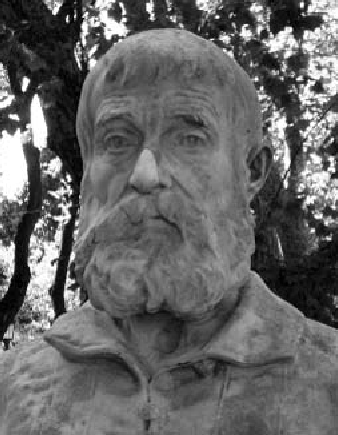
\includegraphics[width=\linewidth]{external/images/Tartaglia.png}
\end{image}%
\tcblower
\end{figureptx}%
Ferrari also knew how to compute the general solution of the \terminology{depressed quartic} so when he and his teacher \href{https://mathshistory.st-andrews.ac.uk/Biographies/Cardan}{Girolomo Cardano} (1501-1576) figured out how to depress a general quartic they had a complete solution of the general quartic as well.%
\begin{figureptx}{Figure}{Girolomo Cardano}{ThreeLessons_lesson-two-21}{}%
\index{Cardano, Girolomo!portrait of}%
\index{Portraits!Cardano}%
\begin{image}{0.325}{0.35}{0.325}{}%
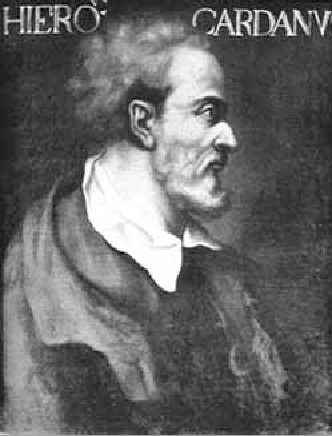
\includegraphics[width=\linewidth]{external/images/Cardan.png}
\end{image}%
\tcblower
\end{figureptx}%
Alas, their methods broke down entirely when they tried to solve the general quintic equation.  Unfortunately the rest of this story belongs in a course on Abstract Algebra, not Real Analysis.  But the lesson in this story applies to all of mathematics: Every problem solved is a new theorem which then becomes a tool for later use.  Depressing a cubic would have been utterly useless had not Tartaglia had a solution of the depressed cubic in hand.  The technique they used, with slight modifications, then allowed for a solution of the general quartic as well.%
\par
Keep this in mind as you proceed through this course and your mathematical education.  Every problem you solve is really a theorem, a potential tool that you can use later.  We have chosen the problems in this text deliberately with this in mind. Don't just solve the problems and move on.  Just because you have solved a problem does not mean you should stop thinking about it.  Keep thinking about the problems you've solved. Internalize them.  Make the ideas your own so that when you need them later you will have them at hand to use.%
\begin{problem}{Problem}{The Quadratic Formula.}{ThreeLessons_lesson-two-24}%
%
\begin{enumerate}[label={(\alph*)}]
\item{}Find \(M\) so that the substitution \(x=y-M\) depresses \hyperref[eq_GenCubic]{equation~({\xreffont\ref{eq_GenCubic}})}, the general cubic equation.  Then find \(p\) and \(q\) in terms of \(a\), \(b\), \(c\), and \(d\).%
\item{}Find \(K\) so that the substitution \(x=y-K\) depresses the general quartic equation.  Make sure you demonstrate how you obtained that value or why it works (if you guessed it).%
\item{}Find \(N\) so that the substitution \(x=y-N\) depresses a polynomial of degree \(n\).   Make sure you demonstrate how you obtained that value or why it works (if you guessed it).%
\end{enumerate}
%
\end{problem}
\begin{problem}{Problem}{Another Derivation of the Quadratic Formula.}{ThreeLessons_lesson-two-25}%
Here is yet another way to solve a quadratic equation.  Read the development below with pencil and paper handy.  Confirm all of the computations that are not completely transparent to you.  Then use your notes to present the solution with \emph{all} steps filled in.%
\begin{aside}{Aside}{}{ThreeLessons_lesson-two-25-3-2}%
Be sure you are clear on the purpose of this problem before you begin.  This is not about solving the Quadratic Equation.  You already know how to do that.  Our purpose here is to give you practice filling in the skipped details of mathematical exposition.  We've chosen this particular problem because it should be a comfortable setting for you, but this particular solution is probably outside of your previous experience.%
\end{aside}
Suppose that \(r_1\) and \(r_2\) are solutions of \(ax^2+bx+c=0\). Without loss of generality suppose that \(a>0\).  Suppose further that \(r_1\ge r_2\).  Then%
\begin{align*}
ax^2+bx+c \amp = a(x-r_1)(x-r_2)\\
\amp =
a\left[x^2-(r_1+r_2)x+(r_1+r_2)^2-(r_1-r_2)^2-3r_1r_2\right].
\end{align*}
%
\par
Therefore%
\begin{align}
r_1+r_2\amp = -\frac{b}{a}\label{eq_LagrangeQuadratic1}\\
\intertext{and}
r_1-r_2 \amp = \sqrt{\left(\frac{b}{a}\right)^2-\frac{4c}{a}}\text{.}\label{eq_LagrangeQuadratic2}
\end{align}
%
\par
Equations \hyperref[eq_LagrangeQuadratic1]{({\xreffont\ref{eq_LagrangeQuadratic1}})} and \hyperref[eq_LagrangeQuadratic2]{({\xreffont\ref{eq_LagrangeQuadratic2}})} can be solved simultaneously to yield%
\begin{align*}
r_1\amp =\frac{-b+\sqrt{b^2-4ac}}{2a}\\
r_2\amp =\frac{-b-\sqrt{b^2-4ac}}{2a}\text{.}
\end{align*}
%
\end{problem}
\end{sectionptx}
%
%
\typeout{************************************************}
\typeout{Section 1.3 Lesson Three}
\typeout{************************************************}
%
\begin{sectionptx}{Section}{Lesson Three}{}{Lesson Three}{}{}{ThreeLessons_lesson-three}
In the hustle and bustle of a typical college semester, with a lot of demands on your time and very little time to think, it becomes very easy to see each problem you solve as a small, isolated victory and then move on to the next challenge.  This is understandable.  Each problem you solve \emph{is} a small victory and you've every right to be proud of it.  But it is not isolated and it is a mistake to think that it is.%
\par
In his book \emph{How to Solve It} the mathematician and teacher \href{https://mathshistory.st-andrews.ac.uk/Biographies/Polya/}{George Polya} (1887\textendash{}1985) gave four steps for problem solving.  The steps may be paraphrased as%
\begin{enumerate}
\item{}Understand the problem.%
\item{}Formulate a plan.%
\item{}Execute the plan.%
\item{}Reflect on what you've done.%
\end{enumerate}
%
\begin{figureptx}{Figure}{George Polya}{ThreeLessons_lesson-three-4}{}%
\index{Portraits!Polya}%
\index{Polya, George!portrait of}%
\begin{image}{0.325}{0.35}{0.325}{}%
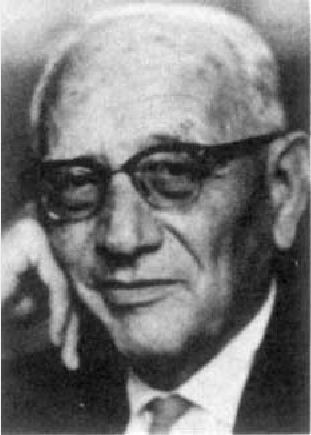
\includegraphics[width=\linewidth]{external/images/Polya.png}
\end{image}%
\tcblower
\end{figureptx}%
This process is iterative.  That is, once a plan is formulated and executed we often find that our plan was not up to the task. So we have to ask what went wrong, form a new plan and try again.  This is the fourth step: Reflect on what you've done.%
\par
Almost everyone remembers this fourth step when their plan \emph{doesn't} work.  After all, you've got to try again so you have to ask what went wrong.  But it is all too easy to neglect that crucial fourth step when the plan succeeds.  In that case, flush with success we usually move on to the next problem and start over from scratch.%
\par
This is a mistake.  Having solved a problem is no reason to stop thinking about it.%
\par
That fourth step is at least as important when we have succeeded as when we have failed.  Each time you solve a problem stop and ask yourself a few questions:%
\begin{itemize}[label=\textbullet]
\item{}Are there any easy consequences that follow from the result?%
\item{}How does it fit into the broader scheme of other problems you have solved?%
\item{}How might it be used in the future?%
\end{itemize}
%
\par
Also, notice the structure of the problem.  Some assumptions had to be made.  What were they?  Were they all necessary?  That is, did your solution use everything that was assumed?  If not, you may have something considerably more general than it at first appears to be.  What is that more general statement?  Even if you used all of the assumptions, was that really necessary?  Can you solve a similar problem with weaker assumptions?%
\par
Take a moment to pack all of these questions (and their answers) away in your mind so that when you see something similar in the future you will be reminded of it.  \emph{Don't} solve any problem and then forget it and move on.  The nature of mathematics is cumulative.  Remember, you are not here to accumulate grade points.  You are here to learn and understand the concepts and methods of mathematics, to gain ``mathematical maturity.'' Part of that maturation process is the accumulation of a body of facts (theorems), and techniques that can be used to prove new theorems (solve new problems).%
\par
This text has been written with the maturation process in mind. You will frequently find that the problems you solve today can be used to good effect in the ones you attempt tomorrow, but only if you remember them.  So take a moment after you've solved each problem to think about how it fits into the patterns you already know.  This is important enough to bear repeating: \emph{A problem, once solved, becomes a tool for solving subsequent problems!}%
\par
The purpose of the following sequence of problems is to help you become accustomed to this notion (if you aren't already).  It is a progression of results about prime numbers.  As you probably recall, a prime number is any integer greater than \(1\) whose only factors are itself and \(1\).  For example, \(2\), \(3\), \(5\), \(7\), \(11\) are prime, while \(4\), \(6\), \(9\) are not.  A major result about prime numbers is the following:%
\begin{theorem}{Theorem}{The Fundamental Theorem of Arithmetic.}{}{thm_FTA}%
Any integer greater than \(1\) is either prime or it is a product of prime numbers.  Furthermore, this prime decomposition is unique up to the order of the factors.%
\end{theorem}
We will not prove \hyperref[thm_FTA]{The Fundamental Theorem of Arithmetic}. We will assume that is is true and use it as a starting point to examine the following problems, eventually arriving at the result known as \hyperref[thm_FermatsLittleTheorem]{Fermat's Little Theorem}:%
\begin{theorem}{Theorem}{Fermat's Little Theorem.}{}{thm_FermatsLittleTheorem}%
\index{Fermat's Little Theorem}%
If \(p\) is a prime number then \(p\,|(n^p-n)\) for all positive integers \(n\).%
\end{theorem}
As you work through these problems, notice how each subsequent problem makes use of the previous results. The notation \(p\,|a\) simply means that the integer \(p\) divides the integer \(a\) with no remainder.%
\begin{problem}{Problem}{}{PROBLEMFermLittl1}%
Let \(p\) be a prime number and \(a, b\) positive integers such that \(p\, | (a\cdot b)\).  Show that \(p\,|a\) or \(p\,|b\).%
\par\smallskip%
\noindent\textbf{\blocktitlefont Hint}.\hypertarget{PROBLEMFermLittl1-3}{}\quad{}If \(p\,|a\) then we are done.  If not then notice that \(p\) is a prime factor of \(a\cdot b\).  What does the Fundamental Theorem of Arithmetic say about the prime factors of \(a\cdot b\) compared to the prime factors of \(a\) and \(b?\)%
\end{problem}
\begin{problem}{Problem}{}{PROBLEMFermLittl2}%
Let \(p\) be a prime number and let \(a_1, a_2, \ldots,
a_n\) be positive integers such that \(p\,|\left(a_1\cdot
a_2\cdot a_3\cdot\ldots\cdot a_n\right)\).%
\par
Use \hyperref[PROBLEMFermLittl1]{Problem~{\xreffont\ref{PROBLEMFermLittl1}}} to show that \(p\,|a_k\) for some \(k\in\{1, 2, 3, \ldots, n\}\).%
\par\smallskip%
\noindent\textbf{\blocktitlefont Hint}.\hypertarget{PROBLEMFermLittl2-3}{}\quad{}Use induction on \(n\) and the result of the previous problem.%
\end{problem}
\begin{problem}{Problem}{}{PROBLEMFermLittl3}%
Let \(p\) be a prime number and let \(k\) be an integer with \(1\le k\le p-1\).%
\par
Use \hyperref[PROBLEMFermLittl2]{Problem~{\xreffont\ref{PROBLEMFermLittl2}}} to prove that \(p\left|{p \choose{}k}\right.\), where \({p
\choose{}k}\) is the binomial coefficient \(\frac{p!}{k!(p-k)!}\).%
\par\smallskip%
\noindent\textbf{\blocktitlefont Hint}.\hypertarget{PROBLEMFermLittl3-3}{}\quad{}We know \(p\,|p\,!\), so \(p\,|{p \choose{}k}k!(p-k)!\). How does the previous result apply?%
\end{problem}
We now have all the machinery in place to prove one of the really cool theorems from number theory.%
\begin{problem}{Problem}{}{DRILLPROBLEMFermLittl4}%
Use \hyperref[PROBLEMFermLittl3]{Problem~{\xreffont\ref{PROBLEMFermLittl3}}} to show that \(p|(n^p-n)\) for all positive integers \(n\), thus proving \hyperref[thm_FermatsLittleTheorem]{Fermat's Little Theorem}.%
\par\smallskip%
\noindent\textbf{\blocktitlefont Hint}.\hypertarget{DRILLPROBLEMFermLittl4-3}{}\quad{}Use induction on \(n\).  To get from \(n\) to \(n+1\), use the binomial theorem on \((n+1)^p\) and the result of \hyperref[PROBLEMFermLittl3]{Problem~{\xreffont\ref{PROBLEMFermLittl3}}} .%
\end{problem}
\hyperref[thm_FermatsLittleTheorem]{Fermat's Little Theorem} is the foundational basis for a number of results in number theory and encryption.%
\begin{problem}{Problem}{}{ThreeLessons_lesson-three-23}%
Recall what we said above: Having solved a problem is no reason to stop thinking about it. Reflect upon your proof of \hyperref[thm_FermatsLittleTheorem]{Fermat's Little Theorem} by answering these questions.%
\begin{enumerate}[font=\bfseries,label=(\alph*),ref=\alph*]%
\item{}Will the result of Fermat's Little Theorem hold if \(p\) is not a prime number?%
\item{}If not, then which of the steps in the proof breaks down?%
\end{enumerate}%
\end{problem}
\end{sectionptx}
\end{chapterptx}
%
%
\typeout{************************************************}
\typeout{Chapter 2 Numbers, Real \(\left(\RR\right)\) and Rational \(\left(\QQ\right)\)}
\typeout{************************************************}
%
\begin{chapterptx}{Chapter}{Numbers, Real \(\left(\RR\right)\) and Rational \(\left(\QQ\right)\)}{}{Numbers, Real \(\left(\RR\right)\) and Rational \(\left(\QQ\right)\)}{}{}{NumbersRealRational}
\renewcommand*{\chaptername}{Chapter}
The set of real numbers (denoted, \(\RR\)) is badly named. The real numbers are no more or less real \textemdash{} in the non-mathematical sense that they exist \textemdash{} than any other set of numbers, just like the set of rational numbers (\(\QQ\)), the set of integers (\(\ZZ\)), or the set of natural numbers (\(\NN\)). The name ``real numbers'' is (almost) an historical anomaly not unlike the name ``Pythagorean Theorem'' which was actually known and understood long before Pythagoras lived.%
\par
When Calculus was being invented in the \(17\)th century, numbers were thoroughly understood, or so it was believed.%
\begin{aside}{Aside}{How Old is Calculus?}{NumbersRealRational-4}%
Some would say ``re-invented.'' See \hyperlink{russo96__forgot_revol}{[{\xreffont 13}]}, or \hyperlink{netz07__archim_codex}{[{\xreffont 9}]}.  %
\end{aside}
They were, after all, just numbers. Combine them. We call that addition. If you add them repeatedly we call it multiplication. Subtraction and division were similarly understood.%
\par
It was (and still is) useful to visualize these things in a more concrete way.  If we take a stick of length 2 and another of length 3 and lay them end-to-end we get a length of 5.  This is addition.  If we lay them end\textendash{}to\textendash{}end but at right angles then our two sticks are the length and width of a rectangle whose area is 6.  This is multiplication.%
\par
Of course measuring lengths with whole numbers has limitations, but these are not hard to fix. If we have a length (stick) of length 1 and another of length 2, then we can find another whose length when compared to 1 is the same (has the same proportion) as \(1\) is to \(2\). That number of course, is \(1/2\).%
\begin{figureptx}{Figure}{}{Fractions}{}%
\begin{image}{0.125}{0.75}{0.125}{}%
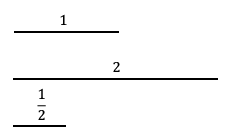
\includegraphics[width=\linewidth]{external/images/Fractions.png}
\end{image}%
\tcblower
\end{figureptx}%
Notice how fraction notation reflects the operation of comparing 1 to 2.  This comparison is usually referred to as the \terminology{ratio} of \(1\) to \(2\) so numbers of this sort are called \terminology{rational numbers.} The set of rational numbers is denoted \(\QQ\) for quotients.  In grade school they were introduced to you as fractions.  Once fractions are understood, this visualization using line segments (sticks) leads quite naturally to their representation with the rational number line.%
\begin{figureptx}{Figure}{The Rational Number Line}{RationalNumberLine}{}%
\begin{image}{0}{1}{0}{}%
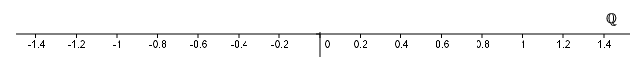
\includegraphics[width=\linewidth]{external/images/RationalNumberLine.png}
\end{image}%
\tcblower
\end{figureptx}%
This seems to work as a visualization because the \terminology{rational numbers} and the points on a line seem to share certain properties.  Chief among these is that between any two points on the rational line there is another point, just as between any two rational numbers there is another rational number.%
\begin{problem}{Problem}{}{NumbersRealRational-12}%
Let \(a, b, c, d\in\NN\) and find a rational number between \(a/b\) and \(c/d\).%
\end{problem}
This is all very clean and satisfying until we examine it just a bit closer.  Then it becomes quite mysterious.  Consider again the rational numbers \(a/b\) and \(c/d\).  If we think of these as lengths we can ask, "Is there a third length, say \(\alpha\), such that we can divide \(a/b\) into \(M\) pieces, each of length \(\alpha\) \emph{and also} divide \(c/d\) into \(N\) pieces each of length \(\alpha?\)" A few minutes thought should convince you that this is the same as the problem of finding a common denominator so \(\alpha=\frac{1}{bd}\) will work nicely.  (Confirm this yourself.)%
\par
You may be wondering what we're making all of this fuss about. \emph{Obviously} this is \emph{always} true.  In fact the previous paragraph gives an outline of a very nice little proof of this.  Here are the theorem and its proof presented formally.%
\begin{theorem}{Theorem}{}{}{thm_CommonDenominatorsExist}%
\index{common denominators}%
Suppose \(a\), \(b\), \(c\), and \(d\) are integers, with \(b, d \neq 0\). There is a number \(\alpha\in\QQ\) such that \(M\alpha=a/b\) and \(N\alpha=c/d\) where \(M\) and \(N\) are also integers.%
\end{theorem}
\begin{proof}{Proof}{}{NumbersRealRational-16}
To prove this theorem we will display \(\alpha\), \(M\) and \(N\).  It is your responsibility to confirm that these actually work.  Here they are: \(\alpha=1/bd\), \(M=ad\), and \(N=cb\).%
\end{proof}
\begin{problem}{Problem}{}{NumbersRealRational-17}%
Confirm that \(\alpha, M, \text{ and } N\) as given in the proof of \hyperref[thm_CommonDenominatorsExist]{Theorem~{\xreffont\ref{thm_CommonDenominatorsExist}}} satisfy the requirements of the theorem.%
\end{problem}
\hyperref[thm_CommonDenominatorsExist]{Theorem~{\xreffont\ref{thm_CommonDenominatorsExist}}} suggests the following very deep and important question: Are there lengths which can \emph{not} be expressed as the ratio of two integer lengths? The answer, of course, is yes. Otherwise we wouldn't have asked the question.  %
\par
One of the best known examples of such a number is the circumference of a circle with diameter 1. This is the number usually denoted by \(\pi\). But circles are extremely complex objects \textemdash{} they only seem simple because they are so familiar. Arising as it does from a circle, you would expect the number \(\pi\) to be very complex as well and this is true. In fact \(\pi\) is an exceptionally weird number for a variety of reasons. Let's start with something a little easier to think about.%
\par
\index{\(\sqrt{2}\)!is irrational} Squares are simple. Two sets of parallel lines at right angles, all of the same length. What could be simpler? If we construct a square with sides having length 1 then its diagonal has length \(\sqrt{2}\).%
\begin{figureptx}{Figure}{A construction of \(\sqrt{2}\)}{Sqrt2}{}%
\begin{image}{0.325}{0.35}{0.325}{}%
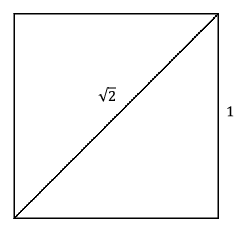
\includegraphics[width=\linewidth]{external/images/Sqrt2.png}
\end{image}%
\tcblower
\end{figureptx}%
This is a number which cannot be expressed as the ratio of two integers.  That is, it is \terminology{irrational}. This has been known since ancient times, but it is still quite disconcerting when first encountered.  It seems so counter\textendash{}intuitive that the intellect rebels.  ``This can't be right,'' it says. ``That's just crazy!''%
\par
Nevertheless it is true and we can prove it is true as follows.%
\par
What happens if we suppose that the square root of two \emph{can} be expressed as a ratio of integers? We will show that this leads irrevocably to a conclusion that is manifestly not true.%
\par
Suppose \(\sqrt{2}=a/b\) where \(a\) and \(b\) are integers. Suppose further that the fraction \(a/b\) is in lowest terms. \emph{This assumption is crucial because if \(a/b\) is in lowest terms we know that at most only one of them is even.}%
\par
So%
\begin{align*}
\frac{a}{b} \amp = \sqrt{2}.\\
\intertext{Squaring both sides gives:}
a^2 \amp = 2b^2.\\
\intertext{Therefore \(a^2\) is even. But if \(a^2\) is even then \(a\) must be even also (why?). If \(a\) is even then \(a=2k\) for some integer \(k\). Therefore}
4k^2\amp =2b^2\textit{ or}\\
2k^2\amp = b^2\text{.}
\end{align*}
%
\par
Therefore \(b^2\) is also even and so \(b\) must be even too. But this is impossible. We've just concluded that \(a\) and \(b\) are both even and this conclusion follows directly from our initial assumption that at most one of them could be even.%
\par
This is nonsense. Where is our error? It is not in any single step of our reasoning. That was all solid. Check it again to be sure.%
\par
Therefore our error must be in the initial assumption that \(\sqrt{2}\) could be expressed as a fraction. That assumption must therefore be false. In other words, \(\sqrt{2}\) cannot be so expressed.%
\begin{problem}{Problem}{Irrational Numbers.}{NumbersRealRational-30}%
Show that each of the following numbers is irrational:%
\begin{enumerate}[font=\bfseries,label=(\alph*),ref=\alph*]%
\item{}\(\sqrt{3}\)%
\item{}\(\sqrt{5}\)%
\item{}\(\sqrt[3]{2}\)%
\item{}\(i\) \((=\sqrt{-1})\)%
\item{}The square root of every positive integer which is not the square of an integer.%
\end{enumerate}%
\end{problem}
\begin{problem}{Problem}{}{NumbersRealRational-31}%
Determine if each of the following is always rational or always irrational. Justify your answers.%
\begin{enumerate}[font=\bfseries,label=(\alph*),ref=\alph*]%
\item{}The sum of two rational numbers.%
\item{}The sum of two irrational numbers.%
\item{}The sum of a rational and an irrational number.%
\end{enumerate}%
\end{problem}
\begin{problem}{Problem}{}{NumbersRealRational-32}%
\begin{enumerate}[font=\bfseries,label=(\alph*),ref=\alph*]%
\item{}Decide if it is  possible to have two rational numbers, \(a\) and \(b\), such that \(a^b\) is irrational. If so, display an example of such \(a\) and \(b\). If not, prove that it is not possible.%
\item{}Decide if it is possible to have two irrational numbers, \(a\) and \(b\), such that \(a^b\) is rational. If so, display an example of such \(a\) and \(b\). If not, prove that it is not possible.%
\par\smallskip%
\noindent\textbf{\blocktitlefont Hint}.\hypertarget{NumbersRealRational-32-5-2}{}\quad{}The number \(\left( \sqrt{2}\right)^{\sqrt{2}}\) must be either rational or irrational (why?). What can you conclude in each case?%
\end{enumerate}%
\end{problem}
\index{\(\sqrt{2}\)!meaning of} The fact that \(\sqrt{2}\) is not rational is cute and interesting but unless, like the Pythagoreans of ancient Greece, you have a strongly held religious conviction that all numbers are rational, it does not seem terribly important.  On the other hand, the very existence of \(\sqrt{2}\) raises some interesting questions.  For example what can the symbol \(4^{\sqrt{2}}\) possibly mean?  If the exponent were a rational number, say \(m/n\) with \(m, n \in \ZZ\), then clearly \(4^{m/n}=\sqrt[n]{4^m}\).  But since \(\sqrt{2}\neq m/n\) for \emph{any} integers \(m\) and \(n\) how do we interpret \(4^{\sqrt{2}}?\) Does it have any meaning at all? The more you think about this, the more puzzling the existence of irrational numbers becomes.  Suppose for example we reconsider the construction of a line segment of length \(\sqrt{2}\).  It is clear that the construction works and that we really can build such a line segment.  It exists.%
\par
Repeat the construction but this time let's put the base side on the rational line.%
\begin{figureptx}{Figure}{}{Sqrt2OnRatLine}{}%
\begin{image}{0.25}{0.5}{0.25}{}%
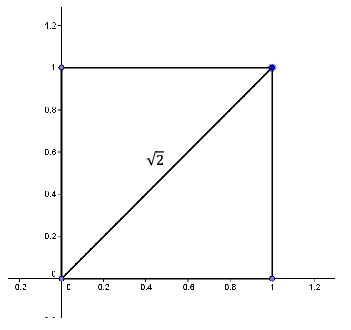
\includegraphics[width=\linewidth]{external/images/Sqrt2OnRatLine.png}
\end{image}%
\tcblower
\end{figureptx}%
We know that the diagonal of this square is \(\sqrt{2}\) as indicated.  And we know that \(\sqrt{2}\) is not a rational number.%
\par
Now leave the diagonal pinned at \((0,0)\) but allow it to rotate down so that it coincides with the \(x-\)axis.%
\begin{figureptx}{Figure}{}{Sqrt2Irrational}{}%
\begin{image}{0.25}{0.5}{0.25}{}%
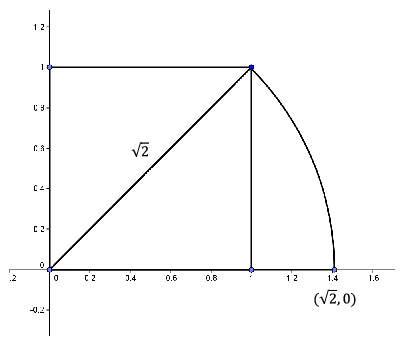
\includegraphics[width=\linewidth]{external/images/Sqrt2Irrational.png}
\end{image}%
\tcblower
\end{figureptx}%
The end of our diagonal will trace out an arc of the circle with radius \(\sqrt{2}\). When the diagonal coincides with the \(x-\)axis, its endpoint will obviously be the point \((\sqrt{2}, 0)\) as shown.%
\par
But wait! We're using the \emph{rational} number line for our \(x-\)axis. That means the only points on the \(x-\)axis are those that correspond to rational numbers (fractions). But we know that \(\sqrt{2}\) is not rational! Conclusion: There is no point \((\sqrt{2},0)\). It simply doesn't exist.%
\par
Put differently, there is a hole in the rational number line right where \(\sqrt{2}\) should be.%
\begin{figureptx}{Figure}{}{RationalLineWithHoles}{}%
\begin{image}{0}{1}{0}{}%
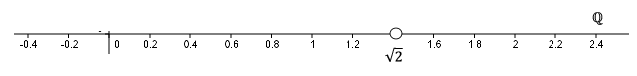
\includegraphics[width=\linewidth]{external/images/RationalLineWithHoles.png}
\end{image}%
\tcblower
\end{figureptx}%
This is weird,  but it's even worse than that!%
\par
Recall that between any two rational numbers there is always another.  This fact is what led us to represent the rational numbers with a line in the first place.%
\par
It's straightforward to show that \(\sqrt{3}\), \(\sqrt{5}\), etc. are all irrational too. So are \(\pi\) and \(e\), though they aren't as easy to show. It seems that the rational line has a bunch of holes in it. Infinitely many.%
\par
And yet, the following theorem is true%
\begin{theorem}{Theorem}{}{}{thm_IrrationalBetweenIrrationals}%
\index{\(\RR\)!real numbers exist between real numbers}%
%
\begin{enumerate}[label={(\alph*)}]
\item{}Between any two distinct real numbers there is a rational number.%
\item{}Between any two distinct real numbers there is an irrational number.%
\end{enumerate}
%
\end{theorem}
Both parts of this theorem rely on a judicious use of what is now called the \terminology{Archimedean Property} of the Real Number System, which can be formally stated as follows.%
\begin{principle}{Principle}{The Archimedean Property.}{}{ArchimedeanProperty}%
\index{Archimedean Property} Given any two positive real numbers, \(a\) and \(b\), there is a positive integer, \(n\) such that \(na>b\).%
\end{principle}
Physically this says that we can empty an ocean \(b\) with a teaspoon \(a\), provided we are willing to use the teaspoon a large number of times \(n\).%
\par
This is such an intuitively straightforward concept that it is easy to accept it without proof.  Until the invention of Calculus, and even for some time after that, it was simply assumed.  However as the foundational problems posed by the concepts of Calculus were understood and solved we were eventually led to a deeper understanding of the complexities of the real number system and the \terminology{Archimedean Property} is no longer taken as an unproved axiom. Rather, it is now understood to be a consequence of other axioms.  We will prove this in \hyperref[IVTandEVT-SupremumAndEVT]{Section~{\xreffont\ref{IVTandEVT-SupremumAndEVT}}}, but for now we will accept it as obviously true just as Archimedes did.%
\par
\index{Leibniz, Gottfried Wilhelm!and infinitesimals} With the invention of Calculus, mathematicians of the seventeenth century began to use objects which didn't satisfy the \terminology{Archimedean Property} (in fact, so did Archimedes). As we shall see in the next chapter, when Leibniz wrote the first paper on his version of the Calculus, he followed this practice by explicitly laying out rules for manipulating infinitely small quantities (infinitesimals).  These were taken to be actual numbers which are not zero and yet smaller than any real number. The notation he used was \(\dx{ x}\) (an infinitely small displacement in the \(x\) direction), and \(\dx{ y}\) (an infinitely small displacement in the \(y\) direction).  These symbols should look familiar to you.  They are the same \(\dx{
y}\) and \(\dx{ x}\) used to form the derivative symbol \(\dfdx{y}{x}\) that you learned about in Calculus.%
\par
Mathematicians of the seventeenth and eighteenth centuries made amazing scientific and mathematical progress exploiting these infinitesimals, even though they were foundationally suspect. No matter how many times you add the infinitesimal \(\dx{ x}\) to itself the result will not be bigger than, say \(10^{-1000}\), which is very bizarre.%
\par
\index{Lagrange, Joseph-Louis} When foundational issues came to the forefront, infinitesimals fell somewhat out of favor. You probably didn't use them very much in Calculus. Most of the time you probably used the prime notation, \(f^\prime(x)\) introduced by Lagrange in the eighteenth century. Some of the themes in this book are: Why differentials fell out of favor, what were they replaced with and how the modern notations you learned in Calculus evolved over time.%
\par
The idea of infinitesimals was revisited in the twentieth century by the logician \href{https://mathshistory.st-andrews.ac.uk/Biographies/Robinson/}{Abraham Robinson} (1918\textendash{}1974). In his book \pubtitle{Non\textendash{}Standard Analysis} \hyperlink{robinson74__non_stand_analy}{[{\xreffont 12}]} Robinson was able to put the idea of infinitesimals on a solid logical foundation, but in the \(18\)th century the notion of infinitesimal numbers was shaky to say the very least. Nonetheless mathematicians of the time were able to profitably exploit the idea of infinitely small quantities. We will come back to this saga in later chapters, but for now we return to \hyperref[thm_IrrationalBetweenIrrationals]{Theorem~{\xreffont\ref{thm_IrrationalBetweenIrrationals}}}.%
\begin{figureptx}{Figure}{Abraham Robinson}{FIGURERobinsonPortrait}{}%
\begin{image}{0.325}{0.35}{0.325}{}%
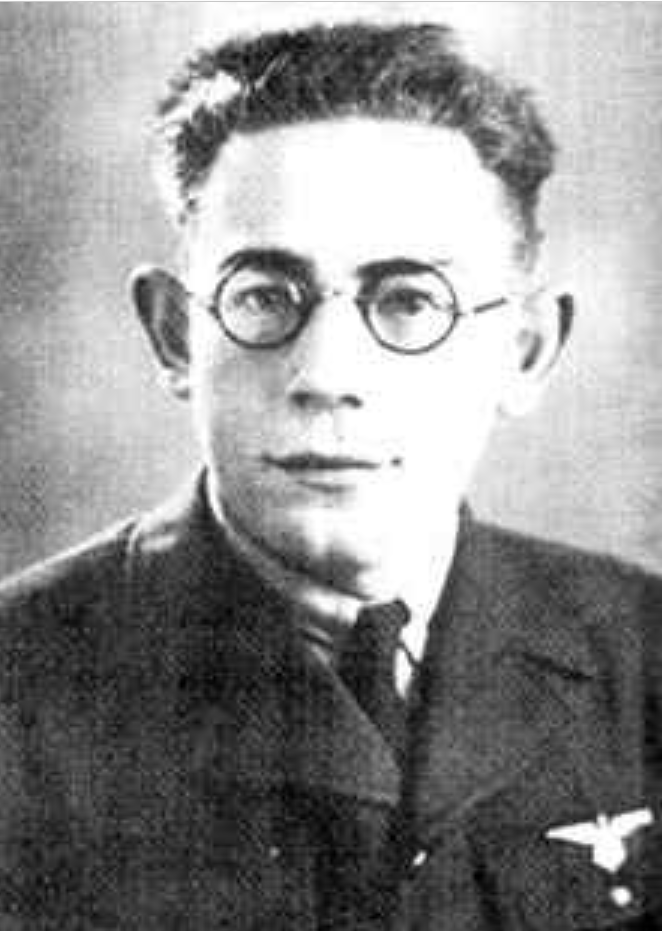
\includegraphics[width=\linewidth]{external/images/Robinson.png}
\end{image}%
\tcblower
\end{figureptx}%
\begin{proof}{Proof}{Sketch of Proof.}{NumbersRealRational-57}
We will outline the proof of part (a) of \hyperref[thm_IrrationalBetweenIrrationals]{Theorem~{\xreffont\ref{thm_IrrationalBetweenIrrationals}}} and indicate how it can be used to prove part (b).%
\par
Let \(\alpha\) and \(\beta\) be real numbers with \(\alpha > \beta\). There are two cases.%
\begin{itemize}[label=\textbullet]
\item{}\lititle{Case 1:.}\par%
\(\alpha-\beta > 1\). In this case there is at least one integer between \(\alpha\) and \(\beta\). Since integers are rational we are done.%
\item{}\lititle{Case 2:.}\par%
\(\alpha-\beta \le 1\).  In this case, by the \terminology{Archimedean Property} there is a positive integer, say \(n\), such that \(n(\alpha-\beta) = n\alpha-n\beta
> 1\).  Now there will be an integer between \(n\alpha\) and \(n\beta\).  You should now be able to find a rational number between \(\alpha\) and \(\beta\).%
\end{itemize}
%
\end{proof}
For part (b), divide \(\alpha\) and \(\beta\) by any positive irrational number and apply part a.  There are a couple of details to keep in mind.  These are considered in the following problem.%
\begin{problem}{Problem}{}{NumbersRealRational-59}%
\begin{enumerate}[font=\bfseries,label=(\alph*),ref=\alph*]%
\item{}Prove that the product of a nonzero rational number and an irrational number is irrational.%
\item{}Use the result of part (a) to prove \hyperref[thm_IrrationalBetweenIrrationals]{Theorem~{\xreffont\ref{thm_IrrationalBetweenIrrationals}}}.%
\end{enumerate}%
\end{problem}
As a practical matter, the existence of irrational numbers isn't really very important.  In light of \hyperref[thm_IrrationalBetweenIrrationals]{Theorem~{\xreffont\ref{thm_IrrationalBetweenIrrationals}}}, any irrational number can be approximated arbitrarily closely by a rational number.  So if we're designing a bridge and \(\sqrt{2}\) is needed we just use \(1.414\) instead.  The error introduced is less than \(0.001 =1/1000\) so it probably doesn't matter.%
\par
But from a theoretical point of view this is devastating.  When Calculus was invented, the rational numbers were suddenly not up to the task of justifying the concepts and operations we needed to work with.%
\par
\index{Newton, Isaac!foundation of Calculus} Newton explicitly founded his version of Calculus on the assumption that we can think of variable quantities as being generated by a continuous motion.  If our number system has holes in it such continuous motion is impossible because we have no way to jump over the gaps.  So Newton simply postulated that there were no holes.  He filled in the hole where \(\sqrt{2}\) should be.  He simply said, yes there is a number there called \(\sqrt{2}\) and he did the same with all of the other holes.%
\par
To be sure there is no record of Newton explicitly saying, ``Here's how I'm going to fill in the holes in the rational number line.'' Along with everyone else at the time, he simply assumed there were no holes and moved on.  It took about \(200\) years of puzzling and arguing over the contradictions, anomalies and paradoxes to work out the consequences of that apparently simple assumption.  The task may not yet be fully accomplished, but by the 20th century the properties of the real number system (\(\RR\)) as an extension of the rational number system (\(\QQ\)) were well understood.  Here are both systems visualized as lines:%
\begin{figureptx}{Figure}{\(\RR\) and \(\QQ\)}{RandQ}{}%
\begin{image}{0}{1}{0}{}%
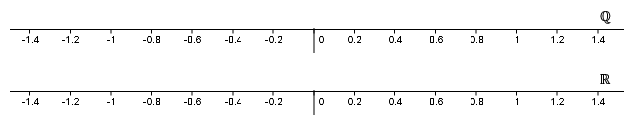
\includegraphics[width=\linewidth]{external/images/RandQ.png}
\end{image}%
\tcblower
\end{figureptx}%
Impressive, no?%
\par
The reason they look alike, except for the labels \(\RR\) and \(\QQ\) of course, is that our ability to draw sketches of the objects we're studying utterly fails when we try to sketch \(\RR\), as different from \(\QQ\).  All of the holes in \(\QQ\) really are there, but the non-holes are packed together so closely that we can't separate them in a drawing. This inability to sketch the objects we study will be a frequent source of frustration.%
\par
Of course, this will not stop us from drawing sketches.  When we do, our imaginations will save us because it is possible to imagine \(\QQ\) as distinct from \(\RR\).  But put away the idea that a sketch is an accurate representation of anything.  At best our sketches will only be aids to the imagination.%
\par
So, at this point we will simply assume the existence of the real numbers.  We will assume also that they have all of the properties that we are used to.  This is perfectly acceptable as long as we make our assumptions explicit.  However we need to be aware that, so far, the existence and properties of the real numbers is an assumption that has not been logically derived.  Any time we make an assumption we need to be prepared to either abandon it completely if we find that it leads to nonsensical results, or to re-examine the assumption in the light of these results to see if we can find another assumption that subsumes the first and explains the (apparently) nonsensical results.%
\end{chapterptx}
%
%
\typeout{************************************************}
\typeout{Chapter 3 Calculus in the 17th and 18th Centuries}
\typeout{************************************************}
%
\begin{chapterptx}{Chapter}{Calculus in the 17th and 18th Centuries}{}{Calculus in the 17th and 18th Centuries}{}{}{CalcIn17th18thCentury}
\renewcommand*{\chaptername}{Chapter}
%
%
\typeout{************************************************}
\typeout{Section 3.1 Newton and Leibniz Get Started}
\typeout{************************************************}
%
\begin{sectionptx}{Section}{Newton and Leibniz Get Started}{}{Newton and Leibniz Get Started}{}{}{CalcIn17th18thCentury-NewtLeibStart}
%
%
\typeout{************************************************}
\typeout{Subsection  Leibniz' Calculus Rules}
\typeout{************************************************}
%
\begin{subsectionptx}{Subsection}{Leibniz' Calculus Rules}{}{Leibniz' Calculus Rules}{}{}{sec_leibn-calc-rules}
\index{Leibniz, Gottfried Wilhelm!first Calculus publication} The rules for Calculus were first laid out in the 1684 paper \textit{Nova methodus pro maximis et minimis, itemque tangentibus, quae nec fractas nec irrationales, quantitates moratur, et singulare pro illi calculi genus} (A New Method for Maxima and Minima as Well as Tangents, Which is Impeded Neither by Fractional Nor by Irrational Quantities, and a Remarkable Type of Calculus for This) written by \href{https://mathshistory.st-andrews.ac.uk/Biographies/Leibniz/}{Gottfried Wilhelm Leibniz} (1646\textendash{}1716).  Leibniz started with subtraction.  That is, if \(x_1\) and \(x_2\) are very close together then their difference, \(\Delta
x=x_2-x_1\), is very small.  He expanded this idea to say that if \(x_1\) and \(x_2\) are \emph{infinitely} close together (but still distinct) then their difference \(\dx{ x}\), is infinitesimally small (but not zero).%
\begin{figureptx}{Figure}{Gottfried Wilhelm Leibniz}{sec_leibn-calc-rules-3}{}%
\index{Leibniz, Gottfried Wilhelm!portrait of}%
\index{Portraits!Leibniz}%
\begin{image}{0.325}{0.35}{0.325}{}%
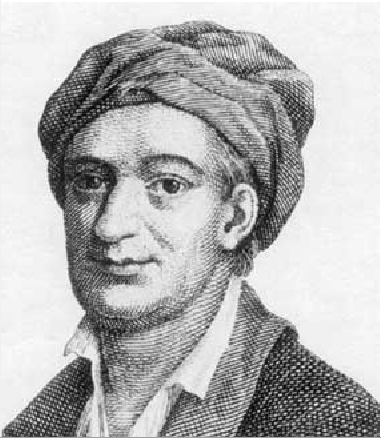
\includegraphics[width=\linewidth]{external/images/Leibniz.png}
\end{image}%
\tcblower
\end{figureptx}%
\begin{aside}{Aside}{\textit{Calculus Differentialis}.}{sec_leibn-calc-rules-4}%
This translates, loosely, as the ``Calculus of Differences''.%
\end{aside}
This idea is logically very suspect and Leibniz knew it.  But he also knew that when he used his \textit{calculus differentialis} he was getting correct answers to some very hard problems.  So he persevered.%
\par
Leibniz called both \(\Delta x\) and \(\dx{ x}\) differentials (Latin for difference) because he thought of them as, essentially, the same thing.  Over time it has become customary to refer to the infinitesimal \(\dx{ x}\) as a differential, and to reserve the word difference and the notation \(\Delta x\) for the finite case.  This is why Calculus is often called \emph{Differential Calculus}.%
\par
In his paper Leibniz gave rules for dealing with these infinitely small differentials.  Specifically, given a variable quantity \(x\), \(\dx{x}\) represented an infinitesimal change in \(x\).  Differentials are related via the slope of the tangent line to a curve.  That is, if \(y=f(x)\), then \(\dx{ y}\) and \(\dx{ x}\) are related by%
\begin{equation*}
\dx{ y}=\text{ (slope of the tangent line) } \cdot \dx{ x}\text{.}
\end{equation*}
%
\par
Leibniz then divided by \(\dx{ x}\) giving%
\begin{equation*}
\dfdx{y}{x}= \text{ (slope of the tangent line). }
\end{equation*}
%
\par
\index{Newton, Isaac} The elegant and expressive notation Leibniz invented was so useful that it has been retained through the years despite some profound changes in the underlying concepts.  For example, Leibniz and his contemporaries would have viewed the symbol \(\dfdx{y}{x}\) as an actual quotient of infinitesimals, whereas today we define it via the limit concept first suggested by Newton.%
\par
\index{Leibniz, Gottfried Wilhelm!differentiation rules} As a result Leibniz' rules governing his differentials are very modern in appearance:%
\begin{align*}
\dx{(\text{ constant } )}\amp =0\\
\dx{(z-y+w+x)}\amp =\dx{ z}-\dx{ y}+\dx{ w}+\dx{ x}\\
\dx{(xv)}\amp =x\dx{ v}+v\dx{ x}\\
\dx{\left(\frac{v}{y}\right)}\amp =\frac{y\dx{ v}-v\dx{ y}}{yy}\\
\intertext{and, when \(a\) is an integer:}
\dx{(x^a)}\amp =ax^{a-1}\dx{ x}\text{.}
\end{align*}
%
\par
Leibniz states these rules without proof: ``. . . the demonstration of all this will be easy to one who is experienced in such matters . . .''. Mathematicians in Leibniz's day would have been expected to understand intuitively that if \(c\) is a constant, then%
\begin{equation*}
\dx(c)=c-c=0\text{.}
\end{equation*}
Likewise, \(\dx(x+y)=\dx{x}+\dx{y}\) is really an extension of%
\begin{equation*}
\underbrace{(x_2+y_2)-(x_1+y_1)}_{\Delta
(x+y)}=\underbrace{(x_2-x_1)}_{\Delta
x}+\underbrace{(y_2-y_1)}_{\Delta{y}} \text{.}
\end{equation*}
%
\end{subsectionptx}
%
%
\typeout{************************************************}
\typeout{Subsection  Leibniz's Approach to the Product Rule}
\typeout{************************************************}
%
\begin{subsectionptx}{Subsection}{Leibniz's Approach to the Product Rule}{}{Leibniz's Approach to the Product Rule}{}{}{LeibnizProductRule}
\index{Leibniz, Gottfried Wilhelm} The explanation of the product rule using differentials is a bit more involved, but Leibniz expected that mathematicans would be fluent enough to derive it.  The product \(p=xv\) can be thought of as the area of the following rectangle%
\begin{figureptx}{Figure}{}{fig1}{}%
\begin{image}{0.25}{0.5}{0.25}{}%
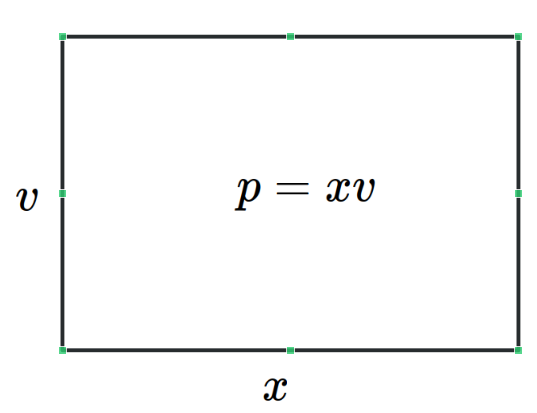
\includegraphics[width=\linewidth]{external/images/fig1-1.png}
\end{image}%
\tcblower
\end{figureptx}%
With this in mind, \(\dx{ p}=\dx{(xv)}\) can be thought of as the change in area when \(x\) is changed by \(\dx{ x}\) and \(v\) is changed by \(\dx{ v}\).  This can be seen as the L shaped region in the following drawing.%
\begin{figureptx}{Figure}{}{fig2}{}%
\begin{image}{0.05}{0.9}{0.05}{}%
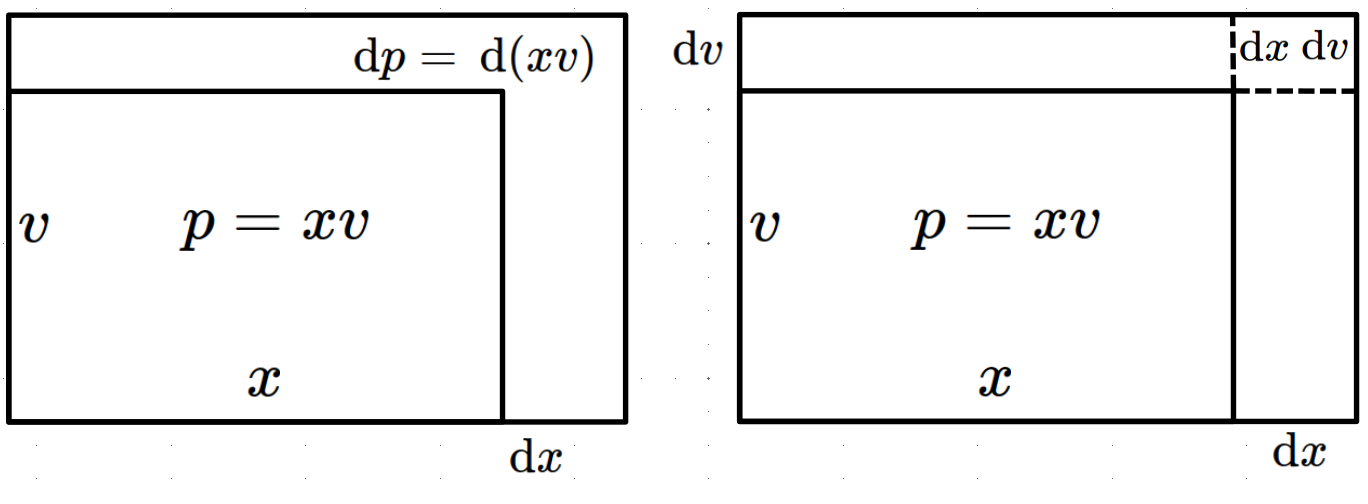
\includegraphics[width=\linewidth]{external/images/fig2-1.png}
\end{image}%
\tcblower
\end{figureptx}%
By dividing the L shaped region into 3 rectangles we obtain%
\begin{equation}
\dx{(xv)}=x\dx{ v}+v\dx{ x}+\dx{ x}\,\dx{ v}\text{.}\label{eq_LeibnizProductRule}
\end{equation}
%
\par
Even though \(\dx{ x}\) and \(\dx{ v}\) are infinitely small, Leibniz reasoned that \(\dx{ x}\,\dx{ v}\) is \emph{even more} infinitely small (quadratically infinitely small?)  compared to \(x\dx{ v}\) and \(v\dx{ x}\) and can thus be ignored leaving%
\begin{equation*}
\dx{ (xv)}=x\dx{ v}+v\dx{ x}\text{.}
\end{equation*}
%
\par
\index{Newton, Isaac} You should feel some discomfort at the idea of simply tossing the product \(\dx{ x}\,\dx{ v}\) aside because it is ``comparatively small.'' This means you have been well trained, and have thoroughly internalized Newton's dictum \hyperlink{newton45__sir_isaac_two_treat_quadr}{[{\xreffont 10}]}: ``The smallest errors may not, in mathematical matters, be scorned.'' It is logically untenable to toss aside an expression just because it is small.  Even less so should we be willing to ignore an expression on the grounds that it is ``infinitely smaller'' than another quantity which is itself ``infinitely small.''%
\par
Newton and Leibniz both knew this as well as we do.  But they also knew that their methods worked.  They gave verifiably correct answers to problems which had, heretofore, been completely intractable.  It is the mark of their genius that both men persevered in spite of the very evident difficulties their methods entailed.%
\end{subsectionptx}
%
%
\typeout{************************************************}
\typeout{Subsection  Newton's Approach to the Product Rule}
\typeout{************************************************}
%
\begin{subsectionptx}{Subsection}{Newton's Approach to the Product Rule}{}{Newton's Approach to the Product Rule}{}{}{NewtonsApproach}
\href{https://mathshistory.st-andrews.ac.uk/Biographies/Newton/}{Isaac Newton's} (1643\textendash{}1727) approach to Calculus \textemdash{} his `Method of Fluxions' \textemdash{} depended fundamentally on motion.  He conceived of variables (fluents) as changing (flowing or fluxing) in time.  The rate of change of a fluent he called a fluxion.  As a theoretical foundation both Leibniz's and Newton's approaches have fallen out of favor, although both are still universally used as a conceptual approach, a ``way of thinking,'' about the ideas of Calculus.%
\begin{figureptx}{Figure}{Isaac Newton}{Newton}{}%
\index{Newton, Isaac!portrait of}%
\index{Portraits!Newton}%
\begin{image}{0.325}{0.35}{0.325}{}%
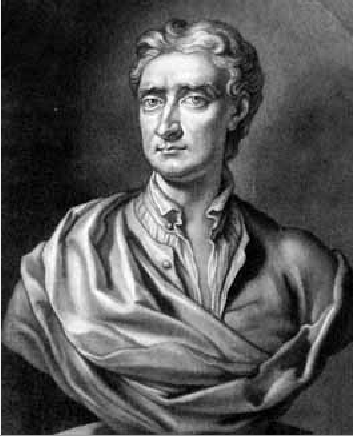
\includegraphics[width=\linewidth]{external/images/Newton.png}
\end{image}%
\tcblower
\end{figureptx}%
In \pubtitle{Philosophiae naturalis principia mathematica} (this is usually shortened to \pubtitle{Principia}) Newton ``proved'' the Product Rule as follows: Let \(x\) and \(v\) be ``flowing quantites'' and consider the rectangle, \(R\), whose sides are \(x\) and \(v\).  \(R\) is also a flowing quantity and we wish to find its fluxion (derivative) at any time.%
\par
First we increment \(x\) and \(v\) by the half\textendash{}increments \(\frac{\Delta
x}{2}\) and \(\frac{\Delta v}{2}\) respectively.  Then the corresponding half\textendash{}increment of \(R\) is%
\begin{equation}
\frac{\Delta R}{2}=\left(x+\frac{\Delta x}{2}\right)\left(v+\frac{\Delta v}{2}\right) = xv + x\frac{\Delta v}{2} + v\frac{\Delta x}{2} +\frac{\Delta x\Delta v}{4}\text{.}\label{eq_prodruleinc}
\end{equation}
%
\par
Now decrement \(x\) and \(v\) by the same amounts:%
\begin{equation}
-\frac{\Delta R}{2}=\left(x-\frac{\Delta x}{2}\right)\left(v-\frac{\Delta v}{2}\right) = xv - x\frac{\Delta v}{2} - v\frac{\Delta x}{2} + \frac{\Delta x\Delta v}{4}\text{.}\label{eq_prodruledec}
\end{equation}
%
\par
Subtracting  \hyperref[eq_prodruledec]{equation~({\xreffont\ref{eq_prodruledec}})} from  \hyperref[eq_prodruleinc]{equation~({\xreffont\ref{eq_prodruleinc}})} gives%
\begin{equation*}
\Delta R = x\Delta v + v\Delta x
\end{equation*}
which is the total change of \(R = xv\) over the intervals \(\Delta x\) and \(\Delta v\) and also recognizably the Product Rule.%
\par
This argument is no better than Leibniz's as it relies heavily on the number \(1/2\) to make it work.  If we take any other increments in \(x\) and \(v\) whose total lengths are \(\Delta x\) and \(\Delta v\) it will simply not work.  Try it and see.%
\par
In Newton's defense, he wasn't really trying to justify his mathematical methods in the \pubtitle{Principia}.  His attention was on physics, not math, so he was really just trying to give a convincing demonstration of his methods.  You may decide for yourself how convincing his demonstration is.%
\par
\index{Lagrange, Joseph-Louis} Notice that there is no mention of limits of difference quotients or derivatives.  In fact, the term derivative was not coined until 1797, by Lagrange as we will see in \hyperref[PowerSeriesQuestions-TaylorsFormula]{Section~{\xreffont\ref{PowerSeriesQuestions-TaylorsFormula}}} .  In a sense, these topics were not necessary at the time, as Leibniz and Newton both assumed that the curves they dealt with had tangent lines and, in fact, Leibniz explicitly used the tangent line to relate two differential quantities.  This was consistent with the thinking of the time and for the duration of this chapter we will also assume that all quantities are differentiable.  As we will see later this assumption leads to difficulties.%
\par
Both Newton and Leibniz were satisfied that their Calculus provided answers that agreed with what was known at the time.  For example the formulas%
\begin{equation*}
\dx{ \left(x^2\right)}=\dx{\left(xx\right)}=x\dx{ x}+x\dx{
x}=2x\dx{ x} 
\end{equation*}
and%
\begin{equation*}
\dx{\left(x^3\right)}=\dx{\left(x^2x\right)}=x^2\dx{
x}+x\dx{\left(x^2\right)}=x^2+x\left(2x\dx{
x}\right)=3x^2\dx{ x}\text{,}
\end{equation*}
were results that had been derived by others using other methods.%
\begin{problem}{Problem}{}{NewtonsApproach-12}%
Assume \(n\) is a positive integer.%
\begin{enumerate}[font=\bfseries,label=(\alph*),ref=\alph*]%
\item{}Use Leibniz' product rule \(\dx{\left(xv\right)}=x\dx{v}+v\dx{x}\) to show that%
\begin{equation*}
\dx{\left(x^n\right)}=nx^{n-1}\dx{x}
\end{equation*}
%
\item{}Suppose \(y=x^{-1}=\frac{1}{x}\), Use Leibniz' product rule to show%
\begin{equation*}
dy=-1x^{-2}\dx{x}
\end{equation*}
%
\item{}Use the product rule and the result of part (b) to derive the quotient rule%
\begin{equation*}
d\left(\frac{v}{x}\right)=\frac{x\dx{v}-v\dx{x}}{x^2}
\end{equation*}
%
\item{}Use the quotient rule to show that%
\begin{equation*}
d\left(x^{-n}\right)=-nx^{-n-1}\dx{x}
\end{equation*}
%
\end{enumerate}%
\end{problem}
\begin{problem}{Problem}{}{NewtonsApproach-13}%
Suppose \(y=x^{\frac{p}{q}}\) with \(q\neq 0\), where \(p\) and \(q\) are integers. Show that%
\begin{equation*}
\dx{y}=\dx{
\left(x^{\frac{p}{q}}\right)}=\frac{p}{q}x^{\frac{p}{q}-1}\dx{
x}\text{.}
\end{equation*}
%
\end{problem}
To prove the worth of his Calculus Leibniz also provided applications.  As an example he derived Snell's Law of Refraction from his Calculus rules as follows.%
\begin{figureptx}{Figure}{\href{https://mathshistory.st-andrews.ac.uk/Biographies/Snell/}{Willebrord Snell} (1580\textendash{}1626)}{FIGURESnellPortrait}{}%
\begin{image}{0.325}{0.35}{0.325}{}%
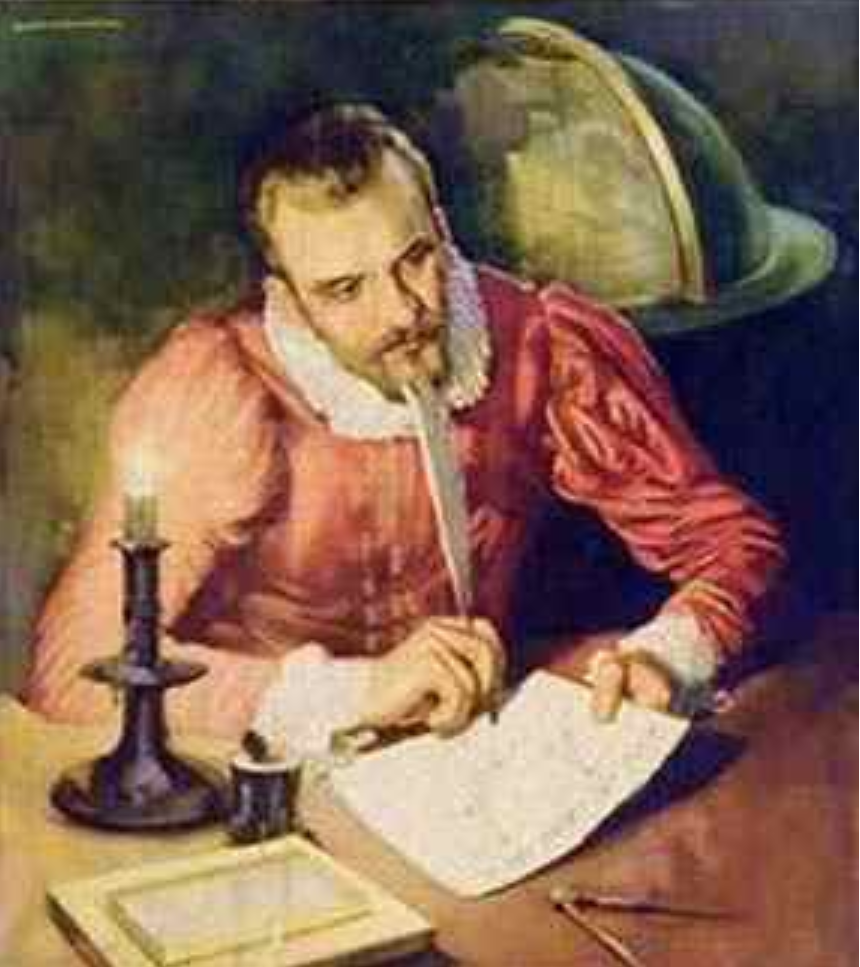
\includegraphics[width=\linewidth]{external/images/Snell.png}
\end{image}%
\tcblower
\end{figureptx}%
Given that light travels through air at a speed of \(v_a\) and travels through water at a speed of \(v_w\) the problem is to find the fastest path from point \(A\) to point \(B\).%
\begin{figureptx}{Figure}{}{snellfig}{}%
\begin{image}{0.225}{0.55}{0.225}{}%
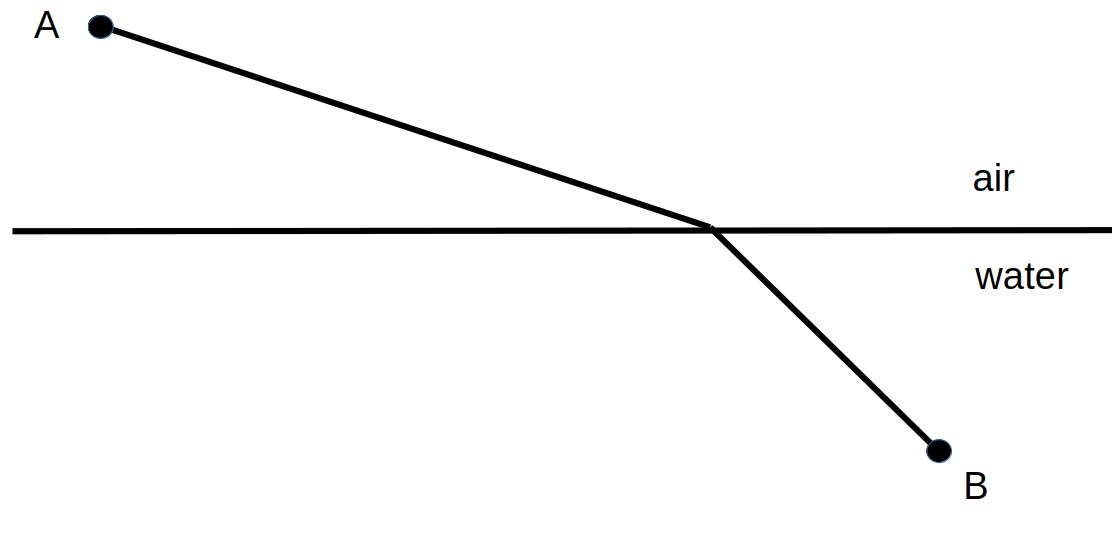
\includegraphics[width=\linewidth]{external/images/snellfig-1.png}
\end{image}%
\tcblower
\end{figureptx}%
According to \href{https://en.wikipedia.org/wiki/Fermat\%27s_principle}{Fermat's Principle of Least Time}, this fastest path is the one that light will travel.%
\par
Using the fact that \(\text{ Time }=\frac{\text{Distance}}{\text{Velocity}}\) and the labeling in the picture below we can obtain a formula for the time \(T\) it takes for light to travel from \(A\) to \(B\).%
\begin{figureptx}{Figure}{}{snellfig2}{}%
\begin{image}{0.225}{0.55}{0.225}{}%
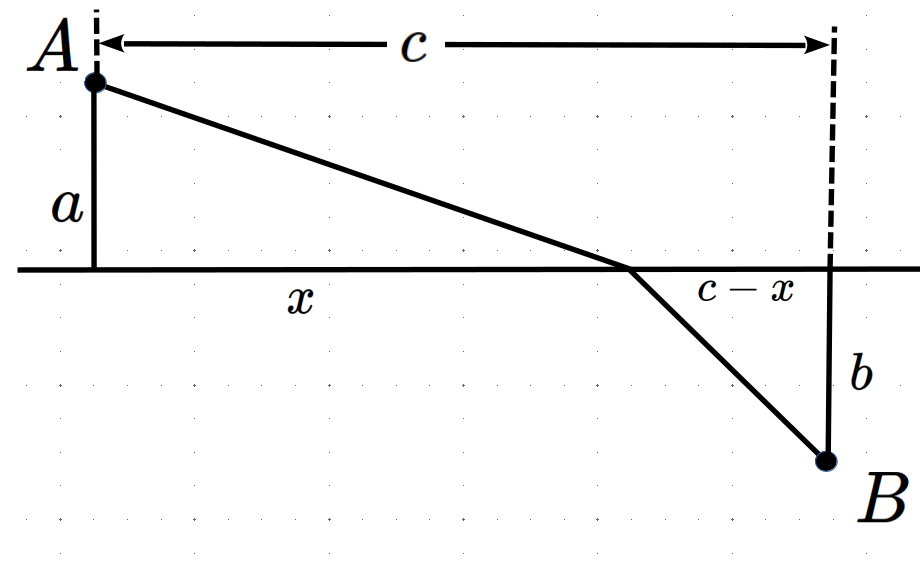
\includegraphics[width=\linewidth]{external/images/snellfig2-1.png}
\end{image}%
\tcblower
\end{figureptx}%
%
\begin{equation*}
T=\frac{\sqrt{x^2+a^2}}{v_a}+\frac{\sqrt{(c-x)^2+b^2}}{v_w}
\end{equation*}
%
\par
Using the rules of Leibniz's Calculus, we obtain%
\begin{align*}
\dx{ T}\amp = \left[\frac{1}{v_a}\frac{1}{2}\left(x^2+a^2\right)^{-\frac{1}{2}} (2x)+\frac{1}{v_w}\frac{1}{2}((c-x)^2+b^2)^{-\frac{1}{2}}(2(c-x)(-1))\right] \dx{x}\\
\amp =\left[\frac{1}{v_a}\frac{x}{\sqrt{x^2+a^2}}-\frac{1}{v_w}\frac{c-x}{\sqrt{(c-x)^2+b^2}}\right]\dx{ x}\text{.}
\end{align*}
%
\par
Using the fact that at the minimum value for \(T\), \(\dx{
T}=0\), we see that the fastest path from \(A\) to \(B\) must satisfy%
\begin{equation*}
\frac{1}{v_a}\frac{x}{\sqrt{x^2+a^2}}=\frac{1}{v_w}\frac{c-x}{\sqrt{(c-x)^2+b^2}}\text{.}
\end{equation*}
%
\begin{figureptx}{Figure}{}{snellfig3}{}%
\begin{image}{0.225}{0.55}{0.225}{}%
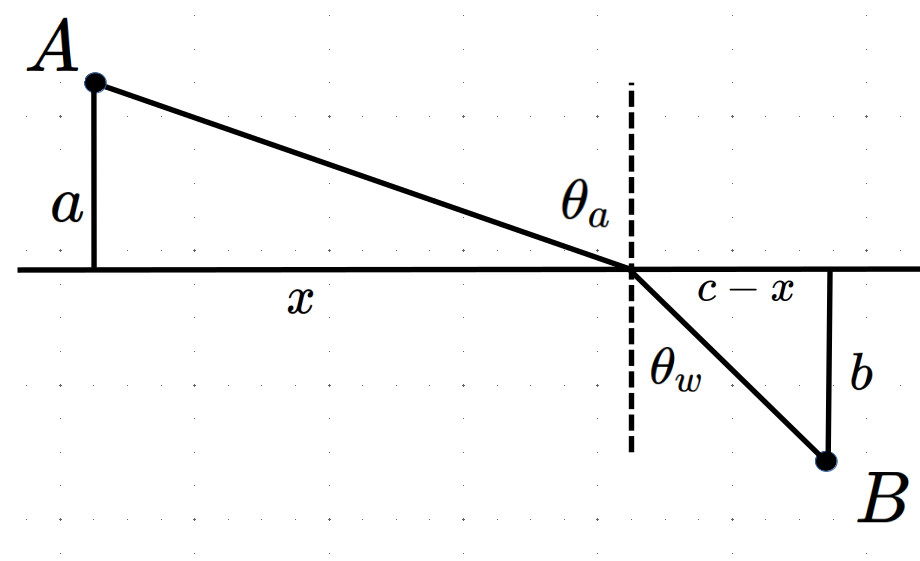
\includegraphics[width=\linewidth]{external/images/snellfig3-1.png}
\end{image}%
\tcblower
\end{figureptx}%
From \hyperref[snellfig3]{Figure~{\xreffont\ref{snellfig3}}} we see that the path that light travels must satisfy \(\frac{\sin\theta_a}{v_a}=\frac{\sin\theta_w}{v_w}\) which is Snell's Law.%
\par
\index{Bernoulli, Johann}\index{Brachistochrone problem, the} To compare 18th century and modern techniques we will consider \href{https://mathshistory.st-andrews.ac.uk/Biographies/Bernoulli_Johann/}{Johann Bernoulli's} (1667\textendash{}1748) solution of the \href{https://mathshistory.st-andrews.ac.uk/HistTopics/Brachistochrone/}{Brachistochrone Problem}.  In 1696, Bernoulli posed and solved, the Brachistochrone problem: To find the shape of a frictionless wire joining points \(A\) and \(B\) so that the time it takes for a bead to slide down under the force of gravity is as small as possible.%
\begin{figureptx}{Figure}{}{brachfig1}{}%
\begin{image}{0.225}{0.55}{0.225}{}%
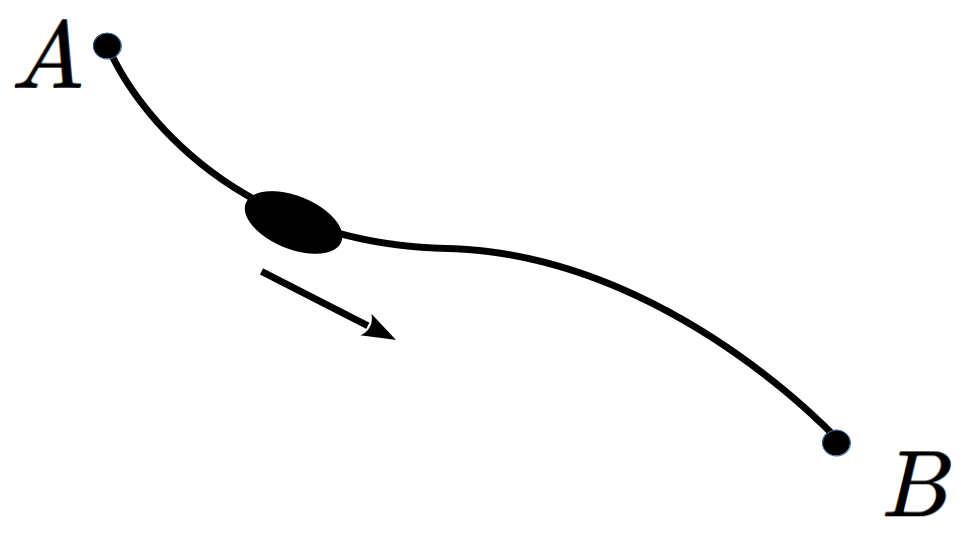
\includegraphics[width=\linewidth]{external/images/brachfig1-1.png}
\end{image}%
\tcblower
\end{figureptx}%
\index{Bernoulli, Johann!Bernoulli's challenge} Bernoulli posed this ``path of fastest descent'' problem to challenge the mathematicians of Europe and used his solution to demonstrate the power of Leibniz' Calculus as well as his own ingenuity.%
\begin{quote}%
I, Johann Bernoulli, address the most brilliant mathematicians in the world. Nothing is more attractive to intelligent people than an honest, challenging problem, whose possible solution will bestow fame and remain as a lasting monument. Following the example set by Pascal, Fermat, etc., I hope to gain the gratitude of the whole scientific community by placing before the finest mathematicians of our time a problem which will test their methods and the strength of their intellect. If someone communicates to me the solution of the proposed problem, I shall publicly declare him worthy of praise. \hyperlink{Bernoulli_bio_mactutor}{[{\xreffont 11}]}%
\end{quote}
\begin{figureptx}{Figure}{Johann Bernoulli}{NewtonsApproach-30}{}%
\index{Bernoulli, Johann!portrait of}%
\index{Portraits!Johann Bernoulli}%
\begin{image}{0.325}{0.35}{0.325}{}%
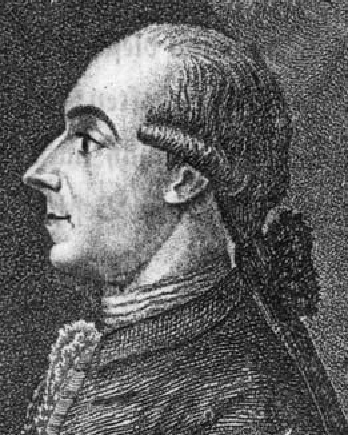
\includegraphics[width=\linewidth]{external/images/BernoulliJohann.png}
\end{image}%
\tcblower
\end{figureptx}%
\index{Bernoulli, Jacob}\index{Newton, Isaac} In addition to Johann's, solutions were obtained from Newton, Leibniz, Johann's brother Jacob Bernoulli, and the Marquis de l'Hopital \hyperlink{struik69__sourc_book_mathem}{[{\xreffont 15}]}.  At the time there was an ongoing and very vitriolic controversy raging over whether Newton or Leibniz had been the first to invent Calculus.  As an advocate for Leibniz, Bernoulli did not believe Newton would be able to solve the problem using his fluxions. So this challenge was in part an attempt to embarrass Newton.  However Newton solved it easily.%
\par
At this point in his life Newton had all but quit science and mathematics and was fully focused on his administrative duties as Master of the Mint.  Due in part to rampant counterfeiting, England's money had become severely devalued and the nation was on the verge of economic collapse.  The solution was to recall all of the existing coins, melt them down, and strike new ones.  As Master of the Mint this job fell to Newton \hyperlink{levenson09__newton_count}{[{\xreffont 8}]}.  As you might imagine this was a rather Herculean task.  Nevertheless, according to his niece (and housekeeper):%
\begin{quote}%
When the problem in 1696 was sent by Bernoulli\textendash{}Sir I.N. was in the midst of the hurry of the great recoinage and did not come home till four from the Tower very much tired, but did not sleep till he had solved it, which was by four in the morning.%
\end{quote}
He is reported to have complained, ``I do not love . . . to be . . . teezed by forreigners about Mathematical things'' \hyperlink{dunham90__journ_throug_genius}{[{\xreffont 2}]}.%
\par
Newton submitted his solution anonymously, presumably to avoid more controversy. Nevertheless the methods he used were so distinctively Newton's that Bernoulli is said to have exclaimed ``\textit{Tanquam ex ungue leonem}.''%
\begin{aside}{Aside}{Translation: \textit{Tanquam ex ungue leonem}.}{NewtonsApproach-36}%
``I know the lion by his claw.''%
\end{aside}
\index{Brachistochrone problem, the!Bernoulli's solution} Newton's solution was clever but it doesn't provide any insights we'll be interested in so we will focus on Bernoulli's ingenious solution which starts, interestingly enough, with Snell's Law of Refraction.  He begins by considering the stratified medium in the following figure, where an object travels with velocities \(v_1, v_2, v_3, \ldots\) in the various layers.%
\begin{figureptx}{Figure}{}{brachfig2}{}%
\begin{image}{0.225}{0.55}{0.225}{}%
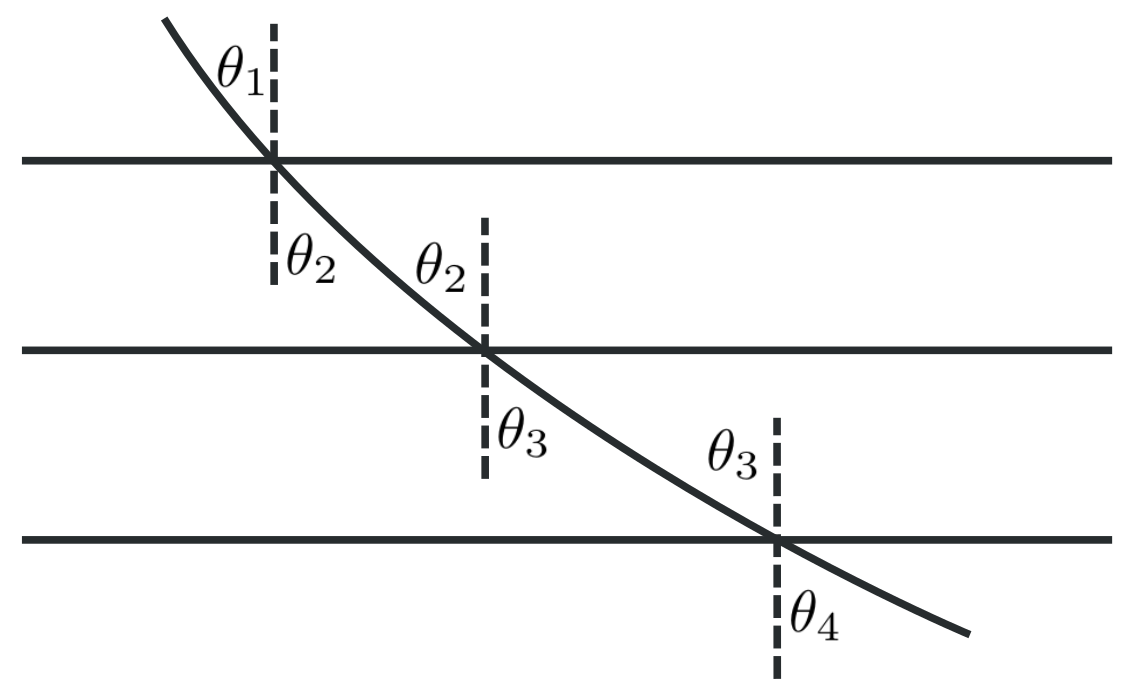
\includegraphics[width=\linewidth]{external/images/brachfig2-1.png}
\end{image}%
\tcblower
\end{figureptx}%
By repeatedly applying Snell's Law he concluded that the fastest path must satisfy%
\begin{equation*}
\frac{\sin \theta_1}{v_1}=\frac{\sin \theta_2}{v_2}=\frac{\sin\theta_3}{v_3}=\cdots\text{.}
\end{equation*}
%
\par
In other words, the ratio of the sine of the angle that the curve makes with the vertical and the speed remains constant along this fastest path.%
\par
If we think of a continuously changing medium as stratified into infinitesimal layers and extend Snell's law to an object whose speed is constantly changing, then along the fastest path, the ratio of the sine of the angle that the curve's tangent makes with the vertical, \(\alpha\), and the speed, \(v\), must remain constant,%
\begin{equation*}
\frac{\sin\alpha}{v}=c
\end{equation*}
as in \hyperref[snellfig4]{Figure~{\xreffont\ref{snellfig4}}} below.%
\begin{figureptx}{Figure}{}{snellfig4}{}%
\begin{image}{0.3}{0.4}{0.3}{}%
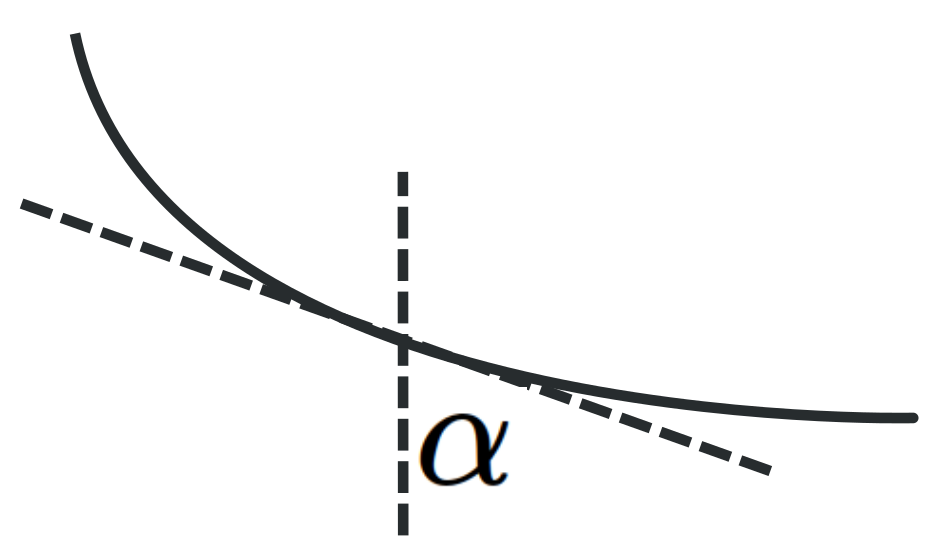
\includegraphics[width=\linewidth]{external/images/snellfig4-1.png}
\end{image}%
\tcblower
\end{figureptx}%
If we include the horizontal and vertical axes and let \(P\) denote the position of the bead at a particular time then we have the following picture.%
\begin{figureptx}{Figure}{}{snellfig5}{}%
\begin{image}{0.225}{0.55}{0.225}{}%
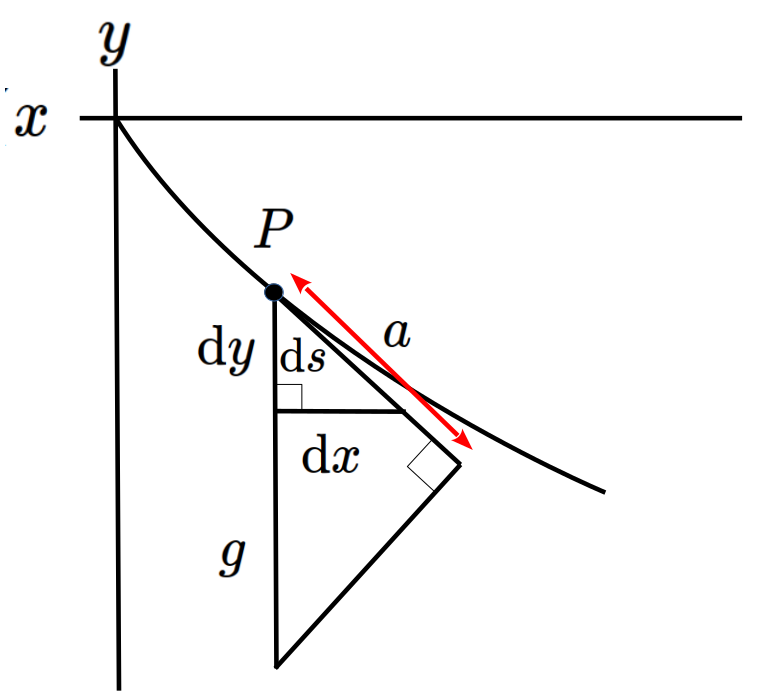
\includegraphics[width=\linewidth]{external/images/snellfig5-1.png}
\end{image}%
\tcblower
\end{figureptx}%
In \hyperref[snellfig5]{Figure~{\xreffont\ref{snellfig5}}}, \(s\) denotes the length that the bead has traveled down to point \(P\) (that is, the arc length of the curve from the origin to that point) and \(a\) denotes the tangential component of the acceleration due to gravity \(g\).  Since  acceleration is the rate of change of velocity with respect to time we see that%
\begin{equation*}
\dfdx{v}{t}=a\text{.}
\end{equation*}
%
\par
To get a sense of how physical problems were approached using Leibniz's Calculus we will use the above equation to show that \(v=\sqrt{2gy}\).%
\par
By similar triangles we have \(\frac{a}{g}=\frac{\dx{ y}}{\dx{ s}}\). As a student of Leibniz, Bernoulli would have regarded \(\frac{\dx{ y}}{\dx{ s}}\) as a fraction so%
\begin{equation*}
a\dx{s}  = g\dx{y}
\end{equation*}
and since acceleration is the rate of change of velocity we have%
\begin{equation}
\frac{\dx{ v}}{\dx{ t}}\dx{ s}  = g\dx{ y}\text{.}\label{EQUATIONDifferentialDemo}
\end{equation}
In the seventeenth, eighteenth, and even well into the nineteenth centuries, European mathematicians regarded \(\dx{ v}, \dx{ t}\), and \(\dx{ s}\) as infinitesimally small numbers which nevertheless obey all of the usual rules of algebra. Thus they would simply  rearrange \hyperref[EQUATIONDifferentialDemo]{equation~({\xreffont\ref{EQUATIONDifferentialDemo}})},  to get%
\begin{equation*}
\frac{\dx{s}}{\dx{t}}\dx{ v}  = g\dx{y}\text{.}
\end{equation*}
Since \(\frac{\dx{ s}}{\dx{ t}}\) is the rate of change of position with respect to time it is, in fact, the velocity of the bead. That is%
\begin{equation*}
v\dx{ v}  = g\dx{ y}\text{.}
\end{equation*}
Bernoulli would have interpreted this as a statement that two rectangles of height \(v\) and \(g\), with respective widths \(\dx{ v}\) and \(\dx{ y}\) have equal area. Summing (integrating) all such rectangles we g et:%
\begin{align*}
\int{}v\dx{ v} \amp = \int{}g\dx{ y}\\
\frac{v^2}{2} \amp = gy
\end{align*}
or%
\begin{equation}
v=\sqrt{2gy}\text{.}\label{eq_brach_vel}
\end{equation}
%
\par
You are undoubtedly uncomfortable with the cavalier manipulation of infinitesimal quantities you've just witnessed, so we'll pause for a moment now to compare a modern development of \hyperref[eq_brach_vel]{equation~({\xreffont\ref{eq_brach_vel}})} to Bernoulli's.  As before we begin with the equation:%
\begin{align*}
\frac{a}{g}\amp = \dfdx{y}{s}\\
a \amp = g\dfdx{y}{s}.\\
\intertext{Moreover, since acceleration is the derivative of velocity this is the same as:}
\dfdx{v}{t} \amp = g\dfdx{y}{s}.\\
\intertext{Now observe that by the Chain Rule \(\dfdx{v}{t} =
\dfdx{v}{s}\dfdx{s}{t}\). The physical interpretation of this formula is that velocity will depend on \(s\), how far down the wire the bead has moved, but that the distance traveled will depend on how much time has elapsed. Therefore}
\dfdx{v}{s}\dfdx{s}{t} \amp = g\dfdx{y}{s}\\
\intertext{or}
\dfdx{s}{t}\dfdx{v}{s} \amp = g\dfdx{y}{s}\\
\intertext{and since \(\dfdx{s}{t} = v\) we have}
v\dfdx{v}{s} \amp = g\dfdx{y}{s}\\
\intertext{Integrating both sides with respect to \(s\) gives:}
\int{}v\dfdx{v}{s}d s \amp = g\int{}\dfdx{y}{s}d s\\
\int{}vd v \amp = g\int{}d y\\
\intertext{and integrating gives}
\frac{v^2}{2} \amp = gy
\end{align*}
as before.%
\par
\index{Leibniz, Gottfried Wilhelm} In effect, in the modern formulation we have traded the simplicity and elegance of differentials for a comparatively cumbersome repeated use of the Chain Rule.  No doubt you noticed when taking Calculus that in the differential notation of Leibniz, the Chain Rule looks like we are simply ``canceling'' a factor in the top and bottom of a fraction: \(\dfdx{y}{u}\dfdx{u}{x} = \dfdx{y}{x}\).  This is because for 18th century mathematicians, that is exactly what it was, and Leibniz designed his notation to reflect that viewpoint.%
\par
To put it another way, 18th century mathematicians wouldn't have recognized a need for what we call the Chain Rule because this operation was a triviality for them.  Just reduce the fraction.  This begs the question: Why did we abandon such a clear and simple interpretation of our symbols in favor of the comparatively more cumbersome modern interpretation?  This is one of the questions we will try to answer in this course.%
\par
Returning to the Brachistochrone problem we observe that%
\begin{align}
\frac{\sin\alpha}{v} \amp = c\notag\\
\intertext{and since \(\sin\alpha = \frac{d x}{d s}\)   we see that}
\frac{\frac{d x}{d s}}{\sqrt{2gy}} \amp = c\notag\\
\frac{d x}{\sqrt{2gy(ds)^2}} \amp = c\notag\\
\frac{d x}{\sqrt{2gy\left[(d x)^2+(d y)^2\right]}} \amp = c\text{.}\label{eq_Brachistochrone}
\end{align}
%
\par
Bernoulli was then able to solve this differential equation.%
\begin{problem}{Problem}{}{NewtonsApproach-53}%
Show that the equations \(x=\frac{\phi-\sin
\phi}{4gc^2},\,y=\frac{1-\cos \phi}{4gc^2}\) satisfy equation \hyperref[eq_Brachistochrone]{equation~({\xreffont\ref{eq_Brachistochrone}})}. Bernoulli recognized this solution to be an inverted cycloid, the curve traced by a fixed point on a circle as the circle rolls along a horizontal surface.%
\end{problem}
This illustrates the state of Calculus in the late 1600s and early 1700s; the foundations of the subject were a bit shaky but there was no denying its power.%
\end{subsectionptx}
\end{sectionptx}
%
%
\typeout{************************************************}
\typeout{Section 3.2 Power Series as Infinite Polynomials}
\typeout{************************************************}
%
\begin{sectionptx}{Section}{Power Series as Infinite Polynomials}{}{Power Series as Infinite Polynomials}{}{}{ExponentAdditionProperty}
\index{polynomials!infinite} Applied to polynomials, the rules of differential and integral Calculus are straightforward.  Indeed, differentiating and integrating polynomials represent some of the easiest tasks in a Calculus course.  For example, computing \(\int(7-x+x^2)\dx{
x}\) is relatively easy compared to computing \(\int\sqrt[3]{1+x^3}\dx{ x}\).  Unfortunately, not all functions can be expressed as a polynomial.  For example, \(f(x)=\sin x\) cannot be since a polynomial has only finitely many roots and the sine function has infinitely many roots, namely \(\{n\pi|\,n\in\ZZ\}\).  A standard technique in the 18th century was to write such functions as an ``infinite polynomial,'' or what today we refer to as a \terminology{power series}.  Unfortunately an ``infinite polynomial'' is a much more subtle object than a mere polynomial, which by definition is finite.  For now we will not concern ourselves with these subtleties. Instead we will follow the example of our forebears and manipulate all ``polynomial\textendash{}like'' objects (finite or infinite) as if they are polynomials.%
\begin{definition}{Definition}{}{def_PowerSeries}%
\index{power series!definition}%
\index{Definition!power series}%
A \terminology{power series centered at \(\boldsymbol{a}\)} is a series of the form%
\begin{equation*}
\sum_{n=0}^\infty a_n(x-a)^n=a_0+a_1(x-a)+a_2(x-a)^2+\cdots\text{.}
\end{equation*}
%
\end{definition}
Thus a power series centered around zero has the form%
\begin{equation*}
\sum_{n=0}^\infty a_nx^n \text{.}
\end{equation*}
In this section we will focus on power series centered around zero. In \hyperref[SECTIONPowSerWOTaylor]{the next section} we will look at power series centered about points other than zero. \(0\).%
\begin{paragraphs}{A useful comment on notation:.}{ExponentAdditionProperty-5}%
The most advantageous way to represent a power series is using summation notation since there can be no doubt about the pattern in the terms.  After all, this notation contains a formula for the general term.  However, there are instances where summation notation is not practical.  In these cases, it is acceptable to indicate the sum by supplying the first few terms and using ellipses (the three dots).  If this is done, then enough terms must be included to make the pattern clear to the reader.%
\end{paragraphs}%
\par\medskip
\index{series!Geometric series!naive derivation} Returning to our definition of a power series, consider the power series%
\begin{equation*}
\sum_{n=0}^\infty x^n=1+x+x^2+\cdots \text{.}
\end{equation*}
If we multiply this power series by \((1-x)\), we obtain%
\begin{align*}
(1-x)(1+x+x^2+\cdots)=(1+\amp{}x+x^2+\cdots)\\
-(\amp{}x+x^2+x^3+\cdots)\\
=1.\ \ \ \ \amp{}
\end{align*}
%
\par
Dividing by \(1-x\) gives us the power series representation%
\begin{equation}
\frac{1}{1-x}=1+x+x^2+\cdots\text{,}\label{EQUATIONGeometricSeries}
\end{equation}
which is known as the \terminology{Geometric Series}.%
\par
For each value of \(x\) a \terminology{power series} reduces to a different ordinary (numerical) \terminology{series}. For example, if we substitute \(x=\frac{1}{10}\) into the left side of \hyperref[EQUATIONGeometricSeries]{equation~({\xreffont\ref{EQUATIONGeometricSeries}})}, we obtain the (numerical) \terminology{series}%
\begin{align*}
1+\frac{1}{10}+\left(\frac{1}{10}\right)^2+\left(\frac{1}{10}\right)^3+
\cdots\amp{}=1+0.1+0.01+0.001+0.0001+\cdots\\
\amp{}=1.1111\cdots.
\end{align*}
But substituting into the right side yields%
\begin{equation*}
\frac{1}{1-\frac{1}{10}}=\frac{10}{9}. 
\end{equation*}
%
\par
If these computations are valid then it must be that \(1.111\ldots=\frac{10}{9}\), which seems weird, but you can verify it by entering \(\frac{10}{9}\) into any calculator.%
\par
If \(1.111\ldots=\frac{10}{9}\), then subtracting \(1\) from both sides and multiplying by \(3\) gives%
\begin{equation*}
0.333\ldots = \frac{1}{3}
\end{equation*}
which has probably come up on your calculator more than once. But what seems wierder still is that if we multiply by \(3\) again we get%
\begin{equation*}
0.999\ldots
=1\text{,}
\end{equation*}
which seems like nonsense. It simply can't be true, can it? What do you think? Is \(0.999\ldots =1\) or that just nonsense?  Either way it is clear that the real numbers \(\left(\RR\right) \) hide deeper mysteries than the irrationality of \(\sqrt{2}\).%
\par
There are other issues with these formal manipulations too. Substituting \(x=1\) or \(x=2\) into \hyperref[EQUATIONGeometricSeries]{equation~({\xreffont\ref{EQUATIONGeometricSeries}})} yields the questionable results%
\begin{equation*}
\frac{1}{0}=1+1+1+\cdots \text{  and  } \frac{1}{-1}=1+2+2^2+\cdots\text{.}
\end{equation*}
%
\begin{aside}{Aside}{Formal Manipulation.}{ExponentAdditionProperty-12}%
When we say ``formal manipulations'' we mean that we will perform purely algebraic operations on an given expression without concerning ourselves (much) about whether the operations make sense in context. We will formalize them in \hyperref[TaylorSeries]{Chapter~{\xreffont\ref{TaylorSeries}}}%
\end{aside}
A power series representation of our function seems to work in some cases, but not in others. Obviously we are missing something important here, though it may not be clear exactly what. For now, we will continue to follow the example of our 18th century predecessors.  That is, for the rest of this section we will use formal manipulations to obtain and use power series representations of various functions.  Keep in mind that this is all highly suspect until we can resolve problems like those we've just seen.%
\par
Power series became an important tool in analysis in the 1700s. By representing various functions as power series they could be dealt with as if they were (infinite) polynomials.  The following is an example.%
\begin{example}{Example}{}{ExponentAdditionProperty-15}%
Solve the following Initial Value problem: Find \(y(x)\) given that%
\begin{align*}
\frac{\dx{ y}}{\dx{
x}}=y,\amp{}\amp{}y(0)=1.
\end{align*}
%
\begin{aside}{Aside}{}{ExponentAdditionProperty-15-2-2}%
A few seconds of thought should convince you that the solution of this problem is \(y(x) = e^x\).  We will ignore this for now in favor of emphasising the technique.%
\end{aside}
Assuming the solution can be expressed as a power series we have%
\begin{equation*}
y=\sum_{n=0}^\infty
a_nx^n=a_0+a_1x+a_2x^2+\cdots \text{.}
\end{equation*}
%
\par
Differentiating gives us%
\begin{equation*}
\frac{\dx{ y}}{\dx{
x}}=a_1+2a_2x+3a_3x^2+4a_4x^3+\ldots \text{.}
\end{equation*}
%
\par
Since \(\frac{\dx{ y}}{\dx{ x}}=y\) we see that%
\begin{equation*}
a_1=a_0\,,\,2a_2=a_1\,,\,3a_3=a_2\,,\,\ldots,\,na_n=a_{n-1}\,,\ldots\text{.}
\end{equation*}
%
\par
This leads to the relationship%
\begin{equation*}
a_n=\frac{1}{n}a_{n-1}=\frac{1}{n(n-1)}a_{n-2}=\cdots=\frac{1}{n!}a_0\text{.}
\end{equation*}
%
\par
Thus the power series solution of the differential equation is%
\begin{equation*}
y=\sum_{n=0}^\infty\frac{a_0}{n!}x^n
=a_0\sum_{n=0}^\infty\frac{1}{n!}x^n \text{.}
\end{equation*}
%
\par
Using the initial condition \(y(0)=1\), we get \(1=a_0(1+0+\frac{1}{2!}0^2+\cdots)=a_0\).  Thus the solution to the initial problem is \(y=\sum_{n=0}^\infty\frac{1}{n!}x^n\).  Let's call this function \(E(x)\).  Then by definition%
\begin{equation}
E(x)=\sum_{n=0}^\infty\frac{1}{n!}x^n=1+\frac{x^1}{1!}+\frac{x^2}{2!}+\frac{x^3}{3!}+\,\ldots\text{.}\label{EQUATIONExpSeries}
\end{equation}
%
\end{example}
Let's examine some properties of this function.  The first property is clear from the definition.%
\par
\terminology{Property 1}. \(E(0)=1\)%
\par
\terminology{Property 2}. \(E(x+y)=E(x)E(y)\).%
\par
To see this we multiply the two series together, so we have%
\begin{align}
E(x)E(y) =\amp \left(\sum_{n=0}^\infty\frac{1}{n!}x^n\right)\left(\sum_{n=0}^\infty\frac{1}{n!}y^n\right)\label{eq_ExponentAdditionProperty}\\
=\amp \left(\frac{x^0}{0!}+\frac{x^1}{1!}+\frac{x^2}{2!}+\frac{x^3}{3!}+\,\ldots\right)\left(\frac{y^0}{0!}+\frac{y^1}{1!}+\frac{y^2}{2!}+\frac{y^3}{3!}+\,\ldots\right)\notag\\
=\amp \frac{x^0}{0!}\frac{y^0}{0!}+\frac{x^0}{0!}\frac{y^1}{1!}+\frac{x^1}{1!}\frac{y^0}{0!}+\frac{x^0}{0!}\frac{y^2}{2!}+\frac{x^1}{1!}\frac{y^1}{1!}+\frac{x^2}{2!}\frac{y^0}{0!}\notag\\
\amp{}\ \ \         +\frac{x^0}{0!}\frac{y^3}{3!}+\frac{x^1}{1!}\frac{y^2}{2!}+\frac{x^2}{2!}\frac{y^1}{1!}+\frac{x^3}{3!}\frac{y^0}{0!}+\,\ldots\notag\\
=\amp\frac{x^0}{0!}\frac{y^0}{0!}+\left(\frac{x^0}{0!}\frac{y^1}{1!}+ \frac{x^1}{1!}\frac{y^0}{0!}\right)\notag\\
\amp{}\ \ \         +\left(\frac{x^0}{0!}\frac{y^2}{2!}+\frac{x^1}{1!}\frac{y^1}{1!}+\frac{x^2}{2!}\frac{y^0}{0!}\right)\notag\\
\amp{}\ \ \ \ \ \        +\left(\frac{x^0}{0!}\frac{y^3}{3!}+\frac{x^1}{1!}\frac{y^2}{2!}+\frac{x^2}{2!}\frac{y^1}{1!}+\frac{x^3}{3!}\frac{y^0}{0!}\right)+\,\ldots\notag\\
=\amp\frac{1}{0!}+\frac{1}{1!}\left(\frac{1!}{0!1!}x^0y^1+\frac{1!}{1!0!}x^1y^0\right)\notag\\
\amp{}\ \ \        +\frac{1}{2!}\left(\frac{2!}{0!2!}x^0y^2+\frac{2!}{1!1!}x^1y^1+\frac{2!}{2!0!}x^2y^0\right)\notag\\
\amp{}\ \ \ \ \ \        +\frac{1}{3!}\left(\frac{3!}{0!3!}x^0y^3+\frac{3!}{1!2!}x^1y^2+\frac{3!}{2!1!}x^2y^1+\frac{3!}{3!0!}x^3y^0\right)+\ldots\notag\\
=\amp \frac{1}{0!}+\frac{1}{1!}\left(\binom{1}{0}x^0y^1+\binom{1}{1}x^1y^0\right)\notag\\
\amp{}\ \ \        +\frac{1}{2!}\left(\binom{2}{0}x^0y^2+\binom{2}{1}x^1y^1+\binom{2}{2}x^2y^0\right)\notag\\
\amp{}\ \ \ \ \ \        +\frac{1}{3!}\left(\binom{3}{0}x^0y^3+\binom{3}{1}x^1y^2+\binom{3}{2}x^2y^1+\binom{3}{3}x^3y^0\right)+\ldots\notag\\
=\amp \frac{1}{0!}+\frac{1}{1!}\left(x+y\right)^1+\frac{1}{2!}\left(x+y\right)^2+\frac{1}{3!}\left(x+y\right)^3+\ldots\notag
\end{align}
so that, finally%
\begin{equation}
E(x)E(y) =  E(x+y)\text{.}\label{ExponentAdditionProperty-19-2}
\end{equation}
%
\par
\terminology{Property 3}. If \(m\) is a positive integer then \(E(mx)=\left(E(x\right))^m\). In particular, \(E(m)=\left(E(1)\right)^m\).%
\begin{problem}{Problem}{}{ExponentAdditionProperty-21}%
Prove Property 3.%
\end{problem}
\terminology{Property 4}. \(E(-x)=\frac{1}{E(x)}=\left(E(x)\right)^{-1}\).%
\begin{problem}{Problem}{}{ExponentAdditionProperty-23}%
Prove Property 4.%
\end{problem}
\terminology{Property 5}. If \(n\) is an integer with \(n\neq 0\), then \(E(\frac{1}{n})=\sqrt[n]{E(1)}=\left(E(1)\right)^{1/n}\).%
\begin{problem}{Problem}{}{ExponentAdditionProperty-25}%
Prove Property 5.%
\end{problem}
\terminology{Property 6}. If \(m\) and \(n\) are integers with \(n\neq 0\), then \(E\left(\frac{m}{n}\right)=\left(E(1)\right)^{m/n}\).%
\begin{problem}{Problem}{}{ExponentAdditionProperty-27}%
Prove Property 6.%
\end{problem}
\begin{definition}{Definition}{}{def_e}%
\index{\(e^x\)!definition}%
\index{Definition!\(e^x\)}%
Let \(E(1)\) be denoted by the number \(e\). Using the power series \(e=E(1)=\sum_{n=0}^\infty\frac{1}{n!}\), we can approximate \(e\) to any degree of accuracy. In particular \(e\approx 2.71828\).%
\end{definition}
In light of Property 6, we see that for any rational number \(r\), \(E(r)=e^r\).  Not only does this give us the power series representation \(e^r=\sum_{n=0}^\infty\frac{1}{n!}r^n\) for any rational number \(r\), but it gives us a way to define \(e^x\) for irrational values of \(x\) as well.  That is, we can define%
\begin{equation*}
e^x=E(x)=\sum_{n=0}^\infty\frac{1}{n!}x^n
\end{equation*}
for any real number \(x\).%
\par
As an illustration, we now have \(e^{\sqrt{2}}=\sum_{n=0}^\infty\frac{1}{n!}\left(\sqrt{2}\right)^n\). The expression \(e^{\sqrt{2}}\) is meaningless if we try to interpret it as one irrational number raised to another. What does it mean to raise anything to the \(\sqrt{2}\) power?  However the power series \(\sum_{n=0}^\infty\frac{1}{n!}\left(\sqrt{2}\right)^n\) does seem to have meaning and it can be used to extend the exponential function to irrational exponents.  In fact, defining the exponential function via this power series answers the question we raised in \hyperref[NumbersRealRational]{Chapter~{\xreffont\ref{NumbersRealRational}}}: What does \(4^{\sqrt{2}}\) mean? It means%
\begin{equation*}
4^{\sqrt{2}} = e^{\sqrt{2}\log 4} =
\sum_{n=0}^\infty\frac{(\sqrt{2}\log 4)^n}{n!}  \text{.}
\end{equation*}
%
\par
This may seem to be the long way around just to define something as simple as exponentiation.  But that is a fundamentally misguided attitude.  Exponentiation only \emph{seems} simple because we've always thought of it as repeated multiplication (in \(\ZZ\)) or root\textendash{}taking (in \(\QQ\)).  When we expand the operation to the real numbers this simply can't be the way we interpret something like \(4^{\sqrt{2}}\).  How do you take the product of \(\sqrt{2}\) copies of \(4?\) The concept is meaningless.  What we need is an interpretation of \(4^{\sqrt{2}}\) which is consistent with, say \(4^{3/2}
= \left(\sqrt{4}\right)^3=8\).  This is exactly what the power series representation of \(e^x\) provides.%
\par
We also have a means of computing integrals as power series.  For example, the famous ``bell shaped'' curve given by the function \(f(x)=\frac{1}{\sqrt{2\pi}}e^{-\frac{x^2}{2}}\) is of vital importance in statistics as it must be integrated to calculate probabilities.  The power series we developed gives us a method of integrating this function.  For example, we have%
\begin{align*}
\int_{x=0}^b\frac{1}{\sqrt{2\pi}}
e^{-\frac{x^2}{2}}\dx{x} \amp =\frac{1}{\sqrt{2\pi}}
\int_{x=0}^b \left(\sum_{n=0}^\infty
\frac{1}{n!}\left(\frac{-x^2}{2}\right)^n\right)\dx{x}\\
\amp = \frac{1}{\sqrt{2\pi}} \sum_{n=0}^\infty
\left(
\frac{\left(-1\right)^n}{n!2^n}\int_{x=0}^bx^{2n}\dx{x}
\right)\\
\amp =\frac{1}{\sqrt{2\pi}}\,\sum_{n=0}^\infty\left(\frac{\left(-1\right)^nb^{2n+1}}{n!2^n\left(2n+1\right)}\right)\text{.}
\end{align*}
%
\par
This power series can be used to approximate the integral to any degree of accuracy.%
\begin{problem}{Problem}{}{ExponentAdditionProperty-34}%
Write \(e^{-x^3}\) as a power series expanded about \(0\) and use your series to represent%
\begin{equation*}
\int^b_{x=0}{e^{-x^3}\dx{x}}
\end{equation*}
as a power series.%
\end{problem}
\begin{problem}{Problem}{}{ExponentAdditionProperty-35}%
Let \(a>0\).  Find a power series expansion about 0 for \(a^x\)%
\par\smallskip%
\noindent\textbf{\blocktitlefont Hint}.\hypertarget{ExponentAdditionProperty-35-2}{}\quad{}\(a^x=e^{\ln a^x }\)%
\end{problem}
\begin{problem}{Problem}{}{PROBLEMSinPwrSeries}%
The ability to express complex functions as \terminology{power series} (``infinite polynomials'') became a tool of paramount importance for solving differential equations in the 1700s.%
\begin{enumerate}[font=\bfseries,label=(\alph*),ref=\alph*]%
\item{}Show that if \(y=\sum_{n=0}^\infty a_nx^n\) satisfies the differential equation%
\begin{equation}
\frac{\dx^2y}{\dx{ x}^2}=-y\text{,}\label{EQUATIONSinCosDiffeq}
\end{equation}
then%
\begin{equation*}
a_{n+2}=\frac{-1}{\left(n+2\right)\left(n+1\right)}\,a_n
\end{equation*}
and conclude that%
\begin{align*}
y=a_0+a_1x-\amp{}\frac{1}{2!}a_0x^2-\frac{1}{3!}a_1x^3+\frac{1}{4!}a_0x^4+\frac{1}{5!}a_1x^5\\
\amp{}-\frac{1}{6!}a_0x^6-\frac{1}{7!}a_1x^7+\cdots.
\end{align*}
%
\item{}Since \(y=\sin x\) also satisfies \hyperref[EQUATIONSinCosDiffeq]{equation~({\xreffont\ref{EQUATIONSinCosDiffeq}})}, we see that%
\begin{align*}
\sin x=a_0+a_1x-\frac{1}{2!}a_0x^2-\amp{}\frac{1}{3!}a_1x^3+\frac{1}{4!}a_0x^4+\frac{1}{5!}a_1x^5\\
\amp{}-\frac{1}{6!}\,a_0x^6-\frac{1}{7!}\,a_1x^7+\cdots
\end{align*}
for some constants \(a_0\) and \(a_1\).  Show that in this case \(a_0=0\) and \(a_1=1\) and obtain%
\begin{align*}
\sin
x\amp{}=x-\frac{1}{3!}\,x^3+\frac{1}{5!}x^5-\frac{1}{7!}x^7+\cdots\\
\amp{}=\sum_{n=0}^\infty\frac{\left(-1\right)^n}{\left(2n+1\right)!}x^{2n+1}.
\end{align*}
%
\end{enumerate}%
\end{problem}
\begin{problem}{Problem}{}{PROBLEMSinCosPwrSeries}%
\begin{enumerate}[font=\bfseries,label=(\alph*),ref=\alph*]%
\item{}Use the power series%
\begin{align*}
\sin x\amp{}=x-\frac{1}{3!}\,x^3+\frac{1}{5!}x^5-\frac{1}{7!}x^7+\cdots\\
\amp{}=\sum_{n=0}^\infty\frac{\left(-1\right)^n}{\left(2n+1\right)!}x^{2n+1}
\end{align*}
to obtain the power series%
\begin{align*}
\cos
x\amp{}=1-\frac{1}{2!}\,x^2+\frac{1}{4!}x^4-\frac{1}{6!}x^6+\cdots\\
\amp{}=\sum_{n=0}^\infty\frac{\left(-1\right)^n}{\left(2n\right)!}x^{2n}.
\end{align*}
%
\item{}Let%
\begin{equation*}
s(x,N)=\sum_{n=0}^N\frac{\left(-1\right)^n}{\left(2n+1\right)!}x^{2n+1}
\end{equation*}
and%
\begin{equation*}
c(x,N)=\sum_{n=0}^N\frac{\left(-1\right)^n}{\left(2n\right)!}x^{2n}
\end{equation*}
and use a computer algebra system to plot these on the interval \(-4\pi\leq x\leq 4\pi\), for \(N=1,2,5,10,
15\).  Describe what is happening to the graph of the power series as \(N\) becomes larger.%
\end{enumerate}%
\end{problem}
\begin{problem}{Problem}{}{ExponentAdditionProperty-38}%
Use the power series for \(\sin (x)\) to compute%
\begin{equation*}
\int^b_{x=0}\sin\left(x^2\right)\dx{x}
\end{equation*}
as a power series.%
\end{problem}
\begin{problem}{Problem}{}{PROBLEMResultsFromGeometricSeries}%
\begin{enumerate}[font=\bfseries,label=(\alph*),ref=\alph*]%
\item{}Use the \hyperref[EQUATIONGeometricSeries]{Geometric series} to obtain a power series for%
\begin{equation*}
f(x)=\frac{1}{1+x}\text{,}
\end{equation*}
and use your series to show that \(\sum_{n=0}^\infty \frac{(-1)^n}{2^n} = \frac23 \).%
\item{}Use the power series you found  in part (a) to obtain a power series for%
\begin{equation*}
f(x)=\frac{1}{1+x^2}\text{,}
\end{equation*}
and use your series to show that \(\sum_{n=0}^\infty
\frac{(-1)^n}{2^{2n}}=\frac45\).%
\item{}Use the result in part (b) to obtain the power series%
\begin{equation*}
\arctan
x=x-\frac{1}{3}x^3+\frac{1}{5}x^5-\cdots
=\sum_{n=0}^\infty(-1)^n
\frac{1}{2n+1}x^{2n+1}\text{,}
\end{equation*}
and use the series to show that \(\sum_{n=0}^\infty\frac{(-1)^n}{2n+1} = \frac{\pi}{4} \).%
\end{enumerate}%
\end{problem}
\begin{problem}{Problem}{}{PROBLEMLnSeriesFromGeoSeries}%
\begin{enumerate}[font=\bfseries,label=(\alph*),ref=\alph*]%
\item{}Use the \hyperref[EQUATIONGeometricSeries]{Geometric series} to obtain the power series%
\begin{align*}
\ln \left(1+x\right)\amp =x-\frac{1}{2}x^2+\frac{1}{3}x^3-\cdots\\
\amp =\sum_{n=0}^\infty\frac{(-1)^n}{n+1}x^{n+1}.{}
\end{align*}
%
\par\smallskip%
\noindent\textbf{\blocktitlefont Hint}.\hypertarget{PROBLEMLnSeriesFromGeoSeries-3-2}{}\quad{}Recall that \(\ln(1+x) = \int \frac{1}{1+x}\dx{x}\).%
\item{}Use the result of part (a) to represent the function \(\ln
\left(1+x^2\right)\) as a power series expanded about \(0\).%
\item{}Use the result of part (a) represent the function \(\ln
\left(2+x\right)\) as power series expanded about \(0\).%
\par\smallskip%
\noindent\textbf{\blocktitlefont Hint}.\hypertarget{PROBLEMLnSeriesFromGeoSeries-5-2}{}\quad{}\(2+x=2\left(1+\frac{x}{2}\right)\)%
\end{enumerate}%
\end{problem}
\begin{problem}{Problem}{}{ExponentAdditionProperty-41}%
Use the \hyperref[EQUATIONGeometricSeries]{Geometric series} to find a power series representation for \(\frac{2x}{1+x^2}\).  Integrate this to obtain a power series representation for \(\ln\left(1+x^2\right)\) and compare your answer to part (b) of the previous problem. (This shows that there may be more than one way to obtain a power series representation.)%
\end{problem}
\index{Leibniz, Gottfried Wilhelm} The power series for arctangent was known by \href{https://mathshistory.st-andrews.ac.uk/Biographies/Gregory/}{James Gregory} (1638-1675) and it is sometimes referred to as ``Gregory's series.'' Leibniz independently discovered \(\frac{\pi}{4}=1-\frac{1}{3}+\frac{1}{5}-\frac{1}{7}+\cdots\) by examining the area of a circle.  Though it gives us a means for approximating \(\pi\) to any desired accuracy, the power series converges too slowly to be of any practical use.  For example, if we compute the sum of the first \(1000\) terms we get%
\begin{equation*}
4\left(\sum_{n=0}^{1000}(-1)^n\frac{1}{2n+1}\right)\approx 3.142591654
\end{equation*}
which only approximates \(\pi\) to two decimal places.%
\begin{figureptx}{Figure}{James Gregory}{FIGUREJamesGregoryPortrait}{}%
\index{Portraits!Gregory}%
\index{Gregory, James!portrait of}%
\begin{image}{0.325}{0.35}{0.325}{}%
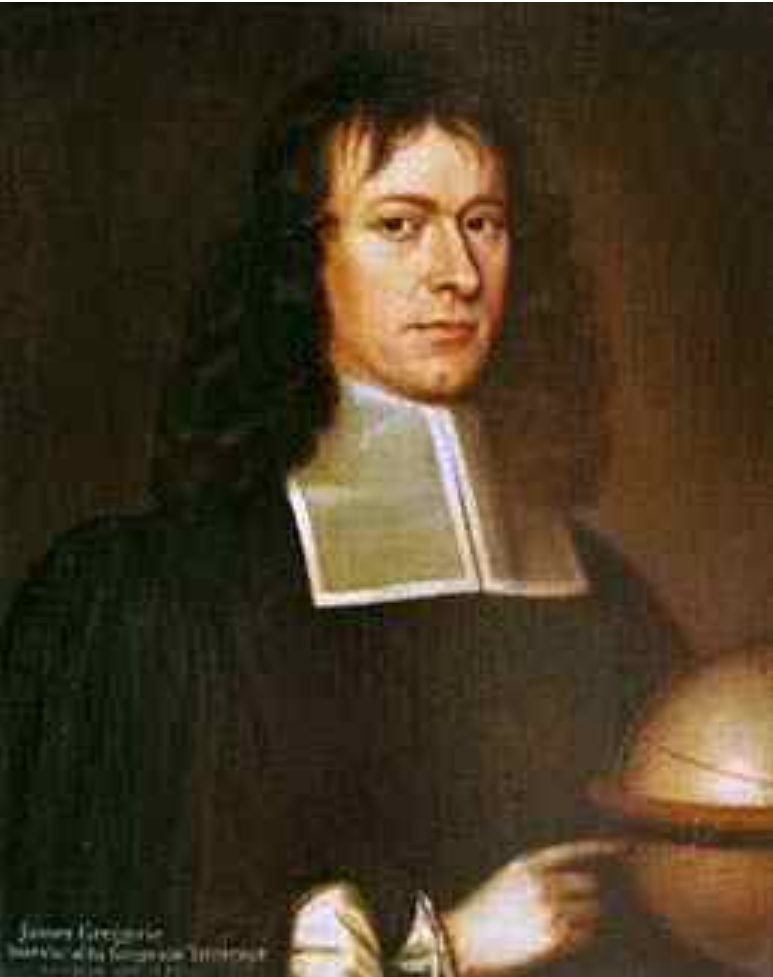
\includegraphics[width=\linewidth]{external/images/JamesGregory.png}
\end{image}%
\tcblower
\end{figureptx}%
\index{Newton, Isaac} Newton knew of these results and the general scheme of using power series to compute areas under curves. He used these results to provide a power series approximation for \(\pi\) as well, which, hopefully, would converge faster.  We will use modern terminology to streamline Newton's ideas.  First notice that \(\frac{\pi}{4}=\int_{x=0}^1\sqrt{1-x^2}\dx{ x}\) as this integral gives the area of one quarter of the unit circle, \(\frac{\pi }{4}\).  The trick now is to find a power series that represents \(\sqrt{1-x^2}\).%
\par
To this end we start with the binomial theorem%
\begin{equation*}
\left(a+b\right)^N=\sum_{n=0}^N\binom{N}{n}a^{N-n}b^n\text{,}
\end{equation*}
where%
\begin{align*}
\binom{N}{n}\amp =\frac{N!}{n!\left(N-n\right)!}\\
\amp =\frac{N\left(N-1\right)\left(N-2\right)\cdots\left(N-n+1\,\right)}{n!}\\
\amp =\frac{\prod_{j=0}^{n-1}\left(N-j\right)}{n!}\text{.}
\end{align*}
%
\par
Unfortunately, we now have a small problem with our notation which will be a source of confusion later if we don't fix it.  So we will pause to address this matter.  We will come back to the binomial expansion afterward.%
\par
This last expression is becoming awkward in much the same way that an expression like%
\begin{equation*}
1+\frac{1}{2}+\left(\frac{1}{2}\right)^2+\left(\frac{1}{2}\right)^3+\ldots+\left(\frac{1}{2}\right)^k
\end{equation*}
is awkward.  Just as this sum is less cumbersome when written as \(\sum_{n=0}^k\left(\frac{1}{2}\right)^n\) the \emph{product}%
\begin{equation*}
N\left(N-1\right)\left(N-2\right)\cdots\left(N-n+1\,\right)
\end{equation*}
is less cumbersome when we write it as \(\prod_{j=0}^{n-1}\left(N-j\right)\).%
\par
A capital pi \(\left(\Pi\right)\) is used to denote a product in the same way that a capital sigma \(\left(\Sigma\right)\) is used to denote a sum.  The most familiar example would be writing%
\begin{equation*}
n!=\prod_{j=1}^{n}j\text{.}
\end{equation*}
%
\par
Just as it is convenient to define \(0!=1\), we will find it convenient to define%
\begin{equation*}
\prod_{j=1}^{0}\left(\text{whatever}\right)=1\text{.}
\end{equation*}
Similarly, the fact that \(\binom{N}{0}=1\) leads to the convention \(\prod_{j=0}^{-1}\left(N-j\right)=1\). Strange as this may look, it is convenient and is consistent with the convention \(\sum_{j=0}^{-1}s_j=0\).%
\par
Returning to the binomial expansion and recalling our convention%
\begin{equation*}
\prod_{j=0}^{-1}\left(N-j\right)=1\text{,}
\end{equation*}
we can write,%
\begin{equation*}
\left(1+x\right)^N=1+\sum_{n=1}^N\left(\frac{\prod_{j=0}^{n-1}\left(N-j\right)}{n!}\right)x^n = \sum_{n=0}^N\left(\frac{\prod_{j=0}^{n-1}\left(N-j\right)}{n!}\right)x^n\text{.}
\end{equation*}
%
\par
These two representations may  look slightly different to you at first. Be sure that you see that they are really the same before reading further.%
\par
There is an advantage to using this convention (especially when programing a product into a computer), but this is not a deep mathematical insight.  It is just a notational convenience and we don't want you to fret over it, so we will use both formulations (at least initially).%
\par
Notice that we can extend the above definition of \(\binom{N}{n}\) to values \(n>N\).  In this case, \(\prod_{j=0}^{n-1}\left(N-j\right)\) will equal 0 as one of the factors in the product will be \(0\) (the one where \(j=N\)).  This gives us that \(\binom{N}{n}=0\) when \(n>N\) and so%
\begin{equation*}
\left(1+x\right)^N=1+\sum_{n=1}^\infty\left(\frac{\prod_{j=0}^{n-1}\left(N-j\right)}{n!}\text{ } \right)x^n= \sum_{n=0}^\infty\left(\frac{\prod_{j=0}^{n-1}\left(N-j\right)}{n!}\text{ } \right)x^n
\end{equation*}
holds true for any nonnegative integer \(N\). Essentially Newton asked if it could be possible that the above equation could hold values of \(N\) which are not nonnegative integers.  For example, if the equation held true for \(N=\frac{1}{2}\) , we would obtain%
\begin{equation*}
\left(1+x\right)^{\frac{1}{2}}=1+\sum_{n=1}^\infty\left(\frac{ \prod_{j=0}^{n-1}\left(\frac{1}{2}-j\right)}{n!}\right)x^n=\sum_{n=0}^\infty\left(\frac{ \prod_{j=0}^{n-1}\left(\frac{1}{2}-j\right)}{n!}\right)x^n
\end{equation*}
or%
\begin{equation}
\left(1+x\right)^{\frac{1}{2}}=1+\frac{1}{2}x+\frac{\frac{1}{2}\left(\frac{1}{2}-1\right)}{2!}x^2+\frac{\frac{1}{2}\left(\frac{1}{2}-1\right)\left(\frac{1}{2}-2\right)}{3!}x^3+\cdots\text{.}\label{eq_BinomialSeries}
\end{equation}
%
\par
Notice that since \(\frac{1}{2}\) is not an integer the power series no longer terminates.  Although Newton did not prove that this power series was correct (nor did we), he tested it by multiplying the power series by itself.  When he saw that by squaring the power series he started to obtain \(1+x+0\,x^2+0\,x^3+\cdots\), he was convinced that the power series was exactly equal to \(\sqrt{1+x}\).%
\begin{problem}{Problem}{}{ExponentAdditionProperty-55}%
Consider the power series representation%
\begin{align*}
\left(1+x\right)^{\frac{1}{2}}\amp =1+\sum_{n=1}^\infty\frac{\prod_{j=0}^{n-1}\left(\frac{1}{2}-j\right)}{n!}x^n\\
\amp  =\sum_{n=0}^\infty\frac{\prod_{j=0}^{n-1}\left(\frac{1}{2}-j\right)}{n!}x^n\text{.}
\end{align*}
%
\par
Multiply this power series by itself and compute the coefficients for \(x^0,\,x^1,\,x^2,\,x^3,\,x^4\) in the resulting power series.%
\end{problem}
\begin{problem}{Problem}{}{prob_SqrtSeriesProb}%
Let%
\begin{equation*}
S(x,M)=\sum_{n=0}^M\frac{\prod_{j=0}^{n-1}\left(\frac{1}{2}-j \right)}{n!}x^n\text{.}
\end{equation*}
%
\par
Use a computer algebra system to plot \(S(x,M)\) for \(M=5, 10, 15, 95, 100\) and compare these to the graph for \(\sqrt{1+x}\).  What seems to be happening?  For what values of \(x\) does the power series appear to converge to \(\sqrt{1+x}?\)%
\end{problem}
Convinced that he had the correct power series, Newton used it to find a power series representation of \(\int_{x=0}^1\sqrt{1-x^2}
\dx{ x}\).%
\begin{problem}{Problem}{}{ExponentAdditionProperty-58}%
Use the power series \(\displaystyle
\left(1+x\right)^{\frac{1}{2}}=\sum_{n=0}^\infty\frac{\prod_{j=0}^{n-1}\left(\frac{1}{2}-j\right)}{n!}x^n\) to obtain the power series%
\begin{align*}
\frac{\pi}{4}\amp =\int_{x=0}^1\sqrt{1-x^2} \dx{ x}\\
\amp =\sum_{n=0}^\infty\left[\left(\frac{\prod_{j=0}^{n-1}\left(\frac{1}{2}-j\right)}{n!}\text{ } \right)\left(\frac{\left(-1\right)^n}{2n+1}\right)\right]\\
\amp =1-\frac{1}{6}-\frac{1}{40}-\frac{1}{112}-\frac{5}{1152}-\cdots\text{.}
\end{align*}
%
\par
Use a computer algebra system to sum the first 100 terms of this power series and compare the answer to \(\frac{\pi}{4}\).%
\end{problem}
Again, Newton had a power series which could be verified (somewhat) computationally.  This convinced him even further that he had the correct power series.%
\begin{problem}{Problem}{}{ExponentAdditionProperty-60}%
%
\begin{enumerate}[label={(\alph*)}]
\item{}Show that%
\begin{equation*}
\int_{x=0}^{1/2}\sqrt{x-x^2}\dx{ x}=\sum_{n=0}^\infty\frac{(-1)^n\,\,\prod_{j=0}^{n-1}\left(\frac{1}{2}-j\right)}{\sqrt{2\,}n!\left(2n+3\right)2^n}
\end{equation*}
and use this to show that%
\begin{equation*}
\pi=16\left(\sum_{n=0}^\infty\frac{(-1)^n\,\,\prod_{j=0}^{n-1}\left(\frac{1}{2}-j\right)}{\sqrt{2\,}n!\left(2n+3\right)2^n}\right)\text{.}
\end{equation*}
%
\item{}We now have two power series for calculating \(\pi\): the one from part (a) and the one derived earlier, namely%
\begin{equation*}
\pi=4\left(\sum_{n=0}^\infty\frac{(-1)^n\,\,}{2n+1}\right)\text{.}
\end{equation*}
We will explore which one converges to \(\pi\) faster. First define%
\begin{equation*}
S1(N)=16\left(\sum_{n=0}^N\frac{(-1)^n\,\,\prod_{j=0}^{n-1}\left(
\frac{1}{2}-j\right)}{\sqrt{2\,}n!\left(2n+3\right)2^n}\right)
\end{equation*}
and%
\begin{equation*}
S2(N)=4\left(\sum_{n=0}^N\frac{(-1)^n\,\,}{2n+1}\right)\text{.}
\end{equation*}
Use a computer algebra system to compute \(S1(N)\)and \(S2(N)\) for \(N=5,10,15,20\).  Which one appears to converge to \(\pi\) faster?%
\end{enumerate}
%
\end{problem}
In general the power series representation%
\begin{align*}
\left(1+x\right)^\alpha \amp  =\sum_{n=0}^\infty\left(\frac{\prod_{j=0}^{n-1}\left(\alpha-j\right)}{n!}\text{ } \right)x^n\\
\amp =1+\alpha x+\frac{\alpha\left(\alpha-1\right)}{2!}x^2+\frac{\alpha\left(\alpha-1\right)\left(\alpha-2\right)}{3!}x^3+\cdots
\end{align*}
is called the \terminology{binomial series} (or Newton's binomial series).  This power series is correct when \(\alpha\) is a non-negative integer (after all, that is how we got the series in the first place).  We can also see that it is correct when \(\alpha=-1\) as we obtain%
\begin{align*}
\left(1+x\right)^{-1}\amp =\sum_{n=0}^\infty\left(\frac{\prod_{j=0}^{n-1}\left(-1-j\right)}{n!}\text{ } \right)x^n\\
\amp =1+(-1)x+\frac{-1\left(-1-1\right)}{2!}x^2+\frac{-1\left(-1-1\right)\left(-1-2\right)}{3!}x^3+\cdots\\
\amp =1-x+x^2-x^3+\cdots
\end{align*}
which can be obtained from the geometric series \(\frac{1}{1-x}=1+x+x^2+\cdots\) .%
\par
In fact, the binomial series is the correct power series representation for all values of the exponent \(\alpha\) (though we haven't proved this yet).%
\begin{problem}{Problem}{}{ExponentAdditionProperty-63}%
\begin{enumerate}[font=\bfseries,label=(\alph*),ref=\alph*]%
\item{}Assuming that the binomial series works for \(\alpha =-\frac{1}{2}\), show that%
\begin{align*}
\frac{1}{\sqrt{1-x^2}}\amp{}=\sum^{\infty}_{n=0}{\frac{\left(\prod^{n-1}_{j=0}{\left(\frac{1}{2}+j\right)}\right)}{n!}x^{2n}}\\
\amp{}
=1+\frac{1}{2}x^2+\frac{\left(\frac{1}{2}\right)\left(\frac{3}{2}\right)}{2!}x^4+\frac{\left(\frac{1}{2}\right)\left(\frac{3}{2}\right)\left(\frac{5}{2}\right)}{3!}x^6+\dots.
\end{align*}
%
\item{}Integrate the above to obtain the following power series for \(\arcsin (x)\).%
\begin{align*}
\arcsin \left(x\right)\amp{}=\sum^{\infty
}_{n=0}{\frac{\left(\prod^{n-1}_{j=0}{\left(\frac{1}{2}+j\right)}\right)}{n!\left(2n+1\right)}x^{2n+1}}\\
\amp{}=x+\frac{\frac{1}{2}}{3}x^3+\frac{\left(\frac{1}{2}\right)\left(\frac{3}{2}\right)}{2!5}x^5+\frac{\left(\frac{1}{2}\right)\left(\frac{3}{2}\right)\left(\frac{5}{2}\right)}{3!7}x^7+\dots 
\end{align*}
%
\item{}Substitute \(x=\frac{1}{2}\) into the above power series to obtain a power series representation for \(\frac{\pi
}{6}\).  Add the first four terms of this power series to obtain an approximation for \(\pi \), and compare with \(\pi
\approx 3.14159265359\).  How close did your approximation come?%
\end{enumerate}%
\end{problem}
\begin{problem}{Problem}{}{ExponentAdditionProperty-64}%
Let \(k\) be a positive integer.  Find the power series, centered at zero, for \(f(x) =
\left(1-x\right)^{-k}\) by%
\begin{enumerate}[font=\bfseries,label=(\alph*),ref=\alph*]%
\item{}Differentiating the \hyperref[EQUATIONGeometricSeries]{Geometric series} \(\left(k-1\right)\) times.%
\item{}Applying the binomial series.%
\item{}Compare the results in parts (a) and (b).%
\end{enumerate}%
\end{problem}
\href{https://mathshistory.st-andrews.ac.uk/Biographies/Euler/}{Leonhard Euler} (1707\textendash{}1783) was a master at exploiting power series.  In 1735, the 28 year-old Euler won acclaim for what is now called the Basel problem: to evaluate the sum%
\begin{equation*}
\sum_{n=1}^\infty\frac{1}{n^2}\text{.}
\end{equation*}
Other mathematicans had shown that the power series converged, but Euler was the first to find its exact value.  The following problem essentially provides Euler's solution.%
\begin{figureptx}{Figure}{Leonhard Euler}{ExponentAdditionProperty-66}{}%
\index{Euler, Leonhard!portrait of}%
\index{Portraits!Euler}%
\begin{image}{0.325}{0.35}{0.325}{}%
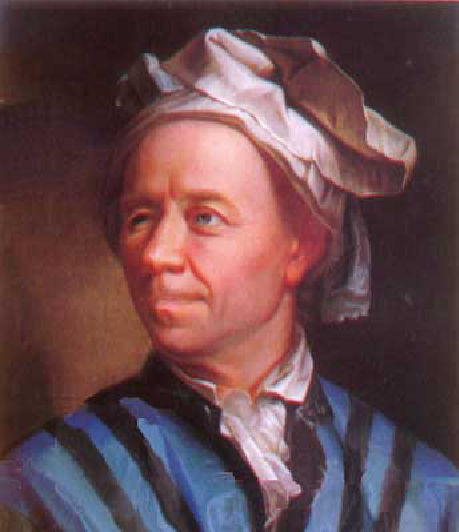
\includegraphics[width=\linewidth]{external/images/Euler.png}
\end{image}%
\tcblower
\end{figureptx}%
\begin{problem}{Problem}{The Basel Problem.}{ExponentAdditionProperty-67}%
Recall that in \hyperref[PROBLEMSinCosPwrSeries]{Problem~{\xreffont\ref{PROBLEMSinCosPwrSeries}}} we developed a power series representation of the function  \(\sin x\).%
\begin{enumerate}[font=\bfseries,label=(\alph*),ref=\alph*]%
\item{}Show that the power series for \(\frac{\sin x}{x}\) is given by \(1-\frac{1}{3!}x^2+\frac{1}{5!}x^4-\cdots\)%
\item{}Use part (a) to infer that the roots of \(1-\frac{1}{3!}x^2+\frac{1}{5!}x^4-\cdots\) are given by%
\begin{equation*}
x=\pm\pi,\,\pm 2\pi,\,\pm 3\pi,\,\ldots
\end{equation*}
%
\item{}Suppose \(p(x)=a_0+a_1x+\cdots+a_nx^n\) is a polynomial with roots \(r_1,\,r_2,\,\ldots,r_n\). Show that if \(a_0\neq\) \(0\), then all the roots are non-zero and%
\begin{equation*}
p(x)=a_0\left(1-\frac{x}{r_1}\right)\left(1-\frac{x}{r_2}\right)\cdots\left(1-\frac{x}{r_n}\right)\text{.}
\end{equation*}
%
\item{}Assuming that the result in part (c) holds for an infinite polynomial (power series), deduce that%
\begin{equation*}
1-\frac{1}{3!}x^2+\frac{1}{5!}x^4-\cdots =
\left(1-\left(\frac{x}{\pi}\right)^2\right)
\left(1-\left(\frac{x}{2\pi}\right)^2\right)
\left(1-\left(\frac{x}{3\pi}\right)^2\right)\cdots
\end{equation*}
%
\item{}Expand this product to deduce that%
\begin{equation*}
\sum_{n=1}^\infty\frac{1}{n^2}=\frac{\pi^2}{6}.{}
\end{equation*}
%
\end{enumerate}%
\end{problem}
\begin{problem}{Problem}{Euler's Formula.}{ExponentAdditionProperty-68}%
\begin{enumerate}[font=\bfseries,label=(\alph*),ref=\alph*]%
\item{}Use the power series expansion of \(e^x\), \(\sin
x,\) and \(\cos x\) to derive \terminology{Euler's Formula}:%
\begin{equation*}
e^{i\theta} = \cos\theta+i\sin\theta.
\end{equation*}
%
\item{}Use Euler's formula to derive the Addition\slash{}Subtraction formulas from Trigonometry:%
\begin{equation*}
\sin(\alpha\pm\beta) = \sin\alpha\cos\beta\pm\sin\beta\cos\alpha
\end{equation*}
%
\begin{equation*}
\cos(\alpha\pm\beta) = \cos\alpha\cos\beta\mp\sin\alpha\sin\beta
\end{equation*}
%
\item{}Use Euler's formula to show that%
\begin{equation*}
\sin 2\theta = 2\cos\theta\sin\theta
\end{equation*}
%
\begin{equation*}
\cos 2\theta =\cos^2\theta-\sin^2\theta
\end{equation*}
%
\item{}Use Euler's formula to show that%
\begin{equation*}
\sin 3\theta = 3\cos^2\theta\sin\theta-\sin^3\theta
\end{equation*}
%
\begin{equation*}
\cos 3\theta=\cos^3\theta-3\cos\theta\sin^2\theta
\end{equation*}
%
\item{}Find a formula \(\sin(n\theta)\) and \(\cos(n\theta)\) for any positive integer \(n\).%
\end{enumerate}%
\end{problem}
\end{sectionptx}
%
%
\typeout{************************************************}
\typeout{Section 3.3 Expanding Simple Power Series by Algebraic Methods}
\typeout{************************************************}
%
\begin{sectionptx}{Section}{Expanding Simple Power Series by Algebraic Methods}{}{Expanding Simple Power Series by Algebraic Methods}{}{}{SECTIONPowSerWOTaylor}
We call the power series expansions we'll see in this section ``simple'' because all that is needed to generate them is prior knowledge of a few series (e.g.,the \hyperref[EQUATIONGeometricSeries]{Geometric Series}, the \hyperref[PROBLEMSinCosPwrSeries]{sine and cosine series}, the \hyperref[EQUATIONExpSeries]{exponential series}, the \hyperref[eq_BinomialSeries]{Binomial Series}), and a creative use of algebra. In particular \hyperref[TaylorsTheorem]{Taylor's Theorem} is not needed. We assume that you are familiar with the use of Taylor's Theorem from your Calculus course.%
\par
As we saw in the last section, it can be particularly fruitful to expand a function as a power series centered at \(a=0\). Unfortunately, this isn't always possible. For example, it is not possible to expand the function \(f\left(x\right)=\frac{1}{x}\) about zero. (Why not?)%
\par
But we are not confined to expanding about zero.  Consider that the following is a power series for \(f(x)=\frac{1}{x}\) expanded about \(a=1\)%
\begin{equation*}
\frac{1}{x}=\frac{1}{1+\left(x-1\right)}=\sum^{\infty}_{n=0}{-1^n{\left(x-1\right)}^n}\text{.}
\end{equation*}
Of course, there are still questions that need to be resolved. Chief among these is the question, ``For which values of \(x\) is this series a valid representation of the function we started with?'' We will explore this in \hyperref[PowerSeriesQuestions-TaylorsFormula]{Section~{\xreffont\ref{PowerSeriesQuestions-TaylorsFormula}}}. For now we will content ourselves with having a representation which seems reasonable.%
\begin{problem}{Problem}{}{PROBLEMOneOverXTayl}%
Let \(a\neq 0\).%
\begin{enumerate}[font=\bfseries,label=(\alph*),ref=\alph*]%
\item{}Represent \(\frac{1}{x}\) as a power series expanded about \(a\).  That is, as a power series of the form \(\sum^{\infty }_{n=0}{a_n{(x-a)}^n}\).%
\par\smallskip%
\noindent\textbf{\blocktitlefont Hint}.\hypertarget{PROBLEMOneOverXTayl-2-2}{}\quad{}\(\frac{1}{x}=\frac{1}{a+x-a}=\frac{1}{a}\left(\frac{1}{1+\frac{x-a}{a}}\right)\)%
\item{}Represent \(\ln (x)\) as a power series expanded about \(a\) by integrating your solution to part (a).%
\end{enumerate}%
\end{problem}
\begin{problem}{Problem}{}{SECTIONPowSerWOTaylor-6}%
Let \(a>0\) and use \hyperref[eq_BinomialSeries]{equation~({\xreffont\ref{eq_BinomialSeries}})} to represent \(\sqrt{x}\) as a power series expanded about \(a\).%
\end{problem}
\begin{problem}{Problem}{}{PROBLEMExpTaylAta}%
Let \(a\) be a real number.  Represent \(e^x\) as power series expanded about \(a\).  Notice there is no restriction on \(a\).%
\end{problem}
\begin{problem}{Problem}{}{SECTIONPowSerWOTaylor-8}%
Let \(a\) be a real number.  Represent \(x^3+2x^2+3\) as a power series expanded about \(a\).  What happens if \(a=0\)?%
\end{problem}
\begin{problem}{Problem}{}{PROBLEMSinExpandedAta}%
Let \(a\) be a real number.  Use the power series expansions%
\begin{align*}
\sin \left(x\right)=\sum^{\infty
}_{n=0}{\frac{{\left(-1\right)}^n}{\left(2n+1\right)!}x^{2n+1}}\amp{}\amp{} \cos\left(x\right)=\sum^{\infty
}_{n=0}{\frac{{\left(-1\right)}^n}{\left(2n\right)!}x^{2n}}
\end{align*}
to obtain the power series representation%
\begin{align*}
\sin (x)=\sin (a)+\amp{}\cos \left(a\right)\left(x-a\right)-\frac{1}{2!}\sin
\left(a\right){\left(x-a\right)}^2\\
\amp{}-\frac{1}{3!}\cos
\left(a\right){\left(x-a\right)}^3+\frac{1}{4!}\sin
\left(a\right){\left(x-a\right)}^4\\
\amp{}\ \ \ \ \ +\frac{1}{5!}\cos
\left(a\right){\left(x-a\right)}^5+\cdots.
\end{align*}
%
\par
This result will come into play in the next section.%
\par\smallskip%
\noindent\textbf{\blocktitlefont Hint}.\hypertarget{PROBLEMSinExpandedAta-2}{}\quad{}\(\sin \left(x\right) =\sin \left(a+\left(x-a\right)\right)\)%
\end{problem}
\end{sectionptx}
\end{chapterptx}
%
%
\typeout{************************************************}
\typeout{Chapter 4 Questions Concerning Power Series}
\typeout{************************************************}
%
\begin{chapterptx}{Chapter}{Questions Concerning Power Series}{}{Questions Concerning Power Series}{}{}{PowerSeriesQuestions}
\renewcommand*{\chaptername}{Chapter}
%
%
\typeout{************************************************}
\typeout{Section 4.1 Taylor's Formula}
\typeout{************************************************}
%
\begin{sectionptx}{Section}{Taylor's Formula}{}{Taylor's Formula}{}{}{PowerSeriesQuestions-TaylorsFormula}
As we saw in \hyperref[SECTIONPowSerWOTaylor]{Section~{\xreffont\ref{SECTIONPowSerWOTaylor}}}, representing functions as power series was a fruitful strategy for mathematicans in the eighteenth century (as it still is). Differentiating and integrating power series term by term was relatively easy, \emph{seemed} to work, and led to many applications.  Furthermore, power series representations for all of the elementary functions could be obtained if one was clever enough. However, cleverness is an unreliable tool.  It would be better to have some systematic way to find a power series for a given function that doesn't rely on being sufficiently clever.%
\par
To be sure, there were nagging questions. For example. even if we can find a power series representation of some function, how do we know that the series we've created represents the function we started with?  Even worse, is it possible for a function to have more than one power series representation centered at a given value \(a?\) This uniqueness issue is addressed by the following theorem.%
\begin{theorem}{Theorem}{Taylor's Formula.}{}{THEOREMTaylorPoly}%
\index{Taylor's Formula}%
If \(f(x)=\sum_{n=0}^\infty a_n(x-a)^n\), then \(a_n=\frac{f^{(n)}(a)}{n!}\), where \(f^{(n)}(a)\) represents the \(n\)th derivative of \(f\) evaluated at \(a\).%
\end{theorem}
A few comments about \hyperref[THEOREMTaylorPoly]{Theorem~{\xreffont\ref{THEOREMTaylorPoly}}} are in order.  Notice that we did \emph{not} start with a function and derive its series representation.  Instead we \emph{defined} \(f(x)\) to be the series we wrote down.  This assumes that the expression \(\sum_{n=0}^\infty a_n(x-a)^n\) actually has meaning (that it converges).  At this point we have every reason to expect that it does, however expectation is not proof so we note that this is an assumption, not an established truth.  We've also assumed that we can differentiate an infinite polynomial term-by-term as we would a finite polynomial.  As before, we follow in the footsteps of our 18th century forebears in making these assumptions.  For now.%
\begin{problem}{Problem}{}{PowerSeriesQuestions-TaylorsFormula-6}%
Prove \hyperref[THEOREMTaylorPoly]{Theorem~{\xreffont\ref{THEOREMTaylorPoly}}}.%
\par\smallskip%
\noindent\textbf{\blocktitlefont Hint}.\hypertarget{PowerSeriesQuestions-TaylorsFormula-6-3}{}\quad{}The ``zeroth'' derivative (the function itself) at \(a\) is given by%
\begin{equation*}
f(a)=a_0+a_1(a-a)+a_2(a-a)^2+\cdots=a_0\text{.}
\end{equation*}
Differentiate to obtain the other terms.%
\end{problem}
From \hyperref[THEOREMTaylorPoly]{Theorem~{\xreffont\ref{THEOREMTaylorPoly}}} we see that if we do start with the function \(f(x)\) then no matter how we obtain its power series, the result will always be the same.  The series%
\begin{align}
\sum_{n=0}^\infty\frac{f^{(n)}(a)}{n!}(x-a)^n=f(a)+\amp{}f^\prime(a)(x-a)+\frac{f^{\prime\prime}(a)}{2!}(x-a)^2\notag\\
\amp{}+\frac{f^{\prime\prime\prime}(a)}{3!}(x-a)^3+\cdots\label{TaylorsSeries}
\end{align}
%
\par
is called the \emph{\alert{Taylor series} for \(f\) expanded about (or centered at) \(a\)}.  Although this systematic ``machine'' for obtaining power series for a function seems to have been known to a number of mathematicians in the early 1700s, \href{https://mathshistory.st-andrews.ac.uk/Biographies/Taylor/}{Brook Taylor} (1685\textendash{}1731) was the first to publish this result in his \textit{Methodus Incrementorum} (1715). The special case when \(a=0\) was included by \href{https://mathshistory.st-andrews.ac.uk/Biographies/Maclaurin/}{Colin Maclaurin} (1698\textendash{}1746) in his \emph{Treatise of Fluxions} (1742). Thus when \(a=0\), the series \(\sum_{n=0}^\infty\frac{f^{(n)}(0)}{n!}x^n\) is often called the \terminology{Maclaurin Series} for \(f\).%
\begin{figureptx}{Figure}{A postage stamp from the Netherlands honoring Brook  Taylor and Colin Maclaurin}{PowerSeriesQuestions-TaylorsFormula-9}{}%
\index{Taylor, Brook!portrait of}%
\index{Maclaurin, Colin!portrait of}%
\index{Portraits!Taylor}%
\index{Portraits!Maclaurin}%
\begin{image}{0.275}{0.45}{0.275}{}%
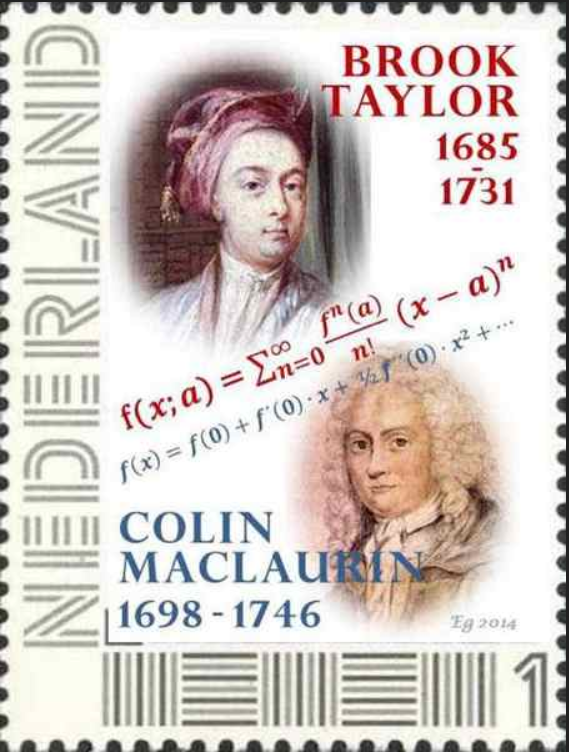
\includegraphics[width=\linewidth]{external/images/TaylorAndMaclaurin.png}
\end{image}%
\tcblower
\end{figureptx}%
\begin{problem}{Problem}{}{PowerSeriesQuestions-TaylorsFormula-10}%
Use \hyperref[THEOREMTaylorPoly]{Taylor's formula} to find the Taylor series of the given function expanded about the given point \(a\).%
\begin{enumerate}[font=\bfseries,label=(\alph*),ref=\alph*]%
\item{}\(f(x)=\ln\left(1+x\right)\), \(a=0\)%
\item{}\(f(x)=e^x\), \(a=-1\)%
\item{}\(f(x)=\sin(x) \), \(a=\frac{\pi }{2}\)%
\item{}\(f(x)=x^3+x^2+x+1\), \(a=0\)%
\item{}\(f(x)=x^3+x^2+x+1\), \(a=1\)%
\end{enumerate}%
\end{problem}
The \terminology{prime notation} for the derivative was not used by Taylor, Maclaurin or their contemporaries.  It was introduced by Joseph Louis Lagrange in his 1779 work \textit{Thèorie des Fonctions Analytiques}. In that work, Lagrange sought to get rid of Leibniz' infinitesimals and base Calculus on the power series idea.  His idea was that by representing every function as a power series, Calculus could be done algebraically by manipulating power series and examining various aspects of the series representation instead of appealing to the controversial notion of infinitesimals.  He implicitly assumed that every continuous function could be replaced with its power series representation.%
\begin{figureptx}{Figure}{\href{https://mathshistory.st-andrews.ac.uk/Biographies/Lagrange/}{Joseph-Louis Lagrange}}{PowerSeriesQuestions-TaylorsFormula-12}{}%
\index{Lagrange, Joseph-Louis!portrait of}%
\index{Portraits!Lagrange}%
\begin{image}{0.325}{0.35}{0.325}{}%
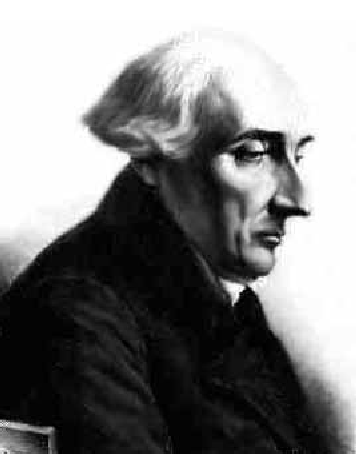
\includegraphics[width=\linewidth]{external/images/Lagrange.png}
\end{image}%
\tcblower
\end{figureptx}%
That is, he wanted to think of the Taylor series as a ``great big polynomial,'' because polynomials are easy to work with. It was a very simple, yet exceedingly clever and far-reaching idea. Since \(e^x = 1 +x +x^2/2 +\ldots\), for example, why not just define the exponential to be the series and work with the series. After all, the series is just a very long polynomial.%
\par
This idea did not come out of nowhere. Particular infinite series, such as the \hyperref[EQUATIONGeometricSeries]{Geometric Series} had been known and studied for many years.  Later, in the 18th century Leonhard Euler used infinite series to solve many problems, and some of his solutions are still quite breath\textendash{}taking when you first see them~\hyperlink{sandifer07__early_mathem_leonar_euler}{[{\xreffont 14}]}.%
\par
Taking his cue from the Taylor series%
\begin{equation}
f(x) = \sum_{n=0}^\infty\frac{f^{(n)}(a)}{n!}(x-a)^n\label{EQUATIONTaylorSeriesGeneric}
\end{equation}
Lagrange observed that the coefficient of \((x-a)^n\) provides the \(n\)th derivative of \(f\) at \(a\) (divided by \(n!\)). Modifying \hyperref[EQUATIONTaylorSeriesGeneric]{formula~({\xreffont\ref{EQUATIONTaylorSeriesGeneric}})} to suit his purpose, Lagrange supposed that every differentiable function could be represented as%
\begin{equation*}
f(x) = \sum_{n=0}^\infty g_n(a)(x-a)^n\text{.}
\end{equation*}
%
\par
In that case \(g_1(a)\) is the derivative of \(f\) at \(a\), \(f^{\prime\prime}(a)=2g_2(a)\) and generally%
\begin{equation*}
f^{(n)}(a)=n! g_n(a)\text{.}
\end{equation*}
%
\par
Lagrange dubbed his function \(g_1\) the \textit{``fonction dérivée''} from which we get the modern name \terminology{derivative}.%
\begin{problem}{Problem}{}{PowerSeriesQuestions-TaylorsFormula-18}%
Let \(a\neq 0\) be a fixed number. We saw in \hyperref[PROBLEMOneOverXTayl]{Problem~{\xreffont\ref{PROBLEMOneOverXTayl}}}  that the power series of \(\frac{1}{x}\) expanded about \(a\) is given by%
\begin{equation*}
\sum^{\infty}_{n=0}{\frac{{\left(-1\right)}^n}{a^{n+1}}{\left(x-a\right)}^n}
=\frac{1}{a}-\frac{1}{a^2}\left(x-a\right)
+\frac{1}{a^3}{\left(x-a\right)}^2
-\frac{1}{a^4}{\left(x-a\right)}^3+\dots
\end{equation*}
%
\begin{enumerate}[font=\bfseries,label=(\alph*),ref=\alph*]%
\item{}Apply Lagrange's idea to show that \(f^{\left(n\right)}\left(a\right)=\frac{{\left(-1\right)}^nn!}{a^{n+1}}\).%
\item{}Now compute \(f^{\left(n\right)}\left(a\right)\) by directly by differentiating.  Do you get the same result?%
\end{enumerate}%
\end{problem}
\begin{problem}{Problem}{}{PowerSeriesQuestions-TaylorsFormula-19}%
\begin{enumerate}[font=\bfseries,label=(\alph*),ref=\alph*]%
\item{}In \hyperref[PROBLEMSinExpandedAta]{Problem~{\xreffont\ref{PROBLEMSinExpandedAta}}}, you determined the power series expansion%
\begin{align*}
\sin (x)=\sin (a)+\amp{}\cos\left(a\right)\left(x-a\right)\\
\amp{}-\frac{1}{2!}\sin
\left(a\right){\left(x-a\right)}^2\\
\amp{}\ \ \ -\frac{1}{3!}\cos
\left(a\right){\left(x-a\right)}^3\\
\amp{}\ \ \ \ \ \ +\frac{1}{4!}\sin
\left(a\right){\left(x-a\right)}^4\\
\amp{}\ \ \ \ \ \ \ \ \  +\frac{1}{5!}\cos
\left(a\right){\left(x-a\right)}^5+\cdots.
\end{align*}
%
\par
Apply Lagrange's idea to determine the \(n\)th derivative of \(\sin x\). Compare with the results you get from differentiating \(\sin x\) directly.%
\item{}In \hyperref[PROBLEMExpTaylAta]{Problem~{\xreffont\ref{PROBLEMExpTaylAta}}} you determined the power series expansion of \(e^x\) about \(a\).  Apply Lagrange's idea to show that every derivative of \(e^x\) is given by \(e^x\).%
\item{}In part (b) of \hyperref[PROBLEMOneOverXTayl]{Problem~{\xreffont\ref{PROBLEMOneOverXTayl}}} you determined the power series expansion of \(\ln(x)\) about \(a>0\). Apply Lagrange's idea to show that the derivative of \(\ln (x)\) is \(\frac{1}{x}\).%
\end{enumerate}%
\end{problem}
As we observed in \hyperref[CalcIn17th18thCentury-NewtLeibStart]{Section~{\xreffont\ref{CalcIn17th18thCentury-NewtLeibStart}}} Leibniz and his peers would have regarded the expression \(\dfdx{z}{x}\) as a fraction (of differentials) so they would have derived the formula%
\begin{equation}
\dfdx{z}{y}\dfdx{y}{x}=\dfdx{z}{x}\label{EQUATIONChainRuleLeibniz}
\end{equation}
by simply canceling the \(\dx{y}\) that appears in the numerator and denominator, just as we did in \hyperref[CalcIn17th18thCentury-NewtLeibStart]{Section~{\xreffont\ref{CalcIn17th18thCentury-NewtLeibStart}}} (or sometimes by ``uncancelling'' them to get the left side of \hyperref[EQUATIONChainRuleLeibniz]{equation~({\xreffont\ref{EQUATIONChainRuleLeibniz}})} from the right side).  Mathematicians of that era would have regarded this operation as basic algebra.%
\par
Eighteenth and nineteenth century arithmetic primers used the phrase ``chain rule'' to describe the daisy\textendash{}chain of symbolic cancellations that occurs when we convert units. For example, to convert yards to inches we compute%
\begin{equation*}
\left(2\cancel{\text{ yards}}\right)\left(3\frac{\cancel{\text{feet}}}{\cancel{\text{yard}}}\right)\left(12\frac{\text{inches}}{\cancel{\text{foot}}}\right)=72\text{ inches}\text{.}
\end{equation*}
%
\par
Since the cancellations in \hyperref[EQUATIONChainRuleLeibniz]{equation~({\xreffont\ref{EQUATIONChainRuleLeibniz}})} appeared to be just another example of the older ``chain rule'' the name was adopted by 20th century Calculus textbooks even though in modern times it is better understood as a mnemonic for the deeper and more abstract operation of computing the derivative of composed functions like \(f(g(x))\).%
\par
Letting \(z=f(y)\) and \(y=g(x)\) and using Lagrange's prime notation we see that in modern form the chain rule for Calculus is:%
\begin{equation*}
\dfdx{z}{x}=\left(f\circ
g\right)^\prime\left(x\right)=\underbrace{f^\prime\left(g\left(x\right)\right)}_{\dfdx{z}{y}}\underbrace{g^\prime(x)}_{\dfdx{y}{x}{}}\text{.}
\end{equation*}
Which obviously looks nothing like the older chain rule seen as in \hyperref[EQUATIONChainRuleLeibniz]{equation~({\xreffont\ref{EQUATIONChainRuleLeibniz}})}%
\par
In his \textit{Théorie des  fonctions analytiques} (1797) Lagrange  provided a derivation of the Chain Rule in these more modern terms.   The following problem captures his idea.%
\begin{problem}{Problem}{}{PowerSeriesQuestions-TaylorsFormula-25}%
%
\begin{enumerate}[font=\bfseries,label=(\alph*),ref=\alph*]%
\item{}Expand \(y=g(x)\) as a power series expanded about \(a\).%
\item{}Expand \(f(y)\) as a power series expanded about \(y=g(a)\) and substitute your answer from part (a) for \(y\).%
\item{}Show that the coefficient of the linear term \((x-a)\) in part (b) is given by%
\begin{equation*}
f^\prime\left(g\left(a\right)\right)g^\prime(a)
\end{equation*}
%
\end{enumerate}%
\end{problem}
All in all, Lagrange's idea was very clever and insightful. It's only real flaw is that the fundamental, underlying assumption is not true.  It turns out that not every differentiable function can be represented as a Taylor series. This was demonstrated very dramatically by Augustin Cauchy's famous counter-example%
\begin{equation}
f(x) = \begin{cases} e^{-\frac{1}{x^2}}\amp  x\ne0\\ 0 \amp x=0 \end{cases}\text{.}\label{eq_CauchyCounterEx}
\end{equation}
%
\par
This function is actually infinitely differentiable everywhere but its Maclaurin series (that is, its Taylor series with \(a=0\)) does not converge to \(f\) (except, trivially, at the origin) because all of its derivatives at the origin are equal to zero. That is \(f^{(n)}(0) = 0, \forall\, n \in
\NN\).%
\par
To begin with, let's compute a few derivatives when \(x
\neq 0\).%
\begin{align*}
f^{(0)}(x) \amp = e^{x^{-2}}\\
f^{(1)}(x) \amp = 2x^{-3}e^{-x^{-2}}\\
f^{(2)}(x) \amp = \left(4x^{-6}-6x^{-4}\right)e^{-x^{-2}}\text{.}
\end{align*}
%
\par
As you can see the calculations are already getting a little complicated and we've only taken the second derivative.%
\par
Conceptually, it is not difficult to compute these derivatives using the tools you learned in Calculus but the formulas involved do become complicated rather quickly.  Some care must be taken to avoid error. To streamline things a bit we take \(y= x^{-1}\), and define \(p_2(x) = 4x^6-6x^4\) so that%
\begin{equation*}
f^{(2)}(x) = p_2(x^{-1})e^{-x^{-2}} = p_2(y)e^{-y^2}\text{.}
\end{equation*}
%
\begin{problem}{Problem}{Cauchy's Counterexample, Part 1.}{DRILLCauchyCounterPartI}%
In this problem and in \hyperref[PROBLEMCauchyCounterPartII]{Problem~{\xreffont\ref{PROBLEMCauchyCounterPartII}}} \(f(x)\) is the function defined in \hyperref[eq_CauchyCounterEx]{equation~({\xreffont\ref{eq_CauchyCounterEx}})}.%
 \par
To simplify the notation we make the following definitions: \(y=x^{-1}\) and \(f^{(n)}(x) =p_n(y)e^{-y^2}\).%
\begin{enumerate}[font=\bfseries,label=(\alph*),ref=\alph*]%
\item{}Find \(p_{n+1}(y)\) in terms of \(p_{n}(y)\).%
\par\smallskip%
\noindent\textbf{\blocktitlefont Hint}.\hypertarget{DRILLCauchyCounterPartI-4-2}{}\quad{}You are differentiating with respect to \(x\), not \(y\).%
\item{}Use induction on \(n\) to show that \(p_n(y)\) is a polynomial for all \(n\in\NN\).%
\end{enumerate}%
\end{problem}
Unfortunately everything we've done so far only gives us the derivatives we need when \(x\) is \emph{not} zero, and we need the derivatives when \(x\) \emph{is} zero. To find these we need to get back to very basic ideas.%
\par
Let's assume for the moment that we know that \(f^{(n)}(0)=0\) and recall that%
\begin{align*}
f^{(n+1)}(0) \amp = \limit{x}{0}{\frac{f^{(n)}(x)-f^{(n)}(0)}{x-0}}\\
f^{(n+1)}(0) \amp = \limit{x}{0}{x^{-1}p_n(x^{-1})e^{-x^{-2}}}\\
f^{(n+1)}(0) \amp = \limit{y}{\pm\infty}{\frac{yp_n(y)}{e^{y^2}}}\text{.}
\end{align*}
%
\par
We can close the deal with the following problem.%
\begin{problem}{Problem}{Cauchy's Counterexample, Part 2.}{PROBLEMCauchyCounterPartII}%
\begin{enumerate}[font=\bfseries,label=(\alph*),ref=\alph*]%
\item{}Let \(m\) be a nonnegative integer. Show that \(\limit{y}{\pm\infty}{\frac{y^m}{e^{y^2}}}=0\).%
\par\smallskip%
\noindent\textbf{\blocktitlefont Hint}.\hypertarget{PROBLEMCauchyCounterPartII-3-2}{}\quad{}Induction and a dash of L'Hôpital's rule should do the trick.%
\item{}Prove that \(\limit{y}{\pm\infty}{\frac{q(y)}{e^{y^2}}}=0\) for any polynomial \(q\).%
\item{}Let \(f(x)\) be as in \hyperref[eq_CauchyCounterEx]{equation~({\xreffont\ref{eq_CauchyCounterEx}})} and show that for every nonnegative integer \(n\), \(f^{(n)}(0)=0\).%
\end{enumerate}%
\end{problem}
This example showed that while it was fruitful to exploit Taylor series representations of various functions, basing the foundations of Calculus on power series was not a sound idea.%
\par
While Lagrange's approach wasn't totally successful, it was a major step away from infinitesimals and toward the modern approach.  We still use aspects of it today.  For instance we still use his prime notation to denote the derivative.%
\par
Turning Lagrange's idea on its head it is clear that if we know how to compute derivatives, we can use this ``machine'' to obtain a power series when we are not clever enough to obtain the series by other (typically shorter) means.  For example, consider Newton's binomial series when \(\alpha=\frac{1}{2}\).  Originally, we obtained this series by extending the binomial theorem to non-integer exponents. Taylor's formula provides a more systematic procedure. First we compute the derivatives of \(f\) at zero:%
\begin{align*}
f(x)\amp =(1+x)^{\frac{1}{2}};\amp f(0)\amp =1\\
f^\prime(x)\amp =\frac{1}{2}(1+x)^{\frac{1}{2}-1};\amp  f^\prime(0)\amp =\frac{1}{2}\\
f^{\prime\prime}(x)\amp =\frac{1}{2}\left(\frac{1}{2}-1\right)(1+x)^{\frac{1}{2}-2}\amp f^{\prime\prime}(0)\amp =\frac{1}{2}\left(\frac{1}{2}-1\right)
\end{align*}
and in general since%
\begin{align*}
f^{(n)}(x)\amp =\frac{1}{2}\left(\frac{1}{2}-1\right)\cdots\left(\frac{1}{2}-(n-1)\right)(1+x)^{\frac{1}{2}-n}\\
\intertext{we have}
f^{(n)}(0)\amp =\frac{1}{2}\left(\frac{1}{2}-1\right)\cdots\left(\frac{1}{2}-(n-1)\right)\text{.}
\end{align*}
%
\par
Next we substitute  \(f^{(n)}(0)\) into  Taylor's formula to obtain the series%
\begin{align*}
\sum_{n=0}^\infty\frac{f^{(n)}(0)}{n!}x^n \amp{}= 1+\sum_{n=1}^\infty\frac{\frac{1}{2}\left(\frac{1}{2}-1\right)\cdots\left( \frac{1}{2}-(n-1)\right)}{n!}x^n\\
\amp{}= 1+\sum_{n=1}^\infty\frac{\prod_{j=0}^{n-1}\left(\frac{1}{2}-j\right)}{n!}x^n
\end{align*}
which agrees with \hyperref[eq_BinomialSeries]{equation~({\xreffont\ref{eq_BinomialSeries}})} in the previous chapter.%
\begin{problem}{Problem}{}{PowerSeriesQuestions-TaylorsFormula-40}%
Use Taylor's formula to obtain the general binomial series%
\begin{equation*}
(1+x)^\alpha=1+\sum_{n=1}^\infty\frac{\prod_{j=0}^{n-1}\left(\alpha-j\right)}{n!}x^n.{}
\end{equation*}
%
\end{problem}
As you can see, Taylor's ``machine'' will produce the power series for a function (if it has one), but is tedious to perform.  We will find, generally, that this tediousness can be an obstacle to understanding.  In many cases it will be better, or at least quicker, to be clever if we can.  However, it is comforting to have Taylor's formula available as a last resort.%
\par
The existence of a Taylor series is addressed (to some degree) by the following.%
\begin{theorem}{Theorem}{Taylor's Theorem.}{}{TaylorsTheorem}%
\index{Taylor's Theorem}%
If \(f^\prime, f^{\prime\prime}, \ldots, f^{(n+1)}\) are all continuous on an interval containing \(a\) and \(x\), then%
\begin{align*}
f(x)=f(a)+\amp{}\frac{f^{\prime}(a)}{1!}(x-a)+\frac{f^{\prime \prime}(a)}{2!}(x-a)^2 +\\
\amp{}\cdots+\frac{f^{(n)}(a)}{n!}(x-a)^n + \frac{1}{n!}\int_{t=a}^xf^{(n+1)}(t)(x-t)^n\dx{t}\text{.}
\end{align*}
The last term in this expression,%
\begin{equation*}
\frac{1}{n!}\int_{t=a}^xf^{(n+1)}(t)(x-t)^n\dx{t}\text{,}
\end{equation*}
is called the \terminology{Integral Form of the Remainder} of the Taylor series.%
\end{theorem}
The proof of \hyperref[TaylorsTheorem]{Theorem~{\xreffont\ref{TaylorsTheorem}}} will be by \terminology{Mathematical Induction} but before we address the proof, notice that the \(n\)th degree polynomial%
\begin{equation}
f(a)+\frac{f^{\prime}(a)}{1!}(x-a)+\frac{f^{\,\prime\prime}(a)}{2!}(x-a)^2+\cdots+\frac{f^{(n)}(a)}{n!}(x-a)^n\label{EQUATIONNthDegTaylPoly}
\end{equation}
resembles the Taylor series and, in fact, is called the \terminology{\(\boldsymbol n\)th degree Taylor polynomial of \(f\) about \(\boldsymbol a\)}.  \hyperref[TaylorsTheorem]{Theorem~{\xreffont\ref{TaylorsTheorem}}} says that a function can be written as the sum of this polynomial and a specific integral which we will analyze in \hyperref[TaylorSeries]{Chapter~{\xreffont\ref{TaylorSeries}}}.%
\par
We will get the proof started and leave the formal induction proof as an exercise. To begin the induction notice that when \(n=0\) \hyperref[EQUATIONNthDegTaylPoly]{equation~({\xreffont\ref{EQUATIONNthDegTaylPoly}})} is  a restatement of the \terminology{Fundamental Theorem of Calculus}:%
\begin{equation*}
\int_{t=a}^xf^\prime(t)\dx{t}=f(x)-f(a)\text{.}
\end{equation*}
which we rewrite  as%
\begin{equation*}
f(x)=f(a)+\frac{1}{0!}\int_{t=a}^xf^\prime(t)(x-t)^0\dx{t}
\end{equation*}
in order to provide the anchor step (when \(n=0\)) for our induction.%
\begin{aside}{Aside}{The Fundamental Theorem of Calculus.}{PowerSeriesQuestions-TaylorsFormula-46}%
Strictly speaking, this proof will not be complete until we prove the \terminology{Fundamental Theorem of Calculus} in \hyperref[SECTIONFTC]{Section~{\xreffont\ref{SECTIONFTC}}}, but you should be familiar with it from your Calculus course.%
\end{aside}
To derive the case where \(n=1\), we use integration by parts. If we let%
\begin{align*}
u\amp =f^\prime(t)\amp  d v\amp =(x-t)^0d t\\
d u\amp =f^{\prime\prime}(t)d t\amp  v\amp =-\frac{1}{1}(x-t)^1
\end{align*}
we obtain%
\begin{align*}
f(x)\amp =f(a)+\frac{1}{0!}\left(-\frac{1}{1}f^\prime(t)(x-t)^1|_{t=a}^{^x}+\frac{1}{1} \int_{t=a}^xf^{\prime\prime}(t)(x-t)^1\dx{ t}\right)\\
\amp =f(a)+\frac{1}{0!}\left(-\frac{1}{1}f^\prime(x)(x-x)^1+ \frac{1}{1}f^\prime(a)(x-a)^1+\frac{1}{1}\int_{t=a}^xf^{\prime\prime}(t)(x-t)^1\dx{ t}\right)\\
\amp =f(a)+\frac{1}{1!}f^\prime(a)\left(x-a\right)^1 + \frac{1}{1!}\int_{t=a}^xf^{\prime\prime}(t)(x-t)^1\dx{ t}\text{.}
\end{align*}
%
\begin{problem}{Problem}{}{PowerSeriesQuestions-TaylorsFormula-48}%
Provide a formal induction proof for \hyperref[TaylorsTheorem]{Theorem~{\xreffont\ref{TaylorsTheorem}}}.%
\end{problem}
\end{sectionptx}
%
%
\typeout{************************************************}
\typeout{Section 4.2 Series Anomalies}
\typeout{************************************************}
%
\begin{sectionptx}{Section}{Series Anomalies}{}{Series Anomalies}{}{}{PowerSeriesQuestions-SeriesAnomalies}
Until we began this chapter our approach to series mirrored that of the eighteenth century mathematicians. By exploiting the ideas of Calculus and power series they ingeniously derived mathematical results which were virtually unobtainable before. Mathematicans were eager to push these techniques as far as they could to obtain their results and they often showed good intuition regarding what was mathematically acceptable and what was not.  However, as the envelope was pushed further and further, substantial questions about the validity of their methods surfaced.%
\par
As an illustration consider the series expansion%
\begin{equation*}
\frac{1}{1+x}=1-x+x^2-x^3+\cdots\text{.}
\end{equation*}
%
\par
If we substitute \(x=1\) into this equation, we obtain%
\begin{equation*}
\frac{1}{2}=1-1+1-1+\cdots\text{.}
\end{equation*}
%
\par
If we group the terms as follows \((1-1)+(1-1)+\cdots\), the series would equal \(0\).  A regrouping of \(1+(-1+1)+(-1+1)+\cdots\) provides an answer of \(1\). This violation of the associative law of addition did not escape the mathematicians of the 1700s.  In his 1760 paper \pubtitle{On Divergent Series} Euler said:%
\begin{quote}%
\index{Leibniz, Gottfried Wilhelm} Notable enough, however are the controversies over the series \(1-1+1-1+\text{etc}\), whose sum was given by Leibniz as \(\frac{1}{2}\), although others disagree . . . Understanding of this question is to be sought in the word ``sum;'' this idea, if thus conceived \textemdash{} namely, the sum of a series is said to be that quantity to which it is brought closer as more terms of a series are taken \textemdash{} has relevance only for the convergent series, and we should in general give up this idea of sum for divergent series.  On the other hand, as series in analysis arise from the expansion of fractions or irrational quantities or even of transcendentals, it will, in turn, be permissible in calculation to substitute in place of such series that quantity out of whose development it is produced.%
\end{quote}
Even with this formal approach to series, an interesting question arises.  The series for the antiderivative of \(\frac{1}{1+x}\) does converge for \(x=1\) while this one does not. Specifically, one antiderivative of the above series is%
\begin{equation*}
\ln(1+x)=x-\frac{1}{2}x^2+\frac{1}{3}x^3-\cdots\text{.}
\end{equation*}
%
\par
If we substitute \(x=1\) into this series, we obtain \(\ln
2=1-\frac{1}{2}+\frac{1}{3}-\cdots\).  It is not hard to see that such an alternating series converges.  The following picture shows why.  In this diagram, \(S_n\) denotes the partial sum \(1-\frac{1}{2}+\frac{1}{3}-\cdots+\frac{(-1)^{n+1}}{n}\).%
\begin{image}{0.05}{0.9}{0.05}{}%
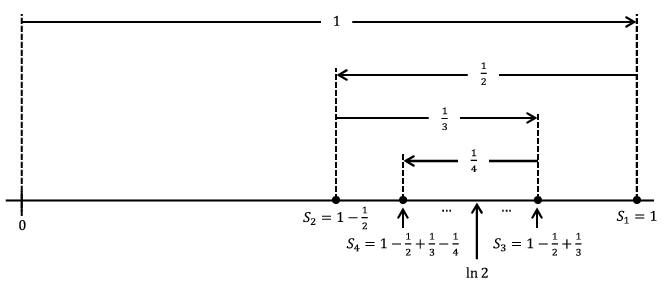
\includegraphics[width=\linewidth]{external/images/AltHarmonic.png}
\end{image}%
From the diagram we can see \(S_2\leq S_4\leq S_6\leq\cdots\leq\cdots\leq S_5\leq S_3\leq S_1\) and \(S_{2k+1}-S_{2k}=\frac{1}{2k+1}\). It seems that the sequence of partial sums will converge to whatever is in the ``middle.'' Our diagram indicates that it is ln \(2\) in the middle but actually this is not obvious. Nonetheless it is interesting that one series converges for \(x=1\) but the other does not.%
\begin{problem}{Problem}{}{PowerSeriesQuestions-SeriesAnomalies-11}%
\index{series!Taylor's series!used to approximate \(\ln 2\)} Use the fact that%
\begin{equation*}
1-\frac{1}{2}+\frac{1}{3}-\cdots+\frac{(-1)^{2k+1}}{2k}\leq\ln 2\leq 1-\frac{1}{2}+\frac{1}{3}-\cdots+\frac{(-1)^{2k+2}}{2k+1}
\end{equation*}
to determine how many terms of the series \(\sum_{n=1}^\infty\frac{(-1)^{n+1}}{n}\) should be added together to approximate \(\ln 2\) to within \(.0001\) without actually computing what \(\ln 2\) is.%
\end{problem}
These examples illustrate something even more perplexing.  As we've observed the divergent infinite sum \(1-1+1-1+\cdots\) does not appear satisfy the associative law for addition. Since the sum diverges (is meaningless) this is not too surprising.  On the other hand while the convergent series \(1-\frac{1}{2}+\frac{1}{3}-\cdots\) does satisfy the associative law as expected, it does not satisfy the commutative law.  In fact, \hyperref[thm_rearrangements]{Theorem~{\xreffont\ref{thm_rearrangements}}} shows that it fails,  rather spectacularly, to be commutative.%
\par
\index{Riemann, Bernhard} \href{https://mathshistory.st-andrews.ac.uk/Biographies/Riemann/}{Bernhard Riemann} (1826\textendash{}1866) stated and proved a generalization of the following theorem in 1854.%
\begin{figureptx}{Figure}{Bernhard Riemann}{FIGURERiemann}{}%
\index{Portraits!Riemann}%
\index{Riemann, Bernhard!portrait of}%
\begin{image}{0.325}{0.35}{0.325}{}%
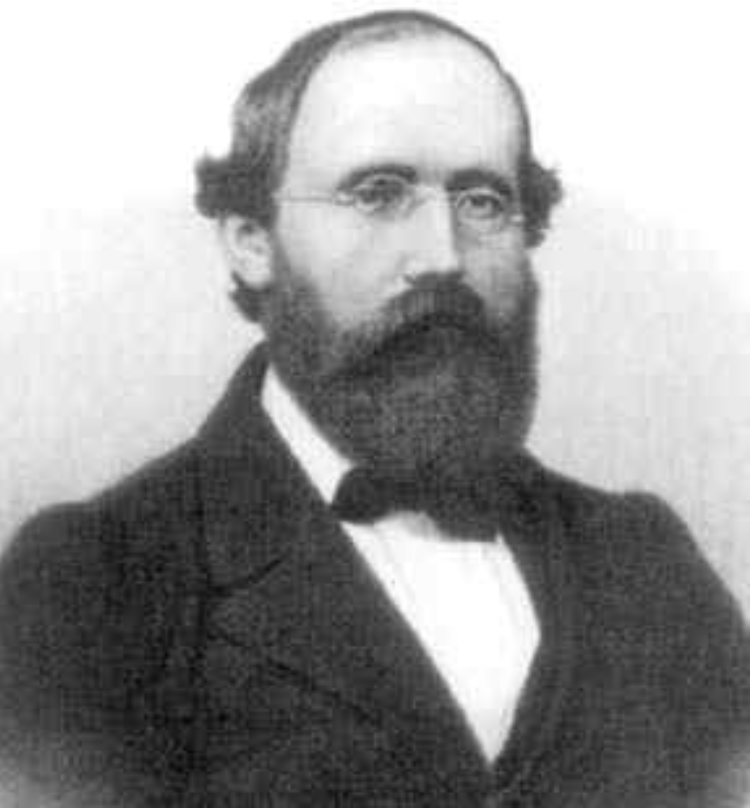
\includegraphics[width=\linewidth]{external/images/Riemann.png}
\end{image}%
\tcblower
\end{figureptx}%
\begin{theorem}{Theorem}{}{}{thm_rearrangements}%
\index{series!Alternating Harmonic Series!rearrangements of}%
Let \(a\) be any real number.  There exists a \terminology{rearrangement} of the \terminology{Alternating Harmonic Series} \(1-\frac{1}{2}+\frac{1}{3}-\cdots\) which converges to \(a\).%
\end{theorem}
\begin{aside}{Aside}{Series Rearrangements.}{PowerSeriesQuestions-SeriesAnomalies-16}%
A \terminology{rearrangement} of a series is another series which contains all of the terms of the original but not necessarily in the same order. For example one \terminology{rearrangment} of the \terminology{Alternating Harmonic Series}:%
\begin{equation*}
1-\frac{1}{2}+\frac{1}{3}-\frac{1}{4}+\frac{1}{5}-\frac{1}{6}\cdots{}
\end{equation*}
is%
\begin{equation*}
-\frac{1}{2}+1-\frac{1}{4}+\frac{1}{3}-\frac{1}{6}+\frac{1}{5}-\cdots{}\text{.}
\end{equation*}
%
\end{aside}
This theorem shows that a series is most decidedly not a great big sum.  It follows that power series are not just great big polynomials.%
\par
\index{series!Harmonic Series} To set the stage, consider the \terminology{Harmonic Series}%
\begin{equation}
\sum_{n=1}^\infty\frac{1}{n}=1+\frac{1}{2}+\frac{1}{3}+\cdots\text{.}\label{EQUATIONHarmonicSeries}
\end{equation}
%
\par
Even though the individual terms in this series converge to \(0\), the series still diverges (to infinity) as evidenced by the inequality%
\begin{align*}
\left(1+\frac{1}{2}\right)\amp +\left(\frac{1}{3}+\frac{1}{4}\right)+\left(\frac{1}{5}+\frac{1}{6}+ \frac{1}{7}+\frac{1}{8}\right)+\left(\frac{1}{9}+\cdots+\frac{1}{16}\right)+\cdots\\
\amp >\frac{1}{2}+\left(\frac{1}{4}+\frac{1}{4}\right)+\left(\frac{1}{8}+ \frac{1}{8}+\frac{1}{8}+\frac{1}{8}\right)+\left(\frac{1}{16}+\cdots+\frac{1}{16}\right)+\cdots\\
\amp =\frac{1}{2}+\frac{1}{2}+\frac{1}{2}+\frac{1}{2}+\cdots\\
\amp =   \infty\text{.}
\end{align*}
%
\par
Armed with this fact, we can see why \hyperref[thm_rearrangements]{Theorem~{\xreffont\ref{thm_rearrangements}}} is true. First note that%
\begin{equation*}
-\frac{1}{2}-\frac{1}{4}-\frac{1}{6}-\cdots=-\frac{1}{2}(1+\frac{1}{2}+ \frac{1}{3}+\cdots)=-\infty
\end{equation*}
and%
\begin{equation*}
1+\frac{1}{3}+\frac{1}{5}+\cdots\geq\frac{1}{2}+\frac{1}{4}+\frac{1}{6}+\ldots= \infty\text{.}
\end{equation*}
%
\par
This says that if we add enough terms of \(-\frac{1}{2}-\frac{1}{4}-\frac{1}{6}-\cdots\) we can make such a sum as large as we wish (and negative) and if we add enough terms of \(1+\frac{1}{3}+\frac{1}{5}+\cdots\) we can make such a sum as large as we wish (and positive).  Those facts provide us with the general outline of the proof.  The trick is to add just enough positive terms until the sum is just greater than \(a\).  Then we start to add on negative terms until the sum is just less than \(a\).  Picking up where we left off with the positive terms, we add on just enough positive terms until we are just above \(a\) again.  We then add on negative terms until we are below \(a\).  In essence, we are bouncing back and forth around \(a\).  If we do this carefully, then we can get this rearrangement to converge to \(a\).  The notation in the proof below gets a bit hairy, but keep this general idea in mind as you read through it.%
\par
Let \(O_1\) be the first odd integer such that \(1+\frac{1}{3}+\frac{1}{5}+\cdots+\frac{1}{O_1}>a\). Now choose \(E_1\) to be the first even integer such that%
\begin{equation*}
-\frac{1}{2}-\frac{1}{4}-\frac{1}{6}-\cdots-\frac{1}{E_1} \lt a-\left(1+\frac{1}{3}+\frac{1}{5}+\cdots+\frac{1}{O_1}\right)\text{.}
\end{equation*}
%
\par
Thus%
\begin{equation*}
1+\frac{1}{3}+\frac{1}{5}+\cdots+\frac{1}{O_1}-\frac{1}{2}-\frac{1}{4} - \frac{1}{6}-\cdots-\frac{1}{E_1}\lt a\text{.}
\end{equation*}
%
\par
Notice that we still have \(\frac{1}{O_1+2}+\frac{1}{O_1+4}+\cdots=\infty\). With this in mind, choose \(O_2\) to be the first odd integer with%
\begin{align*}
\frac{1}{O_1+2}\amp{}+\frac{1}{O_1+4}+\cdots\frac{1}{O_2}\\
\amp{}\gt          a-\left(1+\frac{1}{3}+
\frac{1}{5}+\cdots+\frac{1}{O_1}-\frac{1}{2}-\frac{1}{4}-\frac{1}{6}-\cdots-
\frac{1}{E_1}\right).
\end{align*}
%
\par
Thus we have%
\begin{align*}
a\lt
1+\frac{1}{3}+\frac{1}{5}+\amp{}\cdots+\frac{1}{O_1}-\frac{1}{2}-\frac{1}{4}-
\frac{1}{6}-\\
\amp{}\cdots-\frac{1}{E_1}+\frac{1}{O_1+2}+\frac{1}{O_1+4}+\cdots+
\frac{1}{O_2}.
\end{align*}
%
\par
Furthermore, since%
\begin{align*}
a\gt 1+\frac{1}{3}+\frac{1}{5}+\amp{}\cdots+\frac{1}{O_1}-\frac{1}{2}-\frac{1}{4}-
\frac{1}{6}-\\
\amp{}\cdots-\frac{1}{E_1}+\frac{1}{O_1+2}+\frac{1}{O_1+4}+\\
\amp{}\cdots+ \frac{1}{O_2-2}
\end{align*}
we have%
\begin{align*}
\frac{1}{O_2} \gt \left|1+\frac{1}{3}+\frac{1}{5}+\right.\amp{}\cdots+\frac{1}{O_1}-\frac{1}{2}-\frac{1}{4}- \frac{1}{6}-\\
\amp\cdots \left.-\frac{1}{E_1}+\frac{1}{O_1+2}+\frac{1}{O_1+4}+\cdots+ \frac{1}{O_2}-a\right|
\end{align*}
%
\par
In a similar fashion choose \(E_2\) to be the first even integer such that%
\begin{align*}
a\gt 1+\frac{1}{3}+\frac{1}{5}+\cdots\amp +\frac{1}{O_1}-\frac{1}{2}- \frac{1}{4}-\frac{1}{6}-\\
\cdots\amp{} -\frac{1}{E_1}+ \frac{1}{O_1+2}+\frac{1}{O_1+4}+\\
\cdots\amp{}+\frac{1}{O_2}-\frac{1}{E_1+2}-\frac{1}{E_1+4}- \cdots{}-\frac{1}{E_2}\text{.}
\end{align*}
%
\par
Since%
\begin{align*}
a\lt 1+\frac{1}{3}+\frac{1}{5} +\cdots\amp{}+\frac{1}{O_1}-\frac{1}{2}- \frac{1}{4}-\frac{1}{6}-\\
\cdots\amp{}-\frac{1}{E_1}+ \frac{1}{O_1+2}+\frac{1}{O_1+4}+\\
\cdots\amp{}+\frac{1}{O_2}- \frac{1}{E_1+2}-\frac{1}{E_1+4}-\cdots-\frac{1}{E_2-2}
\end{align*}
we see that%
\begin{align*}
\frac{1}{E_2} \gt{}
\left|1+\frac{1}{3}\right.+\frac{1}{5}+
\amp \cdots+\frac{1}{O_1}-\frac{1}{2}-
\frac{1}{4}-\frac{1}{6}-\\
\amp{}\cdots-\frac{1}{E_1} +\frac{1}{O_1+2}+\frac{1}{O_1+4}+\\
\amp{}\cdots+\frac{1}{O_2}-
\frac{1}{E_1+2}-\frac{1}{E_1+4}-\\
\amp{}\cdots-\left.\frac{1}{E_2}-a\right|.
\end{align*}
%
\par
Again choose \(O_3\) to be the first odd integer such that%
\begin{align*}
a\lt 1+\frac{1}{3} +\frac{1}{5}+
\amp{}\cdots+\frac{1}{O_1}-\frac{1}{2}-\frac{1}{4}- \frac{1}{6}-\\
\amp{}\cdots
-\frac{1}{E_1}+\frac{1}{O_1+2}+\frac{1}{O_1+4}+\\
\amp{}\cdots+\frac{1}{E_1+2}-\frac{1}{E_1+4}-\cdots -\frac{1}{E_2} +\\
\amp{} \cdots \frac{1}{O_2+2} + \frac{1}{O_2+4}\cdots+\frac{1}{O_3}
\end{align*}
and notice that%
\begin{align*}
\frac{1}{O_3}\gt          \left|1+\frac{1}{3}\right.
+\frac{1}{5}+\amp{}\cdots+\frac{1}{O_1}-\frac{1}{2}-\frac{1}{4}-\frac{1}{6}-\\
\amp
\cdots-\frac{1}{E_1}+\frac{1}{O_1+2}+\frac{1}{O_1+4}+\\
\amp \cdots+ \frac{1}{O_2}+
-\frac{1}{E_1+2}-\frac{1}{E_1+4}-\\
\amp{}\cdots-\frac{1}{E_2}+\frac{1}{O_2+2}+
\frac{1}{O_2+4}+\cdots+\left.\frac{1}{O_3}-a\right|\text{.}
\end{align*}
%
\par
Continue defining \(O_k\) and \(E_k\) in this fashion for \(k\ge 4\). Since \(\limit{k}{\infty}{\frac{1}{O_k}}=\limit{k}{\infty}{\frac{1}{E_k}}=0\), it is evident that the partial sums%
\begin{align*}
1+\frac{1}{3} +\frac{1}{5}+\amp{}\cdots+\frac{1}{O_1}-\frac{1}{2}-\frac{1}{4}-\frac{1}{6}-\\
\amp \cdots-\frac{1}{E_1}+\frac{1}{O_1+2}+\frac{1}{O_1+4}+\\
\amp \cdots \frac{1}{O_2}+\cdots -\frac{1}{E_{k-2}+2}-\frac{1}{E_{k-2}+4}-\\
\amp \cdots-\frac{1}{E_{k-1}}+  \frac{1}{O_{k-1}+2}+\frac{1}{O_{k-1}+4}+\cdots+\frac{1}{O_k}
\end{align*}
and%
\begin{align*}
1+\frac{1}{3}\amp
+\frac{1}{5}+\cdots+\frac{1}{O_1}-\frac{1}{2}-\frac{1}{4}-
\frac{1}{6}-\\
\amp \cdots-\frac{1}{E_1}+\frac{1}{O_1+2}+\frac{1}{O_1+4}+
\cdots{} \frac{1}{O_2}+\\
\amp
\cdots-\frac{1}{E_{k-2}+2}-\frac{1}{E_{k-2}+4}-\cdots-\frac{1}{E_{k-1}}
\end{align*}
must converge to \(a\). Furthermore, it is evident that every partial sum of the rearrangement%
\begin{align*}
1+\frac{1}{3} +\frac{1}{5}+\amp\cdots+\frac{1}{O_1}-\frac{1}{2}-\frac{1}{4}- \frac{1}{6}-\\
\amp{}-\cdots-\frac{1}{E_1}+\frac{1}{O_1+2}+\frac{1}{O_1+4}+\cdots+ \frac{1}{O_2}+\cdots
\end{align*}
is trapped between two such extreme partial sums. This forces the entire rearranged series to converge to \(a\).%
\par
The two parts of the \hyperref[DRILLprob_RearrangeDivToInf]{next problem} are extentions of \hyperref[thm_rearrangements]{Theorem~{\xreffont\ref{thm_rearrangements}}} but they are a bit simpler notationally since we don't need to worry about converging to an actual number.  We only need to make the rearrangement increase or decrease without bound.%
\begin{problem}{Problem}{}{DRILLprob_RearrangeDivToInf}%
Show that there is a rearrangement of the \terminology{Alternating Harmonic Series},%
\begin{equation*}
1-\frac{1}{2}+\frac{1}{3}-\frac{1}{4}+\cdots
\end{equation*}
which:%
\begin{enumerate}[font=\bfseries,label=(\alph*),ref=\alph*]%
\item{}Diverges to \(\infty\).%
\item{}Diverges to \(-\infty\).%
\end{enumerate}%
\end{problem}
It is fun to know that we can rearrange some series to make them add up to anything we like but there is a more fundamental idea at play here.  That the negative terms of the Alternating Harmonic Series diverge to negative infinity and the positive terms diverge to positive infinity make the convergence of the alternating series very special.%
\par
Consider what happens when we sum the series.  We start with \(1\). This is a positive term so our sum is starting to increase without bound.  Next we add \(-1/2\) which is a negative terms so our sum has turned around and is now starting to decrease without bound.  Then another positive term is added: increasing without bound.  Then another negative term: decreasing.  And so on.  The convergence of the alternating Harmonic Series is the result of a delicate balance between a tendency to run off to positive infinity and back to negative infinity.  When viewed in this light it is not really too surprising that rearranging the terms can destroy this delicate balance.%
\par
Naturally, the alternating Harmonic Series is not the only such series. Any such series is said to \terminology{converge conditionally} \textemdash{} the condition being the specific arrangement of the terms.%
\par
To stir the pot a bit more, some series do satisfy the commutative property.  More specifically, one can show that any rearrangement of the series \(1-\frac{1}{2^2}+\frac{1}{3^2}-\cdots\) must converge to the same value as the original series (which happens to be \(\int_{x=0}^1\frac{\ln(1+x)}{x}\dx{x}\approx.8224670334\)).  Why does one series behave so nicely whereas the other does not?%
\par
Anomalies like these were well known in the \(1700\)s, but they were overshadowed by the overwhelming utility of the Calculus.  Indeed, foundational questions raised by the above examples as well as concerns about the validity of using the infinitely small and infinitely large, while certainly interesting and of importance, did not significantly deter the exploitation of Calculus in studying physical phenomena. However, the envelope eventually was pushed to the point that not even the most practically oriented mathematician could avoid these foundational issues.%
\end{sectionptx}
\end{chapterptx}
\end{partptx}
%
%
\typeout{************************************************}
\typeout{Part II Interregnum}
\typeout{************************************************}
%
\begin{partptx}{Part}{Interregnum}{}{Interregnum}{}{}{InterregnumPart}
\renewcommand*{\partname}{Part}
%
%
\typeout{************************************************}
\typeout{Chapter 5 Joseph Fourier: The Man Who Broke Calculus}
\typeout{************************************************}
%
\begin{chapterptx}{Chapter}{Joseph Fourier: The Man Who Broke Calculus}{}{Joseph Fourier: The Man Who Broke Calculus}{}{}{Interegnum}
\renewcommand*{\chaptername}{Chapter}
%
%
\typeout{************************************************}
\typeout{Section 5.1 Joseph Fourier and His Series}
\typeout{************************************************}
%
\begin{sectionptx}{Section}{Joseph Fourier and His Series}{}{Joseph Fourier and His Series}{}{}{Interegnum-2}
Applying mathematics to physical problems such as heat flow in a solid body drew much attention in the latter part of the 1700's and the early part of the 1800's.  One of the people to attack the heat flow problem was \href{https://mathshistory.st-andrews.ac.uk/Biographies/Fourier/}{Jean Baptiste Joseph Fourier} (1768\textendash{}1839).%
\begin{figureptx}{Figure}{Jean Baptiste Joseph Fourier}{Interegnum-2-3}{}%
\index{Fourier, Jean Baptiste Joseph!portrait of}%
\index{Portraits!Fourier}%
\begin{image}{0.325}{0.35}{0.325}{}%
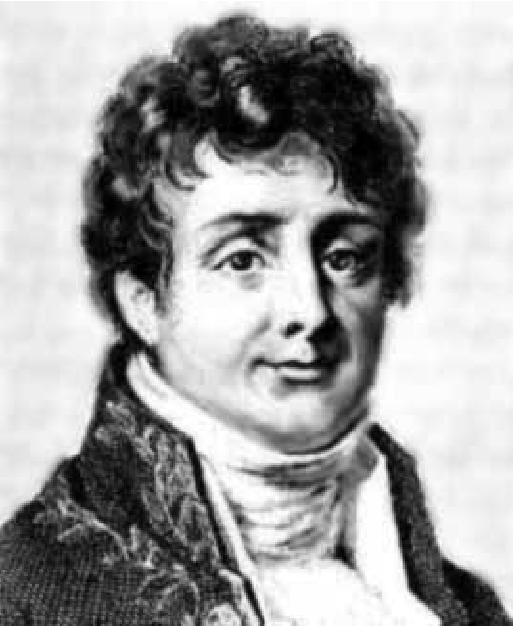
\includegraphics[width=\linewidth]{external/images/Fourier.png}
\end{image}%
\tcblower
\end{figureptx}%
\index{Fourier, Jean Baptiste Joseph} Fourier submitted a manuscript on the subject, \textit{Sur la propagation de la chaleur} (\pubtitle{On the Propagation of Heat}), to the \textit{Institut National des Sciences et des Arts} in 1807.  These ideas were subsequently published in \textit{La theorie analytique de la chaleur} (\pubtitle{The Analytic Theory of Heat (1822)}).%
\par
To examine Fourier's ideas, consider the example of a thin wire of length one, which is perfectly insulated and whose endpoints are held at a fixed temperature of zero.  Given an initial temperature distribution in the wire, the problem is to monitor the temperature of the wire at any point \(x\) and at any time \(t\).  Specifically, if we let \(u(x,t)\) denote the temperature of the wire at point \(x\in[0,1]\) at time \(t\geq 0\), then it can be shown that \(u\) must satisfy the one-dimensional heat equation \(\rho^2\frac{\partial^2u}{\partial x^2}=\frac{\partial
u}{\partial t}\), where \(\rho^2\) is a positive constant known as the \terminology{thermal diffusivity}.  If the initial temperature distribution is given by the function \(f(x)\), then the \(u\) we are seeking must satisfy all of the following%
\begin{align}
\rho^2\frac{\partial^2u}{\partial x^2}\amp{}=\frac{\partial u}{\partial t},\amp{}\label{EQUATIONHeatEquation}\\
u(0,t)\amp{} =u(1,t)=0,  
\amp{}
\forall t\amp{}\geq 0,\notag\\
u(x,0)\amp{} =f(x), 
\amp{}
\forall x\amp{}\in[\,0,1].\notag
\end{align}
%
\par
To do this, Fourier employed what is now referred to as the method of separation of variables.  Specifically, Fourier looked for solutions of the form \(u(x,t)=X(x)T(t)\); that is, solutions where the \(x\)-part can be separated from the \(t\)-part.  Assuming that \(u\) has this form, we get \(\frac{\partial^2u}{\partial x^2}=X^{\prime\prime}T\) and \(\frac{\partial u}{\partial t}=X\,T^{\prime}\).  Substituting these into \hyperref[EQUATIONHeatEquation]{equation~({\xreffont\ref{EQUATIONHeatEquation}})} \(\rho^2\frac{\partial^2u}{\partial x^2}=\frac{\partial
u}{\partial t}\), we obtain%
\begin{align*}
\rho^2X^{\prime\prime}T=X
T^\prime\amp{}\amp{}\text{or}\amp{}\amp{}
\frac{X^{\prime\prime}}{X}=\frac{T^\prime}{\rho^2T}\text{.}
\end{align*}
%
\par
Since the left-hand side involves no \(t\)'s and the right-hand side involves no \(x\)'s, both sides must equal a constant \(k\). Thus we have%
\begin{align*}
X^{\prime\prime}=k X\amp{}\amp{}\text{and}\amp{}\amp{}
T^\prime=\rho^2k T.
\end{align*}
%
\begin{problem}{Problem}{}{prob_HarmonicMotion}%
Show that \(T=Ce^{\rho^2kt}\) satisfies the equation \(T^\prime=\rho^2k T\), where \(C\) is an arbitrary constant.  Use the physics of the problem to show that if \(u\) is not constantly zero, then \(k\lt 0\).%
\par\smallskip%
\noindent\textbf{\blocktitlefont Hint}.\hypertarget{prob_HarmonicMotion-4}{}\quad{}Consider \(\limit{t}{\infty}{u(x,t)}\).%
\end{problem}
Using the result from \hyperref[prob_HarmonicMotion]{Problem~{\xreffont\ref{prob_HarmonicMotion}}} that \(k\lt 0\), we will let \(k=-p^2\).%
\begin{problem}{Problem}{}{Interegnum-2-10}%
Show that \(X=A\sin\left(px\right)+B\cos\left(px\right)\) satisfies the equation \(X^{\prime\prime}=-p^2X\), where \(A\) and \(B\) are arbitrary constants.  Use the boundary conditions \(u(0,t)=u(1,t)=0\), \(\forall\) \(t\geq 0\) to show that \(B=0\) and \(A\sin p=0\).  Conclude that if \(u\) is not constantly zero, then \(p=n\pi\), where \(n\) is any integer.%
\end{problem}
\begin{problem}{Problem}{}{Interegnum-2-11}%
Show that if \(u_1\) and \(u_2\) satisfy the equations%
\begin{equation*}
\rho^2\frac{\partial^2u}{\partial x^2}=\frac{\partial
u}{\partial t}
\end{equation*}
and%
\begin{align*}
u(0,t)=u(1,t)=0,\amp{}\amp{} \forall\  t\geq   0
\end{align*}
then \(u=A_1u_1+A_2u_2\) satisfy them as well, where \(A_1\) and \(A_2\) are arbitrary constants.%
\end{problem}
\index{Fourier, Jean Baptiste Joseph} Putting all of these results together, Fourier surmised that the general solution to%
\begin{align*}
\rho^2\frac{\partial^2u}{\partial x^2}=\frac{\partial
u}{\partial t} u(0,t)=u(1,t)=0,\amp{}\amp{}\forall\ t\geq 0
\end{align*}
could be expressed as the series%
\begin{equation*}
u(x,t)=\sum_{n=1}^\infty A_ne^{-(\rho n\pi)^2t}\sin\left(n\pi x\right)\text{.}
\end{equation*}
%
\par
All that is left is to have \(u\) satisfy the initial condition \(u(x,0)=f(x)\), \(\forall\,x\in[\,0,1]\). That is, we need to find coefficients \(A_n\), such that%
\begin{equation*}
f(x)=u(x,0)=\sum_{n=1}^\infty A_n\sin\left(n\pi x\right)\text{.}
\end{equation*}
%
\par
The idea of representing a function as a series of sine waves was proposed by Daniel Bernoulli in 1753 while examining the problem of modeling a vibrating string. Unfortunately for Bernoulli, he didn't know how to compute the coefficients in such a series representation. What distinguished Fourier was that he developed a technique to compute these coefficients. The key is the result of the following problem.%
\begin{problem}{Problem}{}{prob_SinOrthogonality}%
Let \(n\) and \(m\) be positive integers. Show%
\begin{equation*}
\int_{x=0}^1\sin\left(n\pi x\right)\sin\left(m\pi x\right)\dx{ x}= \left\{\begin{matrix}0\amp \text{ if } n\neq m\\ \frac{1}{2}\amp \text{ if } n=m \end{matrix} \right.. {}
\end{equation*}
%
\end{problem}
\index{Fourier, Jean Baptiste Joseph} Armed with the result from \hyperref[prob_SinOrthogonality]{Problem~{\xreffont\ref{prob_SinOrthogonality}}}, Fourier could compute the coefficients \(A_n\) in the series representation \(f(x)=\sum_{n=1}^\infty A_n \sin\left(n\pi x\right)\) in the following manner.  Since we are trying to find \(A_n\) for a particular (albeit general) \(n\), we will temporarily change the index in the summation from \(n\) to \(j\).  With this in mind, consider%
\begin{align*}
\int_{x=0}^1f(x)\sin\left(n\pi x\right)\dx{ x} \amp =\int_{x=0}^1\left(\sum_{j=1}^\infty A_j\text{ sin } \left(j\pi x\right)\right)\sin\left(n\pi x\right)\dx{ x}\\
\amp =\sum_{j=1}^\infty A_j\int_{x=0}^1\sin\left(j\pi x\right)\sin\left(n\pi x\right)\dx{ x}\\
\amp =\frac{A_n}{2}
\end{align*}
which leads to the formula \(A_n=2\int_{x=0}^1f(x)\sin\left(n\pi x\right)d x\).%
\par
The series \(f(x)=\sum_{n=1}^\infty A_n\sin\left(n\pi
x\right)\) with%
\begin{equation}
A_n=2\int_{x=0}^1f(x)\sin\left(n\pi
x\right)\dx{ x}\label{EQUATIONSineCoeffFourier}
\end{equation}
is called the \emph{Fourier (sine) series of \(\boldsymbol{f}\)}.%
\begin{example}{Example}{}{Interegnum-2-18}%
Let's apply this to the function, \(f(x)=\frac{1}{2}-\abs{x-\frac{1}{2}}\), whose graph is seen below.%
\begin{image}{0.125}{0.75}{0.125}{}%
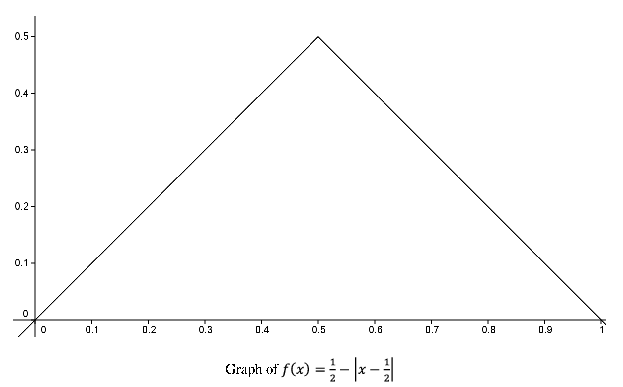
\includegraphics[width=\linewidth]{external/images/FourierEx1.png}
\end{image}%
\end{example}
\begin{problem}{Problem}{}{Interegnum-2-19}%
Let \(n\) be a positive integer. Show that if%
\begin{equation*}
f(x)=\frac{1}{2}-\abs{x-\frac{1}{2}}
\end{equation*}
then%
\begin{equation*}
\int_{x=0}^1f(x)\sin\left(n\pi x\right)d x = \frac{2}{\left(n\pi\right)^2}\sin\left(\frac{n\pi}{2}\right)
\end{equation*}
and show that the Fourier sine series of \(f\) is given by%
\begin{align*}
f(x)\amp{}=\sum_{n=1}^\infty\frac{4}{\left(n\pi\right)^2}\sin\left(\frac{n\pi}{2}
\right)\sin\left(n\pi x\right)\\
\amp{}=\frac{4}{\pi^2}\sum_{k=0}^\infty\frac{\left(-1\right)^k}{\left(2k+1\right)^2}\sin\left(\left(2k+1\right)\pi x\right).{}
\end{align*}
%
\end{problem}
To see evidence that this series really does, in fact, represent \(f\) on \([0,1]\), let%
\begin{equation*}
S_N(x)=\frac{4}{\pi^2}\sum_{k=0}^N\frac{\left(-1\right)^k}{\left(2k+1\right)^2} \sin\left(\left(2k+1\right)\pi x\right)
\end{equation*}
be the \(Nth\) partial sum of the series.     The sketches below display the graphs of \(S_N\) when \(N=1\), \(N=2\), \(N=5\), and \(N=50\).%
\begin{sidebyside}{2}{0.025}{0.025}{0.05}%
\begin{sbspanel}{0.45}[center]%
\begin{panelfigureptx}{Figure}{Graph of \(S_1(x)\)}{Interegnum-2-21-1-1}{}%
\noindent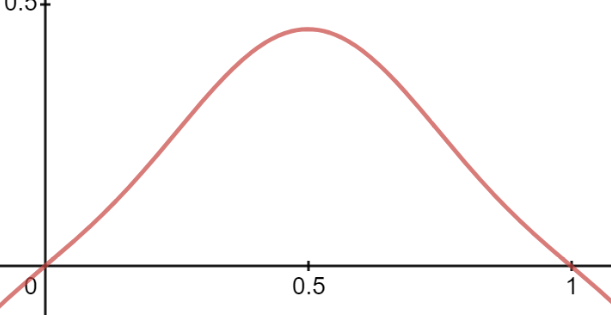
\includegraphics[width=\linewidth]{external/images/FourierEx2-1.png}
\tcblower
\end{panelfigureptx}%
\end{sbspanel}%
\begin{sbspanel}{0.45}[center]%
\begin{panelfigureptx}{Figure}{Graph of \(S_2(x)\)}{Interegnum-2-21-1-2}{}%
\noindent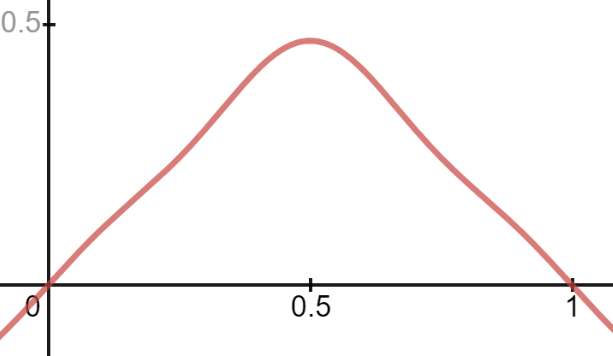
\includegraphics[width=\linewidth]{external/images/FourierEx3-1.png}
\tcblower
\end{panelfigureptx}%
\end{sbspanel}%
\end{sidebyside}%
\begin{sidebyside}{2}{0.025}{0.025}{0.05}%
\begin{sbspanel}{0.45}[center]%
\begin{panelfigureptx}{Figure}{Graph of \(S_5(x)\)}{Interegnum-2-21-2-1}{}%
\noindent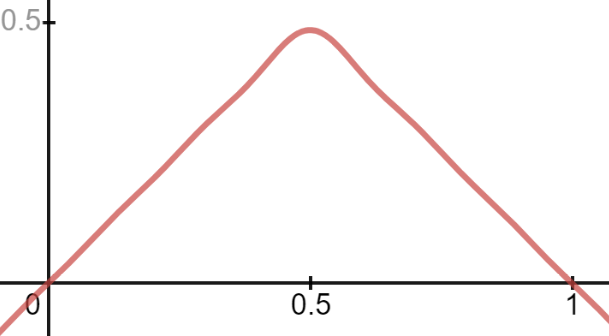
\includegraphics[width=\linewidth]{external/images/FourierEx4-1.png}
\tcblower
\end{panelfigureptx}%
\end{sbspanel}%
\begin{sbspanel}{0.45}[center]%
\begin{panelfigureptx}{Figure}{Graph of \(S_{50}(x)\)}{Interegnum-2-21-2-2}{}%
\noindent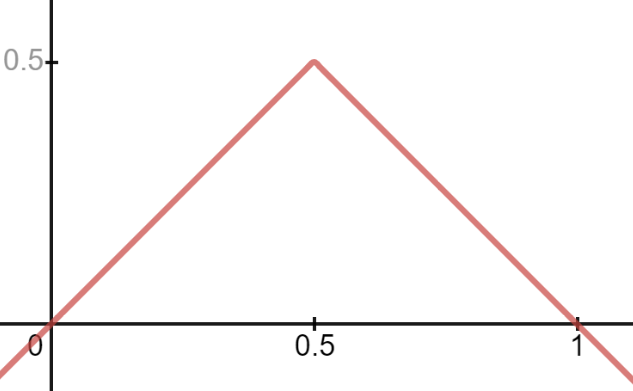
\includegraphics[width=\linewidth]{external/images/FourierEx5-1.png}
\tcblower
\end{panelfigureptx}%
\end{sbspanel}%
\end{sidebyside}%
As you can see, as we add more terms to \(S_N\) its graph looks more and more like the original function \(f(x)=\frac{1}{2}-\abs{x-\frac{1}{2}}\).  This would seem to be strong evidence that series converges to the function and therefore%
\begin{equation}
f(x)=\frac{4}{\pi^2}\sum_{k=0}^\infty\frac{\left(-1\right)^k}{\left(2k+1\right)^2}\sin\left(\left(2k+1\right)\pi x\right)\text{.}\label{PDE_sol}
\end{equation}
is a valid representation of \(f\) as a Fourier series.%
\par
But is it?%
\par
Recall, that when we represented a function as a power series, we freely differentiated and integrated the series term by term as though it was a polynomial. Let's do the same with this Fourier series.%
\par
To start, notice that the derivative of%
\begin{equation*}
f(x)=\frac{1}{2}-\abs{x-\frac{1}{2}}
\end{equation*}
is given by%
\begin{equation*}
f^\prime(x) = \begin{cases}1\amp \text{ if } \,\text{ } 0\leq x\lt \frac{1}{2}\\ -1\amp \text{ if } \,\frac{1}{2}\lt x\leq 1 \end{cases} \text{.}
\end{equation*}
%
\par
This derivative does not exist at \(x=\frac{1}{2}\) and its graph is given by%
\begin{figureptx}{Figure}{Graph of \(f^\prime(x) = 
\begin{cases}
1\amp \text{ if }  0\leq x\lt \frac{1}{2}\\ 
-1\amp \text{ if } \frac{1}{2}\lt x\leq 1 
\end{cases} \)}{Interegnum-2-27}{}%
\begin{image}{0.125}{0.75}{0.125}{}%
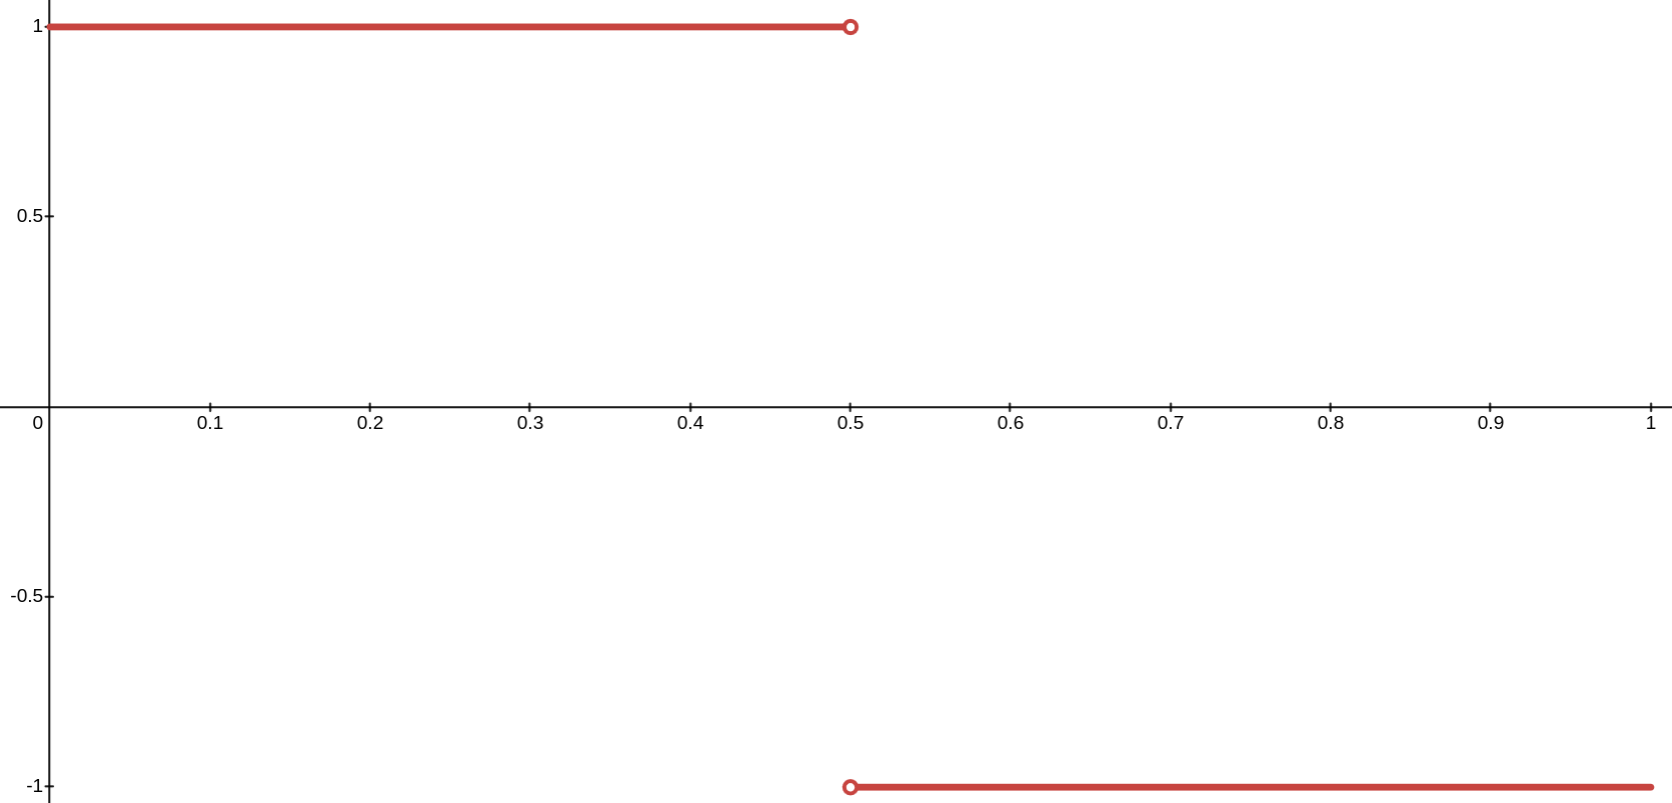
\includegraphics[width=\linewidth]{external/images/Ch2fig1-1.png}
\end{image}%
\tcblower
\end{figureptx}%
If we differentiate the Fourier series in \hyperref[PDE_sol]{equation~({\xreffont\ref{PDE_sol}})} term\textendash{}by\textendash{}term, we obtain%
\begin{equation}
\frac{4}{\pi}\sum_{k=0}^\infty\frac{\left(-1\right)^k}{\left(2k+1\right)}
\cos\left(\left(2k+1\right)\pi x\right) \text{.}\label{EQUATIONPDESolDeriv}
\end{equation}
Let \(C_N(x)=\frac{4}{\pi}\sum_{k=0}^N\frac{\left(-1\right)^k}{\left(2k+1\right)}
\cos\left(\left(2k+1\right)\pi x\right)\) be the \(Nth\) partial sum of this Fourier cosine series. The sketches below display the graphs of \(C_N\) when \(N=1\), \(N=2\), \(N=5\), and \(N=50\).%
\begin{sidebyside}{2}{0.025}{0.025}{0.05}%
\begin{sbspanel}{0.45}[center]%
\begin{panelfigureptx}{Figure}{Graph of \(C_1(x)\)}{Interegnum-2-29-1-1}{}%
\noindent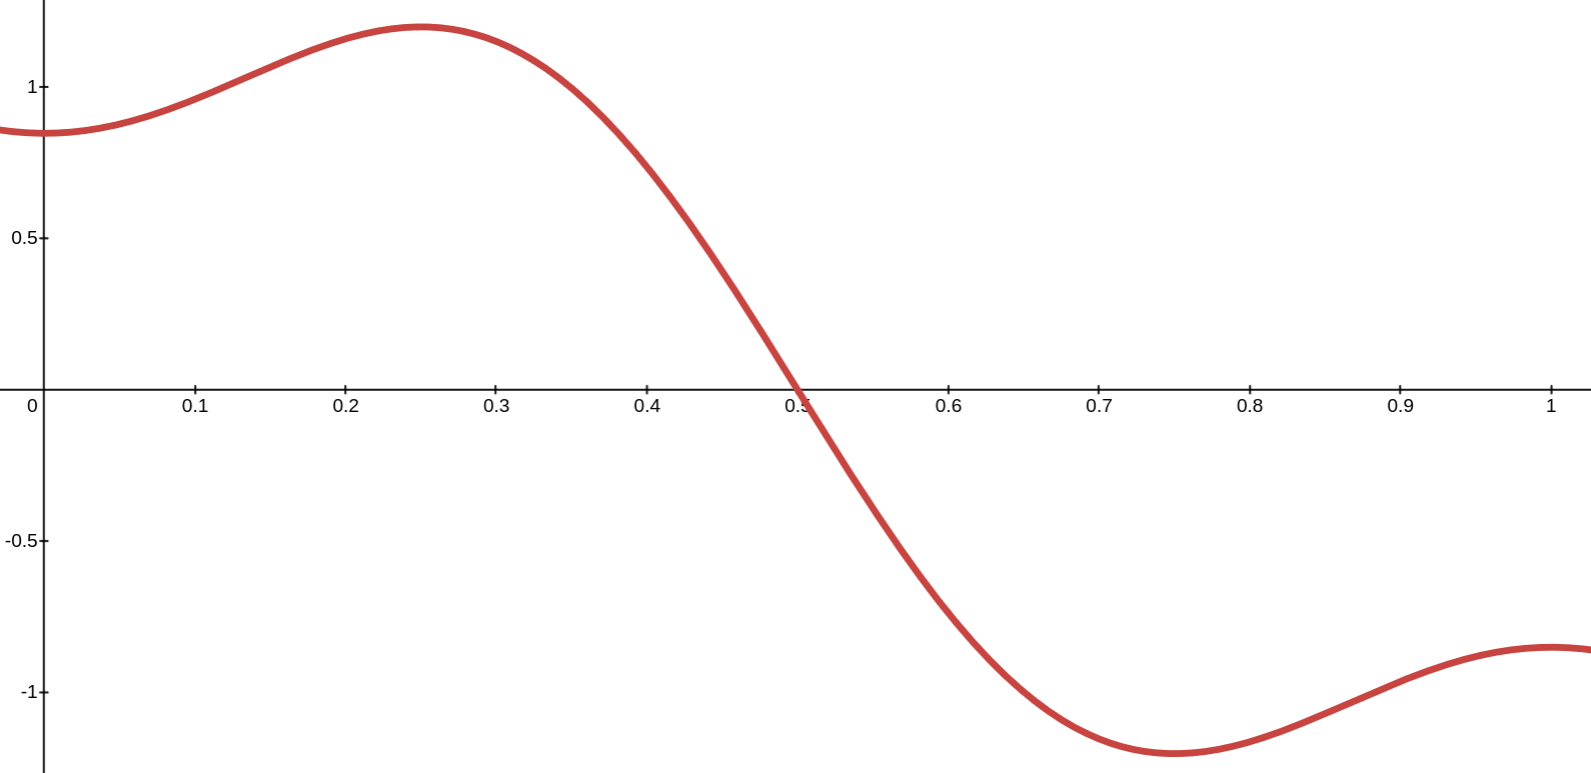
\includegraphics[width=\linewidth]{external/images/FourierEx6-1.png}
\tcblower
\end{panelfigureptx}%
\end{sbspanel}%
\begin{sbspanel}{0.45}[center]%
\begin{panelfigureptx}{Figure}{Graph of \(C_1(x)\)}{Interegnum-2-29-1-2}{}%
\noindent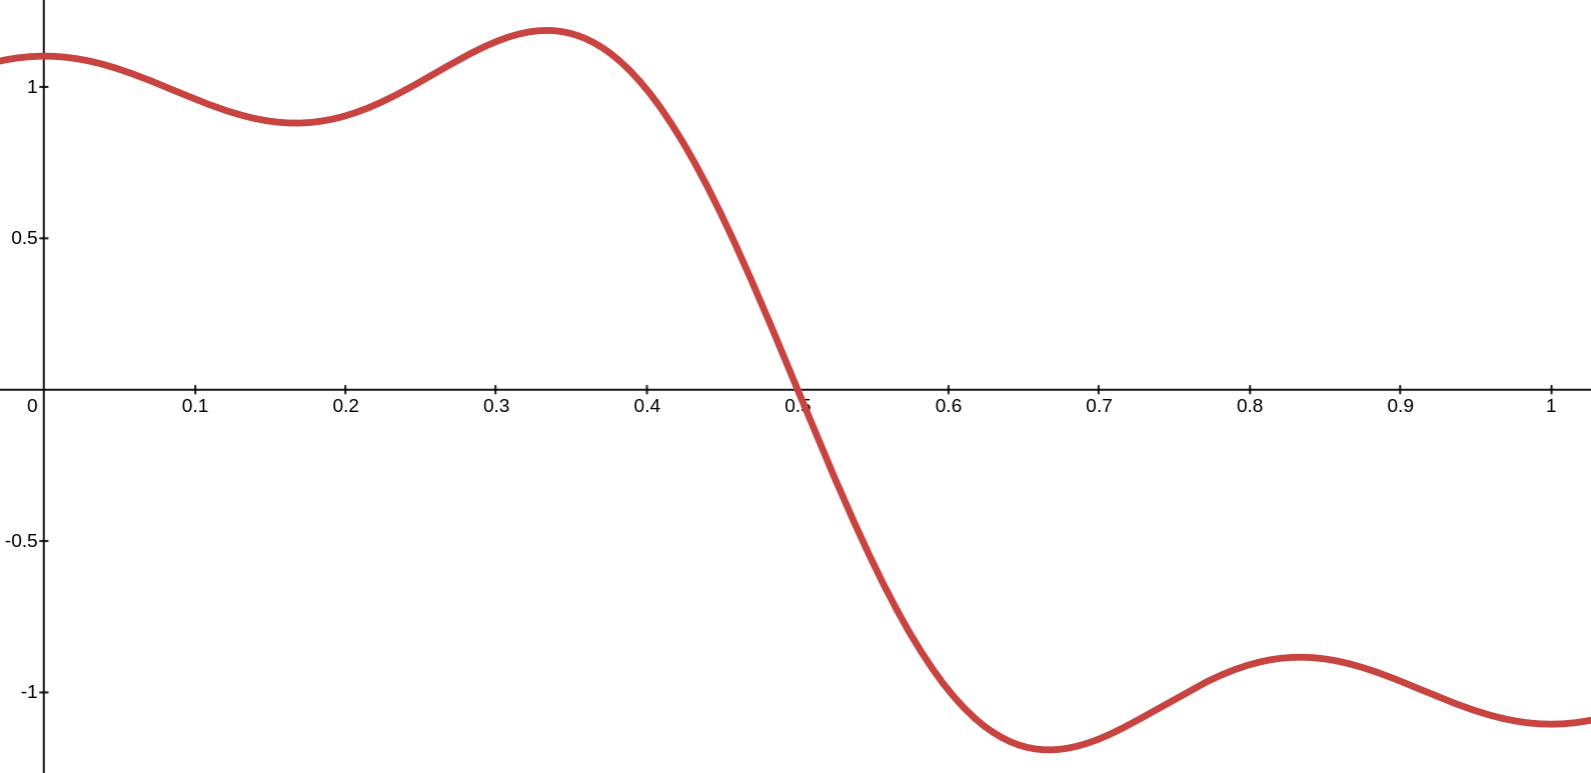
\includegraphics[width=\linewidth]{external/images/FourierEx7-1.png}
\tcblower
\end{panelfigureptx}%
\end{sbspanel}%
\end{sidebyside}%
\begin{sidebyside}{2}{0.025}{0.025}{0.05}%
\begin{sbspanel}{0.45}[center]%
\begin{panelfigureptx}{Figure}{Graph of \(C_5(x)\)}{Interegnum-2-29-2-1}{}%
\noindent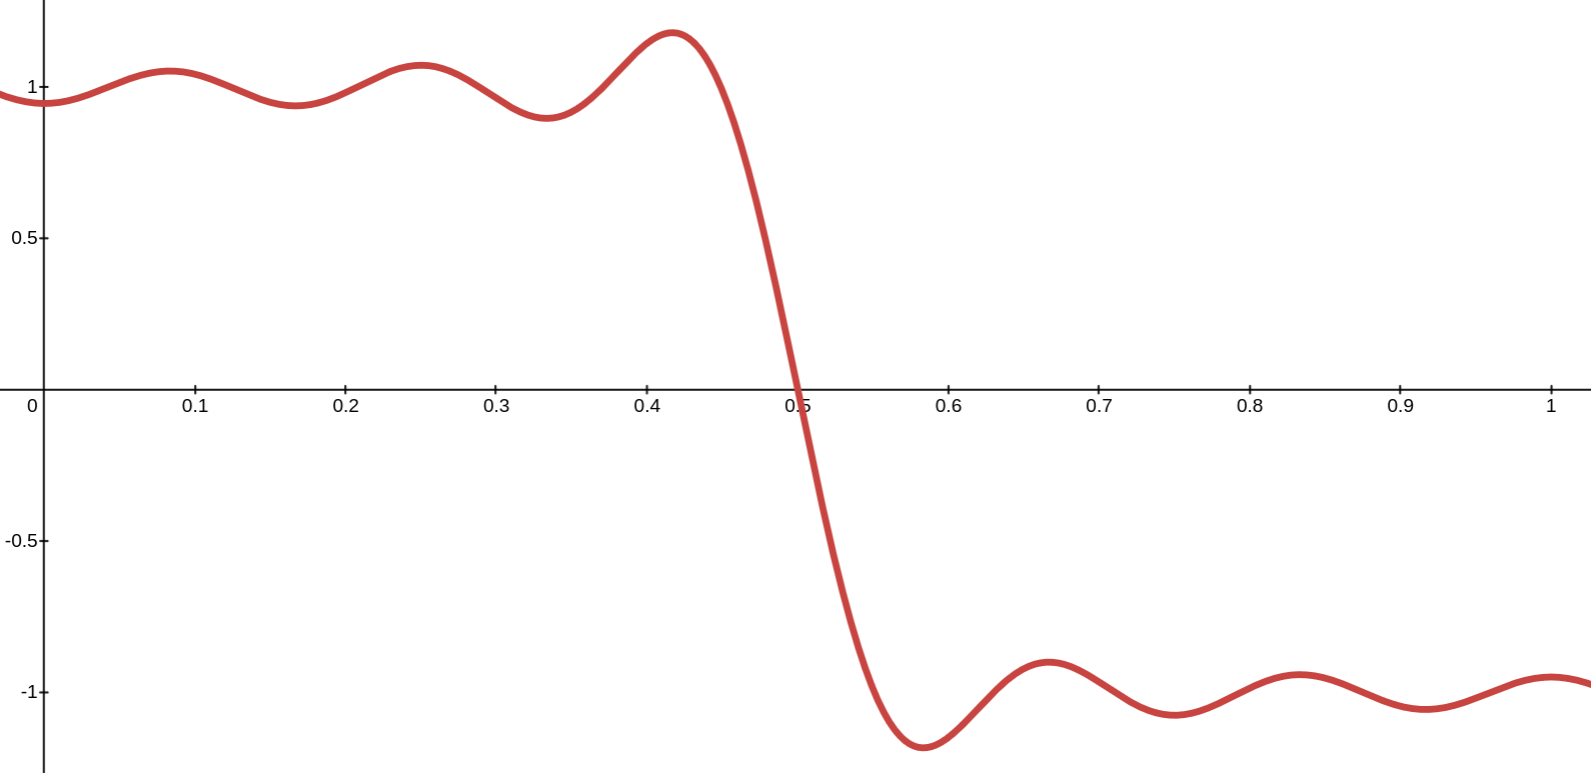
\includegraphics[width=\linewidth]{external/images/FourierEx8-1.png}
\tcblower
\end{panelfigureptx}%
\end{sbspanel}%
\begin{sbspanel}{0.45}[center]%
\begin{panelfigureptx}{Figure}{Graph of \(C_{50}(x)\)}{Interegnum-2-29-2-2}{}%
\noindent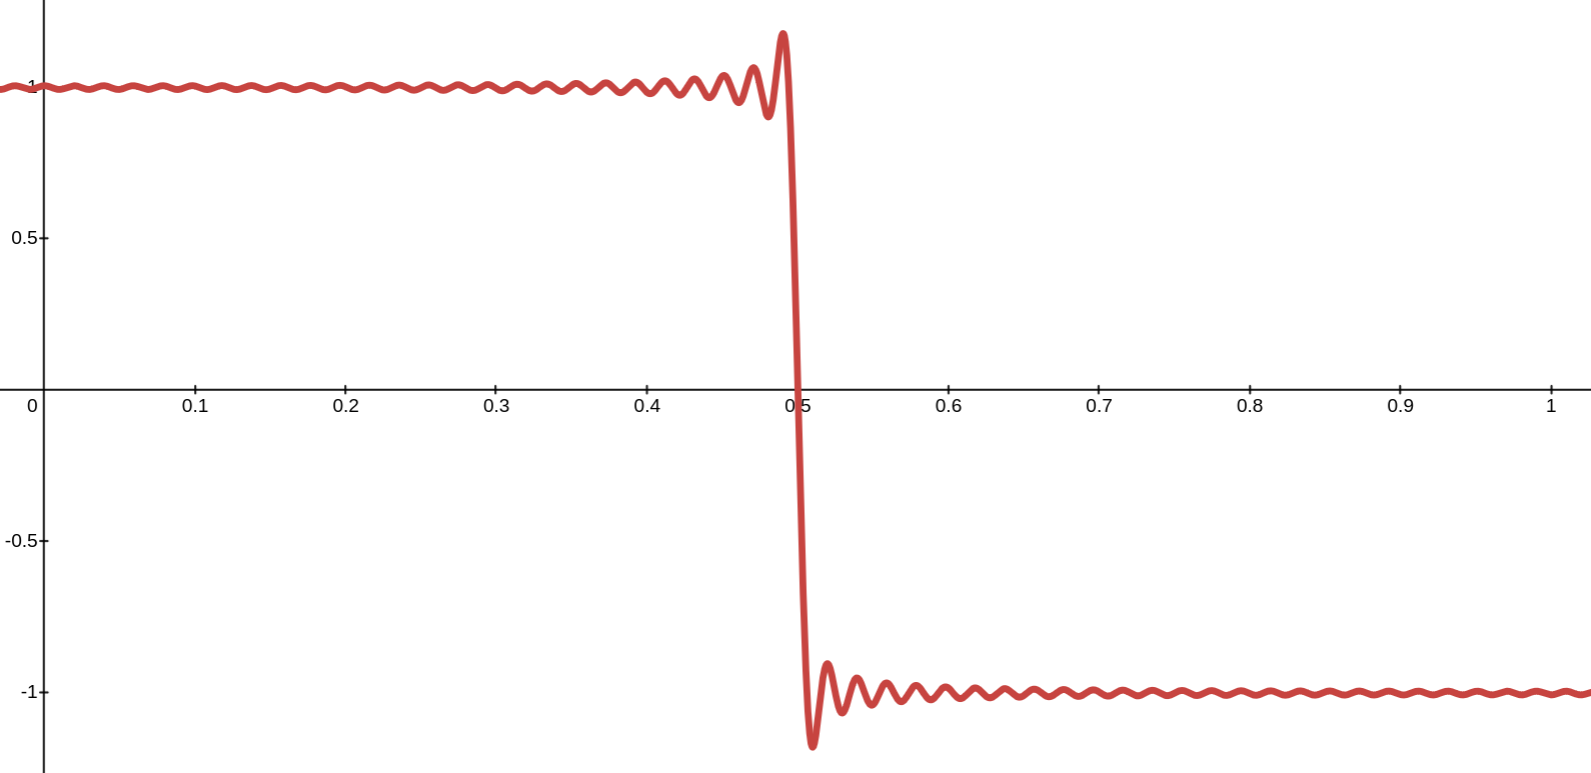
\includegraphics[width=\linewidth]{external/images/FourierEx9-1.png}
\tcblower
\end{panelfigureptx}%
\end{sbspanel}%
\end{sidebyside}%
In fact, if we were to graph the series \(\frac{4}{\pi}\sum_{k=0}^\infty\frac{\left(-1\right)^k}{\left(2k+1\right)}\) cos\(\left(\left(2k+1\right)\pi x\right)\), we would obtain the following graph:%
\begin{figureptx}{Figure}{}{Interegnum-2-31}{}%
\begin{image}{0.125}{0.75}{0.125}{}%
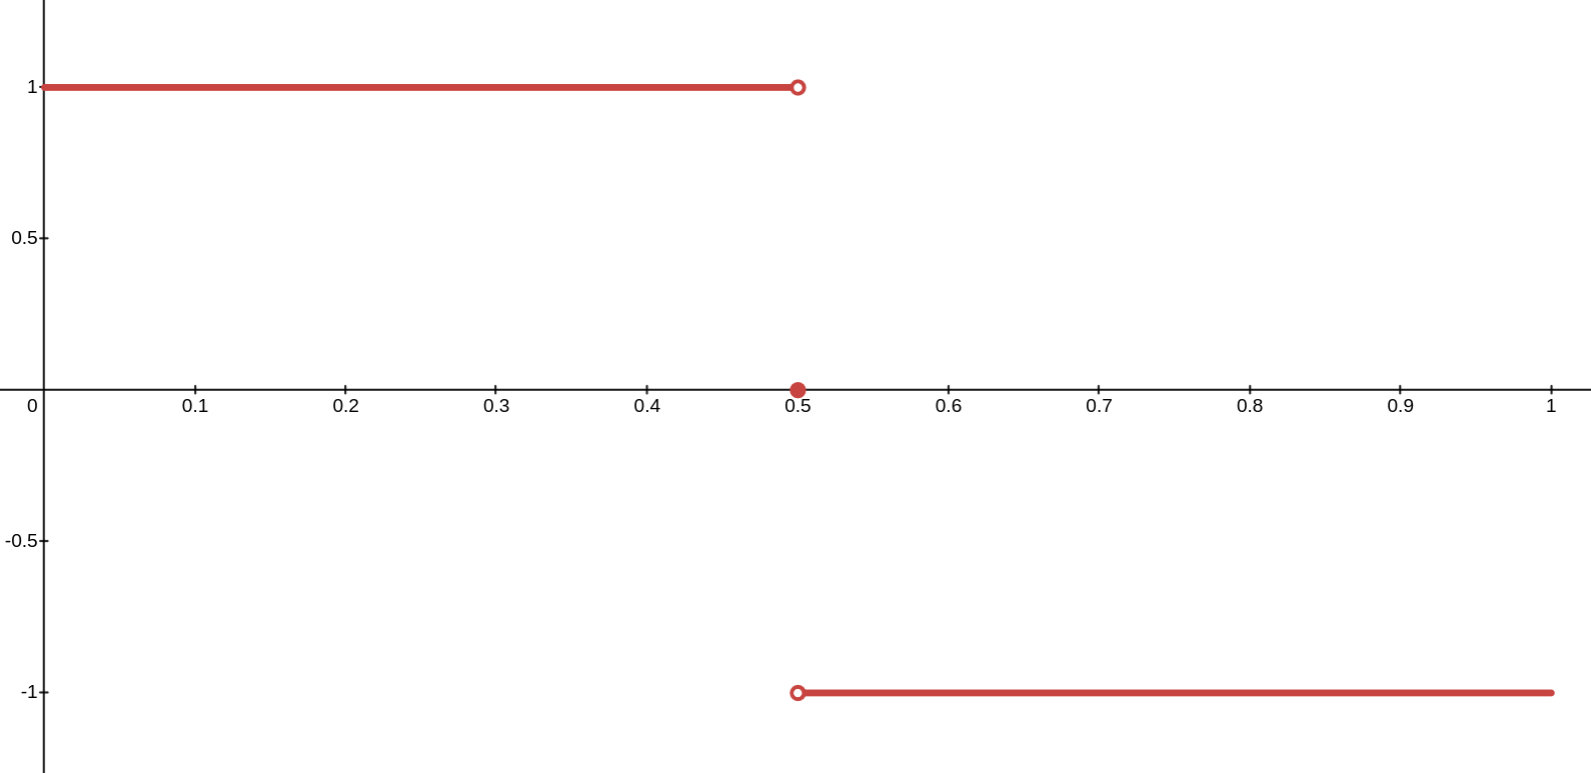
\includegraphics[width=\linewidth]{external/images/FourierEx10-1.png}
\end{image}%
\tcblower
\end{figureptx}%
Notice that this agrees with the graph of \(f^\prime\), except that \(f^\prime\) didn't exist at \(x=\frac{1}{2}\), and this series takes on the value \(0\) at \(x=\frac{1}{2}\). Notice also, that every partial sum of this series is continuous, since it is a finite combination of continuous cosine functions. This agrees with what you learned in Calculus, the (finite) sum of continuous functions is always continuous.  In the 1700s it was assumed (falsely) that this could be extended to infinite series, because every time a power series converged to a function, that function happened to be continuous.  This never failed for power series, so this example was a bit disconcerting as it is an example of the sum of infinitely many continuous functions which is, in this case, discontinuous.  Was it possible that there was some power series which converged to a function which was not continuous?  Even if there isn't, what is the difference between power series and this Fourier series?%
\par
Even more disconcerting is what happens if we  differentiate the series%
\begin{equation*}
\frac{4}{\pi}\sum_{k=0}^\infty\frac{\left(-1\right)^k}{\left(2k+1\right)} \cos\left(\left(2k+1\right)\pi x\right)
\end{equation*}
term\textendash{}by\textendash{}term as before.  Given the above graph of this series, it appears that the derivative of it should be constantly 0, except at \(x=\frac{1}{2}\), where the derivative doesn't exist. But when we perform the differentiation term\textendash{}by\textendash{}term we obtain the series%
\begin{equation*}
4\sum_{k=0}^\infty\left(-1\right)^{k+1}\sin\left(\left(2k+1\right)\pi x\right)\text{.}
\end{equation*}
and if we graph the  sum of  the first forty terms of this series, we get:         %
\begin{image}{0.125}{0.75}{0.125}{}%
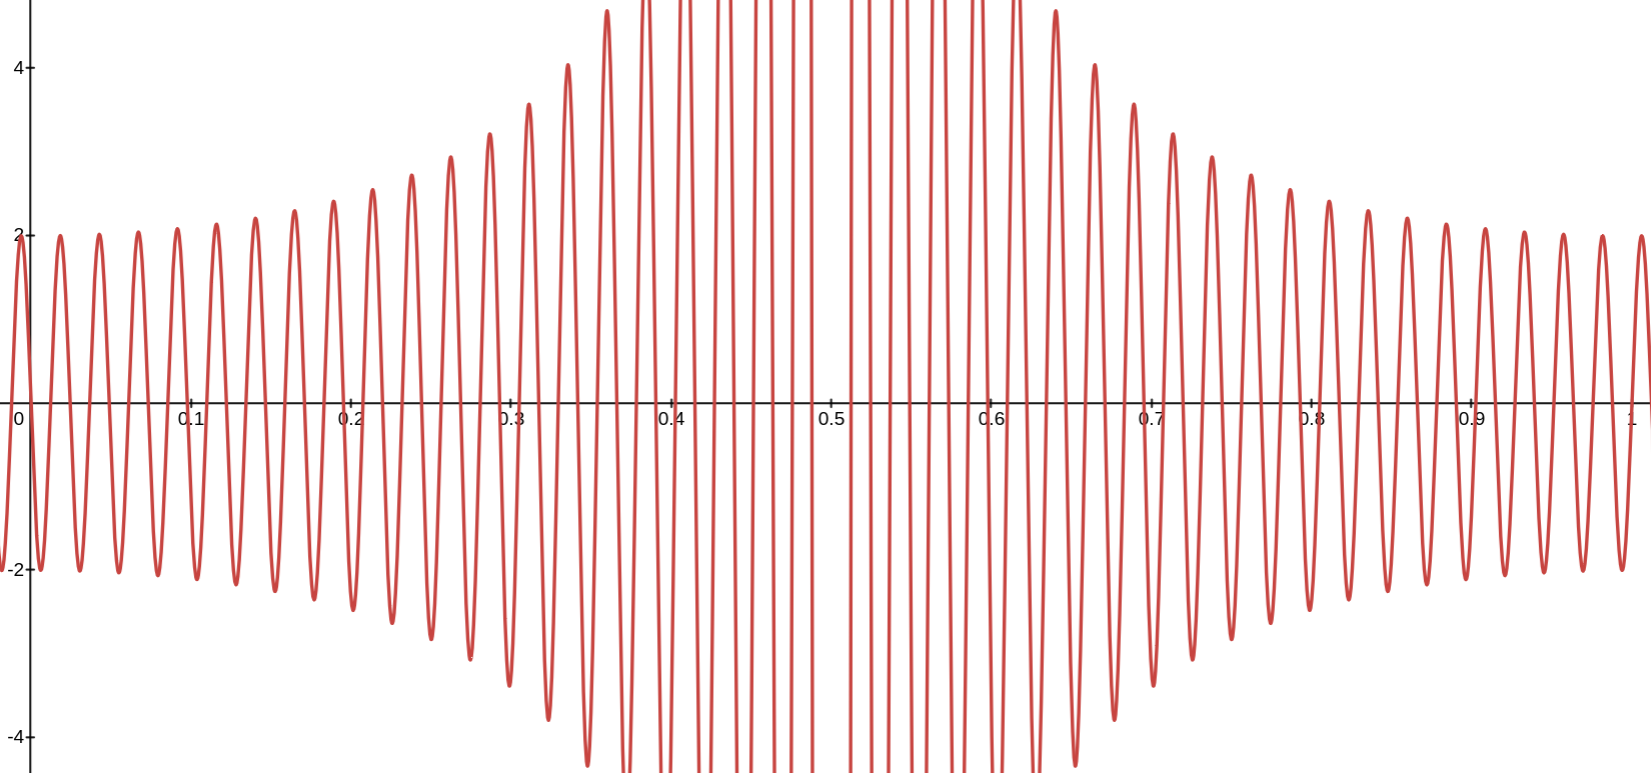
\includegraphics[width=\linewidth]{external/images/FourierEx11-1.png}
\end{image}%
We knew that there might be a problem at \(x=\frac{1}{2}\) but this is crazy! The series doesn't seem to be converging to zero at all!%
\begin{problem}{Problem}{}{prob_FourierDiverge}%
Show that when \(x=\frac{1}{4}\)%
\begin{align*}
4\sum_{k=0}^\infty\left(-1\right)^{k+1}\amp{} \sin\left(\left(2k+1\right)\pi x\right)\\
\amp{}=4\left(-\frac{1}{\sqrt{2}}+\frac{1}{\sqrt{2}}+\frac{1}{\sqrt{2}}- \frac{1}{\sqrt{2}}-\frac{1}{\sqrt{2}}+\cdots\right).
\end{align*}
%
\end{problem}
\hyperref[prob_FourierDiverge]{Problem~{\xreffont\ref{prob_FourierDiverge}}} shows that when we differentiate the series%
\begin{equation*}
\frac{4}{\pi}\sum_{k=0}^\infty\frac{\left(-1\right)^k}{\left(2k+1\right)} \cos\left(\left(2k+1\right)\pi x\right)
\end{equation*}
term by term, this differentiated series doesn't converge to anything at \(x=\frac{1}{4}\), let alone converge to zero. In this case, the old Calculus rule that the derivative of a sum is the sum of the derivatives does not apply for this infinite sum, though it did apply before. As if the continuity issue wasn't bad enough before, this was even worse. Power series were routinely differentiated and integrated term-by-term. This was part of their appeal. They were treated like ``infinite polynomials.'' Either there is some power series lurking that refuses to behave nicely, or there is some property that power series have that not all Fourier series have.%
\par
Could it be that everything we did in \hyperref[CalcIn17th18thCentury]{Chapter~{\xreffont\ref{CalcIn17th18thCentury}}} and \hyperref[PowerSeriesQuestions]{Chapter~{\xreffont\ref{PowerSeriesQuestions}}} was bogus?%
\par
Fortunately, the answer to that question is, ``No.'' Power series are generally much more well\textendash{}behaved than Fourier series.  Whenever a power series converges, the function it converges to will be continuous.  And, as long as one stays inside the interval of convergence, power series can be differentiated and integrated term\textendash{}by\textendash{}term. Power series have something going for them that your average Fourier series does not, but none of this is any more obvious to us than it was to mathematicians at the beginning of the nineteenth century.  What they did (and we do) know was that relying on intuition was perilous and that rigorous formulations were needed to either justify or dismiss these intuitions.  In some sense, the nineteenth century was the ``morning after'' the mathematical party that went on throughout the eighteenth century.%
\begin{aside}{Aside}{Convergence: Power Series vs. Fourier Series.}{Interegnum-2-40}%
We will prove all of these assertions in \hyperref[PowerSeriesRedux]{Chapter~{\xreffont\ref{PowerSeriesRedux}}}.%
\end{aside}
\begin{problem}{Problem}{}{prob_Fourier_Series-orthogonality}%
Let \(n\) and \(m\) be positive integers. Show%
\begin{equation*}
\int_{x=0}^1\cos\left(n\pi x\right)\cos\left(m\pi x\right)\dx{ x}=\left\{ \begin{matrix}0\amp \text{ if } n\neq m\\ \frac{1}{2}\amp \text{ if } n=m \end{matrix} \right.\text{.}
\end{equation*}
%
\end{problem}
\begin{problem}{Problem}{}{prob_fouriercoef}%
Use the result of \hyperref[prob_Fourier_Series-orthogonality]{Problem~{\xreffont\ref{prob_Fourier_Series-orthogonality}}} to show that if%
\begin{equation*}
f(x)=\sum_{n=1}^\infty B_n\cos\left(n\pi x\right)
\end{equation*}
on \([0,1]\), then%
\begin{equation}
B_m=2\int_{x=0}^1f(x)\cos\left(m\pi x\right)\dx{ x}.{}\label{EQUATIONCosineCoeffFourier}
\end{equation}
%
\end{problem}
\begin{problem}{Problem}{}{Interegnum-2-43}%
Apply the result of \hyperref[prob_fouriercoef]{Problem~{\xreffont\ref{prob_fouriercoef}}} to show that the Fourier cosine series of \(f(x)=x-\frac{1}{2}\) on \([0,1]\) is given by%
\begin{equation*}
\frac{-4}{\pi^2}\sum_{k=0}^\infty\frac{1}{\left(2k+1\right)^2}\cos \left((2k+1)\pi x\right)\text{.}
\end{equation*}
%
\par
Let%
\begin{equation*}
C(x,N)=\frac{-4}{\pi^2}\sum_{k=0}^N\frac{1}{\left(2k+1\right)^2}\cos
\left((2k+1)\pi x\right)
\end{equation*}
and plot \(C(x,N)\) for \(N=1,2,5,50\) \(x\in[\,0,1]\). How does this compare to the function \(f(x)=x-\frac{1}{2}\) on \([\,0,1]\)? What if you plot it for \(x\in[\,0,2]?\)%
\end{problem}
\begin{problem}{Problem}{}{Interegnum-2-44}%
\begin{enumerate}[font=\bfseries,label=(\alph*),ref=\alph*]%
\item{}Differentiate the series%
\begin{equation*}
\frac{-4}{\pi^2}\sum_{k=0}^\infty\frac{1}{\left(2k+1\right)^2}\cos \left((2k+1)\pi x\right)
\end{equation*}
term by term and plot various partial sums for that series on \([\,0,1]\).  How does this compare to the derivative of \(f(x)=x-\frac{1}{2}\) on that interval?%
\item{}Differentiate the series you obtained in part (a) and plot various partial sums of that on \([\,0,1]\).  How does this compare to the second derivative of \(f(x)=x-\frac{1}{2}\) on that interval?%
\end{enumerate}%
\end{problem}
\end{sectionptx}
\end{chapterptx}
\end{partptx}
%
%
\typeout{************************************************}
\typeout{Part III In Which We Find (Some) Answers}
\typeout{************************************************}
%
\begin{partptx}{Part}{In Which We Find (Some) Answers}{}{In Which We Find (Some) Answers}{}{}{FindingAnswers}
\renewcommand*{\partname}{Part}
%
%
\typeout{************************************************}
\typeout{Chapter 6 Convergence of Sequences and Series}
\typeout{************************************************}
%
\begin{chapterptx}{Chapter}{Convergence of Sequences and Series}{}{Convergence of Sequences and Series}{}{}{Convergence}
\renewcommand*{\chaptername}{Chapter}
%
%
\typeout{************************************************}
\typeout{Section 6.1 Sequences of Real Numbers}
\typeout{************************************************}
%
\begin{sectionptx}{Section}{Sequences of Real Numbers}{}{Sequences of Real Numbers}{}{}{SeqRealNum}
In \hyperref[CalcIn17th18thCentury]{Chapter~{\xreffont\ref{CalcIn17th18thCentury}}}, we developed the equation \(1+x+x^2+x^3+\cdots=\frac{1}{1-x}\), and we mentioned that there are  limitations to this power series representation.  For example, substituting \(x=1\) and \(x=-1\) into this expression leads to%
\begin{align*}
1+1+1+\cdots=\frac{1}{0}\amp{}\amp{} \text{and}\amp{}\amp{}  1-1+1-1+\cdots=\frac{1}{2}
\end{align*}
which are rather hard to accept.  On the other hand, if we substitute \(x=\frac{1}{2}\) into the expression we get%
\begin{equation}
1+\frac{1}{2}+\left(\frac{1}{2}\right)^2+\left(\frac{1}{2}\right)^3+\cdots=2\label{EQUATIONSeqVsSer}
\end{equation}
which seems more palatable. Until we think about it.%
\par
We can add two numbers together by the method we all learned in elementary school.  Or three numbers.  Or any finite set of numbers. At least in principle.  But infinitely many?  What does that even mean?%
\par
Before we can add infinitely many numbers together we must find a way to give meaning to the idea of adding infinitely many numbers. To do this, we examine an infinite sum by thinking of it as a \terminology{sequence} of finite \terminology{partial sums}.%
\begin{aside}{Aside}{Sequence vs. Series.}{SeqRealNum-5}%
\index{Sequence vs. Series}%
We assume that you are familiar with the distinction between a sequence and a series from your Calculus course. However, for the sake of clarity we'll make this explicit here. A \terminology{sequence} of numbers is simply a comma\textendash{}separated list of numbers. A single number from a sequence is an \terminology{element} of the sequence.  A \terminology{series} is the sum of the elements of a \terminology{sequence}.%
\par
For  example,%
\begin{equation*}
\left(1,\frac{1}{2}, \frac{1}{4}, \frac{1}{8},\cdots \right) =
\left(\frac{1}{2^n}\right)_{n=0}^\infty
\end{equation*}
is a Geometric \terminology{Sequence}, whereas%
\begin{equation*}
1+\frac{1}{2}+ \frac{1}{4}+ \frac{1}{8} + \cdots =
\sum_{n=0}^\infty \frac{1}{2^n}
\end{equation*}
is a Geometric \terminology{Series}.%
\end{aside}
From \hyperref[EQUATIONSeqVsSer]{equation~({\xreffont\ref{EQUATIONSeqVsSer}})} we would have the following \terminology{sequence} of \terminology{partial sums}.%
\begin{equation*}
\left(1,1+\frac{1}{2},1+\frac{1}{2}+\left(\frac{1}{2}\right)^2,1+
\frac{1}{2}+\left(\frac{1}{2}\right)^3,\ldots,\sum_{j=0}^n\left(\frac{1}{2}
\right)^j,\ldots\right) \text{.}
\end{equation*}
%
\par
We can plot these sums on a number line to see what they tend toward as \(n\) gets large.%
\begin{image}{0.08}{0.84}{0.08}{}%
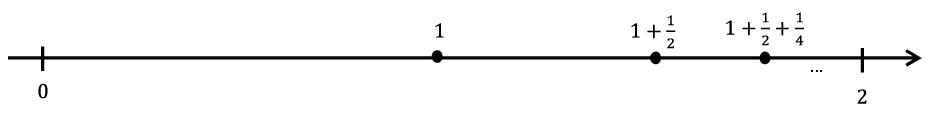
\includegraphics[width=\linewidth]{external/images/NumberLine.png}
\end{image}%
Since each partial sum is located at the midpoint between the previous partial sum and \(2\), it is reasonable to suppose that these sums tend to the number 2.  Indeed, you have probably seen an expression such as%
\begin{equation*}
\limit{n}{\infty}{\left(\sum_{j=0}^n\left(\frac{1}{2}\right)^j\right)}=2
\end{equation*}
justified by a similar argument.  Of course, relying on pictures is fine if we are satisfied with intuition.  However, to establish rigor we cannot rely on pictures or such nebulous words as ``approaches.''%
\par
No doubt you are wondering ``What's wrong with the word `approaches'?  It seems clear enough to me.'' This is often a sticking point.  But if we think carefully about what we mean by the word ``approach'' we see that there is an implicit assumption that will cause us some difficulties later if we don't expose it.%
\par
To see this consider the sequence \(\left(1,\frac12,\frac13,\frac14,\ldots\right)\).  Clearly it ``approaches'' zero, right?  But, doesn't it also ``approach'' \(-1?\) It does, in the sense that each term gets closer to \(-1\) than the one previous.  But it also ``approaches'' \(-2\), \(-3\), or even \(-1000\) in the same sense.  That's the problem with the word ``approaches.'' It just says that at each step we're closer to something than we were in the previous step.  It does not tell us that we are actually getting close.  Since the moon moves in an elliptical orbit about the earth for part of each month it is ``approaching'' the earth.  The moon gets clos\emph{er} to the earth but, thankfully, it does not get \emph{close} to the earth.%
\par
The implicit assumption we alluded to earlier is this: When we say that the sequence \(\left(\frac1n\right)_{n=1}^\infty\) ``approaches'' zero we mean that it is getting \emph{close} not clos\emph{er}.  Ordinarily this kind of vagueness in our language is pretty innocuous.  When we say ``approaches'' in casual conversation we can usually tell from the context of the conversation whether we mean ``getting close to'' or ``getting closer to.'' But when speaking mathematically we need to be more careful, more explicit, in the language we use.%
\par
So how can we change the language we use so that this ambiguity is eliminated?  We start by recognizing, rigorously, what we mean when we say that a sequence converges to zero.  For example, you would probably want to say that the sequence \(\left(1,\frac{1}{2},\frac{1}{3},\frac{1}{4},\,\ldots\right)=\left(
\frac{1}{n}\right)_{n=1}^\infty\) converges to zero.  Is there a way to give this meaning without relying on pictures or intuition?%
\par
One way would be to say that we can make \(\frac{1}{n}\) as close to zero as we wish, provided we make \(n\) large enough.  But even this needs to be made more specific.  For example, we can get \(\frac{1}{n}\) to within a distance of \(0.1\) of \(0\) provided we make \(n>10\), we can get \(\frac{1}{n}\) to within a distance of \(0.01\) of \(0\) provided we make \(n>100\), etc.  After a few such examples it is apparent that given any arbitrary distance \(\eps>0\), we can get \(\frac{1}{n}\) to within \(\eps\) of \(0\) provided we make \(n>\frac{1}{\eps}\).  This leads to the following definition.%
\begin{definition}{Definition}{Convergence to Zero of a Sequence.}{def_ConvergeToZero}%
\index{sequences!convergence to zero}\index{Definition!convergence of a sequence to zero} Let \(\left(s_n\right)=\left(s_1,s_2,s_3,\ldots\right)\) be a sequence of real numbers.  We say that \(\left(\boldsymbol{s}_{\boldsymbol{n}}\right)\) \terminology{converges to 0} and write%
\begin{equation*}
\limit{n}{\infty}{s_n}=0
\end{equation*}
provided for any \(\eps>0\), there is a real number \(N\) such that if \(n>N\), then \(|s_n|\lt \eps\).%
\end{definition}
\terminology{Notes on \hyperref[def_ConvergeToZero]{Definition~{\xreffont\ref{def_ConvergeToZero}}}}:%
\begin{enumerate}
\item{}This definition is the formal version of the idea we just talked about. Given an arbitrary distance \(\eps\), we must be able to find a specific number \(N\) such that \(s_n\) is within \(\eps\) of \(0\), whenever \(n>N\).  The \(N\) is the answer to the question, how large is ``large enough'' to put \(s_n\) this close to \(0\).%
\item{}Even though we didn't need it in the example \(\left(\frac{1}{n}\right)\), the absolute value appears in the definition because we need to make the distance from \(s_n\) to 0 smaller than \(\eps\).  Without the absolute value in the definition, we would be able to ``prove'' such outrageous statements as \(\limitt{n}{\infty}{-n}=0\), which we obviously don't want.%
\item{}The statement \(|s_n|\lt \eps\) can also be written as \(-\eps\lt s_n\lt \eps\) or \(s_n\in\left(-\eps,\eps\right)\). (See the \hyperref[prob_absolute_value]{Problem~{\xreffont\ref{prob_absolute_value}}} below.) Any one of these equivalent formulations can be used to prove convergence. Depending on the application, one of these may be more advantageous to use than the others.%
\item{}Any time an \(N\) can be found that works for a particular \(\eps\), any number \(M>N\) will work for that \(\eps\) as well, since if \(n>M\) then \(n>N\).%
\end{enumerate}
%
\begin{problem}{Problem}{}{prob_absolute_value}%
Let \(a\) and \(b\) be real numbers with \(b>0\). Prove \(|a|\lt b\) if and only if \(-b\lt a\lt b\).%
\par
Notice that this can be extended to \(\abs{a}\leq b\) if and only if \(-b\leq a\leq b\).%
\end{problem}
To illustrate how \hyperref[def_ConvergeToZero]{Definition~{\xreffont\ref{def_ConvergeToZero}}} makes the above ideas rigorous, let's use it to prove that \(\limit{n}{\infty}{\textstyle\frac{1}{n}}=0\).%
\begin{proof}{Proof}{}{SeqRealNum-19}
Let \(\eps>0\) be given. Let \(N=\frac{1}{\eps}\). If \(n>N\), then \(n>\frac{1}{\eps}\) and so \(\abs{\frac{1}{n}}=\frac{1}{n}\lt \eps\). Hence by definition, \(\limitt{n}{\infty}{\frac{1}{n}}=0\).%
\end{proof}
Notice that this proof is rigorous and makes no reference to vague notions such as ``getting smaller'' or ``approaching infinity.'' It has three components:%
\begin{enumerate}
\item{}provide the challenge of a distance \(\eps>0\),%
\item{}identify a real number \(N\), and%
\item{}show that this \(N\) works for this given \(\eps\).%
\end{enumerate}
There is also no explanation about where \(N\) came from. While it is true that this choice of \(N\) is not surprising in light of the ``scrapwork'' we did before the definition, the motivation for how we got it is not in the formal proof nor is it required.  In fact, such scrapwork is typically not included in a formal proof.  For example, consider the following.%
\begin{example}{Example}{}{SeqRealNum-21}%
Use \hyperref[def_ConvergeToZero]{Definition~{\xreffont\ref{def_ConvergeToZero}}} to prove that%
\begin{equation*}
\limit{n}{\infty}{\frac{\sin n}{n}}=0\text{.}
\end{equation*}
%
\end{example}
\begin{proof}{Proof}{}{SeqRealNum-22}
Let \(\eps>0\). Let \(N=\frac{1}{\eps}\). If \(n>N\), then \(n>\frac{1}{\eps}\) and \(\frac{1}{n}\lt \eps\). Thus \(\abs{\frac{\sin(n)}{n}}\leq\frac{1}{n}\lt \eps\). Hence by definition, \(\limitt{n}{\infty}{\frac{\sin n}{n}}=0\).%
\end{proof}
Notice that the \(N\) came out of nowhere, but you can probably see the thought process that went into this choice: We needed to use the inequality \(\abs{\sin n}\leq 1\). Again this scrapwork is not part of the formal proof, but it is typically necessary for finding what \(N\) should be. You might be able to do the next problem without doing any scrapwork first, but don't hesitate to do scrapwork if you need it.%
\begin{problem}{Problem}{}{SeqRealNum-24}%
Use \hyperref[def_ConvergeToZero]{Definition~{\xreffont\ref{def_ConvergeToZero}}}  to prove the following.%
\begin{enumerate}[font=\bfseries,label=(\alph*),ref=\alph*]%
\item{}\(\limit{n}{\infty}{\frac{1}{n^2}}=0\)%
\item{}\(\limit{n}{\infty}{\frac{1}{\sqrt{n}}}=0\)%
\end{enumerate}%
\end{problem}
\begin{example}{Example}{}{sec_defin-conv-sequ}%
In this example we'll  use \hyperref[def_ConvergeToZero]{Definition~{\xreffont\ref{def_ConvergeToZero}}} to prove%
\begin{equation*}
\limit{n}{\infty}{\frac{n+4}{n^2+1}}=0\text{.}
\end{equation*}
%
\par
As the sequences get more complicated, doing scrapwork ahead of time becomes more necessary.%
\par
\terminology{SCRAPWORK}%
\par
Given an \(\eps>0\), we need to see how large to make \(n\) in order to guarantee that \(|\frac{n+4}{n^2+1}|\lt \eps\). First notice that \(\frac{n+4}{n^2+1}\lt \frac{n+4}{n^2}\). Also, notice that if \(n>4\), then \(n+4\lt n+n=2n\). So as long as \(n>4\), we have \(\frac{n+4}{n^2+1}\lt \frac{n+4}{n^2}\lt \frac{2n}{n^2}=\frac{2}{n}\). We can make this less than \(\eps\) if we make \(n>\frac{2}{\eps}\). This means we need to make \(n>4\) and \(n>\frac{2}{\eps}\), simultaneously. These can be done if we let \(N\) be the maximum of these two numbers. This sort of thing comes up regularly, so the notation \(N=\max\left(4,\frac{2}{\eps}\right)\) was developed to mean the maximum of these two numbers. Notice that if \(N=\max\left(4, \frac{2}{\eps}\right)\) then \(N\geq 4\) and \(N\geq\frac{2}{\eps}\). We're now ready for the formal proof.%
\end{example}
\begin{proof}{Proof}{}{SeqRealNum-26}
Let \(\eps>0\). Let \(N=\max\left(4,\frac{2}{\eps}\right)\). If \(n>N\), then \(n>4\) and \(n>\frac{2}{\eps}\). Thus we have \(n>4\) and \(\frac{2}{n}\lt \eps\). Therefore%
\begin{equation*}
\abs{\frac{n+4}{n^2+1}}=\frac{n+4}{n^2+1}\lt \frac{n+4}{n^2}\lt \frac{2n}{n^2}= \frac{2}{n}\lt \eps\text{.}
\end{equation*}
%
\par
Hence by definition, \(\limit{n}{\infty}{\frac{n+4}{n^2+1}}=0\).%
\end{proof}
Again we emphasize that the scrapwork is not \alert{explicitly} a part of the formal proof.  However, if you look carefully, you can always find the scrapwork in the formal proof.%
\begin{problem}{Problem}{}{SeqRealNum-28}%
Use \hyperref[def_ConvergeToZero]{Definition~{\xreffont\ref{def_ConvergeToZero}}}  to prove that%
\begin{equation*}
\limit{n}{\infty}{\frac{n^2+4n+1}{n^3}}=0.
\end{equation*}
%
\end{problem}
\begin{problem}{Problem}{}{prob_sequences3}%
Let \(b\) be a nonzero real number with \(|b|\lt 1\) and let \(\eps>0\).%
\begin{enumerate}[font=\bfseries,label=(\alph*),ref=\alph*]%
\item{}Solve the inequality \(|b|^n\lt \eps\) for \(n\)%
\item{}Use part (a) to prove \(\limit{n}{\infty}{b^n}=0\).%
\item{}Where does your proof in part (b) break down if \(\abs{b}\ge 1\)?%
\end{enumerate}%
\end{problem}
We can negate \hyperref[def_ConvergeToZero]{Definition~{\xreffont\ref{def_ConvergeToZero}}} to prove that a particular sequence does not converge to zero. Before we look at an example, let's analyze what it means for a sequence \(\left(s_n\right)\) to not converge to zero.%
\par
Converging to zero means that any time a distance \(\eps>0\) is given, we must be able to respond with a number \(N\) such that \(|s_n|\lt \eps\) for every \(n>N\).  To have this not happen, we must be able to find some \(\eps>0\) such that no choice of \(N\) will work.  Of course, if we find such an \(\eps\), then any smaller value will also fail to have such an \(N\), but we only need one.%
\begin{example}{Example}{}{ex_zero-two-not-converge}%
Use the definition to prove that the sequence%
\begin{equation*}
\left(1+(-1)^n\right)_{n=0}^\infty=(2,0,2,0,2,\ldots)
\end{equation*}
does not converge to zero.%
\end{example}
\begin{proof}{Proof}{}{SeqRealNum-33}
If you stare at the example long enough, you see that any \(\eps\) with \(0\lt \eps\leq 2\) will cause problems. For the sake of specificity (rigor) we will let \(\eps=2\).%
\par
Also let \(N\in\RR\) be any real number. If we let \(k\) be any non\textendash{}negative integer with \(k>\frac{N}{2}\), then \(n=2k>N\), but \(|1+(-1)^n|=2\). Thus no choice of \(N\) will satisfy the conditions of the definition for this \(\eps\), (namely that \(|1+(-1)^n|\lt 2\) for all \(n>N\)) and so \(\limit{n}{\infty}{\left(1+(-1)^n\right)}\neq 0\).%
\end{proof}
\begin{problem}{Problem}{}{prob_sequences-not_converge_to_zero}%
\begin{enumerate}[font=\bfseries,label=(\alph*),ref=\alph*]%
\item{}Negate \hyperref[def_ConvergeToZero]{Definition~{\xreffont\ref{def_ConvergeToZero}}} to provide a formal definition for \(\limitt{n}{\infty}{s_n}\neq 0\).%
\item{}Use your definition from part (a) to prove \(\limitt{n}{\infty}{\frac{n}{n+100}}\neq 0\).%
\end{enumerate}%
\end{problem}
Now that we have a handle on how to rigorously prove that a sequence converges to zero, let's generalize this to a formal definition for a sequence converging to something else. Basically, we want to say that a sequence \(\left(s_n\right)\) converges to a real number \(s\), provided the difference \(\left(s_n-s\right)\) converges to zero. This leads to the following definition:%
\begin{definition}{Definition}{Convergence of a Sequence.}{def_ConvergenceOfASequence}%
\index{sequences!convergence}\index{Definition!convergence of a sequence} Let \(\left(s_n\right)=\left(s_1,s_2,s_3,\ldots\right)\) be a sequence of real numbers and let \(s\) be a real number. We say that \(\left(\boldsymbol{s}_{\boldsymbol{n}}\right)\) converges to \(\boldsymbol{s}\) and write \(\limitt{n}{\infty}{s_n}=s\) provided for any \(\eps>0\), there is a real number \(N\) such that if \(n>N\), then \(|s_n-s|\lt \eps\).%
\end{definition}
Notes on \hyperref[def_ConvergenceOfASequence]{Definition~{\xreffont\ref{def_ConvergenceOfASequence}}}%
\begin{enumerate}
\item{}Clearly \(\limit{n}{\infty}{s_n}=s\) if and only if \(\limit{n}{\infty}{\left(s_n-s\right)}=0\).       %
\item{}Again notice that this says that we can make \(s_n\) as close to \(s\) as we wish (within \(\eps\)) by making \(n\) large enough (\(>N)\). As before, this definition makes these notions very specific.%
\item{}Notice that \(\abs{s_n-s}\lt \eps\) can be written in the following equivalent forms%
\par
%
\begin{itemize}[label=\textbullet]
\item{}\(\displaystyle \abs{s_n-s}\lt \eps\)%
\item{}\(\displaystyle -\eps\lt s_n-s\lt \eps\)%
\item{}\(\displaystyle s-\eps\lt s_n\lt s+\eps\)%
\item{}\(\displaystyle s_n\in\left(s-\eps,s+\eps\right)\)%
\end{itemize}
%
\par
and we are free to use any one of these which is convenient at the time.%
\end{enumerate}
%
\begin{aside}{Aside}{Double Implication.}{SeqRealNum-38}%
The phrase ``if and only if'' (seen in item 1 above) is a term of art in mathematics. The symbol ``\(\Leftrightarrow \)'' is equivalent.%
\par
Formally it means that each statement follows logically from the other. If you are asked to prove the statement%
\begin{equation*}
A\Leftrightarrow B
\end{equation*}
you need to first assume that \(A\) is true to prove \(B\). Then you assume that \(B\) is true to prove \(A\).%
\par
In a classroom setting it is often abbreviated as ``iff.''%
\end{aside}
As an example, let's use this definition to prove that the sequence in part (b) of \hyperref[prob_sequences-not_converge_to_zero]{Problem~{\xreffont\ref{prob_sequences-not_converge_to_zero}}} converges to \(1\).%
\begin{example}{Example}{}{example_SeriesConverge}%
Prove \(\limitt{n}{\infty}{\frac{n}{n+100}}=1\).%
\par
\terminology{SCRAPWORK}%
\par
Given an \(\eps>0\), we need to get \(\abs{\frac{n}{n+100}-1}\lt \eps\). This prompts us to do some algebra.%
\begin{equation*}
\left|\frac{n}{n+100}-1\right|=\left|\frac{n-(n+100)}{n+100}\right|\leq\frac{100}{n}\text{.}
\end{equation*}
%
\par
This in turn, seems to suggest that \(N=\frac{100}{\eps}\) should work.%
\end{example}
\begin{proof}{Proof}{}{SeqRealNum-41}
Let \(\eps>0\). Let \(N=\frac{100}{\eps}\). If \(n>N\), then \(n>\frac{100}{\eps}\) and so \(\frac{100}{n}\lt \eps\). Hence%
\begin{equation*}
\left|\frac{n}{n+100}-1\right|=\left|\frac{n-(n+100)}{n+100}\right|= \frac{100}{n+100}\lt \frac{100}{n}\lt \eps\text{.}
\end{equation*}
%
\par
Thus by definition \(\limitt{n}{\infty}{\frac{n}{n+100}} =1\).%
\end{proof}
Notice again that the scrapwork is not part of the formal proof and the author of a proof is not obligated to explain where the choice of \(N\) came from (although the thought process can usually be seen in the formal proof).  The formal proof contains only these requisite three parts:%
\begin{itemize}[label=\textbullet]
\item{}provide the challenge of an arbitrary \(\eps>0\),%
\item{}provide a specific \(N\), and%
\item{}show that this \(N\) works for the given \(\eps\).%
\end{itemize}
%
\par
Also notice that given a specific sequence such as \(\left(\frac{n}{n+100}\right)\), the definition does not indicate what the limit would be if in fact, it exists.  Once an educated guess is made the definition only verifies that this intuition is correct.%
\par
This leads to the following question: If intuition is needed to determine what a limit of a sequence should be, then what is the purpose of this relatively non\textendash{}intuitive, complicated definition?%
\par
Remember that when these rigorous formulations were developed, intuitive notions of convergence were already in place and had been used with great success.  But the arguments based on them could not be fully justified. This definition was developed to address the foundational issues, not to help us compute limits.%
\par
Could our intuitions be verified in a concrete fashion that was above reproach? This was the purpose of this non-intuitive definition. It was to be used to verify that our intuition was, in fact, correct and do so in a very prescribed manner. For example, if \(b>0\) is a fixed number, then you would probably say as \(n\) approaches infinity, \(b^{\left(\frac{1}{n}\right)}\) approaches \(b^0=1\). After all, we did already prove that \(\limit{n}{\infty}{\frac{1}{n}}=0\). We should be able to back up this intuition with our rigorous definition.%
\begin{problem}{Problem}{}{SeqRealNum-47}%
\index{limit!\(\limit{n}{\infty}{b^{\left(\frac{1}{n}\right)}}=1\) if \(b>0\)} Let \(b>0\).  Use \hyperref[def_ConvergenceOfASequence]{Definition~{\xreffont\ref{def_ConvergenceOfASequence}}} to prove \(\limitt{n}{\infty}{b^{\left(\frac{1}{n}\right)}}=1\).%
\par\smallskip%
\noindent\textbf{\blocktitlefont Hint}.\hypertarget{SeqRealNum-47-2}{}\quad{}You will probably need to separate this into three cases: \(0\lt b\lt 1\), \(b=0\), and \(b\gt 1\).%
\end{problem}
\begin{problem}{Problem}{}{prob_series-geometric}%
\begin{enumerate}[font=\bfseries,label=(\alph*),ref=\alph*]%
\item{}Prove that if \(x\neq 1\), then%
\begin{equation*}
1+x+x^2+\cdots+x^n=\frac{1-x^{n+1}}{1-x}\text{.}
\end{equation*}
%
\item{}Use (a) to prove that if \(|x|\lt 1\), then \(\limit{n}{\infty}{\left(\sum_{j=0}^nx^j\right)}=\frac{1}{1-x}\).%
\end{enumerate}%
\end{problem}
\begin{problem}{Problem}{}{SeqRealNum-49}%
\begin{enumerate}[font=\bfseries,label=(\alph*),ref=\alph*]%
\item{}Provide a rigorous definition for \(\limitt{n}{\infty}{s_n}\neq s\).%
\item{}Use your definition from part (a) to show that for any real number \(a\), \(\limitt{n}{\infty}{\left(\left(-1\right)^n\right)}\neq a\).%
\par\smallskip%
\noindent\textbf{\blocktitlefont Hint}.\hypertarget{SeqRealNum-49-4-2}{}\quad{}Choose \(\eps=1\) and use the fact that \(\abs{a-(-1)^n}\lt 1\) is equivalent to \(\left(-1\right)^n-1\lt a\lt \left(-1\right)^n+1\) to show that no choice of \(N\) will work for this \(\eps\).%
\end{enumerate}%
\end{problem}
\begin{problem}{Problem}{}{SeqRealNum-50}%
Prove that if \(\limit{n}{\infty}{s_n}=s\) then \(\limit{n}{\infty}{\abs{s_n}}=\abs{s}\).  Prove that the converse is true when \(s=0\), but it is not necessarily true otherwise.%
\end{problem}
\begin{problem}{Problem}{}{SeqRealNum-51}%
\begin{enumerate}[font=\bfseries,label=(\alph*),ref=\alph*]%
\item{}Let \(\left(s_n\right)\) and \(\left(t_n\right)\) be sequences with \(s_n\leq t_n,\forall\  n\).  Suppose \(\limit{n}{\infty}{s_n}=s\) and \(\limit{n}{\infty}{t_n}=t\). Prove \(s\leq t\).%
\par\smallskip%
\noindent\textbf{\blocktitlefont Hint}.\hypertarget{SeqRealNum-51-2-2}{}\quad{}Assume for contradiction, that \(s>t\) and use the definition of convergence with \(\eps=\frac{s-t}{2}\) to produce an \(n\) with \(s_n>t_n\).%
\item{}Prove that if a sequence converges, then its limit is unique.  That is, prove that if \(\limit{n}{\infty}{s_n}=s\) and \(\limit{n}{\infty}{s_n}=t\), then \(s=t\).%
\end{enumerate}%
\end{problem}
\begin{problem}{Problem}{}{SeqRealNum-52}%
Prove that if \(\limit{n}{\infty}{s_n}=s\) and \(\limit{n}{\infty}{\left(s_n-t_n\right)}=0\), then \(\limit{n}{\infty}{t_n}=s\).%
\end{problem}
\begin{problem}{Problem}{}{SeqRealNum-53}%
\begin{enumerate}[font=\bfseries,label=(\alph*),ref=\alph*]%
\item{}Prove that if \(\limit{n}{\infty}{s_n}=s\) and \(s\lt
t\), then there exists a real number \(N\) such that if \(n>N\) then \(s_n\lt t\).%
\item{}Prove that if \(\limit{n}{\infty}{s_n}=s\) and \(r\lt
s\), then there exists a real number \(M\) such that if \(n>M\) then \(r\lt s_n\).%
\end{enumerate}%
\end{problem}
\begin{problem}{Problem}{The Ratio Test.}{prob_RatioTest}%
Suppose \(\left(s_n\right)\) is a sequence of positive numbers such that%
\begin{equation*}
\limit{n}{\infty}{\left(\frac{s_{n+1}}{s_n}\right)}=L\text{.}
\end{equation*}
%
\begin{enumerate}[font=\bfseries,label=(\alph*),ref=\alph*]%
\item{}Prove that if \(L\lt 1\), then \(\limit{n}{\infty}{s_n}=0\).%
\par\smallskip%
\noindent\textbf{\blocktitlefont Hint}.\hypertarget{prob_RatioTest-4-2}{}\quad{}Choose \(R\) with \(L\lt R\lt 1\).  By the previous problem, \(\exists\) \(N\) such that if \(n>N\), then \(\frac{s_{n+1}}{s_n}\lt R\).  Let \(n_0>N\) be fixed and show \(s_{n_0+k}\lt R^ks_{n_0}\). Conclude that \(\limit{k}{\infty}{s_{n_0+k}}=0\) and let \(n=n_0+k\).%
\item{}Let \(c\) be a positive real number.  Prove \(\limit{n}{\infty}{\left(\frac{c^n}{n!}\right)}=0\).%
\end{enumerate}%
\end{problem}
\end{sectionptx}
%
%
\typeout{************************************************}
\typeout{Section 6.2 The Limit as a Primary Tool}
\typeout{************************************************}
%
\begin{sectionptx}{Section}{The Limit as a Primary Tool}{}{The Limit as a Primary Tool}{}{}{LimitAsPrimary}
As you saw in the \hyperref[SeqRealNum]{previous section} the formal definition of the convergence of a sequence is meant to capture rigorously our intuitive understanding of convergence.  However, the definition itself is an unwieldy tool. If only there were some way to be rigorous without having to run back to the definition each time.  Fortunately, there is a way.  If we can use the definition to prove some general rules about limits then we could use these rules whenever they apply and be assured that everything was still rigorous.  A number of these should look familiar from Calculus.%
\begin{problem}{Problem}{Limit of a Constant Sequence is the Constant.}{PROBLEMLimConst}%
Let \(\left(c\right)_{n=1}^\infty=(c,c,c,\ldots)\) be a constant sequence.  Show that \(\limitt{n}{\infty}{c}=c\).%
\end{problem}
In proving the familiar limit theorems, the following will be a very useful tool.%
\begin{lemma}{Lemma}{}{}{Tri-RevTri-Ineq}%
\index{Triangle Inequalities}%
\index{Triangle Inequalities!Triangle Inequality}%
\index{Triangle Inequalities!Reverse Triangle Inequalitiy}%
%
\begin{descriptionlist}
\begin{dlimedium}{Triangle Inequality:}{TriangleIneq}%
Let \(a\) and \(b\) be real numbers. Then%
\begin{equation*}
\abs{a+b}\leq \abs{a}+\abs{b}\text{.}
\end{equation*}
%
\end{dlimedium}%
\begin{dlimedium}{Reverse Triangle Inequality:}{InvTriangleIneq}%
Let \(a\) and \(b\) be real numbers. Then%
\begin{equation*}
\abs{a}-\abs{b}\leq\abs{a-b}
\end{equation*}
%
\end{dlimedium}%
\end{descriptionlist}
%
\end{lemma}
\begin{problem}{Problem}{}{Tri-RevTri-Ineq_prob}%
\begin{enumerate}[font=\bfseries,label=(\alph*),ref=\alph*]%
\item{}Prove \hyperref[Tri-RevTri-Ineq]{Lemma~{\xreffont\ref{Tri-RevTri-Ineq}}}.%
\par\smallskip%
\noindent\textbf{\blocktitlefont Hint}.\hypertarget{Tri-RevTri-Ineq_prob-2-2}{}\quad{}For the Reverse Triangle Inequality, consider \(\abs{a}=\abs{a-b+b}\).%
\item{}Show \(\Big||a|-|b|\Big|\leq|a-b|\).%
\par\smallskip%
\noindent\textbf{\blocktitlefont Hint}.\hypertarget{Tri-RevTri-Ineq_prob-3-2}{}\quad{}You want to show that%
\begin{equation*}
|a|-|b|\leq|a-b|
\end{equation*}
and that%
\begin{equation*}
-\left(|a|-|b|\right)\leq|a-b|\text{.}
\end{equation*}
%
\end{enumerate}%
\end{problem}
\begin{theorem}{Theorem}{Limit of a Sum of Sequences is the Sum of the Limits.}{}{thm_SumOfSequences}%
\index{limit!of a sum of sequences}%
If \(\limitt{n}{\infty}{a_n}=a\) and \(\limitt{n}{\infty}{b_n}=b\), then%
\begin{equation*}
\limit{n}{\infty}{\left(a_n+b_n\right)}=a+b\text{.}
\end{equation*}
%
\end{theorem}
We  often state this theorem informally as ``the limit of a sum is the sum of the limits.'' However, to be absolutely precise, what it says is that if we already know that two sequences converge, then the sequence formed by summing their corresponding terms  will also converge and in fact, it will converge to the sum of those individual limits.%
\par
We'll provide the scrapwork and leave the formal write\textendash{}up to you in \hyperref[PROBLEMLimitOfSum]{Problem~{\xreffont\ref{PROBLEMLimitOfSum}}}. Be sure you justify every step. Also, note the role of the \hyperref[Tri-RevTri-Ineq]{triangle inequality} in the proof.%
\par
\terminology{SCRAPWORK:}%
\par
If we let \(\eps>0\), then we want to find \(N\) such that if \(n>N\), then \(\abs{\left(a_n+b_n\right)-\left(a+b\right)}\lt \eps\). Since we know that \(\limit{n}{\infty}{a_n}=a\) and \(\limit{n}{\infty}{b_n}=b\), we can make \(\abs{a_n-a}\) and \(\abs{b_n-b}\) as small as we wish, provided we make \(n\) large enough.  Let's look closely at our goal to see if we can close the gap between what we know and what we want.  We know, by the triangle inequality, that%
\begin{equation*}
\abs{\left(a_n+b_n\right)-\left(a+b\right)}=\abs{\left(a_n-a\right)+\left(b_n-b\right)}\leq\abs{a_n-a}+\abs{b_n-b}\text{.}
\end{equation*}
To make this whole thing less than \(\eps\), it makes sense to make each part less than \(\frac{\eps}{2}\).%
\par
Fortunately, we can do that as the definitions of \(\limit{n}{\infty}{a_n}=a\) and \(\limit{n}{\infty}{b_n}=b\) allow us to make \(\abs{a_n-a}\) and \(\abs{b_n-b}\) arbitrarily small.%
\par
Specifically, since \(\limit{n}{\infty}{a_n}=a\), there exists an \(N_1\) such that if \(n>N_1\) then \(\abs{a_n-a}\lt \frac{\eps}{2}\).  Also since \(\limit{n}{\infty}{b_n}=b\), there exists an \(N_2\) such that if \(n>N_2\) then \(\abs{b_n-b}\lt
\frac{\eps}{2}\).  Since we want both of these to occur, it makes sense to let \(N=\)max\(\left(N_1,N_2\right)\).  This should be the \(N\) that we seek.%
\begin{problem}{Problem}{}{PROBLEMLimitOfSum}%
Prove \hyperref[thm_SumOfSequences]{Theorem~{\xreffont\ref{thm_SumOfSequences}}}.%
\end{problem}
\begin{theorem}{Theorem}{Limit of the Product of Sequences is the Product of the Limits.}{}{thm_LimitOfProduct}%
\index{limit!of a product of sequences}%
\index{limit!products of}%
If \(\limit{n}{\infty}{a_n}=a\) and \(\limit{n}{\infty}{b_n}=b\), then \(\limit{n}{\infty}{\left(a_n b_n\right)}=a b\).%
\end{theorem}
\terminology{SCRAPWORK:} Given \(\eps>0\), we want \(N\) so that if \(n>N\), then \(\abs{a_n  b_n-a  b}\lt \eps\). One of the standard tricks in analysis is to ``uncancel.'' In this case we will subtract and add a convenient term. Normally these would ``cancel out,'' which is why we say that we will uncancel to put them back in. You already saw an example of this in proving the Reverse Triangle Inequality (\hyperref[Tri-RevTri-Ineq_prob]{Problem~{\xreffont\ref{Tri-RevTri-Ineq_prob}}}). In the present case, consider%
\begin{align*}
\abs{a_n  b_n-a  b}\amp =\abs{a_n  b_n-a_n b+a_n b-a  b}\\
\amp \leq \abs{a_n  b_n-a_n  b}+\abs{a_n b-a b}|\\
\amp =\abs{a_n}\abs{b_n-b}+\abs{b}\abs{a_n-a}\text{.}
\end{align*}
%
\par
We can make this whole thing less than \(\eps\), provided we make each term in the sum less than \(\frac{\eps}{2}\).  We can make \(\big|b\big|\big|a_n-a\big|\lt \frac{\eps}{2}\) if we make \(\big|a_n-a\big|\lt \frac{\eps}{2|b|}\).%
\par
But wait! What if \(b=0\)?%
\par
We could handle this as a separate case or we can do the following ``slick trick.'' Notice that we can add one more line to the above string of inequalities:%
\begin{equation*}
\left|a_n\right|\left|b_n-b\right|+\left|b\right|\left|a_n-a\right|\lt
\left|a_n
\right|\left|b_n-b\right|+\left(\left|b\right|+1\right)\left|a_n-a
\right|\text{.}
\end{equation*}
Now we can make \(\left|a_n-a\right|\lt
\frac{\eps}{2\left(|b|+1\right)}\) and not worry about dividing by zero.%
\par
Making \(\abs{a_n}\abs{b_n-b}\lt \frac{\eps}{2}\) requires a bit more finesse. At first glance, one would be tempted to try and make \(\abs{b_n-b}\lt \frac{\eps}{2|a_n|}\). Even if we ignore the fact that we could be dividing by zero (which we could handle), we have a bigger problem. According to the definition of \(\limitt{n}{\infty}{b_n}=b\), we can make \(\abs{b_n-b}\) smaller than any given fixed positive number, as long as we make \(n\) large enough (larger than some \(N\) which goes with a given epsilon). Unfortunately, \(\frac{\eps}{2|a_n|}\) is not fixed as it has the variable \(n\) in it; there is no reason to believe that a single \(N\) will work with all possible values of \(n\) simultaneously. To handle this impasse, we need the following:%
\begin{lemma}{Lemma}{}{}{lemma_BoundedConvergent}%
\index{sequences!convergence!convergent sequences are bounded}%
\alert{A Convergent Sequence Is Bounded.}%
\par
If \(\limitt{n}{\infty}{a_n}=a\), then there exists \(B>0\) such that \(\abs{a_n}\leq B\) for all \(n\).%
\end{lemma}
\begin{problem}{Problem}{}{prob_BoundedConvergent}%
Prove \hyperref[lemma_BoundedConvergent]{Lemma~{\xreffont\ref{lemma_BoundedConvergent}}}.%
\par\smallskip%
\noindent\textbf{\blocktitlefont Hint}.\hypertarget{prob_BoundedConvergent-3}{}\quad{}We know that there exists \(N\) such that if \(n>N\), then \(\abs{a_n-a}\lt 1\).  Let \(B=\)max\(\left(\abs{a_1},\abs{a_2},\ldots,\abs{a_{\lceil{N}\rceil}},\abs{a}+1\right)\), where \(\lceil{N}\rceil\) represents the smallest integer greater than or equal to \(N\).%
\end{problem}
Armed with \hyperref[lemma_BoundedConvergent]{Lemma~{\xreffont\ref{lemma_BoundedConvergent}}} we can add the following inequality to the scrapwork above.%
\begin{align*}
\abs{a_n\cdot b_n-a\cdot b}\amp =\abs{a_n\cdot b_n-a_n\cdot b+a_n\cdot b-a\cdot b}\\
\amp \leq \abs{a_n\cdot b_n-a_n\cdot b}+ \abs{a_n\cdot b-a\cdot b}\\
\amp = \abs{a_n}\abs{b_n-b}+\abs{b}\abs{a_n-a}\\
\amp \lt B \abs{b_n-b}+\left(\abs{b}+1\right)\abs{a_n-a}.
\end{align*}
%
\par
At this point, we should be able to make the last line of this less than \(\eps\).%
\par
\terminology{END OF SCRAPWORK}%
\begin{problem}{Problem}{}{LimitAsPrimary-26}%
Prove \hyperref[thm_LimitOfProduct]{Theorem~{\xreffont\ref{thm_LimitOfProduct}}}.%
\end{problem}
\begin{corollary}{Corollary}{(to Theorem~{\xreffont\ref*{thm_LimitOfProduct}}).}{}{cor_1}%
If \(\limit{n}{\infty}{a_n}=a\) and \(c\in\mathbb{R}\), then \(\limit{n}{\infty}{c\cdot a_n}=c\cdot a\).%
\end{corollary}
\begin{problem}{Problem}{}{LimitAsPrimary-28}%
Prove  \hyperref[cor_1]{Corollary~{\xreffont\ref{cor_1}}}.%
\end{problem}
The following theorem is the analog of \hyperref[thm_LimitOfProduct]{Theorem~{\xreffont\ref{thm_LimitOfProduct}}} for quotients.%
\begin{theorem}{Theorem}{Limit of the Quotient of Sequences is the Quotient of the Limits.}{}{thm_LimitOfQuotient}%
\index{limit!of a quotient of sequences}%
Suppose \(\limitt{n}{\infty}{a_n}=a\) and \(\limitt{n}{\infty}{b_n}=b\). Also suppose \(b\neq 0\) and \(b_n\neq 0, \forall n\).%
\par
Then%
\begin{equation*}
\limit{n}{\infty}{\left(\frac{a_n}{b_n}\right)}=\frac{a}{b}\text{.}
\end{equation*}
%
\end{theorem}
\begin{problem}{Problem}{}{LimitAsPrimary-31}%
Prove \hyperref[thm_LimitOfQuotient]{Theorem~{\xreffont\ref{thm_LimitOfQuotient}}}.%
\par
\terminology{SCRAPWORK}%
\par
It is helpful to look first at the special case%
\begin{equation*}
\limitt{n}{\infty}{\left(\frac{1}{b_n}\right)}=\frac{1}{b}\text{.}
\end{equation*}
The general case will follow from this and from \hyperref[thm_LimitOfProduct]{Theorem~{\xreffont\ref{thm_LimitOfProduct}}}.%
\par
Consider \(\big|\frac{1}{b_n}-\frac{1}{b}\big|=\frac{|b-b_n|}{|b_n||b|}\). We are faced with the same dilemma we had when we were proving \hyperref[thm_LimitOfProduct]{Theorem~{\xreffont\ref{thm_LimitOfProduct}}}; we need to get \(\big|\frac{1}{b_n}\big|\) bounded above. This means we need to get \(\abs{b_n}\) bounded away from zero (at least for large enough \(n\)).%
\par
This can be done as follows. Since \(b\neq 0\), then \(\frac{|b|}{2}>0\). Thus, by the definition of \(\limit{n}{\infty}{b_n}=b\) there exists \(N_1\) such that if \(n>N_1\), then \(\abs{b}-\abs{b_n}\leq\big|b-b_n\big|\lt \frac{\abs{b}}{2}\). Thus when \(n>N_1\), \(\frac{\abs{b}}{2}\lt \abs{b_n}\) and so \(\frac{1}{\abs{b_n}}\lt \frac{2}{\abs{b}}\). This says that for \(n>N_1\), \(\frac{\abs{b-b_n}}{\abs{b_n}\abs{b}}\lt \frac{2}{\abs{b}^2}\abs{b-b_n}\). We should be able to make this smaller than a given \(\eps>0\), provided we make \(n\) large enough.%
\end{problem}
The results of \hyperref[PROBLEMLimConst]{Problem~{\xreffont\ref{PROBLEMLimConst}}}, \hyperref[thm_SumOfSequences]{Theorem~{\xreffont\ref{thm_SumOfSequences}}}, \hyperref[thm_LimitOfProduct]{Theorem~{\xreffont\ref{thm_LimitOfProduct}}}, and \hyperref[thm_LimitOfQuotient]{Theorem~{\xreffont\ref{thm_LimitOfQuotient}}} allow us to find the limits of complicated sequences and then rigorously verify that these are in fact, the correct limits without resorting to the definition of a limit.%
\begin{problem}{Problem}{}{LimitAsPrimary-33}%
\begin{enumerate}[font=\bfseries,label=(\alph*),ref=\alph*]%
\item{}Use the  theorems from this section  to prove that%
\begin{equation*}
\limit{n}{\infty}{\frac{3n^3-100n+1}{5n^3+4n^2-7}} =
\limit{n}{\infty}{\frac{n^3\left(3-\frac{100}{n^2}+\frac{1}{n^3}\right)}{n^3
\left(5+\frac{4}{n}-\frac{7}{n^3}\right)}}=\frac{3}{5}\text{.}
\end{equation*}
%
\item{}Prove that%
\begin{equation*}
\limit{n}{\infty}{\frac{a_0+a_1n+a_2n^2+
\cdots+a_kn^k}{b_0+b_1n+b_2n^2+\cdots+b_kn^k}}=\frac{a_k}{b_k}\text{,}
\end{equation*}
provided \(b_k\neq 0\).%
\par
Be sure to explain why division by zero is not an issue. (See the hint.)%
\par\smallskip%
\noindent\textbf{\blocktitlefont Hint}.\hypertarget{LimitAsPrimary-33-4-2}{}\quad{}A polynomial only has finitely many roots.%
\end{enumerate}%
\end{problem}
There is one more theorem which  will prove to be a valuable tool.%
\begin{theorem}{Theorem}{The Squeeze Theorem for Sequences.}{}{thm_SqueezeTheorem}%
\index{limit!Squeeze Theorem for Sequences}%
%
\par
Let \(\left(r_n\right),\left(s_n\right)\), and \(\left(t_n\right)\) be sequences of real numbers with \(r_n\leq s_n\leq t_n,\forall\) positive integers \(n\). Suppose \(\limit{n}{\infty}{r_n}=s=\limit{n}{\infty}{t_n}\). Then \(\left(s_n\right)\) must converge and \(\limit{n}{\infty}{s_n}=s\).%
\end{theorem}
\begin{problem}{Problem}{}{LimitAsPrimary-36}%
Prove the \hyperref[thm_SqueezeTheorem]{Squeeze Theorem for Sequences}.%
\par\smallskip%
\noindent\textbf{\blocktitlefont Hint}.\hypertarget{LimitAsPrimary-36-3}{}\quad{}This is probably a place where you would want to use \(s-\eps\lt s_n\lt s+\eps\) instead of \(|s_n-s|\lt
\eps\).%
\end{problem}
The Squeeze Theorem is true even if \(r_n\leq s_n\leq
t_n\) only holds for sufficiently large \(n\); i.e., for \(n\) larger than some fixed \(N_0\).  This is true because when you find an \(N_1\) that works in the original proof, this can be modified by choosing \(N=\)max\(\left(N_0,N_1\right)\).  Also note that this theorem really says two things:%
\begin{enumerate}
\item{}\(\left(s_n\right)\) converges, and%
\item{}it converges to \(s\).%
\end{enumerate}
This subtle point affects how one should properly use the Squeeze Theorem.%
\begin{example}{Example}{}{example_SqzeEx}%
Prove \(\limit{n}{\infty}{\frac{n+1}{n^2}}=0\).%
\end{example}
\begin{proof}{Proof}{}{LimitAsPrimary-39}
Notice that \(0\leq\frac{n+1}{n^2}\leq\frac{n+n}{n^2}=\frac{2}{n}\). Since \(\limit{n}{\infty}{0}=0=\limit{n}{\infty}{\frac{2}{n}}\), then by the Squeeze Theorem, \(\limit{n}{\infty}{\frac{n+1}{n^2}}=0\).%
\end{proof}
Our proof in \hyperref[example_SqzeEx]{Example~{\xreffont\ref{example_SqzeEx}}} is completely rigorous and is the proper way to use the \hyperref[thm_SqueezeTheorem]{Squeeze Theorem}.%
\par
Next we give an example of an improper use of the Squeeze Theorem. It is easy to fall into this error. Be careful.%
\begin{example}{Example}{How Not to Use the Squeeze Theorem.}{EXAMPLENotUseSquzTheorem}%
Look again at  \hyperref[example_SqzeEx]{Example~{\xreffont\ref{example_SqzeEx}}}. Notice that%
\begin{equation*}
0\leq\frac{n+1}{n^2}\leq\frac{n+n}{n^2}=\frac{2}{n}\text{,}
\end{equation*}
so%
\begin{equation*}
0=\limit{n}{\infty}{0} \leq \limit{n}{\infty}{\frac{n+1}{n^2}}\leq\limit{n}{\infty}{\frac{2}{n}}=0
\end{equation*}
and%
\begin{equation*}
\limit{n}{\infty}{\frac{n+1}{n^2}}=0\text{.}
\end{equation*}
%
\par
This is incorrect in form because it presumes that \(\limitt{n}{\infty}{\frac{n+1}{n^2}}\) exists, which we don't yet know. If we knew that the limit existed to begin with, then this would be fine. The Squeeze Theorem proves that the limit does in fact exist, but it must be so stated.%
\end{example}
\begin{problem}{Problem}{}{LimitAsPrimary-43}%
Prove that if the sequence \(\left(s_n\right)\) is bounded then%
\begin{equation*}
\limit{n}{\infty}{\left(\frac{s_n}{n}\right)}=0\text{.}
\end{equation*}
%
\end{problem}
The general theorems we have seen in this section will allow us to rigorously explore convergence of power series in the next chapter without appealing directly to the definitions.  However there will still be times when we will need to apply the definition directly.%
\par
But before we go into that let's examine divergence a bit more closely.%
\end{sectionptx}
%
%
\typeout{************************************************}
\typeout{Section 6.3 Divergence}
\typeout{************************************************}
%
\begin{sectionptx}{Section}{Divergence}{}{Divergence}{}{}{DivergentSeq}
In \hyperref[thm_rearrangements]{Theorem~{\xreffont\ref{thm_rearrangements}}} we saw that there is a rearrangment of the alternating Harmonic series which diverges to \(\infty\) or \(-\infty\). In that section we did not fuss over any formal notions of divergence. We assumed instead that you are already familiar with the concept of divergence, probably from taking Calculus in the past.%
\par
However we are now in the process of building precise, formal definitions for the concepts we will be using so we define the divergence of a sequence as follows.%
\begin{definition}{Definition}{}{thm_divergence_of_a_sequence}%
\index{sequences!divergence of}%
\index{divergence!of a sequence}%
A sequence of real numbers \(\left(s_n\right)_{n=1}^\infty\) diverges if it does not converge to any \(a\in\RR\).%
\end{definition}
It may seem unnecessarily pedantic of us to insist on formally stating such an obvious definition. After all ``converge'' and ``diverge'' are opposites in ordinary English. Why wouldn't they be mathematically opposite too? Why do we have to go to the trouble of formally defining both of them? Since they are opposites defining one implicitly defines the other doesn't it?%
\par
One way to answer that criticism is to state that in mathematics we \emph{always} work from precisely stated definitions and tightly reasoned logical arguments.%
\par
But this is just more pedantry. It is a way of saying, ``Because we said so'' all dressed up in imposing language. We need to do better than that.%
\par
One reason for providing formal definitions of both convergence and divergence is that in mathematics we frequently co-opt words from natural languages like English and imbue them with mathematical meaning that is only tangentially related to the original English definition. When we take two such words which happen to be opposites in English and give them mathematical meanings which are \emph{not} opposites it can be very confusing, especially at first.%
\par
This is what happened with the words ``open'' and ``closed.'' These are opposites in English: ``not open'' is ``closed,'' ``not closed'' is ``open,'' and there is nothing which is both open and closed.  But recall that an open interval on the real line, \((a,b)\), is one that does not include \emph{either} of its endpoints while a closed interval, \([a,b]\), is one that includes both of them.%
\par
These may seem like opposites at first but they are not.  To see this observe that the interval \((a,b]\) is neither open nor closed since it only contains one of its endpoints. If ``open'' and ``closed'' were mathematically opposite then \emph{every} interval would be either open or closed.%
\begin{aside}{Aside}{Open Sets vs. Closed Sets.}{DivergentSeq-11}%
It is also true that \((-\infty,\infty)\) is \emph{both} open and closed. We will discuss this a bit further in \hyperref[SECTIONRiseSetTheory]{Section~{\xreffont\ref{SECTIONRiseSetTheory}}}.%
\end{aside}
Mathematicians have learned to be extremely careful about this sort of thing. In the case of convergence and divergence of a series, even though these words are actually opposites mathematically (every sequence either converges or diverges and no sequence converges \emph{and} diverges) it is better to say this explicitly so there can be no confusion.%
\par
A sequence \(\left(a_n\right)_{n=1}^\infty\) can only converge to a real number, \(a\), in one way: by getting arbitrarily close to \(a\). However there are several ways a sequence might diverge.%
\begin{example}{Example}{}{EXAMPLEDivOfn}%
Consider the sequence, \(\left(n\right)_{n=1}^\infty\). This clearly diverges by getting larger and larger \(\ldots\) Ooops! Let's be careful. The sequence \(\left(1-\frac1n\right)_{n=1}^\infty\) gets larger and larger too, but it converges. What we meant to say was that the terms of the sequence \(\left(n\right)_{n=1}^\infty\) become \terminology{arbitrarily} large as \(n\) increases.%
\par
This is clearly a divergent sequence but it may not be clear how to prove it formally. Here's one way.%
\par
To show divergence we must show that the sequence satisfies the negation of the definition of convergence. That is, we must show that for every \(r\in\RR\) there is an \(\eps>0\) such that for every \(N\in\RR\), there is an \(n>N\) with \(\left|n-r\right|\ge\eps\).%
\par
To prove that the sequence diverges let \(N\in \RR \) and \(r\in \RR \) be given. Take \(\eps=1\). Let \(N_0\) be the smallest positive integer which is greater than \(r\). Finally take \(n\) to be greater than \(N\), \(N_0\) and \(r+2\).%
\par
Since \(n\gt N_0 \gt r\) we see that \(\abs{n-r}=n-r\gt 0\). Thus%
\begin{equation}
\abs{n-r}=n-r\ge(r+2)-r=2>\eps=1\text{.}\label{EQUATIONIntSerDiv}
\end{equation}
Therefore the sequence \(\left(n\right)_{n-1}^\infty \) diverges.%
\end{example}
The fact that \(\left(n\right)_{n=1}^\infty \) diverges can be proved by simpler means than we used in \hyperref[EXAMPLEDivOfn]{Example~{\xreffont\ref{EXAMPLEDivOfn}}}. For example, we could  use \hyperref[lemma_BoundedConvergent]{Lemma~{\xreffont\ref{lemma_BoundedConvergent}}}.%
\begin{problem}{Problem}{}{PROBLEMBoundedSeqConv}%
Prove that \(\left(n\right)_{n=1}^\infty \) diverges using \hyperref[lemma_BoundedConvergent]{Lemma~{\xreffont\ref{lemma_BoundedConvergent}}}.%
\end{problem}
We could also  make \hyperref[def_DivToInf]{Definition~{\xreffont\ref{def_DivToInf}}} (below), and then use \hyperref[DivToInfImpDiv]{Lemma~{\xreffont\ref{DivToInfImpDiv}}} which follows it. After proving the lemma of course.%
\par
Since these (much) simpler methods were available to us why do you suppose we chose to present a tedious and difficult proof based on the negation of \hyperref[def_ConvergenceOfASequence]{Definition~{\xreffont\ref{def_ConvergenceOfASequence}}}?%
\par
The fact is that mathematical definitions are not primarily intended to serve as tools for problem solving (theorem proving). The chief purpose of a definition is to clarify our ideas and make them precise. Lemmas and theorems (the solutions of problems) are then built up logically from definitions. And they provide the tools we need to solve more difficult, or abstract problems (prove lemmas and theorems). Recall that in \hyperref[ThreeLessons_lesson-three]{Section~{\xreffont\ref{ThreeLessons_lesson-three}}} we empasized that ``A problem, once solved, becomes a tool for solving subsequent problems!'' Taken together \hyperref[EXAMPLEDivOfn]{Example~{\xreffont\ref{EXAMPLEDivOfn}}}, \hyperref[PROBLEMBoundedSeqConv]{Problem~{\xreffont\ref{PROBLEMBoundedSeqConv}}}, \hyperref[def_DivToInf]{Definition~{\xreffont\ref{def_DivToInf}}}, and \hyperref[PROBLEMDivToInfImpDiv]{Problem~{\xreffont\ref{PROBLEMDivToInfImpDiv}}} are intended to illustrate the robustness of this approach to mathematics.%
\begin{definition}{Definition}{Divergence to Infinity.}{def_DivToInf}%
\index{sequences!divergence\(to \infty\)}%
\index{\(\infty\)!positive infinity!divergence to}%
\index{\(\infty\)!negative infinity!divergence to}%
\index{Definition!divergence of a sequence to \(\pm\infty\)}%
\index{divergence of a sequence to \(\pm\infty\)!definition}%
\index{\(\infty\)!divergence to}%
A sequence, \(\left(a_n\right)_{n=1}^\infty\), \terminology{diverges to positive infinity} if for every real number \(r\), there is a real number \(N\) such that \(n>N\imp a_n>r\).%
\par
A sequence, \(\left(a_n\right)_{n=1}^\infty\), \terminology{diverges to negative infinity} if for every real number \(r\), there is a real number \(N\) such that \(n>N\imp a_n\lt r\).%
\par
A sequence is said to \terminology{diverge to infinity} if it diverges to either positive or negative infinity.%
\end{definition}
Speaking informally, \hyperref[def_DivToInf]{Definition~{\xreffont\ref{def_DivToInf}}} says that \(\left(a_n\right)_{n=1}^\infty{}\) diverges to infinity if it becomes arbitrarily large in either the positive or the negative direction as \(n\) increases.%
\begin{lemma}{Lemma}{}{}{DivToInfImpDiv}%
\index{sequences!divergence to \(\infty\)}%
\index{divergence!divergence to infinity implies divergence}%
Show that if \(\left(a_n\right)_{n=1}^\infty\) diverges to infinity then \(\left(a_n\right)_{n=1}^\infty\) diverges.%
\end{lemma}
\begin{problem}{Problem}{}{PROBLEMDivToInfImpDiv}%
Prove \hyperref[DivToInfImpDiv]{Lemma~{\xreffont\ref{DivToInfImpDiv}}}.%
\end{problem}
\begin{problem}{Problem}{}{DivergentSeq-24}%
\begin{enumerate}[font=\bfseries,label=(\alph*),ref=\alph*]%
\item{}Show that \(\left(n^2\right)_{n=1}^\infty\) diverges to infinity.%
\item{}Show that \(\left(-n\right)_{n=1}^\infty\) diverges to infinity.%
\end{enumerate}%
\end{problem}
We will denote divergence to infinity as%
\begin{equation*}
\limit{n}{\infty}{a_n}=\pm\infty\text{.}
\end{equation*}
%
\par
However, strictly speaking this is an abuse of notation since the symbol \(\infty\) does not represent a real number. This notation can be very problematic since it looks so much like the notation we use to denote convergence: \(\limit{n}{\infty}{a_n}=a\).%
\par
Nevertheless, the notation is appropriate because divergence to infinity is ``nice'' divergence in the sense that it shares many of the properties of convergence, as the next problem shows.%
\begin{problem}{Problem}{}{DivergentSeq-28}%
Suppose \(\limit{n}{\infty}{a_n}=\infty\) and \(\limit{n}{\infty}{b_n}=\infty\).%
\begin{enumerate}[font=\bfseries,label=(\alph*),ref=\alph*]%
\item{}Show that \(\limit{n}{\infty}{(a_n+b_n)}=\infty\)%
\item{}Show that \(\limit{n}{\infty}{a_nb_n}=\infty\)%
\item{}Is it true that \(\limit{n}{\infty}{\frac{a_n}{b_n}}=\infty?\) Explain.%
\end{enumerate}%
\end{problem}
Because divergence to positive or negative infinity shares some of the properties of convergence it is easy to get careless with it.  Remember that even though we write \(\limit{n}{\infty}{a_n}=\infty\) this is still a divergent sequence in the sense that \(\limit{n}{\infty}{a_n}\) does not exist.  The symbol \(\infty\) does not represent a real number.  This is just a convenient notational shorthand telling us that the sequence diverges by becoming arbitrarily large.%
\begin{problem}{Problem}{}{DivergentSeq-30}%
Suppose \(\limit{n}{\infty}{a_n}=\infty\) and \(\limit{n}{\infty}{b_n}=-\infty\) and \(\alpha\in\RR\).  Prove or give a counterexample:%
\begin{enumerate}[font=\bfseries,label=(\alph*),ref=\alph*]%
\item{}\(\limit{n}{\infty}{a_n+b_n}=\infty\)%
\item{}\(\limit{n}{\infty}{a_nb_n}=-\infty\)%
\item{}\(\limit{n}{\infty}{\alpha a_n}=\infty\)%
\item{}\(\limit{n}{\infty}{\alpha b_n}=-\infty\)%
\end{enumerate}%
\end{problem}
Finally, a sequence can diverge but not to infinity as the following problem displays.%
\begin{problem}{Problem}{}{DivergentSeq-32}%
Show that each of the following sequences diverges.%
\begin{enumerate}[font=\bfseries,label=(\alph*),ref=\alph*]%
\item{}\(a_n=\left(-1\right)^n\)%
\item{}\(a_n = \begin{cases}1\amp \text{ if \(n=2^p\) for some \(p\in\NN\) } \\ \frac1n\amp \text{ otherwise. } \end{cases}\)%
\item{}\(a_n=2^{\left[(-1)^nn\right]}\)%
\end{enumerate}%
\end{problem}
\begin{problem}{Problem}{}{DivergentSeq-33}%
Suppose that \(\left(a_n\right)_{n=1}^\infty\) diverges but not to infinity and that \(\alpha\) is a real number. What conditions on \(\alpha\) will guarantee that:%
\begin{enumerate}[font=\bfseries,label=(\alph*),ref=\alph*]%
\item{}\(\left(\alpha a_n\right)_{n=1}^\infty\) converges?%
\item{}\(\left(\alpha a_n\right)_{n=1}^\infty\) diverges?%
\end{enumerate}%
\end{problem}
\begin{problem}{Problem}{}{DivergentSeq-34}%
Show that if \(\abs{r}>1\) then \(\left(r^n\right)_{n=1}^\infty\) diverges.  Will it diverge to infinity?%
\end{problem}
\end{sectionptx}
\end{chapterptx}
%
%
\typeout{************************************************}
\typeout{Chapter 7 A ``Tayl'' of Three Remainders}
\typeout{************************************************}
%
\begin{chapterptx}{Chapter}{A ``Tayl'' of Three Remainders}{}{A ``Tayl'' of Three Remainders}{}{}{TaylorSeries}
\renewcommand*{\chaptername}{Chapter}
%
%
\typeout{************************************************}
\typeout{Section 7.1 The Integral Form of the Remainder}
\typeout{************************************************}
%
\begin{sectionptx}{Section}{The Integral Form of the Remainder}{}{The Integral Form of the Remainder}{}{}{TaylorSeries-IntFormRem}
\index{Remainder of the Taylor Series!Integral Form of}%
Now that we have a rigorous definition of the convergence of a sequence, let's apply this to Taylor series.  Recall that the Taylor series of a function \(f(x)\) expanded about the point \(a\) is given by%
\begin{equation*}
\sum_{n=0}^\infty\frac{f^{(n)}(a)}{n!}(x-a)^n=f(a)+\frac{f^{\,\prime}(a)}{1!}(x-a)+\frac{f^{\,\prime\prime}(a)}{2!}(x-a)^2+\cdots
\end{equation*}
%
\par
When we say that \(f(x)=\sum_{n=0}^\infty\frac{f^{(n)}(a)}{n!}(x-a)^n\) for a particular value of \(x\), what we mean is that the sequence of partial sums%
\begin{align*}
\amp{} \left(\sum_{j=0}^n\frac{f^{(j)}(a)}{j!}(x-a)^j\right)_{n=0}^\infty\\
\amp{}\ \ \ \ \ \ \ \ \ \ \ \  = \left(f(a),
f(a)+\frac{f^{\prime}(a)}{1!}(x-a),\right. \\
\amp{}\ \ \ \ \ \ \ \ \ \ \ \ \ \ \ \ \ \ \ \ \ \ \ \ \ \ \ \ \ \ \ \left.{}f(a) +\frac{f^{\prime}(a)}{1!}(x-a)+\frac{f^{\prime\prime}(a)}{2!}(x-a)^2,\ldots\right)
\end{align*}
converges to the number \(f(x)\). Note that the index in the summation was changed to \(j\) to allow \(n\) to represent the index of the sequence of partial sums. As intimidating as this may look, bear in mind that for a fixed real number \(x\), this is still a sequence of real numbers so, that saying \(f(x)=\sum_{n=0}^\infty\frac{f^{(n)}(a)}{n!}(x-a)^n\) means that \(\limitt{n}{\infty}{\left(\sum_{j=0}^n\frac{f^{(j)}(a)}{j!}(x-a)^j\right)}=f(x)\) and in the previous chapter we developed some tools to examine this phenomenon. In particular, we know that \(\limitt{n}{\infty}{\left(\sum_{j=0}^n\frac{f^{(j)}(a)}{j!}(x-a)^j\right)}=f(x)\) is equivalent to%
\begin{equation*}
\limit{n}{\infty}{\Biggl[f(x)-\left(\sum_{j=0}^n \frac{f^{(j)}(a)}{j!}(x-a)^j\right)\Biggr]}=0\text{.}
\end{equation*}
%
\par
We have seen an example of this already. In \hyperref[prob_series-geometric]{Problem~{\xreffont\ref{prob_series-geometric}}} you had to show that the geometric series, \(1+x+x^2+x^3+\cdots\) converges to \(\frac{1}{1-x}\),for \(|x|\lt 1\) by showing that%
\begin{equation*}
\limit{n}{\infty}{\Biggl[\frac{1}{1-x}-\left(\sum_{j=0}^nx^j\right)\Biggr]=0}\text{.}
\end{equation*}
%
\par
For the issue at hand (convergence of a Taylor series), we don't need to analyze the series itself.  What we need to show is that the difference between the function and the \(n\)th partial sum converges to zero.  This difference is called the \terminology{remainder (of the Taylor series)}. (Why?)%
\par
While it is true that the remainder is simply%
\begin{equation*}
f(x)-\left(\sum_{j=0}^n\frac{f^{(j)}(a)}{j!}(x-a)^j\right)\text{,}
\end{equation*}
it is not easy to work with it in this form. Fortunately, a number of alternate forms of this remainder are available.  We will explore some of those in this chapter.%
\par
\index{Remainder of the Taylor Series!Integral Form of} Recall  from \hyperref[TaylorsTheorem]{Theorem~{\xreffont\ref{TaylorsTheorem}}} from \hyperref[PowerSeriesQuestions]{Chapter~{\xreffont\ref{PowerSeriesQuestions}}} that,%
\begin{align*}
f(x)=f(a)+\frac{f^{\,\prime}(a)}{1!}(x-a)+\frac{f^{\,\prime\prime}(a)}{2!}(x-a)^2\amp{} +\cdots+\frac{f^{(n)}(a)}{n!}(x-a)^n\\
\amp{} +\frac{1}{n!}\int_{t=a}^xf^{(n+1)}(t)(x-t)^n\dx{t}\amp{}\amp{}
\end{align*}
or%
\begin{equation}
f(x)=\left(\sum_{j=0}^n\frac{f^{(j)}(a)}{j!}(x-a)^j\right)+\frac{1}{n!}\int_{t=a}^xf^{(n+1)}(t)(x-t)^n\dx{t}\text{.}\label{EQUATIONIntFormRem1}
\end{equation}
which we can        rewrite as%
\begin{equation*}
f(x)-\left(\sum_{j=0}^n\frac{f^{(j)}(a)}{j!}(x-a)^j\right)=\frac{1}{n!}\int_{t=a}^xf^{(n+1)}(t)(x-t)^n\dx{ t}\text{.}
\end{equation*}
The expression%
\begin{equation}
\frac{1}{n!}\int_{t=a}^xf^{(n+1)}(t)(x-t)^n\dx{ t}\label{EQUATIONIntFormRemainder}
\end{equation}
is called the \terminology{Integral Form} of the remainder of the Taylor series of \(f(x)\).%
\par
Clearly, the Taylor series will converge to \(f(x)\) exactly when%
\begin{equation*}
\limit{n}{\infty}{\left(\frac{1}{n!}\int_{t=a}^xf^{(n+1)}(t)(x-t)^n\dx{t}
\right)}=0 \text{.}
\end{equation*}
The \hyperref[EQUATIONIntFormRemainder]{Integral Form} of the remainder is usually easier to work with than the original form:%
\begin{equation*}
f(x)-\left(\sum_{j=0}^n\frac{f^{(j)}(a)}{j!}(x-a)^j\right)
\end{equation*}
and we can use the \hyperref[EQUATIONIntFormRemainder]{Integral Form} to obtain some conditions which guarantee the convergence of particular Taylor series such as the following.%
\begin{theorem}{Theorem}{}{}{THEOREMTaylorSeriesBnd}%
\index{series!Taylor's series}%
If there exists a real number \(B\) such that \(|f^{(n+1)}(t)|\leq B\) for all nonnegative integers \(n\) and for all \(t\) on an interval containing \(a\) and \(x\), then%
\begin{equation*}
\limit{n}{\infty}{\left(\frac{1}{n!}\int_{t=a}^xf^{(n+1)}(t)(x-t)^n\dx{ t}\right)}=0
\end{equation*}
and so%
\begin{equation*}
f(x)=\sum_{n=0}^\infty\frac{f^{(n)}(a)}{n!}(x-a)^n.{}
\end{equation*}
%
\end{theorem}
In order to prove this, it might help to first prove the following.%
\begin{lemma}{Lemma}{}{}{lemma_TriangleForIntegral}%
If \(f\) and \(\abs{f}\) are integrable functions and \(a\leq b\), then%
\begin{equation*}
\left|\int_{t=a}^bf(t)\dx{ t}\right|\leq\int_{t=a}^b|f(t)|\dx{ t}. {}
\end{equation*}
%
\end{lemma}
\begin{problem}{Problem}{}{TaylorSeries-IntFormRem-13}%
Prove \hyperref[lemma_TriangleForIntegral]{Lemma~{\xreffont\ref{lemma_TriangleForIntegral}}}.%
\par\smallskip%
\noindent\textbf{\blocktitlefont Hint}.\hypertarget{TaylorSeries-IntFormRem-13-3}{}\quad{}\(-|f(t)|\leq f(t)\leq|f(t)|\).%
\end{problem}
\begin{problem}{Problem}{}{TaylorSeries-IntFormRem-14}%
Prove \hyperref[THEOREMTaylorSeriesBnd]{Theorem~{\xreffont\ref{THEOREMTaylorSeriesBnd}}}.%
\par\smallskip%
\noindent\textbf{\blocktitlefont Hint}.\hypertarget{TaylorSeries-IntFormRem-14-3}{}\quad{}You might want to use \hyperref[prob_RatioTest]{Problem~{\xreffont\ref{prob_RatioTest}}} of \hyperref[Convergence]{Chapter~{\xreffont\ref{Convergence}}}.  Also there are two cases to consider: \(a\lt x\) and \(x\lt a\) (the case \(x=a\) is trivial).  You will find that this is true in general.  This is why we will often indicate that \(t\) is between \(a\) and \(x\) as in the theorem.  In the case \(x\lt a\), notice that%
\begin{align*}
\left|\int_{t=a}^xf^{(n+1)}(t)(x-t)^n\dx{ t}\right|\amp =\left|(-1)^{n+1}\int_{t=x}^af^{(n+1)}(t)(t-x)^n\dx{ t}\right|\\
\amp =\left|\int_{t=x}^af^{(n+1)}(t)(t-x)^n\dx{ t}\right|.
\end{align*}
%
\end{problem}
\begin{problem}{Problem}{}{prob_Taylor_Series-using}%
Use \hyperref[THEOREMTaylorSeriesBnd]{Theorem~{\xreffont\ref{THEOREMTaylorSeriesBnd}}} to prove that for any real number \(x\)%
\begin{enumerate}[font=\bfseries,label=(\alph*),ref=\alph*]%
\item{}\(\displaystyle\sin x=\sum_{n=0}^\infty\frac{(-1)^nx^{2n+1}}{(2n+1)!}\)%
\item{}\(\displaystyle\cos x= \sum_{n=0}^\infty\frac{(-1)^nx^{2n}}{(2n)!}\)%
\item\label{prob_Taylor_Series-using-c}\(\displaystyle e^x=\sum_{n=0}^\infty\frac{x^n}{n!}\)%
\end{enumerate}%
\end{problem}
Part (c) of \hyperref[prob_Taylor_Series-using]{Problem~{\xreffont\ref{prob_Taylor_Series-using}}}  shows that the Taylor series of \(e^x\) expanded at zero converges to \(e^x\) for any real number \(x\).  \hyperref[THEOREMTaylorSeriesBnd]{Theorem~{\xreffont\ref{THEOREMTaylorSeriesBnd}}} can be used in a similar fashion to show that%
\begin{equation*}
e^x=\sum_{n=0}^\infty\frac{e^a(x-a)^n}{n!}
\end{equation*}
for any real numbers \(a\) and \(x\).%
\par
Recall that in \hyperref[CalcIn17th18thCentury]{Chapter~{\xreffont\ref{CalcIn17th18thCentury}}} we showed that if we define the function \(E(x)\) by the power series \(\sum_{n=0}^\infty\frac{x^n}{n!}\) then \(E(x+y)=E(x)E(y)\).  This, of course, is just the familiar addition property of integer exponents extended to any real number.  In \hyperref[CalcIn17th18thCentury]{Chapter~{\xreffont\ref{CalcIn17th18thCentury}}} we had to assume that defining \(E(x)\) as a series was meaningful because we did not address the convergence of the series in that chapter.  Now that we know the series converges for any real number we see that the definition%
\begin{equation*}
f(x) = e^x = \sum_{n=0}^\infty\frac{x^n}{n!}
\end{equation*}
is in fact valid.%
\par
Assuming that we can differentiate this series term\textendash{}by\textendash{}term it is straightforward to show that \(f^\prime(x) = f(x)\). (We can, but that proof will have to wait  for \hyperref[PowerSeriesRedux-UnifConv]{Section~{\xreffont\ref{PowerSeriesRedux-UnifConv}}}.)%
\par
If term\textendash{}by\textendash{}term differentiation is valid we can use Taylor's formula to show that \(e^{a+b}=e^ae^b\) more elegantly than the rather cumbersome proof in \hyperref[eq_ExponentAdditionProperty]{equation~({\xreffont\ref{eq_ExponentAdditionProperty}})}, as the following problem shows.%
\begin{problem}{Problem}{}{TaylorSeries-IntFormRem-20}%
Expand \(e^x\) about \(a\) using the \hyperref[THEOREMTaylorSeriesBnd]{Taylor series expansion} to show that%
\begin{equation*}
e^{a+x}=e^a\cdot e^x\text{.}
\end{equation*}
%
\end{problem}
\hyperref[THEOREMTaylorSeriesBnd]{Theorem~{\xreffont\ref{THEOREMTaylorSeriesBnd}}} is a nice first step toward a rigorous theory of the convergence of Taylor series, but it is not applicable in all cases.  For example, consider the function \(f(x)=\left(1+x\right)^{\frac12}\).  As we saw in \hyperref[prob_SqrtSeriesProb]{Problem~{\xreffont\ref{prob_SqrtSeriesProb}}}, the Maclaurin (binomial) series for \(\left(1+x\right)^{\frac12}\) appears to be converging to the function for \(x\in(-1,1)\).  While this is true, the above proposition does not apply. We can see this by finding a general formula for the derivatives of \(f(x)=\left(1+x\right)^{\frac12}\) as follows.%
\begin{align*}
f^\prime(x)\amp =\frac{1}{2}(1+x)^{\frac{1}{2}-1}\\
f^{\prime\prime}(x)\amp =\frac{1}{2}\left(\frac{1}{2}-1\right)(1+x)^{\frac{1}{2}-2}\\
f^{\prime\prime\prime}(x)\amp =\frac{1}{2}\left(\frac{1}{2}-1\right)\left(\frac{1}{2}-2 \right)(1+x)^{\frac{1}{2}-3}\\
\amp \vdots\\
f^{(n+1)}(x)\amp =\frac{1}{2}\left(\frac{1}{2}-1\right)\left(\frac{1}{2}-2\right) \cdots\left(\frac{1}{2}-n\right)(1+x)^{\frac{1}{2}-(n+1)}\text{.}
\end{align*}
%
\par
Notice that%
\begin{equation*}
\abs{f^{(n+1)}(0)}=\frac{1}{2}\left(1-\frac{1}{2}\right)\left(2-\frac{1}{2}\right)\cdots\left(n-\frac{1}{2}\right)\text{.}
\end{equation*}
%
\par
Since this sequence grows without bound as \(n\rightarrow\infty\), there is no bound for all of the derivatives of \(f\) on any interval containing \(0\) and \(x\), and so the hypothesis of \hyperref[THEOREMTaylorSeriesBnd]{Theorem~{\xreffont\ref{THEOREMTaylorSeriesBnd}}} will never be satisfied on an interval containing zero.  We need a more delicate argument to prove that%
\begin{equation*}
\left(1+x\right)^{\frac12}=1+\frac{1}{2}x+\frac{\frac{1}{2}\left(\frac{1}{2}-1\right)}{2!}x^2+\frac{\frac{1}{2}\left(\frac{1}{2}-1\right)\left(\frac{1}{2}-2\right)}{3!}x^3+\cdots
\end{equation*}
is valid for \(x\in(-1,1)\).  To accomplish that task, we will need to express the remainder of the Taylor series differently.  Fortunately there are at least two more forms the remainder available.%
\end{sectionptx}
%
%
\typeout{************************************************}
\typeout{Section 7.2 Lagrange's Form of the Remainder}
\typeout{************************************************}
%
\begin{sectionptx}{Section}{Lagrange's Form of the Remainder}{}{Lagrange's Form of the Remainder}{}{}{TaylorSeries-LagrFormRem}
\index{Remainder of the Taylor Series!Lagrange Form of}%
\index{Lagrange, Joseph-Louis} Joseph\textendash{}Louis Lagrange provided an alternate form for the remainder of a Taylor series in his 1797 work \pubtitle{Théorie des fonctions analytiques} as follows.%
\begin{theorem}{Theorem}{Lagrange's Form of the Remainder.}{}{thm_LagrangeRemainder}%
\index{Remainder of the Taylor Series!Lagrange Form of}%
\index{Lagrange's form of the remainder}%
Suppose \(f\) is a function such that \(f^{(n+1)}(t)\) is continuous on an interval containing \(a\) and \(x\). Then%
\begin{equation}
f(x)-\left(\sum_{j=0}^n\frac{f^{(j)}(a)}{j!}(x-a)^j\right)=\frac{f^{\, (n+1)}(c)}{(n+1)!}(x-a)^{n+1}\label{EQUATIONLagFormRemainder}
\end{equation}
where \(c\) is some number between \(a\) and \(x\).%
\end{theorem}
\begin{proof}{Proof}{}{TaylorSeries-LagrFormRem-5}
Note first that \hyperref[EQUATIONLagFormRemainder]{equation~({\xreffont\ref{EQUATIONLagFormRemainder}})} is true when \(x=a\) as both sides reduce to \(0\) (in that case \(c=x=a\).)  We will prove the case where \(a\lt x\). \hyperref[PROBLEMFinishLagrRemainder]{Problem~{\xreffont\ref{PROBLEMFinishLagrRemainder}}} asks you to prove the case \(x\lt a\) thereby finishing the proof.%
\par
First, we already have%
\begin{equation*}
f(x)-\left(\sum_{j=0}^n\frac{f^{(j)}(a)}{j!}(x-a)^j\right)=\frac{1}{n!} \int_{t=a}^xf^{(n+1)}(t)(x-t)^n\dx{ t}
\end{equation*}
so it suffices to show that%
\begin{equation*}
\int_{t=a}^xf^{(n+1)}(t)(x-t)^n\dx{ t}=\,\frac{f^{\,(n+1)}(c)}{n+1}(x-a)^{n+1}
\end{equation*}
for some \(c\) with \(c\in[\,a,x]\). To this end, let%
\begin{equation*}
M=\max_{a\le t\le x}\left(f^{(n+1)}(t)\right)
\end{equation*}
and%
\begin{equation*}
m=\min_{a\le t\le x}\left(f^{(n+1)}(t)\right)\text{.}
\end{equation*}
%
\par
Note that for all \(t\in[\,a,x]\), we have \(m\leq f^{(n+1)}(t)\leq M\). Since \(x-t\geq 0\), this gives us%
\begin{equation}
m\left(x-t\right)^n\leq f^{(n+1)}(t)(x-t)^n\leq M(x-t)^n\label{eq_LagRem1}
\end{equation}
and so%
\begin{equation}
\int_{t=a}^xm\left(x-t\right)^n\dx{ t}\leq\int_{t=a}^xf^{(n+1)}(t)(x-t)^n\dx{ t}\leq \int_{t=a}^xM(x-t)^n\dx{ t}\text{.}\label{eq_LagRem2}
\end{equation}
%
\par
Computing the outside integrals, we have%
\begin{equation*}
m\int_{t=a}^x\left(x-t\right)^n\dx{ t}\leq\int_{t=a}^xf^{(n+1)}(t)(x-t)^n\dx{ t}\leq M\int_{t=a}^x(x-t)^n\dx{ t}
\end{equation*}
%
\begin{equation}
m\frac{(x-a)^{n+1}}{n+1}\leq\int_{t=a}^xf^{(n+1)}(t)(x-t)^n\dx{ t}\leq M\frac{(x-a)^{n+1}}{n+1}\label{eq_LagRem3}
\end{equation}
%
\begin{equation*}
m\leq\frac{\int_{t=a}^xf^{(n+1)}(t)(x-t)^n\dx{ t}}{\left(\frac{(x-a)^{n+1}}{n+1} \right)}\leq M\text{.}
\end{equation*}
%
\par
Since%
\begin{equation*}
\frac{\int_{t=a}^xf^{(n+1)}(t)(x-t)^n\dx{ t}}{\left(\frac{(x-a)^{n+1}}{n+1} \right)}
\end{equation*}
is a value that lies between the maximum and minimum of \(f^{(n+1)}\) on \([\,a,x]\), then by the \hyperref[IntermediateValueTheorem]{Intermediate Value Theorem}, there must exist a number \(c\in[\,a,x]\) with%
\begin{equation*}
f^{(n+1)}(c)=\frac{\int_{t=a}^xf^{(n+1)}(t)(x-t)^n\dx{ t}}{\left( \frac{(x-a)^{n+1}}{n+1}\right)}\text{.}
\end{equation*}
%
\begin{aside}{Aside}{The Intermediate and Extreme Value Theorems.}{TaylorSeries-LagrFormRem-5-6}%
We have not mentioned the \hyperref[IntermediateValueTheorem]{Intermediate Value Theorem} until now and the citation we've given is from \hyperref[IVTandEVT]{Chapter~{\xreffont\ref{IVTandEVT}}} which we have not yet reached. If it feels like we are cheating, good. That means you feel the need to conclusively justify every step in a proof before going on to the next. This is exactly how you should feel.%
\par
However, sometimes the presentation of ideas can be made clearer by taking them out of order. This is such a case. We will return to, and prove, both the \hyperref[IntermediateValueTheorem]{Intermediate} and \hyperref[thm_EVT]{Extreme} Value Theorems in \hyperref[IVTandEVT]{Chapter~{\xreffont\ref{IVTandEVT}}}.%
\par
So accept them as true for now, but know that this proof is not concluded until the \hyperref[IntermediateValueTheorem]{Intermediate} and  \hyperref[thm_EVT]{Extreme} Value Theorems have also been proved.%
\end{aside}
This gives us%
\begin{equation*}
\int_{t=a}^xf^{(n+1)}(t)(x-t)^n\dx{ t}=\,\frac{f^{\,(n+1)}(c)}{n+1}(x-a)^{n+1}\text{.}
\end{equation*}
%
\par
And the result follows.%
\end{proof}
\begin{problem}{Problem}{}{PROBLEMFinishLagrRemainder}%
Prove \hyperref[thm_LagrangeRemainder]{Theorem~{\xreffont\ref{thm_LagrangeRemainder}}} for the case where \(x\lt a\).%
\par\smallskip%
\noindent\textbf{\blocktitlefont Hint}.\hypertarget{PROBLEMFinishLagrRemainder-3}{}\quad{}Note that%
\begin{equation*}
\int_{t=a}^xf^{(n+1)}(t)(x-t)^n\dx{ t}=(-1)^{n+1}\int_{t=x}^af^{(n+1)}(t)(t-x)^n\dx{ t}\text{.}
\end{equation*}
%
\par
Use the same argument on this integral.  It will work out in the end.  Really!  You just need to keep track of \emph{all} of the negatives.%
\end{problem}
\index{Lagrange, Joseph-Louis}\index{Extreme Value Theorem (EVT)}\index{Intermediate Value Theorem (IVT)} This is not Lagrange's proof. In particular he did not use the \hyperref[EQUATIONIntFormRemainder]{Integral Form} of the remainder.  However, this is similar to Lagrange's proof in that he also used the \hyperref[IntermediateValueTheorem]{Intermediate Value Theorem} (IVT) and \hyperref[thm_EVT]{Extreme Value Theorem} (EVT) much as we did just now.%
\par
\index{Lagrange, Joseph-Louis} In Lagrange's day, these were taken to be obviously true for a continuous function and we have followed Lagrange's lead by assuming the \hyperref[IntermediateValueTheorem]{IVT} and the \hyperref[thm_EVT]{EVT}. However, in mathematics we need to keep our assumptions few and simple.  The \hyperref[IntermediateValueTheorem]{IVT} and the \hyperref[thm_EVT]{EVT} do not satisfy this need in the sense that both can be proved from simpler ideas. We will return to this in \hyperref[IVTandEVT]{Chapter~{\xreffont\ref{IVTandEVT}}}.%
\par
Also, a word of caution about this: Lagrange's form of the remainder is \(\frac{f^{\,(n+1)}(c)}{(n+1)!}\) \((x-a)^{n+1}\), where \(c\) is some number between \(a\) and \(x\).  The proof does not indicate what this \(c\) might be and, in fact, this \(c\) changes as \(n\) changes. All we know is that this \(c\) lies between \(a\) and \(x\).  To illustrate this issue and its potential dangers, consider the following problem where we have a chance to compute the value of \(c\) for the function \(f(x)=\frac{1}{1+x}\).%
\begin{problem}{Problem}{}{TaylorSeries-LagrFormRem-10}%
This problem investigates the Taylor series representation%
\begin{equation*}
\frac{1}{1+x}=1-x+x^2-x^3+\cdots\text{.}
\end{equation*}
%
\begin{enumerate}[font=\bfseries,label=(\alph*),ref=\alph*]%
\item{}Use the identity%
\begin{equation*}
\frac{1-(-x)^{n+1}}{1+x}=1-x+x^2-x^3+\cdots+(-x)^n
\end{equation*}
to compute the remainder%
\begin{equation*}
\frac{1}{1+x}-\left(1-x+x^2-x^3+\cdots+(-x)^n\right)
\end{equation*}
exactly, in terms of \(x\).%
\item{}Evaluate the remainder in part (a) when \(x=1\) and explain how this shows that the Taylor series does not converge to \(\frac{1}{1+x}\) when \(x=1\).%
\item{}Compare the remainder in part (a) with the Lagrange form of the remainder to determine what \(c\) is when \(x=1\).%
\item{}Consider the following argument: If \(f(x)=\frac{1}{1+x}\), then%
\begin{equation*}
f^{(n+1)}(c)=\frac{(-1)^{n+1}(n+1)!}{(1+c)^{n+2}}
\end{equation*}
so the Lagrange form of the remainder when \(x=1\) is given by%
\begin{equation*}
\frac{(-1)^{n+1}(n+1)!}{(n+1)!(1+c)^{n+2}}=\frac{(-1)^{n+1}}{(1+c)^{n+2}}
\end{equation*}
where \(c\in[\,0,1]\).  Observe from part (c) that \(c\neq 0\).  Thus \(1+c\gt1\) and so by \hyperref[prob_sequences3]{Problem~{\xreffont\ref{prob_sequences3}}} of \hyperref[Convergence]{Chapter~{\xreffont\ref{Convergence}}}, the Lagrange remainder converges to \(0\) as \(n\rightarrow\infty\).  This argument would suggest that the Taylor series does converge to \(\frac{1}{1+x}\) for \(x=1\).  However, we know from part (a) that this is incorrect.  What is wrong with the argument?%
\end{enumerate}%
\end{problem}
Even though there are potential dangers in misusing the Lagrange form of the remainder, it is a useful form.  For example, armed with the Lagrange form of the remainder, we can prove the following theorem.%
\begin{theorem}{Theorem}{}{}{thm_BinomialSeriesConverges}%
\index{series!Binomial Series, the}%
\index{Binomial Series, the!converges on the interval \([0,1]\)}%
The binomial series%
\begin{equation*}
1+\frac{1}{2}x+\frac{\frac{1}{2}\left(\frac{1}{2}-1\right)}{2!}x^2+\frac{\frac{1}{2}\left(\frac{1}{2}-1\right)\left(\frac{1}{2}-2\right)}{3!}x^3+\cdots
\end{equation*}
converges to \(\sqrt{1+x}\) for \(x\in[0,1]\).%
\end{theorem}
\begin{proof}{Proof}{}{TaylorSeries-LagrFormRem-13}
First note that the binomial series is, in fact, the Taylor series for the function \(f(x)=\sqrt{1+x}\) expanded about \(a=0\). If we let \(x\) be a fixed number with \(0\leq x\leq 1\), then it suffices to show that the Lagrange form of the remainder converges to \(0\). With this in mind, notice that%
\begin{equation*}
f^{(n+1)}(x)=\left(\frac{1}{2}\right)\left(\frac{1}{2}-1\right)\cdots\left(\frac{1}{2}-n\right)\left(1+x\right)^{\frac{1}{2}-(n+1)}
\end{equation*}
and so the Lagrange form of the remainder is%
\begin{equation*}
\frac{f^{(n+1)}(c)}{(n+1)!}x^{n+1}= \frac{\left(\frac{1}{2}\right)\left(\frac{1}{2}-1\right)\cdots \left(\frac{1}{2}-n\right)}{(n+1)!}\frac{x^{n+1}}{(1+c)^{n+\frac{1}{2}}}
\end{equation*}
where \(c\) is some number between \(0\) and \(x\). Since \(0\leq x\leq 1\) and \(1+c\geq 1\), then we have \(\frac{1}{1+c}\leq 1\), and so%
\begin{align*}
0\amp \leq \left|\frac{\left(\frac{1}{2}\right)\left(\frac{1}{2}-1\right)\cdots\left(\frac{1}{2}-n\right)}{(n+1)!}\frac{x^{n+1}}{(1+c)^{n+\frac{1}{2}}}\right|\\
\amp =\frac{\left(\frac{1}{2}\right)\left(1-\frac{1}{2}\right)\cdots\left(n-\frac{1}{2}\right)}{(n+1)!}\frac{x^{n+1}}{(1+c)^{n+\frac{1}{2}}}\\
\amp =\frac{\left(\frac{1}{2}\right)\left(\frac{1}{2}\right)\left(\frac{3}{2}\right)\left(\frac{5}{2}\right)\cdots\left(\frac{2n-1}{2}\right)}{(n+1)!}\left(x^{n+1}\right)\frac{1}{(1+c)^{n+\frac{1}{2}}}\\
\amp \leq\frac{1\cdot 1\cdot 3\cdot5\cdot\,\cdots\,\cdot\left(2n-1\right)}{2^{^{n+1}}(n+1)!}\\
\amp =\frac{1\cdot 3\cdot 5\cdot\,\cdots\,\cdot\left(2n-1\right)\cdot 1}{2\cdot4\cdot 6\cdot\,\cdots\,\cdot 2n\cdot\left(2n+2\right)}\\
\amp =\frac{1}{2}\cdot\frac{3}{4}\cdot\frac{5}{6}\cdot\cdots\,\cdot\frac{2n-1}{2n}\cdot\frac{1}{2n+2}\\
\amp \leq\frac{1}{2n+2}\text{.}
\end{align*}
%
\par
Since \(\limitt{n}{\infty}{\frac{1}{2n+2}}=0=\limitt{n}{\infty}{0}\), then by the \hyperref[thm_SqueezeTheorem]{Squeeze Theorem},%
\begin{align*}
\limit{n}{\infty}{\abs{\frac{f^{(n+1)}(c)}{(n+1)!}x^{n+1}}}=0, \amp{}\amp{}\text{ so } \amp{}\amp{}\limit{n}{\infty}{\left(\frac{f^{(n+1)}(c)}{(n+1)!}x^{n+1}\right)}=0.
\end{align*}
%
\par
Thus the Taylor series%
\begin{equation*}
1+\frac{1}{2}x+\frac{\frac{1}{2}\left(\frac{1}{2}-1\right)}{2!}x^2+\frac{\frac{1}{2}\left(\frac{1}{2}-1\right)\left(\frac{1}{2}-2\right)}{3!}x^3+\cdots
\end{equation*}
converges to \(\sqrt{1+x}\) for \(0\leq x\leq 1\).%
\end{proof}
Unfortunately, this proof will not work for \(-1\lt x\lt 0\). In this case, the fact that \(x\leq c\leq 0\) makes\(\,1+c\leq 1\). Thus \(\frac{1}{1+c}\geq 1\) and so the inequality%
\begin{equation*}
\frac{\left(\frac{1}{2}\right)\left(\frac{1}{2}\right)\left(\frac{3}{2}\right)\left(\frac{5}{2}\right)\cdots\left(\frac{2n-1}{2}\right)}{(n+1)!}\frac{|x|^{n+1}}{(1+c)^{n+\frac{1}{2}}}\leq\frac{1\cdot 1\cdot 3\cdot 5\cdot\,\cdots\,\cdot\left(2n-1\right)}{2^{^{n+1}}(n+1)!}
\end{equation*}
may not hold.%
\begin{problem}{Problem}{}{prob_Taylor_Series-Binomial_Series_and}%
Show that if \(-\frac{1}{2}\leq x\leq c\leq 0\), then \(|\frac{x}{1+c}|\leq 1\) and modify the above proof to show that the binomial series converges to \(\sqrt{1+x}\) for \(x\in\left[-\frac{1}{2},0\right]\).%
\end{problem}
To take care of the case where \(-1\lt x\lt -\frac{1}{2}\), we will use yet another form of the remainder for Taylor series. However before we tackle that, we will use the \hyperref[thm_LagrangeRemainder]{Lagrange Form} of the remainder to resolve a puzzle that we mentioned in \hyperref[PowerSeriesQuestions]{Chapter~{\xreffont\ref{PowerSeriesQuestions}}}.  Recall that we noticed that the series representation%
\begin{equation*}
\frac{1}{1+x}=1-x+x^2-x^3+\cdots
\end{equation*}
did not work when \(x=1\), however we noticed that the series obtained by integrating term by term did seem to converge to the antiderivative of \(\frac{1}{1+x}\). Specifically, we have the Taylor series%
\begin{equation*}
\ln\left(1+x\right)=x-\frac{1}{2}x^2+\frac{1}{3}x^3-\cdots\text{.}
\end{equation*}
%
\par
Substituting \(x=1\) into this provided the convergent series \(1-\frac{1}{2}+\frac{1}{3}-\frac{1}{4}+\cdots\). We made the claim that this, in fact, converges to \(\ln 2\), but that this was not obvious. The Lagrange form of the remainder gives us the machinery to prove this.%
\begin{problem}{Problem}{}{TaylorSeries-LagrFormRem-18}%
\begin{enumerate}[font=\bfseries,label=(\alph*),ref=\alph*]%
\item{}Compute the \hyperref[thm_LagrangeRemainder]{Lagrange Form} of the remainder for the Maclaurin series of \(\ln\left(1+x\right)\).%
\item{}Show that when \(x=1\), the Lagrange Form of the remainder converges to \(0\) and so the equation%
\begin{equation*}
\ln 2=1-\frac{1}{2}+\frac{1}{3}-\frac{1}{4}+\cdots
\end{equation*}
is actually correct.%
\end{enumerate}%
\end{problem}
\end{sectionptx}
%
%
\typeout{************************************************}
\typeout{Section 7.3 Cauchy's Form of the Remainder}
\typeout{************************************************}
%
\begin{sectionptx}{Section}{Cauchy's Form of the Remainder}{}{Cauchy's Form of the Remainder}{}{}{TaylorSeries-CauchyFormRem}
\index{Remainder of the Taylor Series!Cauchy Form of}%
\index{Cauchy, Augustin}%
In his 1823 work, \textit{Résumée des leçons données á l’ecole royale polytechnique sur le calcul infintésimal}, Augustin Cauchy provided another form of the remainder for Taylor series.%
\begin{figureptx}{Figure}{\href{https://mathshistory.st-andrews.ac.uk/Biographies/Cauchy/}{Augustin Cauchy} (1789\textendash{}1857)}{TaylorSeries-CauchyFormRem-5}{}%
\index{Cauchy, Augustin!portrait of}%
\index{Portraits!Cauchy}%
\begin{image}{0.325}{0.35}{0.325}{}%
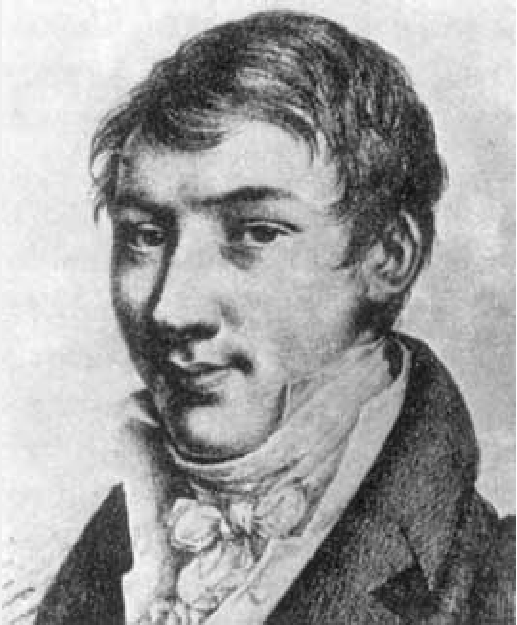
\includegraphics[width=\linewidth]{external/images/Cauchy.png}
\end{image}%
\tcblower
\end{figureptx}%
\begin{theorem}{Theorem}{Cauchy's Form of the Remainder.}{}{thm_CauchyRemainder}%
\index{Remainder of the Taylor Series!Cauchy Form of}%
\index{sequences!Cauchy sequences!Cauchy's remainder}%
Suppose \(f\) is a function such that \(f^{(n+1)}(t)\) is continuous on an interval containing \(a\) and \(x\). Then%
\begin{equation}
f(x)-\left(\sum_{j=0}^n\frac{f^{(j)}(a)}{j!}(x-a)^j\right)=\frac{f^{\, (n+1)}(c)}{n!}(x-c)^n(x-a)\label{EQUATIONCauchyFormRemainder}
\end{equation}
where \(c\) is some number between \(a\) and \(x\).%
\end{theorem}
\begin{problem}{Problem}{}{TaylorSeries-CauchyFormRem-7}%
Prove \hyperref[thm_CauchyRemainder]{Theorem~{\xreffont\ref{thm_CauchyRemainder}}} using an argument similar to the one used in the proof of \hyperref[thm_LagrangeRemainder]{Theorem~{\xreffont\ref{thm_LagrangeRemainder}}}. Don't forget there are two cases to consider.%
\end{problem}
Using Cauchy's form of the remainder, we can prove that the binomial series%
\begin{equation*}
1+\frac{1}{2}x+\frac{\frac{1}{2}\left(\frac{1}{2}-1\right)}{2!}x^2+\frac{\frac{1}{2}\left(\frac{1}{2}-1\right)\left(\frac{1}{2}-2\right)}{3!}x^3+\cdots
\end{equation*}
converges to \(\sqrt{1+x}\) for \(x\in(-1,0).\) (Strictly speaking we only need to show this for \(x\in(-1,-1/2)\). We covered the case \(x\in [-1/2,0]\) in \hyperref[prob_Taylor_Series-Binomial_Series_and]{Problem~{\xreffont\ref{prob_Taylor_Series-Binomial_Series_and}}}.)%
\par
With this in mind, let \(x\) be a fixed number with \(-1\lt x\lt 0\) and consider that the binomial series is the Maclaurin series for the function \(f(x)=(1+x)^{\frac{1}{2}}\). As we saw before,%
\begin{equation*}
f^{(n+1)}(t)=\left(\frac{1}{2}\right)\left(\frac{1}{2}-1\right)\cdots\left(\frac{1}{2}-n\right)\left(1+t\right)^{\frac{1}{2}-(n+1)}\text{,}
\end{equation*}
so the Cauchy form of the remainder is given by%
\begin{equation*}
\frac{f^{\left(n+1\right)}\left(c\right)}{n!}{\left(x-c\right)}^n\left(x-0\right)=\frac{\left(\frac{1}{2}\right)\left(\frac{1}{2}-1\right)\dots
\left(\frac{1}{2}-n\right)}{n!}\frac{{\left(x-c\right)}^n}{{\left(1+c\right)}^{n+\frac{1}{2}}}\cdot
x
\end{equation*}
where \(c\) is some number with \(x\le c\le 0\).  Thus we have%
\begin{equation*}
0\le
\left|\frac{f^{\left(n+1\right)}\left(c\right)}{n!}{\left(x-c\right)}^n\left(x-0\right)\right|=\left|\frac{\left(\frac{1}{2}\right)\left(\frac{1}{2}-1\right)\dots
\left(\frac{1}{2}-n\right)}{n!}\frac{{\left(x-c\right)}^n}{{\left(1+c\right)}^{n+\frac{1}{2}}}\cdot
x\right|
\end{equation*}
%
\par
Notice that if \(-1\lt x\leq c\),\(\) then \(0\lt 1+x\leq 1+c\). Thus \(0\lt \frac{1}{1+c}\leq\frac{1}{1+x}\) and \(\frac{1}{\sqrt{1+c}}\leq\frac{1}{\sqrt{1+x}}\). Thus we have%
\begin{equation*}
0\leq\left|\frac{\left(\frac{1}{2}\right)\left(\frac{1}{2}-1\right)\cdots\left(\frac{1}{2}-n\right)}{n!}\frac{(x-c)^nx}{(1+c)^{n+\frac{1}{2}}}\right|\leq\left(\frac{c-x}{1+c}\right)^n\frac{|\,x|}{\sqrt{1+x}}\text{.}
\end{equation*}
%
\begin{problem}{Problem}{}{TaylorSeries-CauchyFormRem-11}%
Suppose \(-1\lt x\leq c\leq 0\) and consider the function \(g(c)=\frac{c-x}{1+c}\). Show that on \([x,0]\), \(g\) is increasing and use this to conclude that for \(-1\lt x\leq c\leq 0\),%
\begin{equation*}
\frac{c-x}{1+c}\leq|x|\text{.}
\end{equation*}
%
\par
Use this fact to finish the proof that the binomial series converges to \(\sqrt{1+x}\) for \(-1\lt x\lt 0\).%
\end{problem}
\begin{problem}{Problem}{}{TaylorSeries-CauchyFormRem-12}%
Find the \hyperref[EQUATIONIntFormRemainder]{Integral form}, \hyperref[EQUATIONLagFormRemainder]{Lagrange form}, and \hyperref[EQUATIONCauchyFormRemainder]{Cauchy form} of the remainder for Taylor series of the following functions expanded about the given values of \(a\).%
\begin{enumerate}[font=\bfseries,label=(\alph*),ref=\alph*]%
\item{}\(f(x)=e^x\), \(a=0\)%
\item{}\(f(x)=\sqrt{x}\), \(a=1\)%
\item{}\(f(x)=(1+x)^\alpha\), \(a=0\)%
\item{}\(f(x)=\frac{1}{x}\), \(a=3\)%
\item{}\(f(x)=\ln x,\ a=2\)%
\item{}\(f(x)=\cos x, a=\frac{\pi}{2}\)%
\end{enumerate}%
\end{problem}
The proofs of both the \hyperref[thm_LagrangeRemainder]{Lagrange Form} and the \hyperref[thm_CauchyRemainder]{Cauchy Form} of the remainder of Taylor series made use of two crucial facts about continuous functions.  First, we assumed the \hyperref[thm_EVT]{Extreme Value Theorem}: Any continuous function on a closed bounded interval assumes its maximum and minimum somewhere on the interval.  Second, we assumed that any continuous function satisfied the \hyperref[IntermediateValueTheorem]{Intermediate Value Theorem}: If a continuous function takes on two different values, then it must take on any value between those two values.%
\par
Mathematicians in the late \(1700\)s and early \(1800\)s typically considered these facts to be intuitively obvious. This was natural since our understanding of continuity at that time was solely intuitive.  Intuition is a useful tool but as we have seen before it is also unreliable.  For example consider the following function%
\begin{align}
f(x)= 
\begin{cases}
x\sin\left(\frac{1}{x}\right),\amp \text{if } x\neq 0,\\
0, \amp \text{ if } x=0 
\end{cases} \text{.}\label{xsin1x}
\end{align}
%
\par
Is this function continuous at \(0\)?  Near zero its graph looks like this:%
\begin{figureptx}{Figure}{The graph of \(f(x)= 
\begin{cases}
x\sin\left(\frac{1}{x}\right),\amp \text{if } x\neq 0 \\
0, \amp \text{ if } x=0 
\end{cases} \) near \(0\).}{TaylorSeries-CauchyFormRem-16}{}%
\begin{image}{0.1}{0.8}{0.1}{}%
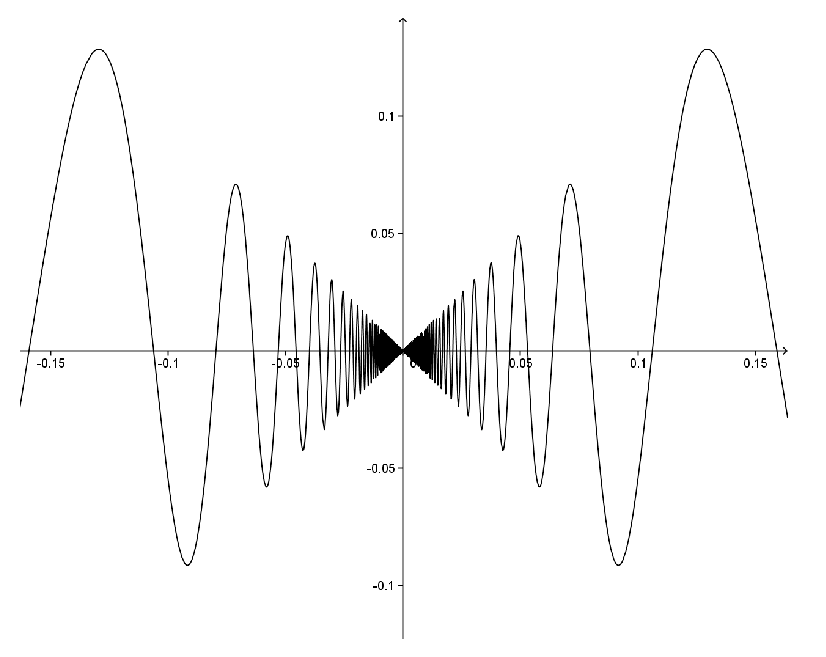
\includegraphics[width=\linewidth]{external/images/Ch5fig4.png}
\end{image}%
\tcblower
\end{figureptx}%
It is impossible to show in the sketch but this graph oscillates infinitely often as \(x\) nears zero.%
\par
No matter what your guess may be, it is clear that it is hard to analyze such a function armed with only an intuitive notion of continuity.  We will revisit this example in the next chapter.%
\par
As with convergence, continuity is more subtle than it first appears.%
\par
We put convergence on solid ground by providing a completely analytic definition in the previous chapter.  What we need to do in the next chapter is provide a completely rigorous definition for continuity.%
\end{sectionptx}
\end{chapterptx}
%
%
\typeout{************************************************}
\typeout{Chapter 8 Continuity: What It Isn't and What It Is}
\typeout{************************************************}
%
\begin{chapterptx}{Chapter}{Continuity: What It Isn't and What It Is}{}{Continuity: What It Isn't and What It Is}{}{}{Continuity}
\renewcommand*{\chaptername}{Chapter}
%
%
\typeout{************************************************}
\typeout{Section 8.1 An Analytic Definition of Continuity}
\typeout{************************************************}
%
\begin{sectionptx}{Section}{An Analytic Definition of Continuity}{}{An Analytic Definition of Continuity}{}{}{Continuity-AnalyticDef}
Before the invention of Calculus, the notion of continuity was treated intuitively if it was treated at all. This was reasonable because at first pass it seems to be a very simple idea based solidly in our experience of the real world. Standing on the bank we see a river flow past us continuously, not by tiny jerks.  Even when the flow might seem at first to be discontinuous, as when it drops precipitously over a cliff, a closer examination shows that it really is not.  As the water approaches the cliff it speeds up.  When it finally goes over it accelerates very quickly but no matter how fast it goes it moves continuously, moving from here to there by occupying every point in between.  This is continuous motion.  It never disappears over there and instantaneously reappears over here.  That would be discontinuous motion.%
\par
Similarly, a thrown stone flies continuously (and smoothly) from release point to landing point, passing through each point in its path.%
\par
But wait.%
\par
If the stone passes through discrete points it must be doing so by teeny tiny little jerks, mustn't it?  Otherwise how would it get from one point to the next?  Is it possible that motion in the real world, much like motion in a movie, is really composed of tiny jerks from one point to the next but that these tiny jerks are simply too small and too fast for our senses to detect?%
\par
If so, then the real world is more like the rational number line (\(\QQ\)) from \hyperref[NumbersRealRational]{Chapter~{\xreffont\ref{NumbersRealRational}}} than the real number line (\(\RR\)).  In that case, motion really consists of jumping discretely over the missing points (like \(\sqrt{2}\)) as we move from here to there. That may seem like a bizarre idea to you \textemdash{} it does to us as well \textemdash{} but the idea of continuous motion is equally bizarre.  It's just a little harder to see why since it is so familiar.%
\par
The real world will be what it is regardless of what we believe it to be, but fortunately in mathematics we are not constrained to live in it.  So we won't even try.  We will simply postulate that no such jerkiness exists; that all motion is continuous.%
\par
However we are constrained to live with the logical consequences of our assumptions, once they are made.  These will lead us into some very deep waters indeed.%
\par
The intuitive treatment of continuity was maintained throughout the 1700's as it was not generally perceived that a truly rigorous definition was necessary.  Consider the following definition given by Euler in 1748.%
\begin{quote}%
A continuous curve is one such that its nature can be expressed by a single function of \(x.\) If a curve is of such a nature that for its various parts . . . different functions of \(x\) are required for its expression, . . . , then we call such a curve discontinuous.%
\end{quote}
However, the complexities associated with Fourier series and the types of functions that they represented caused mathematicians in the early \(1800\)s to rethink their notions of continuity.  As we saw in \hyperref[InterregnumPart]{Part~{\xreffont\ref{InterregnumPart}}}, the graph of the function defined by the Fourier series%
\begin{equation*}
\frac{4}{\pi}\sum_{k=0}^\infty\frac{\left(-1\right)^k}{\left(2k+1\right)} \cos \left(\left(2k+1\right)\pi x\right)
\end{equation*}
looked like this:%
\begin{figureptx}{Figure}{Graph of \(\frac{4}{\pi}\sum_{k=0}^\infty\frac{\left(-1\right)^k}{\left(2k+1\right)} \cos \left(\left(2k+1\right)\pi x\right)\)}{Continuity-AnalyticDef-12}{}%
\begin{image}{0.125}{0.75}{0.125}{}%
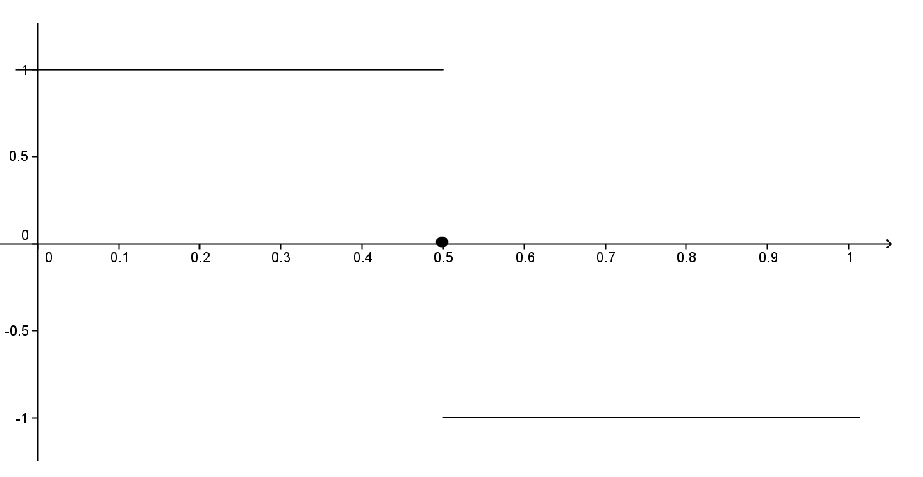
\includegraphics[width=\linewidth]{external/images/Ch5fig1.png}
\end{image}%
\tcblower
\end{figureptx}%
This function went against Euler's notion of what continuous functions should be.  Here, an infinite sum of continuous cosine curves provided a single expression which resulted in a ``discontinuous'' curve.  But as we've seen this didn't happen with power series and an intuitive notion of continuity is inadequate to explain the difference.  Even more perplexing is the following situation.  Intuitively, one would think that a continuous curve should have a tangent line at at least one point.  It may have a number of jagged points to it, but it should be ``smooth'' somewhere.  An example of this would be \(f(x)=x^{2/3}\).  Its graph is given by%
\begin{figureptx}{Figure}{Graph of \(f(x)=x^{2/3}\).}{Continuity-AnalyticDef-14}{}%
\begin{image}{0.125}{0.75}{0.125}{}%
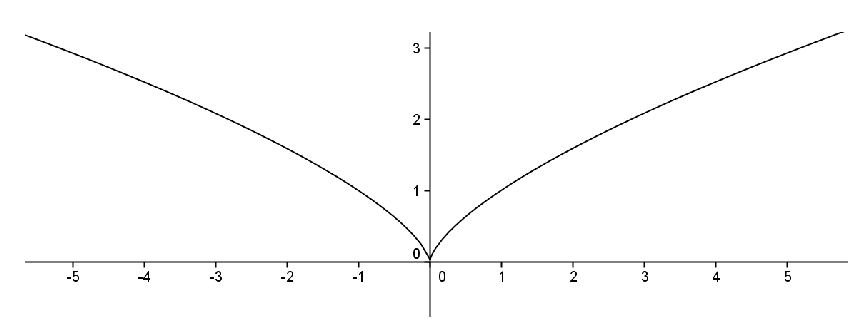
\includegraphics[width=\linewidth]{external/images/Ch5fig2.png}
\end{image}%
\tcblower
\end{figureptx}%
This function is not differentiable at the origin but it is differentiable everywhere else.  One could certainly come up with examples of functions which fail to be differentiable at any number of points but, intuitively, it would be reasonable to expect that a continuous function should be differentiable \emph{somewhere}.  We might conjecture the following:%
\begin{conjecture}{Conjecture}{}{}{conj_ContImplyDiff}%
If \(f\) is continuous on an interval \(I\) then there is some \(a\in I\), such that \(f^\prime(a)\) exists.%
\end{conjecture}
\index{Weierstrass, Karl} Surprisingly, in \(1872\), \href{https://mathshistory.st-andrews.ac.uk/Biographies/Weierstrass/}{Karl Weierstrass} (1815\textendash{}1897) showed that the above conjecture is \alert{FALSE}. He did this by displaying the counterexample:%
\begin{equation*}
f(x)=\sum_{n=0}^\infty b^n\cos(a^n\pi x)\text{.}
\end{equation*}
%
\begin{figureptx}{Figure}{Karl Weierstrass}{Continuity-AnalyticDef-18}{}%
\index{Weierstrass, Karl!portrait of}%
\index{Portraits!Weierstrass}%
\begin{image}{0.325}{0.35}{0.325}{}%
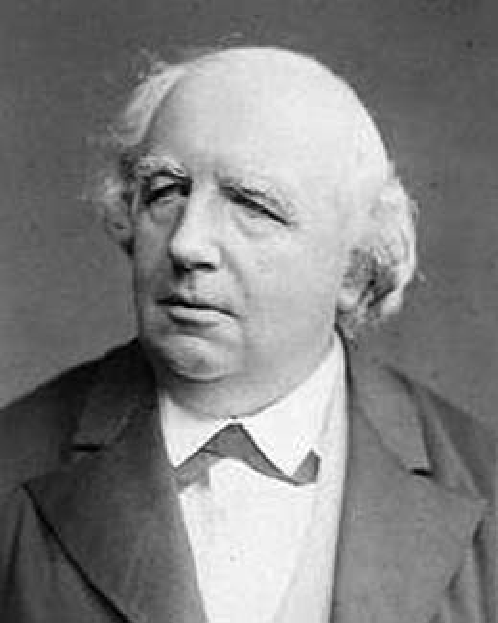
\includegraphics[width=\linewidth]{external/images/Weierstrass.png}
\end{image}%
\tcblower
\end{figureptx}%
Weierstrass showed that if \(a\) is an odd integer, \(b\in(0,1)\), and \(ab>1+\frac{3}{2}\pi\), then \(f\) is continuous everywhere, but is nowhere differentiable.  Such a function is somewhat ``fractal'' in nature, and it is clear that a definition of continuity relying on intuition is inadequate to study it.%
\begin{problem}{Problem}{}{Continuity-AnalyticDef-20}%
\begin{enumerate}[font=\bfseries,label=(\alph*),ref=\alph*]%
\item{}Given \(f(x)=\sum_{n=0}^\infty\left(\frac{1}{2}\right)^n\cos\left(a^n\pi
x\right)\), what is the smallest value of \(a\) for which \(f\) satisfies Weierstrass' criterion to be continuous and nowhere differentiable.%
\item{}Let \(f(x,N)=\sum_{n=0}^N\left(\frac{1}{2}\right)^n\cos\left(13^n\pi
x\right)\) and use a computer algebra system to plot \(f(x,N)\) for \(N=0,1,2,3,4,10\) and \(x\in[0,1]\).%
\item{}Plot \(f(x,10)\) for \(x\in[\,0,c]\), where \(c=0.1,0.01,0.001,0.0001,0.00001\).  Based upon what you see in parts b and c, why would we describe the function to be somewhat ``fractal'' in nature?%
\end{enumerate}%
\end{problem}
Just as it was important to define convergence with a rigorous definition without appealing to intuition or geometric representations, it is imperative that we define continuity in a rigorous fashion not relying on graphs.%
\par
\index{Bolzano, Bernhard} The first definition of continuity which did not rely on geometry or intuition was given in 1817 by \href{https://mathshistory.st-andrews.ac.uk/Biographies/Bolzano/}{Bernhard Bolzano} (1781\textendash{}1848) in a paper published in the Proceedings of the Prague Scientific Society entitled \textit{Rein analytischer Beweis des Lehrsatzes dass zwieschen je zwey Werthen, die ein entgegengesetztes Resultat gewaehren, wenigstens eine reele Wurzel der Gleichung liege} (Purely Analytic Proof of the Theorem that Between Any Two Values that Yield Results of Opposite Sign There Will be at Least One Real Root of the Equation).%
\begin{figureptx}{Figure}{Bernhard Bolzano}{Continuity-AnalyticDef-23}{}%
\index{Bolzano, Bernhard!portrait of}%
\index{Portraits!Bolzano}%
\begin{image}{0.325}{0.35}{0.325}{}%
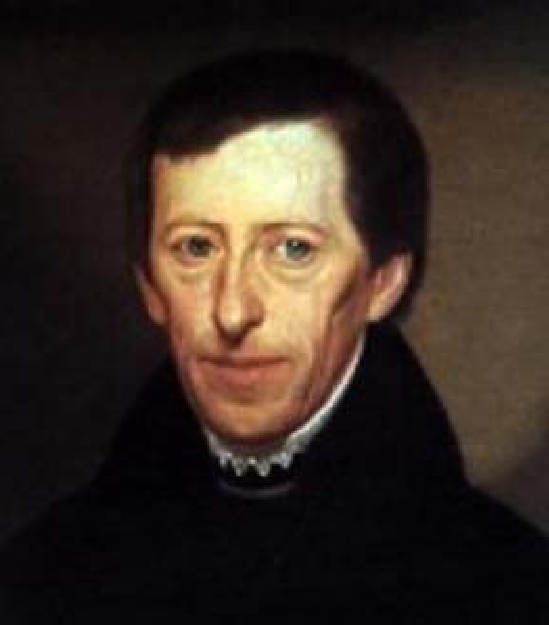
\includegraphics[width=\linewidth]{external/images/Bolzano.png}
\end{image}%
\tcblower
\end{figureptx}%
From the title it should be clear that in this paper Bolzano is proving the \hyperref[IntermediateValueTheorem]{Intermediate Value Theorem}.  To do this he needs a completely analytic definition of continuity.  The substance of Bolzano's idea is that if \(f\) is continuous at a point \(a\) then \(f(x)\) should be ``close to'' \(f(a)\) whenever \(x\) is ``close enough to'' \(a\).  More precisely, Bolzano said that \(f\) is continuous at \(a\) provided \(\abs{f(x)-f(a)}\) can be made smaller than any given quantity provided we make \(\abs{x-a}\) sufficiently small.%
\par
\index{Leibniz, Gottfried Wilhelm} The language Bolzano uses is very similar to the language Leibniz used when he postulated the existence of infinitesimally small numbers.  Leibniz said that infinitesimals are ``smaller than any given quantity but not zero.'' Bolzano says that ``\(\abs{f(x)-f(a)}\) can be made smaller than any given quantity provided we make \(\abs{x-a}\) sufficiently small.'' But Bolzano stops short of saying that \(\abs{x-a}\) is infinitesimally small. He says that given \(a\), we can choose \(x\) so that \(\abs{x-a}\) is smaller than any real number we could name, say \(b\), provided we name \(b\) first. But for any given choice of \(x\), \(\abs{x-a}\), and \(b\) are both still real numbers.  Possibly very small real numbers to be sure, but real numbers nonetheless.  Infinitesimals have no place in Bolzano's construction.%
\par
\index{Bolzano, Bernhard}\index{Cauchy, Augustin} Bolzano's paper was not well known when Cauchy proposed a similar definition in his \emph{Cours d'analyse}~\hyperlink{bradley09__cauch_cours}{[{\xreffont 1}]} of 1821 so it is usually Cauchy who is credited with this definition, but even Cauchy's definition is not quite tight enough for modern standards.  It was Karl Weierstrass in 1859 who finally gave the modern definition.%
\begin{definition}{Definition}{Continuity at a Point.}{def_continuity}%
\index{continuity!at a point}%
\index{Definition!continuity!at a point}%
We say that a function \(f\) is continuous at the point \(a\) provided that for each \(\eps\gt0\), there exists a \(\delta\gt0\) such that if \(\abs{x-a}\lt \delta\) then \(|f(x)-f(a)|\lt \eps\).%
\end{definition}
\index{continuity!on an interval} Notice that the definition of continuity of a function is done point\textendash{}by\textendash{}point so a function can certainly be continuous at some points while discontinuous at others.  When we say that \(f\) is \terminology{continuous on an interval}, then we mean that it is continuous at every point of that interval and, in theory, we would need to use the above definition to check continuity at each individual point.%
\par
\index{Extreme Value Theorem (EVT)!continuity and}\index{continuity!Extreme Value Theorem (EVT) and}\index{Intermediate Value Theorem (IVT)!continuity and}\index{continuity!Intermediate Value Theorem and} Our definition fits the bill in that it does not rely on either intuition or graphs, but it is this very non-intuitiveness that makes it hard to grasp.  It usually takes some time to become comfortable with this definition, let alone use it to prove theorems such as the \hyperref[thm_EVT]{Extreme Value Theorem} and \hyperref[IntermediateValueTheorem]{Intermediate Value Theorem}.  So let's go slowly to develop a feel for it.%
\par
This definition spells out a completely black and white procedure: you give me a positive number \(\eps\), and I must be able to find a positive number \(\delta\) which satisfies a certain property.  If I can always do that then the function is continuous at the point of interest.%
\par
This definition also makes very precise what we mean when we say that \(f(x)\) should be ``close to'' \(f(a)\) whenever \(x\) is ``close enough to'' \(a\).  For example, intuitively we know that \(f(x)=x^2\) should be continuous at \(x=2\).  This means that we should be able to get \(x^2\) to within, say, \(\eps=0.1\) of \(4\) provided we make \(x\) close enough to \(2\).  Specifically, we want \(3.9\lt x^2\lt 4.1\).  This happens exactly when \(\sqrt{3.9}\lt x\lt \sqrt{4.1}\).  Using the fact that \(\sqrt{3.9}\lt 1.98\) and \(2.02\lt \sqrt{4.1}\), then we can see that if we get \(x\) to within \(\delta=.02\) of \(2\), then \(\sqrt{3.9}\lt 1.98\lt x\lt 2.02\lt
\sqrt{4.1}\) and so \(x^2\) will be within .\(1\) of \(\,4\).  This is very straightforward.  What makes this situation more difficult is that we must be able to do this for any \(\eps>0\).%
\par
Notice the similarity between this definition and the definition of convergence of a sequence.  Both definitions have the challenge of an \(\eps>0\).  In the definition of \(\limit{n}{\infty}{s_n}=s\), we had to get \(s_n\) to within \(\eps\) of \(s\) by making \(n\) large enough.  For sequences, the challenge lies in making \(\abs{s_n-s}\) sufficiently small.  More precisely, given \(\eps>0\) we need to decide how large \(n\) should be to guarantee that \(\abs{s_n-s}\lt \eps\).%
\par
In our definition of continuity, we still need to make something small (namely \(\abs{f(x)-f(a)}\lt \eps\)), only this time, we need to determine how close \(x\) must be to \(a\) to ensure this will happen instead of determining how large \(n\) must be.%
\par
What makes \(f\) continuous at \(a\) is the arbitrary nature of \(\eps\) (as long as it is positive).  As \(\eps\) becomes smaller, this forces \(f(x)\) to be closer to \(f(a)\).  That we can always find a positive distance \(\delta\) to work is what we mean when we say that we can make \(f(x)\) as close to \(f(a)\) as we wish, provided we get \(x\) close enough to \(a\).  The sequence of pictures below illustrates that the phrase ``for any \(\eps>0\), there exists a \(\delta>0\) such that if \(|\,x-a|\lt \delta\) then \(|f(x)-f(a)|\lt \eps\)'' can be replaced by the equivalent formulation ``for any \(\eps>0\), there exists a \(\delta>0\) such that if \(a-\delta\lt x\lt a+\delta\) then \(f(a)-\eps\lt f(x)\lt
f(a)+\eps\).'' This could also be replaced by the phrase ``for any \(\eps>0\), there exists a \(\delta>0\) such that if \(x\in(a-\delta,a+\delta)\) then \(f(x)\in(f(a)-\eps,f(a)+\eps)\).'' All of these equivalent formulations convey the idea that we can get \(f(x)\) to within \(\eps\) of \(f(a)\), provided we make \(x\) within \(\delta\) of \(a\), and we will use whichever formulation suits our needs in a particular application.%
\begin{sidebyside}{2}{0.025}{0.025}{0.05}%
\begin{sbspanel}{0.45}[center]%
\noindent\includegraphics[width=\linewidth]{external/images/Ch5fig3a.png}
\end{sbspanel}%
\begin{sbspanel}{0.45}[center]%
\noindent\includegraphics[width=\linewidth]{external/images/Ch5fig3b.png}
\end{sbspanel}%
\end{sidebyside}%
\begin{sidebyside}{2}{0.025}{0.025}{0.05}%
\begin{sbspanel}{0.45}[center]%
\noindent\includegraphics[width=\linewidth]{external/images/Ch5fig3c.png}
\end{sbspanel}%
\begin{sbspanel}{0.45}[center]%
\noindent\includegraphics[width=\linewidth]{external/images/Ch5fig3d.png}
\end{sbspanel}%
\end{sidebyside}%
The precision of the definition is what allows us to examine continuity without relying on pictures or vague notions such as ``nearness'' or ``getting closer to.'' We will now consider some examples to illustrate this precision.%
\begin{example}{Example}{}{Continuity-AnalyticDef-37}%
Use the definition of continuity to show that \(f(x)=x\) is continuous at any point \(a\).%
\end{example}
If we were to draw the graph of this function, then you would likely say that this is obvious.  The point behind the definition is that we can back up your intuition in a rigorous manner.%
\begin{proof}{Proof}{}{Continuity-AnalyticDef-39}
Let \(\eps>0\). Let \(\delta=\eps\). If \(|\,x-a|\lt \delta\), then%
\begin{equation*}
|f(x)-f(a)|=|\,x-a|\lt \eps
\end{equation*}
%
\begin{aside}{Aside}{Choosing \(\delta{}\).}{Continuity-AnalyticDef-39-2}%
Take particular note in these proofs that our choice of \(\delta\) guarantees that \(\delta\gt0\). This is obvious now. But as things become more complicated \textemdash{} for example, see \hyperref[prob_Cauchy_s_incorrect_proof]{Problem~{\xreffont\ref{prob_Cauchy_s_incorrect_proof}}} \textemdash{} it will be easy to chose a \(\delta\) that could be equal to zero which will invalidate the proof.%
\par
Also, the goal is to write clearly and concisely, but it is better to be clear and a little verbose than to be so concise that your meaning is hidden. So when writing proofs this delicate it is important to take great care to be very clear.  If there is any possible ambiguity it is better to state explicitly that, for example, ``\(\delta \gt
0\)'', rather than leaving it to the reader to figure out.%
\end{aside}
Thus by the definition, \(f\) is continuous at \(a\).%
\end{proof}
\begin{problem}{Problem}{}{Continuity-AnalyticDef-40}%
Use the definition of continuity to show that if \(m\) and \(b\) are fixed (but unspecified) real numbers then the function%
\begin{equation*}
f(x) = mx+b
\end{equation*}
is continuous at every real number \(a\).%
\end{problem}
\begin{example}{Example}{}{Continuity-AnalyticDef-41}%
Use the definition of continuity to show that \(f(x)=x^2\) is continuous at \(a=0\).%
\end{example}
\begin{proof}{Proof}{}{Continuity-AnalyticDef-42}
Let \(\eps>0\). Let \(\delta=\sqrt{\eps}\). If \(|\,x-0|\lt \delta\), then \(|\,x|\lt \sqrt{\eps}\). Thus%
\begin{equation*}
\abs{x^2-0^2}=|\,x|^2\lt \left(\sqrt{\eps}\right)^2=\eps\text{.}
\end{equation*}
%
\par
Thus by the definition, \(f\) is continuous at \(0\).%
\end{proof}
Notice that in these proofs, the challenge of an \(\eps>0\) was given first.  This is because the choice of \(\delta\) must depend upon \(\eps\).  Also notice that there was no explanation for our choice of \(\delta\).  We just supplied it and showed that it worked.  As long as \(\delta>0\), then this is all that is required.  In point of fact, the \(\delta\) we chose in each example was not the only choice that worked; any smaller \(\delta\) would work as well.%
\begin{problem}{Problem}{}{Continuity-AnalyticDef-44}%
\begin{enumerate}[font=\bfseries,label=(\alph*),ref=\alph*]%
\item{}Given a particular \(\eps>0\) in the definition of continuity, show that if a particular \(\delta_0>0\) satisfies the definition, then any \(\delta\) with \(0\lt \delta\lt \delta_0\) will also work for this \(\eps\).%
\item{}Show that if a \(\delta\) can be found to satisfy the conditions of the definition of continuity for a particular \(\eps_0>0\), then this \(\delta\) will also work for any \(\,\eps\) with \(0\lt \eps_0\lt
\eps\).%
\end{enumerate}%
\end{problem}
It wasn't explicitly stated in the definition but when we say ``if \(\abs{x-a}\lt \delta\) then \(|f(x)-f(a)|\lt
\eps\),'' we should be restricting ourselves to \(x\) values which are in the domain of the function \(f\), otherwise \(f(x)\) doesn't make sense.  We didn't put it in the definition because that definition was complicated enough without this technicality.  Also in the above examples, the functions were defined everywhere so it was a moot point.  We will continue with the convention that when we say ``if \(|\,x-a|\lt \delta\) then \(|f(x)-f(a)|\lt \eps\),'' we will be restricting ourselves to \(x\) values which are in the domain of the function \(f\).  This will allow us to examine continuity of functions not defined for all \(x\) without restating this restriction each time.%
\begin{problem}{Problem}{}{prob_extended_sqrt_is_continuous_at_zero}%
\index{continuity!\(\pm\sqrt{x}\) is continuous at zero} Use the definition of continuity to show that%
\begin{equation*}
f(x)= \begin{cases}\sqrt{x} \amp  \text{ if }  x\ge0\\ -\sqrt{-x} \amp  \text{ if }  x\lt 0 \end{cases}
\end{equation*}
is continuous at \(a=0\).%
\end{problem}
\begin{problem}{Problem}{}{Continuity-AnalyticDef-47}%
Use the definition of continuity to show that \(f(x)=
\sqrt{x}\) is continuous at \(a=0\).  How is this problem different from \hyperref[prob_extended_sqrt_is_continuous_at_zero]{Problem~{\xreffont\ref{prob_extended_sqrt_is_continuous_at_zero}}}?  How is it similar?%
\end{problem}
Sometimes the \(\delta\) that will work for a particular \(\eps\) is fairly obvious to see, especially after you've gained some experience.  This is the case in the above examples (at least after looking back at the proofs).  However, finding \(\delta\) is usually not so obvious and requires some scrapwork.  This scrapwork is vital toward producing a \(\delta\), but again is not part of the polished proof. This can be seen in the following example.%
\begin{example}{Example}{}{example_SqrtContinuous}%
Use the definition of continuity to prove that \(f(x)=\sqrt{x}\) is continuous at \(a=1\).%
\par
\terminology{SCRAPWORK}%
\par
As before, the scrapwork for these problems often consists of simply working backwards.  Specifically, given an \(\eps>0\), we need to find a \(\delta>0\) so that \(\abs{\sqrt{x}-\sqrt{1}}\lt \eps\), whenever \(\abs{x-1}\lt
\delta\).  We work backwards from what we want, keeping an eye on the fact that we can control the size of \(\abs{x-1}\).%
\begin{equation*}
\abs{\sqrt{x}-\sqrt{1}}=\abs{\frac{\left(\sqrt{x}-1\right)\left(\sqrt{x}+1\right)}{\sqrt{x}+1}|}=\frac{\abs{x-1}}{\sqrt{x}+1}\lt
\abs{x-1}\text{.}
\end{equation*}
%
\par
This seems to suggest that we should make \(\delta=\eps\). We're now ready for the formal proof.%
\end{example}
\begin{proof}{Proof}{}{Continuity-AnalyticDef-50}
Let \(\eps>0\). Let \(\delta=\eps\). If \(\abs{x-1}\lt \delta\), then \(\abs{x-1}\lt \eps\), and so%
\begin{equation*}
\abs{\sqrt{x}-\sqrt{1}}=\abs{\frac{\left(\sqrt{x}-1\right)\left(\sqrt{x}+1\right)}{ \sqrt{x}+1}}=\frac{\abs{x-1}}{\sqrt{x}+1}\lt \abs{x-1}\lt \eps\text{.}
\end{equation*}
%
\par
Thus by definition, \(f(x)=\sqrt{x}\) is continuous at \(1\).%
\end{proof}
Bear in mind that someone reading the formal proof will not have seen the scrapwork, so the choice of \(\delta\) might seem rather mysterious.  However, you are in no way bound to motivate this choice of \(\delta\) and usually you should not, unless it is necessary for the formal proof.  All you have to do is find this \(\delta\) and show that it works.   To a trained reader, your ideas will come through when you demonstrate that your choice of \(\delta\) works.%
\begin{figureptx}{Figure}{\href{https://mathshistory.st-andrews.ac.uk/Biographies/Halmos/}{Paul Halmos}}{Continuity-AnalyticDef-52}{}%
\index{Halmos, Paul!portrait of}%
\index{Portraits!Halmos}%
\begin{image}{0.325}{0.35}{0.325}{}%
\includegraphics[width=\linewidth]{external/images/Halmos.png}
\end{image}%
\tcblower
\end{figureptx}%
\index{Halmos, Paul} Now reverse this last statement.  \emph{As} a trained reader, when you read the proof of a theorem it is \emph{your} responsibility to find the scrapwork, to see how the proof works and understand it fully.  As the renowned mathematical expositor Paul Halmos  (1916-2006) said,%
\begin{quote}%
``Don't just read it; fight it! Ask your own questions, look for your own examples, discover your own proofs. Is the hypothesis necessary? Is the converse true? What happens in the classical special case? What about the degenerate cases? Where does the proof use the hypothesis?''%
\end{quote}
This is the way to learn mathematics.  It is really the only way.%
\begin{problem}{Problem}{}{Continuity-AnalyticDef-56}%
Use the definition of continuity to show that \(f(x)=\sqrt{x}\) is continuous at any positive real number \(a\).%
\end{problem}
\begin{problem}{Problem}{}{Continuity-AnalyticDef-57}%
\begin{enumerate}[font=\bfseries,label=(\alph*),ref=\alph*]%
\item{}Use a unit circle to show that for \(0\leq\theta\lt
\frac{\pi}{2}\), \(\sin \theta\leq\theta\) and \(1-\cos \theta\leq\theta\) and conclude \(\abs{\sin
\theta}\leq\abs{\theta}\) and \(\abs{1-\cos
\theta}\leq\abs{\theta}\) for \(-\frac{\pi}{2}\lt
\theta\) \(\lt \frac{\pi}{2}\).%
\item{}Use the definition of continuity to prove that \(f(x)=\sin x\) is continuous at any point \(a\).%
\par\smallskip%
\noindent\textbf{\blocktitlefont Hint}.\hypertarget{Continuity-AnalyticDef-57-3-2}{}\quad{}\(\sin x=\sin\left(x-a+a\right)\).%
\end{enumerate}%
\end{problem}
\begin{problem}{Problem}{}{Continuity-AnalyticDef-58}%
\begin{enumerate}[font=\bfseries,label=(\alph*),ref=\alph*]%
\item{}Use the definition of continuity to show that \(f(x)=e^x\) is continuous at \(a=0\).%
\item{}Show that \(f(x)=e^x\) is continuous at any point \(a\).%
\par\smallskip%
\noindent\textbf{\blocktitlefont Hint}.\hypertarget{Continuity-AnalyticDef-58-4-2}{}\quad{}Rewrite \(e^x-e^a\) as \(e^{a+(x-a)}-e^a\) and use what you proved in part a.%
\end{enumerate}%
\end{problem}
In the above problems, we used the definition of continuity to verify our intuition about the continuity of familiar functions.  The advantage of this analytic definition is that it can be applied when the function is not so intuitive.  Consider, for example, the function given at the end of the last chapter.%
\begin{equation*}
f(x)= \begin{cases}
x\,\sin\left(\frac{1}{x}\right),\amp \text{ if } x\neq 0\\
0, \amp \text{ if } x=0 
\end{cases}  \text{.}
\end{equation*}
%
\par
Near zero, the graph of \(f(x)\) looks like this:%
\begin{image}{0.125}{0.75}{0.125}{}%
\includegraphics[width=\linewidth]{external/images/Ch5fig4.png}
\end{image}%
As we mentioned in the previous chapter, since sin\(\left(\frac{1}{x}\right)\) oscillates infinitely often as \(x\) nears zero this graph must be viewed with a certain amount of suspicion.  However our completely analytic definition of continuity shows that this function is, in fact, continuous at 0.%
\begin{problem}{Problem}{}{Continuity-AnalyticDef-63}%
Use the definition of continuity to show that%
\begin{equation*}
f(x)= \begin{cases}
x\,\sin\left(\frac{1}{x}\right),\amp \text{ if } x\neq 0\\ 
0, \amp \text{ if } x=0 
\end{cases}
\end{equation*}
is continuous at \(0\).%
\end{problem}
Even more perplexing is the function defined by%
\begin{equation*}
D(x)=
\left\{ 
\begin{matrix}
x\text{,} \amp \text{ if } x\text{ is rational } \\
0\text{,} \amp \text{ if } x\text{ is irrational. } 
\end{matrix}
\right.
\end{equation*}
     %
\par
To the naked eye, the graph of this function looks like the lines \(y=0\) and \(y=x\).  Of course, such a graph would not be the graph of a function.  Actually, both of these lines have holes in them.  Wherever there is a point on one line there is a ``hole'' on the other.  Each of these holes is the width of a single point (that is, their ``width'' is zero!) so they are invisible to the naked eye (or even magnified under the most powerful microscope available).  This idea is illustrated in the following graph%
\begin{image}{0.2}{0.6}{0.2}{}%
\includegraphics[width=\linewidth]{external/images/Ch5fig5.png}
\end{image}%
Can such a function so ``full of holes'' actually be continuous anywhere?  It turns out that we can use our definition to show that this function is, in fact, continuous at \(0\) and at no other point.%
\begin{problem}{Problem}{}{Continuity-AnalyticDef-68}%
\begin{enumerate}[font=\bfseries,label=(\alph*),ref=\alph*]%
\item{}Use the definition of continuity to show that the function%
\begin{equation*}
D(x)= \begin{cases}
x,\amp \text{ if } x\text{ is rational } \\
0,\amp \text{ if } x\text{ is irrational } \end{cases} 
\end{equation*}
is continuous at \(0\).%
\item{}Let \(a\neq 0\).  Use the definition of continuity to show that \(D\) is not continuous at \(a\).%
\par\smallskip%
\noindent\textbf{\blocktitlefont Hint}.\hypertarget{Continuity-AnalyticDef-68-3-2}{}\quad{}You might want to break this up into the two cases where \(a\) is rational or irrational.  Show that no choice of \(\delta>0\) will work for \(\eps=\abs{a}\).  Note that \hyperref[thm_IrrationalBetweenIrrationals]{Theorem~{\xreffont\ref{thm_IrrationalBetweenIrrationals}}} of \hyperref[NumbersRealRational]{Chapter~{\xreffont\ref{NumbersRealRational}}} will probably help here.%
\end{enumerate}%
\end{problem}
\begin{problem}{Problem}{}{Continuity-AnalyticDef-69}%
Use the definition of continuity to prove that the constant function \(g(x)=c\) is continuous at any point \(a\).%
\end{problem}
\begin{problem}{Problem}{}{Continuity-AnalyticDef-70}%
\begin{enumerate}[font=\bfseries,label=(\alph*),ref=\alph*]%
\item{}Use the definition of continuity to prove that \(\ln x\) is continuous at \(x1\).%
\par\smallskip%
\noindent\textbf{\blocktitlefont Hint}.\hypertarget{Continuity-AnalyticDef-70-3-2}{}\quad{}You may want to use the fact \(\abs{\ln x}\lt
\eps\,\Leftrightarrow-\eps\lt \ln x\lt \eps\) to find a \(\delta\).%
\item{}Use part (a) to prove that \(\ln x\) is continuous at any positive real number \(a\).%
\par\smallskip%
\noindent\textbf{\blocktitlefont Hint}.\hypertarget{Continuity-AnalyticDef-70-4-2}{}\quad{}\(\ln(x)=\ln(x/a)+\ln(a)\).  This is a combination of functions which are continuous at \(a\).  Be sure to explain how you know that \(\ln(x/a)\) is continuous at \(a\).%
\end{enumerate}%
\end{problem}
\begin{problem}{Problem}{}{Continuity-AnalyticDef-71}%
\index{continuity!formal definition of discontinuity} Write a formal definition of the statement \(f\) is not continuous at \(a\), and use it to prove that the function%
\begin{equation*}
f(x)= 
\begin{cases}
x\amp \text{ if } x\neq 1\\
0\amp \text{if } x=1 
\end{cases}
\end{equation*}
is not continuous at \(a=1\).%
\end{problem}
\end{sectionptx}
%
%
\typeout{************************************************}
\typeout{Section 8.2 Sequences and Continuity}
\typeout{************************************************}
%
\begin{sectionptx}{Section}{Sequences and Continuity}{}{Sequences and Continuity}{}{}{SequencesAndContinuity}
There is an alternative way to prove that the function%
\begin{equation*}
D(x)=\left\{ \begin{matrix}x\text{,} \amp \text{ if } x\text{ is rational } \\ 0\text{,} \amp \text{ if } x\text{ is irrational } \end{matrix} \right.
\end{equation*}
is not continuous at \(a\neq 0\).  We will examine this by looking at the relationship between our definitions of convergence and continuity.  The two ideas are actually quite closely connected, as illustrated by the following very useful theorem.%
\begin{theorem}{Theorem}{}{}{thm_LimDefOfContinuity}%
\index{continuity!and sequences}%
The function \(f\) is continuous at \(a\) if and only if \(f\) satisfies the following property:%
\begin{equation*}
\forall\text{ sequences } \left(x_n\right)\text{,  if }
\,\,\limit{n}{\infty}{x_n}=a \text{ then} \limit{n}{\infty}{f(x_n)}=f(a).
\end{equation*}
%
\end{theorem}
\hyperref[thm_LimDefOfContinuity]{Theorem~{\xreffont\ref{thm_LimDefOfContinuity}}} says that in order for \(f\) to be continuous, it is necessary and sufficient that any sequence \(\left(x_n\right)\) converging to \(a\) must force the sequence \(\left(f(x_n)\right)\) to converge to \(f(a)\).  A picture of this situation is below though, as always, the formal proof will not rely on the diagram.%
\begin{image}{0.315}{0.37}{0.315}{}%
\includegraphics[width=\linewidth]{external/images/Ch5fig6.png}
\end{image}%
This theorem is especially useful for showing that a function \(f,\) is not continuous at a point \(a\). All we need to do is exhibit a sequence \(\left(x_n\right)\) converging to \(a\) such that the sequence \(\limit{n}{\infty}{f(x_n)}\) does \emph{not} converge to \(f(a)\).  Let's demonstrate this idea before we tackle the proof of \hyperref[thm_LimDefOfContinuity]{Theorem~{\xreffont\ref{thm_LimDefOfContinuity}}}.%
\begin{example}{Example}{}{example_HeavisideNotContinuous}%
Use \hyperref[thm_LimDefOfContinuity]{Theorem~{\xreffont\ref{thm_LimDefOfContinuity}}} to prove that%
\begin{equation*}
f(x)= \begin{cases}\frac{|x|}{x}\text{,} \amp \text{ if } x\neq 0\\ 0\text{,} \amp \text{ if } x=0 \end{cases}
\end{equation*}
is not continuous at \(0\).%
\end{example}
\begin{proof}{Proof}{}{SequencesAndContinuity-8}
First notice that \(f\) can be written as%
\begin{equation*}
f(x)= \begin{cases}1\amp \text{ if } x>0\\ -1\amp \text{ if } x\lt 0\\ 0\amp \text{ if } x=0 \end{cases} \text{.}
\end{equation*}
%
\par
To show that \(f\) is not continuous at \(0\), all we need to do is create a single sequence \(\left(x_n\right)\) which converges to \(0\), but for which the sequence \(\left(f\left(x_n\right)\right)\) does not converge to \(f(0)=0\).  For a function like this one, just about any sequence will do, but let's use \(\left(\frac{1}{n}\right)\), just because it is an old familiar friend.%
\par
We have \(\limit{n}{\infty}{\frac{1}{n}}=0\), but \(\limit{n}{\infty}{f\left(\frac{1}{n}\right)}=\limit{n}{
\infty}{1}=1\neq 0=f(0)\).  Thus by \hyperref[thm_LimDefOfContinuity]{Theorem~{\xreffont\ref{thm_LimDefOfContinuity}}}, \(f\) is not continuous at \(0\).%
\end{proof}
\begin{problem}{Problem}{}{SequencesAndContinuity-9}%
Use \hyperref[thm_LimDefOfContinuity]{Theorem~{\xreffont\ref{thm_LimDefOfContinuity}}} to show that%
\begin{equation*}
f(x)= \begin{cases}
\frac{\abs{x}}{x},\amp \text{ if } x\neq 0\\
a, \amp \text{ if } x=0 \end{cases}  
\end{equation*}
is not continuous at \(0\), no matter what value \(a\) is.%
\end{problem}
\begin{problem}{Problem}{}{SequencesAndContinuity-10}%
Use \hyperref[thm_LimDefOfContinuity]{Theorem~{\xreffont\ref{thm_LimDefOfContinuity}}} to show that%
\begin{equation*}
D(x)= \begin{cases}
x, \amp \text{ if } x\text{ is rational } \\
0, \amp \text{ if } x\text{ is irrational } \end{cases}  
\end{equation*}
is  continuous at \(a= 0\).%
\end{problem}
\begin{problem}{Problem}{Topologist's Sine Curve.}{SequencesAndContinuity-11}%
The function \(\hat{T}(x)=\sin\left(\frac{1}{x}\right)\) is often called the topologist's sine curve.  Whereas \(\sin
x\) has roots at \(n\pi\), \(n\in\ZZ\) and oscillates infinitely often as \(x\rightarrow\pm\infty\), \(\hat{T}\) has roots at \(\frac{1}{n\pi},\,n\in\ZZ,\,n\neq
0\), and oscillates infinitely often as \(x\) approaches zero.  A rendition of the graph follows.%
\begin{image}{0.125}{0.75}{0.125}{}%
\includegraphics[width=\linewidth]{external/images/Ch5fig7.png}
\end{image}%
Notice that \(\hat{T}\) is not even defined at \(x=0\). We can extend \(\hat{T}\) to be defined at \(0\) by simply choosing a value at  \(0\). Since this will be a new function we give it a new name.%
\begin{equation*}
T(x)= \begin{cases}
\sin\left(\frac{1}{x}\right),\amp \text{ if } x\neq 0\\ 
b,\amp \text{ if } x=0 \end{cases} \text{.}
\end{equation*}
%
\par
Use \hyperref[thm_LimDefOfContinuity]{Theorem~{\xreffont\ref{thm_LimDefOfContinuity}}} to show that \(T\) is not continuous at \(0\), no matter what value is chosen for \(b\).%
\end{problem}
\begin{proof}{Proof}{Sketch of the Proof of Theorem~{\xreffont\ref*{thm_LimDefOfContinuity}}.}{SequencesAndContinuity-12}
We've seen how we can use \hyperref[thm_LimDefOfContinuity]{Theorem~{\xreffont\ref{thm_LimDefOfContinuity}}}, now we need to prove it.%
\par
The forward direction is fairly straightforward.  We assume that \(f\) is continuous at \(a\) and start with a sequence \(\left(x_n\right)\) which converges to \(a\). We now need  to show is that%
\begin{equation*}
\limit{n}{\infty}{f(x_n)}=f(a)\text{,}
\end{equation*}
but that will follow from the definitions of%
\begin{enumerate}
\item{}continuity at \(a\),%
\item{}\(\limit{n}{\infty}{x_n}=a\), and%
\item{}\(\limit{n}{\infty}{f(x_n)}=f(a)\).%
\end{enumerate}
%
\par
To prove the converse, it is convenient to prove its contrapositive.  That is, we want to prove that if \(f\) is not continuous at \(a\) then we can construct a sequence \(\left(x_n\right)\) that converges to \(a\) but \(\left(f(x_n)\right)\) does not converge to \(f(a)\).%
\par
First we need to recognize what it means for \(f\) to not be continuous at \(a\).  It means that somewhere there exists an \(\eps>0\), such that no choice of \(\delta>0\) will work for that \(\eps\).  More formally, for any such \(\delta\), there will exist \(x\), such that%
\begin{equation*}
\abs{x-a}\lt \delta,\text{ but
}\abs{f(x)-f(a)}\geq\eps.
\end{equation*}
%
\par
This means that if \(\delta=1\), then there will exist an \(x_1\) such that \(|\,x_1-a|\lt 1\), but \(|f(x_1)-f(a)|\geq\eps\). Similarly, if \(\delta=\frac{1}{2}\), then there will exist an \(x_2\) such that \(|\,x_2-a|\lt \frac{1}{2}\), but \(|\,f(x_2)-f(a)|\geq\eps\).  If we continue in this fashion, we will create a sequence \(\left(x_n\right)\) such that \(|\,x_n-a|\lt \frac{1}{n}\), but \(|f(x_n)-f(a)|\geq\eps\).  This should do the trick.%
\end{proof}
\begin{problem}{Problem}{}{SequencesAndContinuity-13}%
\index{continuity!via sequences}\index{limit!and sequences} Turn the ideas of the previous two paragraphs into a formal proof of \hyperref[thm_LimDefOfContinuity]{Theorem~{\xreffont\ref{thm_LimDefOfContinuity}}}.%
\end{problem}
\hyperref[thm_LimDefOfContinuity]{Theorem~{\xreffont\ref{thm_LimDefOfContinuity}}} is a very useful result. It is a bridge between the ideas of convergence and continuity so it allows us to bring all of the theory we developed in \hyperref[Convergence]{Chapter~{\xreffont\ref{Convergence}}} to bear on continuity questions. For example consider the following.%
\begin{theorem}{Theorem}{}{}{thm_ContSumProd}%
\index{continuous functions!sum of continuous functions is continuous}%
\index{continuity!of a sum}%
Suppose \(f\) and \(g\) are both continuous at \(a\). Then \(f+g\) and \(f\cdot g\) are continuous at \(a\).%
\end{theorem}
\begin{proof}{Proof}{}{SequencesAndContinuity-16}
We could use the definition of continuity to prove \hyperref[thm_ContSumProd]{Theorem~{\xreffont\ref{thm_ContSumProd}}}, but \hyperref[thm_LimDefOfContinuity]{Theorem~{\xreffont\ref{thm_LimDefOfContinuity}}} makes our job much easier.  For example, to show that \(f+g\) is continuous, consider any sequence \(\left(x_n\right)\) which converges to \(a\).  Since \(f\) is continuous at \(a\), then by \hyperref[thm_LimDefOfContinuity]{Theorem~{\xreffont\ref{thm_LimDefOfContinuity}}}, \(\limit{n}{\infty}{f(x_n)}=f(a)\).  Likewise, since \(g\) is continuous at \(a\), then \(\limit{n}{\infty}{g(x_n)}=g(a)\).%
\par
By \hyperref[thm_SumOfSequences]{Theorem~{\xreffont\ref{thm_SumOfSequences}}} of \hyperref[Convergence]{Chapter~{\xreffont\ref{Convergence}}},\(\)%
\begin{alignat*}{1}
\limit{n}{\infty}{(f+g)(x_n)}\amp=\limit{n}{\infty}{
\left(f(x_n)+g(x_n)\right)}\\
\amp
=\limit{n}{\infty}{f(x_n)}+\limit{n}{\infty}{g(x_n)}\\
\amp =f(a)+g(a)\\
\amp =(f+g)(a).
\end{alignat*}
Thus by \hyperref[thm_LimDefOfContinuity]{Theorem~{\xreffont\ref{thm_LimDefOfContinuity}}}, \(f+g\) is continuous at \(a\).  The proof that \(f\cdot g\) is continuous at \(a\) is similar.%
\end{proof}
\begin{problem}{Problem}{}{SequencesAndContinuity-17}%
Use \hyperref[thm_LimDefOfContinuity]{Theorem~{\xreffont\ref{thm_LimDefOfContinuity}}} to show that if \(f\) and \(g\) are continuous at \(a\), then \(f\cdot g\) is continuous at \(a\).%
\end{problem}
By employing \hyperref[thm_ContSumProd]{Theorem~{\xreffont\ref{thm_ContSumProd}}} a finite number of times, we can see that a finite sum of continuous functions is continuous.  That is, if \(f_1,\,f_2,\,\ldots,\,f_n\) are all continuous at \(a\) then \(\sum_{j=1}^nf_j\) is continuous at \(a\).  But what about an infinite sum?  Specifically, suppose \(f_1,\,f_2,f_3,\ldots\) are all continuous at \(a\). Consider the following argument.%
\par
Let \(\eps>0\).  Since \(f_j\) is continuous at \(a\), then there exists \(\delta_j>0\) such that if \(|\,x-a|\lt
\delta_j\), then \(|f_j(x)-f_j(a)|\lt \frac{\eps}{2^j}\). Let \(\delta=\)min\(\left(\delta_1,\,\delta_2,\,\ldots\right)\). If \(|\,x-a|\lt \delta\), then%
\begin{equation*}
\left|\sum_{j=1}^\infty f_j(x)-\sum_{j=1}^\infty f_j(a)\right|=\left|\sum_{j=1}^\infty\left(f_j(x)-f_j(a)\right)\right|
\end{equation*}
%
\begin{equation*}
\leq\,\sum_{j=1}^\infty|f_j(x)-f_j(a)|\lt \sum_{j=1}^\infty\frac{ \eps}{2^j}=\eps\text{.}
\end{equation*}
%
\par
Thus by \hyperref[def_continuity]{Definition~{\xreffont\ref{def_continuity}}} \(\sum_{j=1}^\infty f_j\) is continuous at \(a\).%
\par
This argument seems to say that an infinite sum of continuous functions must be continuous (provided it converges).  However we know that the Fourier series \(\frac{4}{\pi}\sum_{k=0}^\infty\frac{\left(-1\right)^k}{\left(2k+1\right)}\cos\left(\left(2k+1\right)\pi x\right)\) is a counterexample as it is an infinite sum of continuous functions which does not converge to a continuous function. Something fundamental seems to have gone wrong here.  Can you tell what it is?%
\par
This is a question we will spend considerable time addressing in \hyperref[PowerSeriesRedux]{Chapter~{\xreffont\ref{PowerSeriesRedux}}} (in particular, see \hyperref[prob_Cauchy_s_incorrect_proof]{Problem~{\xreffont\ref{prob_Cauchy_s_incorrect_proof}}}) so if you don't see the difficulty, don't worry, you will.  In the meantime keep this problem tucked away in your consciousness. It is, as we said, fundamental.%
\par
\hyperref[thm_LimDefOfContinuity]{Theorem~{\xreffont\ref{thm_LimDefOfContinuity}}} will also handle quotients of continuous functions.  There is however a small detail that needs to be addressed first.  Obviously, when we consider the continuity of \(f/g\) at \(a\),\(\)we need to assume that \(g(a)\neq 0\).  However, \(g\) may be zero at other values.  How do we know that when we choose our sequence \(\left(x_n\right)\) converging to \(a\) that \(g(x_n)\) is not zero?  This would mess up our idea of using the corresponding theorem for sequences (\hyperref[thm_LimitOfQuotient]{Theorem~{\xreffont\ref{thm_LimitOfQuotient}}} from \hyperref[Convergence]{Chapter~{\xreffont\ref{Convergence}}}).  This can be handled with the following lemma.%
\begin{lemma}{Lemma}{}{}{lem_BoundedAwayFromZero}%
If \(g\) is continuous at \(a\) and \(g(a)\neq 0\), then there exists \(\delta>0\) such that \(g(x)\neq
0\) for all \(x\in(a-\delta,a+\delta)\).%
\end{lemma}
\begin{problem}{Problem}{}{SequencesAndContinuity-25}%
Prove \hyperref[lem_BoundedAwayFromZero]{Lemma~{\xreffont\ref{lem_BoundedAwayFromZero}}}.%
\par\smallskip%
\noindent\textbf{\blocktitlefont Hint}.\hypertarget{SequencesAndContinuity-25-4}{}\quad{}Consider the case where \(g(a)>0\).  Use the definition with \(\eps=\frac{g(a)}{2}\).  The picture is below; make it formal.%
\begin{image}{0.125}{0.75}{0.125}{}%
\includegraphics[width=\linewidth]{external/images/Ch5fig8.png}
\end{image}%
For the case \(g(a)\lt 0\), consider the function \(-g\).%
\end{problem}
A consequence of this lemma is that if we start with a sequence \(\left(x_n\right)\) converging to \(a\), then for \(n\) sufficiently large, \(g(x_n)\neq 0\).%
\begin{problem}{Problem}{}{SequencesAndContinuity-27}%
Use \hyperref[thm_LimDefOfContinuity]{Theorem~{\xreffont\ref{thm_LimDefOfContinuity}}}, to prove that if \(f\) and \(g\) are continuous at \(a\) and \(g(a)\neq 0\), then \(f/g\) is continuous at \(a\).%
\end{problem}
\begin{theorem}{Theorem}{}{}{thm_ContComp}%
\index{continuous functions!the composition of continuous functions is continuous}%
\index{continuity!of a composition}%
Suppose \(f\) is continuous at \(a\) and \(g\) is continuous at \(f(a)\).  Then \(g\circ f\) is continuous at \(a.\) (Note that \((g\circ
f)(x)=g(f(x))\).)%
\end{theorem}
\begin{problem}{Problem}{}{SequencesAndContinuity-29}%
Prove \hyperref[thm_ContComp]{Theorem~{\xreffont\ref{thm_ContComp}}}%
\begin{enumerate}[font=\bfseries,label=(\alph*),ref=\alph*]%
\item{}Using the definition of continuity.%
\item{}Using \hyperref[thm_LimDefOfContinuity]{Theorem~{\xreffont\ref{thm_LimDefOfContinuity}}}.%
\end{enumerate}%
\end{problem}
The above theorems allow us to build continuous functions from other continuous functions.  For example, knowing that \(f(x)=x\) and \(g(x)=c\) are continuous, we can conclude that any polynomial,%
\begin{equation*}
p(x)=a_nx^n+a_{n-1}x^{n-1}+\cdots+a_1x+a_0
\end{equation*}
is continuous as well.  We also know that functions such as \(f(x)=\sin\left(e^x\right)\) are continuous without having to rely on the definition.%
\begin{problem}{Problem}{}{SequencesAndContinuity-31}%
Show that each of the following is a continuous function at every point in its domain.%
\begin{enumerate}[font=\bfseries,label=(\alph*),ref=\alph*]%
\item{}Any polynomial.%
\item{}Any rational function. (A rational function is defined to be a ratio of polynomials.)%
\item{}\(\cos x\).%
\item{}The other trig functions: \(\tan(x)\), \(\cot(x)\), \(\sec(x)\), and \(\csc(x)\).%
\end{enumerate}%
\end{problem}
\begin{problem}{Problem}{}{SequencesAndContinuity-32}%
What allows us to conclude that \(f(x)=\sin\left(e^x\right)\) is continuous at any point \(a\) without referring back to the definition of continuity?%
\end{problem}
\hyperref[thm_LimDefOfContinuity]{Theorem~{\xreffont\ref{thm_LimDefOfContinuity}}} can also be used to study the convergence of sequences.  For example, since \(f(x)=e^x\) is continuous at any point and \(\limit{n}{\infty}{\frac{n+1}{n}}=1\), then \(\limit{n}{\infty}{e^{\left(\frac{n+1}{n}\right)}}=e\). This also illustrates a certain way of thinking about continuous functions.  They are the ones where we can \terminology{commute} the function and a limit of a sequence.  Specifically, if \(f\) is continuous at \(a\) and \(\limit{n}{\infty}{x_n}=a\), then%
\begin{equation*}
\limit{n}{\infty}{f(x_n)}=f(a)=f\left(\limit{n}{\infty}{x_n}\right)\text{.}
\end{equation*}
%
\begin{problem}{Problem}{}{SequencesAndContinuity-34}%
Compute the following limits.  Be sure to explain how continuity is involved.%
\begin{enumerate}[font=\bfseries,label=(\alph*),ref=\alph*]%
\item{}\(\limit{n}{\infty}{\sin\left(\frac{n\pi}{2n+1}\right)}\)%
\item{}\(\limit{n}{\infty}{\sqrt{\frac{n}{n^2+1}}}\)%
\item{}\(\limit{n}{\infty}{e^{\sin (1/n)}}\)%
\end{enumerate}%
\end{problem}
Recall that Bolzano's motivation for providing an \hyperref[def_continuity]{analytic definition of continuity} was to prove the \hyperref[IntermediateValueTheorem]{Intermediate Value Theorem}.  We were motivated by the fact that we used the Intermediate Value Theorem and the \hyperref[thm_EVT]{Extreme Value Theorem} in the derivation of Lagrange's and Cauchy's forms of the remainder for Taylor Series.  Without rigorous proofs of these, we have a gap in our understanding of convergence of a Taylor series.  In the next chapter, we will close that gap.  In doing so we will also need to explore the differences between the rational number system and the real number system that we introduced in \hyperref[NumbersRealRational]{Chapter~{\xreffont\ref{NumbersRealRational}}}.     %
\end{sectionptx}
\end{chapterptx}
%
%
\typeout{************************************************}
\typeout{Chapter 9 Intermediate and Extreme Values}
\typeout{************************************************}
%
\begin{chapterptx}{Chapter}{Intermediate and Extreme Values}{}{Intermediate and Extreme Values}{}{}{IVTandEVT}
\renewcommand*{\chaptername}{Chapter}
%
%
\typeout{************************************************}
\typeout{Section 9.1 The Nested Interval Property: Completeness of the Real Number System}
\typeout{************************************************}
%
\begin{sectionptx}{Section}{The Nested Interval Property: Completeness of the Real Number System}{}{The Nested Interval Property: Completeness of the Real Number System}{}{}{IVTandEVT-Completeness}
In deriving the \hyperref[thm_LagrangeRemainder]{Lagrange} and \hyperref[thm_CauchyRemainder]{Cauchy} forms of the remainder for Taylor series, we made use of the \hyperref[thm_EVT]{Extreme Value Theorem} (\terminology{EVT}) and \hyperref[IntermediateValueTheorem]{Intermediate Value Theorem} (\terminology{IVT}).  In \hyperref[Continuity]{Chapter~{\xreffont\ref{Continuity}}}, we produced an analytic definition of continuity that we can use to prove these theorems.  Before we can work out the rest of the tools needed for those proofs we need to explore the make\textendash{}up of the real number system.%
\par
To illustrate what we mean, suppose that we have only the rational number system available.  We can still use our definition of continuity and can still consider continuous functions such as \(f(x)=x^2\).%
\begin{image}{0.315}{0.37}{0.315}{}%
\includegraphics[width=\linewidth]{external/images/Ch6fig1.png}
\end{image}%
Notice that \(2\) is a value that lies between \(f(1)=1\) and \(f(2)=4\) so the \hyperref[IntermediateValueTheorem]{IVT} says that somewhere between \(1\) and \(2\), \(f\) must take on the value \(2\).  That is, there must exist some number \(c\in[1,2]\) such that \(f(c)=2\).  You might say, ``Big deal!  Everyone knows \(c=\sqrt{2}\) works.''%
\par
However, we are only working with rational numbers and \(\sqrt{2}\) \(\)is not rational.  As we saw in \hyperref[NumbersRealRational]{Chapter~{\xreffont\ref{NumbersRealRational}}} the rational number system has holes in it, whereas the real number system doesn't. Again, ``Big deal!  Let's just say that the real number system contains (square) roots.''%
\par
This sounds reasonable and it actually works for square roots, but consider the function \(f(x)=x-\cos x\).  We know this is a continuous function (Why?).  We also know that \(f(0)=-1\) and \(f(\frac{\pi}{2})=\frac{\pi}{2}\).  Thus according to the \hyperref[IntermediateValueTheorem]{IVT}, there should be some number \(c\in[0,\frac{\pi}{2}]\), where \(f(c)=0\).  The graph of \(f(x)=x-\cos x\) is shown below.%
\begin{image}{0.315}{0.37}{0.315}{}%
\includegraphics[width=\linewidth]{external/images/Ch6fig2-1.png}
\end{image}%
The situation is not as transparent as before.  What is this mysterious \(c\)  where the curve crosses the \(x\) axis?  Somehow we need to convey the idea that the real number system is a continuum, that it is \terminology{complete}.  That is, it has no holes in it.%
\par
How about this?  Why don't we just assume that it has no holes in it?  Sometimes the simplest answer works best! We could do that. More complicated statements have been taken as axioms in the past. But how are we going to formulate a rigorous proof based on the statement, ``There are no holes in the real numbers''?%
\par
Also, going back to the Greeks (and possibly further) the thrust of mathematics has always been to keep our axioms as simple and self\textendash{}evident as possible and to prove more complicated statements from the axioms. If possible. So we'd prefer to make a simpler assumption (axiom) and use it to show that there are no holes in the real numbers.%
\par
We will see that there are several different, but equivalent assumptions we can make that will convey the notion of \terminology{completeness}.  We will explore some of them in this chapter.  For now we adopt the following as our \terminology{Completeness Axiom} for the real number system.%
\begin{axiom}{Axiom}{Nested Interval Property of the Real Number System (NIP).}{}{NIP}%
\index{Completeness Axiom, (the NIP)}%
Suppose we have two sequences of real numbers \(\left(x_n\right)\) and \(\left(y_n\right)\) satisfying the following conditions:%
\par
%
\begin{enumerate}
\item{}\(x_1\leq x_2\leq x_3\leq\ldots\) (this says that the sequence, \(\left(x_n\right)\), is non-decreasing)%
\item{}\(y_1\geq y_2\geq y_3\geq\ldots\) (this says that the sequence, \(\left(y_n\right)\), is non-increasing)%
\item{}\(\forall\  n\), \(x_n\leq y_n\)%
\item{}\(\displaystyle \limit{n}{\infty}{\left(y_n-x_n\right)}=0\)%
\end{enumerate}
%
\par
Then there exists a unique number \(c\) such that \(x_n\leq c\leq y_n\) for all \(n\).%
\end{axiom}
Geometrically, we have the following situation.%
\begin{image}{0.125}{0.75}{0.125}{}%
\includegraphics[width=\linewidth]{external/images/Ch6fig3.png}
\end{image}%
Notice that we have two sequences \(\left(x_n\right)\) and \(\left(y_n\right)\), one increasing (really non-decreasing) and one decreasing (non-increasing).  These sequences do not pass each other.  In fact, the following is true:%
\begin{problem}{Problem}{}{PROBLEMEndpointsNIP}%
Let \((x_n), (y_n)\) be sequences as in the \hyperref[NIP]{NIP}. Show that for all \(n, m \in\NN\), \(x_n\le y_m\).%
\end{problem}
They are also coming together in the sense that \(\limit{n}{\infty}{\left(y_n-x_n\right)}=0\).  The \hyperref[NIP]{NIP} says that in this case there is a unique real number \(c\) in the middle of all of this: \(x_n\leq c\leq y_n\) for all \(n\in\NN\).%
\begin{image}{0.125}{0.75}{0.125}{}%
\includegraphics[width=\linewidth]{external/images/Ch6fig4.png}
\end{image}%
If there was no such \(c\) then there would be a hole where these two sequences come together.  The \hyperref[NIP]{NIP} guarantees that there is no such hole. We do not need to prove this since an axiom is, by definition, a self evident truth.  We are taking it on faith that the real number system has this property.  The next problem shows that the completeness property distinguishes the real number system from the rational number system.%
\begin{problem}{Problem}{}{IVTandEVT-Completeness-21}%
\begin{enumerate}[font=\bfseries,label=(\alph*),ref=\alph*]%
\item{}Find two sequences of rational numbers \(\left(x_n\right)\)and \(\left(y_n\right)\) which satisfy all four conditions of the \hyperref[NIP]{NIP} and such that there is no rational number \(c\) satisfying the conclusion of the \hyperref[NIP]{NIP}.%
\par\smallskip%
\noindent\textbf{\blocktitlefont Hint}.\hypertarget{IVTandEVT-Completeness-21-2-2}{}\quad{}Consider the decimal expansion of an irrational number.%
\item{}Find two sequences of rational numbers \(\left(x_n\right)\) and \(\left(y_n\right)\) which satisfy all four conditions of the \hyperref[NIP]{NIP} and such that there is a rational number \(c\) satisfying the conclusion of the \hyperref[NIP]{NIP}.%
\end{enumerate}%
\end{problem}
You might find the name \terminology{Nested Interval Property} to be somewhat curious since it doesn't explicitly identify any intervals as such. But in light of \hyperref[PROBLEMEndpointsNIP]{Problem~{\xreffont\ref{PROBLEMEndpointsNIP}}} it should be clear that the sequences \((x_n)\) and \((y_n)\) are the left and right endpoints of a set of nested intervals \([x_1,y_1]\supseteq[x_2,y_2]\supseteq[x_3,y_3]\supseteq\cdots\), whose lengths \(y_n-x_n\) are shrinking to \(0\).  The conclusion says that the intersection of these intervals is non\textendash{}empty and in fact, consists of a single point.  That is, it says%
\begin{equation*}
\bigcap_{n=1}^\infty[x_n,y_n]=\{c\}\text{.}
\end{equation*}
%
\par
Intuitively, the sequences \(\left(x_n\right)\) and \(\left(y_n\right)\) in the \hyperref[NIP]{NIP} appear to converge to \(c\).  This is in fact, true and can be proven rigorously. This will prove to be a valuable piece of information for us.%
\begin{theorem}{Theorem}{}{}{thm_ConvergeToC}%
\index{Nested Interval Property!endpoints}%
\index{limit!of interval endpoints in the NIP}%
Suppose that we have two sequences \(\left(x_n\right)\) and \(\left(y_n\right)\) satisfying all of the assumptions of the Nested Interval Property.  If \(c\) is the unique number such that \(x_n\leq c\leq y_n\) for all \(n\), then%
\begin{equation*}
\limit{n}{\infty}{x_n}=c =
\limit{n}{\infty}{y_n}\text{.}
\end{equation*}
%
\end{theorem}
\begin{problem}{Problem}{}{IVTandEVT-Completeness-25}%
Prove \hyperref[thm_ConvergeToC]{Theorem~{\xreffont\ref{thm_ConvergeToC}}}.%
\end{problem}
To illustrate the idea that the \hyperref[NIP]{NIP}  plugs the holes in the real line, we will prove the existence of square roots of nonnegative real numbers.%
\begin{theorem}{Theorem}{}{}{thm_SqrtsExist}%
\index{square roots exist}%
Suppose \(a\in\mathbb{R},\,a\geq 0\).  There exists a real number \(c\geq 0\) such that \(c^2=a\).%
\end{theorem}
Notice that we can't just say, ``Let \(c=\sqrt{a}\),'' since the idea is to show that this square root exists.  In fact, throughout this proof, we cannot really use a square root symbol as we haven't yet proved that square roots exist.  The idea behind the proof illustrates how the \hyperref[NIP]{NIP} is used in practice.%
\begin{proof}{Proof}{Sketch of Proof.}{IVTandEVT-Completeness-29}
Our strategy is to construct two sequences which will narrow in on the number \(c\) that we seek.  Observe that we need to find a number \(x_1\) such that \(x_1^2\leq a\) and a number \(y_1\) such that \(y_1^2\geq a\).  (Remember that we can't say \(x_1\lt\sqrt{a}\) and \(y_1\gt\sqrt{a}\) since our goal is to show that \(\sqrt{a} \) exists.) There are many possibilities, but how about \(x_1=0\) and \(y_1=a+1?\) You can check that these will satisfy \(x_1^2\leq a\leq\) \(y_1^2\).  Furthermore \(x_1\leq
y_1\).  This is the starting point.%
\par
The technique we will employ is often called a bisection technique, and is a useful way to set ourselves up for applying the \hyperref[NIP]{NIP}. Let \(m_1\) be the midpoint of the interval \([\,x_1,y_1]\).  Then either we have \(m_1^2\leq
a\) or \(m_1^2\geq a\).  In the case \(m_1^2\leq a\), we really want \(m_1\) to take the place of \(x_1\) since it is larger than \(\,x_1\), but still represents an underestimate for what would be the square root of \(a\). This thinking prompts the following move.  If \(m_1^2\leq
a\), we will relabel things by letting \(x_2=m_1\) and \(y_2=y_1\).  The situation looks like this on the number line.%
\begin{image}{0.22}{0.56}{0.22}{}%
\includegraphics[width=\linewidth]{external/images/Ch6fig5.png}
\end{image}%
In the other case where \(a\leq m_1^2\), we will relabel things by letting \(x_2=x_1\) and \(y_2=m_1\).  The situation looks like this on the number line.%
\begin{image}{0.22}{0.56}{0.22}{}%
\includegraphics[width=\linewidth]{external/images/Ch6fig6.png}
\end{image}%
In either case, we've reduced the length of the interval where the square root lies to half the size it was before.  Stated in more specific terms, in either case we have the same results:%
\begin{align*}
x_1\leq x_2\leq y_2\leq y_1,
\amp{}            \amp{}
x_1^2\leq a\leq y_1^2,
\amp{}\amp{}
x_2^2\leq a\leq y_2^2,\\
\intertext{and}
\amp{}
y_2-x_2=\frac{1}{2}\left(y_1-x_1\right).
\end{align*}
%
\par
Now we play the same game, but instead we start with the interval \([x_2,y_2]\).  Let \(m_2\) be the midpoint of \([x_2,y_2]\).  Then we have \(m_2^2\leq a\) or \(m_2^2\geq a\).  If \(m_2^2\leq a\), we relabel \(x_3=m_2\) and \(y_3=y_2\).  If \(a\leq m_2^2\), we relabel \(x_3=x_2\) and \(y_3=m_2\).  In either case, we end up with%
\begin{equation*}
x_1\leq x_2\leq x_3\leq y_3\leq y_2\leq y_1,
\end{equation*}
%
\begin{align*}
x_1^2\leq a\leq y_1^2,
\amp{}\amp{}
x_2^2\leq a\leq y_2^2,
\amp{}\amp{}
x_3^2\leq a\leq y_3^2,\\
\intertext{and}
y_3-x_3=\frac{1}{2}\left(y_2-x_2\right)=\frac{1}{2^2}\left(y_1-x_1\right).
\end{align*}
%
\par
Continuing in this manner, will produce two sequences, \(\left(x_n\right)\)and \(\left(y_n\right)\) satisfying the following conditions:%
\begin{descriptionlist}
\begin{dlimedium}{Condition 1:}{IVTandEVT-Completeness-29-9-3-1}%
\(\displaystyle x_1\leq x_2\leq x_3\leq\ldots\)%
\end{dlimedium}%
\begin{dlimedium}{Condition 2:}{IVTandEVT-Completeness-29-9-3-2}%
\(\displaystyle y_1\geq y_2\geq y_3\geq\ldots\)%
\end{dlimedium}%
\begin{dlimedium}{Condition 3:}{IVTandEVT-Completeness-29-9-3-3}%
\(\forall\ n\), \(x_n\leq y_n\)%
\end{dlimedium}%
\begin{dlimedium}{Condition 4:}{IVTandEVT-Completeness-29-9-3-4}%
\(\displaystyle \limit{n}{\infty}{\left(y_n-x_n\right)}=\limit{n}{\infty}{\left[\frac{1}{2^{n-1}}\left(y_1-x_1\right)\right]}=0\)%
\end{dlimedium}%
\begin{dlimedium}{Condition 5:}{IVTandEVT-Completeness-29-9-3-5}%
These sequences also satisfy the following property:%
\begin{equation*}
\forall\  n, x_n^2\leq a\leq y_n^2
\end{equation*}
%
\end{dlimedium}%
\end{descriptionlist}
%
\par
Conditions 1 through 4 tell us that \(\left(x_n\right)\)and \(\left(y_n\right)\) satisfy all of the conditions of the \hyperref[NIP]{NIP}, so we can conclude that there must exist a real number \(c\) such that \(x_n\leq c\leq y_n\) for all \(n\). At this point, you should be able to use Condition 5. to show that \(c^2=a\) as desired.%
\end{proof}
\begin{problem}{Problem}{}{IVTandEVT-Completeness-30}%
Turn the above outline into a formal proof of \hyperref[thm_SqrtsExist]{Theorem~{\xreffont\ref{thm_SqrtsExist}}}.%
\end{problem}
The bisection method we employed to prove \hyperref[thm_SqrtsExist]{Theorem~{\xreffont\ref{thm_SqrtsExist}}} is also pretty typical of how we will use the \hyperref[NIP]{NIP}, as it ensures that we will create a sequence of nested intervals with meet all of the conditions specified in the \hyperref[NIP]{NIP}. We will employ this strategy in the proofs of the \hyperref[IntermediateValueTheorem]{IVT} and \hyperref[thm_EVT]{EVT}. Deciding how to relabel the endpoints of our intervals will be determined by what we want to do with these two sequences of real numbers.  This will typically lead to a fifth property, which will be crucial in proving that the \(c\) guaranteed by the \hyperref[NIP]{NIP} does what we want it to do. Specifically, in the above example, we always wanted our candidate for \(\sqrt{a}\) to be in the interval \([\,x_n,y_n]\).  This judicious choice led to the extra Condition 5: \(\forall\) \(n,\,x_n^2\leq a\leq y_n^2\). In applying the \hyperref[NIP]{NIP} to prove the \hyperref[IntermediateValueTheorem]{IVT} and \hyperref[thm_EVT]{EVT}, Condition 5 is what will change based on the property we want \(c\) to have.%
\par
\index{series!Harmonic Series!slow divergence of} Before we tackle the \hyperref[IntermediateValueTheorem]{IVT} and \hyperref[thm_EVT]{EVT}, let's use the \hyperref[NIP]{NIP} to address an interesting question about the Harmonic Series.   Recall that the Harmonic Series, \(1+\frac{1}{2}+\frac{1}{3}+\frac{1}{4}+\cdots\), grows without bound. That is, \(\sum_{n=1}^\infty\frac{1}{n}=\infty\).  The question is how slowly does this series grow?  For example, how many terms would it take before the series surpasses 100? Or 1000?  Or 10000?%
\par
\index{Euler, Leonhard} Leonhard Euler decided to tackle this problem in the following way.  He decided to consider the%
\begin{equation}
\limit{n}{\infty}{\left[\left(1+\frac{1}{2}+\frac{1}{3}+\cdots+
\frac{1}{n}\right)-\ln(n+1)\right]} \text{.}\label{EQUATIONEulerGamma}
\end{equation}
This limit is called Euler's constant and is traditionally denoted by \(\gamma\).  \hyperref[EQUATIONEulerGamma]{Equation~({\xreffont\ref{EQUATIONEulerGamma}})} says that for very large values of \(n\), we have%
\begin{equation*}
1+\frac{1}{2}+\frac{1}{3}+\cdots+\frac{1}{n}\approx
\ln\left(n+1\right)+\gamma\text{.}
\end{equation*}
If we could approximate \(\gamma\), then we could replace the inequality \(1+\frac{1}{2}+\frac{1}{3}+\cdots+\frac{1}{n}\geq 100\) with the more tractable inequality ln\(\left(n+1\right)+\gamma\) \(\geq 0\) and solve for \(n\) in this.  This should tell us roughly how many terms would need to be added in the Harmonic Series to surpass 100. Approximating \(\gamma\) with a computer is not too bad. We could make \(n\) as large as we wish in \(\left(1+\frac{1}{2}+\frac{1}{3}+\cdots+\frac{1}{n}\right)-\)ln\(\left(1+n\right)\) to make closer approximations for \(\gamma\).  The real issue is, how do we know that%
\begin{equation*}
\limit{n}{\infty}{\left[\left(1+\frac{1}{2}+\frac{1}{3}+\cdots+
\frac{1}{n}\right)-\ln(n+1)\right]}
\end{equation*}
actually exists?  As of the time we are writing this book it is not even known if \(\gamma\) is rational or irrational.  So in our opinion, the existence of this limit is not obvious.  And even if it were, a formal proof would be required.%
\par
We will use the \hyperref[NIP]{NIP} to show that this limit does in fact exist.  The details are in the following problem.%
\begin{problem}{Problem}{}{IVTandEVT-Completeness-35}%
\begin{enumerate}[font=\bfseries,label=(\alph*),ref=\alph*]%
\item{}Let \(x_n=\left(1+\frac{1}{2}+\frac{1}{3}+\cdots+\frac{1}{n}\right)-\ln\left(n+1
\right)\).  Use the following diagram to show%
\begin{equation*}
x_1\leq x_2\leq x_3\leq\cdots
\end{equation*}
%
\begin{image}{0.08}{0.84}{0.08}{}%
\includegraphics[width=\linewidth]{external/images/Ch6fig7.png}
\end{image}%
\item{}Let \(z_n=\ln\left(n+1\right)-\left(\frac{1}{2}+\frac{1}{3}+\cdots+\frac{1}{n+1}
\right)\).  Use a similar diagram to show that \(z_1\leq z_2\leq z_3\leq\cdots\).%
\item{}Let \(y_n=1-z_n\).  Show that \(\left(x_n\right)\) and \(\left(y_n\right)\) satisfy the hypotheses of the nested interval property and use the \hyperref[NIP]{NIP}  to conclude that there is a real number \(\gamma\) such that \(x_n\leq\gamma\leq y_n\) for all \(n\).%
\item{}Conclude that \(\limit{n}{\infty}{\left[\left(1+\frac{1}{2}+\frac{1}{3}+\cdots+
\frac{1}{n}\right)-\ln\left(n+1\right)\right]}=\gamma\).%
\end{enumerate}%
\end{problem}
\begin{problem}{Problem}{}{IVTandEVT-Completeness-36}%
\begin{enumerate}[font=\bfseries,label=(\alph*),ref=\alph*]%
\item{}Use the inequality \(x_n\leq\gamma\leq y_n\) for all \(n\) to approximate \(\gamma\) to three decimal places.%
\item{}Use the fact that for large \(n\), \(1+\frac{1}{2}+\frac{1}{3}+\cdots+\frac{1}{n}\approx
\ln\left(n+1\right)+ \gamma\) to determine approximately how large \(n\) must be to make%
\begin{equation*}
1+\frac{1}{2}+\frac{1}{3}+\cdots+\frac{1}{n}\geq 100\text{.}
\end{equation*}
%
\item{}Suppose we have a supercomputer which can add \(10\) trillion terms of the Harmonic Series per second.  Approximately how many times the current age of the Earth would it take for this computer to sum the Harmonic Series until it surpasses \(100\)?%
\end{enumerate}%
\end{problem}
\end{sectionptx}
%
%
\typeout{************************************************}
\typeout{Section 9.2 Proof of the Intermediate Value Theorem}
\typeout{************************************************}
%
\begin{sectionptx}{Section}{Proof of the Intermediate Value Theorem}{}{Proof of the Intermediate Value Theorem}{}{}{IVTandEVT-ProofOfIVT}
\index{Intermediate Value Theorem (IVT)}%
We now have all of the tools we need to prove the \hyperref[IntermediateValueTheorem]{Intermediate Value Theorem} (\terminology{IVT}).%
\begin{theorem}{Theorem}{Intermediate Value Theorem (IVT).}{}{IntermediateValueTheorem}%
\index{Intermediate Value Theorem (IVT)}%
Suppose \(f(x)\) is continuous on \([a,b]\) and \(v\) is any real number between \(f(a)\) and \(f(b)\).  Then there exists a real number \(c\in[\,a,b]\) such that \(f(c)=v\).%
\end{theorem}
\begin{proof}{Proof}{Sketch of Proof.}{IVTandEVT-ProofOfIVT-5}
We have two cases to consider: \(f(a)\leq v\leq f(b)\) and \(f(a)\geq v\geq f(b)\).%
\par
We will look at the case \(f(a)\leq v\leq f(b)\).  Let \(x_1=a\) and \(y_1=b\). So we have%
\begin{equation*}
x_1\leq y_1\text{ and } f(x_1)\leq v\leq f(y_1)\text{.}
\end{equation*}
Let \(\,m_1\) be the midpoint of \([\,x_1,y_1]\) and notice that we have either%
\begin{equation*}
f(m_1)\leq v\text{ or }f(m_1)\geq v\text{.}
\end{equation*}
If \(f(m_1)\leq
v\) , then we relabel \(x_2=m_1\) and \(y_2=y_1\).  If \(f(m_1)\geq v\) , then we relabel \(x_2=x_1\) and \(y_2=m_1\).  In either case, we end up with%
\begin{equation*}
x_1\leq
x_2\leq y_2\leq y_1\text{,}
\end{equation*}
%
\begin{equation*}
y_2-x_2=\frac{1}{2}\left(y_1-x_1\right)\text{,}
\end{equation*}
%
\begin{equation*}
f(x_1)\leq
v\leq f(y_1)\text{,}
\end{equation*}
and%
\begin{equation*}
f(x_2)\leq v\leq f(y_2)\text{.}
\end{equation*}
%
\par
Now play the same game with the interval \([\,x_2,y_2]\). If we keep playing this game, we will generate two sequences \(\left(x_n\right)\) and \(\left(y_n\right)\), satisfying all of the conditions of the nested interval property.  These sequences will also satisfy the following extra property: \(\forall\) \(n,\,f(x_n)\leq v\leq
f(y_n)\).  By the \hyperref[NIP]{NIP}, there exists a \(c\) such that \(\,x_n\leq c\leq y_n\), \(\forall\) \(n\).  This should be the \(c\) that we seek though this is not obvious.  Specifically, we need to show that \(f(c)=v\). This should be where the continuity of \(f\) at \(c\) and the extra property on \(\left(x_n\right)\)and \(\left(y_n\right)\) come into play.%
\end{proof}
\begin{problem}{Problem}{}{IVTandEVT-ProofOfIVT-6}%
\begin{enumerate}[font=\bfseries,label=(\alph*),ref=\alph*]%
\item{}Turn the ideas of the previous paragraphs into a formal proof of the \hyperref[IntermediateValueTheorem]{IVT} for the case \(f(a)\leq v\leq
f(b)\).%
\item{}The most straightforward way to handle the case \(f(a)\geq
v\geq f(b)\) is to modify the proof you created in part (a).  the case.  However, there is a sneakier way.%
\par
To prove the case \(f(a)\geq v\geq f(b)\) apply the result in part (a) to the function \(-f\). Be sure you explain why this is sufficient.%
\end{enumerate}%
\end{problem}
\begin{problem}{Problem}{}{IVTandEVT-ProofOfIVT-7}%
Use the \hyperref[IntermediateValueTheorem]{IVT} to prove that any polynomial of odd degree must have a real root.%
\end{problem}
\end{sectionptx}
%
%
\typeout{************************************************}
\typeout{Section 9.3 The Bolzano\textendash{}Weierstrass Theorem}
\typeout{************************************************}
%
\begin{sectionptx}{Section}{The Bolzano\textendash{}Weierstrass Theorem}{}{The Bolzano\textendash{}Weierstrass Theorem}{}{}{IVTandEVT-BWT}
The \hyperref[IntermediateValueTheorem]{Intermediate Value Theorem} followed pretty readily once we introduced the \hyperref[NIP]{Nested Interval Property}.  The proof of \hyperref[thm_EVT]{Extreme Value Theorem} takes a bit more work.  First we need the result of \hyperref[thm_CompactBounded]{Theorem~{\xreffont\ref{thm_CompactBounded}}} below.%
\begin{theorem}{Theorem}{}{}{thm_CompactBounded}%
\index{continuous functions!continuous function on a closed, bounded interval is bounded}%
A continuous function defined on a closed, bounded interval must be bounded.  That is, let \(f\) be a continuous function defined on \([\,a,b]\).  Then there exists a positive real number \(B\) such that \(|f(x)|\leq B\) for all \(x\in[\,a,b]\).%
\end{theorem}
\alert{Sketch of Alleged Proof:} Let's assume, for contradiction, that there is no such bound \(B\). This says that for any positive integer \(n\), there must exist \(x_n\in[a,b]\) such that \(\abs{f(x_n)}>n\). (Otherwise \(n\) would be a bound for \(f\).)%
\par
\alert{IF} the sequence \(\left(x_n\right)\) converges to, say \(c\in[a,b]\), then we would have our contradiction. Indeed, we would have \(\limit{n}{\infty}{x_n}=c\), and by the continuity of \(f\) at \(c\) and \hyperref[thm_LimDefOfContinuity]{Theorem~{\xreffont\ref{thm_LimDefOfContinuity}}} we would have \(\limit{n}{\infty}{f(x_n)}=f(c)\) which implies that the sequence \(\left(f(x_n)\right)\) converges. So by \hyperref[lemma_BoundedConvergent]{Lemma~{\xreffont\ref{lemma_BoundedConvergent}}} the sequence \(\left(f(x_n)\right)\) must be bounded.  This would provide our contradiction since, by construction \(\abs{f(x_n)}\gt{}n\), for all positive integers \(n\). \alert{QED?}%
\par
This would work well except for one little problem. The way it was constructed, there is no reason to expect the sequence \(\left(x_n\right)\) to converge to anything That is why we emphasized the \alert{IF} above. Fortunately, this idea can be salvaged. While it is true that the sequence \(\left(x_n\right)\) may not converge, part of it will. We will need the following definition.%
\begin{definition}{Definition}{}{def_subsequences}%
\index{sequences!subsequences}%
\index{subsequences}%
\index{Definition!subsequences}%
Let \(\left(n_k\right)_{k=1}^\infty\) be a strictly increasing sequence of positive integers; that is, \(n_1\lt n_2\lt n_3\lt \cdots\) . If \(\left(x_n\right)_{n=1}^\infty\) is a sequence, then \(\left(x_{n_k}\right)_{k=1}^\infty=\left(x_{n_1},x_{n_2},x_{n_3},\ldots \right)\) is called a subsequence of \(\left(x_n\right)\).%
\end{definition}
The idea is that a subsequence of a sequence is a part of the sequence, \((x_n)\), which is itself a sequence. However, it is a little more restrictive. We can choose any term in our sequence to be part of the subsequence, but once we choose that term, we can't go backwards. This is where the condition \(n_1\lt n_2\lt n_3\lt \cdots\) comes in. For example, suppose we started our subsequence with the term \(x_{100}\). We could not choose our next term to be \(x_{99}\). The subscript of the next term would have to be greater than 100. In fact, the thing about a subsequence is that it is all in the subscripts; we are really choosing a subsequence \(\left(n_k\right)\) of the sequence of subscripts \(\left(n\right)\) in \(\left(x_n\right)\).%
\begin{example}{Example}{}{IVTandEVT-BWT-9}%
Given the sequence \(\left(x_n\right)\), the following are subsequences.%
\begin{enumerate}[font=\bfseries,label=(\alph*),ref=\alph*]%
\item{}\(\left(x_2,\,x_4,\,x_6,\,\ldots\right)=\left(x_{2k}\right)_{k=1}^\infty\)%
\item{}\(\left(x_1,\,x_4,\,x_9,\,\ldots\right)=\left(x_{k^2}\right)_{k=1}^ \infty\)%
\item{}\(\left(x_n\right)\) itself.%
\end{enumerate}%
\end{example}
\begin{example}{Example}{}{IVTandEVT-BWT-10}%
The following are \alert{NOT} subsequences.%
\begin{enumerate}[font=\bfseries,label=(\alph*),ref=\alph*]%
\item{}\(\left(x_1,\,x_1,\,x_1,\,\ldots\right)\)%
\item{}\(\left(x_{99},\,x_{100},\,x_{99},\,\ldots\right)\)%
\item{}\(\left(x_1,\,x_2,\,x_3\right)\)%
\end{enumerate}%
\end{example}
The subscripts in the examples we have seen so far have a discernable pattern, but this need not be the case. For example,%
\begin{equation*}
\left(x_2,\,x_5,\,x_{12},\,x_{14},\,x_{23},\,\ldots\right)
\end{equation*}
would be a subsequence as long as the subscripts form an increasing sequence themselves.%
\begin{problem}{Problem}{}{IVTandEVT-BWT-12}%
Suppose \(\limit{n}{\infty}{x_n}=c\).  Prove that \(\limit{k}{\infty}{x_{n_k}}=c\) for any subsequence \(\left(x_{n_k}\right)\) of \(\left(x_n\right)\).%
\par\smallskip%
\noindent\textbf{\blocktitlefont Hint}.\hypertarget{IVTandEVT-BWT-12-3}{}\quad{}First prove that \(n_k\geq k\).%
\end{problem}
\index{Bolzano, Bernhard}\index{Weierstrass, Karl} A very important theorem about subsequences was introduced by Bernhard Bolzano and was later proven independently by Karl Weierstrass. Basically, this theorem says that any bounded sequence of real numbers has a convergent subsequence.%
\begin{theorem}{Theorem}{The Bolzano\textendash{}Weierstrass Theorem.}{}{BolzanoWeierstrass}%
\index{Bolzano\textendash{}Weierstrass Theorem}%
\index{BWT|see{Bolzano\textendash{}Weierstrass Theorem}}%
Let \(\left(x_n\right)\) be a sequence of real numbers such that \(x_n\in[\,a,b]\), \(\forall\) \(n\).  Then there exists \(c\in[\,a,b]\) and a subsequence \(\left(x_{n_k}\right)\), such that \(\limit{k}{\infty}{x_{n_k}}=c\).%
\end{theorem}
As an example of this theorem, consider the sequence%
\begin{equation*}
\left((-1)^n\right)=\left(-1,1,-1,1,\ldots\right) \text{.}
\end{equation*}
%
\par
This sequence does not converge, but the subsequence%
\begin{equation*}
\left((-1)^{2k}\right)=\left(1,1,1,\ldots\right)
\end{equation*}
converges to \(1\).  This is not the only convergent subsequence. For example, the subsequence%
\begin{equation*}
\left((-1)^{2k+1}\right)=(-1,-1,-1,\,\ldots)
\end{equation*}
also converges to \(-1\).  Notice that if the sequence is unbounded, then all bets are off. The sequence may have a convergent subsequence or it may not.  The sequences%
\begin{align*}
\left(\left((-1)^n+1\right)n\right) \amp{}\amp{}\text{ and }
\amp{}\amp{}\left(n\right)
\end{align*}
represent these possibilities as the first contains for example, the convergent subsequence \(\left(\left((-1)^{2k+1}+1\right)(2k+1)\right)=(0,0,0,\ldots)\) and all subsequences of the the second diverge to infinity.%
\par
The Bolzano\textendash{}Weierstrass Theorem says that no matter how the sequence \(\left(x_n\right)\) is produced, as long as it is bounded then it contains a  convergent subsequence. This can be very useful. In particular the sequence \((x_n)\) that appears in our Alleged Proof is bounded since \(x_n\in [a,b]\  \forall \ n\in\NN\). So it contains a convegent subsequence.%
\begin{proof}{Proof}{Sketch of a Proof of the Bolzano\textendash{}Weierstrass Theorem.}{IVTandEVT-BWT-18}
Suppose we have our sequence \(\left(x_n\right)\) such that \(x_n\in[a,b]\), \(\forall\) \(n\), as in the Alleged Proof above.  To find our \(c\) for the subsequence to converge to we will use the \hyperref[NIP]{NIP}. Since we are already using \(\left(x_n\right)\) as our original sequence, we will need to use different letters in setting ourselves up for the \hyperref[NIP]{NIP}. With this in mind, let \(a_1=a\) and \(b_1=b\), and notice that \(x_n\in[a_1,b_1]\) for infinitely many \(n\).  (This is, in fact true for all \(n\), but you'll see why we said it the way we did.)  Let \(m_1\) be the midpoint of \([a_1,b_1]\) and notice that either \(x_n\in[a_1,m_1]\) for infinitely many \(n\) or \(x_n\in[m_1,b_1]\) for infinitely many \(n\).  If \(x_n\in[a_1,m_1]\) for infinitely many \(n\), then we relabel \(a_2=a_1\) and \(b_2=m_1\).  If \(x_n\in[m_1,b_1]\) for infinitely many \(n\), then relabel \(a_2=m_1\) and \(b_2=b_1\).  In either case, we get \(a_1\leq a_2\leq b_2\leq b_1\), \(b_2-a_2=\frac{1}{2}\left(b_1-a_1\right)\), and \(x_n\in[a_2,b_2]\) for infinitely many \(n\).%
\par
Now we consider the interval \([a_2,b_2]\) and let \(m_2\) be the midpoint of \([a_2,b_2]\). Since \(x_n\in[a_2,b_2]\) for infinitely many \(n\), then either \(x_n\in[a_2,m_2]\) for infinitely many \(n\) or \(x_n\in[m_2,b_2]\) for infinitely many \(n\). If \(x_n\in[a_2,m_2]\) for infinitely many \(n\), then we relabel \(a_3=a_2\) and \(b_3=m_2\). If \(x_n\in[m_2,b_2]\) for infinitely many \(n\), then we relabel \(a_3=m_2\) and \(b_3=b_2\). In either case, we get \(a_1\leq a_2\leq a_3\leq b_3\leq b_2\leq b_1\), \(b_3-a_3=\frac{1}{2}\left(b_2-a_2\right)=\frac{1}{2^2}\left(b_1-a_1\right)\), and \(x_n\in[a_3,b_3]\) for infinitely many \(n\).%
\par
If we continue in this manner, we will produce two sequences \(\left(a_k\right)\)and \(\left(b_k\right)\) with the following properties:%
\begin{enumerate}
\item{}\(\displaystyle a_1\leq a_2\leq a_3\leq\cdots\)%
\item{}\(\displaystyle b_1\geq b_2\geq b_3\geq\cdots\)%
\item{}\(\forall\ k\)\(a_k\leq b_k\)%
\item{}\(\displaystyle \displaystyle\limit{k}{\infty}{\left(b_k-a_k\right)}=\limit{k}{\infty}{\left[
\frac{1}{2^{k-1}}\left(b_1-a_1\right)\right]}=0\)%
\item{}For each \(k\), \(x_n\in[\,a_k,b_k]\) for infinitely many \(n\)%
\end{enumerate}
%
\par
By properties 1-4 and the \hyperref[NIP]{NIP}, there exists a unique \(c\) such that \(c\in[a_k,b_k]\), for all \(k\). In particular, \(c\in[a_1,b_1]=[a,b]\).%
\par
We have our \(c\). Now we need to construct a subsequence converging to it. Since \(x_n\in[a_1,b_1]\) for infinitely many \(n\), choose an integer \(n_1\) such that \(x_{n_1}\in[a_1,b_1]\). Since \(x_n\in[a_2,b_2]\) for infinitely many \(n\), choose an integer \(n_2>n_1\) such that \(x_{n_2}\in[a_2,b_2]\). (Notice that to make a subsequence it is crucial that \(n_2>n_1\), and this is why we needed to insist that \(x_n\in[a_2,b_2]\) for infinitely many \(n\).) Continuing in this manner, we should be able to build a subsequence \(\left(x_{n_k}\right)\) that will converge to \(c\). You can supply the details in the following problem.%
\end{proof}
\begin{problem}{Problem}{}{IVTandEVT-BWT-19}%
Turn the ideas of the above outline into a formal proof of the Bolzano\textendash{}Weierstrass Theorem.%
\end{problem}
\begin{problem}{Problem}{}{IVTandEVT-BWT-20}%
Use the Bolzano\textendash{}Weierstrass Theorem to complete the proof of \hyperref[thm_CompactBounded]{Theorem~{\xreffont\ref{thm_CompactBounded}}}.%
\end{problem}
\end{sectionptx}
%
%
\typeout{************************************************}
\typeout{Section 9.4 The Supremum and the Extreme Value Theorem}
\typeout{************************************************}
%
\begin{sectionptx}{Section}{The Supremum and the Extreme Value Theorem}{}{The Supremum and the Extreme Value Theorem}{}{}{IVTandEVT-SupremumAndEVT}
\hyperref[thm_CompactBounded]{Theorem~{\xreffont\ref{thm_CompactBounded}}} says that a continuous function on a closed, bounded interval must be bounded. Boundedness, in and of itself, does not ensure the existence of a maximum or minimum. We must also have a closed, bounded interval. To illustrate this, consider the continuous function \(f(x)=\)tan\(^{-1}x\) defined on the (unbounded) interval \(\left(-\infty,\infty\right)\).%
\begin{image}{0.125}{0.75}{0.125}{}%
\includegraphics[width=\linewidth]{external/images/Ch6fig8-1.png}
\end{image}%
This function is bounded between \(-\frac{\pi}{2}\)and \(\frac{\pi}{2}\), but it does not attain a maximum or minimum as the lines \(y=\pm\frac{\pi}{2}\) are horizontal asymptotes. Notice that if we restricted the domain to a closed, bounded interval then it would attain its extreme values on that interval (as guaranteed by the \hyperref[thm_EVT]{\terminology{EVT}}).%
\par
To find a maximum we need to find the smallest possible upper bound for the range of the function. This prompts the following definitions.%
\begin{definition}{Definition}{}{def_UpperBound}%
\index{Upper Bound}%
\index{Definition!Upper Bound}%
Let \(S\subseteq\mathbb{R}\) and let \(b\) be a real number. We say that \(b\) is an upper bound of \(S\) provided \(b\geq x\) for all \(x\in S\).%
\end{definition}
For example, if \(S=(0,1)\), then any \(b\) with \(b\geq 1\) would be an upper bound of \(S\). Furthermore, the fact that \(b\) is not an element of the set \(S\) is immaterial. Indeed, if \(T=[\,0,1]\), then any \(b\) with \(b\geq 1\) would still be an upper bound of \(T\). Notice that, in general, if a set has an upper bound, then it has infinitely many since any number larger than that upper bound would also be an upper bound. However, there is something special about the smallest upper bound.%
\begin{definition}{Definition}{Least Upper Bound Property (\terminology{LUBP}).}{def_LeastUpperBound}%
\index{Least Upper Bound Property}%
\index{Definition!Least Upper Bound Property}%
\index{LUBP|see{Least Upper Bound Property}}%
Let \(S\subseteq\mathbb{R}\) and let \(b\) be a real number.  We say that \(b\) is the \emph{least upper bound} of \(S\) provided%
\par
%
\begin{enumerate}[label={(\alph*)}]
\item{}\(b\geq x\) for all \(x\in S\). (\(b\) is an upper bound of \(S\))%
\item{}If \(c\geq x\) for all \(x\in S\), then \(c\geq b\). (Any upper bound of \(S\) is at least as big as \(b\).)%
\end{enumerate}
%
\par
In this case, we also say that \(b\) \emph{is the supremum} of \(S\) and we write%
\begin{equation*}
b=\sup S\text{.}
\end{equation*}
%
\end{definition}
Notice that the definition really says that \(b\) is the smallest upper bound of \(S\). Also notice that the second condition can be replaced by its contrapositive so we can say that \(b=\sup S\) if and only if%
\begin{enumerate}[label={(\alph*)}]
\item{}\(\displaystyle b\,\geq\,x\text{ for all } x\,\in S\)%
\item{}If \(c\,\lt \,b\) then there exists \(x\,\in S\) such that \(c\,\lt \,x\).%
\end{enumerate}
%
\par
The second condition says that if a number \(c\) is less than \(b\), then it can't be an upper bound, so that \(b\) really is the smallest upper bound.%
\par
Also notice that the supremum of the set may or may not be in the set itself. This is illustrated by the examples above as in both cases, \(1=\sup(0,1)\) and \(1=\sup [0,1]\). Obviously, a set which is not bounded above such as \(\mathbb{N}=\{1,\,2,\,3,\,\ldots\}\) cannot have a supremum. However, for non-empty sets which are bounded above, we have the following.%
\begin{theorem}{Theorem}{The Least Upper Bound Property (\terminology{LUBP}).}{}{thm_LUB}%
\index{Least Upper Bound Property}%
Let \(S\) be a non\textendash{}empty subset of \(\mathbb{R}\) which is bounded above. Then \(S\) has a supremum.%
\end{theorem}
\begin{proof}{Proof}{Sketch of Proof.}{IVTandEVT-SupremumAndEVT-13}
Since \(S\neq\emptyset\), then there exists \(s\in S\). Since \(S\) is bounded above then it has an upper bound, say \(b\). We will set ourselves up to use the Nested Interval Property. With this in mind, let \(x_1=s\) and \(y_1=b\) and notice that \(\exists\) \(x\in S\) such that \(x\geq x_1\) (namely, \(x_1\) itself) and \(\forall\,x\in S\), \(y_1\geq x\). You probably guessed what's coming next: let \(m_1\) be the midpoint of \([\,x_1,y_1]\). Notice that either \(m_1\geq x,\,\forall\,x\in S\) or \(\exists\) \(x\in S\) such that \(x\geq m_1\). In the former case, we relabel, letting \(x_2=x_1\) and \(y_2=m_1\). In the latter case, we let \(x_2=m_1\) and \(y_2=y_1\). In either case, we end up with \(x_1\leq x_2\leq y_2\leq y_1\), \(y_2-x_2=\frac{1}{2}\left(y_1-x_1\right)\), and \(\exists\) \(x\in S\) such that \(x\geq x_2\) and \(\forall\,x\in S\), \(y_2\geq x\). If we continue this process, we end up with two sequences, \(\left(x_n\right)\)and \(\left(y_n\right)\), satisfying the following conditions:%
\begin{enumerate}
\item{}\(\displaystyle x_1\leq x_2\leq x_3\leq\ldots\)%
\item{}\(\displaystyle y_1\geq y_2\geq y_3\geq\ldots\)%
\item{}\(\forall\ n\), \(x_n\leq y_n\)%
\item{}\(\displaystyle \limit{n}{\infty}{\left(y_n-x_n\right)}=\limit{n}{\infty}{
\left[\frac{1}{2^{n-1}}\left(y_1-x_1\right)\right]}=0\)%
\item{}\(\forall\ n,\exists\ x\in S\) such that \(x\geq x_n\) and \(\forall\ x\in S\), \(y_n\geq x\),%
\end{enumerate}
%
\par
By properties 1\textendash{}4 and the \hyperref[NIP]{NIP}  there exists \(c\) such that \(x_n\leq c\leq y_n,\,\forall\,n\). We will leave it to you to use property 5 to show that \(c=\sup S\).%
\end{proof}
\begin{problem}{Problem}{}{IVTandEVT-SupremumAndEVT-14}%
Complete the above ideas to provide a formal proof of \hyperref[thm_LUB]{Theorem~{\xreffont\ref{thm_LUB}}}.%
\end{problem}
Notice that we really used the fact that \(S\) was non-empty and bounded above in the proof of \hyperref[thm_LUB]{Theorem~{\xreffont\ref{thm_LUB}}}. This makes sense, since a set which is not bounded above cannot possibly have a least upper bound. In fact, any real number is an upper bound of the empty set so that the empty set would not have a least upper bound.%
\par
The following corollary to \hyperref[thm_LUB]{Theorem~{\xreffont\ref{thm_LUB}}} can be very useful.%
\begin{corollary}{Corollary}{}{}{cor_IncBoundedConverge}%
Let \((x_n)\) be a bounded, increasing sequence of real numbers. That is, \(x_1\leq x_2\leq x_3\leq\cdots\). Then \((x_n)\) converges to some real number \(c\).%
\end{corollary}
\begin{problem}{Problem}{}{IVTandEVT-SupremumAndEVT-18}%
Prove \hyperref[cor_IncBoundedConverge]{Corollary~{\xreffont\ref{cor_IncBoundedConverge}}}.%
\par\smallskip%
\noindent\textbf{\blocktitlefont Hint}.\hypertarget{IVTandEVT-SupremumAndEVT-18-3}{}\quad{}Let \(c=\sup\{x_n|\,n=1,2,3,\ldots\}\). To show that \(\limit{n}{\infty}{x_n}=c\), let \(\eps >0.\)Note that \(c-\eps \) is not an upper bound. You take it from here!%
\end{problem}
\begin{problem}{Problem}{}{IVTandEVT-SupremumAndEVT-19}%
Consider the following curious expression%
\begin{equation*}
\sqrt{2+\sqrt{2+\sqrt{2+\sqrt{...}}}}\text{.}
\end{equation*}
We will use \hyperref[cor_IncBoundedConverge]{Corollary~{\xreffont\ref{cor_IncBoundedConverge}}} to show that this actually converges to some real number. After we know it converges we can actually compute what it is. Of course to do so, we need to define things a bit more precisely. With this in mind consider the following sequence \(\left(x_n\right)\) defined as follows:%
\begin{equation*}
x_1=\sqrt{2}
\end{equation*}
%
\begin{equation*}
x_{n+1}=\sqrt{2+x_n}\text{.}
\end{equation*}
%
\begin{enumerate}[font=\bfseries,label=(\alph*),ref=\alph*]%
\item{}Use induction to show that \(x_n\lt 2\) for \(n=1,\,2,\,3,\,\ldots\).%
\item{}Use the result from part (a) to show that \(x_n\lt x_{n+1}\) for \(n=1,\,2,\,3,\,\ldots\) .%
\item{}From \hyperref[cor_IncBoundedConverge]{Corollary~{\xreffont\ref{cor_IncBoundedConverge}}}, we have that \(\left(x_n\right)\) must converge to some number \(c\). Use the fact that \(\left(x_{n+1}\right)\) must converge to \(c\) as well to compute what \(c\) must be.%
\end{enumerate}%
\end{problem}
\begin{problem}{Problem}{}{PROBLEMGreatestLowerBound}%
Let \(S\subseteq\RR\) and let \(T=\{-x|\,x\in S\}\).%
\begin{enumerate}[font=\bfseries,label=(\alph*),ref=\alph*]%
\item{}Mimic the definitions of an upper bound of a set and the least upper bound (supremum) of a set to give definitions for a lower bound of a set and the greatest lower bound (infimum) of a set.%
\par
\alert{Note}: The infimum of a set \(S\) is denoted by \(\inf S\).%
\item{}Prove that \(b\) is an upper bound of \(S\) if and only if \(-b\) is a lower bound of \(T\).%
\item{}Prove that \(b=\sup S\) if and only if \(-b=\inf T\).%
\item{}Use parts (a) and (b) to show that the real number system satisfies the \terminology{Greatest Lower Bound Property}: Any non\textendash{}empty subset of real numbers which is bounded below has an infimum.%
\end{enumerate}%
\end{problem}
\begin{problem}{Problem}{}{IVTandEVT-SupremumAndEVT-21}%
Find the least upper bound (supremum) and greatest lower bound (infimum) of the following sets of real numbers, if they exist. (If one does not exist then say so.)%
\begin{enumerate}[font=\bfseries,label=(\alph*),ref=\alph*]%
\item{}\(S=\left\{\frac{1}{n}\,|\,n=1,2,3,\ldots\right\}\)%
\item{}\(T=\left\{r\,|\,r\right.\) is rational and \(\left.r^2\lt 2\right\}\)%
\item{}\((-\infty,0)\cup(1,\infty)\)%
\item{}\(R=\left\{\frac{(-1)^n}{n}\,|\,n=1,2,3,\ldots\right\}\)%
\item{}\((2,3\pi]\cap\QQ\)%
\item{}The empty set \(\emptyset\)%
\end{enumerate}%
\end{problem}
We now have all the tools we need to tackle the Extreme Value Theorem.%
\begin{theorem}{Theorem}{Extreme Value Theorem (EVT).}{}{thm_EVT}%
\index{Extreme Value Theorem (EVT)}%
Suppose \(f\) is continuous on \([a,b]\). Then there exists \(c,d\in[a,b]\) such that \(f(d)\leq f(x)\leq f(c)\), for all \(x\in[a,b]\).%
\end{theorem}
\begin{proof}{Proof}{Sketch of Proof.}{IVTandEVT-SupremumAndEVT-24}
We will first show that \(f\) attains its maximum. To this end, recall that \hyperref[thm_CompactBounded]{Theorem~{\xreffont\ref{thm_CompactBounded}}} tells us that \(f[\,a,b]=\{f(x)|\,x\in[\,a,b]\}\) is a bounded set. By the \hyperref[thm_LUB]{LUBP}, \(f[a,b]\) must have a least upper bound which we will label \(s\), so that \(s=\sup f[a,b]\). This says that \(s\geq f(x)\),for all \(x\in[a,b]\). All we need to do now is find a \(c\in[\,a,b]\) with \(f(c)=s\). With this in mind, notice that since \(s=\sup f[\,a,b]\), then for any positive integer \(n\), \(s-\frac{1}{n}\) is not an upper bound of \(f[\,a,b]\). Thus there exists \(x_n\in[\,a,b]\) with\(\,s-\frac{1}{n}\lt f(x_n)\leq s\). Now, by the \hyperref[BolzanoWeierstrass]{Bolzano\textendash{}Weierstrass Theorem}, \(\left(x_n\right)\) has a convergent subsequence\(\,\left(x_{n_k}\right)\) converging to some \(c\in[\,a,b]\). Using the continuity of \(f\) at \(c\), you should be able to show that \(f(c)=s\). To find the minimum of \(f\), find the maximum of \(-f\).%
\end{proof}
\begin{problem}{Problem}{}{IVTandEVT-SupremumAndEVT-25}%
Formalize the above ideas into a proof of the \hyperref[thm_EVT]{EVT}.%
\end{problem}
Notice that we used the \hyperref[NIP]{NIP} to prove both the \hyperref[BolzanoWeierstrass]{Bolzano\textendash{}Weierstrass Theorem} and the \hyperref[thm_LUB]{LUBP}. This is really unavoidable, as it turns out that all of those statements are equivalent in the sense that any one of them can be taken as the completeness axiom for the real number system and the others proved as theorems.  This is not uncommon in mathematics, as people tend to gravitate toward ideas that suit the particular problem they are working on.  In this case, people realized at some point that they needed some sort of completeness property for the real number system to prove various theorems.  Each individual's formulation of completeness fit in with his understanding of the problem at hand.  Only in hindsight do we see that they were really talking about the same concept: the completeness of the real number system.  In point of fact, most modern textbooks use the \hyperref[thm_LUB]{LUBP} as the axiom of completeness and prove all other formulations as theorems.  We will finish this section by showing that either the \hyperref[BolzanoWeierstrass]{Bolzano\textendash{}Weierstrass Theorem} or the \hyperref[thm_LUB]{LUBP} can be used to prove the \hyperref[NIP]{NIP}. This says that they are all equivalent and that any one of them could be taken as the completeness axiom.%
\begin{problem}{Problem}{}{IVTandEVT-SupremumAndEVT-27}%
Use the \hyperref[BolzanoWeierstrass]{Bolzano\textendash{}Weierstrass Theorem} to prove the \hyperref[NIP]{NIP}. That is, assume that the Bolzano\textendash{}Weierstrass Theorem holds and suppose we have two sequences of real numbers, \(\left(x_n\right)\) and \(\left(y_n\right)\), satisfying:%
\begin{enumerate}
\item{}\(\displaystyle x_1\le x_2 \le x_3 \le \ldots\)%
\item{}\(\displaystyle y_1\ge y_2 \ge y_3 \ge \ldots\)%
\item{}\(\displaystyle \forall\ n,\ x_n\le y_n\)%
\item{}\(\limit{n}{\infty}{\left(y_n-x_n\right)} = 0\).%
\end{enumerate}
%
\par
Prove that there is a unique real number \(c\) such that \(x_n\le c\le y_n\), for all \(n\).%
\end{problem}
Since the \hyperref[BolzanoWeierstrass]{Bolzano\textendash{}Weierstrass Theorem} and the \hyperref[NIP]{Nested Interval Property} are equivalent, it follows that the Bolzano\textendash{}Weierstrass Theorem is not true in the rational number system.%
\begin{problem}{Problem}{}{IVTandEVT-SupremumAndEVT-29}%
Find a bounded sequence of rational numbers such that no subsequence of it converges to a rational number.%
\end{problem}
\begin{problem}{Problem}{}{IVTandEVT-SupremumAndEVT-30}%
Use the \hyperref[thm_LUB]{Least Upper Bound Property} to prove the \hyperref[NIP]{Nested Interval Property}. That is, assume that every non-empty subset of the real numbers which is bounded above has a least upper bound; and suppose that we have two sequences of real numbers \(\left(x_n\right)\) and \(\left(y_n\right)\), satisfying:%
\begin{enumerate}
\item{}\(\displaystyle x_1\le x_2 \le x_3 \le \ldots\)%
\item{}\(\displaystyle y_1\ge y_2 \ge y_3 \ge \ldots\)%
\item{}\(\displaystyle \forall\ n, x_n\le y_n\)%
\item{}\(\limit{n}{\infty}{\left(y_n-x_n\right)} = 0\).%
\end{enumerate}
%
\par
Prove that there is a unique real number \(c\) such that \(x_n\le c\le y_n\), for all n.%
\par\smallskip%
\noindent\textbf{\blocktitlefont Hint}.\hypertarget{IVTandEVT-SupremumAndEVT-30-3}{}\quad{}\hyperref[cor_IncBoundedConverge]{Corollary~{\xreffont\ref{cor_IncBoundedConverge}}} might work well here.%
\end{problem}
\begin{problem}{Problem}{}{IVTandEVT-SupremumAndEVT-31}%
Since the \hyperref[thm_LUB]{LUBP} is equivalent to the \hyperref[NIP]{NIP} it does not hold for the rational number system. Demonstrate this by finding a non\textendash{}empty set of rational numbers which is bounded above, but whose supremum is an irrational number.%
\end{problem}
We now have the machinery in place to prove the \hyperref[ArchimedeanProperty]{Archimedean Property} of the real number system as we promised we'd to back in \hyperref[NumbersRealRational]{Chapter~{\xreffont\ref{NumbersRealRational}}}. We mentioned in \hyperref[NumbersRealRational]{Chapter~{\xreffont\ref{NumbersRealRational}}}, that until the invention of Calculus this was taken to be intuitively obvious but we can now prove it as a formal theorem. The proof depends on the completeness of the real number system.%
\begin{theorem}{Theorem}{Archimedean Property of \(\RR\).}{}{thm_ArchmedeanProperty}%
\index{The Archimedean Property}%
Given any positive real numbers \(a\) and \(b\), there exists a positive integer \(n\), such that \(na>b\).%
\end{theorem}
\begin{problem}{Problem}{}{IVTandEVT-SupremumAndEVT-34}%
Prove \hyperref[thm_ArchmedeanProperty]{Theorem~{\xreffont\ref{thm_ArchmedeanProperty}}}.%
\par\smallskip%
\noindent\textbf{\blocktitlefont Hint}.\hypertarget{IVTandEVT-SupremumAndEVT-34-4}{}\quad{}Assume that there are positive real numbers \(a\) and \(b\), such that \(na\le b\) \(\forall\  n\in \NN\). Then \(\NN\) would be bounded above by \(b/a\). Let \(s=\sup(\NN)\) and consider \(s-1\).%
\end{problem}
You might reasonably ask if the \hyperref[thm_ArchmedeanProperty]{Archimedean Property} is equivalent to the \hyperref[thm_LUB]{Least Upper Bound Property} (and thus could be taken as an axiom).  The answer lies in the following problem.%
\begin{problem}{Problem}{}{IVTandEVT-SupremumAndEVT-36}%
Does \(\QQ\) satisfy the \hyperref[thm_ArchmedeanProperty]{Archimedean Property} and what does this have to do with the question of taking the Archimedean Property as an axiom of completeness?%
\end{problem}
\end{sectionptx}
\end{chapterptx}
%
%
\typeout{************************************************}
\typeout{Chapter 10 Limits, Derivatives, Integrals, and the Fundamental Theorem of Calculus}
\typeout{************************************************}
%
\begin{chapterptx}{Chapter}{Limits, Derivatives, Integrals, and the Fundamental Theorem of Calculus}{}{Limits, Derivatives, Integrals, and the Fundamental Theorem of Calculus}{}{}{LimDerivIntFTC}
\renewcommand*{\chaptername}{Chapter}
\begin{introduction}{Why Now?}%
So far, we (the authors) have refrained from giving rigorous definitions of the \terminology{derivative}, and the \terminology{integral} before using them. We simply assumed that you are familiar with the use of these ideas from your Calculus course, even if the details of their definitions are still a bit hazy.%
\par
We made this choice consciously, not because it is more historically accurate (though it is), but because we feel strongly that it is better for beginners to learn to ``play the game'' of rigorous analysis using epsilons and deltas in the simpler domain of convergent sequences before confronting all of the nuance and complexity of a fully rigorous treatment of the \terminology{derivative} and, especially, the \terminology{integral}.%
\par
Since the \terminology{derivative} and the \terminology{integral} were known and had been used quite literally for centuries before they were formally defined their definitions were never meant to be intuitive. They were meant to be rigorous.  For that reason the definitions do not exist to help us use these ideas. They exist to establish a rigorous foundation for Calculus, a foundation we can fall back on when the intuitive approach is inadequate.%
\par
Thus we did bend the rules a bit when we relied on your intuitive understanding of derivatives and integrals to derive the Tayor series and its various remainders. To correct this we need to circle back and treat these ideas with the proper level of rigor.%
\end{introduction}%
%
%
\typeout{************************************************}
\typeout{Section 10.1 The Definition of the Limit of a Function}
\typeout{************************************************}
%
\begin{sectionptx}{Section}{The Definition of the Limit of a Function}{}{The Definition of the Limit of a Function}{}{}{Continuity-DefLimit}
We've already used the the notion of a limit and its associated notation, \(\limit{n}{\infty}{a_n}\), to analyze the convergence and divergence of a sequence. And you've almost certainly encountered limits of functions before so it is tempting for us (the authors) to assume that you are already well\textendash{}versed in the limit concept and simply plow forward with very little discussion. We won't do that.%
\par
And it is probably tempting for you to make the same assumption and skip the discussion you are about to see. Don't do that. The limit concept is subtle. There is more to it than you probably believe and it is worth taking time to think about it deeply.%
\par
For example, the statement \(\limit{n}{\infty}{2^{-n}}=0\) has a very precise meaning. It means that as \(n\) increases arbitrarily (\(\rightarrow \infty \)) the elements of the sequence%
\begin{equation*}
\left(2^{-0}, 2^{-1}, 2^{-2}, 2^{-3},
\cdots{}\right)
\end{equation*}
get arbitrarily close to zero \((=0)\). Notice that it does not mean that \(2^{-n}\) is actually equal to zero for any value of \(n\). That is not true.%
\par
You might reasonably ask, ``OK, but what exactly is equal to zero?'' The notation ``=0'' clearly states that \emph{something} is equal to zero. What? The simple answer to that question is as obvious as it is unhelpful.  It is the limit of \(2^{-n}\) that is equal to zero.%
\par
More generally (and more helpfully) suppose the sequence \(\left(a_n\right)_{n=1}^\infty \) converges to \(a\).  In \hyperref[Convergence]{Chapter~{\xreffont\ref{Convergence}}} we usually said that \(\limit{n}{\infty}{a_n}\) \terminology{converged} to \(a\) rather than saying that \(\limit{n}{\infty}{a_n}\) was equal to \(a\). Unfortunately this idea gets rendered notationally as%
\begin{equation*}
\limit{n}{\infty}{a_n}=a 
\end{equation*}
and when we read it aloud we tend to say that \(a_n\) \terminology{equals \(\boldsymbol{a}\)} rather than saying that \(a_n\) \terminology{converges to \(\boldsymbol{a}\)}. This is not wrong \textit{per se} but it can be confusing at first. But ultimately it is the \terminology{limit} of the sequence that is equal to \(a\), not any individual term, and certainly not the sequence itself.%
\par
The limit concept has always been lurking in the background of Calculus.  Because it is a deep and very abstract idea it took about \(200\) years to bring it forward clearly and precisely. And as we've just seen the notation we've inherited, especially the way the equals sign is used, is more befuddling than helpful, at least at first.  We will proceed slowly.%
\par
\index{Newton, Isaac} In his attempts to justify his calculations, Newton used what he called his doctrine of \terminology{Ultimate Ratios}. For example, he would have said that as long as \(h\) is not zero the ratio \(\frac{(x+h)^2-x^2}{h} = \frac{2xh+h^2}{h} =
2x+h\) becomes \(2x\) \terminology{ultimately}, or at the last instant before \(h\) becomes zero. Newton would have called \(h\) an ``evanescent'' or ``vanishing quantity'' (\hyperlink{grabiner81__origin_cauch_rigor_calculy}{[{\xreffont 4}]}, p. 33).%
\par
     To evaluate the two limits,%
\begin{align*}
\limit{n}{\infty}{a_n}\amp{}\amp{} \text{and}\amp{}\amp{}\limit{h}{0}{\frac{(x+h)^2-x^2}{h}}
\end{align*}
requires that we think about the limit parameters \(n\) and \(h\) slightly differently. In the former the limit parameter \(n\) takes on only integer values and continues to increase. But it cannot get close to \(\infty \) because \(\infty\) is not a number.  In the latter \(h\) is getting closer to zero but it cannot become zero because the expression we are evaluating is not a number (because division by zero is meaningless). The commonality is that in both instances the limit parameter is approaching something that it can never reach because that would lead to nonsense.              (We are using the word ``nonsense'' literally. We mean that it is not sensible. We do not mean that it is silly.)%
\par
At the heart of Calculus is the notion of ``infinite closeness.'' Unfortunately it is very difficult to define ``infinite closeness'' might mean so to get around that difficulty we instead we ask what happens to the expression \(\frac{(x+h)^2-x^2}{h}\) as \(h\) gets \terminology{arbitrarily} close to zero. That is the meaning of the notation: \(\limitt{h}{0}{\frac{2xh+h^2}{h}}\).%
\par
\index{Leibniz, Gottfried Wilhelm} With the advantage of hindsight it is easy to see that Leibniz' differentials (e.g. \(\dx{x}\) and \(\dx{y}\)) were also an attempt to get infinitely close to \(x\) and \(y\), respectively. Since \(\dx{x}\) was considered an infinitely small quantity the expression \(x+\dx{x}\) was seen to be infinitely close to \(x\).%
\par
\index{Lagrange, Joseph-Louis}\index{Cauchy, Augustin} As we saw in \hyperref[PowerSeriesQuestions]{Chapter~{\xreffont\ref{PowerSeriesQuestions}}}, \href{https://mathshistory.st-andrews.ac.uk/Biographies/Lagrange/}{Lagrange} tried to avoid the entire issue of infinite closeness, both in the limit and differential forms when, in \(1797\), he attempted to make infinite series the foundational concept in Calculus.  Although Lagrange's efforts failed, they set the stage for \href{https://mathshistory.st-andrews.ac.uk/Biographies/Cauchy/}{Cauchy} to provide a definition of derivative which in turn relied on his precise formulation of a limit.  Consider the following example.%
\begin{example}{Example}{}{EXAMPLESyncFunction}%
Suppose we wish to determine the slope of the tangent line (derivative) of \(f(x) = \sin x\) at \(x=0\).  We form the usual difference quotient: \(D(x)=\frac{\sin x - \sin
0}{x-0}=\frac{\sin x
}{x}\).  %
\begin{figureptx}{Figure}{Graph of \(\displaystyle D(x)=\frac{\sin x }{x}\)}{FIGURESyncFunc}{}%
\begin{image}{0.125}{0.75}{0.125}{}%
\includegraphics[width=\linewidth]{external/images/SinGraph-1.png}
\end{image}%
\tcblower
\end{figureptx}%
From the graph, it might first appear that \(D(0) =1\) but we must be careful.  \(D(0)\) doesn't even exist! Somehow we must convey the idea that \(D(x)\) will approach \(1\) as \(x\) approaches \(0\), even though the function \(D(x)=\frac{\sin x }{x}\) is not defined at \(0\).  Cauchy's idea was that even if \(D(0)\) is meaningless it must be that \(\limit{x}{0}{D(x)}=1\) because we can make \(D(x)\) differ from \(1\) by as little as we wish by taking \(x\) sufficiently close to zero ~(\hyperlink{jahnke03__histor_analy}{[{\xreffont 6}]}, p. 158).%
\end{example}
\index{Weierstrass, Karl} \href{https://mathshistory.st-andrews.ac.uk/Biographies/Weierstrass/}{Karl Weierstrass} made these ideas precise  and provided us with our modern formulation of the limit in his lectures on analysis at the University of Berlin (1859-60).%
\begin{definition}{Definition}{Limit.}{def_limit}%
\index{limit}%
\index{Definition!limit}%
We say \(\limit{x}{a}{f(x)} =L\) provided that for each \(\eps\gt0\), there exists a \(\delta\gt0\) such that if \(0\lt \abs{x-a}\lt \delta\) then \(\abs{f(x)-L}\lt
\eps\).%
\end{definition}
There are a couple of observations about \hyperref[def_limit]{Definition~{\xreffont\ref{def_limit}}} that are worth making explicit:%
\begin{enumerate}
\item{}Notice that \hyperref[def_limit]{Definition~{\xreffont\ref{def_limit}}} is very similar to the definition of \hyperref[def_continuity]{continuity at a point}.   This is because the two concepts are very closely related. In fact we can readily see that a function \(f\) is continuous at \(x=a\) if and only if the limit of \(f(x)\) as \(x\) approaches \(a\) is \(f(a)\).%
\item{}The statement of \hyperref[def_limit]{Definition~{\xreffont\ref{def_limit}}} does not reflect the way we think or speak about limits at all. We speak of \(x\) getting close to, or approaching \(a\) which clearly indicates some sort of metaphorical motion. But the definition only references a single, unspecified and fixed parameter \(\eps{}\). Once \(\eps \) is given if we need to find a value of \(\delta{}\) which guarantees that the inequality \(\abs{f(x)-L}\lt \eps \) holds as long as the inequality \(0\lt \abs{x-a}\lt \delta\) holds. In that case the limit exists and has the value \(L\). There is no motion metaphorical or otherwise. We just have unchanging inequalities.%
\par
However, although \(\eps \) is fixed it is also unspecified. This means that once an appropriate \(\delta{}\) is found (usually in terms of \(\eps{}\)) then our inequalities will hold for every value of \(\eps{}\). The upshot is that \(\eps \) represents every possible real number and \(\delta{}\) represent every corresponding response. There is no need for motion as a metaphor because all possibilities are handled at once.%
\par
This may seem unnecessarily complex to you and it certainly is complex. But it is also necessary because we want to use our mathematics to (among other things) interpret and explain the natural world. Using our intuition regarding motion (part of the natural world) to explain our mathematics would be reasoning in a circular fashion which is useless.%
\end{enumerate}
          %
\par
There are really only two differences between \hyperref[def_limit]{Definition~{\xreffont\ref{def_limit}}} and \hyperref[def_continuity]{Definition~{\xreffont\ref{def_continuity}}} and the differences are related.  The first is that we in the definition of a limit \(L\) plays the same role that \(f(a)\) played in the definition of continuity.  This is because the function may not be defined at \(a\).  In a sense the limiting value \(L\) is the value \(f\) would have if \(f\)it were defined and continuous at \(a\).%
\par
The second difference is that we have replaced%
\begin{equation*}
\abs{x-a}\lt
\delta 
\end{equation*}
from the continuity definition with%
\begin{equation*}
0\lt
\abs{x-a}\lt \delta 
\end{equation*}
in the limit definition. You can see why this change is needed from the limit in \hyperref[EXAMPLESyncFunction]{Example~{\xreffont\ref{EXAMPLESyncFunction}}}. Since \(\frac{\sin
x}{x}\) is not defined at \(x=0\) we need to eliminate that possibility from consideration.  This is the only purpose for this change.%
\begin{problem}{Problem}{}{DRILLContIFFLimExist}%
Use \hyperref[def_continuity]{Definition~{\xreffont\ref{def_continuity}}} and \hyperref[def_limit]{Definition~{\xreffont\ref{def_limit}}} to prove that a function \(f(x)\) is continuous at \(x=a\) if and only if \(\limit{x}{a}{f(x)}=f(a)\).%
\end{problem}
\begin{example}{Example}{}{Continuity-DefLimit-20}%
Consider the function \(\frac{x^2-1}{x-1}\), where \(x\neq 1\), which you probably recognize as the difference quotient used to compute the derivative of \(f(x)=x^2\) at \(x=1\), so we strongly suspect that%
\begin{equation*}
\limit{x}{1}{\frac{x^2-1}{x-1}}=2\text{.}
\end{equation*}
We will use the \hyperref[def_limit]{definition} to verify this. We begin with some scrapwork.%
\par
\terminology{SCRAPWORK}%
\par
Let \(\eps>0\).  We wish to find a \(\delta>0\) such that if \(0\lt \abs{x-1}\lt \delta\) then \(\abs{\frac{x^2-1}{x-1}-2}\lt \eps\).  With this in mind, we perform the following calculations%
\begin{equation*}
\abs{\frac{x^2-1}{x-1}-2}=\abs{(x+1)-2} = \abs{x-1} \text{.}
\end{equation*}
%
\par
Now we have a handle on \(\delta\) that will work in the definition and we'll give the formal proof that%
\begin{equation*}
\limit{x}{1}{\frac{x^2-1}{x-1}}=2 \text{.}
\end{equation*}
%
\end{example}
\begin{proof}{Proof}{}{Continuity-DefLimit-21}
Let \(\eps>0\) and let \(\delta=\eps\).  If \(0\lt
\abs{x-1}\lt \delta\), then%
\begin{equation*}
\abs{\frac{x^2-1}{x-1}-2}=\abs{(x+1)-2}=\abs{x-1}\lt
\delta=\eps \text{.}
\end{equation*}
%
\end{proof}
As in our previous work with sequences and continuity, notice that the scrapwork is not part of the formal proof (though it was necessary to determine an appropriate \(\delta)\).  Also, notice that \(0\lt \abs{x-1}\) was not really used except to ensure that \(x\neq 1\).%
\begin{problem}{Problem}{}{Continuity-DefLimit-23}%
Use \hyperref[def_limit]{Definition~{\xreffont\ref{def_limit}}}  to verify that%
\begin{equation*}
\limit{x}{a}{\frac{x^2-a^2}{x-a}}=2a.{} 
\end{equation*}
%
\end{problem}
\begin{problem}{Problem}{}{Continuity-DefLimit-24}%
Use \hyperref[def_limit]{Definition~{\xreffont\ref{def_limit}}}  to verify each of the following limits.%
\begin{enumerate}[font=\bfseries,label=(\alph*),ref=\alph*]%
\item{}\(\limit{x}{1}{\frac{x^3-1}{x-1}}=3\)%
\par\smallskip%
\noindent\textbf{\blocktitlefont Hint}.\hypertarget{Continuity-DefLimit-24-3-2}{}\quad{}%
\begin{align*}
\abs{\frac{x^3-1}{x-1}-3} \amp =
\abs{x^2+x+1-3} \\
\amp \leq\abs{x^2-1}+\abs{x-1}\\
\amp =\abs{(x-1+1)^2-1}+\abs{x-1} \\
\amp =\abs{(x-1)^2+2(x-1)}+\abs{x-1} \\
\amp
\leq\abs{x-1}^2 + 3\abs{x-1} \text{.}
\end{align*}
%
\item{}\(\limit{x}{1}{\frac{\sqrt{x}-1}{x-1}}=1/2\)%
\par\smallskip%
\noindent\textbf{\blocktitlefont Hint}.\hypertarget{Continuity-DefLimit-24-4-2}{}\quad{}%
\begin{align*}
\abs{\frac{\sqrt{x}-1}{x-1}-\frac12}\amp =
\abs{\frac{1}{\sqrt{x}+1}-\frac12} \\
\amp
=\abs{\frac{2-\left(\sqrt{x}+1\right)}{2\left(\sqrt{x}+1\right)}}\\
\amp
=\abs{\frac{1-x}{2\left(1+\sqrt{x}\right)^2}} \\
\amp \leq\frac12\abs{x-1}.  
\end{align*}
%
\end{enumerate}%
\end{problem}
Although it is rigorous \hyperref[def_limit]{Definition~{\xreffont\ref{def_limit}}} is quite cumbersome to use. What we need to do is develop some tools we can use without having to refer directly to the definition.  One such tool is \hyperref[thm_LimDefOfContinuity]{Theorem~{\xreffont\ref{thm_LimDefOfContinuity}}} which allows us to show that a function is continuous (or discontinuous) at a point by examining certain sequences.%
\par
As we observed earlier, \(f(x)\) is continuous at \(x=a\) if and only if \(\limit{x}{a}{f(x)} = f(a)\). On the other hand if \(f(x)\) is not continuous at \(x=a\), but \(\limit{x}{a}{f(x)}=L \), we can make it continuous by arbitrarily assigning \(f(a)=L\).    Combining this with \hyperref[thm_LimDefOfContinuity]{Theorem~{\xreffont\ref{thm_LimDefOfContinuity}}} we have the following corollary:                 %
\begin{corollary}{Corollary}{}{}{cor_limit-by-sequences}%
\(\limit{x}{a}{f(x)}=L\) if and only if \(f\) satisfies the following property:%
\begin{equation*}
\forall \text{ sequences } (x_n),
x_n\ne a, \text{ if } \limit{n}{\infty}{x_n}=a \text{ then }
\limit{n}{\infty}{f(x_n)}=L. {} 
\end{equation*}
%
\end{corollary}
Armed with this, we can prove the following familiar limit theorems from Calculus.%
\begin{theorem}{Theorem}{The Limit of a Constant Function.}{}{LimConst}%
Suppose \(a, \alpha \in \RR \) and \(f(x)=\alpha \). Then \(\limit{x}{a}{f(x)} = \alpha.\)%
\end{theorem}
\begin{problem}{Problem}{}{PROBLEMLimConstBySeq}%
Use \hyperref[cor_limit-by-sequences]{Corollary~{\xreffont\ref{cor_limit-by-sequences}}} to prove \hyperref[LimConst]{Theorem~{\xreffont\ref{LimConst}}}.%
\end{problem}
\begin{theorem}{Theorem}{}{}{thm_CalcLimits}%
\index{limit!properties of}%
Suppose \(\limit{x}{a}{f(x)}=L\) and \(\limit{x}{a}{g(x)}=M\), then%
\begin{enumerate}[label={(\alph*)}]
\item{}\(\displaystyle \limit{x}{a}{\left(f(x)+g(x)\right)}=L+M\)%
\item{}\(\displaystyle \limit{x}{a}{\left(f(x)\cdot g(x)\right)}=L\cdot M\)%
\item{}\(\limit{x}{a}{\left(\frac{f(x)}{g(x)}\right)}=L/M\) provided \(M\ne0\) and \(g(x)\ne{}0\), for \(x\) sufficiently close to a (but not equal to \(a\)).%
\end{enumerate}
%
\end{theorem}
We will prove part (a) to give you a feel for this and let you prove parts (b) and (c).%
\begin{proof}{Proof}{}{Continuity-DefLimit-33}
Let \(\left(x_n\right)\) be a sequence such that  \(\limit{n}{\infty}{x_n}=a\).  Since \(\limit{x}{a}{f(x)} = L\) and \(\limit{x}{a}{g(x)} = M\) we see that \(\limit{n}{\infty}{f(x_n)} = L\) and \(\limit{n}{\infty}{g(x_n)} = M\).  By \hyperref[thm_SumOfSequences]{Theorem~{\xreffont\ref{thm_SumOfSequences}}} we have \(\limit{n}{\infty}{f(x_n)+g(x_n)}=L+M\).  Since \(\left(x_n\right)\) was an arbitrary sequence with \(x_n\ne a\) and \(\limit{n}{\infty}{x_n} = a\) we have%
\begin{equation*}
\limit{x}{a}{\left(f(x)+g(x)\right)} = L+M \text{.}
\end{equation*}
%
\end{proof}
\begin{problem}{Problem}{}{Continuity-DefLimit-34}%
Use \hyperref[cor_limit-by-sequences]{Corollary~{\xreffont\ref{cor_limit-by-sequences}}} to prove parts (b) and (c) of \hyperref[thm_CalcLimits]{Theorem~{\xreffont\ref{thm_CalcLimits}}}.%
\end{problem}
More in line with our current needs, we have a reformulation of the Squeeze Theorem.%
\begin{theorem}{Theorem}{Squeeze Theorem for Functions.}{}{thm_SqueezeTheoremFunctions}%
\index{Squeeze Theorem!for functions}%
Suppose \(f(x)\le g(x) \le h(x)\), for \(x\) sufficiently close to \(a\) (but not equal to \(a\)).  If \(\limit{x}{a}{f(x)}=L=\limit{x}{a}{h(x)}\), then \(\limit{x}{a}{g(x)}=L\) also.%
\end{theorem}
\begin{problem}{Problem}{}{Continuity-DefLimit-37}%
Prove the \hyperref[thm_SqueezeTheoremFunctions]{Squeeze Theorem for functions}.%
\par\smallskip%
\noindent\textbf{\blocktitlefont Hint}.\hypertarget{Continuity-DefLimit-37-3}{}\quad{}Use \hyperref[thm_SqueezeTheorem]{the Squeeze Theorem for Sequences}.%
\end{problem}
\begin{figureptx}{Figure}{}{FIGUREUnitCircleSinOverX}{}%
\begin{image}{0.2}{0.6}{0.2}{}%
\includegraphics[width=\linewidth]{external/images/UnitCircle.png}
\end{image}%
\tcblower
\end{figureptx}%
\begin{problem}{Problem}{}{Continuity-DefLimit-39}%
Returning to \hyperref[EXAMPLESyncFunction]{Example~{\xreffont\ref{EXAMPLESyncFunction}}} we see that the Squeeze Theorem is just what we need.  First notice that since \(D(x)=\frac{\sin x}{x}\) is an even function, we only need to focus on \(x\gt0\) in our inequalities.  Consider the unit circle seen in \hyperref[FIGUREUnitCircleSinOverX]{Figure~{\xreffont\ref{FIGUREUnitCircleSinOverX}}}.%
\begin{enumerate}[font=\bfseries,label=(\alph*),ref=\alph*]%
\item{}Show that%
\begin{equation*}
\text{ area } (\Delta OAC)\lt \text{ area } (\text{ sector }
OAC)\lt \text{ area } (\Delta OAB) 
\end{equation*}
%
\item{}Use the result in part (a) to show that if \(0\lt x\lt
\frac{\pi}{2}\), then%
\begin{equation}
\cos x\lt \frac{\sin x}{x}\lt 1 \text{.}\label{EQUATIONCosLSinOverx}
\end{equation}
%
\item{}Use the fact that \(\cos x\) and \(\frac{\sin
x}{x}\) are both even functions to show that  \hyperref[EQUATIONCosLSinOverx]{equation~({\xreffont\ref{EQUATIONCosLSinOverx}})} is also true for \(-\frac{\pi}{2}\lt x\lt 0\)%
\item{}Use \hyperref[EQUATIONCosLSinOverx]{equation~({\xreffont\ref{EQUATIONCosLSinOverx}})} and the \hyperref[thm_SqueezeTheoremFunctions]{Squeeze Theorem for Functions} to show \(\limitt{x}{0}{\textstyle\frac{\sin x}{x}}=1\).%
\end{enumerate}%
\end{problem}
\begin{problem}{Problem}{}{PROBLEMBasicLimits}%
Suppose \(\limitt{x}{a}{ f(x)}=L\).%
\begin{enumerate}[font=\bfseries,label=(\alph*),ref=\alph*]%
\item{}Prove that if \(L\gt0\), then there exists a \(\delta >0\), such that if \(0\lt\left|x-a\right|\lt\delta \), then \(f\left(x\right)>0\).%
\par\smallskip%
\noindent\textbf{\blocktitlefont Hint}.\hypertarget{PROBLEMBasicLimits-2-2}{}\quad{}Try \(\eps =\frac{L}{2}\).%
\item{}Prove that if \(L\lt0\), then there exists a \(\delta >0\), such that if \(0\lt\left|x-a\right|\lt\delta\), then \(f\left(x\right)\lt0\).%
\par\smallskip%
\noindent\textbf{\blocktitlefont Hint}.\hypertarget{PROBLEMBasicLimits-3-2}{}\quad{}Consider \(-f(x)\).%
\item{}Notice that if \(\limit{x}{a}{f(x)}=L\), then the contrapositive of part (a) says that if for each \(\delta >0\), there is an \(x\) with \(0\lt\left|x-a\right|\lt\delta \) and \(f\left(x\right)\le
0\), then \(L\le 0\).%
\par
What does the contrapositive of part (b) say?%
\end{enumerate}%
\end{problem}
\begin{definition}{Definition}{Near.}{DEFINITIONNear}%
\index{Definition!near}\index{near} We say that a function \(f(x)\) has a property for \(x\) \terminology{near} \(a\), if there exists a \({\delta }_0>0\) such that \(f(x)\) has that property for all \(x\) with \(0\lt\left|x-a\right|\lt{\delta
}_0\)%
\end{definition}
\begin{problem}{Problem}{}{PROBLEMLimUppLow}%
Prove that each of the following statements is also a consequence of \hyperref[PROBLEMBasicLimits]{Problem~{\xreffont\ref{PROBLEMBasicLimits}}}. Suppose \(\limit{x}{a}{f(x)}=L\).%
\begin{enumerate}[font=\bfseries,label=(\alph*),ref=\alph*]%
\item{}If \(f\left(x\right)\le 0\) for \(x\) \terminology{near} \(a\), then \(L\le 0\).%
\item{}If \(f\left(x\right)\ge 0\) for \(x\) \terminology{near} \(a\), then \(L\ge 0\).%
\end{enumerate}%
\end{problem}
\end{sectionptx}
%
%
\typeout{************************************************}
\typeout{Section 10.2 The Definition of  the Derivative and the Mean Value Theorem}
\typeout{************************************************}
%
\begin{sectionptx}{Section}{The Definition of  the Derivative and the Mean Value Theorem}{}{The Definition of  the Derivative and the Mean Value Theorem}{}{}{Continuity-DerivativeAfterthought}
As we mentioned in \hyperref[CalcIn17th18thCentury-NewtLeibStart]{Section~{\xreffont\ref{CalcIn17th18thCentury-NewtLeibStart}}} Leibniz invented his \textit{calculus differentialis} (differential calculus \textemdash{} literally ``rules for (infinitely small) differences'') in the \(1600\)s.%
\par
In the late \(1700\)s Lagrange tried to provide a rigorous foundation for Calculus by discarding differential ratios like the expression \(\dfdx{y}{x} \) in favor of his own ``prime notation'' (\(f^\prime(x) \)). Thus it was Lagrange who established functions and limits, rather than the curves and infinitesimals favored by Leibniz and Newton, as fundamental.%
\par
When you took Calculus you spent at least an entire semester learning about the properties of the derivative and how to use them to explore the properties of functions so there is no need to repeat that effort here. Instead we will establish the underlying, rigorous, formal foundation for the derivative concept in terms of limits.%
\begin{definition}{Definition}{The Derivative.}{def_derivative}%
\index{differentiation!definition of the derivative}%
\index{Definition!derivative}%
Given a function \(f(x)\) defined on an interval \((a,b)\) we define%
\begin{equation*}
f^\prime(x) =
\limit{h}{0}{\frac{f(x+h)-f(x)}{h}}.{} 
\end{equation*}
%
\end{definition}
There are a few fairly obvious facts about this definition which are nevertheless worth noticing explicitly:%
\par
%
\begin{enumerate}
\item{}If the limit \(f^\prime (x)\) exists at \(x\), then we say that \(f\) is \terminology{differentiable} at \(x\).%
\item{}The derivative is defined \emph{at a point.} If the derivative of \(f(x)\)  is defined at every point in an interval \((a,b)\) then we say that \(f\) is \terminology{differentiable on the interval} \((a,b)\).%
\item{}Since it is defined at a point it is at least theoretically possible for a function to be differentiable at a single point in its entire domain.%
\item{}Since it is defined as a limit and not all limits exist, functions are not necessarily differentiable.%
\item{}Since it is defined as a limit, \hyperref[cor_limit-by-sequences]{Corollary~{\xreffont\ref{cor_limit-by-sequences}}} applies.  That is, \(f^\prime(x)\) exists if and only if \(\forall \text{ sequences } (h_n),\, h_n\ne
0\), if \(\limit{n}{\infty}{h_n}=0\) then%
\begin{equation*}
f^\prime{(x)} =
\limit{n}{\infty}{\frac{f(x+h_n)-f(x)}{h_n}} \text{.}
\end{equation*}
Since \(\limit{n}{\infty}{h_n}=0\) this could also be written as%
\begin{equation*}
f^\prime{(x)} =
\limit{h_n}{0}{\frac{f(x+h_n)-f(x)}{h_n}}\text{.}
\end{equation*}
%
\end{enumerate}
%
\par
If we make the substitution \(y=x+h\) in \hyperref[def_derivative]{Definition~{\xreffont\ref{def_derivative}}}  we obtain the following equivalent definition, which is sometimes easier to use.%
\begin{definition}{Definition}{The Derivative, An Alternative Definition.}{DEFINITIONdef_derivative}%
\index{differentiation!definition of the derivative}%
\index{Definition!derivative}%
Given a function \(f(x)\) defined on an interval \((a,b)\), and a point \(x\in (a,b)\), the derivative of \(f\) is given by%
\begin{equation*}
f^\prime(x)=\limit{y}{x}{\frac{f(y)-f(x)}{y-x}}\text{.}
\end{equation*}
%
\end{definition}
\begin{theorem}{Theorem}{}{}{thm_DiffImpCont}%
\index{continuity!implied by differentiability}%
\index{differentiation!differentiability implies continuity}%
\alert{Differentiability Implies Continuity}%
\par
If \(f\) is differentiable at a point \(c\) then \(f\) is continuous at \(c\) as well.%
\end{theorem}
\begin{problem}{Problem}{}{Continuity-DerivativeAfterthought-11}%
Prove \hyperref[thm_DiffImpCont]{Theorem~{\xreffont\ref{thm_DiffImpCont}}}%
\end{problem}
Although it is an extraordinarily useful mathematical tool but it is not our intention to learn to use the derivative here. You did that in your Calculus course. Our purpose here is to define it rigorously (done) and to show that our formal definition does in fact recover the useful properties you came to know and love in your Calculus course.%
\par
The first such property is known as Fermat's Theorem.%
\begin{theorem}{Theorem}{Fermat's   Theorem.}{}{thm_FermatsTheorem}%
\index{Fermat's Theorem}%
Suppose \(f\) is differentiable on \((a,b)\) and \(f\) has an extremum at \(c\in (a,b)\).  Then \(f^\prime\left(c\right)=0\).%
\end{theorem}
\begin{proof}{Proof}{Sketch of Proof.}{Continuity-DerivativeAfterthought-15}
There are two cases:%
\begin{descriptionlist}
\begin{dlimedium}{Case 1:}{Continuity-DerivativeAfterthought-15-2-1-1}%
\(f(c)\) is a maximum, and%
\end{dlimedium}%
\begin{dlimedium}{Case 2:}{Continuity-DerivativeAfterthought-15-2-1-2}%
\(f(c)\) is a minimum.%
\end{dlimedium}%
\end{descriptionlist}
%
\par
Suppose \(f(c)\) is a maximum so that \(f\left(c\right)\ge
f(x)\) for all \(x\in (a,b)\).  Since \(f\) is differentiable at \(c\), we have%
\begin{equation*}
f^\prime\left(c\right)=\limit{x}{c}{
\frac{f(x)-f(c)}{x-c}}
\end{equation*}
%
\par
To show \(f^\prime\left(c\right)=0\), we need to show that%
\begin{align*}
f^\prime\left(c\right)\le 0 \amp{}\amp{}
\text{and}\amp{}\amp{} f^\prime\left(c\right)\ge 0.
\end{align*}
These facts follow from \hyperref[PROBLEMBasicLimits]{Problem~{\xreffont\ref{PROBLEMBasicLimits}}}.%
\par
The case where \(f(c)\) is a minimum can be handled by looking at \(-f\).%
\end{proof}
\begin{problem}{Problem}{}{PROBLEMFermatsTheorem}%
Provide a formal proof for \hyperref[thm_FermatsTheorem]{Fermat's Theorem}.%
\end{problem}
Many of the most important properties of the derivative follow from what is called the \terminology{Mean Value Theorem} (MVT) stated below.%
\begin{theorem}{Theorem}{The Mean Value Theorem (\initialismintitle{MVT}).}{}{thm_MVT}%
\index{Mean Value Theorem, the}%
Suppose \(f^\prime\) exists for every \(x\in(a,b)\) and \(f\) is continuous on \([a,b]\).  Then there is a real number \(c\in(a,b)\) such that%
\begin{equation*}
f^\prime(c)=\frac{f(b)-f(a)}{b-a}.{} 
\end{equation*}
%
\end{theorem}
It would be difficult to prove the MVT right now,  so we will first state and prove \hyperref[thm_Rolle_s_Theorem]{Rolle's Theorem}, which can be seen as a special case of the MVT. The proof of the MVT will then follow easily.%
\par
\index{Newton, Isaac}\index{Leibniz, Gottfried Wilhelm} \href{https://mathshistory.st-andrews.ac.uk/Biographies/Rolle/}{Michel Rolle} (1652\textendash{}1719) first stated the following theorem in 1691.  Given this date and the nature of the theorem it would be reasonable to suppose that Rolle was one of the early developers of Calculus but this is not so.  In fact, Rolle was disdainful of both Newton and Leibniz' versions of Calculus, once deriding them as a collection of ``ingenious fallacies.'' It is a bit ironic that his theorem is so fundamental to the modern development of the Calculus he ridiculed.%
\begin{theorem}{Theorem}{Rolle's Theorem.}{}{thm_Rolle_s_Theorem}%
\index{Rolle's Theorem}%
Suppose \(f^\prime\) exists for every \(x\in(a,b)\), \(f\) is continuous on \([a,b]\), and%
\begin{equation*}
f(a)=f(b) \text{.}
\end{equation*}
%
\par
Then there is a real number \(c\in(a,b)\) such that%
\begin{equation*}
f^\prime(c)=0 \text{.}
\end{equation*}
%
\end{theorem}
\begin{proof}{Proof}{Sketch of Proof.}{Continuity-DerivativeAfterthought-22}
By the \hyperref[thm_EVT]{EVT}, we know that \(f\) has a maximum \(M\), and a minimum \(m\), on \([a,b]\).  Suppose that both occur at the endpoints.  This would say that \(m=M\) and \(f\) is constant on \([a,b]\).  What does this say about \(f^\prime\)?%
\par
On the other hand, what does \hyperref[thm_FermatsTheorem]{Fermat's Theorem} say if one or both of these extrema is not at an endpoint?%
\end{proof}
\begin{problem}{Problem}{Rolle's Theorem.}{PROBLEMRollesTheorem}%
Turn the ideas in the sketch above into a proof of \hyperref[thm_Rolle_s_Theorem]{Rolle's Theorem}.%
\end{problem}
We can now prove the MVT as a corollary of Rolle's Theorem.  We only need to find the right function to apply Rolle's Theorem to.  The following figure shows a function, \(f(x)\), cut by a secant line, \(L(x)\), from \((a, f(a))\) to \((b,f(b))\).%
\begin{image}{0.3}{0.4}{0.3}{}%
\includegraphics[width=\linewidth]{external/images/MVT.png}
\end{image}%
The vertical difference from \(f(x)\) to the secant line, indicated by \(\phi(x)\) in the figure should do the trick.  You take it from there.%
\begin{problem}{Problem}{}{Continuity-DerivativeAfterthought-27}%
Prove the \hyperref[thm_MVT]{Mean Value Theorem}.%
\end{problem}
Notice that the MVT is a generalization of Rolle's Theorem or, put another way, Rolle's Theorem is a special case of the  MVT.%
\par
The Mean Value Theorem is extraordinarily useful.  Almost all of the properties of the derivative that you used in Calculus follow more or less directly from it.  For example the following is true.%
\begin{corollary}{Corollary}{}{}{cor_PosDerivIncFunc1}%
If \(f^\prime(x) > 0\) for every \(x\) in the interval \((a,b)\) then for every \(c,d\in(a,b)\) where \(d>c\) we have%
\begin{equation*}
f(d) > f(c) \text{.}
\end{equation*}
%
\par
That is, \(f\) is increasing on \((a,b)\).%
\end{corollary}
\begin{proof}{Proof}{}{Continuity-DerivativeAfterthought-31}
Suppose \(c\) and \(d\) are as described in the corollary. Then by the Mean Value Theorem there is some number, say \(\alpha\in(c,d)\subseteq(a,b)\) such that%
\begin{equation*}
f^\prime(\alpha)=\frac{f(d)-f(c)}{d-c} \text{.}
\end{equation*}
%
\par
Since \(f^\prime(\alpha)>0\) and \(d-c>0\) we have \(f(d)-f(c)>0\), or \(f(d)>f(c)\).%
\end{proof}
\begin{problem}{Problem}{}{Continuity-DerivativeAfterthought-32}%
Show that if \(f^\prime(x) \lt 0\) for every \(x\) in the interval \((a,b)\) then \(f\) is decreasing on \((a,b)\).%
\end{problem}
\begin{corollary}{Corollary}{}{}{cor_PosDerivIncFunc2}%
Suppose \(f\) is differentiable on some interval \((a,b)\), \(f^\prime\) is continuous on \((a,b)\), and that \(f^\prime(c)>0\) for some \(c\in (a,b)\). Then there is an interval, \(I\subset (a,b)\), containing \(c\) such that for every \(x, y\) in \(I\) where \(x\ge y\), \(f(x)\ge f(y)\).%
\end{corollary}
\begin{problem}{Problem}{}{Continuity-DerivativeAfterthought-34}%
Prove \hyperref[cor_PosDerivIncFunc2]{Corollary~{\xreffont\ref{cor_PosDerivIncFunc2}}}.%
\end{problem}
\begin{problem}{Problem}{}{Continuity-DerivativeAfterthought-35}%
Prove the following.%
\par
Suppose that \(f\) is differentiable on some interval \((a,b)\), and \(f^\prime \) is continuous on \((a,b)\). If \(f^\prime(c)\lt 0\) for some \(c\in
(a,b)\) then there is an interval, \(I\subset (a,b)\), containing \(c\) such that for every \(x, y\) in \(I\) where \(x\ge y\), \(f(x)\le f(y)\).%
\end{problem}
\begin{problem}{Problem}{}{DRILLZeroDerivImpConst}%
\begin{enumerate}[font=\bfseries,label=(\alph*),ref=\alph*]%
\item{}Suppose \(f(x)\) is continuous on \([a,b]\) and \(f^\prime(x)=0\) on \((a,b)\).  Show that \(f(x)\) is constant on \([a,b]\).%
\par\smallskip%
\noindent\textbf{\blocktitlefont Hint}.\hypertarget{DRILLZeroDerivImpConst-1-2}{}\quad{}Show that for any \(x, y\in [a,b]\), \(x\neq y\), \(f(x)=f(y)\).%
\item{}Consider%
\begin{equation*}
f(x)=
\begin{cases}
\frac{\abs{x} }{x}\amp \text{ if } x\neq 0\\
0\amp \text{ if } x=0
\end{cases}
\end{equation*}
   %
\par
Show that \(f^\prime(x)=0\) for \(x\neq 0\).  Why doesn't this contradict part (a)?%
\item{}Suppose \(f(x)\) and \(g(x)\) are continuous on \([a,b]\) with \(f^\prime(x)=g^\prime(x)\) on \((a,b)\).  Show that \(f(x)=g(x)+C\) for some constant \(C\) on \([a,b]\).%
\end{enumerate}%
\end{problem}
\end{sectionptx}
%
%
\typeout{************************************************}
\typeout{Section 10.3 The Fundamental Theorem of Calculus}
\typeout{************************************************}
%
\begin{sectionptx}{Section}{The Fundamental Theorem of Calculus}{}{The Fundamental Theorem of Calculus}{}{}{SECTIONFTC}
If you look back at our derivation of the Integral Form of the Remainder for Taylor Series (\hyperref[TaylorsTheorem]{Theorem~{\xreffont\ref{TaylorsTheorem}}}) you'll see that the \hyperref[THEOREMFTCCauchy]{Fundamental Theorem of Calculus} provided  our anchoring step:%
\begin{equation*}
f(x)=f(a)+\int_{t=a}^xf^\prime(t)\dx{t}=f(a)+\frac{1}{0!}f^{(1)}(t)(x-t)^0\dx{t}\text{.}
\end{equation*}
%
\par
The Fundamental Theorem of Calculus was understood (in at least the limited context of polynomials) before Newton and Leibniz invented Calculus.      They both provided derivations of it via their versions of Calculus, but again neither of them dubbed it ``The Fundamental Theorem.'' That name was an innovation of twentieth century Calculus textbooks.  Both Newton and Leibniz considered it very natural and obvious that areas can be found by antidifferentiation.%
\par
Using the differential and integral notation that Leibniz invented (and we still use today) it is easy to see why. If we suppose that%
\begin{equation*}
\dfdx{Y}{x}=y\text{,}
\end{equation*}
then it follows that%
\begin{equation}
y\dx{x}=\dx{Y} \text{.}\label{EQUATIONFTCDifferentialEquality}
\end{equation}
Notice that \hyperref[EQUATIONFTCDifferentialEquality]{equation~({\xreffont\ref{EQUATIONFTCDifferentialEquality}})} states that two differentials are equal. Thus it seems apparent that if we add (integrate) together all such differentials between \(x=a\) and \(x=b\) we have (again employing Leibniz' notation)%
\begin{equation}
\int^b_{x=a}{y\dx{x}}=\int^b_{x=a}{\dx{Y}}\label{EQUATIONFTCIntDiffer}
\end{equation}
%
\begin{aside}{Aside}{Integral Notation: Upper and Lower Indices.}{SECTIONFTC-5}%
We said that \hyperref[EQUATIONFTCIntDiffer]{equation~({\xreffont\ref{EQUATIONFTCIntDiffer}})} uses Leibniz' notation but this is not entirely correct. Leibniz didn't use upper and lower indices on the integral sign to show the limits of the integration.  Fourier innovated their use approximately \(150\) years after Leibniz.%
\end{aside}
Since  a finite sum of finite differences collapses into the difference of the extremes:%
\begin{equation*}
\left(a_2-a_1\right)+\left(a_3-a_2\right)+\dots
+\left(a_{n-1}-a_{n-2}\right)+\left(a_n-a_{n-1}\right)=a_n-a_1\text{.}
\end{equation*}
Leibniz assumed that this is also true for an infinite sum of infinitesimals. This is probably the most intuitive possible understanding of the Fundamental Theorem of Calculus. In Leibniz' notation it is%
\begin{equation}
\int^b_{x=a}{y\dx{x}}=\int^b_{x=a}{\dx{Y}}=Y\left(b\right)-Y(a)\text{.}\label{EQUATIONFTCLeibniz}
\end{equation}
%
\par
For Leibniz, this is all so natural and obvious that when he wrote about it in his 1693 paper \textit{Supplementum geometriae dimensoriae, seu generalissima omnium tetragonismorum effectio per motum: similiterque multiplex constructio lineae ex data tangentium conditione},     he called it a ``supplementum'' (supplement, or corollary) rather than something more  imposing \textemdash{} like the \terminology{Fundamental Theorem of Calculus}.%
\par
Leibniz rather famously favored very complex diagrams to illustrate his idea and he included one such diagram in his paper. We provide a simpler, more modern rendition below.%
\begin{figureptx}{Figure}{A visual interpretation of the Fundamental Theorem of Calculus as it was understood by Leibniz.  The relationship between the curves is that the function on the  left, \(y=y(x)\), is the  derivative of the function  on the right, \(Y=Y(x)\).}{FIGUREFTC}{}%
\begin{sidebyside}{2}{0.025}{0.025}{0.05}%
\begin{sbspanel}{0.45}[center]%
\noindent\includegraphics[width=\linewidth]{external/images/FTC1.png}
\end{sbspanel}%
\begin{sbspanel}{0.45}[center]%
\noindent\includegraphics[width=\linewidth]{external/images/FTC2.png}
\end{sbspanel}%
\end{sidebyside}%
\tcblower
\end{figureptx}%
In \hyperref[FIGUREFTC]{Figure~{\xreffont\ref{FIGUREFTC}}} the area of the infinitely thin rectangle on the left is given by \(y\dx{x}\) and is numerically equal to the infinitely small length \(\dx{Y}\) on the right.  Adding the areas on the left gives the area under the curve \(y(x)\) between \(a\) and \(b\).  The sum of the lengths on the right gives the length of the line segment, also between \(Y(a)\) and \(Y(b)\): \(Y\left(b\right)-Y(a)\).%
\par
Such an approach does not pass modern, or even \(19\)th century, standards of rigor.  Even in the \(17\)th century it was known that there are logical problems with interpreting an integral in terms of infinitiesimals. But the infinitesimal approach was adequate to the needs of the time so a closer investigation into the nature of the integral was left until infinitesimals were no longer sufficient.%
\begin{problem}{Problem}{}{SECTIONFTC-12}%
One question which eventually led to such a closer investigation was, ``Does every continuous function have an antiderivative.'' What do you think?%
\end{problem}
At this point we have all of the tools necessary for a rigorous proof of the Fundamental Theorem of Calculus. What we do not have is an adequate definition of the integral.    We'll need a definition that is independent of differentiation, but which recovers all of the properties of integration that you are already familiar with from your Calculus course, including the Fundamental Theorem of Calculus.%
\par
We'll provide such a definition in \hyperref[SECTIONDefiningIntegral]{Section~{\xreffont\ref{SECTIONDefiningIntegral}}} (the next section), but since we are already familiar with the properties we'll need we will proceed with the proof of the Fundamental Theorem of Calculus now.%
\par
The following formulation and proof of the Fundamental Theorem of Calculus is from Cauchy's 1823 publication \textit{Résumé des leçons donnés à l' école royale polytechnique sur le calcul infinitesimal} (Summary of the lessons given at the Royal Polytechnic School on infinitesimal calculus).%
\begin{theorem}{Theorem}{The Fundamental Theorem of Calculus (Cauchy).}{}{THEOREMFTCCauchy}%
\index{Fundamental Theorem of Calculus, The}%
Suppose \(f\left(x\right)\) is continuous on \([a,b]\) and define%
\par
%
\begin{equation*}
I\left(x\right)=\int^x_{t=a}{f\left(t\right)\dx{t}}
\end{equation*}
for \(x\in [a,b]\).  Then \(I\) is continuous on \([a,b]\), differentiable on \((a,b)\) and%
\par
%
\begin{equation*}
I^\prime\left(x\right)=f(x)
\end{equation*}
%
\end{theorem}
Notice that \hyperref[THEOREMFTCCauchy]{Theorem~{\xreffont\ref{THEOREMFTCCauchy}}} and \hyperref[EQUATIONFTCLeibniz]{equation~({\xreffont\ref{EQUATIONFTCLeibniz}})} are very closely related though they come at the question of integration from different viewpoints.%
\par
\hyperref[EQUATIONFTCLeibniz]{Equation~({\xreffont\ref{EQUATIONFTCLeibniz}})} starts with the assumption that \(\dfdx{Y}{x}=y \). It says that if we sum the differentials \(y\dx{x}\) from  \(x=a\) to \(x=b\) then the sum collapses to the difference of the extremes: \(Y(b)-Y(a)\).%
\par
On the other hand \hyperref[THEOREMFTCCauchy]{Theorem~{\xreffont\ref{THEOREMFTCCauchy}}} starts with the assumption that \(\int_{t=a}^x f(t)\dx{t}\) is well defined, uses this to define the function \(I(x)\) ( which is simply \(Y(x)\) by another name), and then concludes where Leibniz began \textemdash{} with the statement that \(I^\prime
(x)=f(x)\), (or \(\dfdx{Y}{x}=y\)). Our task in the next section will be to provide a definition that will support that conclusion.%
\par
In most Calculus texts \hyperref[EQUATIONFTCLeibniz]{equation~({\xreffont\ref{EQUATIONFTCLeibniz}})} is called a \terminology{definite integral}, and the function defined in \hyperref[THEOREMFTCCauchy]{Theorem~{\xreffont\ref{THEOREMFTCCauchy}}} is called an \terminology{indefinite integral}. The two of them are often referred to as parts \(1\) and \(2\) of the Fundamental Theorem of Calculus.%
\par
We will now proceed with the proof of Cauchy's version of the Fundamental Theorem of Calculus, with the caveat that the proof is not complete until we have defined the function \(I(x)=\int_{t=a}^x f(t)\dx{t}\) and shown that under our definition it has the properties we expect from an integral. We will need some of these properties in the proof below.%
\begin{proof}{Proof}{Sketch of Proof.}{SECTIONFTC-22}
There are two statements to prove:%
\begin{enumerate}
\item{}That \(I(x)\) is continuous on the closed interval \([a,b]\),%
\item{}and that \(I(x)\) is differentiable on the open interval \((a,b)\).%
\end{enumerate}
We will prove differentiablity on \((a,b)\) first. From that continuity on \([a,b]\) follows immediately (why?). Continuity at the endpoints will be addressed separately.%
\par
Let \(x\in (a,b)\). To find \(I^\prime (x)\) we apply \hyperref[def_derivative]{Definition~{\xreffont\ref{def_derivative}}}. Thus%
\begin{align*}
I^\prime (x)\amp{} = \limit{h}{0}{\frac{I(x+h)-I(x)}{h}}\\
\amp{} =       \limit{h}{0}{\frac{\int_{t=a}^{x+h}f(t)\dx{t}-\int_{t=a}^x
f(t)\dx{t}}{h}}\\
\amp{}=\limit{h}{0}{\frac{\int_{t=x}^{x+h}f(t)\dx{t}}{h}}.
\end{align*}
        Since \(f(t)\) was assumed to be continuous on \([a,b]\) it is also continuous on the closed interval with endpoints \(x\) and \(x+h\). We know from the \hyperref[thm_EVT]{Extreme Value Theorem} that there are points \(c\), and \(C\), in the same interval such that \(f(c)\) and \(f(C)\) are the global minimum and maximum of \(f\) on the closed interval with endpoints \(x\) and  \(x+h\), respectively.%
\par
Thus if \(h\gt0\) we have%
\begin{equation*}
f\left(c\right)\cdot h\le
\int^{x+h}_{t=x}{f(t)\dx{t}}\le f(C)\cdot h
\end{equation*}
or%
\begin{equation*}
f\left(c\right)\le \frac{\int^{x+h}_{t=x}{f(t)\dx{t}}}{h}\le
f\left(C\right)\text{.}
\end{equation*}
%
\par
If \(h\lt 0\), we have \(-h>0\), and so%
\begin{equation*}
f\left(c\right)\cdot \left(-h\right)\le
\int^x_{t=x+h}{f(t)\dx{t}}\le f\left(C\right)\cdot (-h)
\end{equation*}
%
\begin{equation*}
f(c)\le \frac{\int^x_{t=x+h}{f(t)\dx{t}}}{-h}\le f(C)
\end{equation*}
In either case we have%
\begin{equation*}
f(c)\le \frac{\int^{x+h}_{t=x}{f(t)\dx{t}}}{h}\le f\left(C\right)
\end{equation*}
%
\par
Applying the \hyperref[thm_SqueezeTheoremFunctions]{Squeeze Theorem} and \hyperref[def_continuity]{Definition~{\xreffont\ref{def_continuity}}} of \(f\) at \(x\) should do the trick.%
\par
To show that \(I(x)\) is  continuous  at the endpoints \(a\) and \(b\), we will appeal to \hyperref[thm_LimDefOfContinuity]{Theorem~{\xreffont\ref{thm_LimDefOfContinuity}}}.%
\par
Consider any sequence \((x_n)\) contained in \([a,b]\) and converging to \(a\). We want to show that%
\begin{equation*}
\limit{n}{\infty }{\left(\int^{x_n}_{t=a}{f(t)\dx{t}}-\int^a_{t=a}{f(t)\dx{t}}\right)}
=\limit{n}{\infty }{
\left(\int^{x_n}_{t=a}{f(t)\dx{t}}\right)}=0 
\end{equation*}
%
\par
To get continuity at \(b\), consider any sequence \(\left(y_n\right)\) in \([a,b]\) converging to \(b\).  We want to show that%
\begin{equation*}
\limit{n}{ \infty }
{\left(\int^b_{t=a}{f(t)\dx{t}}-\int^{y_n}_{t=a}{f(t)\dx{t}}\right)
}=\limit{n}{\infty } {\left(\int^b_{t=y_n}{f(t)\dx{t}}\right)}=0
\end{equation*}
%
\par
It will be useful to recognize that on \([a,b]\) the function \(f(x)\) will have both a maximum and a minimum value (why?).%
\end{proof}
\begin{problem}{Problem}{}{SECTIONFTC-23}%
Turn the above ideas into a proof of \hyperref[THEOREMFTCCauchy]{Theorem~{\xreffont\ref{THEOREMFTCCauchy}}}. Don't forget to justify every step in the ``Sketch of Proof'' above.%
\end{problem}
\begin{problem}{Problem}{}{SECTIONFTC-24}%
Suppose \(f(x)\) is continuous on \([a,b]\) and \(I(x)\) is the antiderivative of \(f(x)\) from \hyperref[THEOREMFTCCauchy]{Theorem~{\xreffont\ref{THEOREMFTCCauchy}}}. Suppose further that \(F(x)\) is continuous on \([a,b]\) with \(F^\prime
(x)=f(x)\) on \((a,b)\).%
\begin{enumerate}[font=\bfseries,label=(\alph*),ref=\alph*]%
\item{}Prove that for any \(x\in
[a,b]\),%
\begin{equation*}
I(x)=\int^x_{t=a}{f\left(t\right)\dx{t}}=F\left(x\right)-F(a)
\end{equation*}
%
\item{}Use the result in part (a) to show that%
\begin{equation*}
\int^b_{t=a}{f\left(t\right)\dx{t}}=F\left(b\right)-F(a)
\end{equation*}
%
\par\smallskip%
\noindent\textbf{\blocktitlefont Hint}.\hypertarget{SECTIONFTC-24-3-2}{}\quad{}You have two antiderivatives of \(f(x)\).  By part (c) of \hyperref[DRILLZeroDerivImpConst]{Problem~{\xreffont\ref{DRILLZeroDerivImpConst}}}, these must differ by a constant.  What must this constant be?%
\end{enumerate}%
\end{problem}
An obvious question is, how do we know that a continuous function on a closed interval has an antiderivative? That is, how do we know that%
\begin{equation*}
I\left(x\right)=\int^x_{t=a}{f(t)\dx{t}}
\end{equation*}
actually exists? This is the topic of the next \hyperref[SECTIONDefiningIntegral]{section}.%
\end{sectionptx}
%
%
\typeout{************************************************}
\typeout{Section 10.4 The Definition of the Integral}
\typeout{************************************************}
%
\begin{sectionptx}{Section}{The Definition of the Integral}{}{The Definition of the Integral}{}{}{SECTIONDefiningIntegral}
\begin{introduction}{}%
 In a letter to \href{https://mathshistory.st-andrews.ac.uk/Biographies/Eratosthenes/}{Eratosthenes} (circa 250 BC), \href{https://mathshistory.st-andrews.ac.uk/Biographies/Archimedes/}{Archimedes} described what he called a mechanical method for finding areas and volumes.  His method consisted of mentally dividing objects into infinitely thin slices and balancing these slices on an imaginary balance.  Archimedes noted that while his method was not rigorous it was still quite useful. He said:%
\begin{quote}%
``. . . I thought it might be appropriate to write down for you a special method, by means of which you will be able to recognize certain mathematical questions with the aid of mechanics.  I am convinced that this is no less useful than finding the proofs of these same theorems.''%
\par
``Some things, which first became clear to me by the mechanical method, were afterwards proved geometrically, because their investigation by that method does not furnish an actual demonstration.  It is easier to supply the proof when we have previously acquired, by the method, some knowledge of the questions than it is to find it without any previous knowledge . . .''%
\end{quote}
Closer to our time \href{https://mathshistory.st-andrews.ac.uk/Biographies/Cavalieri/}{Cavalieri}, \href{https://mathshistory.st-andrews.ac.uk/Biographies/Torricelli/}{Torricelli}, \href{https://mathshistory.st-andrews.ac.uk/Biographies/Kepler/}{Kepler}, \href{https://mathshistory.st-andrews.ac.uk/Biographies/Galileo/}{Galileo}, \href{https://mathshistory.st-andrews.ac.uk/Biographies/Roberval/}{Roberval}, and others explored a similar idea. They mentally cut geometric areas (and volumes) into infinitely thin slices.  But rather than using an imaginary balance they compared them geometrically.%
\par
This division of objects into infinitely small pieces in order to analyze them is the essential idea underlying integration. As Archimedes observed it is questionable as a method of proof, but for practical applicatons this is still a useful way to think about problems.%
\par
It was always recognized that the notion of an infinitesimals was problematic as a logical foundation for Calculus but it was not until  the beginning of the \(19\)th century that it became imperative to replace them (in large part due to the work of Fourier) with a more rigorous formulation.%
\par
Fourier's work raises the question: How random can a function defined on an interval be and still be represented by a Fourier series?  Since the coefficients are computed via integration, a closely related question is how random can a function be and still be integrable?%
\par
Since this text is intended as a one semester introduction to real analysis we will not be able to fully answer that question here.  But we will give two equivalent rigorous definitions of the integral and then show that a continuous function on a closed interval is integrable.  This will close the gap in our proof of the \hyperref[THEOREMFTCCauchy]{Fundamental Theorem of Calculus}.      %
\begin{aside}{Aside}{Multiple Definitions of the Integral.}{SECTIONDefiningIntegral-2-8}%
The two definitions we will discuss in this chapter are equivalent in the sense that if a function is integrable using one definition then it will be integrable using the other.  But there are other definitions that extend integrability to more general functions. We will look at two of them in \hyperref[BackToFourier]{Chapter~{\xreffont\ref{BackToFourier}}}.%
\end{aside}
\end{introduction}%
%
%
\typeout{************************************************}
\typeout{Subsection  Cauchy's Definition of the Integral}
\typeout{************************************************}
%
\begin{subsectionptx}{Subsection}{Cauchy's Definition of the Integral}{}{Cauchy's Definition of the Integral}{}{}{SUBSECTIONCauchyRiemannInt}
One of the first mathematicians to provide a rigorous definition of a definite integral was \href{https://mathshistory.st-andrews.ac.uk/Biographies/Cauchy/}{Augustin Louis Cauchy} in 1823. Cauchy used the limit idea to bridge the gap between finite sums of (finitely many) very small (but still finite) pieces and infinite sums of infinitesimals.%
\par
It was common practice to approximate an integral whose antiderivative was not readily computable by a finite sum as seen in \hyperref[FIGURECauchyIntFinitSum]{Figure~{\xreffont\ref{FIGURECauchyIntFinitSum}}}.%
\begin{figureptx}{Figure}{}{FIGURECauchyIntFinitSum}{}%
\begin{image}{0.275}{0.45}{0.275}{}%
\includegraphics[width=\linewidth]{external/images/Integration2.png}
\end{image}%
\tcblower
\end{figureptx}%
To approximate \(\int^b_{x=a}{f(x)\dx{x}}\), Cauchy started by partitioning \(P\) of the interval\([a,b]\) into a finite number of subintervals.  Basically, the partition \(P\) is a finite sequence of numbers%
\begin{equation*}
a=x_0\lt x_1\lt x_2\lt\dots \lt x_{n-1}\lt x_n=b \text{.}
\end{equation*}
In the figure \(n=5\). He then formed the sum%
\begin{align*}
f\left(x_0\right)\left(x_1-x_0\right)\amp{}+f\left(x_1\right)\left(x_2-x_1\right)+\dots\\
\amp{}\dots
+f\left(x_{n-1}\right)\left(x_n-x_{n-1}\right)=\sum^{n-1}_{k=0}{f(x_k)(x_{k+1}-x_k)}
\end{align*}
%
\par
If \(f\left(x\right)\ge 0\) as in \hyperref[FIGURECauchyIntFinitSum]{Figure~{\xreffont\ref{FIGURECauchyIntFinitSum}}} we see that we are approximating the area under the curve \(y=f(x)\) with the area of a finite sum of boxes whose bases are the subintervals \([x_k,x_{k+1}]\) and whose heights are obtained by evaluating \(f\) at some point in \([x_k,x_{k+1}]\). In our figure we used the left endpoint \(x_k\) for convenience.       Notice that the subintervals need not be the same length.%
\par
Diagrams like this are the source of the common misunderstanding that an integral computes area. In certain special cases it does, and it is often helpful to think of an integral as if it is an area but area is only one possible application of the integral. There are many others.%
\par
We define the \terminology{norm} of the partition \(\norm{P}\) to be to be the length of the largest subinterval:%
\begin{equation*}
\norm{P}=\max_{k=0, 1, \dots    n-1}(x_{k+1}-x_k) \text{.}
\end{equation*}
Cauchy said that a function \(f(x)\) defined on \([a,b]\) was integrable if there was a number \(I\) such that for all \(\eps >0\), there is a \(\delta >0\) such that whenever the norm of the partition, \(\norm{P}\) is less than \(\delta{}\) the difference between \(I\) and the  associated sum will be less than \(\eps{}\). Symbolically this is%
\begin{equation*}
\norm{P}\lt \delta \imp \abs{\sum^{n-1}_{k=0}{f\left(x_k\right)\left(x_{k+1}-x_k\right)}-I}\lt
\eps \text{.}
\end{equation*}
Notice that \(P\) can be any partition as long as \(\norm{P}\lt\delta \).%
\par
In this case we write%
\begin{equation*}
I=\int^b_{x=a}{f(x)\dx{x}}
\end{equation*}
%
\par
Using this definition Cauchy was then able to show that any continuous function is (Cauchy) integrable and was able to prove the \hyperref[THEOREMFTCCauchy]{Fundamental Theorem of Calculus} as we indicated in the last section. More formally, Cauchy made the following definition.%
\begin{definition}{Definition}{The Riemann Integral.}{DEFINITIONRiemannIntegral}%
\index{Definition!Riemann Integral}%
\index{Riemann Integral}%
Given a function \(f(x)\) defined on the interval \([a,b]\), we say \(f\) is integrable on \([a,b]\) if and only if there is a number \(I\) such that for each \(\epsilon >0\), there is a \(\delta >0\) such that for any partition \(P=\{x_0, x_1, \cdots, x_n\}\) of \([a,b]\) with \(\norm{P}\lt\delta \), we have%
\begin{equation*}
\left|\sum^{n-1}_{k=0}{f\left(x^*_k\right)\left(x_{k+1}-x_k\right)}-I\right|\lt\epsilon 
\end{equation*}
for any choice of \(x^*_k\) where \(x_k\le x^*_k\le x_{k+1}\).%
\begin{aside}{Aside}{Riemann Integral vs. Cauchy Integral.}{DEFINITIONRiemannIntegral-4-2}%
No doubt you are wondering why this is called the \terminology{Riemann Integral} when it was devised by Cauchy.%
\par
It often happens in mathematics that important concepts do not get named for the person who invents them. In this instance Cauchy showed that continuous functions are integrable under his definition, but left open the question, ``Is it necessary for a function to be continuous for it to be integrable?''%
\par
The answer to that question is emphatically ``No!'' as Riemann showed in 1868. In fact Riemann was able to provide necessary and sufficient conditions for a function to be integrable under Cauchy's definition which are far weaker than continuity.  We won't go into that as it does not serve our purposes here, but as a result of Riemann's work Cauchy's definition of the integral came to be called the \terminology{Riemann integral}.%
\end{aside}
\end{definition}
The similarity between \hyperref[DEFINITIONRiemannIntegral]{Definition~{\xreffont\ref{DEFINITIONRiemannIntegral}}}  and the definition of a limit is hard to miss so sometimes the Riemann integral is defined via the limit symbol as%
\begin{equation}
\int_a^bf(x)\dx{x} =
\limit{\norm{P}}{0}{\sum^{n-1}_{k=0}{f\left(x_k\right)\left(x_{k+1}-x_k\right)}}\label{EQUATIONCauchyIntAsLim}
\end{equation}
but in our (the authors') opinions this notatation serves to hide the important ideas rather than elucidate them because the limit in \hyperref[EQUATIONCauchyIntAsLim]{equation~({\xreffont\ref{EQUATIONCauchyIntAsLim}})} is very different from the ones we've encountered before.%
\par
In the past, when we had limits like \(\limitt{x}{2}{\frac{x^2-4}{x-2}}\) we only had to think about letting the single variable \(x\) get ``close to'' \(2\). But the limit in \hyperref[EQUATIONCauchyIntAsLim]{equation~({\xreffont\ref{EQUATIONCauchyIntAsLim}})} is far more complex. It asks us to simultaneously think about all possible partitions with the property that \(\norm{P}\lt\delta{}\) and  what is happening when \(\norm{P} \rightarrow 0\).%
\par
Because of these issues we will use an equivalent formulation of the definite integral. One which makes use of a concepts we've already familiar with: the \hyperref[thm_LUB]{least upper bound} and \hyperref[PROBLEMGreatestLowerBound]{greatest lower bound} properties of the real number system.    %
\end{subsectionptx}
%
%
\typeout{************************************************}
\typeout{Subsection  Darboux's Integral Definition}
\typeout{************************************************}
%
\begin{subsectionptx}{Subsection}{Darboux's Integral Definition}{}{Darboux's Integral Definition}{}{}{SUBSECTIONDarbouxIntegral}
Notice that neither the \hyperref[DEFINITIONRiemannIntegral]{definition of the integral} nor \hyperref[def_derivative]{the definition of the derivative} tells us how to compute the quantity in question. In the \(19\)th century the computational rules for both integrals and derivatives were as well understood as they are today.  It was the logical support for these methods that was shaky. These definitions are about providing a rigorous foundation for these ideas, not about computing them.%
\par
In \(1875\) \href{https://mathshistory.st-andrews.ac.uk/Biographies/Darboux/}{Jean Gaston Darboux} (1842\textendash{}1917) developed a different (but equivalent) definition of the Riemann integral which uses the least upper and greatest lower bounds we learned about in \hyperref[IVTandEVT]{Chapter~{\xreffont\ref{IVTandEVT}}}.  There are discontinuous functions which are Darboux (and Riemann) integrable, but to keep things simple we will restrict our attention to continuous functions.%
\begin{figureptx}{Figure}{Jean Gaston Darboux}{FIGUREDarbouxPortrait}{}%
\index{Portraits!Darboux}%
\index{Darboux, Jean!portrait of}%
\begin{image}{0.325}{0.35}{0.325}{}%
\includegraphics[width=\linewidth]{external/images/Darboux.png}
\end{image}%
\tcblower
\end{figureptx}%
As before, we will start with a partition \(P=\{x_0, x_1,x_2,
\dots , x_n\}\) of the interval \([a,b]\) where \(a=x_0\lt
x_1\lt \dots \lt x_{n-1}\lt x_n=b\).  Let \(m_k\) and \(M_k\) denote the minimum and maximum of \(f(x)\) on \([x_k,x_{k+1}]\), respectively.  Define the lower (Darboux) sum \(L(P)\) by%
\begin{equation*}
L\left(P\right)=\sum^{n-1}_{k=0}{m_k\left(x_{k+1}-x_k\right)}
\end{equation*}
and upper (Darboux) sum \(U(P)\) by%
\begin{equation*}
U\left(P\right)=\sum^{n-1}_{k=0}{M_k\left(x_{k+1}-x_k\right)}\text{.}
\end{equation*}
%
\par
Notice that \alert{if} the integral%
\begin{equation*}
\int^b_{x=a}{f(x)\dx{x}}
\end{equation*}
exists, then it is intuitively clear that%
\begin{equation*}
L\left(P\right)\le
\int^b_{x=a}{f(x)\dx{x}}\le U(P)
\end{equation*}
It is also intuitively clear that as the number of intervals gets larger, these bounds get closer to the actual integral (again, if it exists). If you don't see this try drawing a few representative examples.%
\begin{definition}{Definition}{Partition Refinement.}{DEFINITIONPartitionRefine}%
\index{partition refinement}%
\index{Definition!partition refinement}%
Given two partitions%
\begin{equation*}
P^\prime=\{x^\prime_0, x^\prime_1,
x^\prime_2, \dots , x^\prime_{m-1},x^\prime_m\}
\end{equation*}
and%
\begin{equation*}
P=\{x_0, x_1, x_2, \dots , x_{m-1},x_m\}
\end{equation*}
\(P^\prime \) is said to be a \terminology{refinement} of \(P\) if every point in \(P\) is also a point in \(P^\prime\). That is, \(P\subset P^\prime \).%
\end{definition}
\begin{problem}{Problem}{}{SUBSECTIONDarbouxIntegral-8}%
Show that if \(P^\prime\) is a refinement of \(P\), then%
\begin{equation*}
L\left(P\right)\le L\left(P^\prime\right)\le
U\left(P^\prime\right)\le U(P)
\end{equation*}
%
\par\smallskip%
\noindent\textbf{\blocktitlefont Hint}.\hypertarget{SUBSECTIONDarbouxIntegral-8-2}{}\quad{}First show that this is true if \(P^\prime\) is obtained by adding one point to \(P\).%
\end{problem}
\begin{problem}{Problem}{}{PROBLEMPartitionIneq1}%
Let \(P \)and \(\Pi \) be any two partitions of \([a,b]\).  Show that%
\begin{equation*}
L\left(P\right)\le
U(\Pi{})
\end{equation*}
%
\par\smallskip%
\noindent\textbf{\blocktitlefont Hint}.\hypertarget{PROBLEMPartitionIneq1-2}{}\quad{}Consider that \(Q=P\cup \Pi \) is a refinement of both \(P\) and \(\Pi \), and use the previous result.%
\end{problem}
Next observe  that the set of lower sums over all partitions of \([a,b]\) is a non\textendash{}empty set of real numbers which is bounded above.  Therefore by \hyperref[thm_LUB]{Theorem~{\xreffont\ref{thm_LUB}}}  it has a least upper bound.  We define the lower (Darboux) integral by%
\begin{equation*}
\underline{\int^b_{x=a}}{f(x)}\dx{x}=\sup_{P}
\left(L(P)\right)
\end{equation*}
%
\par
Similarly, the set of all upper sums is a non\textendash{}empty set of real numbers which is bounded below and therefore has a greatest lower bound. We define the upper (Darboux) integral as the greatest lower bound of this set%
\begin{equation*}
\overline{\int^{b}_{x=a}}{f(x)\dx{x}}=\inf_{P} \left(U(P)\right)
\end{equation*}
%
\begin{problem}{Problem}{}{SUBSECTIONDarbouxIntegral-12}%
Show that%
\begin{equation*}
\underline{\int^b_{x=a}}{f(x)}\dx{x}\le
\overline{\int^{b}_{x=a}}{f(x)\dx{x}}
\end{equation*}
%
\par\smallskip%
\noindent\textbf{\blocktitlefont Hint}.\hypertarget{SUBSECTIONDarbouxIntegral-12-2}{}\quad{}Let \(P^\prime\) be a fixed partition of \([a,b]\). By \hyperref[PROBLEMPartitionIneq1]{Problem~{\xreffont\ref{PROBLEMPartitionIneq1}}}, \(U(P^\prime)\) is an upper bound for the set of all lower sums.  This says%
\begin{equation*}
\underline{\int^b_{  x=a  }}{f(x)}\dx{x}\le U(P^\prime)\text{.}
\end{equation*}
%
\par
However, \(P^\prime\) is an arbitrary partition of \([a,b]\).]%
\end{problem}
\begin{definition}{Definition}{Darboux Integrability.}{DEFINITIONDarbouxIntegral}%
\index{Darboux Integrability}%
\index{Definition!Darboux Integrability}%
A function is said to be (Darboux) integrable provided%
\begin{equation*}
\underline{\int^b_{x=a}}{f(x)}\dx{x}=\overline{\int^{b}_{x=a}}{f(x)\dx{x}}
\end{equation*}
%
\par
In this case we define the (Darboux) integral by%
\begin{equation*}
\int^b_{x=a}{f(x)\dx{x}}=\underline{\int^b_{x=a}}{f(x)}\dx{x}=\overline{\int^{b}_{x=a}}{f(x)\dx{x}}
\end{equation*}
%
\end{definition}
We have restricted our attention to continuous functions so that in the definitions of the upper \(U(P)\) and lower \(L(P)\) sums we could ensure that on each subinterval the function in question has a minimum \(m_k\) and a maximum \(M_k\), per the \hyperref[thm_EVT]{Extreme Value Theorem}.  By tweaking \hyperref[DEFINITIONDarbouxIntegral]{Definition~{\xreffont\ref{DEFINITIONDarbouxIntegral}}} a bit it is possible to extend integrability to some discontinuous functions, but not all of them. For example a slight modification of either Cauchy's or Darboux's definition of the Riemann integral will allow us to include the step function:%
\begin{equation*}
S(x)=
\begin{cases}
0\amp \text{ if } x\lt0\\
1\amp \text{ if } x\gt0
\end{cases}
\end{equation*}
but we will not pursue these extensions any further.%
\par
The next problem displays a function invented by \href{https://mathshistory.st-andrews.ac.uk/Biographies/Dirichlet/}{Lejeune Dirichlet} (1805\textendash{}1859) in 1837 which is not Riemann integrable.    %
\begin{figureptx}{Figure}{Lejeune Dirichlet}{SUBSECTIONDarbouxIntegral-16}{}%
\index{Portraits!Dirichelet}%
\index{Dirichelet, Lejeune!portrait of}%
\begin{image}{0.325}{0.35}{0.325}{}%
\includegraphics[width=\linewidth]{external/images/Dirichlet.png}
\end{image}%
\tcblower
\end{figureptx}%
\begin{problem}{Problem}{}{PROBLEMDiricheletCountrExamp}%
In honor of Dirichlet his function is often denoted \(D(x)\). It is defined as follows:%
\begin{equation*}
D(x)=
\begin{cases}
0\amp \text{ if } x \text{ is rational}\\
1\amp \text{ if } x \text{ is irrational}
\end{cases}\text{.}
\end{equation*}
%
\par
Show that \(D(x)\) is not Riemann integrable on \([0,1]\).%
\par\smallskip%
\noindent\textbf{\blocktitlefont Hint}.\hypertarget{PROBLEMDiricheletCountrExamp-2}{}\quad{}Use \hyperref[DEFINITIONDarbouxIntegral]{Darboux's definition} of the Riemann integral.%
\end{problem}
As we mentioned earlier, Darboux's definition of the integral is equivalent to the Riemann integral, in the sense that any function which is Riemann integrable is also Darboux integral and \textit{vice versa}. This is similar to having both an \hyperref[def_continuity]{analytic definition of continuity} and a \hyperref[thm_LimDefOfContinuity]{sequence\textendash{}based definition of continuity}. We can use whichever definition works better for the problem at hand.%
\par
For example, it is straightforward to derive the properties of definite integrals that you learned in Calculus using Cauchy's formulation.  But to show that a continuous function is integrable it is a little simpler to use Darboux's formulation as we will see next.%
\begin{theorem}{Theorem}{}{}{THEROEMContImpInt}%
If \(f\left(x\right)\) is continuous on \([a,b]\), then%
\begin{equation*}
\underline{\int^b_{x=a}}{f(x)}\dx{x}=\overline{\int^{b}_{x=a}}{f(x)\dx{x}}
\end{equation*}
so \(f(x)\) is integrable.%
\end{theorem}
\begin{proof}{Proof}{Sketch of Alleged Proof.}{THEOREMContImpIntProof}
Note that we're calling this an ``alleged'' proof. That means that it contains a flaw somewhere. As you read it see if you can find where it goes wrong.%
\par
We already know that%
\begin{equation*}
\underline{\int^b_{x=a}}{f(x)}\dx{x}\le
\overline{\int^{b}_{x=a}}{f(x)\dx{x}}
\end{equation*}
%
\par
If we can also show that%
\begin{equation*}
\overline{\int^{b}_{x=a}}{f(x)\dx{x}}\le
\underline{\int^b_{x=a}}{f(x)}\dx{x}
\end{equation*}
then the conclusion follows immediately.%
\par
Let \(\eps \gt 0\) be given.  Since \(f\left(x\right)\) is continuous at each point in \([a,b]\), we can choose a \(\delta >0\) such that if%
\begin{equation}
\left|x-y\right|\lt \delta \text{,}\label{EQUATIONUniContFlaw1}
\end{equation}
then%
\begin{equation}
\left|f\left(x\right)-f\left(y\right)\right|\lt
\frac{\eps }{b-a} \text{.}\label{EQUATIONUniContFlaw2}
\end{equation}
%
\par
Since \(f\) is continuous on \([a,b]\) it is continuous on each subinterval.  Next define \(m_k\) and \(M_k\) to be the respective minimum and maximum of \(f(x)\) on the subinterval \([x_k, x_{k+1}]\).  If we choose a partition%
\begin{equation*}
P_0=\{x_0, x_1, x_2,\dots , x_{n-1}, x_n\}
\end{equation*}
such that \(\norm{P_0}\lt
\delta \), then on each subinterval \([x_k,
x_{k+1}]\), we have%
\begin{equation*}
M_k-m_k\lt \frac{\eps }{b-a}\text{.}
\end{equation*}
%
\par
Thus%
\begin{align*}
\overline{\int^{b}_{x=a}}{f(x)\dx{x}}-\underline{\int^b_{x=a}}{f(x)}\dx{x}\amp=\inf_{P}
\left(U(P)\right) -\sup_{P} \left(L(P)\right)\\
\amp{}     \le U\left(P_0\right)-L(P_0)\\
\amp{}      =\sum^{n-1}_{k=0}{M_k\left(x_{k+1}-x_k\right)}-\sum^{n-1}_{k=0}{m_k\left(x_{k+1}-x_k\right)}\\
\amp{}      =\sum^{n-1}_{k=0}{\left(M_k-m_k\right)\left(x_{k+1}-x_k\right)}\\
\amp{}        \lt \sum^{n-1}_{k=0}{\frac{\eps
}{b-a}\left(x_{k+1}-x_k\right)}\\
\amp{}        =\frac{\eps
}{b-a}\sum^{n-1}_{k=0}{\left(x_{k+1}-x_k\right)}\\
\amp{}=\frac{\eps }{b-a}\left(b-a\right)\\
\amp{}=\eps
\end{align*}
%
\par
\alert{QED?}%
\end{proof}
Did you find the flaw in the proof? If not, read it carefully once more before reading on.%
\par
We say alleged proof because there is a subtle problem.  Because \(f(x)\) is continuous on \([a,b]\)  it is continuous at each point \(x\in [a,b]\).  This says that for each \(x\), there is a \({\delta }_x\gt 0\), such that if \(\abs{x-y}\lt\delta_x\) then \(\left|f\left(x\right)-f\left(y\right)\right|\lt\frac{\epsilon
}{b-a}\). But if you look at our sketch of the alleged proof you see that we need a single \(\delta >0\) which works \terminology{uniformly} for all such \(x, y\in [a,b]\).  This leads to the following definition.%
\begin{definition}{Definition}{Uniform Continuity.}{DEFINITIONUnifCont}%
\index{Uniform Continuity}%
\index{Definition!Uniform Continuity}%
Suppose \(S\subset \RR\).  We say that \(f(x)\) is uniformly continuous on \(S\) provided that for all \(\eps
>0\), there is a \(\delta >0\) such that \(\left|f\left(x\right)-f\left(y\right)\right|\lt \eps \) for all \(x, y\in S\) with \(\left|x-y\right|\lt \delta \).%
\end{definition}
This is called \terminology{uniform continuity} because  a single value of \(\delta \)  works uniformly for all \(x,y\in S\), whereas in regular continuity,  \(\delta \) may depend on the value of \(x\).  It is  clear that any function which is uniformly continuous on a set \(S\) is continuous on \(S\), but   the converse is not always true. That is,  \terminology{uniform continuity} is a stronger property than \terminology{continuity}.%
\begin{problem}{Problem}{}{PROBLEMContVSUnifCont}%
Consider \(f(x)=x^2\) on \([0,\infty )\).  Show that for any \(\delta >0\),%
\begin{equation*}
\left(x+\frac{\delta }{2}\right)^2-x^2>1
\end{equation*}
whenever%
\begin{equation*}
x>\frac{1-\frac{{\delta }^2}{4}}{\delta }\text{.}
\end{equation*}
Explain why this says that \(f\left(x\right)=x^2\) is not uniformly continuous on \([0,\infty )\).%
\end{problem}
Our ``alleged proof'' of \hyperref[THEROEMContImpInt]{Theorem~{\xreffont\ref{THEROEMContImpInt}}} is in fact a valid proof that a uniformly continuous function is (Darboux) integrable.  But as \hyperref[PROBLEMContVSUnifCont]{Problem~{\xreffont\ref{PROBLEMContVSUnifCont}}} points out, a continuous function need not be uniformly continuous.  The hypothesis of \hyperref[THEROEMContImpInt]{Theorem~{\xreffont\ref{THEROEMContImpInt}}} requires that the function be defined on a closed bounded interval, so the difficulty in \hyperref[PROBLEMContVSUnifCont]{Problem~{\xreffont\ref{PROBLEMContVSUnifCont}}} is that the interval \([0,\infty)\) while closed, is unbounded.  The following lemma closes the gap.    %
\begin{lemma}{Lemma}{}{}{LEMMAUnifContImpCont}%
If \(f(x)\) is continuous on the closed, bounded interval \([a,b]\), then \(f(x)\) is uniformly continuous on \([a,b]\).%
\end{lemma}
\begin{proof}{Proof}{Sketch of Proof.}{SUBSECTIONDarbouxIntegral-29}
We will do a proof by contradiction.  Suppose \(f(x)\) is not uniformly continuous on \([a,b]\).  Then there is an \(\eps
>0\) such that for any \(\delta >0\), there are \(x,y\) with \(\left|x-y\right|\lt \delta \) , but \(\left|f\left(x\right)-f\left(y\right)\right|\ge \eps \).  If we let \(\delta =\frac{1}{n}, n\in \mathbb{N}\), then we can create two sequences \(\left(x_n\right), (y_n)\) with \(\left|x_n-y_n\right|\lt \frac{1}{n}\), but \(\left|f\left(x_n\right)-f\left(y_n\right)\right|\ge \eps .\) By the Bolzano\textendash{}Weierstrass Theorem, there is a \(c\in [a,b]\) and a subsequence \((x_{n_k})\) with \(\limit{k}{\infty }{ x_{n_k} }=c\).  Given how \((y_n)\) was constructed, \(\limit{k}{\infty }{ y_{n_k} }=c\).  Since \(f(x)\) is continuous at \(c\), you should be able to get a contradiction out of this.%
\end{proof}
\begin{problem}{Problem}{}{SUBSECTIONDarbouxIntegral-30}%
Turn the above outline into a proof of \hyperref[LEMMAUnifContImpCont]{Lemma~{\xreffont\ref{LEMMAUnifContImpCont}}}.%
\end{problem}
\begin{problem}{Problem}{}{SUBSECTIONDarbouxIntegral-31}%
Prove \hyperref[THEROEMContImpInt]{Theorem~{\xreffont\ref{THEROEMContImpInt}}}.%
\end{problem}
The evolution of the modern definition of a function is parallel to, and intertwined with, the definition of the definite integral.  Issues of integrability were not prevalent in 18th century because for most of that time the words \terminology{integral} and \terminology{antiderivative} were synonymous. Thus the only \terminology{integrable} functions were the ones that were derivatives of some other function. But in the 19th century, and especially after Fourier, we needed to integrate functions that were not clearly derivatives of something else. As a result the need for a precise definition of function became more and more pressing as the years went by.  For example, here is the definition of a function from Euler's \pubtitle{\textit{Introductio in Analysin Infinitorum}} (1748).%
\begin{quote}%
``A function of a variable quantity is an analytic expression composed in any way whatsoever of the variable quantity and numbers or constant quantities.''%
\end{quote}
This is the ``function as input\slash{}output machine'' metaphor that you've probably used all of your life so far: A number goes in, gears turn or electronic circuits are activated and a new number is generatied as output from those actions. The advent of Fourier series ushered in a need for a much more general definition. Here is Fourier's definition from his \pubtitle{\textit{Théorie analytique de la Chaleur}} (1822).%
\begin{quote}%
``In general, the function \(f(x)\) represents a succession of values or ordinates each of which is arbitrary. An infinity of values being given of the abscissa \(x\), there are an equal number of ordinates\(f(x)\). All have actual numerical values, either positive or negative or nul. We do not suppose these ordinates to be subject to a common law; they succeed each other in any manner whatever, and each of them is given as it were a single quantity.''%
\end{quote}
This is closer to our modern approach. In the modern definition for each \(x\) in the domain, there is a unique \(f(x)\) assigned to it.  It is different from Euler's definition in that no formula, and no metaphorical machine is needed to generate an output. A function can be defined by simply giving a list of ordered pairs. No particular rule is needed.%
\par
As you can see, making the idea of an integral rigorous was a delicate matter.  Perhaps this is why it took so long to develop.%
\end{subsectionptx}
\end{sectionptx}
\end{chapterptx}
%
%
\typeout{************************************************}
\typeout{Chapter 11 Back to Power Series}
\typeout{************************************************}
%
\begin{chapterptx}{Chapter}{Back to Power Series}{}{Back to Power Series}{}{}{PowerSeriesRedux}
\renewcommand*{\chaptername}{Chapter}
%
%
\typeout{************************************************}
\typeout{Section 11.1 Uniform Convergence}
\typeout{************************************************}
%
\begin{sectionptx}{Section}{Uniform Convergence}{}{Uniform Convergence}{}{}{PowerSeriesRedux-UnifConv}
We have developed precise analytic definitions of the convergence of a sequence and continuity of a function and we have used these to prove the \hyperref[thm_EVT]{EVT} and \hyperref[IntermediateValueTheorem]{IVT} for continuous functions. We have also carefully defined the derivative and the integral and used those definitions to prove the \hyperref[THEOREMFTCCauchy]{Fundamental Theorem of Calculus}, which was instrumental in developing the three forms of the remainder for \hyperref[TaylorSeries]{Taylor Series}.%
\par
We now return to the question that originally motivated these definitions, ``Why are Taylor series well behaved, but Fourier series are not necessarily?'' More precisely, we mentioned that whenever a power series converges then the function it converges to is continuous that if we differentiate or integrate a convergent power series term by term then the resulting series will converge to the derivative or integral of the original series, but this was not always the case for Fourier series.%
\par
We saw in our \hyperref[InterregnumPart]{Interregnum}  that the       graph of%
\begin{equation}
f(x) =
\frac{4}{\pi}\left(\sum_{k=0}^\infty\frac{(-1)^k}{2k+1}\cos\left((2k+1)\pi
x\right)\right)\label{EQUATIONContConvDis}
\end{equation}
specifically, \hyperref[EQUATIONPDESolDeriv]{formula~({\xreffont\ref{EQUATIONPDESolDeriv}})}) is given by%
\begin{image}{0.075}{0.85}{0.075}{}%
\includegraphics[width=\linewidth]{external/images/Ch7fig1.png}
\end{image}%
But if we consider the sequence of partial sums of \(f(x)\) in \hyperref[EQUATIONContConvDis]{equation~({\xreffont\ref{EQUATIONContConvDis}})}:%
\begin{align*}
f_1(x)=\amp \frac{4}{\pi}\cos\left(\pi x\right)\\
f_2(x)=\amp \frac{4}{\pi}\left(\cos \left(\pi x\right)-\frac{1}{3}\cos\left( 3\pi x\right)\right)\\
f_3(x)=\amp \frac{4}{\pi}\left(\cos\left(\pi x\right)-\frac{1}{3}\cos\left(3\pi x\right)+\frac{1}{5}\cos\left(5\pi x\right)\right)\\
\amp \vdots
\end{align*}
we see the sequence of continuous functions \(\left(f_n\right)\) converges to the non\textendash{}continuous function \(f\) for each real number \(x\).  This didn't happen with Taylor series.  The partial sums for a Taylor series were polynomials and hence continuous but what they converged to was continuous as well.%
\par
The difficulty is quite delicate and it took mathematicians quite a while to determine that there are two very subtly different ways that a sequence of functions can converge: pointwise or uniformly.  This distinction was touched upon by \href{https://mathshistory.st-andrews.ac.uk/Biographies/Abel/}{Niels Henrik Abel} (1802\textendash{}1829) in \(1826\) while studying the domain of convergence of a power series.  However, the necessary formal definitions were not made explicit until Weierstrass did it in his \(1841\) paper \pubtitle{Zur Theorie der Potenzreihen (On the Theory of Power Series)}. This was published in his collected works in \(1894\).%
\begin{figureptx}{Figure}{Niels Henrik Abel}{FIGUREAbelPortrait}{}%
\index{Portraits!Abel}%
\index{Abel, Niels Henrik!portrait of}%
\begin{image}{0.325}{0.35}{0.325}{}%
\includegraphics[width=\linewidth]{external/images/Abel.png}
\end{image}%
\tcblower
\end{figureptx}%
It will be instructive to take a look at an argument that doesn't quite work before looking at the formal definitions we will need.  In \(1821\) Augustin Cauchy ``proved'' that the infinite sum of continuous functions is continuous.  Of course, it is obvious (to us) that this is not true because we've seen several counterexamples.  But Cauchy, who was a first rate mathematician was so sure of the correctness of his argument that he included it in his textbook on analysis, \textit{Cours d'analyse} \((1821)\).%
\begin{problem}{Problem}{}{prob_Cauchy_s_incorrect_proof}%
Find the flaw in the following ``proof'' that  if  \(f_1, f_2, f_3, f_4 \ldots\) are all continuous at \(a\) then  \(f=\sum_{n=1}^\infty f_n\) is also continuous at \(a\).%
\par
Let \(\eps>0\).  Since \(f_n\) is continuous at \(a,\) we can choose \(\delta_n>0\) such that if \(\abs{x-a}\lt
\delta_n,\) then \(\abs{f_n(x)-f_n(a)}\lt
\frac{\eps}{2^n}\).  Let \(\delta=\inf(\delta_1,\delta_2,\delta_3,\ldots)\).  If \(\abs{x-a}\lt \delta\) then%
\begin{align*}
\abs{f(x)-f(a)} \amp =  \abs{\sum_{n=1}^\infty f_n(x)  -  \sum_{n=1}^\infty f_n(a) }\\
\amp = \abs{\sum_{n=1}^\infty \left(f_n(x)-f_n(a)\right) }\\
\amp \le \sum_{n=1}^\infty \abs{f_n(x)-f_n(a) }\\
\amp \le \sum_{n=1}^\infty \frac{\eps}{2^n}\\
\amp \le \eps\sum_{n=1}^\infty \frac{1}{2^n}\\
\amp =   \eps.
\end{align*}
%
\par
Thus \(f\) is continuous at \(a\).%
\end{problem}
\begin{definition}{Definition}{Pointwise Convergence.}{def_PointwiseConvergence}%
\index{Pointwise Convergence}%
\index{Definition!Pointwise Convergence}%
\index{convergence!of a series!pointwise}%
Let \(S\) be a subset of the real number system and let \(\left(f_n\right)=\left(f_1,f_2,f_3,\,\ldots\right)\) be a sequence of functions defined on \(S\).  Let \(f\) be a function defined on \(S\) as well.  We say that \(\left(f_n\right)\) \alert{converges to \(f\) pointwise on \(S\)} provided that for all \(x\in
S,\) the sequence of real numbers \(\left(f_n(x)\right)\) converges to the number \(f(x)\).  In this case we write\(\,f_n\ptwise f\) on \(S\).%
\end{definition}
Symbolically, we have \(f_n\ptwise f\text{ on }
S\Leftrightarrow \forall\,x\in S,\forall\ \eps>0,\,\exists\
N\) such that \(\left(n>N \Rightarrow|f_n(x)-f(x)|\lt
\eps\right)\).%
\par
This is the type of convergence we have been observing to this point.  By contrast we have the following new definition.%
\begin{definition}{Definition}{Uniform Convergence.}{def_UniformConvergence}%
\index{Uniform Convergence}%
\index{Definition!Uniform Convergence}%
\index{uniform convergence}%
Let \(S\) be a subset of the real number system and let \(\left(f_n\right)=\left(f_1,f_2,f_3,\,\ldots\right)\) be a sequence of functions defined on \(S\).  Let \(f\) be a function defined on \(S\) as well.  We say that \(\left(f_n\right)\) \alert{converges to \(f\) uniformly on \(S\)} provided \(\forall\
\eps>0,\,\exists\ N\) such that \(n>N\Rightarrow|f_n(x)-f(x)|\lt \eps\text{ , } \forall\
x\in S\).%
\par
In this case we write \(f_n\unif f\) on \(S\).%
\end{definition}
The difference between these two definitions is subtle.  In \terminology{pointwise convergence}, we are given a fixed \(x\in S\) and an \(\eps>0\).  Then the task is to find an \(N\) that works for that particular \(x\) and that \(\eps\).  In \terminology{uniform convergence}, we are given \(\eps>0\) and must find a single \(N\) that works for that particular \(\eps\) but also simultaneously (uniformly) for all \(x\in S\).  Clearly uniform convergence implies pointwise convergence as an \(N\) which works uniformly for all \(x,\) works for each individual \(x\) also.  However the reverse is not true. This will become evident, but first consider the following example.%
\begin{problem}{Problem}{}{prob_uniform_convergence}%
Let \(0\lt b\lt 1\) and consider the sequence of functions \(\left(f_n\right)\) defined on \([0,b]\) by \(f_n(x)=x^n\).  Use the definition to show that \(f_n\unif 0\) on \([0,b]\).%
\par\smallskip%
\noindent\textbf{\blocktitlefont Hint}.\hypertarget{prob_uniform_convergence-4}{}\quad{}\(|x^n-0|=x^n\leq b^n\).%
\end{problem}
Uniform convergence is not only dependent on the sequence of functions but also on the set \(S\).  For example, the sequence \(\left(f_n(x)\right)=\left(x^n\right)_{n=0}^\infty\) of \hyperref[prob_uniform_convergence]{Problem~{\xreffont\ref{prob_uniform_convergence}}} does not converge uniformly on \([0,1]\).  We could use the negation of the definition to prove this, but instead, it will be a consequence of the following theorem.%
\begin{theorem}{Theorem}{}{}{thm_UnifConv-_Continuity}%
\index{uniform convergence!continuous functions and}%
\index{continuous functions!uniform convergence and}%
\index{continuous functions!uniform limit of continuous functions is continuous}%
Consider a sequence of functions \(\left(f_n\right)\) which are all continuous on an interval \(I\).  Suppose \(f_n\unif f\) on \(I\).  Then \(f\) must be continuous on \(I\).%
\end{theorem}
\begin{proof}{Proof}{Sketch of Proof.}{PowerSeriesRedux-UnifConv-19}
Let \(a\in I\) and let \(\eps>0\).  The idea is to use uniform convergence to replace \(f\) with one of the known continuous functions \(f_n\).  Specifically, by uncancelling, we can write%
\begin{align*}
\left|f(x)-f(a)\right|\amp =\left|f(x)-f_n(x)+f_n(x)-f_n(a)+f_n(a)-f(a)\right|\\
\amp \leq \left|f(x)-f_n(x)\right|+\left|f_n(x)-f_n(a)\right|+\left|f_n(a)-f(a)\right|
\end{align*}
%
\par
If we choose \(n\) large enough, then we can make the first and last terms as small as we wish, noting that the uniform convergence makes the first term uniformly small for all \(x\).  Once we have a specific \(n,\) then we can use the continuity of \(f_n\) to find a \(\delta>0\) such that the middle term is small whenever \(x\) is within \(\delta\) of \(a\).%
\end{proof}
\begin{problem}{Problem}{}{PowerSeriesRedux-UnifConv-20}%
Provide a formal proof of \hyperref[thm_UnifConv-_Continuity]{Theorem~{\xreffont\ref{thm_UnifConv-_Continuity}}} based on the above ideas.%
\end{problem}
\begin{problem}{Problem}{}{PowerSeriesRedux-UnifConv-21}%
Consider the sequence of functions \(\left(f_n\right)\) defined on \([0,1]\) by \(f_n(x)=x^n\).  Show that the sequence converges to the function%
\begin{equation*}
f(x)= \begin{cases}0\amp \text{ if  } x\in[0,1)\\ 1\amp \text{ if } x=1 \end{cases}
\end{equation*}
pointwise on \(\,[0,1],\) but not uniformly on \([0,1]\).%
\end{problem}
Notice that for the Fourier series at the beginning of this chapter,%
\begin{equation*}
f(x)=\frac{4}{\pi}\left(\cos\left(\frac{\pi}{2}x\right)-\frac{1}{3}\cos\left( 3\pi x\right)+\frac{1}{5}\cos\left(5\pi x\right)-\frac{1}{7}\cos\left(7\pi x\right)+\cdots\right)
\end{equation*}
the convergence cannot be uniform on \((-\infty,\infty),\) as the function \(f\) is not continuous.  This never happens with a power series, since they converge to continuous functions whenever they converge. Although it is not yet obvious that power series converge uniformly, we will soon see that they do and that uniform convergence is what guarantees that they converge to continuous functions. We will also see that uniform convergence is what allows us to integrate and differentiate a power series term by term.%
\end{sectionptx}
%
%
\typeout{************************************************}
\typeout{Section 11.2 Uniform Convergence: Integrals and Derivatives}
\typeout{************************************************}
%
\begin{sectionptx}{Section}{Uniform Convergence: Integrals and Derivatives}{}{Uniform Convergence: Integrals and Derivatives}{}{}{PowerSeriesRedux-UnifConv-IntsAndDerivs}
\begin{introduction}{}%
We saw in the previous section that if \(\left(f_n\right)\) is a sequence of continuous functions which converges uniformly to \(f\) on an interval, then \(f\) must be continuous on the interval as well.  This was not necessarily true if the convergence was only pointwise. For example, we saw in \hyperref[EQUATIONContConvDis]{equation~({\xreffont\ref{EQUATIONContConvDis}})} a sequence of continuous functions defined on \((-\infty,\infty)\) converging pointwise to a function that was not continuous on \((-\infty,\infty)\).  Uniform convergence guarantees some other nice properties as well.%
\begin{theorem}{Theorem}{}{}{th_UniformIntegralConvergence}%
\index{uniform convergence!integration and}%
Suppose \(f_n\) and \(f\) are integrable and \(f_n\unif f\) on \([a,b]\).  Then%
\begin{equation*}
\limit{n}{\infty}{\left(\int_{x=a}^b f_n(x)\dx{
x}\right)}=\int_{x=a}^bf(x)\dx{x}\text{.}
\end{equation*}
%
\end{theorem}
\begin{problem}{Problem}{}{PowerSeriesRedux-UnifConv-IntsAndDerivs-2-3}%
Prove \hyperref[th_UniformIntegralConvergence]{Theorem~{\xreffont\ref{th_UniformIntegralConvergence}}}.%
\par\smallskip%
\noindent\textbf{\blocktitlefont Hint}.\hypertarget{PowerSeriesRedux-UnifConv-IntsAndDerivs-2-3-3}{}\quad{}For \(\eps>0,\) we need to make \(|f_n(x)-f(x)|\lt
\frac{\eps}{b-a},\) for all \(x\in[a,b]\).%
\end{problem}
Notice that this theorem is not true if the convergence is only pointwise, as illustrated by the following.%
\begin{problem}{Problem}{}{PowerSeriesRedux-UnifConv-IntsAndDerivs-2-5}%
Consider the sequence of functions \(\left(f_n\right)\) given by%
\begin{equation*}
f_n(x)= \begin{cases}n\amp \text{ if } x\in\left(0,\frac{1}{n}\right)\\ 0\amp \text{ otherwise } \end{cases} \text{.}
\end{equation*}
%
\begin{enumerate}[label={(\alph*)}]
\item{}Show that \(f_n\ptwise 0\) on \([0,1],\) but \(\limit{n}{\infty}{\int_{x=0}^1f_n(x)\dx{
x}\neq\int_{x=0}^10\dx{ x}.}\)%
\item{}Can the convergence be uniform?  Explain.%
\end{enumerate}
%
\end{problem}
Applying this result to power series we have the following.%
\begin{corollary}{Corollary}{}{}{cor_IntConvUni}%
If \(\sum_{n=0}^\infty a_nx^n\) converges uniformly to \(f\) on an interval containing \(0\) and \(x\) then%
\begin{equation*}
\int_{t=0}^xf(t)\dx{
t}=\sum_{n=0}^\infty\left(\frac{a_n}{n+1}x^{n+1}\right)\text{.}
\end{equation*}
%
\par
(Notice that we must explicitly assume uniform convergence. This is because we have not yet proved that power series actually do converge uniformly.)%
\end{corollary}
\begin{problem}{Problem}{}{PowerSeriesRedux-UnifConv-IntsAndDerivs-2-8}%
Prove \hyperref[cor_IntConvUni]{Corollary~{\xreffont\ref{cor_IntConvUni}}}.%
\par\smallskip%
\noindent\textbf{\blocktitlefont Hint}.\hypertarget{PowerSeriesRedux-UnifConv-IntsAndDerivs-2-8-3}{}\quad{}Remember that%
\begin{equation*}
\displaystyle \sum_{n=0}^\infty f_n(x) =
\limit{N}{\infty}{\left(\sum_{n=0}^N f_n(x)\right)}.
\end{equation*}
%
\end{problem}
Surprisingly, the issue of term\textendash{}by\textendash{}term differentiation depends not on the uniform convergence of \(\left(f_n\right),\) but on the uniform convergence of \(\left(f^\prime_n\right)\).  More precisely, we have the following result.%
\begin{theorem}{Theorem}{}{}{thm_UniformDerivativeConvergence}%
\index{pointwise convergence!derivative and}%
\index{differentiation!of the pointwise limit of functions}%
Suppose for every \(n\in\NN\) \(f_n\) is differentiable, \(f_n^\prime\) is continuous, \(f_n\ptwise f,\) and \(f_n^\prime\unif g\) on an interval, \(I\).  Then \(f\) is differentiable and \(f^\prime = g\) on \(I\).%
\end{theorem}
\begin{problem}{Problem}{}{PowerSeriesRedux-UnifConv-IntsAndDerivs-2-11}%
Prove \hyperref[thm_UniformDerivativeConvergence]{Theorem~{\xreffont\ref{thm_UniformDerivativeConvergence}}}.%
\par\smallskip%
\noindent\textbf{\blocktitlefont Hint}.\hypertarget{PowerSeriesRedux-UnifConv-IntsAndDerivs-2-11-4}{}\quad{}Let \(a\) be an arbitrary fixed point in \(I\) and let \(x\in I\).  By the Fundamental Theorem of Calculus, we have%
\begin{equation*}
\int_{t=a}^x f^\prime_n(t)\dx{t}=f_n(x)-f_n(a) \text{.}
\end{equation*}
Take the limit of both sides and differentiate with respect to \(x\).%
\end{problem}
Applying \hyperref[thm_UniformDerivativeConvergence]{Theorem~{\xreffont\ref{thm_UniformDerivativeConvergence}}}  to power series gives the following result.%
\begin{corollary}{Corollary}{}{}{cor_UniformConvergenceDerivative}%
If \(\sum_{n=0}^\infty a_nx^n\) converges pointwise to \(f\) on an interval containing \(0\) and \(x\) and \(\sum_{n=1}^\infty a_nnx^{n-1}\) converges uniformly on an interval containing \(0\) and \(x,\) then \(f^\prime(x)=\sum_{n=1}^\infty a_nnx^{n-1}\).%
\end{corollary}
\begin{problem}{Problem}{}{PowerSeriesRedux-UnifConv-IntsAndDerivs-2-14}%
Prove \hyperref[cor_UniformConvergenceDerivative]{Corollary~{\xreffont\ref{cor_UniformConvergenceDerivative}}}.%
\end{problem}
Taken together the above results say that a power series can be differentiated and integrated term\textendash{}by\textendash{}term as long as the convergence is uniform.  Fortunately it is in general true that when a power series converges the convergence of it and its integrated and differentiated series is also (almost) uniform.%
\par
However we do not yet have all of the tools necessary to see this.  To build these tools requires that we return briefly to our study, begun in \hyperref[Convergence]{Chapter~{\xreffont\ref{Convergence}}}, of the convergence of sequences.%
\end{introduction}%
%
%
\typeout{************************************************}
\typeout{Subsection  Cauchy Sequences}
\typeout{************************************************}
%
\begin{subsectionptx}{Subsection}{Cauchy Sequences}{}{Cauchy Sequences}{}{}{PowerSeriesRedux-UnifConv-IntsAndDerivs-3}
Knowing that a sequence or a series converges and knowing what it converges to are typically two different matters.  For example, we know that \(\sum_{n=0}^\infty\frac{1}{n!}\)and \(\sum_{n=0}^\infty\frac{1}{n!\,n!}\) both converge.  The first converges to \(e,\) which has meaning in other contexts.  We don't know what the second one converges to, other than to say it converges to \(\sum_{n=0}^\infty\frac{1}{n!\,n!}\).  In fact, that question might not have much meaning without some other context in which \(\sum_{n=0}^\infty\frac{1}{n!\,n!}\) arises naturally.  Be that as it may, we need to look at the convergence of a series (or a sequence for that matter) without necessarily knowing what it might converge to.  We make the following definition.%
\begin{definition}{Definition}{Cauchy Sequence.}{def_CauchySequence}%
\index{Cauchy Sequence}%
\index{Definition!Cauchy Sequence}%
\index{sequences!Cauchy sequences}%
Let \(\left(s_n\right)\) be a sequence of real numbers. We say that \(\left(s_n\right)\)is a \terminology{Cauchy sequence} if for any \(\eps>0,\) there exists a real number \(N\) such that if \(m,n>N,\) then \(|s_m-s_n|\lt \eps\).%
\end{definition}
Notice that this definition says that the terms in a Cauchy sequence get arbitrarily close to each other and that there is no reference to getting close to any particular fixed real number.  Furthermore, you have already seen lots of examples of Cauchy sequences as illustrated by the following result.%
\begin{theorem}{Theorem}{}{}{thm_Converge-_Cauchy}%
\index{sequences!convergence}%
\index{convergence!of a sequence!implies Cauchy sequence}%
Suppose \(\left(s_n\right)\) is a sequence of real numbers which converges to \(s\).  Then \(\left(s_n\right)\) is a Cauchy sequence.%
\end{theorem}
Intuitively, \hyperref[thm_Converge-_Cauchy]{Theorem~{\xreffont\ref{thm_Converge-_Cauchy}}} makes sense.  If the terms of a sequence are getting arbitrarily close to \(s\), then they should be getting arbitrarily close to each other as well.  This is the basis of the proof.%
\begin{problem}{Problem}{}{PowerSeriesRedux-UnifConv-IntsAndDerivs-3-7}%
Prove \hyperref[thm_Converge-_Cauchy]{Theorem~{\xreffont\ref{thm_Converge-_Cauchy}}}.%
\par\smallskip%
\noindent\textbf{\blocktitlefont Hint}.\hypertarget{PowerSeriesRedux-UnifConv-IntsAndDerivs-3-7-4}{}\quad{}\(\abs{s_m-s_n}=\abs{s_m-s+s-s_n}\leq \abs{s_m-s}+\abs{s-s_n}\).%
\end{problem}
So any convergent sequence is automatically Cauchy.  For the real number system, the converse is also true and, in fact, is equivalent to any of our completeness axioms: the \hyperref[NIP]{NIP}, the \hyperref[BolzanoWeierstrass]{Bolzano\textendash{}Weierstrass Theorem}, or the \hyperref[thm_LUB]{LUB Property}.  Thus, this could have been taken as our completeness axiom and we could have used it to prove the others.  One of the most convenient ways to prove this converse is to use the Bolzano\textendash{}Weierstrass Theorem.  To do that, we must first show that a Cauchy sequence must be bounded.  This result is reminiscent of the fact that a convergent sequence is bounded (\hyperref[lemma_BoundedConvergent]{Lemma~{\xreffont\ref{lemma_BoundedConvergent}}} of \hyperref[Convergence]{Chapter~{\xreffont\ref{Convergence}}}) and the proof is very similar.%
\begin{lemma}{Lemma}{}{}{lemma_Cauchy-_Bounded}%
Suppose \(\left(s_n\right)\) \(\)is a Cauchy sequence.  Then there exists \(B>0\) such that \(\abs{s_n}\leq B\) for all \(n\).%
\end{lemma}
\begin{problem}{Problem}{}{PowerSeriesRedux-UnifConv-IntsAndDerivs-3-10}%
Prove \hyperref[lemma_Cauchy-_Bounded]{Lemma~{\xreffont\ref{lemma_Cauchy-_Bounded}}}.%
\par\smallskip%
\noindent\textbf{\blocktitlefont Hint}.\hypertarget{PowerSeriesRedux-UnifConv-IntsAndDerivs-3-10-3}{}\quad{}This is similar to \hyperref[prob_BoundedConvergent]{Problem~{\xreffont\ref{prob_BoundedConvergent}}} of \hyperref[Convergence]{Chapter~{\xreffont\ref{Convergence}}}.  There exists \(N\) such that if \(m,n>N\)then \(|s_n-s_m|\lt
1\). Choose a fixed \(m>N\) and let \(B=\max\left(\abs{s_1}, \abs{s_2}, \ldots,
\abs{s_{\lceil N\rceil}}, \abs{s_m}+1\right)\).%
\end{problem}
\begin{theorem}{Theorem}{Cauchy Sequences Converge in \(\RR \).}{}{thm_Cauchy-_Converge}%
\index{sequences!Cauchy sequences!convergence of}%
Suppose \(\left(s_n\right)\) is a Cauchy sequence of real numbers.  There exists a real number \(s\) such that%
\begin{equation*}
\limit{n}{\infty}{s_n}=s\text{.}
\end{equation*}
%
\end{theorem}
\begin{proof}{Proof}{Sketch of Proof.}{PowerSeriesRedux-UnifConv-IntsAndDerivs-3-12}
We know that \(\left(s_n\right)\) \(\)is bounded, so by the Bolzano\textendash{}Weierstrass Theorem, it has a convergent subsequence \(\left(s_{n_k}\right)\) converging to some real number \(s\).  We have%
\begin{equation*}
\abs{s_n-s}=\abs{s_n-s_{n_k}+s_{n_k}-s}\leq
\abs{s_n-s_{n_k}}+\abs{s_{n_k}-s}\text{.}
\end{equation*}
If we choose \(n\) and \(n_k\) large enough, we should be able to make each term arbitrarily small.%
\end{proof}
\begin{problem}{Problem}{}{prob_Cauchy_sequences_Cauchy_implies_convergence}%
Provide a formal proof of \hyperref[thm_Cauchy-_Converge]{Theorem~{\xreffont\ref{thm_Cauchy-_Converge}}}.%
\end{problem}
From \hyperref[thm_Converge-_Cauchy]{Theorem~{\xreffont\ref{thm_Converge-_Cauchy}}} we see that every Cauchy sequence converges in \(\RR\).  Moreover the proof of this fact depends on the \hyperref[BolzanoWeierstrass]{Bolzano\textendash{}Weierstrass Theorem} which, as we have seen, is equivalent to our completeness axiom, the \hyperref[NIP]{Nested Interval Property}. What this means is that if there is a \hyperref[def_CauchySequence]{Cauchy sequence} which does not converge then the \hyperref[NIP]{NIP} is not true.  A natural question to ask is if every Cauchy sequence converges does the NIP follow? In other words, is the convergence of Cauchy sequences also equivalent to our completeness axiom?  The following theorem shows that the answer is yes.%
\begin{theorem}{Theorem}{}{}{thm_ConvCauchyEquivNIP}%
\index{sequences!Cauchy sequences!convergence of is equivalent to the NIP}%
Suppose every \hyperref[def_CauchySequence]{Cauchy sequence} converges.  Then the \hyperref[NIP]{Nested Interval Property} is true.%
\end{theorem}
\begin{problem}{Problem}{}{prob_Cauchy_sequences_Cauchy_implies_NIP}%
Prove \hyperref[thm_ConvCauchyEquivNIP]{Theorem~{\xreffont\ref{thm_ConvCauchyEquivNIP}}}.%
\par\smallskip%
\noindent\textbf{\blocktitlefont Hint}.\hypertarget{prob_Cauchy_sequences_Cauchy_implies_NIP-3}{}\quad{}If we start with two sequences \(\left(x_n\right)\) and \(\left(y_n\right)\), satisfying all of the conditions of the \hyperref[NIP]{NIP}, you should be able to show that these are both Cauchy sequences.%
\end{problem}
Taken together \hyperref[prob_Cauchy_sequences_Cauchy_implies_convergence]{Problem~{\xreffont\ref{prob_Cauchy_sequences_Cauchy_implies_convergence}}} and \hyperref[prob_Cauchy_sequences_Cauchy_implies_NIP]{Problem~{\xreffont\ref{prob_Cauchy_sequences_Cauchy_implies_NIP}}} tell us that the following are equivalent: the Nested Interval Property, the Bolzano\textendash{}Weierstrass Theorem, the Least Upper Bound Property, and the convergence of Cauchy sequences. Thus any one of these could have been taken as the completeness axiom of the real number system and then used to prove the each of the others as a theorem according to the following dependency graph:%
\begin{image}{0}{1}{0}{}%
\includegraphics[width=\linewidth]{external/images/CompletenessAxioms.png}
\end{image}%
Since we can get from any node on the graph to any other, simply by following the implications (indicated with arrows), any one of these statements is logically equivalent to each of the others.%
\begin{problem}{Problem}{}{PowerSeriesRedux-UnifConv-IntsAndDerivs-3-20}%
Since the convergence of Cauchy sequences can be taken as the completeness axiom for the real number system \((\RR)\), it does not hold for the rational number system \((\QQ)\), since \(\QQ{}\) is not complete. Give an example of a Cauchy sequence of rational numbers which does not converge to a rational number.%
\end{problem}
If we apply the above ideas to series we obtain the following important result, which will provide the basis for our investigation of power series.%
\begin{theorem}{Theorem}{Cauchy Criterion.}{}{thm_CauchyCriterion}%
\index{series!Cauchy sequences!Cauchy Criterion}%
The series \(\sum_{k=0}^\infty a_k\) converges if and only if \(\forall\) \(\eps>0\), \(\exists\ N\) such that%
\begin{align*}
\text{if } m\gt{}n\gt{}N\amp{}\amp{}\text{ then }\amp{}\amp{} \abs{\sum_{k=n+1}^ma_k}\lt
\eps.
\end{align*}
%
\end{theorem}
\begin{problem}{Problem}{}{PowerSeriesRedux-UnifConv-IntsAndDerivs-3-23}%
Prove the Cauchy criterion.%
\end{problem}
At this point several of the convergence tests that you probably in Calculus are easily proved.%
\begin{problem}{Problem}{The \(n\)th Term Test.}{prob_NthTermTest}%
Show that if \(\sum_{n=1}^\infty a_n\) converges then \(\limit{n}{\infty}{a_n}=0\).%
\end{problem}
\begin{problem}{Problem}{The Strong Cauchy Criterion.}{PowerSeriesRedux-UnifConv-IntsAndDerivs-3-26}%
Show that \(\displaystyle\sum_{k=1}^\infty a_k\) converges if and only if \(\limit{n}{\infty}{\sum_{k=n+1}^\infty a_k}=0\).%
\par\smallskip%
\noindent\textbf{\blocktitlefont Hint}.\hypertarget{PowerSeriesRedux-UnifConv-IntsAndDerivs-3-26-4}{}\quad{}The hardest part of this problem is recognizing that it is really about the limit of a sequence as in \hyperref[Convergence]{Chapter~{\xreffont\ref{Convergence}}}.%
\end{problem}
You may also recall the \hyperref[thm_ComparisonTest]{Comparison Test} from your study of series in Calculus.  This result follows from the fact that the partial sums of \(\sum a_n\) form an increasing sequence which is bounded above by \(\sum b_n\).  (See \hyperref[cor_IncBoundedConverge]{Corollary~{\xreffont\ref{cor_IncBoundedConverge}}} of \hyperref[IVTandEVT]{Chapter~{\xreffont\ref{IVTandEVT}}}.)  The \hyperref[thm_CauchyCriterion]{Cauchy Criterion} allows us to extend this to the case where the terms \(a_n\) could be negative as well.  This can be seen in the following theorem.%
\begin{theorem}{Theorem}{Comparison Test.}{}{thm_ComparisonTest}%
\index{series!Comparison Test}%
Suppose \(|a_n|\leq b_n\) for all \(n\).  If \(\sum
b_n\) converges then \(\sum a_n\) also converges.%
\end{theorem}
\begin{problem}{Problem}{}{PowerSeriesRedux-UnifConv-IntsAndDerivs-3-29}%
Prove \hyperref[thm_ComparisonTest]{Theorem~{\xreffont\ref{thm_ComparisonTest}}}.%
\par\smallskip%
\noindent\textbf{\blocktitlefont Hint}.\hypertarget{PowerSeriesRedux-UnifConv-IntsAndDerivs-3-29-4}{}\quad{}Use the Cauchy criterion with the fact that \(\abs{\sum_{k=n+1}^ma_k}\leq\sum_{k=n+1}^m\abs{a_k}\).%
\end{problem}
The following definition is of marked importance in the study of series.%
\begin{definition}{Definition}{Absolute Convergence.}{AbsoluteConvergence}%
\index{Absolute Convergence}%
\index{Definition!Absolute Convergence}%
\index{convergence!of a series!absolute}%
Given a series \(\sum a_n\), the series \(\sum|a_n|\) is called the \terminology{absolute series} of \(\sum a_{n}\) and if \(\sum|a_n|\) converges then we say that \(\sum a_{n}\) \terminology{converges absolutely.}%
\end{definition}
The significance of this definition comes from the following result.%
\begin{corollary}{Corollary}{}{}{cor_AbsConv-_Conv}%
If \(\sum a_n\) converges absolutely, then \(\sum a_n\) converges.%
\end{corollary}
\begin{problem}{Problem}{}{PowerSeriesRedux-UnifConv-IntsAndDerivs-3-34}%
Show that \hyperref[cor_AbsConv-_Conv]{Corollary~{\xreffont\ref{cor_AbsConv-_Conv}}} is a direct consequence of \hyperref[thm_ComparisonTest]{Theorem~{\xreffont\ref{thm_ComparisonTest}}}.%
\end{problem}
\begin{problem}{Problem}{}{PowerSeriesRedux-UnifConv-IntsAndDerivs-3-35}%
If \(\displaystyle\sum_{n=0}^\infty\abs{a_n}=s\),  does it follow that \(\displaystyle s= \abs{\sum_{n=0}^\infty a_n}\)?  Justify your answer.  What can be said?%
\end{problem}
\index{series!Harmonic Series} The converse of \hyperref[cor_AbsConv-_Conv]{Corollary~{\xreffont\ref{cor_AbsConv-_Conv}}} is not true as evidenced by the series \(\displaystyle\sum_{n=0}^\infty\frac{(-1)^n}{n+1}\).  As we noted in \hyperref[PowerSeriesQuestions]{Chapter~{\xreffont\ref{PowerSeriesQuestions}}}, this series converges to \(\ln 2\).  However, its absolute series is the Harmonic  Series which diverges.  Any such series which converges, but not absolutely, is said to \alert{converge conditionally}. Recall also that in \hyperref[PowerSeriesQuestions]{Chapter~{\xreffont\ref{PowerSeriesQuestions}}}, we showed that we could rearrange the terms of the series \(\displaystyle\sum_{n=0}^\infty\frac{(-1)^n}{n+1}\) to make it converge to any number we wished.  We noted further that all rearrangements of the series \(\displaystyle\sum_{n=0}^\infty\frac{(-1)^n}{\left(n+1\right)^2}\) converged to the same value.  The difference between the two series is that the latter converges absolutely whereas the former does not.  Specifically, we have the following result.%
\begin{theorem}{Theorem}{}{}{thm_RearrageAbsConv}%
\index{series!rearrangements}%
\index{series!absolute convergence of!rearrangements}%
Suppose \(\sum a_n\) converges absolutely and let%
\begin{equation*}
s=\sum_{n=0}^\infty a_n\text{.}
\end{equation*}
Then any rearrangement of \(\sum a_n\) must converge to \(s\).%
\end{theorem}
\begin{proof}{Proof}{Sketch of Proof.}{PowerSeriesRedux-UnifConv-IntsAndDerivs-3-38}
We will first show that this result is true in the case where \(a_n\geq 0\).  If \(\sum b_n\) represents a rearrangement of \(\sum a_n\), then notice that the sequence of partial sums \(\displaystyle\left(\sum_{k=0}^nb_k\right)_{n=0}^\infty\)is an increasing sequence which is bounded by \(s\).  By \hyperref[cor_IncBoundedConverge]{Corollary~{\xreffont\ref{cor_IncBoundedConverge}}} of \hyperref[IVTandEVT]{Chapter~{\xreffont\ref{IVTandEVT}}}, this sequence must converge to some number \(t\) and \(t\leq s\).  Furthermore \(\sum a_n\) is also a rearrangement of \(\sum b_n\). Thus the result holds for this special case. (Why?) For the general case, notice that \(a_n=\frac{|a_n\mathopen|+a_n}{2}-\frac{|a_n\mathopen|-a_n}{2}\) and that \(\sum\frac{|a_n\mathopen|+a_n}{2}\) and \(\sum\frac{|a_n\mathopen|-a_n}{2}\) are both convergent series with nonnegative terms.  By the special case%
\begin{align*}
\sum\frac{\abs{b_n}+b_n}{2}=
\sum\frac{\abs{a_n}+a_n}{2}\amp{}\amp{}\text{ and }\amp{}\amp{}
\sum\frac{\abs{b_n}-b_n}{2}=
\sum\frac{\abs{a_n}-a_n}{2}.
\end{align*}
%
\end{proof}
\begin{problem}{Problem}{}{PowerSeriesRedux-UnifConv-IntsAndDerivs-3-39}%
Fill in the details and provide a formal proof of \hyperref[thm_RearrageAbsConv]{Theorem~{\xreffont\ref{thm_RearrageAbsConv}}}.%
\end{problem}
\end{subsectionptx}
\end{sectionptx}
%
%
\typeout{************************************************}
\typeout{Section 11.3 Radius of Convergence of a Power Series}
\typeout{************************************************}
%
\begin{sectionptx}{Section}{Radius of Convergence of a Power Series}{}{Radius of Convergence of a Power Series}{}{}{PowerSeriesRedux-RadiusOfConv}
We've developed enough machinery to look at the convergence of power series.  The fundamental result is the following theorem due to Abel.%
\begin{theorem}{Theorem}{}{}{thm_RadiusOfConvergence}%
\index{power series!converge inside radius of convergence}%
Suppose \(\displaystyle\sum_{n=0}^\infty a_nc^n\) converges for some nonzero real number \(c\).  Then \(\displaystyle\sum_{n=0}^\infty
a_nx^n\) converges absolutely for all \(x\) such that \(\abs{x}\lt \abs{c}\).%
\end{theorem}
\begin{proof}{Proof}{Sketch of Proof.}{PowerSeriesRedux-RadiusOfConv-4}
To prove \hyperref[thm_RadiusOfConvergence]{Theorem~{\xreffont\ref{thm_RadiusOfConvergence}}} first note that by \hyperref[prob_NthTermTest]{Problem~{\xreffont\ref{prob_NthTermTest}}}, \(\limit{n}{\infty}{a_nc^n}=0\).  Thus \(\left(a_nc^n\right)\) is a bounded sequence.  Let \(B\) be a bound: \(\abs{a_nc^n}\le B\).  Then%
\begin{equation*}
\abs{a_nx^n}=\abs{a_nc^n\cdot\left(\frac{x}{c}\right)^n}\leq B\abs{\frac{x}{c}}^n\text{.}
\end{equation*}
%
\par
We can now use the comparison test.%
\end{proof}
\begin{problem}{Problem}{}{PowerSeriesRedux-RadiusOfConv-5}%
Prove \hyperref[thm_RadiusOfConvergence]{Theorem~{\xreffont\ref{thm_RadiusOfConvergence}}}.%
\end{problem}
\begin{corollary}{Corollary}{}{}{cor_RadiusOfDivergence}%
Suppose \(\displaystyle\sum_{n=0}^\infty a_nc^n\) diverges for some real number \(c\).  Then \(\displaystyle\sum_{n=0}^\infty a_nx^n\) diverges for all \(x\) such that \(\abs{x} \gt \abs{c}\).%
\end{corollary}
\begin{problem}{Problem}{}{PowerSeriesRedux-RadiusOfConv-7}%
Prove \hyperref[cor_RadiusOfDivergence]{Corollary~{\xreffont\ref{cor_RadiusOfDivergence}}}.%
\end{problem}
As a result of \hyperref[thm_RadiusOfConvergence]{Theorem~{\xreffont\ref{thm_RadiusOfConvergence}}} and \hyperref[cor_RadiusOfDivergence]{Corollary~{\xreffont\ref{cor_RadiusOfDivergence}}}, we have the following: Either \(\displaystyle\sum_{n=0}^\infty a_nx^n\) converges absolutely for all \(x\) or there exists some nonnegative real number \(r\) such that \(\displaystyle\sum_{n=0}^\infty a_nx^n\) converges absolutely when \(|x|\lt r\) and diverges when \(|x|>r\).  In the latter case, we call \(r\) the \terminology{radius of convergence} of the power series \(\displaystyle\sum_{n=0}^{\infty}a_{n} x^{n}\).  In the former case, we say that the \terminology{radius of convergence} of \(\displaystyle\sum_{n=0}^\infty
a_nx^n\) is \(\infty\).  Though we can say that \(\displaystyle\sum_{n=0}^\infty a_nx^n\) converges absolutely when \(|x|\lt r\), we cannot say that the convergence is uniform. However, we can come close.  We can show that the convergence is uniform for \(|x|\leq b\lt r\).  To see this we will use the following result%
\begin{theorem}{Theorem}{The Weierstrass-\(M\) Test.}{}{thm_WeierstrassM}%
\index{Weierstrass-\(M\) Test}%
Let \(\left(f_n\right)_{n=1}^\infty\) be a sequence of functions defined on \(S\subseteq\RR\) and suppose that \(\left(M_n\right)_{n=1}^\infty\) is a sequence of nonnegative real numbers such that%
\begin{equation*}
\abs{f_n(x)}\leq M_n,\,\, \forall x\in S,\,\, n=1, 2, 3, \ldots\text{.}
\end{equation*}
%
\par
If \(\displaystyle\sum_{n=1}^\infty M_n\) converges then \(\displaystyle\sum_{n=1}^\infty f_n(x)\) converges uniformly on \(S\) to some function (which we will denote by \(f(x)\)).%
\end{theorem}
\begin{proof}{Proof}{Sketch of Proof.}{PowerSeriesRedux-RadiusOfConv-10}
Since the crucial feature of the theorem is the function \(f(x)\) that our series converges to, our plan of attack is to first define \(f(x)\) and then show that our series, \(\displaystyle\sum_{n=1}^\infty f_n(x)\), converges to it uniformly.%
\par
First observe that for any \(x\in S\), \(\displaystyle\sum_{n=1}^\infty
f_n(x)\) converges by the Comparison Test (in fact it converges absolutely) to some number we will denote by \(f(x)\).  This actually defines the function \(f(x)\) for all \(x\in S\).  It follows that \(\sum_{n=1}^\infty
f_n(x)\) converges pointwise to \(f(x)\).%
\par
Next, let \(\eps>0\) be given.  Notice that since \(\displaystyle\sum_{n=1}^\infty M_n\) converges, say to \(M\), then there is a real number, \(N\), such that if \(n>N\), then%
\begin{equation*}
\sum_{k=n+1}^\infty M_k = \abs{\sum_{k=n+1}^\infty M_k} = \abs{M-\sum_{k=1}^n M_k}\lt \eps\text{.}
\end{equation*}
%
\par
You should be able to use this to show that if \(n>N\), then%
\begin{equation*}
\abs{f(x) - \sum_{k=1}^n f_k(x)}\lt  \eps, \, \, \forall x\in S\text{.}
\end{equation*}
%
\end{proof}
\begin{problem}{Problem}{}{PowerSeriesRedux-RadiusOfConv-11}%
Use the ideas above to provide a formal proof of \hyperref[thm_WeierstrassM]{Theorem~{\xreffont\ref{thm_WeierstrassM}}}.%
\end{problem}
\begin{problem}{Problem}{}{PowerSeriesRedux-RadiusOfConv-12}%
\begin{enumerate}[font=\bfseries,label=(\alph*),ref=\alph*]%
\item{}Referring back to \hyperref[PDE_sol]{equation~({\xreffont\ref{PDE_sol}})}, show that the Fourier series%
\begin{equation*}
\sum_{k=0}^\infty\frac{(-1)^k}{(2k+1)^2}\sin\left((2k+1)\pi x\right)
\end{equation*}
converges uniformly on \(\RR\).%
\item{}Does its differentiated series converge uniformly on \(\RR?\) Explain.%
\end{enumerate}%
\end{problem}
\begin{problem}{Problem}{}{PowerSeriesRedux-RadiusOfConv-13}%
Observe that for all \(x \in [-1,1]\) \(\abs{x}\le
1\).  Identify which of the following series converges pointwise and which converges uniformly on the interval \([-1,1]\).  In every case identify the limit function.%
\begin{enumerate}[font=\bfseries,label=(\alph*),ref=\alph*]%
\item{}\(\displaystyle \sum_{n=1}^\infty\left(x^n-x^{n-1}\right)\)%
\item{}\(\displaystyle \sum_{n=1}^\infty\frac{\left(x^n-x^{n-1}\right)}{n}\)%
\item{}\(\displaystyle\sum_{n=1}^\infty\frac{\left(x^n-x^{n-1}\right)}{n^2}\)%
\end{enumerate}%
\end{problem}
Using the Weierstrass-\(M\) test, we can prove the following result.%
\begin{theorem}{Theorem}{}{}{thm_PowerSeriesConvergeUniformly}%
\index{power series!converge uniformly on their interval of convergence}%
Suppose \(\displaystyle\sum_{n=0}^\infty a_nx^n\) has radius of convergence \(r\) (where \(r\) could be \(\infty\) as well).  Let \(b\) be any nonnegative real number with \(b\lt r\).  Then \(\displaystyle\sum_{n=0}^\infty a_nx^n\) converges uniformly on \([-b,b]\).%
\end{theorem}
\begin{problem}{Problem}{}{PowerSeriesRedux-RadiusOfConv-16}%
Prove \hyperref[thm_PowerSeriesConvergeUniformly]{Theorem~{\xreffont\ref{thm_PowerSeriesConvergeUniformly}}}.%
\par\smallskip%
\noindent\textbf{\blocktitlefont Hint}.\hypertarget{PowerSeriesRedux-RadiusOfConv-16-3}{}\quad{}We know that \(\displaystyle\sum_{n=0}^\infty|a_nb^n|\) converges. This should be all set for the Weierstrass-\(M\) test.%
\end{problem}
To finish the story on differentiating and integrating power series, all we need to do is show that the power series, its integrated series, and its differentiated series all have the same radius of convergence.  You might not realize it, but we already know that the integrated series has a radius of convergence at least as big as the radius of convergence of the original series.  Specifically, suppose \(f(x)=\displaystyle\sum_{n=0}^\infty a_nx^n\)has a radius of convergence \(r\) and let \(\abs{x}\lt r\).  We know that \(\displaystyle\sum_{n=0}^\infty a_nx^n\) converges uniformly on an interval containing \(0\) and \(x\), and so by \hyperref[cor_IntConvUni]{Corollary~{\xreffont\ref{cor_IntConvUni}}}, \(\int_{t=0}^xf(t)\dx{
t}=\displaystyle\sum_{n=0}^\infty\left(\frac{a_n}{n+1}x^{n+1}\right)\).  In other words, the integrated series converges for any \(x\) with \(\abs{x}\lt r\).  This says that the radius of convergence of the integated series must be at least \(r\).%
\par
To show that the radii of convergence are the same, all we need to show is that the radius of convergence of the differentiated series is at least as big as \(r\) as well. This would say that the original series has a radius of convergence at least as big as the integrated series, so they must have the same radius of convergence.    %
\par
Putting the differentiated series into the role of the original series, the original series is now the integrated series and so these would have the same radii of convergence as well.  With this in mind, we want to show that if \(|x|\lt r\), then \(\displaystyle\sum_{n=0}^\infty a_nnx^{n-1}\) converges. The strategy is to mimic what we did in \hyperref[thm_RadiusOfConvergence]{Theorem~{\xreffont\ref{thm_RadiusOfConvergence}}}, where we essentially compared our series with a converging geometric series.  Only this time we need to start with the differentiated geometric series.%
\begin{problem}{Problem}{}{prob_PwrSeriesDiffConv}%
Show that \(\displaystyle\sum_{n=1}^\infty nx^{n-1}\) converges for \(|x|\lt 1\).%
\par\smallskip%
\noindent\textbf{\blocktitlefont Hint}.\hypertarget{prob_PwrSeriesDiffConv-4}{}\quad{}We know that \(\displaystyle\sum_{k=0}^nx^k=\frac{x^{n+1}-1}{x-1}\). Differentiate both sides and take the limit as \(n\) approaches infinity.%
\end{problem}
\begin{theorem}{Theorem}{}{}{thm_SeriesConv-_DerivConv}%
\index{power series!term by term derivative of}%
Suppose \(\displaystyle\sum_{n=0}^\infty a_nx^n\) has a radius of convergence \(r\) and let \(\abs{x}\lt r\).  Then \(\displaystyle\sum_{n=1}^\infty a_nnx^{n-1}\) converges.%
\end{theorem}
\begin{problem}{Problem}{}{PowerSeriesRedux-RadiusOfConv-22}%
Prove \hyperref[thm_SeriesConv-_DerivConv]{Theorem~{\xreffont\ref{thm_SeriesConv-_DerivConv}}}.%
\par\smallskip%
\noindent\textbf{\blocktitlefont Hint}.\hypertarget{PowerSeriesRedux-RadiusOfConv-22-3}{}\quad{}Let \(b\) be a number with \(\abs{x}\lt b\lt r\) and consider%
\begin{equation*}
\abs{a_nnx^{n-1}} =\abs{a_nb^n\cdot\frac{1}{b}\cdot
n\left(\frac{x}{b}\right)^{n-1}} \text{.}
\end{equation*}
Now use the \hyperref[thm_ComparisonTest]{Comparison Test} and \hyperref[prob_PwrSeriesDiffConv]{Problem~{\xreffont\ref{prob_PwrSeriesDiffConv}}}.%
\end{problem}
\end{sectionptx}
%
%
\typeout{************************************************}
\typeout{Section 11.4 Boundary Issues and Abel's Theorem}
\typeout{************************************************}
%
\begin{sectionptx}{Section}{Boundary Issues and Abel's Theorem}{}{Boundary Issues and Abel's Theorem}{}{}{PowerSeriesRedux-AbelsThm}
Summarizing our results, we see that any power series \(\sum
a_nx^n\) has a radius of convergence \(r\) such that \(\sum a_nx^n\) converges absolutely when \(\abs{x}\lt r\) and diverges when \(\abs{x}>r\).  Furthermore, the convergence is uniform on any closed interval \([-b,b]\subset(-r,r)\) which tells us that whatever the power series converges to must be a continuous function on \((-r,r)\).  Lastly, if \(f(x)=\displaystyle\sum_{n=0}^\infty a_nx^n\) for \(x\in(-r,r)\), then \(f^\prime(x)=\displaystyle}\sum_{n=1}^\infty a_nnx^{n-1}\) for \(x\in(-r,r)\) and \(\int_{t=0}^xf(t)\dx{ t} =
\displaystyle}\sum_{n=0}^\infty a_n\frac{x^{n+1}}{n+1}\) for \(x\in(-r,r)\).%
\par
Thus power series are very well behaved within their interval of convergence, and our cavalier approach from \hyperref[CalcIn17th18thCentury]{Chapter~{\xreffont\ref{CalcIn17th18thCentury}}} is justified, \alert{EXCEPT} for one issue.  If you go back to \hyperref[PROBLEMResultsFromGeometricSeries]{Problem~{\xreffont\ref{PROBLEMResultsFromGeometricSeries}}} of \hyperref[CalcIn17th18thCentury]{Chapter~{\xreffont\ref{CalcIn17th18thCentury}}}, you see that we used the geometric series to obtain the series, \(\arctan x
=\displaystyle\sum_{n=0}^\infty(-1)^n\frac{1}{2n+1}x^{2n+1}\).  We substituted \(x=1\) into this to obtain \(\frac{\pi}{4}=\displaystyle\sum_{n=0}^\infty(-1)^n\frac{1}{2n+1}\). Unfortunately, our integration was only guaranteed on a closed subinterval of the interval \((-1,1)\) where the convergence was uniform and we substituted in \(x=1\).  We ``danced on the boundary'' in other places as well, including when we said that%
\begin{equation*}
\frac{\pi}{4}=\int_{x=0}^1\sqrt{1-x^2}\dx{x}=1+\displaystyle\sum_{n=1}^\infty\left(\frac{\prod_{j=0}^{n-1}\left(\frac{1}{2}-j\right)}{n!}\text{ } \right)\left(\frac{\left(-1\right)^n}{2n+1}\right)\text{.}
\end{equation*}
%
\par
The fact is that for a power series \(\sum a_nx^n\) with radius of convergence \(r\), we know what happens when \(\abs{x}\lt r\) and when \(\abs{x}>r\). But we've never talked about what happens when \(\abs{x}=r\).  That is because there is no systematic approach to this boundary problem.  For example, consider the three series%
\begin{equation*}
\sum_{n=0}^\infty x^n,\sum_{n=0}^\infty\frac{x^{n+1}}{n+1}, \sum_{n=0}^\infty\frac{x^{n+2}}{(n+1)(n+2)}\text{.}
\end{equation*}
%
\par
They are all related in that we started with the geometric series and integrated twice, thus they all have radius of convergence equal to 1.  Their behavior on the boundary, i.e., when \(x=\pm 1\), is another story.  The first series diverges when \(x=\pm 1\), the third series converges when \(x=\pm 1\).  The second series converges when \(x=-1\) and diverges when \(x=1\).%
\par
Even with the unpredictability of a power series at the endpoints of its interval of convergence, the Weierstrass-\(M\) test does give us some hope of uniform convergence.%
\begin{problem}{Problem}{}{PowerSeriesRedux-AbelsThm-7}%
Suppose the power series \(\sum a_nx^n\) has radius of convergence \(r\) and the series \(\sum a_nr^n\) converges absolutely.  Then \(\sum a_nx^n\) converges uniformly on \([-r,r]\).%
\par\smallskip%
\noindent\textbf{\blocktitlefont Hint}.\hypertarget{PowerSeriesRedux-AbelsThm-7-4}{}\quad{}For \(\abs{x}\leq r\), \(|a_nx^n|\leq |a_nr^n|\).%
\end{problem}
Unfortunately, this result doesn't apply to the integrals we mentioned as the convergence at the endpoints is not absolute. Nonetheless, the integrations we performed in \hyperref[CalcIn17th18thCentury]{Chapter~{\xreffont\ref{CalcIn17th18thCentury}}} are still legitimate. This is due to the following theorem by Abel which extends uniform convergence to the endpoints of the interval of convergence even if the convergence at an endpoint is only conditional.  Abel did not use the term uniform convergence, as it hadn't been defined yet, but the ideas involved are his.%
\begin{theorem}{Theorem}{Abel's Theorem.}{}{AbelsTheorem}%
\index{Abel, Niels Henrik!Abel's Theorem}%
Suppose the power series \(\sum a_nx^n\) has radius of convergence \(r\) and the series \(\sum a_nr^n\) converges.  Then \(\sum a_nx^n\) converges uniformly on \([0, r]\).%
\end{theorem}
The proof of this is not intuitive, but involves a clever technique known as \hyperref[lemma_AbelsPartialSummationFormula]{Abel's Partial Summation Formula}.%
\begin{lemma}{Lemma}{Abel's Partial Summation Formula.}{}{lemma_AbelsPartialSummationFormula}%
Let%
\begin{equation*}
a_1,a_2,\,\ldots,\,a_n,\,b_1,b_2,\,\ldots\,,\,b_n
\end{equation*}
be real numbers and let \(A_m=\displaystyle\sum_{k=1}^ma_k\).  Then%
\begin{equation*}
a_1b_1+a_2b_2+\cdots+a_nb_n=\sum_{j=1}^{n-1}A_j\left(b_j-b_{j+1}\text{ } \right)+A_nb_n\text{.}
\end{equation*}
%
\end{lemma}
\begin{problem}{Problem}{}{PowerSeriesRedux-AbelsThm-12}%
Prove \hyperref[lemma_AbelsPartialSummationFormula]{Lemma~{\xreffont\ref{lemma_AbelsPartialSummationFormula}}}.%
\par\smallskip%
\noindent\textbf{\blocktitlefont Hint}.\hypertarget{PowerSeriesRedux-AbelsThm-12-3}{}\quad{}For \(j>1\), \(a_j=A_j-A_{j-1}\).%
\end{problem}
\begin{lemma}{Lemma}{Abel's Lemma.}{}{lemma_AbelsLemma}%
Let \(a_1,a_2,\,\ldots,\,a_n,\,b_1,b_2,\,\ldots\,,\,b_n\) be real numbers with \(\,b_1\geq
b_2\geq\,\ldots\geq\,b_n\geq 0\) and let \(A_m=\displaystyle\sum_{k=1}^ma_k\).  Suppose \(|A_m|\leq B\) for all \(m\).  Then \(\displaystyle\abs{\sum_{j=1}^na_jb_j}\leq B\cdot
b_1\).%
\end{lemma}
\begin{problem}{Problem}{}{PowerSeriesRedux-AbelsThm-14}%
Prove \hyperref[lemma_AbelsLemma]{Abel's Lemma}.%
\end{problem}
\begin{problem}{Problem}{}{PowerSeriesRedux-AbelsThm-15}%
Prove \hyperref[AbelsTheorem]{Abel's Theorem}.%
\par\smallskip%
\noindent\textbf{\blocktitlefont Hint}.\hypertarget{PowerSeriesRedux-AbelsThm-15-3}{}\quad{}Let \(\eps\gt0\).  Since \(\displaystyle{}\sum_{n=0}^\infty
a_nr^n\) converges then by the Cauchy Criterion, there exists \(N\) such that if \(m>n>N\) then \(\abs{\displaystyle \sum_{k=n+1}^ma_kr^k}\lt \frac{\eps }{2}\). Let \(0\leq x\leq r\). By \hyperref[lemma_AbelsLemma]{Abel's Lemma},%
\begin{equation*}
\abs{\sum_{k=n+1}^ma_kx^k}=\abs{\sum_{k=n+1}^ma_kr^k\left(\frac{x}{r}\right)^k}\leq \left(\frac{\eps }{2}\right)\left(\frac{x}{r}\right)^{n+1}\leq\frac{\epsilon}{2}\text{.}
\end{equation*}
%
\par
Thus for \(0\leq x\leq r\), \(n>N\),%
\begin{equation*}
\abs{\sum_{k=n+1}^\infty
a_kx^k}=\limit{m}{\infty}{\abs{\sum_{k=n+1}^ma_kx^k}}\leq\frac{\eps }{2}\lt \epsilon.\rbrack{}
\end{equation*}
%
\end{problem}
\begin{corollary}{Corollary}{}{}{cor_PowerSeriesConvUnif}%
Suppose the power series \(\sum a_nx^n\) has radius of convergence \(r\) and the series \(\sum
a_n\left(-r\right)^n\) converges.  Then \(\sum a_nx^n\) converges uniformly on \([-r,0]\).%
\end{corollary}
\begin{problem}{Problem}{}{PowerSeriesRedux-AbelsThm-17}%
Prove \hyperref[cor_PowerSeriesConvUnif]{Corollary~{\xreffont\ref{cor_PowerSeriesConvUnif}}}.%
\par\smallskip%
\noindent\textbf{\blocktitlefont Hint}.\hypertarget{PowerSeriesRedux-AbelsThm-17-5}{}\quad{}Apply \hyperref[AbelsTheorem]{Abel's Theorem} to  \(\sum
a_n\left(-x\right)^n=\sum (-1)^nx^n\).%
\end{problem}
\end{sectionptx}
\end{chapterptx}
%
%
\typeout{************************************************}
\typeout{Chapter 12 Back to the Real Numbers}
\typeout{************************************************}
%
\begin{chapterptx}{Chapter}{Back to the Real Numbers}{}{Back to the Real Numbers}{}{}{BackToFourier}
\renewcommand*{\chaptername}{Chapter}
\begin{introduction}{}%
As we have seen, when they converge, power series are very well behaved.  The fact Fourier (trigonometric) series weren't always well behaved was a puzzle and it made them a lightning rod for mathematical study in the nineteenth century.%
\par
For example, consider the question of uniqueness.  We saw in \hyperref[TaylorSeries]{Chapter~{\xreffont\ref{TaylorSeries}}} that if a function could be represented by a power series, then that series must be the Taylor series.  More precisely, if%
\begin{equation*}
f(x)=\displaystyle\sum_{n=0}^\infty
a_n(x-a)^n \text{,}
\end{equation*}
then%
\begin{equation*}
a_n=\frac{f^{(n)}(a)}{n!}  \text{.}
\end{equation*}
%
\par
\index{Fourier, Jean Baptiste Joseph} But what can be said about the uniqueness of a trigonometric series?  If we can represent a function \(f\) as a general trigonometric series%
\begin{equation*}
f(x)=\displaystyle\sum_{n=0}^\infty(a_n\cos n\pi
x\,+b_n\sin n\pi x) \text{,}
\end{equation*}
then must this be the Fourier series with the coefficients as determined by Fourier?%
\par
If \(\displaystyle\sum_{n=0}^\infty(a_n\cos n\pi x + b_n\sin n\pi x)\) converges uniformly to \(f\) on the interval \([0,1]\) then \textemdash{} because of the uniform convergence \textemdash{} Fourier's term\textendash{}by\textendash{}term integration is perfectly legitimate. Moreover the coefficients will of necessity be the coefficients computed in \hyperref[EQUATIONSineCoeffFourier]{equation~({\xreffont\ref{EQUATIONSineCoeffFourier}})} and \hyperref[EQUATIONCosineCoeffFourier]{equation~({\xreffont\ref{EQUATIONCosineCoeffFourier}})} .  However we have seen that the convergence of a Fourier series need not be uniform.  This does not mean that we cannot integrate term\textendash{}by\textendash{}term, but it does say that we can't be sure that term\textendash{}by\textendash{}term integration of a Fourier series will yield the integral of the associated function.%
\par
\index{Lebesgue, Henri}\index{Cantor, Georg} Such questions led to a generalization of the integral by \href{https://mathshistory.st-andrews.ac.uk/Biographies/Lebesgue/}{Henri Lebesgue} in \(1905\).  Lebesgue's profound work settled the question: ``Is a bounded pointwise converging trigonometric series the Fourier series of a function?'' We will (very briefly) describe some of Lebesgue's work in \hyperref[SECTIONLebesgMeas]{Section~{\xreffont\ref{SECTIONLebesgMeas}}}.%
\par
But before we can do that we will need to understand the pioneering work of \href{https://mathshistory.st-andrews.ac.uk/Biographies/Cantor/}{Georg Cantor} (1845\textendash{}1918) on \terminology{Set Theory} in the late 19th century. Cantor's work was also profound and had far reaching implications in modern mathematics.  It also leads to some seemingly very weird conclusions.%
\begin{aside}{Aside}{`Weird' does not mean false..}{BackToFourier-2-7}%
It simply means that some of Cantor's results can be hard to accept, even after you have seen the proofs and verified their validity.%
\end{aside}
\begin{figureptx}{Figure}{\href{https://mathshistory.st-andrews.ac.uk/Biographies/Cantor/}{Georg Cantor}}{BackToFourier-2-8}{}%
\index{Portraits!Cantor}%
\index{Cantor, Georg!portrait of}%
\begin{image}{0.325}{0.35}{0.325}{}%
\includegraphics[width=\linewidth]{external/images/Cantor.png}
\end{image}%
\tcblower
\end{figureptx}%
To begin, let's suppress the underlying function and suppose we have%
\begin{equation*}
\sum_{n=0}^\infty(a_n\cos n\pi x\,+b_n\sin n\pi x) =
\sum_{n=0}^\infty(a^\prime_n\cos n\pi x\,+b^\prime_n\sin n\pi
x) \text{.}
\end{equation*}
%
\par
We ask: If these two series are equal must it be true that \(a_n=a^\prime_n\) and \(b_n=b^\prime_n\)?  We can reformulate this uniqueness question as follows: Suppose%
\begin{equation*}
\displaystyle\sum_{n=0}^\infty\left((a_n-a^\prime_n)\cos n\pi
x +(b_n-b^\prime_n)\sin n\pi x\right) = 0 \text{.}
\end{equation*}
If we let \(c_n = a_n-a^\prime_n\) and \(d_n =
b_n-b^\prime_n\), then the question becomes: If%
\begin{equation*}
\sum_{n=0}^\infty\left(c_n\cos n\pi x\,+d_n\sin n\pi
x\right) = 0\text{,}
\end{equation*}
is it necessarily true that \(c_n=d_n=0\)?%
\par
Intuitively, it certainly seems reasonable to suppose so, but at this point we have enough experience with infinite sums to know that we need to be very careful about relying on the intuition we have gained from finite sums.%
\par
Answering this question led Cantor to study the makeup of the real number system.  This in turn opened the door to the twentieth century view of mathematics.  In particular, Cantor proved the following result in \(1871\)~(\hyperlink{jahnke03__histor_analy}{[{\xreffont 6}]}, p. 305).%
\begin{theorem}{Theorem}{Cantor.}{}{thm_Cantor-uniqueness-of-trig-series}%
\index{Cantor, Georg}%
\index{Cantor, Georg!uniqueness of Fourier series!first theorem on}%
\index{Fourier Series!Cantor's first theorem on uniqueness}%
If the trigonometric series%
\begin{equation*}
\sum_{n=0}^\infty\left(c_n\cos n\pi  x\,+d_n\sin n\pi x\right) = 0\text{,}
\end{equation*}
%
\par
``with the exception of certain values of \(x\),'' then all of its coefficients vanish.%
\end{theorem}
In his attempts to nail down precisely which ``certain values'' could be exceptional, Cantor was led to examine the nature of subsets of real numbers and ultimately to give a precise definition of the concept of infinite sets and to define an arithmetic of ``infinite numbers.''%
\begin{aside}{Aside}{Transfinite Numbers.}{BackToFourier-2-15}%
Actually, he called them \terminology{transfinite numbers} because, by definition, numbers are finite.%
\end{aside}
In his attempt toidentify those ``certain values,'' Cantor proved the following theorems, which we will state but not prove.%
\begin{theorem}{Theorem}{Cantor, (1870).}{}{thm_Cantor_1870}%
\index{Cantor, Georg!uniqueness of Fourier series!second theorem}%
\index{Fourier Series!Cantor's second theorem on uniqueness}%
If the trigonometric series%
\begin{equation*}
\sum_{n=0}^\infty\left(c_n\cos n\pi  x\,+d_n\sin n\pi x\right) = 0\text{,}
\end{equation*}
for all \(x\in\RR\) then all of its coefficients vanish.%
\end{theorem}
\begin{theorem}{Theorem}{Cantor, (1871).}{}{thm_Cantor-1871-b}%
\index{Cantor, Georg!uniqueness of Fourier series!third theorem on}%
\index{Fourier Series!Cantor's third theorem on uniqueness}%
If the trigonometric series%
\begin{equation*}
\sum_{n=0}^\infty\left(c_n\cos n\pi x\,+d_n\sin n\pi
x\right) = 0 \text{,}
\end{equation*}
for all but finitely many \(x\in\RR\) then all of its coefficients vanish.%
\end{theorem}
Observe that this is not a trivial generalization.  Although the exceptional points are constrained to be finite in number, this number could still be extraordinarily large.  That is, even if the series given above differed from zero on \(10^{\left(10^{100000}\right)}\) distinct points in the interval \(\left(0, 10^{-\left(10^{100000}\right)}\right)\) the coefficients still vanish.  This remains true even if at each of these \(10^{\left(10^{100000}\right)}\) points the series converges to \(10^{\left(10^{100000}\right)}\).  This is truly remarkable when you think of it this way.%
\par
At this point Cantor became more interested in these exceptional points than in the Fourier series problem that he'd started with.  The next task he set for himself was to see just how general the set of exceptional points could be.  Following Cantor's lead we make the following definitions.%
\begin{definition}{Definition}{}{def_accumulation-point}%
\index{Definition!accumulation points}%
\index{accumulation points!definition}%
\index{limit!accumulation points}%
\index{sets!accumulation points}%
Let \(S\subseteq \RR\) and let \(a\) be a real number. We say that \(a\) is a \terminology{limit point} (or an \terminology{accumulation point}) of \(S\) if there is a sequence \((a_n)\) with \(a_n\in S-\left\{a\right\}\) which converges to \(a\).%
\end{definition}
\begin{problem}{Problem}{}{PROBLEMAccumulationPoint}%
Let \(S\subseteq\RR\) and let \(a\) be a real number. Prove that \(a\) is a limit point of \(S\) if and only if for every \(\eps>0\) the intersection of the interval \((a-\eps, a+\eps)\) with \(S\) contains more than the single point \({a}\).%
\par
That is,%
\begin{equation*}
(a-\eps, a+\eps) \cap S -\left\{a\right\} \neq \emptyset. 
\end{equation*}
%
\end{problem}
The following definition gets to the heart of the matter.%
\begin{definition}{Definition}{}{def_derived-set}%
\index{Definition!derived sets}%
\index{derived sets!definition}%
\index{sets!derived sets}%
Let \(S\subseteq\RR\).  The set of all limit points of \(S\) is called the \terminology{derived set} of \(S\). The derived set is denoted \(S^{\prime}\).%
\end{definition}
Don't confuse the derived set of a set with the derivative of a function.  They are completely different objects despite the similarity of both the language and notation.  The only thing that they have in common is that they were somehow ``derived'' from something else.%
\begin{problem}{Problem}{}{BackToFourier-2-26}%
Determine the derived set \(S^\prime\), of each of the following sets.%
\begin{multicols}{2}
\begin{enumerate}[label={(\alph*)}]
\item{}\(\displaystyle S=\left\{\frac11, \frac12, \frac13, \ldots\right\}\)%
\item{}\(\displaystyle S=\left\{0,\frac11, \frac12, \frac13, \ldots\right\}\)%
\item{}\(\displaystyle S=(0,1]\)%
\item{}\(\displaystyle S=\left[\left.0,1/2\right)\right.\cup\left.\left(1/2,1\right.\right]\)%
\item{}\(\displaystyle S=\QQ\)%
\item{}\(\displaystyle S=\RR-\QQ\)%
\item{}\(\displaystyle S=\ZZ\)%
\item{}Any finite set \(S\).%
\end{enumerate}
\end{multicols}
%
\end{problem}
\begin{problem}{Problem}{}{BackToFourier-2-27}%
Let \(S\subseteq\RR\).%
\begin{enumerate}[label={(\alph*)}]
\item{}Prove that \(\left(S^{\,\prime}\right)^{\,\prime}\subseteq
S^{\,\prime}\).%
\item{}Give an example where these two sets are equal.%
\item{}Give an example where these two sets are not equal.%
\end{enumerate}
%
\end{problem}
The notion of the derived set forms the foundation of Cantor's exceptional set of values.  Specifically, let \(S\) again be a set of real numbers and consider the following sequence of sets:%
\begin{equation*}
S^{\,\prime}\supseteq \left(S^\prime\right)^\prime\supseteq \left(\left(S^\prime\right)^\prime\right)^\prime\supseteq \cdots\text{.}
\end{equation*}
%
\par
\index{Cantor, Georg} Cantor showed that if, at some point, one of these derived sets is empty, then the uniqueness property still holds. Specifically, we have:%
\begin{theorem}{Theorem}{}{}{thm_Cantor-1871}%
\index{Cantor, Georg!fourth theorem on the uniqueness of Fourier series}%
Let \(S\) be a subset of the real numbers with the property that one of its derived sets is empty.  Then if the trigonometric series \(\displaystyle\sum_{n=0}^\infty\left(c_n\cos n\pi
x\,+d_n\sin n\pi x\right)\) is zero for all \(x\in\RR-S\), then all of the coefficients of the series vanish.%
\end{theorem}
\end{introduction}%
%
%
\typeout{************************************************}
\typeout{Section 12.1 The Rise of Set Theory}
\typeout{************************************************}
%
\begin{sectionptx}{Section}{The Rise of Set Theory}{}{The Rise of Set Theory}{}{}{SECTIONRiseSetTheory}
Cantor's work was instrumental in the re\textendash{}examination of the foundations of mathematics, whereby mathematical ideas were recast in the language of sets. Nowadays we do this naturally, so it doesn't seem profound, but recasting mathematics in terms of \terminology{Set Theory} has fundamentally shaped our modern approach.  We've already seen this in \hyperref[def_accumulation-point]{Definition~{\xreffont\ref{def_accumulation-point}}}, \hyperref[PROBLEMAccumulationPoint]{Problem~{\xreffont\ref{PROBLEMAccumulationPoint}}}, and \hyperref[def_derived-set]{Definition~{\xreffont\ref{def_derived-set}}} where we recast Cantor's definition of a limit point into set theoretic terms.%
\par
It turns out that we can also rewrite concepts such as limits and continuity in terms of sets.  This led to a subject known as point set topology.  We will not present all of the ideas from topology as this would require an entire new course with an entire new book.  But we can give you a brief look at how analysis concepts are recast in  set theoretic form.%
\par
For example, a set of real numbers \(S\) (not necessarily an interval) is called closed if it contains all of its limit points. Notice how similar this is to the definition of a closed interval. Since a closed interval contains all of its limit points (the endpoints), it is also a closed set.  To see this, we will show that any point not in \(S=[a,b]\) is not a limit point of \(S\).     %
\begin{problem}{Problem}{}{PROBLEMClosedIntIsClosedSet}%
Prove that a closed interval, \([a,b]\) is also a closed set.   %
\par\smallskip%
\noindent\textbf{\blocktitlefont Hint}.\hypertarget{PROBLEMClosedIntIsClosedSet-2}{}\quad{}First suppose that \(c\notin [a,b]\). There are two cases:%
\begin{descriptionlist}
\begin{dlimedium}{Case 1}{PROBLEMClosedIntIsClosedSet-2-1-2-1}%
\(\displaystyle c\lt a\)%
\end{dlimedium}%
\begin{dlimedium}{Case 2}{PROBLEMClosedIntIsClosedSet-2-1-2-2}%
\(b\lt c\).%
\end{dlimedium}%
\end{descriptionlist}
%
\end{problem}
\begin{problem}{Problem}{}{SECTIONRiseSetTheory-6}%
The converse of \hyperref[PROBLEMClosedIntIsClosedSet]{Problem~{\xreffont\ref{PROBLEMClosedIntIsClosedSet}}} is not true. That is, not every closed set is also a closed interval. Convince yourself that each of the sets below is closed.%
\begin{multicols}{2}
\begin{itemize}[label=\textbullet]
\item{}\(\RR\),%
\item{}\(\emptyset\),%
\item{}\(\left[a,\infty \right)\),%
\item{}\(\left(-\infty ,b\right]\),%
\item{}any finite set,%
\item{}\(\displaystyle \left\{\frac{1}{n},\ n\in \mathbb{N}\right\}\cup
\left\{0\right\}\)%
\item{}\(\displaystyle \ZZ\)%
\item{}the union of two closed sets%
\end{itemize}
\end{multicols}
%
\end{problem}
At this point you've probably guessed that the definition of an open set can be  modeled on the definition of open interval. That is true, but \hyperref[DEFINITIONOpenSet]{Definition~{\xreffont\ref{DEFINITIONOpenSet}}} is easier to use.%
\begin{definition}{Definition}{Open Sets.}{DEFINITIONOpenSet}%
\index{Definition!open set}%
\index{open set!definition of}%
A set \(S\) of real numbers is open if its complement \(S^C=\RR-S\) is closed.%
\end{definition}
\begin{problem}{Problem}{}{SECTIONRiseSetTheory-9}%
Show that a set \(S\) is open if and only if for all \(a\in S\) there is an \(\eps >0\) such that \(\left(a-\eps ,a+\eps \right)\subset S\)%
\par\smallskip%
\noindent\textbf{\blocktitlefont Hint}.\hypertarget{SECTIONRiseSetTheory-9-2}{}\quad{}Notice that if \(S^C\) is closed then  \(a\in S\) is not a limit point of \(S^C\). What does \hyperref[PROBLEMAccumulationPoint]{Problem~{\xreffont\ref{PROBLEMAccumulationPoint}}} tell you?%
\end{problem}
\begin{problem}{Problem}{}{SECTIONRiseSetTheory-10}%
Open intervals are not the only open sets. Convince yourself that each of the following are also open sets.%
\begin{itemize}[label=\textbullet]
\item{}\(\displaystyle \RR \)%
\item{}\(\displaystyle \emptyset\)%
\item{}\(\displaystyle\bigcup^{\infty }_{n=1}{S_n}\) where each \(S_n\) is an open set.%
\end{itemize}
%
\end{problem}
\begin{problem}{Problem}{}{SECTIONRiseSetTheory-11}%
Of course, there are sets which are neither open nor closed.%
\par
Convince yourself that these sets are neither open nor closed.%
\begin{itemize}[label=\textbullet]
\item{}\(\left[a,b\right)\),%
\item{}\(\left(a,b\right]\),%
\item{}\(\displaystyle \left\{\frac{1}{n},\ n\in \NN\right\}\)%
\end{itemize}
%
\end{problem}
Again, we could spend an entire course delving into these concepts, but for our introduction we will only show how the concept of continuity can be repackaged into a statement involving sets. To keep things simple we will restrict our attention to functions \(f(x)\) whose domain is an open set \(D\) of real numbers.%
\par
We will need the following two definitions.%
\begin{definition}{Definition}{}{DEFINITIONOpenByPreImage}%
\index{Definition!image}%
\index{Definition!image|seealso{pre\textendash{}image}}%
\index{image!definition}%
\index{image!definition|seealso{pre\textendash{}image}}%
\index{pre\textendash{}image!definition}%
\index{pre\textendash{}image!definition|seealso{image}}%
%
\begin{enumerate}[label={(\arabic*)}]
\item{}Let \(S\subset D\), we define the \terminology{image} of \(S\) by%
\begin{equation*}
f\left(S\right)=\left\{f\left(x\right)\right|x\in S\}
\end{equation*}
%
\item{}For any \(T\subset \mathbb{R}\), we define the \terminology{preimage} of \(T\) by%
\begin{equation*}
f^{-1}\left(T\right)=\left\{x\in D\right|f\left(x\right)\in T\}
\end{equation*}
%
\end{enumerate}
%
\end{definition}
With these definitions we have the following result%
\begin{problem}{Problem}{}{PROBLEMTopoDefCont}%
Show that \(f(x)\) is continuous at \(x=a\) if and only if for every open set \(V\) containing \(f(a)\) there is an open set \(U\) containing \(a\) with \(f(U)\subset{V}\).%
\end{problem}
Notice that in \hyperref[PROBLEMTopoDefCont]{Problem~{\xreffont\ref{PROBLEMTopoDefCont}}}, \(f\left(U\right)\subset
V\) can be expressed as \(U\subset f^{-1}(V)\).  Based on this observation and \hyperref[PROBLEMTopoDefCont]{Problem~{\xreffont\ref{PROBLEMTopoDefCont}}}, we have the following definition.%
\begin{definition}{Definition}{Topological Definition of Continuity.}{DEFINITIONTopoDefCont}%
A function  \(f\) is continuous on \(D\subset \RR{}\) if and only if \(f\) satisfies the following condition: for any open set of real numbers \(V\subset D\), \(f^{-1}(V)\) is also open.%
\end{definition}
The value of this reformulation of continuity (and similar definitions involving limits) in terms of open sets is that the concept of continuity can be generalized beyond the realm of real numbers to sets where the distance between points is either irrelevant or not even possible to determine. In \(1914\), \href{https://mathshistory.st-andrews.ac.uk/Biographies/Hausdorff/}{Felix Hausdorff} (1868\textendash{}1942) defined the concept of a \terminology{topology on a set}. His definition is based solely on sets and does not use the notion of ``distance'' or ``length''which we have relied on hitherto. (The \(\eps\) and \(\delta \) that appeared in almost all of our convergence proofs measure a distance of some sort.)%
\begin{figureptx}{Figure}{Felix Hausdorff}{FIGUREHausdorffPortrait}{}%
\begin{image}{0.325}{0.35}{0.325}{}%
\includegraphics[width=\linewidth]{external/images/Hausdorff.png}
\end{image}%
\tcblower
\end{figureptx}%
Given an arbitrary nonempty set \(S\), we define a topology on \(S\) to be a collection \(\tau \) of subsets of \(S\) which we designate to be ``open'' sets.  The modern rendition of Hausdorff's definition of a topology says that \(\tau \) must satisfy the following axioms.%
\begin{itemize}[label=\textbullet]
\item{}\(S\) and \(\emptyset \) must be in \(\tau \).%
\item{}An arbitrary union of open sets in \(\tau \) must also be in \(\tau \).%
\item{}The intersection of any finite number of open sets in \(\tau \) must also be in \(\tau \).%
\end{itemize}
%
\par
Hausdorff actually added an extra ``separation axiom''.%
\par
%
\begin{itemize}[label=\textbullet]
\item{}For any two elements \(x,y\) of \(S\), there must exist two disjoint open sets \(U_x\) and \(U_y\) with \(x\in U_x\) and \(y\in U_y\).%
\end{itemize}
%
\par
Nowadays, a topological space (that is a set with a topology defined on it) which has this extra property is called a \terminology{Hausdorff space}.%
\par
This relatively simple idea generalizes our notion of open intervals in the real numbers and can be applied to a wide range of sets. We won't go into this very deeply, but we note that if we have a function \(f:S\to T\) from one topological space into another, we can define concepts like continuity by insisting that the preimage of any open set in the topology on \(T\) must be open in the topology on \(S\).  It would be hard to overstate the impact of generalizaions of this sort on modern mathematics.%
\end{sectionptx}
%
%
\typeout{************************************************}
\typeout{Section 12.2 Infinite Sets}
\typeout{************************************************}
%
\begin{sectionptx}{Section}{Infinite Sets}{}{Infinite Sets}{}{}{BackToFourier-InfiniteSets}
Cantor's work with Fourier series prompted him to study the sizes of various infinite sets.  The following theorem follows directly from our previous work with the \hyperref[NIP]{NIP} and will be very handy later.  It is a slightly weaker version of the NIP which says that the intersection of a sequence of nested closed intervals will be non\textendash{}empty intersection even if their lengths do not converge to zero.%
\begin{theorem}{Theorem}{}{}{thm_WeakNIP}%
\index{Nested Interval Property!weak form}%
Let \(\left(\left[a_n, b_n\right]\right)_{n=1}^\infty\) be a sequence of nested intervals such that \(\limit{n}{\infty}{\abs{b_n-a_n}}>0\).  Then there is at least one \(c\in\RR\) such that \(c\in\left[a_n,
b_n\right]\) for all \(n\in\NN\).%
\end{theorem}
\begin{proof}{Proof}{}{BackToFourier-InfiniteSets-4}
By \hyperref[cor_IncBoundedConverge]{Corollary~{\xreffont\ref{cor_IncBoundedConverge}}} of \hyperref[IVTandEVT]{Chapter~{\xreffont\ref{IVTandEVT}}}, we know that a bounded increasing sequence such as \((a_n)\) converges, say to \(c\).  Since \(a_n\leq a_m\leq b_n\) for \(m>n\) and \(\limit{m}{\infty}{a_m}=c\), then for any fixed \(n\), \(a_n\leq c\leq b_n\).  This says \(c\in\left[a_n,
b_n\right]\) for all \(n\in\NN\).%
\end{proof}
\begin{problem}{Problem}{}{BackToFourier-InfiniteSets-5}%
Suppose \(\limit{n}{\infty}{\abs{b_n-a_n}}>0\).  Show that there are at least two points, \(c\) and \(d\), such that \(c\in[a_n, b_n]\) and \(d\in[a_n, b_n]\) for all \(n\in\NN\).%
\end{problem}
Our next theorem says that in a certain, very technical sense there are more real numbers than there are counting numbers \hyperlink{franks10__cantor_other_proof_rr_uncoun}{[{\xreffont 3}]}. This probably does not seem terribly significant.  After all, there are real numbers which are not counting numbers.  What will make this so startling is that the same cannot be said about all sets which strictly contain the counting numbers.  We will get into the details of this after the theorem is proved.%
\begin{theorem}{Theorem}{Cantor, (1874).}{}{thm_NoSeriesContainsAllReals}%
\index{Cantor, Georg!first proof that \(\RR\) is uncountable}%
\index{\(\RR\)!is uncountable!Cantor's first proof}%
Let \(S=\left(s_n\right)_{n=1}^\infty\) be a sequence of real numbers.  There is a real number \(c\), which is not in \(S\).%
\begin{aside}{Aside}{Abuse of Notation.}{thm_NoSeriesContainsAllReals-4-2}%
To streamline things, we are abusing notation here as we are letting \(S\) denote both the sequence (which is ordered) and the underlying (unordered) set of entries in the sequence. Which usage is meant will be clear from the context.%
\end{aside}
\end{theorem}
\begin{proof}{Proof}{}{BackToFourier-InfiniteSets-8}
For the sake of obtaining a contradiction assume that the sequence \(S\) contains every real number; that is, \(S=\RR\).  As usual we will build a sequence of nested intervals \(\left(\left[x_i,
y_i\right]\right)_{i=1}^\infty\).%
\par
Let \(x_1\) be the smaller of the first two distinct elements of \(S\), let \(y_1\) be the larger and take \(\left[x_1,y_1\right]\) to be the first interval.%
\par
Next we assume that \(\left[x_{n-1}, y_{n-1}\right]\) has been constructed and build \(\left[x_n, y_n\right]\) as follows.  Observe that there are infinitely many elements of \(S\) in \(\left(x_{n-1}, y_{n-1}\right)\) since \(S=\RR\).  Let \(x_n\) and \(y_n\) be the first two distinct elements of \(S\) such that%
\begin{equation*}
x_n, y_n \in
\left(x_{n-1}, y_{n-1}\right) 
\end{equation*}
with \(x_n\lt y_n\). Then \(\left[x_n,
y_n\right]\) is the \(n\)th interval.%
\par
From the way we constructed them it is clear that%
\begin{equation*}
\left[x_1, y_1\right] \supseteq \left[x_2, y_2\right]
\supseteq \left[x_3, y_3\right] \supseteq \ldots \text{.}
\end{equation*}
%
\par
Therefore by \hyperref[thm_WeakNIP]{Theorem~{\xreffont\ref{thm_WeakNIP}}} there is a real number, say \(c\), such that%
\begin{equation*}
c\in\left[x_n,
y_n\right] \text{ for all } n\in\NN \text{.}
\end{equation*}
%
\par
In fact, since \(x_1\lt x_2\lt x_3\ldots\lt y_3\lt y_2\lt
y_1\) it is clear that%
\begin{equation}
x_n\lt c\lt y_n, \ \forall n\text{.}\label{eq_NIP-interval}
\end{equation}
%
\par
We will show that \(c\) is the number we seek.  That the inequalities in \hyperref[eq_NIP-interval]{formula~({\xreffont\ref{eq_NIP-interval}})} are strict will play a crucial role.%
\par
To see that \(c\not\in S\) we suppose that \(c\in S\) and derive a contradiction.%
\par
So, suppose that \(c=s_p\) for some \(p\in\NN\).  Then only \(\left\{s_1, s_2,\ldots, s_{p-1}\right\}\) appear before \(s_p\) in the sequence \(S\).  Since each \(x_n\) is taken from \(S\) it follows that only finitely many elements of the sequence \((x_n)\) appear before \(s_p=c\) in the sequence as well.%
\par
Let \(x_l\) be the \emph{last} element of \((x_n)\) which appears before \(c=s_p\) in the sequence and consider \(x_{l+1}\).  The way it was constructed, \(x_{l+1}\) was one of the first two distinct terms in the sequence \(S\) strictly between \(x_l\) and \(y_l\), the other being \(y_{l+1}\).  Since \(x_{l+1}\) does not appear before \(c=s_p\) in the sequence and \(x_l\lt c\lt
y_l\), it follows that either \(c=x_{l+1}\) or \(c=y_{l+1}\).  However, this gives us a contradiction as we know from \hyperref[eq_NIP-interval]{formula~({\xreffont\ref{eq_NIP-interval}})} that \(x_{l+1}\lt c\lt y_{l+1}\).%
\par
Thus \(c\) is not an element of \(S\).%
\end{proof}
So how does this theorem show that there are ``more'' real numbers than counting numbers?  Before we address that question we need to be very careful about the meaning of the word ``more'' when we're talking about infinite sets.%
\par
First let's consider two finite sets, say%
\begin{align*}
A=\left\{\alpha,\beta,\gamma,\delta\right\}
\amp{}\amp{}\text{and}\amp{}\amp{}B=\left\{a,b,c,d,e\right\}.
\end{align*}
How do we know that \(B\) is the bigger set? One way is to simply count the number of elements in both sets. Clearly \(B\) is  bigger since \(\abs{A}=4\) and \(\abs{B}=5\) and \(4\lt 5\).  But we have no way of counting the number of elements of an infinite set.  Indeed, it isn't even clear what the phrase ``the number of elements'' might \emph{mean} when applied to  an infinite set. So we need to find another way.%
\par
When we count the number of elements in a finite set  we are matching up the elements of the set with a set of consecutive positive integers, starting at \(1\).  Thus since%
\begin{align*}
1\amp \leftrightarrow\alpha\\
2\amp \leftrightarrow\beta\\
3\amp \leftrightarrow\gamma\\
4\amp \leftrightarrow\delta
\end{align*}
we see that \(\abs{A}=4\).  Moreover, the order of the match\textendash{}up is unimportant.   Since%
\begin{align*}
2\amp \leftrightarrow e\\
3\amp \leftrightarrow a\\
5\amp \leftrightarrow b\\
4\amp \leftrightarrow d\\
1\amp \leftrightarrow c
\end{align*}
it is clear that the elements of \(B\) and the set \(\left\{1,2,3,4,5\right\}\) can be matched up as well.  And it doesn't matter what order either set is in.  They both have \(5\) elements.%
\par
\index{cardinality!definition} Such a match\textendash{}up is called a one\textendash{}to\textendash{}one correspondence.  In general, if two sets can be put in one\textendash{}to\textendash{}one correspondence then they are the same ``size.'' Of course the word ``size'' has lots of connotations that will begin to get in the way when we talk about infinite sets, so instead we will say that the two sets have the same \terminology{cardinality}. Speaking loosely, this just means that they are the same size.%
\par
More precisely, if a given set \(S\) can be put in one\textendash{}to\textendash{}one correspondence with a finite set of consecutive integers beginning at \(1\), say \(\left\{1,2,3,\ldots, N\right\}\), then we say that the cardinality of the set is \(N\).  But again, the precise statement is  that both sets have the same cardinality.  It is this notion of one\textendash{}to\textendash{}one correspondence, along with the next two definitions, which will allow us to compare the sizes (cardinalities) of infinite sets.%
\begin{definition}{Definition}{}{def_CountableSets}%
\index{Definition!countable sets}%
\index{countable sets!definition}%
\index{cardinality!countable sets}%
\index{countable sets!defintion of}%
Any set which can be put into one\textendash{}to\textendash{}one correspondence with \(\NN=\left\{1,2,3,\ldots\right\}\) is called a \terminology{countably infinite} set.  Any set which is either finite or countably infinite is said to be \terminology{countable}.%
\end{definition}
\index{Cantor, Georg} Since \(\NN\) is an infinite set, we have no symbol to designate its cardinality so we have to invent one.  The symbol used by Cantor and adopted by mathematicians ever since is \(\aleph_0\).  Thus the cardinality of any countably infinite set is \(\aleph_0\).%
\begin{aside}{Aside}{: \(\boldsymbol\aleph_0\).}{BackToFourier-InfiniteSets-16}%
\(\aleph{}\) is the first letter of the Hebrew alphabet and is pronounced ``aleph.'' \(\aleph_0\) is pronounced ``aleph null.''%
\end{aside}
We have already given the following definition informally.  We include it formally here for later reference.%
\begin{definition}{Definition}{}{def_EqualCardinality}%
\index{cardinality!definition}%
\index{Definition!cardinality}%
If two sets can be put into one\textendash{}to\textendash{}one correspondence then they are said to have the \alert{same cardinality}.%
\end{definition}
\index{infinite sets!uncountable} With these two definitions in place we can see that \hyperref[thm_NoSeriesContainsAllReals]{Theorem~{\xreffont\ref{thm_NoSeriesContainsAllReals}}} is nothing more nor less than the statement that \(\RR{}\) is not countably infinite since it is certainly not finite and the subscripts identify a one\textendash{}to\textendash{}one correspondence. In that case we say that the set of real numbers is \terminology{uncountably infinite} or just \terminology{uncountable}. Speaking loosely we say that \(\RR \) is ``bigger'' than the natural numbers.%
\begin{aside}{Aside}{Size vs. Cardinality.}{SizeVsCardinality}%
It is natural to use the word ``size'' in the context of infinite sets but ``size'' conjures up a mental image that really doesn't apply. This is why we use ``cardinality''. For example all of the sets in \hyperref[PROBLEMCountableDrills]{Problem~{\xreffont\ref{PROBLEMCountableDrills}}} have the same cardinality. Would you say they are the same size?%
\end{aside}
To see this let us suppose first that each real number appears in the sequence \((s_n)_{n=1}^\infty\) at least once.  In that case the indexing of our sequence is really just a one\textendash{}to\textendash{}one correspondence between the elements of the sequence and \(\NN:\)%
\begin{align*}
1\amp \leftrightarrow s_1\\
2\amp \leftrightarrow s_2\\
3\amp \leftrightarrow s_3\\
4\amp \leftrightarrow s_4\\
\amp \ \ \ \vdots
\end{align*}
%
\par
Therefore \(\left(s_n\right)_{n=1}^\infty \) is countable. But \hyperref[thm_NoSeriesContainsAllReals]{Theorem~{\xreffont\ref{thm_NoSeriesContainsAllReals}}} says that no sequence in \(\RR\) includes all of \(\RR\).  Therefore \(\RR\) is uncountable.%
\begin{problem}{Problem}{}{PROBLEMCountableDrills}%
Most of the sets you have encountered so far in your life have been countable.  Show that each of the following sets is countable.%
\begin{enumerate}[font=\bfseries,label=(\alph*),ref=\alph*]%
\item{}\(\left\{2,3,4,5,\ldots\right\}=\left\{n\right\}_{n=2}^\infty\)%
\item{}\(\left\{0,1,2,3,\ldots\right\}=\left\{n\right\}_{n=0}^\infty\)%
\item{}\(\left\{1,4,9,16,\ldots,n^2,\ldots\right\}=\left\{n^2\right\}_{n=1}^\infty\)%
\item{}The set of prime numbers%
\item{}\(\ZZ\)%
\end{enumerate}%
\end{problem}
\begin{problem}{Problem}{}{prob_countable_sets_unions_of}%
If we start with one or more countable sets it is rather difficult to use it to build anything but another countable set.%
 \par
Let \(\left\{A_1, A_2, A_3, \ldots \right\}\) be a collection of countable sets.  Show that each of the following sets is also countable:%
\begin{enumerate}[font=\bfseries,label=(\alph*),ref=\alph*]%
\item{}Any subset of \(A_1\).%
\item{}\(A_1\cup A_2\)%
\item{}\(A_1\cup A_2 \cup A_3\)%
\item{}\(\displaystyle\bigcup_{i=1}^nA_i\)%
\item{}\(\displaystyle\bigcup_{i=1}^\infty A_i\)%
\end{enumerate}%
\end{problem}
It seems that no matter what we do the only example we can find of an uncountably infinite set is \(\RR\).%
\par
But wait!  Remember the rational numbers?  They were similar to the real numbers in many ways.  Perhaps they are uncountably infinite too?%
\par
Alas, no.  The rational numbers turn out to be countable too.%
\begin{theorem}{Theorem}{}{}{thm_QisCountable}%
\index{\(\QQ\)!is countable}%
\(\QQ\) is countable.%
\end{theorem}
\begin{proof}{Proof}{Sketch of Proof.}{BackToFourier-InfiniteSets-29}
Explain how you know that all of the non\textendash{}negative rational numbers are in this (doubly infinite) array:%
\begin{equation*}
\begin{array}{cccccccc}
\frac01,\amp{}\frac02,\amp{}\frac03,\amp{}\frac04,\amp{}\frac05,\amp{}\frac06,\amp{}\frac07,\amp{}\cdots\\
\frac11,\amp{}\frac12,\amp{}\frac13,\amp{}\frac14,\amp{}\frac15,\amp{}\frac16,\amp{}\frac17,\amp{}\cdots\\
\frac21,\amp{}\frac22,\amp{}\frac23,\amp{}\frac24,\amp{}\frac25,\amp{}\frac26,\amp{}\frac27,\amp{}\cdots\\
\frac31,\amp{}\frac32,\amp{}\frac33,\amp{}\frac34,\amp{}\frac35,\amp{}\frac36,\amp{}\frac37,\amp{}\cdots\\
\frac41,\amp{}\frac42,\amp{}\frac43,\amp{}\frac44,\amp{}\frac45,\amp{}\frac46,\amp{}\frac47,\amp{}\cdots\\
\frac51,\amp{}\frac52,\amp{}\frac53,\amp{}\frac54,\amp{}\frac55,\amp{}\frac56,\amp{}\frac57,\amp{}\cdots\\
\frac61,\amp{}\frac62,\amp{}\frac63,\amp{}\frac64,\amp{}\frac65,\amp{}\frac66,\amp{}\frac67,\amp{}\cdots\\
\frac71,\amp{}\frac72,\amp{}\frac73,\amp{}\frac74,\amp{}\frac75,\amp{}\frac76,\amp{}\frac77,\amp{}\cdots\\
\vdots\amp{} \vdots{}\amp{}\vdots{}\amp{}\vdots{}\amp{}\vdots{}\amp{}\vdots{}\amp{}\vdots{}\amp{}\ddots\\
\end{array}
\end{equation*}
    %
\par
Clearly there is some duplication in the array above.  To handle this, apply part (a) of \hyperref[prob_countable_sets_unions_of]{Problem~{\xreffont\ref{prob_countable_sets_unions_of}}}.  Does this complete the proof?%
\end{proof}
\begin{problem}{Problem}{}{BackToFourier-InfiniteSets-30}%
Prove \hyperref[thm_QisCountable]{Theorem~{\xreffont\ref{thm_QisCountable}}}.%
\end{problem}
All of our efforts to build an uncountable set from a countable one have come to nothing.  In fact many sets that at first ``feel'' like they should be uncountable are not. This makes the uncountability of \(\RR\) all the more remarkable.%
\par
The failure is in the methods we've used so far.  It is possible to build an uncountable set using just two symbols if we're clever enough, but this would take us too far away from our main topic so we won't pursue it. Do you see how it might be done?%
\par
On the other hand if we start with an uncountable set it is relatively easy to build others from it.%
\begin{problem}{Problem}{}{BackToFourier-InfiniteSets-34}%
\begin{enumerate}[font=\bfseries,label=(\alph*),ref=\alph*]%
\item{}Let \((a,b)\) and \((c,d)\) be two open intervals of real numbers.  Show that these two sets have the same cardinality by constructing a one\textendash{}to\textendash{}one onto function between them.%
\par\smallskip%
\noindent\textbf{\blocktitlefont Hint}.\hypertarget{BackToFourier-InfiniteSets-34-2-2}{}\quad{}A linear function should do the trick.%
\item{}Show that any open interval of real numbers has the same cardinality as \(\RR\).%
\par\smallskip%
\noindent\textbf{\blocktitlefont Hint}.\hypertarget{BackToFourier-InfiniteSets-34-3-2}{}\quad{}Consider the interval \((-\pi/2,\pi/2)\).%
\item{}Show that \((0,1]\) and \((0,1)\) have the same cardinality.%
\par\smallskip%
\noindent\textbf{\blocktitlefont Hint}.\hypertarget{BackToFourier-InfiniteSets-34-4-2}{}\quad{}If \(x\not\in \QQ{}\) let \(x\) correspond to itself. Note that  \(\QQ \cap (0,1)\) and \(\QQ
\cap (0,1]\) are both countable.   %
\item{}Show that \([0,1]\) and \((0,1)\) have the same cardinality.%
\end{enumerate}%
\end{problem}
\end{sectionptx}
%
%
\typeout{************************************************}
\typeout{Section 12.3 Henri Lebesgue: Measure and Integration}
\typeout{************************************************}
%
\begin{sectionptx}{Section}{Henri Lebesgue: Measure and Integration}{}{Henri Lebesgue: Measure and Integration}{}{}{SECTIONLebesgMeas}
\begin{paragraphs}{Measure, Outer Measure, and  Lesbesgue Measure.}{SECTIONLebesgMeas-2}%
In our side comment, \hyperref[SizeVsCardinality]{Size vs. Cardinality} we noted that the mental image evoked by the word ``size'' isn't really appropriate when discussing infinite sets because two sets can have the same cardinality even though the first completely contains the second, with some left over. For example \(\ZZ \) contains all of \(\NN{}\), and all of the negative integers as well.%
\par
We have a similar problem with the concept of length. Two intervals can have the same length even as one completely contains the other, with some left over. For example, \([0,1]\) contains all of the points in \((0,1)\) in addition to \(0\) and \(1\). Moreover ``length'' is only applicable to intervals which are a very specific kind of set.  We will need to be able to compute the ``length'' of more general sets. To avoid confusion we need to use a word other than ``length''.%
\par
Historically,  the word that has been chosen  is \terminology{measure}. If \(S\) is a set of real numbers then \(\mu
(S)\) denotes the \terminology{measure} of \(S\).%
\begin{definition}{Definition}{The Definition of a Measure.}{DEFINITIONMeasureFunction}%
\(\mu \) is a \terminology{measure} on the real numbers if the following statements are true.%
\begin{enumerate}[label={(\arabic*)}]
\item{}If \(S\) is an interval of length \(l\) then%
\begin{equation*}
\mu (S)=l\text{.}
\end{equation*}
(We include intervals with the same left and right endpoint: \(\mu ([a,a])=0\)).%
\item{}If \(\left( S_i\right)_{i=1}^\infty  \) is a sequence of  sets in \(\RR \) then%
\begin{equation*}
\mu\left( \bigcup_{i=1}^\infty S_i\right)\leq \sum_{i=1}^\infty
\mu\left(S_i\right)
\end{equation*}
with equality when \(\left( S_i\right)_{i=1}^\infty  \) are disjoint.%
\item{}\(\mu{}\) is translation invariant. More precisely, if \(S \) is a subset of \(\RR \), \(x\) is any real number, and \(S_x=\left\{s+x\left| s\in S
\right.\right\}  \) then%
\begin{equation*}
\mu (S)=\mu(S_x). 
\end{equation*}
(\(\mu{}\) is said to be \terminology{shift invariant}, meaning that if you shift every element of \(S\) by some amount \(x\) the measure of the set is unchanged.)%
\end{enumerate}
%
\end{definition}
The purpose of the first and third statements should be clear.  Since we are looking to generalize the concept of length the \terminology{measure} of an interval should be its length. For example,%
\begin{equation*}
\mu
\left( (a,b)\right) = \mu \left( [a,b]\right) =  \mu \left(
[a,b)\right) =\mu \left( (a,b]\right) =b-a\text{,}
\end{equation*}
and if \(\lambda{}\in\RR{}\)%
\begin{equation*}
\mu
\left( (a,b)\right) = \mu \left( a+\lambda{},b+\lambda{}])\right) = b-a\text{,}
\end{equation*}
%
\par
The second statement is the \hyperlink{TriangleIneq}{Triangle Inequalty} dressed up in the language of sets and measures.%
\par
The conditions given in \hyperref[DEFINITIONMeasureFunction]{Definition~{\xreffont\ref{DEFINITIONMeasureFunction}}} are modeled on properties of lengths (of intervals) but if that's all we are interested in there is no need to make this definition. These properties are easily proven if \(\mu{}\) is length and the only sets we measure are intervals. This definition is here because we want measure other kinds of sets in \(\RR{}\). For example using this definition we can compute \(\mu (\ZZ )\),  \(\mu (\NN{}) \) and \(\mu (\QQ) \). What would you guess each of these will be?%
\par
Notice that \hyperref[DEFINITIONMeasureFunction]{Definition~{\xreffont\ref{DEFINITIONMeasureFunction}}} does not require that \(\mu{}\) be unique. In fact many measure functions have been, and can be defined on \(\RR{}\), but for our purposes we only need to touch lightly on one of them, the \terminology{Lebesgue measure}, first introduced by \href{https://mathshistory.st-andrews.ac.uk/Biographies/Lebesgue/}{Henri Lebesgue} (1875-1941) in his doctoral dissertation \pubtitle{Intégrale, longueur, aire} (Integral, length, area) \(1902\). By ``touch lightly'' we mean that we will only actually define the so\textendash{}calle \terminology{outer measure} from which Lebegue's measure follows. That will be enough for our purposes.%
\begin{figureptx}{Figure}{Henri Lebesgue}{FIGURELebesgue}{}%
\index{Portraits!Lebesgue}%
\index{Lebesgue, Henri!portrait of}%
\begin{image}{0.325}{0.35}{0.325}{}%
\includegraphics[width=\linewidth]{external/images/Lebesgue.png}
\end{image}%
\tcblower
\end{figureptx}%
To begin we will need the concept of an \terminology{open cover} a set.%
\begin{definition}{Definition}{Open Cover.}{DEFINITIONOpenCover}%
Let \(S\) be any set in \(\RR\), and let%
\begin{equation*}
I=\bigcup_{n=1}^\infty{}(a_n,b_n)
\end{equation*}
be the union of a collection of open intervals. Then \(I\) is called an \terminology{open cover} of \(S\) if and only if%
\begin{equation*}
x\in S \imp x\in I\text{.}
\end{equation*}
(Our definition specifies that the collection of open intervals be countably infinite, but a cover is allowed to be a finite collection as well.)%
\end{definition}
Loosely speaking, and \terminology{open cover} of a set \(S\) is a collection of open intervals which ``cover'' \(S\) (hence the name). Obviously every open interval is an open cover of itself.%
\begin{problem}{Problem}{}{PROBLEMOpenCovers}%
Construct two distinct open covers of each of the following sets. (There is more than one correct answer.)%
\begin{enumerate}[font=\bfseries,label=(\alph*),ref=\alph*]%
\item{}The empty set: \(\emptyset \).%
\item{}\((0,1)\cup{} (2,4)\)%
\item{}\([-1,1]\)%
\item{}\(\QQ\cap(0,1) \)%
\item{}\(\QQ\cap [0,1]  \)%
\item{}\(\QQ{}\)%
\end{enumerate}%
\end{problem}
\begin{definition}{Definition}{Outer Measure.}{OuterMeasure}%
Let \(S\subseteq\RR \) be a set and let%
\begin{equation*}
C=\bigcup_{n=1}^\infty (a_n,b_n)
\end{equation*}
be an open cover of \(S\). The \terminology{outer measure} of \(S\) is given by%
\begin{equation*}
\lambda (S)= \inf_{S\in C}\left({}\sum_{n=1}^\infty (b_n-a_n)\right)  
\end{equation*}
where the sum is over all possible open covers of \(S\).%
\end{definition}
\begin{problem}{Problem}{}{PROBLEMOuterMeasure1}%
Compute the \hyperref[OuterMeasure]{outer measure} of each of the following sets.%
\begin{enumerate}[font=\bfseries,label=(\alph*),ref=\alph*]%
\item{}\(\left\{a\right\} \) where \(a\in \RR{}\).%
\item{}\(\left\{1, 2, 3, 4, 5\right\} \).%
\item{}\((0,1)\)%
\item{}\([0,1]\)%
\end{enumerate}%
\end{problem}
Notice that \terminology{outer measure} is by definition an infimum. Since not all infima exist, there is the possibility that some sets have no outer measure; that there might be \terminology{non\textendash{}measurable} sets. In fact, non\textendash{}measurable sets do exist and that reality is the only thing that prevented Lebesgue from basing his integral on the outer measure directly. Instead we have to use \hyperref[DEFINITIONLebMeas]{Definition~{\xreffont\ref{DEFINITIONLebMeas}}} below.%
\begin{definition}{Definition}{Lesbegue Measure.}{DEFINITIONLebMeas}%
The \terminology{Lebesgue Measure} of a set, \(S\subseteq
\RR{}\) is equal to the  \terminology{outer measure} of \(S\) if \(S\) is measurable.%
\end{definition}
You saw in parts (a) and (b) of \hyperref[PROBLEMOuterMeasure1]{Problem~{\xreffont\ref{PROBLEMOuterMeasure1}}} that finite sets have outer  measure equal to zero. In fact some infinite sets do too.%
\begin{theorem}{Theorem}{}{}{THEOREMMeasureZero}%
\index{measure zero}%
\index{zero measure|see{measure zero}}%
Let \(S=\{s_1, s_2, s_3, \dots \}\) be countably infinite set of real numbers.  Let \(\eps \gt 0\) be given.  There is a collection of open intervals \((a_n,\
b_n)\) with%
\begin{equation*}
S\subset \bigcup^{\infty
}_{n=1}{\left(a_n,\ b_n\right)}
\end{equation*}
and%
\begin{equation*}
\sum^{\infty
}_{n=1}{\left(b_n-a_n\right)}=\eps 
\end{equation*}
%
\par
Such a set is said to have \terminology{measure zero}.%
\end{theorem}
\begin{problem}{Problem}{}{SECTIONLebesgMeas-2-21}%
Prove Theorem \hyperref[THEOREMMeasureZero]{Theorem~{\xreffont\ref{THEOREMMeasureZero}}}.%
\par\smallskip%
\noindent\textbf{\blocktitlefont Hint}.\hypertarget{SECTIONLebesgMeas-2-21-2}{}\quad{}Consider the interval \(\left(s_n-\frac{\eps  }{2^{n+1}},\ s_n+\frac{\eps }{2^{n+1}}\right)\).]%
\end{problem}
\end{paragraphs}%
\begin{paragraphs}{The Lesbegue Integral.}{SECTIONLebesgMeas-3}%
We are at the edge of very deep mathematical waters and we will only be wading in the shallows. For that reason we will relax the relentless emphasis on rigor we have maintained thus far. Conveying an appreciation for, and an understanding of, the need for rigor has been a primary objective.%
\par
Our purpose in this section is to give you a sense of what comes next mathematically but we can't simultaneously give you a solid, rigorous grounding in \terminology{Measure Theory} and stay within the scope of our text. So, for this section only, we will set rigor (slightly) to the side and instead appeal your intuition by using sketches and only considering positive functions (so that we can safely think of areas). We will also reason by analogy rather than precisely (e.g., using \(\delta{}\) and \(\eps\)) because our goal here is to give you a sense of how Lesbegue broadened Cauchy's definition of the integral. In particular we will not develop Lebesgue's integral in detail. Should you desire a deeper understanding than you'll get here a second course in Real Analysis is highly recommended.%
\par
\index{Dirichlet Function} Recall from \hyperref[PROBLEMDiricheletCountrExamp]{Problem~{\xreffont\ref{PROBLEMDiricheletCountrExamp}}} that the \terminology{Dirichlet Function}%
\begin{equation*}
D(x)=
\begin{cases}
0, \amp \text{ if }  x \text{ is rational}\\
1, \amp \text{ if }  x \text{ is irrational}
\end{cases}
\end{equation*}
is not Riemann (Cauchy, Darboux) integrable. Dirichlet invented his function as an example of a non\textendash{}integrable function. For our purposes it has no importance beyond that. However the existence of non\textendash{}(Riemann)integrable functions suggests the question: Can the integral be defined in such a way as to capture all of the intuitive features of (Riemann) integration known to \(18\)th century mathematicians and which also allows us to integrate something as seemingly bizarre as the Dirichlet Function?%
\par
The answer, of course, is yes. Otherwise we wouldn't have asked. Our goal in this section is to show you how Lebesgue integrated Dirichlet's function.%
\par
Speaking \emph{very} loosely, if we want to compute \(\int_a^bf(x)\dx{x} \) where \(f(x)\ge 0\) using the Riemann (Cauchy) integral we partition the \(x-\)axis into adjacent intervals with width \(\dx{x}\) and then construct (infinitesimal) rectangles with area%
\begin{equation*}
f(x)\dx{x} 
\end{equation*}
from each differential. Summing these areas \(\left( \int f(x)\dx{x}
\right) \) provides the value of the definite integral.%
\begin{equation*}
x=2\pi{}
\end{equation*}
%
\par
         Lebesgue's idea was to find all rectangles with a common height first, gather them together, and sum those areas. In  letter to a colleague how he  described his process as follows:%
\begin{quote}%
``I have to pay a certain sum, which I have collected in my pocket. I take the bills and coins out of my pocket and give them to the creditor in the order I find them until I have reached the total sum. This is the Riemann integral. But I can proceed differently. After I have taken all the money out of my pocket I order the bills and coins according to identical values and then I pay the several heaps one after the other to the creditor. This is my integral.''%
\end{quote}
To see how this worked suppose we want to integrate \(f(x)=\abs{\sin x}\) from \(x=0\) to \(x=\pi{}\) as seen in \hyperref[FIGURELebegInt1]{Figure~{\xreffont\ref{FIGURELebegInt1}}} below.%
\begin{figureptx}{Figure}{In Lebesgue's integral we find the area of each colored region first.}{FIGURELebegInt1}{}%
\begin{image}{0}{1}{0}{}%
\includegraphics[width=\linewidth]{external/images/LebInt2.png}
\end{image}%
\tcblower
\end{figureptx}%
Given that Cantor had shown that the set of rational numbers is countable while the set of irrational numbers is uncountable, Lebesgue thought that the value of \(f\left(x\right)\) on a relatively ``small'' set such as the rational numbers should have no bearing (or at least very little) on the value of an integral so he focused more on measuring the relative ``sizes'' of different sets in the domain of \(f\). The basis of this idea comes from the following.%
\par
The collection of intervals \((a_n,b_n)\) with \(S\subset
\bigcup^{\infty }_{n=1}{\left(a_n,\ b_n\right)}\) is called an open cover of \(S\).  Lebesgue defined the (outer) measure of a set to be the infimum of the sums \(\sum^{\infty
}_{n=1}{\left(b_n-a_n\right)}\) over all such open covers. In symbols, the (outer) measure of a set \(S\) \(\left(\lambda \left(S\right)\right)\) is given by%
\begin{equation*}
\lambda(S)=\inf_{S\subset \bigcup^{\infty}_{n=1}{(a_n,\ b_n)}} \left(\sum^{\infty }_{n=1}{\left(b_n-a_n\right)}\right) 
\end{equation*}
%
\par
Given the result of \hyperref[THEOREMMeasureZero]{Theorem~{\xreffont\ref{THEOREMMeasureZero}}}, any countable set would have Lebesgue measure zero.  Since the rational numbers are countably infinite, then they have measure zero.  We won't get into the details of a Lebesgue integral, but it should not be surprising that if two (Lebesgue integrable) functions, \(f\) and \(g\), differ from each other on set of measure zero, then they should have the same value for their Lebesgue integrals.  Since the \hyperref[PROBLEMDiricheletCountrExamp]{Dirichlet function} differs from the constantly one function on a set of measure zero (namely \(\QQ\)), then it should be Lebesgue integrable (as a constant function should be) and its integral would be%
\begin{equation*}
\int^b_{x=a}{f\left(x\right)d\lambda =\left(b-a\right)}
\end{equation*}
%
\par
You may have noticed that we used the term outer measure before. For a measurable set, its measure is this outer measure.  However, there are examples of non\textendash{}measurable sets.  Any set would have an outer measure, but assigning this as the measure of one of these non\textendash{}measurable sets results in a number of contradictions on how a measure should behave.%
\par
The first non\textendash{}measurable set was described by Giuseppe Vitali  in 1905.  Creating such a set requires the use of something called the Axiom of Choice and delves deeply into a careful study of the theory of sets.  We will see how complicated sets can be in the next section.%
\begin{figureptx}{Figure}{\href{https://mathshistory.st-andrews.ac.uk/Biographies/Vitali/}{Giuseppe Vitali} (1875-1932)}{FIGUREGiuseppeVitali}{}%
\index{Portraits!Vitali}%
\index{Vitali, Giuseppe!portrait of}%
\begin{image}{0.325}{0.35}{0.325}{}%
\includegraphics[width=\linewidth]{external/images/Vitali.png}
\end{image}%
\tcblower
\end{figureptx}%
\end{paragraphs}%
\end{sectionptx}
%
%
\typeout{************************************************}
\typeout{Section 12.4 Cantor's Theorem and Its Consequences}
\typeout{************************************************}
%
\begin{sectionptx}{Section}{Cantor's Theorem and Its Consequences}{}{Cantor's Theorem and Its Consequences}{}{}{BackToFourier-CantorsTheorem}
After employing his ideas on infinite sets of real numbers to study trigonometric series, Cantor gravitated toward applying his ideas to sets in general.  For example, once he showed that there were two types of infinity (countable and uncountable), the following question was natural, ``Do all uncountable sets have the same cardinality?''%
\par
Just like not all ``non\textendash{}dogs'' are cats, there is, offhand, no reason to believe that all uncountable sets should be the same size.  However constructing uncountable sets of different sizes is not as easy as it sounds.%
\par
\index{Dedekind, Richard}\index{Cantor, Georg!unit interval and unit square have equal cardinalty} For example, what about the line segment represented by the interval \([0,1]\) and the square represented by the set \([0,1]\times[0,1]=\left\{(x,y)|0\leq x,y\leq 1\right\}\). Certainly the two dimensional square must be a larger infinite set than the one dimensional line segment.  Remarkably, Cantor showed that these two sets were the same cardinality.  In his 1877 correspondence of this result to his friend and fellow mathematician, \href{https://mathshistory.st-andrews.ac.uk/Biographies/Dedekind/}{Richard Dedekind}, (1831\textendash{}1915) even Cantor remarked, ``I see it, but I don't believe it!''%
\begin{figureptx}{Figure}{\href{https://mathshistory.st-andrews.ac.uk/Biographies/Dedekind/}{Richard Dedekind}}{BackToFourier-CantorsTheorem-5}{}%
\index{Dedekind, Richard!portrait of}%
\index{Portraits!Dedekind}%
\begin{image}{0.325}{0.35}{0.325}{}%
\includegraphics[width=\linewidth]{external/images/Dedekind.png}
\end{image}%
\tcblower
\end{figureptx}%
The following gives the original idea of Cantor's proof.  Cantor devised the following function \(f:[0,1]\times[0,1]\rightarrow
[0,1]\).  First, we represent the coordinates of any point \((x,y)\in [0,1]\times[0,1]\) by their decimal representations \(x=0.a_1 a_2 a_3\ldots\) and \(y=0.b_1 b_2
b_3\ldots\).  Even terminating decimals can be written this way as we could write \(0.5=0.5000\ldots\).  We can then define \(f(x,y)\) by%
\begin{equation*}
f((0.a_1 a_2 a_3\ldots ,0.b_1 b_2
b_3\ldots))=0.a_1 b_1 a_2 b_2 a_3 b_3\ldots \text{.}
\end{equation*}
%
\par
This relatively simple idea has some technical difficulties in it related to the following result.%
\begin{problem}{Problem}{}{BackToFourier-CantorsTheorem-8}%
Consider the sequence \((0.9,0.99,0.999,\ldots)\). Determine that this sequence converges and, in fact, it converges to \(1\).  This suggests that \(0.999\ldots=1\).%
\end{problem}
Similarly, we have \(0.04999\ldots=0.05000\ldots\), etc.  To make the decimal representation of a real number in \([0,1]\) unique, we must make a consistent choice of writing a terminating decimal as one that ends in an infinite string of zeros or an infinite string of nines [with the one exception \(0=0.000\ldots\) ]. No matter which choice we make, we could never make this function onto.  For example, \(109/1100=0.09909090\ldots\) would have as its pre-image \((0.0999\ldots,0.9000\ldots)\) which would be a mix of the two conventions.%
\par
Cantor was able to overcome this technicality to demonstrate a one to one correspondence, but instead we will note that in either convention, the function is one\textendash{}to\textendash{}one, so this says that the set \([0,1]\times[0,1]\) is the same cardinality as some (uncountable) subset of \(\RR\).  The fact that this has the same cardinality as \(\RR\) is something we will come back to.  But first we'll try construct an uncountable set which does not have the same cardinality as \(\RR\).  To address this issue, Cantor proved the following in 1891.%
\begin{theorem}{Theorem}{Cantor's Theorem.}{}{thm_CantorsTheorem}%
\index{Cantor, Georg!Cantor's Theorem}%
Let \(S\) be any set.  Then there is no one\textendash{}to\textendash{}one correspondence between \(S\) and \(P(S)\), the set of all subsets of \(S\).%
\end{theorem}
Since \(S\) can be put into one\textendash{}to\textendash{}one correspondence with a subset of \(P(S)\) (\(a\rightarrow \left\{a\right\}\)), then this says that \(P(S)\) is at least as large as S. In the finite case \(\abs{P(S)}\) is strictly greater than \(\abs{S}\) as the following problem shows.  It also demonstrates why \(P(S)\) is called the power set of \(S\).%
\begin{problem}{Problem}{}{prob_PowerSet}%
Prove: If \(\abs{S}=n\), then \(\abs{ P(S)}=2^n\).%
\par\smallskip%
\noindent\textbf{\blocktitlefont Hint}.\hypertarget{prob_PowerSet-5}{}\quad{}Let \(S=\left\{a_1,a_2,\ldots,a_n\right\}\).  Consider the following correspondence between the elements of \(P(S)\) and the set \(T\) of all \(n\)-tuples of yes (Y) or no (N):%
\begin{align*}
\{ \}  \amp \leftrightarrow \{N,N,N,\ldots,N\}\\
\{a_1\}\amp \leftrightarrow \{Y,N,N,\ldots ,N\}\\
\{a_2\}\amp \leftrightarrow \{N,Y,N,\ldots,N\}\\
\amp \vdots\\
S\amp \leftrightarrow \{Y,Y,Y,\ldots,Y\}
\end{align*}
%
\par
How many elements are in \(T?\)%
\end{problem}
\begin{problem}{Problem}{}{BackToFourier-CantorsTheorem-14}%
Remarkably, Cantor's Theorem holds for infinite sets as well.%
\par
Prove \hyperref[thm_CantorsTheorem]{Cantor's Theorem}.%
\par\smallskip%
\noindent\textbf{\blocktitlefont Hint}.\hypertarget{BackToFourier-CantorsTheorem-14-3}{}\quad{}Assume for contradiction, that there is a one\textendash{}to\textendash{}one correspondence \(f:S\rightarrow P(S)\).  Consider \(A=\left\{x\in S|x\not\in f(x)\right\}\).  Since \(f\) is onto, then there is \(a\in A\) such that \(A=f(a)\).  Is \(a\in A\) or is \(a\not\in A?\)%
\end{problem}
Actually it turns out that \(\RR\) and \(P(\NN)\) have the same cardinality.  This can be seen in a roundabout way using some of the above ideas from \hyperref[prob_PowerSet]{Problem~{\xreffont\ref{prob_PowerSet}}}.  Specifically, let \(T\) be the set of all sequences of zeros or ones (you can use \(Y\)s or \(N\)s, if you prefer).  Then it is straightforward to see that \(T\) and \(P(\NN)\) have the same cardinality.%
\par
If we consider \((0,1]\), which has the same cardinality as \(\RR\), then we can see that this has the same cardinality as \(T\) as well.  Specifically, if we think of the numbers in binary, then every real number in \([0,1]\) can be written as \(\displaystyle\sum_{j=1}^\infty \frac{a_j}{2^j} =0.a_1a_2a_3\ldots\) where \(a_j\in\left\{0,1\right\}\).  We have to account for the fact that binary representations such as \(0.0111\ldots\) and \(0.1000\ldots\) represent the same real number (say that no representations will end in an infinite string of zeros), then we can see that \([0,1]\) has the same cardinality as \(T-U\), where \(U\) is the set of all sequences ending in an infinite string of zeros.  It turns out that \(U\) itself is a countable set.%
\begin{problem}{Problem}{}{BackToFourier-CantorsTheorem-17}%
\index{countable sets!countable union of finite sets} Let%
\begin{equation*}
U_n=\left\{(a_1,a_2,a_3,\ldots)\ |\ a_j\in \left\{0,1\right\} \text{
and } a_{n+1}=a_{n+2}=\cdots=0\right\}\text{.}
\end{equation*}
Show that for each \(n\), \(U_n\) is finite and use this to conclude that \(U\) is countably infinite.%
\end{problem}
The above problems say that \(\RR\), \(T-U\), \(T\), and \(P(N)\) all have the same cardinality.  The following two problems show that deleting a countable set from an uncountable set does not change its cardinality.%
\begin{problem}{Problem}{}{BackToFourier-CantorsTheorem-19}%
\index{sets!countably infinite subsets} Let \(S\) be an infinite set.  Prove that \(S\) contains a countably infinite subset.%
\end{problem}
\begin{problem}{Problem}{}{BackToFourier-CantorsTheorem-20}%
Suppose \(X\) is an uncountable set and \(Y\subset X\) is countably infinite.         Prove that \(X\) and \(X-Y\) have the same cardinality.%
\par\smallskip%
\noindent\textbf{\blocktitlefont Hint}.\hypertarget{BackToFourier-CantorsTheorem-20-3}{}\quad{}Let \(Y=Y_0\).  Since \(X-Y_0\) is an infinite set, then by the previous problem it contains a countably infinite set \(Y_1\).  Likewise since \(X-(Y_0\cup
Y_1)\) is infinite it also contains a countably infinite set \(Y_2\).  Again, since \(X-(Y_0\cup Y_1\cup Y_2)\) is a countably infinite set then it contains a countably infinite set \(Y_3\), etc.  For \(n=1, 2, 3,\ldots \), let \(f_n:Y_{n-1}\rightarrow Y_n\) be a one\textendash{}to\textendash{}one correspondence and define \(f:X\rightarrow X-Y\) by%
\begin{equation*}
f(x) =
\begin{cases}
f_n(x), \amp \text{ if }  x\in Y_n, n=0,1,2,\ldots\\
x, \amp \text{ if }  x\in X-\left(\cup_{n=0}^\infty Y_n \right) 
\end{cases}\text{.}
\end{equation*}
%
\par
Show that \(f\) is one\textendash{}to\textendash{}one and onto.%
\end{problem}
\index{Cantor, Georg} As we indicated before, Cantor's  work on infinite sets had a profound impact on mathematics in the beginning of the twentieth century.  For example, in examining the proof of Cantor's Theorem, the eminent logician \href{https://mathshistory.st-andrews.ac.uk/Biographies/Russell/}{Bertrand Russell} (1872\textendash{}1970) devised his famous paradox in 1901.%
\begin{figureptx}{Figure}{Bertrand Russell}{FIGURERussellPortrait}{}%
\index{Portraits!Russell}%
\index{Russell, Bertrand!portrait of}%
\begin{image}{0.325}{0.35}{0.325}{}%
\includegraphics[width=\linewidth]{external/images/Russell.png}
\end{image}%
\tcblower
\end{figureptx}%
Through the work of Cantor and others, sets were becoming a central object of study in mathematics as many mathematical concepts were being reformulated in terms of sets, as we saw in \hyperref[SECTIONRiseSetTheory]{Section~{\xreffont\ref{SECTIONRiseSetTheory}}}.  The idea was that set theory was to be a unifying theme of mathematics but Russell's paradox set the mathematical world on its ear because it showed that the naive understanding of a set as just a collection of objects leads to logical difficulties.%
\begin{fact}{Russell's Paradox}{}{}{BackToFourier-CantorsTheorem-24}%
\index{Russell's Paradox}%
Consider the set of all sets which are not elements of themselves.  We call this set \(D\) and ask, ``Is \(D\in D?\)'' Symbolically, this set is%
\begin{equation*}
D=\{S\ |\ S\not \in S\} \text{.}
\end{equation*}
%
\par
If \(D\in D\), then by definition, \(D\not\in D\).  If \(D\not\in D\), then by definition, \(D\in D\).%
\end{fact}
If you look back at the proof of Cantor's Theorem, this was basically the idea that gave us the contradiction.  To have such a contradiction occurring at the most basic level of mathematics was scandalous.  It forced a number of mathematicians and logicians to carefully devise the axioms by which sets could be constructed.  To be honest, most mathematicians still approach set theory from a naive point of view as the sets we typically deal with fall under the category of what we would call ``normal sets.'' In fact, such an approach is officially called Naive Set Theory (as opposed to \href{https://mathshistory.st-andrews.ac.uk/HistTopics/Beginnings_of_set_theory/}{Axiomatic Set Theory}). However, attempts to put set theory and logic on solid footing led to the modern study of symbolic logic and ultimately the design of computer (machine) logic.%
\par
\index{Cantor, Georg} Another place where Cantor's work had a profound influence in modern logic comes from something we alluded to before.  We showed before that the unit square \([0,1]\times [0,1]\) had the same cardinality as an uncountable subset of \(\RR\).  In fact, Cantor showed that the unit square had the same cardinality as \(\RR\) itself and was moved to advance the following in 1878.%
\begin{conjecture}{Conjecture}{The Continuum Hypothesis.}{}{BackToFourier-CantorsTheorem-27}%
\index{Continuum Hypothesis!original}%
Every uncountable subset of \(\RR\) has the same cardinality as \(\RR\).%
\end{conjecture}
Cantor was unable to prove or disprove this conjecture (along with every other mathematician). In fact, proving or disproving the Continuum Hypothesis, was one of \href{https://mathshistory.st-andrews.ac.uk/Biographies/Hilbert/}{David Hilbert's} famous \href{https://mathshistory.st-andrews.ac.uk/Extras/Hilbert_Problems/}{23 problems} which he presented as a challenge for the mathematics community at the International Congress of Mathematicians in 1900.%
\begin{figureptx}{Figure}{David Hilbert}{FIGUREHilbertPortrait}{}%
\index{Portraits!Hilbert}%
\index{Hilbert, David!portrait of}%
\begin{image}{0.325}{0.35}{0.325}{}%
\includegraphics[width=\linewidth]{external/images/Hilbert.png}
\end{image}%
\tcblower
\end{figureptx}%
Since \(\RR\) has the same cardinality as \(P(\NN)\), then the Continuum Hypothesis was generalized to the:%
\begin{conjecture}{Conjecture}{The Generalized Continuum Hypothesis.}{}{BackToFourier-CantorsTheorem-31}%
\index{Continuum Hypothesis!generalized}%
Given an infinite set \(S\), there is no infinite set which has a cardinality strictly between that of \(S\) and its power set \(P(S)\).%
\end{conjecture}
Efforts to prove or disprove this were in vain and with good reason.  In 1940, the logician         \href{https://mathshistory.st-andrews.ac.uk/Biographies/Godel/}{Kurt Gödel} showed that the Continuum Hypothesis could not be disproved from the \href{https://en.wikipedia.org/wiki/Zermelo\%E2\%80\%93Fraenkel_set_theory}{Zermelo-Fraenkel Axioms} of set theory.  In 1963, \href{https://mathshistory.st-andrews.ac.uk/Biographies/Cohen/}{Paul Cohen} (1934\textendash{}2007) showed that the Continuum Hypothesis could not be proved using the Zermelo-Fraenkel Axioms.  In other words, the Zermelo-Fraenkel Axioms do not contain enough information to decide the truth of the hypothesis.%
\begin{aside}{Aside}{The Zermelo-Fraenkel Axioms.}{BackToFourier-CantorsTheorem-33}%
One of the formal axiomatic approaches to set theory established by Ernst Zermelo in 1908 and revised by Abraham Fraenkel in 1921.%
\end{aside}
\begin{sidebyside}{2}{0.075}{0.075}{0.15}%
\begin{sbspanel}{0.35}%
\begin{panelfigureptx}{Figure}{Kurt Gödel}{BackToFourier-CantorsTheorem-34-1-1}{}%
\index{Portraits!Gödel}%
\index{Gödel, Kurt!portrait of}%
\noindent\includegraphics[width=\linewidth]{external/images/Godel.png}
\tcblower
\end{panelfigureptx}%
\end{sbspanel}%
\begin{sbspanel}{0.35}%
\begin{panelfigureptx}{Figure}{Paul Cohen}{FIGURECohenPortrait}{}%
\index{Portraits!Cohen}%
\index{Cohen, Paul!portrait of}%
\noindent\includegraphics[width=\linewidth]{external/images/Cohen.png}
\tcblower
\end{panelfigureptx}%
\end{sbspanel}%
\end{sidebyside}%
We are willing to bet that at this point your head might be swimming a bit with uncertainty.  If so, then know that these are the same feelings that the mathematical community experienced in the mid\textendash{}twentieth century.  In the past, mathematics was seen as a model of logical certainty.  It is disconcerting to find that there are statements that are ``undecidable.'' In fact, Gödel proved in \(1931\) that a consistent finite axiom system that contained the axioms of arithmetic would always contain undecidable statements which could neither be proved true nor false with those axioms. Mathematical knowledge would always be incomplete.%
\par
So by trying to put the foundations of Calculus on solid ground, we have come to a point where we can never obtain mathematical certainty.  Does this mean that we should throw up our hands and concede defeat?  Should we be paralyzed with fear of trying anything?  Certainly not!  As we mentioned before, most mathematicians do well by taking a pragmatic approach: using their mathematics to solve problems that they encounter.  In fact, it is typically the problems that motivate the mathematics.  It is true that mathematicians take chances that don't always pan out, but they still take these chances, often with success.  Even when the successes lead to more questions, as they typically do, tackling those questions usually leads to a deeper understanding.  At the very least, our incomplete understanding means we will always have more questions to answer, more problems to solve.%
\par
What else could a mathematician ask for?%
\end{sectionptx}
\end{chapterptx}
%
%
\typeout{************************************************}
\typeout{Chapter 13 Epilogs}
\typeout{************************************************}
%
\begin{chapterptx}{Chapter}{Epilogs}{}{Epilogs}{}{}{Epilogues}
\renewcommand*{\chaptername}{Chapter}
%
%
\typeout{************************************************}
\typeout{Section 13.1 Epilog \#1: On the Nature of Numbers: A Dialogue (with Apologies to Galileo)}
\typeout{************************************************}
%
\begin{sectionptx}{Section}{Epilog \#1: On the Nature of Numbers: A Dialogue (with Apologies to Galileo)}{}{Epilog \#1: On the Nature of Numbers: A Dialogue (with Apologies to Galileo)}{}{}{SECTIONEpilog1}
\alert{Interlocuters}: \emph{Salviati, Sagredo, and Simplicio; Three Friends of Galileo Galilei}%
\par
\alert{Setting}: Three friends meet in a garden for lunch in Renaissance Italy.  Prior to their meal they discuss the book \pubtitle{A Contextual Introduction to Real Analysis: How We Got From There To Here} . How they obtained a copy is not clear.%
\par
\alert{Salviati}: My good sirs. I have read this very strange volume as I hope you have?%
\par
\alert{Sagredo}: I have and I also found it very strange.%
\par
\alert{Simplicio}: Very strange indeed; at once silly and mystifying.%
\par
\alert{Salviati}: Silly? How so?%
\par
\alert{Simplicio}: These authors begin their tome with the question, ``What is a number?'' This is an unusually silly question, don't you think? Numbers are numbers. Everyone knows what they are.%
\par
\alert{Sagredo}: I thought so as well until I reached the last chapter.  But now I am not so certain.  What about this quantity \(\aleph_0?\) If this counts the positive integers, isn't it a number?  If not, then how can it count anything? If so, then what number is it?  These questions plague me `til I scarcely believe I know anything anymore.%
\par
\alert{Simplicio}: Of course \(\aleph_0\) is not a number! It is simply a new name for the infinite, and infinity is not a number.%
\par
\alert{Sagredo}: But isn't \(\aleph_0\) the cardinality of the set of natural numbers, \(\NN\), in just the same way that the cardinality of the set \(S=\left\{Salviati, Sagredo, Simplicio\right\}\) is \(3?\) If \(3\) is a number, then why isn't \(\aleph_0?\)%
\par
\alert{Simplicio}: Ah, my friend, like our authors you are simply playing with words. You count the elements in the set \(S=\left\{Salviati, Sagredo, Simplicio\right\};\) you see plainly that the number of elements it contains is \(3\) and then you change your language. Rather than saying that the number of elements in \(S\) is \(3\) you say that the \terminology{cardinality} is \(3\). But clearly ``cardinality'' and ``number of elements'' mean the same thing.%
\par
Similarly you use the symbol \(\NN\) to denote the set of positive integers. With your new word and symbol you make the statement ``the \terminology{cardinality} (number of elements) of \(\NN\) is \(\aleph_0\).'' This statement has the same grammatical form as the statement ``the number of elements (cardinality) of \(S\) is three.'' Since three is a number you conclude that \(\aleph_0\) is also a number.%
\par
But this is simply nonsense dressed up to sound sensible. If we unwind our notation and language, your statement is simply, ``The number of positive integers is infinite.'' This is obviously nonsense because infinity is not a number.%
\par
Even if we take infinity as an undefined term and try to define it by your statement this is still nonsense since you are using the word ``number'' to define a new ``number'' called infinity. This definition is circular. Thus it is no definition at all. It is nonsense.%
\par
\alert{Salviati}: Your reasoning on this certainly seems sound.%
\par
\alert{Simplicio}: Thank you.%
\par
\alert{Salviati}:  However, there are a couple of small points I would like to examine more closely if you will indulge me?%
\par
\alert{Simplicio}: Of course. What troubles you?%
\par
\alert{Salviati}: You've said that we cannot use the word ``number'' to define numbers because this would be circular reasoning. I entirely agree, but I am not sure this is what our authors are doing.%
\par
Consider the set \(\left\{1, 2, 3\right\}\). Do you agree that it contains three elements?%
\par
\alert{Simplicio}: Obviously.%
\par
\alert{Sagredo}: Ah!  I see your point!  That there are three elements does not depend on what those elements are.  Any set with three elements has three elements regardless of the nature of the elements.  Thus saying that the set \(\left\{1, 2, 3\right\}\) contains three elements does not define the word ``number'' in a circular manner because it is irrelevant that the number 3 is one of the elements of the set.  Thus to say that three is the cardinality of the set \(\left\{1, 2, 3\right\}\) has the same meaning as saying that there are three elements in the set \(\left\{Salviati, Sagredo, Simplicio\right\}\).  In both cases the number ``\(3\)'' is the name that we give to the totality of the elements of each set.%
\par
\alert{Salviati}:  Precisely. In exactly the same way \(\aleph_0\) is the symbol we use to denote the totality of the set of positive integers.%
\par
Thus \(\aleph_0\) is a number in the same sense that `\(3\)' is a number, is it not?%
\par
\alert{Simplicio}:  I see that we can say in a meaningful way that three is the cardinality of any set with~.~.~.~well,~.~.~.~with three elements (it becomes very difficult to talk about these things) but this is simply a tautology! It is a way of saying that a set which has three elements has three elements!%
\par
This means only that we have counted them and we had to stop at three. In order to do this we must have numbers first. Which, of course, we do. As I said, everyone knows what numbers are.%
\par
\alert{Sagredo}:  I must confess, my friend, that I become more confused as we speak. I am no longer certain that I really know what a number is. Since you seem to have retained your certainty can you clear this up for me? Can you tell me what a number is?%
\par
\alert{Simplicio}:  Certainly. A number is what we have just been discussing. It is what you have when you stop counting. For example, three is the totality (to use your phrase) of the elements of the sets \(\left\{Salviati, Sagredo, Simplicio\right\}\) or \(\left\{1, 2, 3\right\}\) because when I count the elements in either set I have to stop at three. Nothing less, nothing more. Thus three is a number.%
\par
\alert{Salviati}:  But this definition only confuses me! Surely you will allow that fractions are numbers? What is counted when we end with, say \(4/5\) or \(1/5?\)%
\par
\alert{Simplicio}: This is simplicity itself.  \(4/5\) is the number we get when we have divided something into \(5\) equal pieces and we have counted four of these fifths.  This is four\textendash{}fifths.  You see?  Even the language we use naturally bends itself to our purpose.%
\par
\alert{Salviati}:  But what of one-fifth? In order to count one fifth we must first divide something into fifths. To do this we must know what one-fifth is, musn't we? We seem to be using the word ``number'' to define itself again. Have we not come full circle and gotten nowhere?%
\par
\alert{Simplicio}:  I confess this had not occurred to me before. But your objection is easily answered. To count one-fifth we simply divide our ``something'' into tenths. Then we count two of them. Since two-tenths is the same as one-fifth the problem is solved. Do you see?%
\par
\alert{Sagredo}:  I see your point but it will not suffice at all! It merely replaces the question, ``What is one-fifth?'' with, ``What is one-tenth?'' Nor will it do to say that one-tenth is merely two-twentieths. This simply shifts the question back another level.%
\par
Archimedes said, ``Give me a place to stand and a lever long enough and I will move the earth.'' But of course he never moved the earth because he had nowhere to stand. We seem to find ourselves in Archimedes' predicament: We have no place to stand.%
\par
\alert{Simplicio}:  I confess I don't see a way to answer this right now. However I'm sure an answer can be found if we only think hard enough. In the meantime I cannot accept that \(\aleph_0\) is a number. It is, as I said before, infinity and infinity is not a number! We may as well believe in fairies and leprechauns if we call infinity a number.%
\par
\alert{Sagredo}:  But again we've come full circle. We cannot say definitively that \(\aleph_0\) is or is not a number until we can state with confidence what a number is. And even if we could find solid ground on which to solve the problem of fractions, what of \(\sqrt{2}?\) Or \(\pi?\) Certainly these are numbers but I see no way to count to either of them.%
\par
\alert{Simplicio}:  Alas! I am beset by demons! I am bewitched! I no longer believe what I know to be true!%
\par
\alert{Salviati}:  Perhaps things are not quite as bad as that. Let us consider further. You said earlier that we all know what numbers are, and I agree. But perhaps your statement needs to be more precisely formulated. Suppose we say instead that we all know what numbers need to be? Or that we know what we want numbers to be?%
\par
Even if we cannot say with certainly what numbers are surely we can say what we want and need for them to be. Do you agree?%
\par
\alert{Sagredo}:  I do.%
\par
\alert{Simplicio}:  And so do I.%
\par
\alert{Salviati}:  Then let us invent numbers anew, as if we've never seen them before, always keeping in mind those properties we need for numbers to have. If we take this as a starting point then the question we need to address is, ``What do we need numbers to be?''%
\par
\alert{Sagredo}:  This is obvious! We need to be able to add them and we need to be able to multiply them together, and the result should also be a number.%
\par
\alert{Simplicio}:  And subtract and divide too, of course.%
\par
\alert{Sagredo}:  I am not so sure we actually need these. Could we not define ``subtract two from three'' to be ``add negative two to three'' and thus dispense with subtraction and division?%
\par
\alert{Simplicio}:  I suppose we can but I see no advantage in doing so. Why not simply have subtraction and division as we've always known them?%
\par
\alert{Sagredo}:  The advantage is parsimony. Two arithmetic operations are easier to keep track of than four. I suggest we go forward with only addition and multiplication for now. If we find we need subtraction or division we can consider them later.%
\par
\alert{Simplicio}:  Agreed. And I now see another advantage. Obviously addition and multiplication must not depend on order. That is, if \(x\) and \(y\) are numbers then \(x+y\) must be equal to \(y+x\) and \(xy\) must be equal to \(yx\). This is not true for subtraction, for \(3-2\) does not equal \(2-3\). But if we define subtraction as you suggest then this symmetry is preserved:%
\begin{equation*}
x+(-y) = (-y)+x\text{.}
\end{equation*}
%
\par
\alert{Sagredo}:  Excellent! Another property we will require of numbers occurs to me now. When adding or multiplying more than two numbers it should not matter where we begin. That is, if \(x\), \(y\) and \(z\) are numbers it should be true that%
\begin{equation*}
(x+y)+z = x+(y+z)
\end{equation*}
and%
\begin{equation*}
(x\cdot y)\cdot z = x\cdot(y\cdot z)\text{.}
\end{equation*}
%
\par
\alert{Simplicio}:  Yes! We have it! Any objects which combine in these precise ways can be called numbers.%
\par
\alert{Salviati}:  Certainly these properties are necessary, but I don't think they are yet sufficient to our purpose. For example, the number \(1\) is unique in that it is the only number which, when multiplying another number leaves it unchanged.%
\par
For example:  \(1\cdot3=3\). Or, in general, if \(x\) is a number then \(1\cdot x =x\).%
\par
\alert{Sagredo}:  Yes. Indeed. It occurs to me that the number zero plays a similar role for addition: \(0+x=x\).%
\par
\alert{Salviati}:  It does not seem to me that addition and multiplication, as we have defined them, force \(1\) or \(0\) into existence so I believe we will have to postulate their existence independently.%
\par
\alert{Sagredo}:  Is this everything then? Is this all we require of numbers?%
\par
\alert{Simplicio}:  I don't think we are quite done yet. How shall we get division?%
\par
\alert{Sagredo}: In the same way that we defined subtraction to be the addition of a negative number, can we not define division to be multiplication by a reciprocal?  For example, \(3\) divided by \(2\) can be considered \(3\) multiplied by \(1/2\), can it not?%
\par
\alert{Salviati}: I think it can.  But observe that every number will need to have a corresponding negative so that we can subtract any amount.  And again nothing we've discussed so far forces these negative numbers into existence so we will have to postulate their existence separately.%
\par
\alert{Simplicio}:  And in the same way every number will need a reciprocal so that we can divide by any amount.%
\par
\alert{Sagredo}:  Every number that is, except zero.%
\par
\alert{Simplicio}:  Yes, this is true. Strange is it not, that of them all only this one number needs no reciprocal? Shall we also postulate that zero has no reciprocal?%
\par
\alert{Salviati}: I don't see why we should. Possibly \(\aleph_0\) is the reciprocal of zero. Or possibly not. But I see no need to concern ourselves with things we do not need.%
\par
\alert{Simplicio}: Is this everything then? Have we discovered all that we need for numbers to be?%
\par
\alert{Salviati}: I believe there is only one property missing. We have postulated addition and we have postulated multiplication and we have described the numbers zero and one which play similar roles for addition and multiplication respectively. But we have not described how addition and multiplication work together.%
\par
That is, we need a rule of distribution:  If \(x\), \(y\) and \(z\) are all numbers then%
\begin{equation*}
x\cdot(y+z) = x\cdot y+x\cdot z\text{.}
\end{equation*}
%
\par
With this in place I believe we have everything we need.%
\par
\alert{Simplicio}:  Indeed. We can also see from this that \(\aleph_0\) cannot be a number since, in the first place, it cannot be added to another number and in the second, even if it could be added to a number the result is surely not also a number.%
\par
\alert{Salviati}:  My dear Simplicio, I fear you have missed the point entirely! Our axioms do not declare what a number is, only how it behaves with respect to addition and multiplication with other numbers. Thus it is a mistake to presume that ``numbers'' are only those objects that we have always believed them to be. In fact, it now occurs to me that ``addition'' and ``multiplication'' also needn't be seen as the operations we have always believed them to be.%
\par
For example suppose we have three objects, \(\left\{a, b, c\right\}\) and suppose that we define ``addition'' and ``multiplication'' by the following tables:%
\begin{align*}
\begin{array}{c|ccc}
+\amp a\amp b\amp c\\\hline
a\amp a\amp b\amp c\\
b\amp b\amp c\amp a\\
c\amp c\amp a\amp b
\end{array}
\amp \amp \amp \amp \amp \amp
\begin{array}{c|ccc}
\cdot\amp a\amp b\amp c\\\hline
a\amp a\amp a\amp a\\
b\amp a\amp b\amp c\\
c\amp a\amp c\amp b
\end{array}
\end{align*}
%
\par
I submit that our set along with these definitions satisfy all of our axioms and thus \(a\), \(b\) and \(c\) qualify to be called ``numbers.''%
\par
\alert{Simplicio}:  This cannot be! There is no zero, no one!%
\par
\alert{Sagredo}:  But there is. Do you not see that \(a\) plays the role of zero \textemdash{} if you add it to any number you get that number back. Similarly \(b\) plays the role of one.%
\par
\alert{Simplicio}: This is astonishing!  If \(a, b\) and \(c\) can be numbers then I am less sure than ever that I know what numbers are!  Why, if we replace \(a, b\), and \(c\) with \emph{Simplicio} \emph{Sagredo,} and \emph{Salviati} then we become numbers ourselves!%
\par
\alert{Salviati}: Perhaps we will have to be content with knowing how numbers behave rather than knowing what they are.%
\par
However I confess that I have a certain affection for the numbers I grew up with. Let us call those the ``real'' numbers. Any other set of numbers, such as our \(\left\{a,b,c\right\}\) above we will call a field of numbers, since they seem to provide us with new ground to explore. Or perhaps just a \terminology{number field}?%
\par
As we have been discussing this I have been writing down our axioms.  They are these.  Numbers are any objects which satisfy all of the following properties:%
\begin{axiom}{Axiom}{Definition of Operations.}{}{SECTIONEpilog1-78}%
They can be combined by two operations, denoted ``\(\cdot\)'' and ``+''.%
\end{axiom}
\begin{axiom}{Axiom}{Closure.}{}{SECTIONEpilog1-79}%
If \(x\), \(y\) and \(z\) are numbers then \(x+y\) is also a number. \(x\cdot y\) is also a number.%
\end{axiom}
\begin{axiom}{Axiom}{Commutativity.}{}{SECTIONEpilog1-80}%
%
\begin{equation*}
x+y=y+x
\end{equation*}
%
\begin{equation*}
x\cdot y=y\cdot x
\end{equation*}
%
\end{axiom}
\begin{axiom}{Axiom}{Associativity.}{}{SECTIONEpilog1-81}%
%
\begin{equation*}
(x+y)+z=x+(y+z)
\end{equation*}
%
\begin{equation*}
(x\cdot y)\cdot z = x\cdot(y\cdot z)
\end{equation*}
%
\end{axiom}
\begin{axiom}{Axiom}{Additive Identity.}{}{SECTIONEpilog1-82}%
There is a number, denoted \(0\), such that for any number, \(x\),%
\begin{equation*}
x+0=x\text{.}
\end{equation*}
%
\end{axiom}
\begin{axiom}{Axiom}{Multiplicative Identity.}{}{SECTIONEpilog1-83}%
There is a number, denoted \(1\), such that for any number, \(x\),%
\begin{equation*}
1\cdot x=x\text{.}
\end{equation*}
%
\end{axiom}
\begin{axiom}{Axiom}{Additive Inverses.}{}{SECTIONEpilog1-84}%
Given any number, \(x\), there is a number, denoted \(-x\), with the property that%
\begin{equation*}
x+(-x)=0\text{.}
\end{equation*}
%
\end{axiom}
\begin{axiom}{Axiom}{Multiplicative Inverse.}{}{SECTIONEpilog1-85}%
Given any number, \(x\ne0\), there is a number, denoted \(x^{-1}\), with the property that%
\begin{equation*}
x\cdot x^{-1} =1\text{.}
\end{equation*}
%
\end{axiom}
\begin{axiom}{Axiom}{The Distributive Property.}{}{SECTIONEpilog1-86}%
If \(x\), \(y\) and \(z\) are numbers then%
\begin{equation*}
x\cdot(y+z) = x\cdot y+x\cdot z\text{.}
\end{equation*}
%
\end{axiom}
\alert{Sagredo}: My friend, this is a thing of surpassing beauty!  All seems clear to me now.  Numbers are any group of objects which satisfy our axioms.  That is, a number is anything that acts like a number.%
\par
\alert{Salviati}:  Yes this seems to be true.%
\par
\alert{Simplicio}:  But wait! We have not settled the question: Is \(\aleph_0\) a number or not?%
\par
\alert{Salviati}: If everything we have just done is valid then \(\aleph_0\) could be a number.  And so could \(\aleph_1\),\(\aleph_2 \ldots\) if we can find a way to define addition and multiplication on the set \(\left\{\aleph_0,
\aleph_1, \aleph_2 \ldots\right\}\) in a manner that agrees with our axioms.%
\par
\alert{Sagredo}:  An arithmetic of infinities! This is a very strange idea. Can such a thing be made sensible?%
\par
\alert{Simplicio}:  Not, I think, before lunch. Shall we retire to our meal?%
\begin{problem}{Problem}{}{SECTIONEpilog1-93}%
Any non\textendash{}empty set with operations satisfying Axioms I-VIII is called a field.%
\begin{enumerate}[font=\bfseries,label=(\alph*),ref=\alph*]%
\item{}Show that the set \(\{0\}\) with operations \(0+0=0,\ 0\cdot 0=0\) satisfies all the axioms of a field. What is the multiplicative identity in this field?%
\item{}Show that in any field \(0\cdot x=0\) for all elements \(x\) in the field.%
\par\smallskip%
\noindent\textbf{\blocktitlefont Hint}.\hypertarget{SECTIONEpilog1-93-3-2}{}\quad{}\(0\cdot x+0\cdot x=\left(0+0\right)\cdot x=0\cdot x\).%
\item{}Show that if a field contains \(x\neq 0\), then \(1\neq 0\).%
\par\smallskip%
\noindent\textbf{\blocktitlefont Hint}.\hypertarget{SECTIONEpilog1-93-4-2}{}\quad{}If \(1=0\) then \(1\cdot x=0\cdot x\).%
\end{enumerate}%
\end{problem}
\begin{problem}{Problem}{}{SECTIONEpilog1-94}%
Consider the set of ordered pairs of integers: \(\left\{(x,y)|x, y \in \ZZ\right\}\), and define addition and multiplication as follows:%
 \par
%
\begin{itemize}[label=\textbullet]
\item{}\lititle{Addition:.}\par%
\(\displaystyle (a,b)+(c,d) = (ad+bc, bd)\)%
\item{}\lititle{Multiplication:.}\par%
\(\displaystyle (a,b)\cdot(c,d) = (ac, bd)\)%
\end{itemize}
%
\begin{enumerate}[font=\bfseries,label=(\alph*),ref=\alph*]%
\item{}Show that this set with these operations forms a number field.%
\item{}Which number field is this?%
\par\smallskip%
\noindent\textbf{\blocktitlefont Hint}.\hypertarget{SECTIONEpilog1-94-4-2}{}\quad{}Add the convention that%
\begin{equation*}
(ab, ad) = (b,d)
\end{equation*}
%
\end{enumerate}%
\end{problem}
\begin{problem}{Problem}{}{SECTIONEpilog1-95}%
Consider the set of ordered pairs of real numbers, \(\left\{(x,y)|x, y\in\RR\right\}\), and define addition and multiplication as follows:%
 \par
%
\begin{itemize}[label=\textbullet]
\item{}\lititle{Addition:.}\par%
\(\displaystyle (a,b)+(c,d) = (a+c, b+d)\)%
\item{}\lititle{Multiplication:.}\par%
\((a,b)\cdot(c,d) = (ac- bd,ad+bc)\).%
\end{itemize}
%
\begin{enumerate}[font=\bfseries,label=(\alph*),ref=\alph*]%
\item{}Show that this set with these operations forms a number field.%
\item{}Which number field is this?%
\end{enumerate}%
\end{problem}
\end{sectionptx}
%
%
\typeout{************************************************}
\typeout{Section 13.2 Epilog \#2: Building the Real Numbers}
\typeout{************************************************}
%
\begin{sectionptx}{Section}{Epilog \#2: Building the Real Numbers}{}{Epilog \#2: Building the Real Numbers}{}{}{SECTIONBuildReals}
\begin{introduction}{}%
Contrary to the title of this section we will not be rigorously building the real numbers here.  Instead our goal is to show why such a build is logically necessary, and to give a sense of some of the ways this has been accomplished in the past.  This may seem odd given our uniform emphasis on mathematical rigor, especially in the third part of the text, but there are very good reasons for this.%
\par
One is simple practicality.  The fact is that rigorously building the real numbers and then showing that they have the required properties is extraordinarily detailed work, even for mathematics.  If we want to keep this text to a manageable size (we do), we simply don't have the room.%
\par
The second reason is that there is, as far as we know, very little for you to gain by it.  When we are done we will have the real numbers.  The same real numbers you have been using all of your life.  They have the same properties, and quirks, they've always had.  To be sure, they will not have lost any of their charm. They will be the same delightful mix of the mundane and the bizarre, and they are still well worth exploring and getting to know better.  But nothing we do in the course of building them up logically from simpler ideas will help with that exploration.%
\par
A reasonable question then, is, ``Why bother?'' If the process is overwhelmingly, tediously detailed (it is) and gives us nothing new for our efforts, why do it at all?%
\begin{aside}{Aside}{Andrew Wiles.}{SECTIONBuildReals-2-5}%
The man who proved \href{https://mathshistory.st-andrews.ac.uk/HistTopics/Fermat's_last_theorem/}{Fermat's Last Theorem}.%
\end{aside}
\href{https://mathshistory.st-andrews.ac.uk/Biographies/Wiles/}{Andrew Wiles} has compared doing mathematics to entering a dark room. At first you are lost.  The layout of the room and furniture are unknown so you fumble about for a bit and slowly get a sense of your immediate environs, perhaps a vague notion of the organization of the room as a whole.  Eventually, after much, often tedious exploration, you become quite comfortable in your room.  But always there will be dark corners; hidden areas you have not yet explored.  Such a dark area may hide anything; the latches to unopened doors you didn't know were there; a clamp whose presence explains why you couldn't move that little desk in the corner; even the light switch that would allow you to illuminate an area more clearly than you would have imagined possible.%
\begin{figureptx}{Figure}{Andrew Wiles}{FIGUREWilesPortrait}{}%
\index{Portraits!Wiles}%
\index{Wiles, Andrew!portrait of}%
\begin{image}{0.325}{0.35}{0.325}{}%
\includegraphics[width=\linewidth]{external/images/Wiles.png}
\end{image}%
\tcblower
\end{figureptx}%
But, and this is the point, there is no way to know what you will find there until you walk into that dark corner and begin exploring.  Perhaps nothing.  But perhaps something wonderful.%
\par
\index{measure zero} This is what happened in the late nineteenth century.  The real numbers had been used since the Pythagoreans learned that \(\sqrt{2}\) was irrational.  But really, most calculations were (and still are) done with just the rational numbers. Moreover, since \(\QQ\) forms a ``set of measure zero,'' it is clear that most of the real numbers had gone completely unused. The set of real numbers was thus one of those ``dark corners'' of mathematics. It had to be explored.%
\begin{aside}{Aside}{Measure Zero Sets.}{SECTIONBuildReals-2-10}%
See \hyperref[THEOREMMeasureZero]{Theorem~{\xreffont\ref{THEOREMMeasureZero}}} of \hyperref[BackToFourier]{Chapter~{\xreffont\ref{BackToFourier}}}.%
\end{aside}
``But even if that is true,'' you might ask, ``I have no interest in the logical foundations of the real numbers, especially if such knowledge won't tell me anything I don't already know.  Why do I need to know all of the details of constructing \(\RR\) from \(\QQ?\)''%
\par
The answer to this is very simple: You don't.%
\par
That's the other reason we're not covering all of the details of this material.  We will explain enough to light up, dimly perhaps, this little corner of mathematics. Later, should you need (or want) to come back to this and explore further you will have a foundation to start with. Nothing more.%
\par
Until the nineteenth century the geometry of Euclid, as given in his book \pubtitle{The Elements,} was universally regarded as the touchstone of mathematical perfection.  This belief was so deeply embedded in Western culture that as recently as 1923, Edna St. Vincent Millay opened one of the poems in her book \pubtitle{The Harp Weaver and Other Poems} with the line ``Euclid alone has looked on beauty bare.''%
\par
Euclid begins his book by stating \(5\) \terminology{Common Notions} (essentially some elementary rules of logic) and \(5\) simple geometric \terminology{Axioms} and proceeds, step by logical step, to build up his geometry. Although far from actual perfection, his methods are clean, precise and efficient \textemdash{} he arrives at the Pythagorean Theorem in only \(47\) steps (theorems) \textemdash{} and even today Euclid's \pubtitle{The Elements} still sets a very high standard of mathematical exposition and parsimony.%
\par
The goal of starting with what is clear and simple and proceeding logically, rigorously, to what is complex is still a guiding principle of all mathematics for a variety of reasons.  In the late nineteenth century, this principle was brought to bear on the real numbers.  That is, some properties of the real numbers that at first seem simple and intuitively clear turn out on closer examination, as we have seen, to be rather counter-intuitive.  This alone is not really a problem.  We can have counter-intuitive properties in our mathematics \textemdash{} indeed, this is a big part of what makes mathematics interesting \textemdash{} as long as we arrive at them logically, starting from simple assumptions the same way Euclid did.%
\par
Having arrived at a view of the real numbers which is comparable to that of our nineteenth century colleagues, it should now be clear that the real numbers and their properties must be built up from simpler concepts as suggested by our Italian friends in the previous section.%
\par
In addition to those properties we have discovered so far, both \(\QQ\) and \(\RR\) share another property which will be useful. We have used it throughout this text but have not heretofore made it explicit. They are both \terminology{linearly ordered}. We will now make this property explicit.%
\begin{definition}{Definition}{Linear Ordering.}{def_NumberField}%
\index{number field!linearly order}%
\index{Definition!linear order}%
\index{linear order!definition}%
A number field is said to be \terminology{linearly ordered} if there is a relation, denoted ``\(\lt \)'', on the elements of the field which satisfies all of the following for all \(x, y\), and \(z\) in the field.%
\par
%
\begin{enumerate}
\item{}For all numbers \(x\) and \(y\) in the field, exactly one of the following holds:%
\par
%
\begin{enumerate}
\item{}\(\displaystyle x\lt y\)%
\item{}\(\displaystyle x=y\)%
\item{}\(\displaystyle y\lt x\)%
\end{enumerate}
%
\item{}If \(x\lt y\), then \(x+z\lt y+z\) for all \(z\) in the field.%
\item{}If \(x\lt y\), and \(0\lt z\), then \(x\cdot z \lt y\cdot z\).%
\item{}If \(x\lt y\) and \(y\lt z\) then \(x\lt z\).%
\end{enumerate}
%
\end{definition}
Any number field with such a relation is called a \terminology{linearly ordered number field} and as the following problem shows, not every number field is linearly ordered.%
\begin{problem}{Problem}{}{SECTIONBuildReals-2-21}%
\begin{enumerate}[font=\bfseries,label=(\alph*),ref=\alph*]%
\item{}Prove that the following must hold in any linearly ordered number field.%
\par
%
\begin{enumerate}
\item{}\(0\lt x\) if and only if \(-x\lt 0\).%
\item{}If \(x\lt y\) and \(z\lt 0\) then \(y\cdot z\lt x\cdot z\).%
\item{}For all \(x\neq 0\), \(0\lt x^2\).%
\item{}\(0\lt 1\).%
\end{enumerate}
%
\item{}Show that the set of complex numbers (\(\CC\)) is not a linearly ordered field.%
\end{enumerate}%
\end{problem}
In a thorough, rigorous presentation we would now assume the existence of the natural numbers \((\NN)\), and their properties and use these to define the integers, \((\ZZ)\).  We would then use the integers to define the rational numbers, \((\QQ)\).  We could then show that the rationals satisfy the field axioms worked out in the previous section, and that they are linearly ordered.%
\par
Then \textemdash{} at last \textemdash{} we would use \(\QQ\) to define the real numbers \((\RR)\), show that these satisfy the field axioms and also have the other properties we expect:  The \hyperref[NIP]{Nested Interval Property} , the \hyperref[def_LeastUpperBound]{Least Upper Bound Property}, the \hyperref[BolzanoWeierstrass]{Bolzano\textendash{}Weierstrass Theorem}, the \hyperref[thm_Cauchy-_Converge]{convergence of all Cauchy sequences}, and \hyperref[def_NumberField]{linear ordering}.%
\par
We would start with the natural numbers because they seem to be simple enough that we can simply assume their properties. As \href{https://mathshistory.st-andrews.ac.uk/Biographies/Kronecker/}{Leopold Kronecker} (1823-1891) said: ``God made the natural numbers, all else is the work of man.''%
\par
Unfortunately this is rather a lot to fit into this epilog so we will have to abbreviate the process rather severely.%
\par
We will assume the existence and properties of the rational numbers.  Building \(\QQ\) from the integers is not especially hard and it is easy to show that they satisfy the axioms worked out by Salviati, Sagredo and Simplicio in the previous section.  But the level of detail required for rigor quickly becomes onerous.%
\par
Even starting at this fairly advanced position in the chain of logic there is still a considerable level of detail needed to complete the process.  Therefore our exposition will necessarily be incomplete.%
\par
Rather than display, in full rigor, how the real numbers can be built up from the rationals we will show, in fairly broad terms, three ways this has been done in the past.  We will give references later in case you'd like to follow up and learn more.%
\end{introduction}%
%
%
\typeout{************************************************}
\typeout{Subsection  The Decimal Expansion}
\typeout{************************************************}
%
\begin{subsectionptx}{Subsection}{The Decimal Expansion}{}{The Decimal Expansion}{}{}{DecimalExpansion}
This is by far the most straightforward method we will examine.  Observe that if \(x\in\QQ\) then expressing \(x\) as a decimal gives a \terminology{repeating infinite decimal}. For example \(\frac{1}{4}=0.25000\ldots{}\) where zero is repeated and \(\frac13 =0.333\ldots{}\) where three is repeated.%
\par
Before going further there is a small detail that needs to be addressed. Since \(1.000\ldots=0.999\ldots{}\) we see that there are two ways to represent \(1\) as a repeating decimal. In fact any decimal that eventually repeats \(9\) will have two possible decimal representations, one with repeating zeros and the other with repeating nines. For full rigor we need to systematically choose one or the other. It doesn't matter which.%
\par
We would like to define \(\QQ\) to be the set of all decimal expressions which eventually repeat,    If it eventually repeats zeros or nines then it is what we've called a finite decimal.%
\par
We then define the real numbers to be the set of all infinite decimals, repeating or not.%
\par
It may feel as if all we have to do is define addition and multiplication in the obvious fashion and we are finished. This set with these definitions obviously satisfy all of the field axioms worked out by our Italian friends in the previous section.  Moreover it seems clear that all of our equivalent completeness axioms are satisfied.%
\par
However, things are not quite as clear cut as they seem.%
\par
The primary difficulty in this approach is that the decimal representation of the real numbers is so familiar that everything we need to show seems obvious.  But stop and think for a moment.  Is it really obvious how to define addition and multiplication of infinite decimals? Consider the addition algorithm we were all taught in grade school.  That algorithm requires that we line up two numbers at their decimal points:%
\begin{align*}
d_1d_2\amp .d_3d_4\\
+\   \delta_1\delta_2\amp .\delta_3\delta_4\text{.}
\end{align*}
%
\par
We then begin adding in the rightmost column and proceed to the left.  But if our decimals are infinite we can't get started because there is no rightmost column!%
\par
A similar problem occurs with multiplication.%
\par
So our first problem is to define addition and multiplication in \(\RR\) in a manner that re-captures addition and multiplication in \(\QQ\).%
\par
This is not a trivial task.%
\par
One way to proceed is to recognize that the decimal notation we've used all of our lives is really shorthand for the sum of an infinite series.  That is, if \(x=0.d_1d_2d_3\ldots\) where \(0\leq d_i\leq 9\) for all \(i\in\NN\) then%
\begin{equation*}
x=\sum_{i=1}^\infty\frac{d_i}{10^i}\text{.}
\end{equation*}
%
\par
Addition is now apparently easy to define: If \(x=\sum_{i=1}^\infty\frac{d_i}{10^i}\) and \(y=\sum_{i=1}^\infty\frac{\delta_i}{10^i}\) then%
\begin{equation*}
x+y= \sum_{i=1}^\infty\frac{e_i}{10^i} \text{ where \(e_i =d_i+\delta_i\). }
\end{equation*}
%
\par
But there is a problem.  Suppose for some \(j\in\NN\), \(e_j=d_j+\delta_j>10\).  In that case our sum does not satisfy the condition \(0\leq e_j\leq 9\) so it is not even clear that the expression \(\sum_{j=1}^\infty\frac{e_j}{10^j}\) represents a real number.  That is, we may not have the closure property of a number field.  We will have to define some sort of ``carrying'' operation to handle this.%
\begin{problem}{Problem}{}{DecimalExpansion-16}%
Define addition on infinite decimals in a manner that is closed.%
\par\smallskip%
\noindent\textbf{\blocktitlefont Hint}.\hypertarget{DecimalExpansion-16-3}{}\quad{}Find an appropriate ``carry'' operation for our definition.%
\end{problem}
A similar difficulty arises when we try to define multiplication.  Once we have a notion of carrying in place, we could define multiplication as just the multiplication of series.  Specifically, we could define%
\begin{align*}
(0.a_1a_2a_3\ldots)\cdot(0.b_1b_2b_3\ldots) \amp =\left(\frac{a_1}{10}+\frac{a_2}{10^2}+\cdots\right) \cdot\left(\frac{b_1}{10}+\frac{b_2}{10^2}+\cdots\right)\\
\amp =\frac{a_1b_1}{10^2}+\frac{a_1b_2+a_2b_1}{10^3}+\frac{a_1b_3+a_2b_2+a_3b_1}{10^4}+\cdots\text{.}
\end{align*}
%
\par
We could then convert this to a ``proper'' decimal using our carrying operation.%
\par
Again the devil is in the details to show that such algebraic operations satisfy everything we want them to. Even then, we need to worry about linearly ordering these numbers and our completeness axiom.%
\par
Another way of looking at this is to think of an infinite decimal representation as a (Cauchy) sequence of finite decimal approximations.  Since we know how to add and multiply finite decimal representations, we can just add and multiply the individual terms in the sequences.  Of course, there is no reason to restrict ourselves to only these specific types of Cauchy sequences, as we see in our next approach.%
\end{subsectionptx}
%
%
\typeout{************************************************}
\typeout{Subsection  Cauchy Sequences}
\typeout{************************************************}
%
\begin{subsectionptx}{Subsection}{Cauchy Sequences}{}{Cauchy Sequences}{}{}{CauchySequences}
\index{Cantor, Georg} As we've seen, Georg Cantor began his career studying Fourier series and quickly moved on to more foundational matters in the theory of infinite sets.%
\par
\index{Dedekind, Richard} But he did not lose his fascination with real analysis when he moved on.  Like many mathematicians of his time, he realized the need to build \(\RR\) from \(\QQ\).  He and his friend and mentor Richard Dedekind  (who's approach we will see in the next section) both found different ways to build \(\RR\) from \(\QQ\).%
\par
Cantor started with Cauchy sequences in \(\QQ\).%
\par
That is, we consider the set of all Cauchy sequences of rational numbers.  We would like to define each such sequence to be a real number.  The goal should be clear.  If \(\left(s_n\right)_{n=1}^\infty\) is a sequence in \(\QQ\) which converges to \(\sqrt{2}\) then we will call \(\left(s_n\right)\) the real number \(\sqrt{2}\).%
\par
This probably seems a bit startling at first.  There are a lot of numbers in \(\left(s_n\right)\) (countably infinitely many, to be precise) and we are proposing putting all of them into a big bag, tying it up in a ribbon, and calling the whole thing \(\sqrt{2}\).  It seems a very odd thing to propose, but recall from the discussion in the previous section that we left the concept of ``number'' undefined.  Thus if we can take any set of objects and define addition and multiplication in such a way that the field axioms are satisfied, then those objects are legitimately numbers.  To show that they are, in fact, the \terminology{real numbers} \(\left(\RR\right)\) we will also need the completeness property.%
\par
A bag full of rational numbers works as well as anything if we can define addition and multiplication appropriately.%
\par
Our immediate problem though is not addition or multiplication but uniqueness.  If we take one sequence \(\left(s_n\right)\) which converges to \(\sqrt{2}\) and define it to be \(\sqrt{2}\), what will we do with all of the other sequences that converge to \(\sqrt{2}?\)%
\par
Also, we have to be careful not to refer to any real numbers, like the square root of two for example, as we define the real numbers. This would be a circular \textemdash{} and thus useless \textemdash{} definition.  Obviously though, we can refer to \terminology{rational numbers} \(\left(\QQ\right) \), since these are the tools we'll be using.%
\par
The solution is clear.  We take all sequences of rational numbers that converge to \(\sqrt{2}\), throw them into our bag and call that \(\sqrt{2}\). Our bag is getting pretty full now.%
\par
But we need to do this without using \(\sqrt{2}\) because it is a real number.  The following two definitions satisfy all of our needs.%
\begin{definition}{Definition}{}{def_EquivCauchySeq}%
\index{sequences!equivalent Cauchy sequences}%
\index{Definition!equivalent Cauchy sequences}%
\index{equivalent Cauchy sequences!definition}%
Let \(x=\left(s_n\right)_{n=1}^\infty\) and \(y=\left(\sigma_n\right)_{n=1}^\infty\) be Cauchy sequences in \(\QQ\).  \(x\) and \(y\) are said to be equivalent if they satisfy the following property: For every \(\eps>0\), \(\eps\in\QQ\), there is a rational number \(N\) such that for all \(n>N\), \(n\in\NN\),%
\begin{equation*}
\abs{s_n-\sigma_n}\lt \eps\text{.}
\end{equation*}
%
\par
We will denote equivalence by writing, \(x\equiv y\).%
\end{definition}
\begin{problem}{Problem}{}{prob_EquivalentCauchySequences}%
Show that:%
\begin{enumerate}[font=\bfseries,label=(\alph*),ref=\alph*]%
\item{}\(x\equiv x\)%
\item{}\(x\equiv y \imp y\equiv x\)%
\item{}\(x\equiv y\) and \(y\equiv z \imp x\equiv z\)%
\end{enumerate}%
\end{problem}
\begin{definition}{Definition}{}{def_RealsViaCauchy}%
\index{sequences!Cauchy sequences!real numbers as Cauchy sequences}%
\index{Definition!real numbers defined as Cauchy sequences}%
\index{Real numbers!as Cauchy sequences}%
Every set of all equivalent Cauchy sequences defines a real number.%
\end{definition}
A very nice feature of Cantor's method is that it is very clear how addition and multiplication should be defined.%
\begin{definition}{Definition}{}{def_AddTimesViaCauchy}%
\index{Definition!addition and multiplication of Cauchy sequences}%
\index{addition of Cauchy sequences}%
\index{multiplication of Cauchy sequences}%
\index{sequences!Cauchy sequences!addition and multiplication of}%
If%
\begin{equation*}
x= \left\{\left.\left(s_n\right)_{k=1}^\infty \right| \left(s_n\right)_{k=1}^\infty \text{ is Cauchy in \(\QQ\) } \right\}
\end{equation*}
and%
\begin{equation*}
y= \left\{\left.\left(\sigma_n\right)_{k=1}^\infty \right| \left(\sigma_n\right)_{k=1}^\infty \text{ is Cauchy in \(\QQ\) } \right\}
\end{equation*}
then we define the following:%
\begin{itemize}[label=\textbullet]
\item{}\lititle{Addition:.}\par%
\(\displaystyle x+y = \left\{\left.\left(t_n\right)_{k=1}^\infty \right| t_k = s_k+\sigma_k, \forall (s_n) \in x, \text{ and } (\sigma_n)\in y\right\}\)%
\item{}\lititle{Multiplication:.}\par%
\(\displaystyle x\cdot y = \left\{\left.\left(t_n\right)_{k=1}^\infty \right| t_k = s_k\sigma_k, \forall (s_n) \in x, \text{ and } (\sigma_n)\in y\right\}\)%
\end{itemize}
%
\end{definition}
The notation used in \hyperref[def_RealsViaCauchy]{Definition~{\xreffont\ref{def_RealsViaCauchy}}} can be difficult to read at first, but basically it says that addition and multiplication are done component-wise.  However since \(x\) and \(y\) consist of all equivalent sequences we have to take every possible choice of \((s_n)\in
x\) and \((\sigma_n)\in y\), form the sum (product) \((s_n+\sigma_n)_{n=1}^\infty\) (\((s_n\sigma_n)_{n=1}^\infty\)) and then show that all such sums (products) are equivalent.  Otherwise addition (multiplication) is not well-defined: It would depend on which sequence we choose to represent \(x\) and \(y\).%
\begin{problem}{Problem}{}{prob_CauchyAdditionWellDefined}%
Let \(x\) and \(y\) be real numbers (that is, let them be sets of equivalent Cauchy sequences in \(\QQ\)).  Prove that if \((s_n)\) and \((t_n)\) are in \(x\) and \((\sigma_n)\) and \((\tau_n)\) are in \(y\) then%
\begin{equation*}
(s_n+\tau_n)_{n=1}^\infty \equiv (\sigma_n+t_n)_{n=1}^\infty\text{.}
\end{equation*}
%
\end{problem}
\begin{theorem}{Theorem}{}{}{thm_ZeroInCauchySequences}%
\index{sequences!Cauchy sequences!zero as a Cauchy sequence}%
\index{zero!as a Cauchy sequence}%
Let \(0^*\) be the set of Cauchy sequences in \(\QQ\) which are all equivalent to the sequence \((0, 0, 0, \ldots)\).  Then%
\begin{equation*}
0^*+x=x\text{.}
\end{equation*}
%
\end{theorem}
\begin{proof}{Proof}{}{CauchySequences-20}
From \hyperref[prob_CauchyAdditionWellDefined]{Problem~{\xreffont\ref{prob_CauchyAdditionWellDefined}}} it is clear that in forming \(0^*+x\) we can choose any sequence in \(0^*\) to represent \(0^*\) and any sequence in \(x\) to represent \(x\).  (This is because any other choice will yield a sequence equivalent to \(0^*+x\).)%
\par
Thus we choose \((0, 0, 0, \ldots)\) to represent \(0^*\) and any element of \(x\), say \((x_1, x_2,
\ldots)\), to represent \(x\).  Then%
\begin{align*}
(0, 0, 0, \ldots) + (x_1, x_2, x_3, \ldots) \amp = (x_1, x_2, x_3, \ldots)\\
\amp = x\text{.}
\end{align*}
%
\par
Since any other sequences taken from \(0^*\) and \(x\) respectively, will yield a sum equivalent to \(x\)   we conclude that%
\begin{equation*}
0^*+x=x\text{.}
\end{equation*}
%
\end{proof}
\begin{problem}{Problem}{}{CauchySequences-21}%
Identify the set of equivalent Cauchy sequences, \(1^*\), such that%
\begin{equation*}
1^*\cdot x=x\text{.}
\end{equation*}
%
\end{problem}
\begin{problem}{Problem}{}{CauchySequences-22}%
Let \(x, y\), and \(z\) be real numbers (equivalent sets of Cauchy sequences). Show that with addition and multiplication defined as above we have:%
\begin{enumerate}[font=\bfseries,label=(\alph*),ref=\alph*]%
\item{}\(x+y=y+x\)%
\item{}\((x+y)+z=x+(y+z)\)%
\item{}\(x\cdot y=y\cdot x\)%
\item{}\((x\cdot y)\cdot z=x\cdot (y\cdot z)\)%
\item{}\(x\cdot(y+z)=x\cdot y+x\cdot z\)%
\end{enumerate}%
\end{problem}
\begin{aside}{Aside}{}{CauchySequences-23}%
We will not address this issue here, but you should give some thought to how this might be accomplished.%
\end{aside}
Once the existence of additive and multiplicative inverses is established the collection of all sets of equivalent Cauchy sequences, with addition and multiplication defined as above satisfy all of the field axioms.  It is clear that they form a number field and thus deserve to be called numbers.%
\par
However this does not necessarily show that they form \(\RR\).  We also need to show that they are complete in the sense of \hyperref[IVTandEVT]{Chapter~{\xreffont\ref{IVTandEVT}}}.  It is perhaps not too surprising that when we build the real numbers using equivalent Cauchy sequences the most natural completeness property we can show is that if a sequence of real numbers is Cauchy then it converges.%
\par
However we are not in a position to show that Cauchy sequences in \(\RR\) converge.  To do this we would first need to show that these sets of equivalence classes of Cauchy sequences (real numbers) are linearly ordered.%
\par
Unfortunately showing the linear ordering, while not especially hard, is time consuming.  So we will again invoke the prerogatives of the teacher and brush all of the difficulties aside with the assertion that it is straightforward to show that the real numbers as we have constructed them in this section are linearly ordered and are complete.  If you would like to see this construction in full rigor we recommend the book, \pubtitle{The Number System} by H. A. Thurston\hyperlink{thurston56__number_system}{[{\xreffont 16}]}.%
\begin{aside}{Aside}{}{CauchySequences-28}%
Thurston first builds \(\RR\) as we've indicated in this section.  Then as a final remark he shows that the real numbers must be exactly the infinite decimals we saw in the previous section.%
\end{aside}
\end{subsectionptx}
%
%
\typeout{************************************************}
\typeout{Subsection  Dedekind Cuts}
\typeout{************************************************}
%
\begin{subsectionptx}{Subsection}{Dedekind Cuts}{}{Dedekind Cuts}{}{}{DedekindCuts}
An advantage of building the reals via Cauchy sequences in the previous section is that once we've identified equivalent sequences with real numbers it is very clear how addition and multiplication should be defined.%
\par
On the other hand, before we can even start to understand that construction, we need a fairly strong sense of what it means for a sequence to converge and enough experience with sequences to be comfortable with the notion of a Cauchy sequence.  Thus a good deal of high level mathematics must be mastered before we can even begin.%
\par
\index{Dedekind, Richard!Dedekind cuts} The method of ``Dedekind cuts'' first developed by Richard Dedekind (though he just called them ``cuts'') in his 1872 book, \pubtitle{Continuity and the Irrational Numbers} shares the advantage of the Cauchy sequence method in that, once the candidates for the real numbers have been identified, it is very clear how addition and multiplication should be defined.  It is also straightforward to show that most of the field axioms are satisfied.%
\begin{aside}{Aside}{``Clear'' vs. ``Easy''.}{DedekindCuts-5}%
``Clear'' does not mean ``easy to do'' as we will see.%
\end{aside}
\index{Dedekind, Richard} In addition, Dedekind's method also has the advantage that very little mathematical knowledge is required to get started.  This is intentional.  In the preface to the first edition of his book, Dedekind states:%
\begin{quote}%
This memoir can be understood by anyone possessing what is usually called common sense; no technical philosophic, or mathematical, knowledge is in the least degree required. (quoted in~\hyperlink{hawking05__god_creat_integ}{[{\xreffont 5}]})%
\end{quote}
While he may have overstated his case a bit, it is clear that his intention was to argue from very simple first principles just as Euclid did.%
\par
His starting point was the observation we made in \hyperref[NumbersRealRational]{Chapter~{\xreffont\ref{NumbersRealRational}}}: The rational number line is full of holes.  More precisely we can ``cut'' the rational line in two distinct ways:%
\begin{enumerate}
\item{}We can pick a rational number, \(r\).  This choice divides all other rational numbers into two classes: Those greater than \(r\) and those less than \(r\).%
\item{}We can pick one of the holes in the rational number line.  In this case all of the rationals fall into two classes: Those greater than the hole and those less.%
\end{enumerate}
%
\par
But to speak of rational numbers as less than or greater than something that is not there is utter nonsense. We'll need a better (that is, a rigorous) definition.%
\par
As before we will develop an overall sense of this construction rather than a fully detailed presentation, as the latter would be far too long to include.%
\par
Our presentation will closely follow that of Edmund Landau's in his classic 1951 text \pubtitle{Foundations of Analysis} \hyperlink{landau66__found_analy}{[{\xreffont 7}]}.  We do this so that if you choose to pursue this construction in more detail you will be able to follow Landau's presentation more easily.%
\begin{definition}{Definition}{The Dedekind Cut.}{def_dedekind-cuts}%
\index{Dedekind, Richard!Dedekind cuts}%
\index{Definition!Dedekind cut}%
\index{Dedekind cut}%
A set of positive rational numbers is called a \terminology{cut} if%
\begin{aside}{Aside}{}{def_dedekind-cuts-5-2}%
Take special notice that we are not using the negative rational numbers or zero to build our cuts.  The reason for this will become clear shortly.%
\end{aside}
%
\begin{descriptionlist}
\begin{dlimedium}{Property I}{def_dedekind-cuts-5-3-1-1}%
It contains a positive rational number but does not contain all positive rational numbers.%
\end{dlimedium}%
\begin{dlimedium}{Property II}{def_dedekind-cuts-5-3-1-2}%
Every positive rational number in the set is less than every positive rational number not in the set.%
\end{dlimedium}%
\begin{dlimedium}{Property III}{def_dedekind-cuts-5-3-1-3}%
There is no element of the set which is greater than every other element of the set.%
\end{dlimedium}%
\end{descriptionlist}
%
\end{definition}
\index{Dedekind, Richard} Because of their intended audiences, Dedekind and Landau shied away from using too much notation.  However, we will include the following for those who are more comfortable with the symbolism as it may help provide more perspective. Specifically the properties defining a Dedekind cut \(\alpha\) can be written as follows.%
\par
%
\begin{descriptionlist}
\begin{dlimedium}{Property I}{DedekindCuts-15-1-1}%
\(\alpha\ne\emptyset\) and \(\QQ^+-\alpha\ne\emptyset\).%
\end{dlimedium}%
\begin{dlimedium}{Property II}{DedekindCuts-15-1-2}%
If \(x\in\alpha\) and \(y\in\QQ^+-\alpha\), then \(x\lt y\). (Alternatively, if \(x\in\alpha\) and \(y\lt x\), then \(y\in\alpha\).)%
\end{dlimedium}%
\begin{dlimedium}{Property III}{DedekindCuts-15-1-3}%
If \(x\in\alpha\), then \(\exists\ z\in\alpha\) such that \(x\lt z\).%
\end{dlimedium}%
\end{descriptionlist}
%
\par
Properties I-III really say that Dedekind cuts are bounded open intervals of rational numbers starting at \(0\). For example, \((0,3)\cap\QQ^+\) is a Dedekind cut (which will eventually be the real number \(3\)).  Likewise, \(\left\{x|x^2\lt 2\right\}\cap\QQ^+\) is a Dedekind cut (which will eventually be the real number \(\sqrt{2}\)). Notice that care must be taken not to actually refer to irrational numbers in the properties as the purpose is to construct them from rational numbers, but it might help to ground you to anticipate what will happen.%
\par
Take particular notice of the following three facts:%
\begin{enumerate}
\item{}Very little mathematical knowledge is required to understand this definition.  We need to know what a set is, we need to know what a rational number is, and we need to know that given two positive rational numbers either they are equal or one is greater.%
\item{}The language Landau uses is very precise. This is necessary in order to avoid such nonsense as trying to compare something with nothing like we did a couple of paragraphs up.%
\item{}We are only using the positive rational numbers for our construction.  The reason for this will become clear shortly.  As a practical matter for now, this means that the cuts we have just defined will (eventually) correspond to the positive real numbers.%
\end{enumerate}
%
\begin{definition}{Definition}{}{def_dedekind-cuts-ordering}%
\index{Dedekind cut!ordering of}%
\index{Definition!ordering of Dedekind cuts}%
\index{ordering of Dedekind cuts}%
Let \(\alpha\) and \(\beta\) be cuts.  Then we say that \(\alpha\) is less than \(\beta\), and write%
\begin{equation*}
\alpha\lt \beta
\end{equation*}
if there is a rational number in \(\beta\) which is not in \(\alpha\).%
\end{definition}
Note that, in light of what we said prior to \hyperref[def_dedekind-cuts-ordering]{Definition~{\xreffont\ref{def_dedekind-cuts-ordering}}} (which is taken directly from Landau), we notice the following.%
\begin{theorem}{Theorem}{}{}{thm_OrderingCuts}%
\index{Dedekind, Richard!Dedekind cuts!ordering of}%
Let \(\alpha\) and \(\beta\) be cuts.  Then \(\alpha\lt \beta\) if and only if \(\alpha\subset\beta\).%
\end{theorem}
\begin{problem}{Problem}{}{DedekindCuts-21}%
Prove \hyperref[thm_OrderingCuts]{Theorem~{\xreffont\ref{thm_OrderingCuts}}} and use this to conclude that if \(\alpha\) and \(\beta\) are cuts then exactly one of the following is true:%
\begin{enumerate}
\item{}\(\alpha=\beta\).%
\item{}\(\alpha\lt \beta\).%
\item{}\(\beta\lt \alpha\).%
\end{enumerate}
%
\end{problem}
We will need first to define addition and multiplication for our cuts and eventually these will need to be extended to \(\RR\) (once the non-positive reals have also been constructed).  It will be necessary to show that the extended definitions satisfy the field axioms.  As you can see there is a lot to do.%
\par
\index{Dedekind, Richard} As we did with Cauchy sequences and with infinite decimals, we will stop well short of the full construction.  If you are interested in exploring the details of Dedekind's construction, Landau's book~\hyperlink{landau66__found_analy}{[{\xreffont 7}]} is very thorough and was written with the explicit intention that it would be accessible to students.  In his ``Preface for the Teacher'' he says%
\begin{quote}%
I hope that I have written this book, after a preparation stretching over decades, in such a way that a normal student can read it in two days.%
\end{quote}
This may be stretching things.  Give yourself at least a week and make sure you have nothing else to do that week.%
\par
Addition and multiplication are defined in the obvious way.%
\begin{definition}{Definition}{Addition on cuts.}{def_dedekind-cuts-addition}%
\index{Dedekind cut!addition of}%
\index{Definition!addition of Dedekind cuts}%
\index{addition of Dedekind cuts}%
Let \(\alpha\) and \(\beta\) be cuts.  We will denote the set \(\left\{x+y|x\in\alpha,
y\in\beta\right\}\) by \(\alpha+\beta\).%
\end{definition}
\begin{definition}{Definition}{Multiplication on cuts.}{def_dedekind-cuts-multiplication}%
\index{multiplication of positive Dedekind cuts}%
\index{Dedekind cut!multiplication of positive cuts}%
\index{Definition!multiplication  of positive Dedekind cuts}%
Let \(\alpha\) and \(\beta\) be cuts.  We will denote the set \(\left\{xy|x\in\alpha,
y\in\beta\right\}\) by \(\alpha\beta \text{ or }
\alpha\cdot\beta\).%
\end{definition}
If we are to have a hope that these objects will serve as our real numbers we must have closure with respect to addition and multiplication.  We will show closure with respect to addition.%
\begin{theorem}{Theorem}{Closure with Respect to Addition.}{}{thm_dedekind-cuts-closure}%
\index{Dedekind, Richard!Dedekind cuts!closure of}%
If \(\alpha\) and \(\beta\) are cuts then \(\alpha+\beta\) is a cut.%
\end{theorem}
\begin{proof}{Proof}{}{DedekindCuts-31}
We need to show that the set \(\alpha+\beta\) satisfies all three of the properties of a cut.%
\par
%
\begin{descriptionlist}
\begin{dlimedium}{Property I}{DedekindCuts-31-2-1-1}%
Let \(x\) be any rational number in \(\alpha\) and let \(x_1\) be a rational number not in \(\alpha\).  Then by Property II \(x\lt
x_1\).%
\par
Let \(y\) be any rational number in \(\beta\) and let \(y_1\) be a rational number not in \(\beta\).  Then by Property II \(y\lt
y_1\).%
\par
Thus since \(x+y\) represents a generic element of \(\alpha+\beta\) and \(x+y\lt x_1+y_1\), it follows that \(x_1+y_1\not\in\alpha+\beta\).%
\end{dlimedium}%
\begin{dlimedium}{Property II}{DedekindCuts-31-2-1-2}%
We will show that the contrapositive of \alert{Property II} is true: If \(x\in\alpha+\beta\) and \(y\lt x\) then \(y\in\alpha+\beta\).%
\par
First, let \(x\in\alpha+\beta\).  Then there are \(x_\alpha\in\alpha\) and \(x_\beta\in\beta\) such that \(y\lt x=x_\alpha+x_\beta\).  Therefore \(\frac{y}{x_\alpha+x_\beta}\lt 1\), so that%
\begin{align*}
x_\alpha\left(\frac{y}{x_\alpha+x_\beta}\right)\amp \lt  x_\alpha\\
\intertext{and}
x_\beta\left(\frac{y}{x_\alpha+x_\beta}\right)\amp \lt  x_\beta\text{.}
\end{align*}
%
\par
Therefore \(x_\alpha\left(\frac{y}{x_\alpha+x_\beta}\right)\in\alpha\) and \(x_\beta\left(\frac{y}{x_\alpha+x_\beta}\right)\in\beta\). Therefore%
\begin{equation*}
y=x_\alpha\left(\frac{y}{x_\alpha+x_\beta}\right)+x_\beta\left(\frac{y}{x_\alpha+x_\beta}\right)\in\alpha+\beta\text{.}
\end{equation*}
%
\end{dlimedium}%
\begin{dlimedium}{Property III}{DedekindCuts-31-2-1-3}%
Let \(z\in\alpha+\beta\).  We need to find \(w>z\), \(w\in\alpha+\beta\).  Observe that for some \(x\in\alpha\) and \(y\in\beta\)%
\begin{equation*}
z=x+y\text{.}
\end{equation*}
%
\par
Since \(\alpha\) is a cut, there is a rational number \(x_1\in\alpha\) such that \(x_1>x\). Take \(w=x_1+y\in\alpha+\beta\).  Then%
\begin{equation*}
w=x_1+y>x+y=z\text{.}
\end{equation*}
%
\end{dlimedium}%
\end{descriptionlist}
%
\end{proof}
\begin{problem}{Problem}{}{DedekindCuts-32}%
Show that if \(\alpha\) and \(\beta\) are cuts then \(\alpha\cdot\beta\) is also a cut.%
\end{problem}
At this point we have built our cuts and we have defined addition and multiplication for cuts.  However, as observed earlier the cuts we have will (very soon) correspond only to the positive real numbers.  This may appear to be a problem but it really isn't because the non-positive real numbers can be defined in terms of the positives, that is, in terms of our cuts.  We quote from Landau \hyperlink{landau66__found_analy}{[{\xreffont 7}]}:%
\begin{quote}%
These cuts will henceforth be called the ``positive numbers;''  .  .  .%
\par
We create a new number \(0\) (to be read ``zero''), distinct from the positive numbers.%
\par
We also create numbers which are distinct from the positive numbers as well as distinct from zero, and which we will call negative numbers, in such a way that to each \(\xi\) (I.e. to each positive number) we assign a negative number denoted by \(-\xi\) (\(-\) to be read ``minus''). In this, \(-\xi\) and \(-\nu\) will be considered as the same number (as equal) if and only if \(\xi\) and \(\nu\) are the same number.%
\par
The totality consisting of all positive numbers, of \(0\), and of all negative numbers, will be called the real numbers.%
\end{quote}
Of course it is not nearly enough to simply postulate the existence of the non-negative real numbers.%
\par
All we have so far is a set of objects we're calling the real numbers.  For some of them (the positive reals -{}-{} that is, the cuts) we have defined addition and multiplication. These definitions will eventually turn out to correspond to the addition and multiplication we are familiar with.%
\par
However we do not have either operation for our entire set of proposed real numbers.  Before we do this we need first to define the \terminology{absolute value} of a real number. This is a concept you are very familiar with and you have probably seen the following definition: Let \(\alpha\in\RR\).  Then%
\begin{equation*}
\abs{\alpha} = \begin{cases}\alpha\amp  \text{ if \(\alpha\ge0,\) } \\ -\alpha\amp  \text{ if \(\alpha\lt 0.\) } \end{cases}
\end{equation*}
%
\par
Unfortunately we cannot use this definition because we do not yet have a linear ordering on \(\RR\) so the statement \(\alpha\ge0\) is meaningless.  Indeed, it will be our definition of absolute value that orders the real numbers.  We must be careful.%
\par
Notice that by definition a negative real number is denoted with the dash (`\(-\)') in front.   Thus if \(A\) is any real number then one of the following is true:%
\begin{enumerate}
\item{}\(A=\chi\) where  \(\chi\) is a cut as defined in \hyperref[def_dedekind-cuts]{Definition~{\xreffont\ref{def_dedekind-cuts}}}  (\(A\) is positive)%
\item{}\(A=-\chi\) where  \(\chi\) is a cut as defined in \hyperref[def_dedekind-cuts]{Definition~{\xreffont\ref{def_dedekind-cuts}}} (\(A\) is negative)%
\item{}\(A=0\).%
\end{enumerate}
%
\par
We define absolute value as follows:%
\begin{definition}{Definition}{}{def_absolute-value}%
\index{Definition!absolute value of a Dedekind cut}%
\index{absolute value of a Dedekind cut}%
Let \(A\in\RR\) as above. Then%
\begin{equation*}
\abs{A}= \begin{cases}\chi \amp  \text{ if \(A=\chi{}\)} \\ 0 \amp  \text{ if \(A=0\) } \\ \chi \amp  \text{ if \(A=-\chi{}.\)} {} \end{cases}
\end{equation*}
%
\end{definition}
With this definition in place it is possible to show that \(\RR\) is linearly ordered.  We will not do this explicitly.  Instead we will simply assume that the symbols ``\(\lt\)'' ``\(>\),'' and ``\(=\)'' have been defined and have all of the properties we have learned to expect from them.%
\par
We now extend our definitions of addition and multiplication from the positive real numbers (cuts) to all of them. Curiously, multiplication is the simpler of the two.%
\begin{definition}{Definition}{Multiplication.}{def_dedekind-multiplication}%
\index{Definition!multiplication of Dedekind cuts}%
\index{multiplication of Dedekind cuts}%
Let \(\alpha, \beta\in\RR\).  Then%
\begin{equation*}
\alpha\cdot\beta = \begin{cases}-\abs{\alpha}\abs{\beta}\amp  \text{ if \(\alpha>0,\beta\lt 0\) or \(\alpha\lt 0, \beta>0,\) }  \\ \ \ \,\abs{\alpha}\abs{\beta}\amp  \text{ if \(\alpha\lt 0,\beta\lt 0,\) }  \\ \ \ \ \ \ \, 0\amp  \text{ if \(\alpha=0\) or \(\beta=0.\) }  {} \end{cases}
\end{equation*}
%
\end{definition}
Notice that the case where \(\alpha\) and \(\beta\) are both positive was already handled by \hyperref[def_dedekind-cuts-multiplication]{Definition~{\xreffont\ref{def_dedekind-cuts-multiplication}}} because in that case they are both cuts.%
\par
Next we define addition.%
\begin{definition}{Definition}{Addition.}{def_dedekind-addition}%
\index{addition of Dedekind cuts}%
\index{Definition!addition of Dedekind cuts}%
Let \(\alpha, \beta\in\RR\).  Then%
\begin{equation*}
\alpha+\beta=
\begin{cases}
-(\abs{\alpha}+\abs{\beta}) \amp  \text{ if \(\alpha\lt 0, \beta\lt 0 \) } \\
\ \ \ \abs{\alpha}-\abs{\beta}\amp  \text{ if \(\alpha>0, \beta\lt 0, \abs{\alpha}>\abs{\beta} \)} \\
\ \ \ \ \ \ \ \,0             \amp  \text{ if \(\alpha>0, \beta\lt 0, \abs{\alpha}=\abs{\beta} \)} \\
-(\abs{\alpha}-\abs{\beta})   \amp  \text{ if \(\alpha>0, \beta\lt 0, \abs{\alpha}\lt \abs{\beta} \)} \\
\ \ \ \ \ \beta+\alpha        \amp  \text{ if \(\alpha\lt 0, \beta>0 \) } \\
\ \ \ \ \ \ \ \,\beta{}       \amp  \text{ if \(\alpha=0 \) } \\
\ \ \ \ \ \ \ \,\alpha        \amp  \text{ if \(\beta=0 \) }
\end{cases}\text{.}
\end{equation*}
%
\end{definition}
\begin{aside}{Aside}{}{DedekindCuts-48}%
Notice also that the fifth case refers to the addition as defined in the second case.%
\end{aside}
But wait!  In the second and fourth cases of our definition we've actually defined addition in terms of subtraction. But we haven't defined subtraction yet!  Oops!%
\par
This is handled with the definition below, but it illuminates very clearly the care that must be taken in these constructions.  The real numbers are so familiar to us that it is extraordinarily easy to make unjustified assumptions.%
\par
Since the subtractions in the second and fourth cases above are done with positive numbers we only need to give meaning to the subtraction of cuts.%
\begin{definition}{Definition}{}{def_CutSubtraction}%
\index{subtraction of Dedekind cuts}%
\index{Definition!subtraction of Dedekind cuts}%
If \(\alpha\), \(\beta\) and \(\delta\) are cuts then the expression%
\begin{equation*}
\alpha-\beta=\delta
\end{equation*}
is defined to mean%
\begin{equation*}
\alpha=\delta+\beta\text{.}
\end{equation*}
%
\end{definition}
Of course, there is the detail of showing that there is such a cut \(\delta\).  (We warned you of the tediousness of all this.) Landau goes through the details of showing that such a cut exists. We will present an alternative by defining the cut \(\alpha-\beta\) directly (assuming \(\beta\lt \alpha\)).  To motivate this definition, consider something we are familiar with: \(3-2=1\).  In terms of cuts, we want to say that the open interval from \(0\) to \(3\) ``minus'' the open interval from \(0\) to \(2\) should give us the open interval from \(0\) to \(1\).  Taking elements from \((0,3)\) and subtracting elements from \((0,2)\) won't do it as we would have differences such as \(2.9-.9=2\) which is not in the cut \((0,1)\).  A moment's thought tells us that what we need to do is take all the elements from \((0,3)\) and subtract all the elements from \((2,\infty)\), restricting ourselves only to those which are positive rational numbers.  This prompts the following definition.%
\begin{definition}{Definition}{}{def_SubtractionOfCutsAsSets}%
\index{Dedekind cuts as sets}%
\index{Definition!Dedekind cuts as sets}%
Let \(\alpha\) and \(\beta\) be cuts with \(\beta\lt \alpha\).  Define \(\alpha-\beta\) as follows:%
\begin{equation*}
\alpha-\beta =\left\{x-y|x\in\alpha \text{ and } y\not\in\beta\right\}\cap\QQ^+\text{.}
\end{equation*}
%
\end{definition}
To show that, in fact, \(\beta+(\alpha-\beta)=\alpha\), the following technical lemma will be helpful.%
\begin{lemma}{Lemma}{}{}{lem_Technical}%
Let \(\beta\) be a cut, \(y\) and \(z\) be positive rational numbers not in \(\beta\) with \(y\lt z\), and let \(\eps>0\) be any rational number.  Then there exist positive rational numbers \(r\) and \(s\) with \(r\in\beta\), and \(s\not\in\beta\), such that \(s\lt z\), and \(s-r\lt \eps\).%
\end{lemma}
\begin{problem}{Problem}{}{DedekindCuts-57}%
Prove \hyperref[lem_Technical]{Lemma~{\xreffont\ref{lem_Technical}}}.%
\par\smallskip%
\noindent\textbf{\blocktitlefont Hint}.\hypertarget{DedekindCuts-57-3}{}\quad{}Since \(\beta\) is a cut there exists \(r_1\in\beta\). Let \(s_1=y\not\in\beta\).  We know that \(r_1\lt s_1\lt
z\).  Consider the midpoint \(\frac{s_1+r_1}{2}\).  If this is in \(\beta\) then relabel it as \(r_2\) and relabel \(s_1\) as \(s_2\).  If it is not in \(\beta\) then relabel it as \(s_2\) and relabel \(r_1\) as \(r_2\), etc.%
\end{problem}
\begin{problem}{Problem}{}{DedekindCuts-58}%
Let \(\alpha\) and \(\beta\) be cuts with \(\beta\lt
\alpha\).  Prove that \(\beta+(\alpha-\beta)=\alpha\).%
\par\smallskip%
\noindent\textbf{\blocktitlefont Hint}.\hypertarget{DedekindCuts-58-3}{}\quad{}It is pretty straightforward to show that \(\beta+(\alpha-\beta)\subseteq\alpha\).  To show that \(\alpha\subseteq\beta+(\alpha-\beta)\), we let \(x\in\alpha\).  Since \(\beta\lt \alpha\), we have \(y\in\alpha\) with \(y\not\in\beta\). We can assume without loss of generality that \(x\lt
y\). (Why?) Choose \(z\in\alpha\) with \(y\lt
z\).  By the \hyperref[lem_Technical]{Lemma~{\xreffont\ref{lem_Technical}}}, there exists positive rational numbers \(r\) and \(s\) with \(r\in\beta\), \(s\in\beta\), \(s\lt z\), and \(s-r\lt z-x\).  Show that \(x\lt r+(z-s)\).%
\end{problem}
We will end by saying that no matter how you construct the real number system, there is really only one.  More precisely we have the following theorem which we state without proof.%
\begin{aside}{Aside}{}{DedekindCuts-60}%
In fact, not proving this result seems to be standard in real analysis references.  Most often it is simply stated as we do here.%
\end{aside}
\begin{theorem}{Theorem}{}{}{thm_R-is-R}%
\index{\(\RR\)!any complete, linearly ordered field is isomorphic to}%
\index{fields!any complete, linearly ordered field is isomorphic to \(\RR\).}%
Any complete, linearly ordered field is isomorphic to \(\RR\).%
\end{theorem}
Two linearly ordered number fields are said to be isomorphic if there is a one-to-one, onto mapping between them (such a mapping is called a bijection) which preserves addition, multiplication, and order. More precisely, if \({\cal F}_1\) and \({\cal
F}_2\) are both linearly ordered fields, \(x, y
\in{\cal F}_1\) and \(\phi:{\cal F}_1\rightarrow{\cal
F}_2\) is the mapping then%
\begin{enumerate}
\item{}\(\displaystyle \phi(x+y)=\phi(x)+\phi(y)\)%
\item{}\(\displaystyle \phi(x\cdot y) = \phi(x)\cdot\phi(y)\)%
\item{}\(x\lt y \imp \phi(x)\lt \phi(y)\).%
\end{enumerate}
%
\par
Remember that we warned you that these constructions were fraught with technical details that are not necessarily illuminating.  Nonetheless, at this point, you have everything you need to show that the set of all real numbers as defined above is linearly ordered and satisfies the Least Upper Bound property.%
\par
But we will stop here in order, to paraphrase Descartes, to leave for you the joy of further discovery.%
\end{subsectionptx}
\end{sectionptx}
\end{chapterptx}
\end{partptx}
%
\backmatter%
%
\clearpage\phantomsection%
\addcontentsline{toc}{part}{Back Matter}%
%
%
\typeout{************************************************}
\typeout{References  Bibliography}
\typeout{************************************************}
%
\begin{references-chapter-numberless}{References}{Bibliography}{}{Bibliography}{}{}{ASORA-6-1}
%% If this is a top-level references
%%   you can replace the "referencelist" environment
%%   with a standard "thebibliography" environment
\begin{referencelist}
\bibitem[1]{bradley09__cauch_cours}\hypertarget{bradley09__cauch_cours}{}Robert E. Bradley and C. Edward Sandifer. \emph{\textit{Cauchy's Cours d'analyse}: An Annotated Translation}. Sources and Studies in the History of Mathematics and Physical Sciences. Springer, 2009.
\bibitem[2]{dunham90__journ_throug_genius}\hypertarget{dunham90__journ_throug_genius}{}William Dunham. \emph{Journey Through Genius}. Penguin Books, 1990.
\bibitem[3]{franks10__cantor_other_proof_rr_uncoun}\hypertarget{franks10__cantor_other_proof_rr_uncoun}{}John Franks. Cantor's other proofs that \(\RR\) is uncountable. \emph{Mathematics Magazine}, 83(4):283-{}-{}289, October 2010.
\bibitem[4]{grabiner81__origin_cauch_rigor_calculy}\hypertarget{grabiner81__origin_cauch_rigor_calculy}{}Judith Grabiner. \emph{The Origins of Cauchy's Rigorous Calculus}. MIT Press, Cambridge MA, 1981.
\bibitem[5]{hawking05__god_creat_integ}\hypertarget{hawking05__god_creat_integ}{}Stephen Hawking, editor. \emph{God Created the Integers: The Mathematical Breakthroughs that Changed History}. Running Press, Philadelphia, London, 2005.
\bibitem[6]{jahnke03__histor_analy}\hypertarget{jahnke03__histor_analy}{}H. Jahnke, editor. \emph{A History of Analysis}. AMS Publications, Providence RI, 2003.
\bibitem[7]{landau66__found_analy}\hypertarget{landau66__found_analy}{}Edmund Landau. \emph{Foundations of Analysis}. Chelsea Publishing Company, New York, NY, 1966. Translated by F. Steinhardt, Columbia University.
\bibitem[8]{levenson09__newton_count}\hypertarget{levenson09__newton_count}{}Thomas Levenson. \emph{Newton and the Counterfeiter}. Houghton Mifflin Harcourt, 2009.
\bibitem[9]{netz07__archim_codex}\hypertarget{netz07__archim_codex}{}Reviel Netz and William Noel. \emph{The Archimedes Codex}. Da Capo Press, 2007.
\bibitem[10]{newton45__sir_isaac_two_treat_quadr}\hypertarget{newton45__sir_isaac_two_treat_quadr}{}Isaac Newton. \emph{Sir Isaac Newton's Two Treatises of the Quadrature of Curves and Analysis by Equation of an Infinite Number of Terms, Explained}. Society for the Encouragement of Learning, 1745. Translated from Latin by John Stewart, A. M. Professor of Mathematicks in the Marishal College and University of Aberdeen.
\bibitem[11]{Bernoulli_bio_mactutor}\hypertarget{Bernoulli_bio_mactutor}{}J. J. O'Connor and E. F. Robertson. \emph{The Brachistochrone Problem}. \emph{http:\slash{}\slash{}www-gap.dcs.st-and.ac.uk", MacTutor History of Mathematics archive}
\bibitem[12]{robinson74__non_stand_analy}\hypertarget{robinson74__non_stand_analy}{}Abraham Robinson. \emph{Non-standard analysis}. North-Holland Pub. Co., 1974.
\bibitem[13]{russo96__forgot_revol}\hypertarget{russo96__forgot_revol}{}Lucio Russo, translated by Silvio Levy. \emph{The Forgotten Revolution: How Science Was Born in 300 BC and Why It Had to Be Reborn}. Springer, 1996.
\bibitem[14]{sandifer07__early_mathem_leonar_euler}\hypertarget{sandifer07__early_mathem_leonar_euler}{}C. Edward Sandifer. \emph{The Early Mathematics of Leonard Euler}. Spectrum, 2007. ISBN 10: 0883855593, ISBN 13: 978-0883855591.
\bibitem[15]{struik69__sourc_book_mathem}\hypertarget{struik69__sourc_book_mathem}{}Dirk Struik, editor. \emph{Source Book in Mathematics, 1200-1800}. Harvard University Press, Cambridge, MA, 1969.
\bibitem[16]{thurston56__number_system}\hypertarget{thurston56__number_system}{}H. A. Thurston. \emph{The Number System}. Blackie and Son Limited, London, Glassgow, 1956.
\end{referencelist}
\end{references-chapter-numberless}
%
%% The index is here, setup is all in preamble
%% Index locators are cross-references, so same font here
{\xreffont\printindex}
%
\end{document}
